\chapter{Appendix}\label{ch:appAlabel}

\section{Terminology table}
Here is the first appendix\todo{may be same as measurement}   
%\begin{tabular}{}

\begin{table}[ht]
    \begin{tabular}{|| p{0.29\linewidth} | p{0.5\linewidth}| p{0.15\linewidth}||}
        \hline
        \textbf{Term}& \textbf{Definition} & \textbf{Source} \\ [0.5ex]\hline\hline
        Software entity & Software that is to be characterized by measuring its attributes.         & FEETINGS\cite{GarciaFEETINGS}        \\ \hline
        Software entity class & The collection of all the entities that satisfy the determined objective. & FEETINGS\cite{GarciaFEETINGS}        \\ \hline
        Test Case & A representation of functionality of the software entity to be measured.  & FEETINGS\cite{GarciaFEETINGS}         \\ \hline
        Test Case Measurement & A set of energy consumption measurements of all the runs in a test case.  & FEETINGS\cite{GarciaFEETINGS}         \\ \hline
        Measurement & A set of energy consumption samples from a single test case run.       & FEETINGS\cite{GarciaFEETINGS}         \\ \hline
        Samples & Each energy consumption record taken by a measuring instrument.           & FEETINGS\cite{GarciaFEETINGS}         \\ \hline
        Device Under Test (DUT) & A device where the software entity to be measured is run.                 & FEETINGS\cite{GarciaFEETINGS}         \\ \hline
        Measuring Instrument & A method used to make energy consumption measurements.                    & FEETINGS\cite{GarciaFEETINGS}         \\ \hline
        Setup & A defined step of procedures executes at DUT startup.                     & R3\cite{Bokhari2020r3}              \\ \hline
        Batch\ & A set of test cases executed in sequence with a cool of periods.            & NEW             \\ \hline
        Configuration\ & A combinations of a DUT, measuring instrument and test case, temperature and battery.            & NEW             \\ \hline
    
    \end{tabular}
    \caption{Terminology used throughout our work.}
    \label{tab:TerminologyAlert}
    \end{table}

\section{CPU-states}\label{app:CPU_states}
 What is presented here is largely based on information from Intel\cite{CIntel} and some sources that convey the material in a more presentable manner \cite{CMete,CLinux}. The C-states manage how the system consumes energy, C0 is the normal operation of a working computer under load. Each incremental C-State shuts more of the CPU down until at C10 it is nearly completely shut down. Different CPUs and motherboards could however support a different amount of c-states. The same idea applies to CC-States(Core C-states), PC-States(Package C-States) in addition to the Thread C-States and Hyper-Thread C-States, but the information on these is very sparse. Some CPUs also have enhanced C-States (C1E) able to shut more of the CPU down, but not enough to be the next C-State. The P-States are only used during C0, where they control the frequency of the CPU under load to better manage its energy usage. S-States (Sleep State) controls how the system is using energy, but on a larger scale as it controls if the system is sleeping or not. Every C-States occur within S0, while increments define deeper states of sleep such as Sleep and Hibernation. The G-States (Global-States) define the overall state of the system such as G0 being a working computer where S0, C-States and P-States can occur and G3 when the DUT is completely shut down. The expectation based on this is that since the problem only seemed to occur during the idle experiments we suspected it had something to do with the C-states.

% \section{Results: Time series}

\section{Comparing Time Series for the Test Cases}
The analysis of the timeseries of the different DUTs, test cases and measuring instruments, as covered in \cref{sec:timeseries}.
\input{tabels/reulsts_timeseries/Workstation_IntelPowerGadget}
\begin{figure}[!ht]  
    \centering 
    \begin{subfigure}[b]{0.49\linewidth}
        \begin{tikzpicture}
            \pgfplotsset{%
        width=1\linewidth,
        % height=1\textheight
            }
            \begin{axis}[ymax=120,
                            xlabel={Time (Seconds)},
                            ylabel={Energy Consumption (Joules)},
                            ]
                            \addplot[color=blue, mark=none,] coordinates { %% AVG value
                            (0.0, 0.0)(0.1001669449081803, 14.503508083333333)(0.2003338898163606, 14.831769499999998)(0.3005008347245409, 13.989308500000005)(0.4006677796327212, 14.069865166666672)(0.5008347245409015, 14.189435999999999)(0.6010016694490818, 14.293162166666658)(0.7011686143572621, 14.025847166666667)(0.8013355592654424, 14.191664916666667)(0.9015025041736228, 14.23757908333334)(1.001669449081803, 14.31203566666667)(1.1018363939899833, 14.114125416666669)(1.2020033388981637, 14.317239416666666)(1.3021702838063438, 14.109161083333328)(1.4023372287145242, 14.26197141666666)(1.5025041736227045, 14.198953916666673)(1.6026711185308848, 14.115162416666667)(1.7028380634390652, 14.296757166666662)(1.8030050083472455, 14.144347666666665)(1.9031719532554257, 14.226744499999999)(2.003338898163606, 14.213088166666672)(2.1035058430717863, 14.202346333333333)(2.2036727879799667, 14.311400666666662)(2.303839732888147, 14.348520166666672)(2.4040066777963274, 14.196476083333332)(2.5041736227045073, 14.257923250000005)(2.6043405676126876, 14.256809583333341)(2.704507512520868, 14.129653499999996)(2.8046744574290483, 14.225218333333327)(2.9048414023372287, 14.313160166666668)(3.005008347245409, 14.150227833333338)(3.1051752921535893, 14.256280666666669)(3.2053422370617697, 14.28319158333333)(3.30550918196995, 14.320463916666666)(3.4056761268781304, 14.135349916666664)(3.5058430717863107, 14.399936999999998)(3.606010016694491, 14.302301)(3.7061769616026714, 14.273182499999999)(3.8063439065108513, 14.359327416666662)(3.906510851419032, 14.164433499999998)(4.006677796327212, 14.360152333333337)(4.106844741235393, 14.136692333333336)(4.207011686143573, 14.374979249999996)(4.3071786310517535, 14.204720749999996)(4.407345575959933, 14.317519249999997)(4.507512520868114, 14.231688916666663)(4.607679465776294, 14.274245000000006)(4.707846410684475, 14.265786749999998)(4.808013355592655, 14.360980750000001)(4.908180300500835, 14.12106291666667)(5.0083472454090145, 14.463271)(5.108514190317195, 14.103183749999998)(5.208681135225375, 14.329035083333332)(5.308848080133556, 14.322025250000001)(5.409015025041736, 14.22842825000001)(5.509181969949917, 14.304782666666659)(5.609348914858097, 14.336603)(5.709515859766277, 14.224848000000001)(5.809682804674457, 14.259185000000002)(5.909849749582638, 14.351012166666662)(6.010016694490818, 14.265933916666672)(6.110183639398999, 14.205799249999997)(6.210350584307179, 14.388955750000001)(6.3105175292153595, 14.196959833333343)(6.410684474123539, 14.277962916666665)(6.510851419031719, 14.163990999999994)(6.6110183639399, 14.151544749999998)(6.71118530884808, 14.283161666666667)(6.811352253756261, 14.22629683333333)(6.911519198664441, 14.371647333333332)(7.011686143572621, 14.246219749999996)(7.111853088480801, 14.263462500000001)(7.212020033388982, 14.265487083333337)(7.312186978297162, 14.28997658333333)(7.412353923205343, 14.269250499999998)(7.512520868113523, 14.29538866666667)(7.612687813021703, 14.258753250000002)(7.712854757929884, 14.289717500000005)(7.813021702838064, 14.311679666666672)(7.913188647746244, 14.248320833333333)(8.013355592654424, 14.228260500000008)(8.113522537562606, 14.312986916666661)(8.213689482470786, 14.26412375)(8.313856427378965, 14.305779999999997)(8.414023372287145, 14.217131999999994)(8.514190317195327, 14.236988583333341)(8.614357262103507, 14.316939499999993)(8.714524207011687, 14.273954666666668)(8.814691151919867, 14.369145249999999)(8.914858096828048, 14.369648166666668)(9.015025041736228, 14.178847000000001)(9.115191986644408, 14.300383333333327)(9.215358931552588, 14.308196666666664)(9.31552587646077, 14.370903750000002)(9.41569282136895, 14.274555749999998)(9.51585976627713, 14.358529666666664)(9.61602671118531, 14.326241833333341)(9.71619365609349, 14.185592166666664)(9.81636060100167, 14.401960916666669)(9.916527545909851, 14.522078083333332)(10.016694490818029, 14.08612508333334)(10.11686143572621, 14.338927)(10.21702838063439, 14.391620166666668)(10.31719532554257, 14.324726916666672)(10.41736227045075, 14.398843416666665)(10.51752921535893, 14.22928775)(10.617696160267112, 14.350675916666667)(10.717863105175292, 14.37714033333333)(10.818030050083472, 14.309330416666665)(10.918196994991652, 14.471937583333332)(11.018363939899833, 14.122999999999996)(11.118530884808013, 14.329456749999995)(11.218697829716193, 14.360218249999996)(11.318864774624373, 14.399179249999998)(11.419031719532555, 14.31735108333333)(11.519198664440735, 14.267216166666666)(11.619365609348915, 14.432320499999998)(11.719532554257095, 14.205504583333322)(11.819699499165276, 14.272908166666666)(11.919866444073456, 14.361621750000003)(12.020033388981636, 14.338082666666658)(12.120200333889816, 14.294569583333338)(12.220367278797998, 14.263996916666663)(12.320534223706177, 14.293623999999998)(12.420701168614357, 14.328591583333331)(12.520868113522537, 14.39769816666667)(12.621035058430719, 14.393024916666668)(12.721202003338899, 14.246153833333336)(12.821368948247079, 14.355340333333332)(12.921535893155259, 14.301950249999999)(13.021702838063439, 14.254297333333323)(13.12186978297162, 14.475767499999996)(13.2220367278798, 14.361230416666672)(13.32220367278798, 14.344201250000005)(13.42237061769616, 14.377857333333326)(13.522537562604342, 14.255818000000003)(13.622704507512521, 14.291492499999993)(13.722871452420701, 14.316369833333335)(13.823038397328881, 14.278863166666667)(13.923205342237063, 14.4353525)(14.023372287145243, 14.252074499999999)(14.123539232053423, 14.280369083333325)(14.223706176961603, 14.234567166666666)(14.323873121869784, 14.299402166666665)(14.424040066777964, 14.362140750000005)(14.524207011686144, 14.42481358333333)(14.624373956594324, 14.300312333333336)(14.724540901502506, 14.366952249999999)(14.824707846410686, 14.367858416666671)(14.924874791318866, 14.362612749999991)(15.025041736227045, 14.357609249999992)(15.125208681135225, 14.160450249999995)(15.225375626043405, 14.48053358333334)(15.325542570951589, 14.276554083333334)(15.425709515859769, 14.347614916666663)(15.525876460767948, 14.351886833333328)(15.626043405676128, 14.384881499999999)(15.726210350584308, 14.321878249999996)(15.826377295492488, 14.449466416666668)(15.926544240400668, 14.379856166666668)(16.026711185308848, 14.326979833333331)(16.126878130217026, 14.408603166666666)(16.22704507512521, 14.319075916666664)(16.32721202003339, 14.36996808333333)(16.42737896494157, 14.271579999999998)(16.52754590984975, 14.461623249999999)(16.62771285475793, 14.366020916666667)(16.72787979966611, 14.317697166666665)(16.82804674457429, 14.31812975)(16.92821368948247, 14.344232333333334)(17.028380634390654, 14.309721333333334)(17.128547579298832, 14.350905583333335)(17.228714524207014, 14.336363416666668)(17.328881469115192, 14.481398000000008)(17.429048414023374, 14.353565666666668)(17.529215358931552, 14.354576916666668)(17.629382303839733, 14.391824000000002)(17.72954924874791, 14.341964749999999)(17.829716193656097, 14.388791666666659)(17.929883138564275, 14.436548083333337)(18.030050083472457, 14.327172833333334)(18.130217028380635, 14.427666833333328)(18.230383973288816, 14.37878791666667)(18.330550918196995, 14.343347333333332)(18.430717863105176, 14.309457250000005)(18.530884808013354, 14.49000425)(18.63105175292154, 14.385008333333333)(18.731218697829718, 14.333393500000003)(18.8313856427379, 14.285567083333332)(18.931552587646078, 14.337741416666669)(19.03171953255426, 14.320485)(19.131886477462437, 14.483294666666673)(19.23205342237062, 14.380934666666668)(19.332220367278797, 14.339613999999994)(19.43238731218698, 14.464089833333333)(19.53255425709516, 14.398100333333334)(19.63272120200334, 14.425907166666672)(19.73288814691152, 14.497516083333334)(19.833055091819702, 14.352426000000003)(19.93322203672788, 14.322036083333339)(20.033388981636058, 14.514962083333335)(20.13355592654424, 14.272688916666665)(20.23372287145242, 14.266173333333343)(20.333889816360603, 14.599073083333339)(20.43405676126878, 14.337915333333331)(20.534223706176963, 14.356835749999993)(20.63439065108514, 14.37537483333333)(20.734557595993323, 14.347976)(20.8347245409015, 14.473997333333333)(20.934891485809683, 14.289143499999991)(21.03505843071786, 14.414946083333337)(21.135225375626046, 14.413018416666665)(21.235392320534224, 14.372308416666675)(21.335559265442406, 14.21544258333333)(21.435726210350584, 14.401192666666667)(21.535893155258766, 14.433562166666668)(21.636060100166944, 14.338220083333336)(21.736227045075125, 14.386494083333336)(21.836393989983303, 14.509789583333335)(21.93656093489149, 14.331394249999994)(22.036727879799667, 14.382114916666666)(22.13689482470785, 14.39626933333333)(22.237061769616027, 14.397098333333336)(22.33722871452421, 14.335265416666667)(22.437395659432386, 14.450615500000003)(22.537562604340568, 14.411981166666669)(22.637729549248746, 14.29266766666667)(22.737896494156928, 14.567121666666662)(22.83806343906511, 14.313673999999995)(22.93823038397329, 14.405170416666667)(23.03839732888147, 14.489749666666663)(23.13856427378965, 14.359831916666673)(23.23873121869783, 14.358981416666674)(23.33889816360601, 14.512414416666664)(23.43906510851419, 14.368407416666663)(23.53923205342237, 14.309350166666674)(23.639398998330552, 14.335631166666664)(23.739565943238734, 14.378991249999997)(23.839732888146912, 14.338936750000006)(23.939899833055094, 14.480025166666668)(24.040066777963272, 14.368030916666667)(24.140233722871454, 14.458891249999999)(24.24040066777963, 14.438058416666665)(24.340567612687813, 14.401422416666662)(24.440734557595995, 14.419162666666663)(24.540901502504177, 14.556949)(24.641068447412355, 14.37596525)(24.741235392320537, 14.459232166666672)(24.841402337228715, 14.41486958333334)(24.941569282136896, 14.401497916666665)(25.041736227045075, 14.43798716666666)(25.141903171953256, 14.464608333333336)(25.242070116861438, 14.369755083333335)(25.34223706176962, 14.411192750000007)(25.442404006677798, 14.483925666666668)(25.54257095158598, 14.395990000000008)(25.642737896494157, 14.38193075)(25.74290484140234, 14.565209750000006)(25.843071786310517, 14.39407708333333)(25.9432387312187, 14.436151250000005)(26.043405676126877, 14.400734749999998)(26.143572621035062, 14.409834249999998)(26.24373956594324, 14.420684083333331)(26.34390651085142, 14.345300416666678)(26.4440734557596, 14.518455999999997)(26.544240400667782, 14.38159566666667)(26.64440734557596, 14.375014499999999)(26.744574290484138, 14.520993833333334)(26.84474123539232, 14.465020666666662)(26.9449081803005, 14.455681916666672)(27.045075125208683, 14.523649833333335)(27.14524207011686, 14.365289083333336)(27.245409015025043, 14.443652666666672)(27.34557595993322, 14.458560583333343)(27.445742904841403, 14.283604249999996)(27.54590984974958, 14.46911491666667)(27.646076794657763, 14.404092166666663)(27.746243739565944, 14.470244333333337)(27.846410684474126, 14.358717333333336)(27.946577629382304, 14.410022916666673)(28.046744574290486, 14.389840249999995)(28.146911519198664, 14.379545333333336)(28.247078464106846, 14.468764416666657)(28.347245409015024, 14.361682749999995)(28.447412353923205, 14.49070608333333)(28.547579298831387, 14.417626250000001)(28.64774624373957, 14.323256916666676)(28.747913188647747, 14.474358833333332)(28.84808013355593, 14.471956833333333)(28.948247078464107, 14.450032)(29.04841402337229, 14.421986083333334)(29.148580968280466, 14.424843583333335)(29.248747913188648, 14.445509500000005)(29.348914858096826, 14.515241750000001)(29.44908180300501, 14.41159425000001)(29.54924874791319, 14.32444758333334)(29.64941569282137, 14.479637916666665)(29.74958263772955, 14.418425000000001)(29.84974958263773, 14.423531749999995)(29.94991652754591, 14.496158333333337)(30.05008347245409, 14.42993566666667)(30.15025041736227, 14.473228833333335)(30.25041736227045, 14.518447)(30.35058430717863, 14.36943433333334)(30.45075125208681, 14.359688583333334)(30.55091819699499, 14.484358583333337)(30.651085141903177, 14.453566166666665)(30.751252086811355, 14.52255566666667)(30.851419031719537, 14.498193250000003)(30.951585976627715, 14.402566333333334)(31.051752921535897, 14.42210758333333)(31.151919866444075, 14.495584083333325)(31.252086811352257, 14.371529333333333)(31.352253756260435, 14.457065499999999)(31.452420701168617, 14.459638833333338)(31.552587646076795, 14.394688416666664)(31.652754590984976, 14.345574500000007)(31.752921535893154, 14.457320333333325)(31.853088480801336, 14.584511250000004)(31.953255425709514, 14.37492216666666)(32.053422370617696, 14.506518916666671)(32.15358931552588, 14.448323249999993)(32.25375626043405, 14.419151583333342)(32.35392320534224, 14.338612)(32.45409015025042, 14.45022425)(32.554257095158604, 14.475579750000003)(32.65442404006678, 14.39244966666667)(32.75459098497496, 14.533669499999997)(32.85475792988314, 14.432503666666666)(32.95492487479132, 14.594343583333332)(33.0550918196995, 14.464659833333327)(33.15525876460768, 14.43103341666667)(33.25542570951586, 14.52963141666666)(33.35559265442404, 14.42034725)(33.45575959933222, 14.361809999999998)(33.5559265442404, 14.42399958333333)(33.65609348914858, 14.514723583333332)(33.756260434056756, 14.471265916666672)(33.85642737896494, 14.488478333333322)(33.95659432387313, 14.392068833333338)(34.05676126878131, 14.423164666666672)(34.15692821368948, 14.536060999999997)(34.257095158597664, 14.451230750000006)(34.357262103505846, 14.60848308333333)(34.45742904841403, 14.398014666666661)(34.5575959933222, 14.52461025)(34.657762938230384, 14.454212249999994)(34.757929883138566, 14.407916583333337)(34.85809682804675, 14.50699225)(34.95826377295492, 14.56326691666667)(35.058430717863104, 14.335142583333331)(35.158597662771285, 14.458174833333327)(35.25876460767947, 14.47546191666667)(35.35893155258764, 14.425164583333338)(35.45909849749582, 14.449425916666664)(35.559265442404005, 14.388039666666668)(35.659432387312194, 14.610716083333333)(35.75959933222037, 14.389403416666669)(35.85976627712855, 14.410262083333333)(35.95993322203673, 14.541364333333325)(36.06010016694491, 14.483798583333336)(36.16026711185309, 14.436206666666658)(36.26043405676127, 14.438058750000005)(36.36060100166945, 14.481855583333328)(36.46076794657763, 14.444263333333332)(36.56093489148581, 14.558195749999994)(36.66110183639399, 14.442121666666658)(36.76126878130217, 14.48109275)(36.86143572621035, 14.452304583333335)(36.96160267111853, 14.546461166666665)(37.06176961602671, 14.561333833333334)(37.16193656093489, 14.476083249999995)(37.26210350584308, 14.470192666666664)(37.362270450751254, 14.431431750000002)(37.462437395659435, 14.476158083333337)(37.56260434056762, 14.500477500000008)(37.6627712854758, 14.509066833333323)(37.76293823038397, 14.52309508333333)(37.863105175292155, 14.523369916666667)(37.96327212020034, 14.433872083333334)(38.06343906510852, 14.459669583333328)(38.16360601001669, 14.496148083333338)(38.263772954924875, 14.440249916666664)(38.363939899833056, 14.542077666666673)(38.46410684474124, 14.483818833333336)(38.56427378964941, 14.43397925)(38.664440734557594, 14.465742333333335)(38.764607679465776, 14.477161333333335)(38.86477462437396, 14.542056916666667)(38.96494156928214, 14.441328666666664)(39.06510851419032, 14.4948255)(39.1652754590985, 14.602684833333338)(39.26544240400668, 14.46999483333334)(39.36560934891486, 14.443423750000001)(39.46577629382304, 14.566109500000005)(39.56594323873122, 14.484674083333333)(39.666110183639404, 14.48345783333333)(39.76627712854758, 14.438704083333329)(39.86644407345576, 14.5529005)(39.96661101836394, 14.467095749999993)(40.066777963272116, 14.415246583333333)(40.1669449081803, 14.511329916666671)(40.26711185308848, 14.502368749999992)(40.36727879799666, 14.473962166666665)(40.46744574290484, 14.472314166666667)(40.567612687813025, 14.579156333333332)(40.667779632721206, 14.42723933333333)(40.76794657762939, 14.486199416666667)(40.86811352253756, 14.595085249999993)(40.968280467445744, 14.477715999999992)(41.068447412353926, 14.456815749999995)(41.16861435726211, 14.526946000000002)(41.26878130217028, 14.514291083333326)(41.368948247078464, 14.458799333333326)(41.469115191986646, 14.603117083333332)(41.56928213689483, 14.3906595)(41.669449081803, 14.604062999999993)(41.769616026711184, 14.379352916666669)(41.869782971619365, 14.43654233333333)(41.96994991652755, 14.577232916666667)(42.07011686143572, 14.475294999999994)(42.1702838063439, 14.510705)(42.27045075125209, 14.456790500000006)(42.370617696160274, 14.446806250000002)(42.47078464106845, 14.456923499999997)(42.57095158597663, 14.497750750000003)(42.67111853088481, 14.470548583333331)(42.77128547579299, 14.532906666666669)(42.87145242070117, 14.432417249999999)(42.97161936560935, 14.591820499999999)(43.07178631051753, 14.556928916666664)(43.17195325542571, 14.423287499999995)(43.27212020033389, 14.600192833333331)(43.37228714524207, 14.475640166666663)(43.47245409015025, 14.492659083333342)(43.57262103505843, 14.555525666666673)(43.67278797996661, 14.483849583333336)(43.77295492487479, 14.583748499999993)(43.87312186978298, 14.49826883333333)(43.97328881469116, 14.51259758333333)(44.073455759599334, 14.492973500000002)(44.173622704507515, 14.499566999999994)(44.2737896494157, 14.443789750000004)(44.37395659432388, 14.511625833333325)(44.47412353923205, 14.527270833333336)(44.574290484140235, 14.485131500000003)(44.67445742904842, 14.368127333333328)(44.7746243739566, 14.566867249999996)(44.87479131886477, 14.549030333333333)(44.974958263772955, 14.489779833333335)(45.075125208681136, 14.446257166666667)(45.17529215358932, 14.523043999999997)(45.27545909849749, 14.536676166666659)(45.375626043405674, 14.420734166666664)(45.475792988313856, 14.456439916666671)(45.57595993322204, 14.508924833333333)(45.67612687813022, 14.59888533333334)(45.7762938230384, 14.408175833333333)(45.87646076794658, 14.543313749999992)(45.976627712854764, 14.386478249999998)(46.07679465776294, 14.582842999999999)(46.17696160267112, 14.49838133333333)(46.2771285475793, 14.497948999999998)(46.37729549248748, 14.601652083333331)(46.47746243739566, 14.391356333333334)(46.57762938230384, 14.530403833333336)(46.67779632721202, 14.501066666666668)(46.7779632721202, 14.524117666666665)(46.87813021702838, 14.49957116666666)(46.97829716193656, 14.492954166666664)(47.07846410684474, 14.548923)(47.17863105175292, 14.358418000000002)(47.278797996661105, 14.47978033333334)(47.378964941569286, 14.479495583333334)(47.47913188647747, 14.542570500000007)(47.57929883138564, 14.46642925)(47.679465776293824, 14.484123999999998)(47.779632721202006, 14.535496083333333)(47.87979966611019, 14.494642500000003)(47.97996661101836, 14.474938166666666)(48.080133555926544, 14.461617750000004)(48.180300500834726, 14.423231416666669)(48.28046744574291, 14.536278833333336)(48.38063439065108, 14.415286916666666)(48.48080133555926, 14.459267833333334)(48.580968280467445, 14.470910583333334)(48.68113522537563, 14.426796416666665)(48.7813021702838, 14.528349333333335)(48.88146911519199, 14.44995508333333)(48.98163606010017, 14.490004250000004)(49.081803005008354, 14.521131666666667)(49.18196994991653, 14.522021999999998)(49.28213689482471, 14.352298916666664)(49.38230383973289, 14.516854583333334)(49.48247078464107, 14.521655333333323)(49.58263772954925, 14.531253666666665)(49.68280467445743, 14.528730500000002)(49.78297161936561, 14.582217916666666)(49.88313856427379, 14.38658525)(49.98330550918197, 14.507775250000002)(50.08347245409015, 14.497674333333329)(50.18363939899833, 14.483692083333342)(50.28380634390651, 14.498594666666667)(50.38397328881469, 14.433114166666666)(50.484140233722876, 14.431740833333334)(50.58430717863106, 14.475996833333337)(50.68447412353924, 14.416934750000003)(50.784641068447414, 14.49823383333333)(50.884808013355595, 14.419920166666666)(50.98497495826378, 14.509509750000003)(51.08514190317196, 14.481189833333337)(51.18530884808013, 14.509239833333332)(51.285475792988315, 14.542061999999994)(51.3856427378965, 14.4437395)(51.48580968280468, 14.424782499999996)(51.58597662771285, 14.564426666666666)(51.686143572621035, 14.469602833333333)(51.786310517529216, 14.476103083333335)(51.8864774624374, 14.409051000000007)(51.98664440734557, 14.46107383333333)(52.086811352253754, 14.51282091666666)(52.18697829716194, 14.546537916666665)(52.287145242070125, 14.549751916666668)(52.3873121869783, 14.503685666666664)(52.48747913188648, 14.537036666666662)(52.58764607679466, 14.50797883333334)(52.68781302170284, 14.611162833333333)(52.78797996661102, 14.473230500000001)(52.8881469115192, 14.528639250000001)(52.98831385642738, 14.610685333333326)(53.088480801335564, 14.544467749999999)(53.18864774624374, 14.428211083333338)(53.28881469115192, 14.539060416666665)(53.3889816360601, 14.467197416666663)(53.489148580968276, 14.406090833333328)(53.58931552587646, 14.474587916666668)(53.68948247078464, 14.625013583333324)(53.78964941569283, 14.469501083333336)(53.889816360601, 14.503395999999997)(53.989983305509185, 14.610705999999997)(54.090150250417366, 14.480492749999998)(54.19031719532555, 14.503228499999999)(54.29048414023372, 14.560061750000001)(54.390651085141904, 14.37872783333333)(54.490818030050086, 14.516339333333345)(54.59098497495827, 14.544738000000006)(54.69115191986644, 14.563001083333331)(54.791318864774624, 14.470443000000008)(54.891485809682806, 14.529218166666668)(54.99165275459099, 14.584923750000003)(55.09181969949916, 14.530476000000004)(55.19198664440734, 14.571373416666667)(55.292153589315525, 14.44975166666666)(55.39232053422371, 14.522128500000004)(55.49248747913189, 14.58222308333333)(55.59265442404007, 14.432936333333336)(55.69282136894825, 14.48890483333333)(55.79298831385643, 14.61301524999999)(55.89315525876461, 14.510068833333337)(55.99332220367279, 14.592599166666664)(56.09348914858097, 14.555458999999997)(56.19365609348915, 14.575778583333339)(56.29382303839733, 14.53751916666667)(56.39398998330551, 14.472029333333332)(56.49415692821369, 14.579461250000001)(56.59432387312187, 14.529346083333335)(56.69449081803005, 14.57275724999999)(56.79465776293823, 14.461225666666675)(56.89482470784641, 14.511223749999997)(56.99499165275459, 14.526829166666671)(57.095158597662774, 14.58141383333333)(57.195325542570956, 14.516585083333341)(57.29549248747914, 14.571057999999999)(57.39565943238732, 14.430520666666673)(57.495826377295494, 14.408913833333335)(57.595993322203675, 14.602470999999992)(57.69616026711186, 14.529727333333332)(57.79632721202004, 14.492771500000007)(57.89649415692821, 14.450529083333345)(57.996661101836395, 14.558918083333326)(58.09682804674458, 14.482587500000001)(58.19699499165276, 14.50563)(58.29716193656093, 14.661980000000002)(58.397328881469114, 14.475279583333336)(58.497495826377296, 14.5261975)(58.59766277128548, 14.612801500000005)(58.69782971619365, 14.539462416666671)(58.79799666110184, 14.53855225)(58.89816360601002, 14.492089166666668)(58.9983305509182, 14.568022333333326)(59.09849749582638, 14.543841916666654)(59.19866444073456, 14.501097)(59.29883138564274, 14.486998249999996)(59.398998330550924, 14.592171583333334)(59.4991652754591, 14.531227666666672)(59.59933222036728, 14.58307191666667)(59.69949916527546, 14.668287749999998)(59.79966611018364, 14.58770066666667)(59.89983305509182, 14.61077233333333)(60.0, 14.456281583333338)
                            };
                            \addplot[color=blue, mark=none,name path=A] coordinates { %% MAX value
                            (0.0, 0.0)(0.1001669449081803, 20.13667)(0.2003338898163606, 17.01533)(0.3005008347245409, 16.654629999999997)(0.4006677796327212, 16.4056)(0.5008347245409015, 16.66744)(0.6010016694490818, 18.75117)(0.7011686143572621, 16.50569)(0.8013355592654424, 15.67807)(0.9015025041736228, 15.87032)(1.001669449081803, 16.20174)(1.1018363939899833, 15.70003)(1.2020033388981637, 15.87826)(1.3021702838063438, 15.59993)(1.4023372287145242, 15.46749)(1.5025041736227045, 16.05525)(1.6026711185308848, 15.568200000000001)(1.7028380634390652, 16.066860000000002)(1.8030050083472455, 15.45468)(1.9031719532554257, 16.06014)(2.003338898163606, 15.47115)(2.1035058430717863, 15.878870000000001)(2.2036727879799667, 15.72017)(2.303839732888147, 15.429649999999999)(2.4040066777963274, 15.39669)(2.5041736227045073, 16.03512)(2.6043405676126876, 16.36288)(2.704507512520868, 15.38814)(2.8046744574290483, 15.63045)(2.9048414023372287, 15.53829)(3.005008347245409, 15.74947)(3.1051752921535893, 15.708580000000001)(3.2053422370617697, 15.43148)(3.30550918196995, 15.7745)(3.4056761268781304, 15.657309999999999)(3.5058430717863107, 15.967970000000001)(3.606010016694491, 15.59261)(3.7061769616026714, 15.54806)(3.8063439065108513, 16.00582)(3.906510851419032, 16.02412)(4.006677796327212, 15.678669999999999)(4.106844741235393, 15.637170000000001)(4.207011686143573, 18.82258)(4.3071786310517535, 15.819049999999999)(4.407345575959933, 15.957609999999999)(4.507512520868114, 15.58651)(4.607679465776294, 15.47238)(4.707846410684475, 15.98079)(4.808013355592655, 15.55416)(4.908180300500835, 15.463830000000002)(5.0083472454090145, 16.01375)(5.108514190317195, 15.61702)(5.208681135225375, 15.95943)(5.308848080133556, 15.70857)(5.409015025041736, 15.92281)(5.509181969949917, 16.4947)(5.609348914858097, 16.663159999999998)(5.709515859766277, 15.82333)(5.809682804674457, 16.15658)(5.909849749582638, 17.35286)(6.010016694490818, 15.662799999999999)(6.110183639398999, 16.01681)(6.210350584307179, 15.759240000000002)(6.3105175292153595, 15.7806)(6.410684474123539, 15.80684)(6.510851419031719, 15.54378)(6.6110183639399, 15.69088)(6.71118530884808, 15.789150000000001)(6.811352253756261, 15.64449)(6.911519198664441, 16.03512)(7.011686143572621, 15.65914)(7.111853088480801, 15.45589)(7.212020033388982, 15.94723)(7.312186978297162, 16.20418)(7.412353923205343, 15.63839)(7.512520868113523, 15.85689)(7.612687813021703, 15.8392)(7.712854757929884, 15.503499999999999)(7.813021702838064, 15.72261)(7.913188647746244, 15.80623)(8.013355592654424, 15.26913)(8.113522537562606, 15.67623)(8.213689482470786, 16.01863)(8.313856427378965, 16.0992)(8.414023372287145, 15.71834)(8.514190317195327, 15.26913)(8.614357262103507, 15.3735)(8.714524207011687, 15.9399)(8.814691151919867, 16.15596)(8.914858096828048, 15.99971)(9.015025041736228, 15.87154)(9.115191986644408, 15.73422)(9.215358931552588, 15.92342)(9.31552587646077, 15.79891)(9.41569282136895, 15.51754)(9.51585976627713, 15.595049999999999)(9.61602671118531, 15.78304)(9.71619365609349, 16.40743)(9.81636060100167, 15.817829999999999)(9.916527545909851, 16.163899999999998)(10.016694490818029, 15.36984)(10.11686143572621, 15.946)(10.21702838063439, 15.714690000000001)(10.31719532554257, 15.8691)(10.41736227045075, 16.02718)(10.51752921535893, 15.51082)(10.617696160267112, 15.671949999999999)(10.717863105175292, 16.01131)(10.818030050083472, 15.728720000000001)(10.918196994991652, 16.7358)(11.018363939899833, 15.80257)(11.118530884808013, 15.66097)(11.218697829716193, 15.65426)(11.318864774624373, 16.56246)(11.419031719532555, 15.728100000000001)(11.519198664440735, 15.5389)(11.619365609348915, 15.99666)(11.719532554257095, 15.324670000000001)(11.819699499165276, 15.49801)(11.919866444073456, 15.54196)(12.020033388981636, 16.008869999999998)(12.120200333889816, 15.66707)(12.220367278797998, 15.73666)(12.320534223706177, 15.658529999999999)(12.420701168614357, 15.70797)(12.520868113522537, 15.745199999999999)(12.621035058430719, 15.90878)(12.721202003338899, 15.42964)(12.821368948247079, 15.70675)(12.921535893155259, 15.72933)(13.021702838063439, 16.11873)(13.12186978297162, 15.881920000000001)(13.2220367278798, 15.58651)(13.32220367278798, 15.807450000000001)(13.42237061769616, 15.63229)(13.522537562604342, 15.89047)(13.622704507512521, 15.68966)(13.722871452420701, 15.645109999999999)(13.823038397328881, 15.50411)(13.923205342237063, 16.20357)(14.023372287145243, 15.937460000000002)(14.123539232053423, 15.728720000000001)(14.223706176961603, 15.764119999999998)(14.323873121869784, 15.40401)(14.424040066777964, 15.54867)(14.524207011686144, 15.6921)(14.624373956594324, 15.85323)(14.724540901502506, 15.691489999999998)(14.824707846410686, 15.938680000000002)(14.924874791318866, 15.97041)(15.025041736227045, 16.09982)(15.125208681135225, 15.39547)(15.225375626043405, 16.05281)(15.325542570951589, 16.394)(15.425709515859769, 15.44246)(15.525876460767948, 15.94295)(15.626043405676128, 15.810500000000001)(15.726210350584308, 15.726890000000001)(15.826377295492488, 15.642050000000001)(15.926544240400668, 15.96126)(16.026711185308848, 16.032059999999998)(16.126878130217026, 15.84957)(16.22704507512521, 16.13216)(16.32721202003339, 16.09066)(16.42737896494157, 15.5328)(16.52754590984975, 15.568200000000001)(16.62771285475793, 15.64266)(16.72787979966611, 15.63534)(16.82804674457429, 15.61275)(16.92821368948247, 15.66769)(17.028380634390654, 16.55636)(17.128547579298832, 15.432699999999999)(17.228714524207014, 15.549280000000001)(17.328881469115192, 15.872150000000001)(17.429048414023374, 15.82271)(17.529215358931552, 15.96004)(17.629382303839733, 15.75984)(17.72954924874791, 15.50778)(17.829716193656097, 16.09188)(17.929883138564275, 15.76229)(18.030050083472457, 15.439419999999998)(18.130217028380635, 15.859939999999998)(18.230383973288816, 15.46749)(18.330550918196995, 15.34664)(18.430717863105176, 15.68722)(18.530884808013354, 15.93624)(18.63105175292154, 15.80441)(18.731218697829718, 15.68783)(18.8313856427379, 15.54806)(18.931552587646078, 16.177319999999998)(19.03171953255426, 15.678669999999999)(19.131886477462437, 15.951500000000001)(19.23205342237062, 15.926480000000002)(19.332220367278797, 15.85567)(19.43238731218698, 15.64632)(19.53255425709516, 15.4742)(19.63272120200334, 16.705280000000002)(19.73288814691152, 15.92587)(19.833055091819702, 15.69942)(19.93322203672788, 15.64754)(20.033388981636058, 16.115679999999998)(20.13355592654424, 15.70126)(20.23372287145242, 15.74459)(20.333889816360603, 16.51119)(20.43405676126878, 15.74154)(20.534223706176963, 16.04488)(20.63439065108514, 15.59932)(20.734557595993323, 15.68721)(20.8347245409015, 15.949660000000002)(20.934891485809683, 15.717730000000001)(21.03505843071786, 15.75801)(21.135225375626046, 16.187089999999998)(21.235392320534224, 16.83101)(21.335559265442406, 15.446740000000002)(21.435726210350584, 15.505329999999999)(21.535893155258766, 15.56026)(21.636060100166944, 15.70431)(21.736227045075125, 15.719570000000001)(21.836393989983303, 15.8636)(21.93656093489149, 15.88619)(22.036727879799667, 15.811729999999999)(22.13689482470785, 15.80257)(22.237061769616027, 16.091260000000002)(22.33722871452421, 15.71102)(22.437395659432386, 16.00582)(22.537562604340568, 15.75496)(22.637729549248746, 16.26156)(22.737896494156928, 16.02291)(22.83806343906511, 15.66036)(22.93823038397329, 15.575520000000001)(23.03839732888147, 16.07234)(23.13856427378965, 16.4117)(23.23873121869783, 15.697589999999998)(23.33889816360601, 16.22981)(23.43906510851419, 15.80684)(23.53923205342237, 15.99666)(23.639398998330552, 15.68783)(23.739565943238734, 15.863)(23.839732888146912, 15.50777)(23.939899833055094, 16.00888)(24.040066777963272, 15.66829)(24.140233722871454, 15.969809999999999)(24.24040066777963, 15.877040000000001)(24.340567612687813, 15.54378)(24.440734557595995, 15.609090000000002)(24.540901502504177, 16.47579)(24.641068447412355, 16.7126)(24.741235392320537, 15.828199999999999)(24.841402337228715, 15.77999)(24.941569282136896, 15.91487)(25.041736227045075, 15.795250000000001)(25.141903171953256, 15.92465)(25.242070116861438, 15.87154)(25.34223706176962, 15.86543)(25.442404006677798, 15.45345)(25.54257095158598, 15.53768)(25.642737896494157, 15.59017)(25.74290484140234, 15.71041)(25.843071786310517, 15.71895)(25.9432387312187, 16.50204)(26.043405676126877, 15.88619)(26.143572621035062, 15.71895)(26.24373956594324, 16.018639999999998)(26.34390651085142, 15.6274)(26.4440734557596, 16.1877)(26.544240400667782, 15.742149999999999)(26.64440734557596, 15.904499999999999)(26.744574290484138, 15.855060000000002)(26.84474123539232, 16.05831)(26.9449081803005, 15.69332)(27.045075125208683, 16.057090000000002)(27.14524207011686, 16.087)(27.245409015025043, 15.620080000000002)(27.34557595993322, 16.79561)(27.445742904841403, 16.10103)(27.54590984974958, 16.02718)(27.646076794657763, 16.00216)(27.746243739565944, 16.19625)(27.846410684474126, 16.03939)(27.946577629382304, 15.841639999999998)(28.046744574290486, 15.92464)(28.146911519198664, 16.11385)(28.247078464106846, 15.89656)(28.347245409015024, 15.530349999999999)(28.447412353923205, 15.92281)(28.547579298831387, 15.994219999999999)(28.64774624373957, 16.24081)(28.747913188647747, 15.76595)(28.84808013355593, 15.884970000000001)(28.948247078464107, 16.11385)(29.04841402337229, 16.139490000000002)(29.148580968280466, 15.55782)(29.248747913188648, 15.85934)(29.348914858096826, 16.32564)(29.44908180300501, 15.75375)(29.54924874791319, 16.06502)(29.64941569282137, 15.999099999999999)(29.74958263772955, 15.74886)(29.84974958263773, 15.80624)(29.94991652754591, 16.218220000000002)(30.05008347245409, 16.0345)(30.15025041736227, 15.91915)(30.25041736227045, 15.899000000000001)(30.35058430717863, 16.010089999999998)(30.45075125208681, 15.71285)(30.55091819699499, 16.16085)(30.651085141903177, 15.74764)(30.751252086811355, 15.93807)(30.851419031719537, 15.94723)(30.951585976627715, 15.82821)(31.051752921535897, 15.97042)(31.151919866444075, 15.99728)(31.252086811352257, 15.664629999999999)(31.352253756260435, 15.745199999999999)(31.452420701168617, 15.96126)(31.552587646076795, 15.92464)(31.652754590984976, 16.17428)(31.752921535893154, 15.844069999999999)(31.853088480801336, 15.945400000000001)(31.953255425709514, 15.4565)(32.053422370617696, 16.10775)(32.15358931552588, 15.75558)(32.25375626043405, 15.74886)(32.35392320534224, 16.00643)(32.45409015025042, 15.7751)(32.554257095158604, 15.7568)(32.65442404006678, 15.62923)(32.75459098497496, 15.74581)(32.85475792988314, 16.06075)(32.95492487479132, 16.8597)(33.0550918196995, 15.64388)(33.15525876460768, 15.73849)(33.25542570951586, 15.52303)(33.35559265442404, 15.70919)(33.45575959933222, 16.34517)(33.5559265442404, 16.007649999999998)(33.65609348914858, 15.87276)(33.756260434056756, 15.966149999999999)(33.85642737896494, 15.737870000000001)(33.95659432387313, 16.47701)(34.05676126878131, 15.73116)(34.15692821368948, 16.27315)(34.257095158597664, 15.83736)(34.357262103505846, 16.38973)(34.45742904841403, 15.78549)(34.5575959933222, 15.76046)(34.657762938230384, 15.607869999999998)(34.757929883138566, 16.56795)(34.85809682804675, 15.74947)(34.95826377295492, 16.22982)(35.058430717863104, 15.805620000000001)(35.158597662771285, 15.91915)(35.25876460767947, 15.72994)(35.35893155258764, 15.84224)(35.45909849749582, 15.926469999999998)(35.559265442404005, 15.807459999999999)(35.659432387312194, 15.938680000000002)(35.75959933222037, 15.52731)(35.85976627712855, 15.54074)(35.95993322203673, 16.28658)(36.06010016694491, 15.79708)(36.16026711185309, 15.92952)(36.26043405676127, 16.3287)(36.36060100166945, 16.14803)(36.46076794657763, 15.9399)(36.56093489148581, 15.966149999999999)(36.66110183639399, 16.0931)(36.76126878130217, 15.841019999999999)(36.86143572621035, 15.90999)(36.96160267111853, 15.657309999999999)(37.06176961602671, 15.931360000000002)(37.16193656093489, 15.55294)(37.26210350584308, 15.89046)(37.362270450751254, 15.80867)(37.462437395659435, 16.01436)(37.56260434056762, 15.72261)(37.6627712854758, 15.822099999999999)(37.76293823038397, 15.90633)(37.863105175292155, 15.86971)(37.96327212020034, 15.558430000000001)(38.06343906510852, 16.2054)(38.16360601001669, 15.873980000000001)(38.263772954924875, 16.43062)(38.363939899833056, 16.29512)(38.46410684474124, 16.79073)(38.56427378964941, 15.613980000000002)(38.664440734557594, 16.12727)(38.764607679465776, 15.75496)(38.86477462437396, 15.70552)(38.96494156928214, 15.87886)(39.06510851419032, 16.0522)(39.1652754590985, 15.87399)(39.26544240400668, 15.51571)(39.36560934891486, 16.030839999999998)(39.46577629382304, 16.37813)(39.56594323873122, 15.79464)(39.666110183639404, 15.731770000000001)(39.76627712854758, 15.87338)(39.86644407345576, 16.01802)(39.96661101836394, 16.104689999999998)(40.066777963272116, 15.590779999999999)(40.1669449081803, 15.88741)(40.26711185308848, 16.420859999999998)(40.36727879799666, 16.04)(40.46744574290484, 16.01436)(40.567612687813025, 16.21578)(40.667779632721206, 15.91304)(40.76794657762939, 15.8453)(40.86811352253756, 16.14742)(40.968280467445744, 15.98141)(41.068447412353926, 16.5533)(41.16861435726211, 16.7358)(41.26878130217028, 16.99581)(41.368948247078464, 15.63533)(41.469115191986646, 15.897179999999999)(41.56928213689483, 15.92098)(41.669449081803, 16.35982)(41.769616026711184, 16.00826)(41.869782971619365, 15.82454)(41.96994991652755, 16.05648)(42.07011686143572, 15.57308)(42.1702838063439, 16.12606)(42.27045075125209, 15.63961)(42.370617696160274, 15.91793)(42.47078464106845, 16.05282)(42.57095158597663, 15.991169999999999)(42.67111853088481, 15.754349999999999)(42.77128547579299, 15.886800000000001)(42.87145242070117, 15.759240000000002)(42.97161936560935, 15.834919999999999)(43.07178631051753, 15.9338)(43.17195325542571, 15.698810000000002)(43.27212020033389, 16.29147)(43.37228714524207, 15.88558)(43.47245409015025, 16.50753)(43.57262103505843, 15.848960000000002)(43.67278797996661, 15.739090000000001)(43.77295492487479, 16.47457)(43.87312186978298, 16.265819999999998)(43.97328881469116, 15.84835)(44.073455759599334, 15.961870000000001)(44.173622704507515, 15.85018)(44.2737896494157, 15.680499999999999)(44.37395659432388, 16.14558)(44.47412353923205, 15.889850000000001)(44.574290484140235, 15.76351)(44.67445742904842, 16.06258)(44.7746243739566, 15.81234)(44.87479131886477, 15.870930000000001)(44.974958263772955, 16.18893)(45.075125208681136, 15.83431)(45.17529215358932, 15.83614)(45.27545909849749, 16.198079999999997)(45.375626043405674, 15.81539)(45.475792988313856, 16.22676)(45.57595993322204, 15.980179999999999)(45.67612687813022, 16.1346)(45.7762938230384, 16.032059999999998)(45.87646076794658, 15.963099999999999)(45.976627712854764, 15.891079999999999)(46.07679465776294, 17.12032)(46.17696160267112, 15.83247)(46.2771285475793, 16.06563)(46.37729549248748, 15.96859)(46.47746243739566, 15.56941)(46.57762938230384, 15.870930000000001)(46.67779632721202, 15.725670000000001)(46.7779632721202, 15.847119999999999)(46.87813021702838, 16.11201)(46.97829716193656, 16.23837)(47.07846410684474, 16.358600000000003)(47.17863105175292, 16.07418)(47.278797996661105, 15.65426)(47.378964941569286, 15.77877)(47.47913188647747, 15.823929999999999)(47.57929883138564, 15.83126)(47.679465776293824, 15.938680000000002)(47.779632721202006, 15.963709999999999)(47.87979966611019, 15.98995)(47.97996661101836, 15.8276)(48.080133555926544, 16.002769999999998)(48.180300500834726, 16.00704)(48.28046744574291, 16.03328)(48.38063439065108, 15.7928)(48.48080133555926, 15.730550000000001)(48.580968280467445, 15.965530000000001)(48.68113522537563, 16.04793)(48.7813021702838, 15.7806)(48.88146911519199, 15.80684)(48.98163606010017, 16.24507)(49.081803005008354, 15.883750000000001)(49.18196994991653, 15.63045)(49.28213689482471, 15.70308)(49.38230383973289, 15.826979999999999)(49.48247078464107, 16.15841)(49.58263772954925, 15.793420000000001)(49.68280467445743, 15.512649999999999)(49.78297161936561, 15.985069999999999)(49.88313856427379, 15.665849999999999)(49.98330550918197, 15.870940000000001)(50.08347245409015, 16.36226)(50.18363939899833, 15.788530000000002)(50.28380634390651, 16.24386)(50.38397328881469, 15.68721)(50.484140233722876, 15.84347)(50.58430717863106, 16.23226)(50.68447412353924, 15.624960000000002)(50.784641068447414, 15.89962)(50.884808013355595, 15.543180000000001)(50.98497495826378, 16.019859999999998)(51.08514190317196, 16.172439999999998)(51.18530884808013, 15.620069999999998)(51.285475792988315, 15.74459)(51.3856427378965, 16.1407)(51.48580968280468, 15.71895)(51.58597662771285, 16.55575)(51.686143572621035, 15.91121)(51.786310517529216, 15.85934)(51.8864774624374, 15.84225)(51.98664440734557, 15.7568)(52.086811352253754, 16.40377)(52.18697829716194, 16.05282)(52.287145242070125, 15.55172)(52.3873121869783, 15.877040000000001)(52.48747913188648, 16.12423)(52.58764607679466, 16.07113)(52.68781302170284, 16.57894)(52.78797996661102, 15.68844)(52.8881469115192, 16.19198)(52.98831385642738, 15.73971)(53.088480801335564, 15.87032)(53.18864774624374, 16.14376)(53.28881469115192, 16.23226)(53.3889816360601, 15.907549999999999)(53.489148580968276, 16.14131)(53.58931552587646, 15.62069)(53.68948247078464, 16.57222)(53.78964941569283, 15.897179999999999)(53.889816360601, 16.1584)(53.989983305509185, 16.315269999999998)(54.090150250417366, 16.39339)(54.19031719532555, 15.83919)(54.29048414023372, 15.708580000000001)(54.390651085141904, 15.47237)(54.490818030050086, 15.926469999999998)(54.59098497495827, 15.96676)(54.69115191986644, 15.8575)(54.791318864774624, 16.14437)(54.891485809682806, 16.45748)(54.99165275459099, 15.95211)(55.09181969949916, 16.15658)(55.19198664440734, 16.163890000000002)(55.292153589315525, 15.68966)(55.39232053422371, 15.93013)(55.49248747913189, 15.841639999999998)(55.59265442404007, 15.80196)(55.69282136894825, 15.69332)(55.79298831385643, 15.65181)(55.89315525876461, 16.17916)(55.99332220367279, 16.18587)(56.09348914858097, 16.09554)(56.19365609348915, 15.88069)(56.29382303839733, 15.63961)(56.39398998330551, 15.87276)(56.49415692821369, 16.41292)(56.59432387312187, 16.07418)(56.69449081803005, 15.828819999999999)(56.79465776293823, 15.8813)(56.89482470784641, 15.88436)(56.99499165275459, 15.92098)(57.095158597662774, 15.93624)(57.195325542570956, 15.58529)(57.29549248747914, 15.980799999999999)(57.39565943238732, 15.719570000000001)(57.495826377295494, 15.571850000000001)(57.595993322203675, 16.37813)(57.69616026711186, 15.667679999999999)(57.79632721202004, 16.08272)(57.89649415692821, 16.07601)(57.996661101836395, 16.29024)(58.09682804674458, 15.737870000000001)(58.19699499165276, 15.71896)(58.29716193656093, 16.70711)(58.397328881469114, 15.897179999999999)(58.497495826377296, 15.69515)(58.59766277128548, 16.014969999999998)(58.69782971619365, 15.97774)(58.79799666110184, 16.02413)(58.89816360601002, 15.986899999999999)(58.9983305509182, 16.23897)(59.09849749582638, 15.83858)(59.19866444073456, 16.82124)(59.29883138564274, 16.065640000000002)(59.398998330550924, 16.176109999999998)(59.4991652754591, 15.903279999999999)(59.59933222036728, 15.96309)(59.69949916527546, 16.81881)(59.79966611018364, 16.34701)(59.89983305509182, 15.90634)(60.0, 15.561480000000001)
                            };
                            \addplot[color=blue, mark=none,name path=B] coordinates { %% MIN value
                            (0.0, 0.0)(0.1001669449081803, 11.32444)(0.2003338898163606, 9.68808)(0.3005008347245409, 11.21152)(0.4006677796327212, 11.48923)(0.5008347245409015, 11.46237)(0.6010016694490818, 11.964690000000001)(0.7011686143572621, 11.774260000000002)(0.8013355592654424, 11.56918)(0.9015025041736228, 11.86459)(1.001669449081803, 12.11239)(1.1018363939899833, 11.81821)(1.2020033388981637, 12.40231)(1.3021702838063438, 11.96164)(1.4023372287145242, 12.21676)(1.5025041736227045, 12.20212)(1.6026711185308848, 11.99826)(1.7028380634390652, 12.08005)(1.8030050083472455, 11.68882)(1.9031719532554257, 12.23446)(2.003338898163606, 12.388269999999999)(2.1035058430717863, 12.18564)(2.2036727879799667, 12.65927)(2.303839732888147, 12.53415)(2.4040066777963274, 12.14169)(2.5041736227045073, 11.83591)(2.6043405676126876, 11.34824)(2.704507512520868, 11.94394)(2.8046744574290483, 11.720550000000001)(2.9048414023372287, 12.49509)(3.005008347245409, 12.152069999999998)(3.1051752921535893, 12.12521)(3.2053422370617697, 12.19296)(3.30550918196995, 12.95712)(3.4056761268781304, 11.123019999999999)(3.5058430717863107, 12.50912)(3.606010016694491, 12.5427)(3.7061769616026714, 11.960420000000001)(3.8063439065108513, 12.337620000000001)(3.906510851419032, 11.72848)(4.006677796327212, 12.561610000000002)(4.106844741235393, 11.06504)(4.207011686143573, 12.34921)(4.3071786310517535, 11.73581)(4.407345575959933, 12.51767)(4.507512520868114, 12.23325)(4.607679465776294, 12.35471)(4.707846410684475, 12.39865)(4.808013355592655, 12.72214)(4.908180300500835, 12.025120000000001)(5.0083472454090145, 13.205530000000001)(5.108514190317195, 12.11118)(5.208681135225375, 12.509129999999999)(5.308848080133556, 11.791350000000001)(5.409015025041736, 11.87253)(5.509181969949917, 11.882900000000001)(5.609348914858097, 12.48593)(5.709515859766277, 11.84385)(5.809682804674457, 11.333590000000001)(5.909849749582638, 12.81064)(6.010016694490818, 12.108730000000001)(6.110183639398999, 11.738249999999999)(6.210350584307179, 13.00473)(6.3105175292153595, 11.72604)(6.410684474123539, 12.766079999999999)(6.510851419031719, 12.08005)(6.6110183639399, 12.32602)(6.71118530884808, 12.72702)(6.811352253756261, 12.693449999999999)(6.911519198664441, 12.031220000000001)(7.011686143572621, 12.55124)(7.111853088480801, 12.45724)(7.212020033388982, 12.53781)(7.312186978297162, 12.241789999999998)(7.412353923205343, 12.116670000000001)(7.512520868113523, 12.51766)(7.612687813021703, 12.18503)(7.712854757929884, 12.19784)(7.813021702838064, 12.492650000000001)(7.913188647746244, 12.416350000000001)(8.013355592654424, 12.320519999999998)(8.113522537562606, 11.673549999999999)(8.213689482470786, 11.72116)(8.313856427378965, 12.13131)(8.414023372287145, 12.050749999999999)(8.514190317195327, 12.97115)(8.614357262103507, 12.23447)(8.714524207011687, 12.26376)(8.814691151919867, 11.66074)(8.914858096828048, 12.81003)(9.015025041736228, 11.87253)(9.115191986644408, 12.72946)(9.215358931552588, 11.92075)(9.31552587646077, 12.59946)(9.41569282136895, 12.64218)(9.51585976627713, 12.1539)(9.61602671118531, 12.01047)(9.71619365609349, 11.889000000000001)(9.81636060100167, 10.2258)(9.916527545909851, 11.599710000000002)(10.016694490818029, 12.303429999999999)(10.11686143572621, 12.89425)(10.21702838063439, 12.598849999999999)(10.31719532554257, 12.658050000000001)(10.41736227045075, 12.7142)(10.51752921535893, 11.9946)(10.617696160267112, 11.74374)(10.717863105175292, 12.66903)(10.818030050083472, 12.124600000000001)(10.918196994991652, 10.957609999999999)(11.018363939899833, 12.00254)(11.118530884808013, 11.986049999999999)(11.218697829716193, 12.41391)(11.318864774624373, 12.73618)(11.419031719532555, 11.91098)(11.519198664440735, 12.42856)(11.619365609348915, 12.41086)(11.719532554257095, 12.451749999999999)(11.819699499165276, 12.124600000000001)(11.919866444073456, 11.81576)(12.020033388981636, 12.17892)(12.120200333889816, 12.232019999999999)(12.220367278797998, 12.68002)(12.320534223706177, 11.81882)(12.420701168614357, 12.22714)(12.520868113522537, 12.939419999999998)(12.621035058430719, 12.65377)(12.721202003338899, 11.84445)(12.821368948247079, 12.57931)(12.921535893155259, 12.447479999999999)(13.021702838063439, 12.27963)(13.12186978297162, 11.997040000000002)(13.2220367278798, 12.80392)(13.32220367278798, 12.459690000000002)(13.42237061769616, 12.73861)(13.522537562604342, 12.81796)(13.622704507512521, 12.21738)(13.722871452420701, 12.44076)(13.823038397328881, 12.453579999999999)(13.923205342237063, 12.91196)(14.023372287145243, 12.297329999999999)(14.123539232053423, 12.60006)(14.223706176961603, 11.912199999999999)(14.323873121869784, 12.78805)(14.424040066777964, 12.634240000000002)(14.524207011686144, 12.94186)(14.624373956594324, 12.127040000000001)(14.724540901502506, 12.650110000000002)(14.824707846410686, 12.57931)(14.924874791318866, 10.71287)(15.025041736227045, 12.48044)(15.125208681135225, 12.280850000000001)(15.225375626043405, 12.10446)(15.325542570951589, 12.39499)(15.425709515859769, 12.96506)(15.525876460767948, 12.89425)(15.626043405676128, 12.15512)(15.726210350584308, 12.87045)(15.826377295492488, 12.824679999999999)(15.926544240400668, 12.88205)(16.026711185308848, 12.3187)(16.126878130217026, 12.75937)(16.22704507512521, 12.42551)(16.32721202003339, 12.46273)(16.42737896494157, 12.37362)(16.52754590984975, 12.525599999999999)(16.62771285475793, 13.14999)(16.72787979966611, 12.57626)(16.82804674457429, 12.224699999999999)(16.92821368948247, 12.72031)(17.028380634390654, 12.62998)(17.128547579298832, 12.32114)(17.228714524207014, 12.516449999999999)(17.328881469115192, 12.56467)(17.429048414023374, 12.65438)(17.529215358931552, 12.73801)(17.629382303839733, 11.90304)(17.72954924874791, 12.53781)(17.829716193656097, 12.50668)(17.929883138564275, 12.228969999999999)(18.030050083472457, 12.710539999999998)(18.130217028380635, 12.487760000000002)(18.230383973288816, 12.10141)(18.330550918196995, 12.519499999999999)(18.430717863105176, 12.60312)(18.530884808013354, 12.337610000000002)(18.63105175292154, 12.976650000000001)(18.731218697829718, 12.63668)(18.8313856427379, 11.37205)(18.931552587646078, 12.46701)(19.03171953255426, 12.7728)(19.131886477462437, 12.74349)(19.23205342237062, 12.111780000000001)(19.332220367278797, 12.650120000000001)(19.43238731218698, 12.77096)(19.53255425709516, 12.732520000000001)(19.63272120200334, 11.98849)(19.73288814691152, 12.45114)(19.833055091819702, 12.37179)(19.93322203672788, 11.99277)(20.033388981636058, 12.535369999999999)(20.13355592654424, 11.86704)(20.23372287145242, 12.53049)(20.333889816360603, 12.86435)(20.43405676126878, 12.680629999999999)(20.534223706176963, 12.57871)(20.63439065108514, 12.98397)(20.734557595993323, 12.62448)(20.8347245409015, 12.17344)(20.934891485809683, 12.19479)(21.03505843071786, 11.517299999999999)(21.135225375626046, 12.360199999999999)(21.235392320534224, 12.301)(21.335559265442406, 12.165490000000002)(21.435726210350584, 11.91281)(21.535893155258766, 12.38461)(21.636060100166944, 11.93417)(21.736227045075125, 12.6556)(21.836393989983303, 13.295250000000001)(21.93656093489149, 12.603729999999999)(22.036727879799667, 12.694049999999999)(22.13689482470785, 12.50852)(22.237061769616027, 12.57382)(22.33722871452421, 12.80392)(22.437395659432386, 12.611049999999999)(22.537562604340568, 12.91561)(22.637729549248746, 11.58444)(22.737896494156928, 12.90341)(22.83806343906511, 12.519499999999999)(22.93823038397329, 12.694669999999999)(23.03839732888147, 13.04074)(23.13856427378965, 11.86337)(23.23873121869783, 12.639130000000002)(23.33889816360601, 12.90158)(23.43906510851419, 11.58322)(23.53923205342237, 12.4542)(23.639398998330552, 12.33944)(23.739565943238734, 12.93576)(23.839732888146912, 12.464569999999998)(23.939899833055094, 12.2485)(24.040066777963272, 12.22836)(24.140233722871454, 12.674520000000001)(24.24040066777963, 12.482880000000002)(24.340567612687813, 12.33029)(24.440734557595995, 12.93088)(24.540901502504177, 12.94979)(24.641068447412355, 12.23508)(24.741235392320537, 12.15634)(24.841402337228715, 12.187470000000001)(24.941569282136896, 13.08041)(25.041736227045075, 12.45602)(25.141903171953256, 12.749600000000001)(25.242070116861438, 12.56711)(25.34223706176962, 12.89242)(25.442404006677798, 12.90768)(25.54257095158598, 12.97848)(25.642737896494157, 12.911349999999999)(25.74290484140234, 12.56284)(25.843071786310517, 13.13474)(25.9432387312187, 12.25644)(26.043405676126877, 12.71725)(26.143572621035062, 13.03281)(26.24373956594324, 12.639130000000002)(26.34390651085142, 12.466999999999999)(26.4440734557596, 12.64584)(26.544240400667782, 12.601899999999999)(26.64440734557596, 12.446250000000001)(26.744574290484138, 12.651950000000001)(26.84474123539232, 11.750449999999999)(26.9449081803005, 12.07761)(27.045075125208683, 12.622040000000002)(27.14524207011686, 12.66294)(27.245409015025043, 12.39987)(27.34557595993322, 12.55002)(27.445742904841403, 12.224699999999999)(27.54590984974958, 12.39133)(27.646076794657763, 12.549399999999999)(27.746243739565944, 12.32907)(27.846410684474126, 11.754119999999999)(27.946577629382304, 12.044649999999999)(28.046744574290486, 12.74289)(28.146911519198664, 12.399260000000002)(28.247078464106846, 13.197600000000001)(28.347245409015024, 11.76633)(28.447412353923205, 12.53781)(28.547579298831387, 12.28146)(28.64774624373957, 12.31198)(28.747913188647747, 12.80392)(28.84808013355593, 12.72702)(28.948247078464107, 12.80332)(29.04841402337229, 12.272920000000001)(29.148580968280466, 12.855799999999999)(29.248747913188648, 12.52072)(29.348914858096826, 11.88229)(29.44908180300501, 11.2164)(29.54924874791319, 12.817350000000001)(29.64941569282137, 12.93149)(29.74958263772955, 13.049900000000001)(29.84974958263773, 13.17258)(29.94991652754591, 13.2745)(30.05008347245409, 12.35471)(30.15025041736227, 12.32785)(30.25041736227045, 12.50669)(30.35058430717863, 12.57015)(30.45075125208681, 12.653160000000002)(30.55091819699499, 12.979700000000001)(30.651085141903177, 12.77036)(30.751252086811355, 11.714450000000001)(30.851419031719537, 12.00925)(30.951585976627715, 11.85605)(31.051752921535897, 12.23264)(31.151919866444075, 12.518279999999999)(31.252086811352257, 12.896090000000001)(31.352253756260435, 13.040130000000001)(31.452420701168617, 12.56772)(31.552587646076795, 12.115450000000001)(31.652754590984976, 12.82772)(31.752921535893154, 12.41696)(31.853088480801336, 12.76364)(31.953255425709514, 12.566500000000001)(32.053422370617696, 12.982750000000001)(32.15358931552588, 12.412080000000001)(32.25375626043405, 12.84542)(32.35392320534224, 12.49509)(32.45409015025042, 13.09873)(32.554257095158604, 12.628140000000002)(32.65442404006678, 12.758750000000001)(32.75459098497496, 13.02487)(32.85475792988314, 12.76242)(32.95492487479132, 12.939419999999998)(33.0550918196995, 12.23508)(33.15525876460768, 12.67147)(33.25542570951586, 12.976650000000001)(33.35559265442404, 12.71847)(33.45575959933222, 12.16855)(33.5559265442404, 12.932699999999999)(33.65609348914858, 12.61044)(33.756260434056756, 12.58785)(33.85642737896494, 12.147179999999999)(33.95659432387313, 12.25094)(34.05676126878131, 12.31808)(34.15692821368948, 12.783169999999998)(34.257095158597664, 12.554289999999998)(34.357262103505846, 12.861910000000002)(34.45742904841403, 11.882900000000001)(34.5575959933222, 12.95224)(34.657762938230384, 12.40109)(34.757929883138566, 12.29489)(34.85809682804675, 12.11117)(34.95826377295492, 12.360800000000001)(35.058430717863104, 12.39865)(35.158597662771285, 12.501800000000001)(35.25876460767947, 12.14474)(35.35893155258764, 12.63547)(35.45909849749582, 12.90768)(35.559265442404005, 12.30893)(35.659432387312194, 13.118860000000002)(35.75959933222037, 12.12399)(35.85976627712855, 12.650110000000002)(35.95993322203673, 12.722739999999998)(36.06010016694491, 12.85946)(36.16026711185309, 12.427330000000001)(36.26043405676127, 12.48349)(36.36060100166945, 12.66171)(36.46076794657763, 12.55307)(36.56093489148581, 12.93393)(36.66110183639399, 12.27963)(36.76126878130217, 12.614719999999998)(36.86143572621035, 12.63425)(36.96160267111853, 12.885100000000001)(37.06176961602671, 12.86252)(37.16193656093489, 12.67697)(37.26210350584308, 12.65744)(37.362270450751254, 12.47982)(37.462437395659435, 12.66293)(37.56260434056762, 12.05991)(37.6627712854758, 13.12619)(37.76293823038397, 12.05014)(37.863105175292155, 12.38278)(37.96327212020034, 12.50851)(38.06343906510852, 12.68796)(38.16360601001669, 12.37241)(38.263772954924875, 12.69711)(38.363939899833056, 12.15757)(38.46410684474124, 12.65439)(38.56427378964941, 12.597620000000001)(38.664440734557594, 12.785)(38.764607679465776, 12.495700000000001)(38.86477462437396, 13.21591)(38.96494156928214, 12.52682)(39.06510851419032, 12.47982)(39.1652754590985, 12.741050000000001)(39.26544240400668, 12.55795)(39.36560934891486, 12.44687)(39.46577629382304, 12.76059)(39.56594323873122, 11.86642)(39.666110183639404, 12.913170000000001)(39.76627712854758, 13.113980000000002)(39.86644407345576, 13.05294)(39.96661101836394, 11.82492)(40.066777963272116, 12.55306)(40.1669449081803, 12.72336)(40.26711185308848, 12.40475)(40.36727879799666, 12.91074)(40.46744574290484, 12.83444)(40.567612687813025, 12.53781)(40.667779632721206, 12.886930000000001)(40.76794657762939, 12.385219999999999)(40.86811352253756, 13.17074)(40.968280467445744, 12.583590000000001)(41.068447412353926, 12.80087)(41.16861435726211, 12.476780000000002)(41.26878130217028, 12.487760000000002)(41.368948247078464, 11.63205)(41.469115191986646, 13.08103)(41.56928213689483, 12.607999999999999)(41.669449081803, 12.682459999999999)(41.769616026711184, 12.73434)(41.869782971619365, 12.4078)(41.96994991652755, 12.50852)(42.07011686143572, 12.957730000000002)(42.1702838063439, 12.61288)(42.27045075125209, 12.09531)(42.370617696160274, 12.45907)(42.47078464106845, 12.44687)(42.57095158597663, 12.334560000000002)(42.67111853088481, 12.34067)(42.77128547579299, 12.18991)(42.87145242070117, 13.05783)(42.97161936560935, 12.65134)(43.07178631051753, 12.64584)(43.17195325542571, 12.15756)(43.27212020033389, 12.70322)(43.37228714524207, 12.493870000000001)(43.47245409015025, 12.95895)(43.57262103505843, 13.01755)(43.67278797996661, 12.199679999999999)(43.77295492487479, 12.89364)(43.87312186978298, 13.01938)(43.97328881469116, 12.98764)(44.073455759599334, 13.25436)(44.173622704507515, 12.639130000000002)(44.2737896494157, 12.60433)(44.37395659432388, 12.08371)(44.47412353923205, 12.95468)(44.574290484140235, 12.18564)(44.67445742904842, 12.127650000000001)(44.7746243739566, 12.46335)(44.87479131886477, 12.57382)(44.974958263772955, 12.48715)(45.075125208681136, 12.607999999999999)(45.17529215358932, 12.93393)(45.27545909849749, 12.70688)(45.375626043405674, 12.20639)(45.475792988313856, 12.668429999999999)(45.57595993322204, 12.905850000000001)(45.67612687813022, 13.124970000000001)(45.7762938230384, 12.369959999999999)(45.87646076794658, 12.399260000000002)(45.976627712854764, 12.63059)(46.07679465776294, 12.07821)(46.17696160267112, 12.45846)(46.2771285475793, 12.39621)(46.37729549248748, 13.240929999999999)(46.47746243739566, 12.744720000000001)(46.57762938230384, 13.005949999999999)(46.67779632721202, 12.51034)(46.7779632721202, 12.249730000000001)(46.87813021702838, 11.74374)(46.97829716193656, 12.82956)(47.07846410684474, 12.280249999999999)(47.17863105175292, 12.5488)(47.278797996661105, 12.45846)(47.378964941569286, 12.13254)(47.47913188647747, 13.0328)(47.57929883138564, 12.453590000000002)(47.679465776293824, 12.81796)(47.779632721202006, 12.75326)(47.87979966611019, 12.789269999999998)(47.97996661101836, 12.764850000000001)(48.080133555926544, 13.05172)(48.180300500834726, 12.67819)(48.28046744574291, 12.994349999999999)(48.38063439065108, 12.11301)(48.48080133555926, 12.5427)(48.580968280467445, 12.38462)(48.68113522537563, 12.534749999999999)(48.7813021702838, 13.23178)(48.88146911519199, 12.033050000000001)(48.98163606010017, 12.75632)(49.081803005008354, 12.980920000000001)(49.18196994991653, 12.15024)(49.28213689482471, 12.45908)(49.38230383973289, 12.32602)(49.48247078464107, 12.057459999999999)(49.58263772954925, 12.82406)(49.68280467445743, 11.937230000000001)(49.78297161936561, 13.05173)(49.88313856427379, 12.09592)(49.98330550918197, 11.990929999999999)(50.08347245409015, 13.26962)(50.18363939899833, 13.245199999999999)(50.28380634390651, 12.302219999999998)(50.38397328881469, 12.44808)(50.484140233722876, 12.235069999999999)(50.58430717863106, 12.78134)(50.68447412353924, 12.279020000000001)(50.784641068447414, 12.7319)(50.884808013355595, 12.058679999999999)(50.98497495826378, 12.30161)(51.08514190317196, 12.89486)(51.18530884808013, 12.83627)(51.285475792988315, 12.36752)(51.3856427378965, 12.83566)(51.48580968280468, 12.445649999999999)(51.58597662771285, 12.55246)(51.686143572621035, 12.291229999999999)(51.786310517529216, 12.688569999999999)(51.8864774624374, 12.22409)(51.98664440734557, 12.74716)(52.086811352253754, 12.746550000000001)(52.18697829716194, 13.21408)(52.287145242070125, 12.93026)(52.3873121869783, 12.44076)(52.48747913188648, 12.59702)(52.58764607679466, 12.40659)(52.68781302170284, 13.17074)(52.78797996661102, 11.63144)(52.8881469115192, 12.79843)(52.98831385642738, 13.31844)(53.088480801335564, 12.44687)(53.18864774624374, 12.823450000000001)(53.28881469115192, 12.39682)(53.3889816360601, 12.3901)(53.489148580968276, 12.73129)(53.58931552587646, 12.24545)(53.68948247078464, 12.835049999999999)(53.78964941569283, 12.0892)(53.889816360601, 12.75143)(53.989983305509185, 12.63425)(54.090150250417366, 12.00497)(54.19031719532555, 12.60068)(54.29048414023372, 12.86374)(54.390651085141904, 12.39743)(54.490818030050086, 13.162199999999999)(54.59098497495827, 12.45053)(54.69115191986644, 13.04074)(54.791318864774624, 12.33517)(54.891485809682806, 12.18503)(54.99165275459099, 12.69528)(55.09181969949916, 12.69406)(55.19198664440734, 12.706869999999999)(55.292153589315525, 11.90244)(55.39232053422371, 12.18869)(55.49248747913189, 13.253140000000002)(55.59265442404007, 12.86618)(55.69282136894825, 12.30893)(55.79298831385643, 12.36142)(55.89315525876461, 12.98641)(55.99332220367279, 12.62326)(56.09348914858097, 12.23508)(56.19365609348915, 12.587250000000001)(56.29382303839733, 13.067599999999999)(56.39398998330551, 11.906099999999999)(56.49415692821369, 12.98032)(56.59432387312187, 12.30039)(56.69449081803005, 12.756920000000001)(56.79465776293823, 12.301)(56.89482470784641, 12.658050000000001)(56.99499165275459, 12.60434)(57.095158597662774, 12.723960000000002)(57.195325542570956, 13.004119999999999)(57.29549248747914, 12.48532)(57.39565943238732, 12.103850000000001)(57.495826377295494, 12.681849999999999)(57.595993322203675, 12.841149999999999)(57.69616026711186, 12.369959999999999)(57.79632721202004, 11.59543)(57.89649415692821, 12.77951)(57.996661101836395, 13.146329999999999)(58.09682804674458, 12.4194)(58.19699499165276, 12.71542)(58.29716193656093, 12.142299999999999)(58.397328881469114, 12.97116)(58.497495826377296, 12.28086)(58.59766277128548, 12.88571)(58.69782971619365, 12.02634)(58.79799666110184, 12.46396)(58.89816360601002, 12.42978)(58.9983305509182, 12.764249999999999)(59.09849749582638, 12.76669)(59.19866444073456, 12.64035)(59.29883138564274, 12.26315)(59.398998330550924, 12.56894)(59.4991652754591, 12.92966)(59.59933222036728, 12.651950000000001)(59.69949916527546, 13.64987)(59.79966611018364, 13.13473)(59.89983305509182, 12.64218)(60.0, 12.66964)
                            };
                            \addplot [pattern=north east lines,pattern color=red] 
                            fill between [
                                of=A and B,soft clip={domain=0:800},
                            ];
                            \end{axis}
    \end{tikzpicture}
    \caption{Test case: BinaryTrees}      
\end{subfigure}
\begin{subfigure}[b]{0.49\linewidth}
    \begin{tikzpicture}
        \pgfplotsset{%
        width=1\linewidth,
        % height=1\textheight
            }
            \begin{axis}[ymax=120,
                xlabel={Time (Seconds)},
                ylabel={Energy Consumption (Joules)},
                ]
                \addplot[color=blue, mark=none,] coordinates { %% AVG value
                (0.0, 0.0)(0.1001669449081803, 13.294354000000002)(0.2003338898163606, 13.364634750000004)(0.3005008347245409, 13.472876499999995)(0.4006677796327212, 13.465211249999992)(0.5008347245409015, 13.496293333333336)(0.6010016694490818, 13.558609500000006)(0.7011686143572621, 13.404512000000004)(0.8013355592654424, 13.498139166666672)(0.9015025041736228, 13.701223333333335)(1.001669449081803, 13.500662916666666)(1.1018363939899833, 13.443065833333328)(1.2020033388981637, 13.603530750000001)(1.3021702838063438, 13.502356249999997)(1.4023372287145242, 13.496923916666674)(1.5025041736227045, 13.592545499999998)(1.6026711185308848, 13.523372166666674)(1.7028380634390652, 13.423152666666663)(1.8030050083472455, 13.515676749999999)(1.9031719532554257, 13.500474333333333)(2.003338898163606, 13.517782416666666)(2.1035058430717863, 13.448238666666663)(2.2036727879799667, 13.469600583333337)(2.303839732888147, 13.506185166666674)(2.4040066777963274, 13.488542249999998)(2.5041736227045073, 13.547165999999999)(2.6043405676126876, 13.487458333333334)(2.704507512520868, 13.419089000000001)(2.8046744574290483, 13.459199166666668)(2.9048414023372287, 13.55279091666667)(3.005008347245409, 13.587108083333336)(3.1051752921535893, 13.466142416666665)(3.2053422370617697, 13.499258166666666)(3.30550918196995, 13.45772383333333)(3.4056761268781304, 13.427689416666663)(3.5058430717863107, 13.585476)(3.606010016694491, 13.511668833333324)(3.7061769616026714, 13.417640083333339)(3.8063439065108513, 13.472692416666668)(3.906510851419032, 13.460745666666663)(4.006677796327212, 13.538599999999997)(4.106844741235393, 13.457403666666664)(4.207011686143573, 13.517732333333333)(4.3071786310517535, 13.487722416666667)(4.407345575959933, 13.407223250000003)(4.507512520868114, 13.493271416666671)(4.607679465776294, 13.490409083333326)(4.707846410684475, 13.523951333333331)(4.808013355592655, 13.552309083333338)(4.908180300500835, 13.508891249999994)(5.0083472454090145, 13.455649)(5.108514190317195, 13.44225725)(5.208681135225375, 13.546361250000007)(5.308848080133556, 13.554276416666664)(5.409015025041736, 13.407187416666662)(5.509181969949917, 13.520264833333334)(5.609348914858097, 13.429881916666655)(5.709515859766277, 13.471981333333332)(5.809682804674457, 13.441289833333332)(5.909849749582638, 13.579473583333336)(6.010016694490818, 13.501008583333336)(6.110183639398999, 13.493048083333333)(6.210350584307179, 13.53654041666667)(6.3105175292153595, 13.48928958333333)(6.410684474123539, 13.420594583333335)(6.510851419031719, 13.541281000000005)(6.6110183639399, 13.50263583333333)(6.71118530884808, 13.478430083333334)(6.811352253756261, 13.473496249999998)(6.911519198664441, 13.544953583333333)(7.011686143572621, 13.452073416666666)(7.111853088480801, 13.505977000000003)(7.212020033388982, 13.590542166666664)(7.312186978297162, 13.47957399999999)(7.412353923205343, 13.333854166666672)(7.512520868113523, 13.467977916666666)(7.612687813021703, 13.502253916666664)(7.712854757929884, 13.556092166666675)(7.813021702838064, 13.444622666666664)(7.913188647746244, 13.564590750000002)(8.013355592654424, 13.443543916666663)(8.113522537562606, 13.396185999999998)(8.213689482470786, 13.562475000000001)(8.313856427378965, 13.505575249999998)(8.414023372287145, 13.421418999999997)(8.514190317195327, 13.552215666666667)(8.614357262103507, 13.476798249999996)(8.714524207011687, 13.482712333333325)(8.814691151919867, 13.478216999999999)(8.914858096828048, 13.598658999999998)(9.015025041736228, 13.423508999999996)(9.115191986644408, 13.390951416666663)(9.215358931552588, 13.483888083333333)(9.31552587646077, 13.517238833333339)(9.41569282136895, 13.484675666666666)(9.51585976627713, 13.519272916666663)(9.61602671118531, 13.512574166666663)(9.71619365609349, 13.515412583333339)(9.81636060100167, 13.492366583333336)(9.916527545909851, 13.797750583333334)(10.016694490818029, 13.296229916666668)(10.11686143572621, 13.492671750000001)(10.21702838063439, 13.494726250000001)(10.31719532554257, 13.473314166666665)(10.41736227045075, 13.51539675000001)(10.51752921535893, 13.485545666666667)(10.617696160267112, 13.581213916666663)(10.717863105175292, 13.52131716666666)(10.818030050083472, 13.50257508333334)(10.918196994991652, 13.851003)(11.018363939899833, 13.195741916666664)(11.118530884808013, 13.452566416666665)(11.218697829716193, 13.53268041666667)(11.318864774624373, 13.48747825)(11.419031719532555, 13.579066833333336)(11.519198664440735, 13.449799666666658)(11.619365609348915, 13.51317983333334)(11.719532554257095, 13.419673666666672)(11.819699499165276, 13.49806266666667)(11.919866444073456, 13.56146958333333)(12.020033388981636, 13.491445166666665)(12.120200333889816, 13.413174000000003)(12.220367278797998, 13.537023749999998)(12.320534223706177, 13.479788166666664)(12.420701168614357, 13.520056333333335)(12.520868113522537, 13.544805916666665)(12.621035058430719, 13.540487250000002)(12.721202003338899, 13.480236)(12.821368948247079, 13.419068500000002)(12.921535893155259, 13.535157666666663)(13.021702838063439, 13.458944416666666)(13.12186978297162, 13.542247416666664)(13.2220367278798, 13.555939666666667)(13.32220367278798, 13.495642249999996)(13.42237061769616, 13.498510999999999)(13.522537562604342, 13.495896333333329)(13.622704507512521, 13.520829333333332)(13.722871452420701, 13.54629516666667)(13.823038397328881, 13.400407666666661)(13.923205342237063, 13.502051250000001)(14.023372287145243, 13.513499249999995)(14.123539232053423, 13.467291499999995)(14.223706176961603, 13.497086916666653)(14.323873121869784, 13.5962735)(14.424040066777964, 13.507406833333329)(14.524207011686144, 13.446040666666667)(14.624373956594324, 13.58661491666667)(14.724540901502506, 13.484986583333344)(14.824707846410686, 13.490641833333338)(14.924874791318866, 13.561982083333332)(15.025041736227045, 13.494517833333337)(15.125208681135225, 13.505021249999999)(15.225375626043405, 13.502122666666672)(15.325542570951589, 13.534022583333327)(15.425709515859769, 13.503216083333333)(15.525876460767948, 13.510890083333344)(15.626043405676128, 13.556824749999997)(15.726210350584308, 13.486446166666667)(15.826377295492488, 13.41608333333333)(15.926544240400668, 13.552740583333332)(16.026711185308848, 13.464890333333326)(16.126878130217026, 13.543234249999994)(16.22704507512521, 13.495270333333336)(16.32721202003339, 13.572394083333332)(16.42737896494157, 13.460587166666661)(16.52754590984975, 13.443416833333329)(16.62771285475793, 13.553264916666668)(16.72787979966611, 13.52049308333333)(16.82804674457429, 13.457760166666667)(16.92821368948247, 13.511602666666674)(17.028380634390654, 13.541769000000004)(17.128547579298832, 13.529679166666662)(17.228714524207014, 13.477560666666665)(17.328881469115192, 13.602723166666669)(17.429048414023374, 13.528911083333332)(17.529215358931552, 13.45400625)(17.629382303839733, 13.525899833333334)(17.72954924874791, 13.557043833333331)(17.829716193656097, 13.51597133333334)(17.929883138564275, 13.529557666666665)(18.030050083472457, 13.577576249999996)(18.130217028380635, 13.499731333333333)(18.230383973288816, 13.484884750000003)(18.330550918196995, 13.545569083333335)(18.430717863105176, 13.492712583333335)(18.530884808013354, 13.527059666666672)(18.63105175292154, 13.557063749999994)(18.731218697829718, 13.497696833333338)(18.8313856427379, 13.477056999999999)(18.931552587646078, 13.505265416666672)(19.03171953255426, 13.544886916666668)(19.131886477462437, 13.547547499999991)(19.23205342237062, 13.56596975)(19.332220367278797, 13.58589216666667)(19.43238731218698, 13.565039083333334)(19.53255425709516, 13.465180999999998)(19.63272120200334, 13.524500999999997)(19.73288814691152, 13.533519833333335)(19.833055091819702, 13.539465416666669)(19.93322203672788, 13.457744333333327)(20.033388981636058, 13.549185416666667)(20.13355592654424, 13.51728358333333)(20.23372287145242, 13.468939249999998)(20.333889816360603, 13.59312516666667)(20.43405676126878, 13.505234666666668)(20.534223706176963, 13.48252508333333)(20.63439065108514, 13.535060249999999)(20.734557595993323, 13.532761833333325)(20.8347245409015, 13.510031000000003)(20.934891485809683, 13.520829000000003)(21.03505843071786, 13.624837833333334)(21.135225375626046, 13.521328166666661)(21.235392320534224, 13.48416725000001)(21.335559265442406, 13.50436516666666)(21.435726210350584, 13.550863833333333)(21.535893155258766, 13.487315750000002)(21.636060100166944, 13.599177499999993)(21.736227045075125, 13.49250441666667)(21.836393989983303, 13.521032166666664)(21.93656093489149, 13.535666249999998)(22.036727879799667, 13.533524499999999)(22.13689482470785, 13.567810833333333)(22.237061769616027, 13.548183416666673)(22.33722871452421, 13.492727166666661)(22.437395659432386, 13.502590500000002)(22.537562604340568, 13.51339775)(22.637729549248746, 13.516537)(22.737896494156928, 13.603811083333339)(22.83806343906511, 13.542176666666668)(22.93823038397329, 13.508346916666666)(23.03839732888147, 13.595104)(23.13856427378965, 13.544973749999999)(23.23873121869783, 13.467749000000001)(23.33889816360601, 13.59973783333333)(23.43906510851419, 13.512222583333331)(23.53923205342237, 13.512040666666662)(23.639398998330552, 13.517069666666673)(23.739565943238734, 13.567262333333327)(23.839732888146912, 13.513153583333333)(23.939899833055094, 13.584611083333346)(24.040066777963272, 13.638464499999992)(24.140233722871454, 13.518565749999993)(24.24040066777963, 13.408142500000002)(24.340567612687813, 13.538830166666662)(24.440734557595995, 13.544876666666665)(24.540901502504177, 13.536973499999998)(24.641068447412355, 13.492936250000001)(24.741235392320537, 13.621775500000002)(24.841402337228715, 13.527161750000003)(24.941569282136896, 13.463791916666668)(25.041736227045075, 13.578808000000004)(25.141903171953256, 13.50447641666667)(25.242070116861438, 13.483598333333337)(25.34223706176962, 13.537543166666671)(25.442404006677798, 13.530547999999994)(25.54257095158598, 13.501191833333332)(25.642737896494157, 13.516414)(25.74290484140234, 13.597138166666664)(25.843071786310517, 13.533723333333333)(25.9432387312187, 13.442525833333336)(26.043405676126877, 13.576916166666674)(26.143572621035062, 13.544820750000003)(26.24373956594324, 13.554499999999999)(26.34390651085142, 13.479335666666662)(26.4440734557596, 13.613246416666671)(26.544240400667782, 13.512701749999996)(26.64440734557596, 13.508754083333328)(26.744574290484138, 13.581543749999998)(26.84474123539232, 13.530385916666667)(26.9449081803005, 13.519186750000001)(27.045075125208683, 13.59380691666667)(27.14524207011686, 13.490779500000006)(27.245409015025043, 13.542135750000003)(27.34557595993322, 13.501785916666664)(27.445742904841403, 13.543442666666664)(27.54590984974958, 13.566315666666668)(27.646076794657763, 13.541570916666666)(27.746243739565944, 13.560959583333329)(27.846410684474126, 13.569571166666664)(27.946577629382304, 13.429830750000002)(28.046744574290486, 13.567582750000007)(28.146911519198664, 13.52831066666667)(28.247078464106846, 13.594004999999994)(28.347245409015024, 13.498755583333333)(28.447412353923205, 13.566264416666664)(28.547579298831387, 13.527705916666669)(28.64774624373957, 13.484554333333332)(28.747913188647747, 13.60621166666666)(28.84808013355593, 13.526032500000005)(28.948247078464107, 13.500301166666668)(29.04841402337229, 13.499288916666671)(29.148580968280466, 13.575709833333331)(29.248747913188648, 13.498007500000003)(29.348914858096826, 13.576747166666665)(29.44908180300501, 13.59426474999999)(29.54924874791319, 13.564875416666666)(29.64941569282137, 13.478288500000007)(29.74958263772955, 13.532975333333328)(29.84974958263773, 13.572322166666671)(29.94991652754591, 13.521002333333326)(30.05008347245409, 13.532827249999995)(30.15025041736227, 13.591666083333333)(30.25041736227045, 13.558050083333324)(30.35058430717863, 13.498281999999996)(30.45075125208681, 13.582952750000004)(30.55091819699499, 13.581040333333336)(30.651085141903177, 13.497915749999995)(30.751252086811355, 13.555339416666664)(30.851419031719537, 13.55783133333333)(30.951585976627715, 13.563899749999997)(31.051752921535897, 13.501073999999997)(31.151919866444075, 13.622320749999997)(31.252086811352257, 13.577896833333337)(31.352253756260435, 13.500840166666672)(31.452420701168617, 13.558264083333336)(31.552587646076795, 13.543443083333333)(31.652754590984976, 13.484807916666664)(31.752921535893154, 13.641963333333333)(31.853088480801336, 13.582825750000003)(31.953255425709514, 13.551310999999995)(32.053422370617696, 13.529424416666666)(32.15358931552588, 13.579921916666665)(32.25375626043405, 13.5339515)(32.35392320534224, 13.569718583333323)(32.45409015025042, 13.605098083333331)(32.554257095158604, 13.520285000000003)(32.65442404006678, 13.472708249999998)(32.75459098497496, 13.524395083333333)(32.85475792988314, 13.574636499999997)(32.95492487479132, 13.570191333333334)(33.0550918196995, 13.528544749999998)(33.15525876460768, 13.562292500000002)(33.25542570951586, 13.530848916666661)(33.35559265442404, 13.488943833333332)(33.45575959933222, 13.56247025)(33.5559265442404, 13.57452525000001)(33.65609348914858, 13.51906916666667)(33.756260434056756, 13.587306666666674)(33.85642737896494, 13.58483933333333)(33.95659432387313, 13.52315916666667)(34.05676126878131, 13.520483083333328)(34.15692821368948, 13.615331500000003)(34.257095158597664, 13.599427166666665)(34.357262103505846, 13.48423858333333)(34.45742904841403, 13.621933833333335)(34.5575959933222, 13.544769916666667)(34.657762938230384, 13.536815749999999)(34.757929883138566, 13.558574249999998)(34.85809682804675, 13.593252166666666)(34.95826377295492, 13.59775908333333)(35.058430717863104, 13.510127666666664)(35.158597662771285, 13.602381833333332)(35.25876460767947, 13.533077333333331)(35.35893155258764, 13.523448416666664)(35.45909849749582, 13.58752016666667)(35.559265442404005, 13.556066916666664)(35.659432387312194, 13.5562755)(35.75959933222037, 13.523152999999997)(35.85976627712855, 13.597911749999996)(35.95993322203673, 13.56574558333334)(36.06010016694491, 13.604895)(36.16026711185309, 13.573527916666666)(36.26043405676127, 13.525447666666668)(36.36060100166945, 13.523951583333332)(36.46076794657763, 13.560670416666671)(36.56093489148581, 13.576004416666665)(36.66110183639399, 13.61197025)(36.76126878130217, 13.518723583333333)(36.86143572621035, 13.585851249999997)(36.96160267111853, 13.498017583333331)(37.06176961602671, 13.518001249999992)(37.16193656093489, 13.60557175)(37.26210350584308, 13.578822750000002)(37.362270450751254, 13.529074416666665)(37.462437395659435, 13.57575475000001)(37.56260434056762, 13.551148666666661)(37.6627712854758, 13.597270333333338)(37.76293823038397, 13.558193416666676)(37.863105175292155, 13.635590000000008)(37.96327212020034, 13.565761333333334)(38.06343906510852, 13.491517666666661)(38.16360601001669, 13.590840749999993)(38.263772954924875, 13.506653583333327)(38.363939899833056, 13.53225858333334)(38.46410684474124, 13.57152391666667)(38.56427378964941, 13.630865166666668)(38.664440734557594, 13.550603666666667)(38.764607679465776, 13.460699833333335)(38.86477462437396, 13.593700166666663)(38.96494156928214, 13.615412666666666)(39.06510851419032, 13.55033983333333)(39.1652754590985, 13.584361833333332)(39.26544240400668, 13.487625750000003)(39.36560934891486, 13.564118666666673)(39.46577629382304, 13.53585425)(39.56594323873122, 13.615234499999993)(39.666110183639404, 13.5948445)(39.76627712854758, 13.581487416666667)(39.86644407345576, 13.628541583333336)(39.96661101836394, 13.539703750000005)(40.066777963272116, 13.507930833333331)(40.1669449081803, 13.648173250000001)(40.26711185308848, 13.57843133333333)(40.36727879799666, 13.552399833333334)(40.46744574290484, 13.549062166666664)(40.567612687813025, 13.57221133333333)(40.667779632721206, 13.511455000000005)(40.76794657762939, 13.581498333333336)(40.86811352253756, 13.58806891666667)(40.968280467445744, 13.59912233333333)(41.068447412353926, 13.460984250000001)(41.16861435726211, 13.593877916666665)(41.26878130217028, 13.547974583333335)(41.368948247078464, 13.577500333333338)(41.469115191986646, 13.545090583333343)(41.56928213689483, 13.675501916666668)(41.669449081803, 13.551794583333333)(41.769616026711184, 13.508657750000003)(41.869782971619365, 13.56133125)(41.96994991652755, 13.636999166666666)(42.07011686143572, 13.516348499999994)(42.1702838063439, 13.59135516666666)(42.27045075125209, 13.596801666666668)(42.370617696160274, 13.581976833333332)(42.47078464106845, 13.509745999999996)(42.57095158597663, 13.621643916666663)(42.67111853088481, 13.599101916666658)(42.77128547579299, 13.533519833333335)(42.87145242070117, 13.579014666666666)(42.97161936560935, 13.589961666666662)(43.07178631051753, 13.56402191666667)(43.17195325542571, 13.568675500000005)(43.27212020033389, 13.616919416666665)(43.37228714524207, 13.553543666666663)(43.47245409015025, 13.55978516666666)(43.57262103505843, 13.576146583333326)(43.67278797996661, 13.620728749999996)(43.77295492487479, 13.528015499999999)(43.87312186978298, 13.606512916666672)(43.97328881469116, 13.570485749999998)(44.073455759599334, 13.539847333333332)(44.173622704507515, 13.53143891666667)(44.2737896494157, 13.572413749999997)(44.37395659432388, 13.545263666666665)(44.47412353923205, 13.583863416666661)(44.574290484140235, 13.621542250000001)(44.67445742904842, 13.524805583333329)(44.7746243739566, 13.526175250000001)(44.87479131886477, 13.529949)(44.974958263772955, 13.5716865)(45.075125208681136, 13.556367583333328)(45.17529215358932, 13.557174916666668)(45.27545909849749, 13.536316749999997)(45.375626043405674, 13.587353083333337)(45.475792988313856, 13.561106249999998)(45.57595993322204, 13.582373833333328)(45.67612687813022, 13.630630750000005)(45.7762938230384, 13.495469500000008)(45.87646076794658, 13.536322)(45.976627712854764, 13.591949999999999)(46.07679465776294, 13.555817499999991)(46.17696160267112, 13.552435333333332)(46.2771285475793, 13.58235283333333)(46.37729549248748, 13.603810666666664)(46.47746243739566, 13.516400083333327)(46.57762938230384, 13.527598749999994)(46.67779632721202, 13.564357083333329)(46.7779632721202, 13.57016066666666)(46.87813021702838, 13.515875249999997)(46.97829716193656, 13.530452083333326)(47.07846410684474, 13.612082583333327)(47.17863105175292, 13.550613416666671)(47.278797996661105, 13.561061833333326)(47.378964941569286, 13.553533833333335)(47.47913188647747, 13.521266583333333)(47.57929883138564, 13.590465083333331)(47.679465776293824, 13.508662833333329)(47.779632721202006, 13.575181416666661)(47.87979966611019, 13.584524083333331)(47.97996661101836, 13.538707166666661)(48.080133555926544, 13.514064999999995)(48.180300500834726, 13.526627083333343)(48.28046744574291, 13.609157083333336)(48.38063439065108, 13.521322749999992)(48.48080133555926, 13.520371583333324)(48.580968280467445, 13.562271750000003)(48.68113522537563, 13.519008583333326)(48.7813021702838, 13.564118166666665)(48.88146911519199, 13.536855583333331)(48.98163606010017, 13.511527416666665)(49.081803005008354, 13.539362833333335)(49.18196994991653, 13.55432216666667)(49.28213689482471, 13.630148249999998)(49.38230383973289, 13.527415916666667)(49.48247078464107, 13.50252391666666)(49.58263772954925, 13.583105166666668)(49.68280467445743, 13.543656166666674)(49.78297161936561, 13.541194750000004)(49.88313856427379, 13.49642025)(49.98330550918197, 13.60573366666667)(50.08347245409015, 13.499009583333338)(50.18363939899833, 13.519796500000005)(50.28380634390651, 13.563655833333327)(50.38397328881469, 13.547221249999991)(50.484140233722876, 13.571223999999999)(50.58430717863106, 13.557450833333329)(50.68447412353924, 13.571864083333335)(50.784641068447414, 13.53776158333334)(50.884808013355595, 13.546062666666659)(50.98497495826378, 13.562500249999998)(51.08514190317196, 13.573904250000005)(51.18530884808013, 13.512818500000012)(51.285475792988315, 13.568080250000001)(51.3856427378965, 13.492656666666667)(51.48580968280468, 13.498790833333334)(51.58597662771285, 13.5837)(51.686143572621035, 13.573909916666663)(51.786310517529216, 13.548243750000001)(51.8864774624374, 13.553539166666665)(51.98664440734557, 13.554403166666656)(52.086811352253754, 13.551931499999998)(52.18697829716194, 13.50493033333333)(52.287145242070125, 13.623479416666669)(52.3873121869783, 13.56339075)(52.48747913188648, 13.50214266666667)(52.58764607679466, 13.551061500000007)(52.68781302170284, 13.553183583333329)(52.78797996661102, 13.567439166666674)(52.8881469115192, 13.497025416666666)(52.98831385642738, 13.636831999999998)(53.088480801335564, 13.552246916666661)(53.18864774624374, 13.451915583333337)(53.28881469115192, 13.595805083333339)(53.3889816360601, 13.559149416666669)(53.489148580968276, 13.56363025)(53.58931552587646, 13.543478083333332)(53.68948247078464, 13.557185916666665)(53.78964941569283, 13.554107833333338)(53.889816360601, 13.509029916666664)(53.989983305509185, 13.601278250000004)(54.090150250417366, 13.562653666666664)(54.19031719532555, 13.528906000000003)(54.29048414023372, 13.510585416666668)(54.390651085141904, 13.521907166666667)(54.490818030050086, 13.553844666666667)(54.59098497495827, 13.547999416666672)(54.69115191986644, 13.565669916666671)(54.791318864774624, 13.564235416666662)(54.891485809682806, 13.49241725)(54.99165275459099, 13.61774816666667)(55.09181969949916, 13.516159583333325)(55.19198664440734, 13.595907583333332)(55.292153589315525, 13.580475750000007)(55.39232053422371, 13.561829916666664)(55.49248747913189, 13.530802999999999)(55.59265442404007, 13.583206916666661)(55.69282136894825, 13.612101999999998)(55.79298831385643, 13.54960183333333)(55.89315525876461, 13.499909916666663)(55.99332220367279, 13.600357833333334)(56.09348914858097, 13.55532883333333)(56.19365609348915, 13.541424083333332)(56.29382303839733, 13.56750016666667)(56.39398998330551, 13.56718058333334)(56.49415692821369, 13.544230833333332)(56.59432387312187, 13.542959749999998)(56.69449081803005, 13.583455833333328)(56.79465776293823, 13.536367916666665)(56.89482470784641, 13.532548416666675)(56.99499165275459, 13.656870416666662)(57.095158597662774, 13.53519775)(57.195325542570956, 13.534445583333332)(57.29549248747914, 13.569108166666664)(57.39565943238732, 13.560603916666668)(57.495826377295494, 13.544841083333333)(57.595993322203675, 13.527710166666674)(57.69616026711186, 13.61872500000001)(57.79632721202004, 13.582683583333333)(57.89649415692821, 13.434011333333327)(57.996661101836395, 13.579316666666667)(58.09682804674458, 13.533809250000003)(58.19699499165276, 13.557902749999998)(58.29716193656093, 13.493958666666664)(58.397328881469114, 13.63660258333333)(58.497495826377296, 13.542888333333332)(58.59766277128548, 13.583374249999999)(58.69782971619365, 13.543473333333328)(58.79799666110184, 13.572816)(58.89816360601002, 13.567155083333327)(58.9983305509182, 13.538503916666672)(59.09849749582638, 13.646164583333327)(59.19866444073456, 13.599569249999998)(59.29883138564274, 13.449977666666662)(59.398998330550924, 13.616257750000006)(59.4991652754591, 13.591863999999994)(59.59933222036728, 13.530355250000001)(59.69949916527546, 13.573655499999997)(59.79966611018364, 13.584976333333334)(59.89983305509182, 13.568330000000001)(60.0, 13.556193916666665)
                };
                \addplot[color=blue, mark=none,name path=A] coordinates { %% MAX value
                (0.0, 0.0)(0.1001669449081803, 14.09847)(0.2003338898163606, 14.35665)(0.3005008347245409, 14.75338)(0.4006677796327212, 15.43636)(0.5008347245409015, 14.213830000000002)(0.6010016694490818, 15.49434)(0.7011686143572621, 14.36642)(0.8013355592654424, 14.24984)(0.9015025041736228, 15.08846)(1.001669449081803, 14.287080000000001)(1.1018363939899833, 14.39816)(1.2020033388981637, 14.51168)(1.3021702838063438, 14.5953)(1.4023372287145242, 14.224820000000001)(1.5025041736227045, 14.501919999999998)(1.6026711185308848, 14.22604)(1.7028380634390652, 14.3652)(1.8030050083472455, 14.17111)(1.9031719532554257, 14.477500000000001)(2.003338898163606, 14.20468)(2.1035058430717863, 14.068560000000002)(2.2036727879799667, 14.086879999999999)(2.303839732888147, 14.20528)(2.4040066777963274, 14.111899999999999)(2.5041736227045073, 14.18271)(2.6043405676126876, 14.397549999999999)(2.704507512520868, 14.77962)(2.8046744574290483, 14.44637)(2.9048414023372287, 15.02681)(3.005008347245409, 14.58309)(3.1051752921535893, 14.116789999999998)(3.2053422370617697, 14.351769999999998)(3.30550918196995, 14.16866)(3.4056761268781304, 14.48178)(3.5058430717863107, 14.47018)(3.606010016694491, 14.096029999999999)(3.7061769616026714, 14.116789999999998)(3.8063439065108513, 14.08199)(3.906510851419032, 14.01059)(4.006677796327212, 14.937100000000001)(4.106844741235393, 14.20895)(4.207011686143573, 14.201619999999998)(4.3071786310517535, 14.122269999999999)(4.407345575959933, 13.98556)(4.507512520868114, 14.28891)(4.607679465776294, 14.141200000000001)(4.707846410684475, 14.179649999999999)(4.808013355592655, 14.244959999999999)(4.908180300500835, 14.32613)(5.0083472454090145, 14.38839)(5.108514190317195, 14.000820000000001)(5.208681135225375, 14.257169999999999)(5.308848080133556, 14.23947)(5.409015025041736, 14.13205)(5.509181969949917, 14.368860000000002)(5.609348914858097, 13.99837)(5.709515859766277, 14.27975)(5.809682804674457, 14.219930000000002)(5.909849749582638, 14.430499999999999)(6.010016694490818, 14.45736)(6.110183639398999, 14.29989)(6.210350584307179, 14.24068)(6.3105175292153595, 14.25167)(6.410684474123539, 14.537320000000001)(6.510851419031719, 14.23642)(6.6110183639399, 14.244959999999999)(6.71118530884808, 14.116169999999999)(6.811352253756261, 14.314540000000001)(6.911519198664441, 14.38473)(7.011686143572621, 14.27853)(7.111853088480801, 14.78634)(7.212020033388982, 14.226030000000002)(7.312186978297162, 14.11556)(7.412353923205343, 14.21017)(7.512520868113523, 14.19491)(7.612687813021703, 14.19308)(7.712854757929884, 14.39632)(7.813021702838064, 14.035)(7.913188647746244, 14.35604)(8.013355592654424, 14.484820000000001)(8.113522537562606, 14.77169)(8.213689482470786, 14.62216)(8.313856427378965, 14.33956)(8.414023372287145, 14.26876)(8.514190317195327, 14.318200000000001)(8.614357262103507, 14.10641)(8.714524207011687, 14.091149999999999)(8.814691151919867, 14.178429999999999)(8.914858096828048, 14.60933)(9.015025041736228, 14.33896)(9.115191986644408, 14.41891)(9.215358931552588, 14.08627)(9.31552587646077, 14.10885)(9.41569282136895, 14.35421)(9.51585976627713, 14.371910000000002)(9.61602671118531, 14.25778)(9.71619365609349, 14.06369)(9.81636060100167, 14.52389)(9.916527545909851, 14.616050000000001)(10.016694490818029, 14.01974)(10.11686143572621, 14.20468)(10.21702838063439, 14.36947)(10.31719532554257, 14.086879999999999)(10.41736227045075, 14.38839)(10.51752921535893, 14.441500000000001)(10.617696160267112, 14.299280000000001)(10.717863105175292, 14.252279999999999)(10.818030050083472, 14.076500000000001)(10.918196994991652, 14.69479)(11.018363939899833, 14.06186)(11.118530884808013, 14.136310000000002)(11.218697829716193, 14.10031)(11.318864774624373, 14.04782)(11.419031719532555, 14.303550000000001)(11.519198664440735, 14.12777)(11.619365609348915, 14.223600000000001)(11.719532554257095, 13.99899)(11.819699499165276, 13.96725)(11.919866444073456, 14.52938)(12.020033388981636, 14.237020000000001)(12.120200333889816, 14.06491)(12.220367278797998, 14.66793)(12.320534223706177, 14.06124)(12.420701168614357, 14.2242)(12.520868113522537, 14.526330000000002)(12.621035058430719, 14.31576)(12.721202003338899, 14.152800000000001)(12.821368948247079, 14.02767)(12.921535893155259, 14.053310000000002)(13.021702838063439, 14.54586)(13.12186978297162, 14.71066)(13.2220367278798, 14.2944)(13.32220367278798, 14.260219999999999)(13.42237061769616, 14.27365)(13.522537562604342, 14.44698)(13.622704507512521, 14.296230000000001)(13.722871452420701, 14.24252)(13.823038397328881, 14.260219999999999)(13.923205342237063, 14.22542)(14.023372287145243, 15.195879999999999)(14.123539232053423, 14.196740000000002)(14.223706176961603, 14.403649999999999)(14.323873121869784, 14.20712)(14.424040066777964, 14.2181)(14.524207011686144, 13.980680000000001)(14.624373956594324, 14.722869999999999)(14.724540901502506, 14.20102)(14.824707846410686, 14.514119999999998)(14.924874791318866, 14.38473)(15.025041736227045, 14.185749999999999)(15.125208681135225, 14.122889999999998)(15.225375626043405, 14.15158)(15.325542570951589, 14.23764)(15.425709515859769, 14.232750000000001)(15.525876460767948, 14.257159999999999)(15.626043405676128, 14.461630000000001)(15.726210350584308, 14.25777)(15.826377295492488, 14.25839)(15.926544240400668, 14.26693)(16.026711185308848, 13.98251)(16.126878130217026, 14.32553)(16.22704507512521, 14.10336)(16.32721202003339, 14.260219999999999)(16.42737896494157, 14.023399999999999)(16.52754590984975, 14.11556)(16.62771285475793, 14.171100000000001)(16.72787979966611, 14.54098)(16.82804674457429, 13.973960000000002)(16.92821368948247, 14.16256)(17.028380634390654, 14.218710000000002)(17.128547579298832, 14.315750000000001)(17.228714524207014, 14.23581)(17.328881469115192, 14.20224)(17.429048414023374, 14.2889)(17.529215358931552, 14.122889999999998)(17.629382303839733, 14.26754)(17.72954924874791, 14.14364)(17.829716193656097, 14.292560000000002)(17.929883138564275, 14.27853)(18.030050083472457, 14.60507)(18.130217028380635, 14.27548)(18.230383973288816, 14.071)(18.330550918196995, 14.39388)(18.430717863105176, 14.14974)(18.530884808013354, 14.34933)(18.63105175292154, 14.436)(18.731218697829718, 14.10946)(18.8313856427379, 14.17598)(18.931552587646078, 14.165000000000001)(19.03171953255426, 14.627650000000001)(19.131886477462437, 14.17294)(19.23205342237062, 14.16134)(19.332220367278797, 14.23459)(19.43238731218698, 14.285250000000001)(19.53255425709516, 14.085049999999999)(19.63272120200334, 14.345669999999998)(19.73288814691152, 14.15768)(19.833055091819702, 14.21933)(19.93322203672788, 14.31087)(20.033388981636058, 14.34383)(20.13355592654424, 14.66488)(20.23372287145242, 14.111899999999999)(20.333889816360603, 14.249229999999999)(20.43405676126878, 13.984950000000001)(20.534223706176963, 14.12594)(20.63439065108514, 14.13204)(20.734557595993323, 14.110069999999999)(20.8347245409015, 14.16378)(20.934891485809683, 14.17294)(21.03505843071786, 14.317599999999999)(21.135225375626046, 14.15951)(21.235392320534224, 14.19491)(21.335559265442406, 14.13814)(21.435726210350584, 14.45614)(21.535893155258766, 14.35421)(21.636060100166944, 14.44637)(21.736227045075125, 14.20528)(21.836393989983303, 14.19308)(21.93656093489149, 14.54281)(22.036727879799667, 14.221760000000002)(22.13689482470785, 14.401209999999999)(22.237061769616027, 14.59713)(22.33722871452421, 14.31088)(22.437395659432386, 14.23946)(22.537562604340568, 14.36032)(22.637729549248746, 14.238249999999999)(22.737896494156928, 14.308440000000001)(22.83806343906511, 14.552579999999999)(22.93823038397329, 14.136930000000001)(23.03839732888147, 14.396329999999999)(23.13856427378965, 14.40915)(23.23873121869783, 14.21749)(23.33889816360601, 14.27487)(23.43906510851419, 14.325520000000001)(23.53923205342237, 14.147920000000001)(23.639398998330552, 14.35543)(23.739565943238734, 16.32503)(23.839732888146912, 14.45003)(23.939899833055094, 14.339569999999998)(24.040066777963272, 14.58798)(24.140233722871454, 14.31759)(24.24040066777963, 14.002650000000001)(24.340567612687813, 14.28829)(24.440734557595995, 14.58859)(24.540901502504177, 14.243120000000001)(24.641068447412355, 14.35055)(24.741235392320537, 14.31393)(24.841402337228715, 14.293180000000001)(24.941569282136896, 14.00143)(25.041736227045075, 14.309050000000001)(25.141903171953256, 14.209560000000002)(25.242070116861438, 14.40793)(25.34223706176962, 14.12045)(25.442404006677798, 14.15463)(25.54257095158598, 14.26571)(25.642737896494157, 14.36764)(25.74290484140234, 14.605060000000002)(25.843071786310517, 14.11862)(25.9432387312187, 14.215660000000002)(26.043405676126877, 14.31881)(26.143572621035062, 14.1296)(26.24373956594324, 14.28768)(26.34390651085142, 14.16867)(26.4440734557596, 14.41464)(26.544240400667782, 14.19491)(26.64440734557596, 14.21139)(26.744574290484138, 14.636800000000001)(26.84474123539232, 14.09664)(26.9449081803005, 14.190640000000002)(27.045075125208683, 14.243129999999999)(27.14524207011686, 14.078949999999999)(27.245409015025043, 14.0527)(27.34557595993322, 14.48971)(27.445742904841403, 14.238850000000001)(27.54590984974958, 14.220550000000001)(27.646076794657763, 14.539150000000001)(27.746243739565944, 14.088099999999999)(27.846410684474126, 14.481770000000001)(27.946577629382304, 14.022179999999999)(28.046744574290486, 14.31698)(28.146911519198664, 14.24801)(28.247078464106846, 14.22421)(28.347245409015024, 14.06979)(28.447412353923205, 14.2651)(28.547579298831387, 14.212610000000002)(28.64774624373957, 14.253499999999999)(28.747913188647747, 14.26571)(28.84808013355593, 14.19491)(28.948247078464107, 14.21505)(29.04841402337229, 14.19796)(29.148580968280466, 14.19003)(29.248747913188648, 13.94894)(29.348914858096826, 14.2828)(29.44908180300501, 14.21628)(29.54924874791319, 14.266319999999999)(29.64941569282137, 14.07162)(29.74958263772955, 14.07223)(29.84974958263773, 14.20529)(29.94991652754591, 14.19858)(30.05008347245409, 14.28096)(30.15025041736227, 14.25778)(30.25041736227045, 14.446380000000001)(30.35058430717863, 14.229700000000001)(30.45075125208681, 14.312100000000001)(30.55091819699499, 14.20467)(30.651085141903177, 14.178429999999999)(30.751252086811355, 14.39449)(30.851419031719537, 14.365810000000002)(30.951585976627715, 14.73263)(31.051752921535897, 14.15951)(31.151919866444075, 14.37862)(31.252086811352257, 14.226650000000001)(31.352253756260435, 14.34445)(31.452420701168617, 14.299280000000001)(31.552587646076795, 14.34994)(31.652754590984976, 14.37984)(31.752921535893154, 14.465900000000001)(31.853088480801336, 14.218710000000002)(31.953255425709514, 14.413409999999999)(32.053422370617696, 14.22237)(32.15358931552588, 14.38534)(32.25375626043405, 14.16562)(32.35392320534224, 14.17538)(32.45409015025042, 14.55379)(32.554257095158604, 14.26571)(32.65442404006678, 14.42501)(32.75459098497496, 14.03134)(32.85475792988314, 14.11008)(32.95492487479132, 14.235800000000001)(33.0550918196995, 14.297450000000001)(33.15525876460768, 14.4421)(33.25542570951586, 14.13814)(33.35559265442404, 15.31369)(33.45575959933222, 14.4238)(33.5559265442404, 14.10641)(33.65609348914858, 14.44942)(33.756260434056756, 14.42012)(33.85642737896494, 14.16561)(33.95659432387313, 14.184540000000002)(34.05676126878131, 14.14974)(34.15692821368948, 14.161950000000001)(34.257095158597664, 14.43233)(34.357262103505846, 14.15401)(34.45742904841403, 14.52938)(34.5575959933222, 14.27974)(34.657762938230384, 14.124099999999999)(34.757929883138566, 14.3652)(34.85809682804675, 14.141200000000001)(34.95826377295492, 14.20407)(35.058430717863104, 14.136310000000002)(35.158597662771285, 14.13876)(35.25876460767947, 14.13204)(35.35893155258764, 14.24191)(35.45909849749582, 14.36032)(35.559265442404005, 14.302340000000001)(35.659432387312194, 14.10885)(35.75959933222037, 14.35665)(35.85976627712855, 14.71249)(35.95993322203673, 14.30051)(36.06010016694491, 14.17721)(36.16026711185309, 14.35604)(36.26043405676127, 14.168050000000001)(36.36060100166945, 14.17416)(36.46076794657763, 14.29501)(36.56093489148581, 14.07162)(36.66110183639399, 14.207730000000002)(36.76126878130217, 14.16073)(36.86143572621035, 14.16134)(36.96160267111853, 14.10824)(37.06176961602671, 14.20223)(37.16193656093489, 14.23581)(37.26210350584308, 14.10214)(37.362270450751254, 14.110069999999999)(37.462437395659435, 14.15951)(37.56260434056762, 14.2828)(37.6627712854758, 14.76742)(37.76293823038397, 14.32614)(37.863105175292155, 14.49276)(37.96327212020034, 14.39572)(38.06343906510852, 14.314540000000001)(38.16360601001669, 14.365810000000002)(38.263772954924875, 14.50009)(38.363939899833056, 14.233979999999999)(38.46410684474124, 14.84005)(38.56427378964941, 14.40792)(38.664440734557594, 14.34506)(38.764607679465776, 14.19796)(38.86477462437396, 14.36459)(38.96494156928214, 14.26998)(39.06510851419032, 14.241900000000001)(39.1652754590985, 14.28341)(39.26544240400668, 14.212)(39.36560934891486, 14.2181)(39.46577629382304, 14.43905)(39.56594323873122, 14.40609)(39.666110183639404, 14.42745)(39.76627712854758, 14.39572)(39.86644407345576, 14.42745)(39.96661101836394, 14.286460000000002)(40.066777963272116, 14.10641)(40.1669449081803, 14.57821)(40.26711185308848, 14.35421)(40.36727879799666, 14.5129)(40.46744574290484, 14.67465)(40.567612687813025, 14.82724)(40.667779632721206, 14.1296)(40.76794657762939, 14.30172)(40.86811352253756, 14.368860000000002)(40.968280467445744, 14.332849999999999)(41.068447412353926, 14.470780000000001)(41.16861435726211, 14.515960000000002)(41.26878130217028, 14.453700000000001)(41.368948247078464, 14.49643)(41.469115191986646, 14.212)(41.56928213689483, 14.40792)(41.669449081803, 14.244349999999999)(41.769616026711184, 14.02951)(41.869782971619365, 14.33163)(41.96994991652755, 14.32186)(42.07011686143572, 14.28158)(42.1702838063439, 14.27792)(42.27045075125209, 14.63558)(42.370617696160274, 14.33101)(42.47078464106845, 14.18881)(42.57095158597663, 14.24984)(42.67111853088481, 14.400599999999999)(42.77128547579299, 14.255949999999999)(42.87145242070117, 14.408529999999999)(42.97161936560935, 14.472620000000001)(43.07178631051753, 14.6014)(43.17195325542571, 14.81868)(43.27212020033389, 14.75033)(43.37228714524207, 14.25534)(43.47245409015025, 14.310270000000001)(43.57262103505843, 14.203460000000002)(43.67278797996661, 14.27609)(43.77295492487479, 14.26083)(43.87312186978298, 14.20407)(43.97328881469116, 14.273039999999998)(44.073455759599334, 14.14425)(44.173622704507515, 14.59652)(44.2737896494157, 14.7668)(44.37395659432388, 14.14669)(44.47412353923205, 14.26449)(44.574290484140235, 14.352990000000002)(44.67445742904842, 13.9587)(44.7746243739566, 14.23764)(44.87479131886477, 14.133880000000001)(44.974958263772955, 14.539150000000001)(45.075125208681136, 14.482999999999999)(45.17529215358932, 14.155850000000001)(45.27545909849749, 14.18636)(45.375626043405674, 14.31393)(45.475792988313856, 14.259)(45.57595993322204, 14.16501)(45.67612687813022, 14.409749999999999)(45.7762938230384, 14.18637)(45.87646076794658, 14.08139)(45.976627712854764, 14.296230000000001)(46.07679465776294, 14.39572)(46.17696160267112, 14.346890000000002)(46.2771285475793, 14.482990000000001)(46.37729549248748, 14.42501)(46.47746243739566, 14.23458)(46.57762938230384, 14.195519999999998)(46.67779632721202, 14.27303)(46.7779632721202, 14.17599)(46.87813021702838, 14.16073)(46.97829716193656, 14.09237)(47.07846410684474, 14.1943)(47.17863105175292, 14.230920000000001)(47.278797996661105, 14.14669)(47.378964941569286, 14.10336)(47.47913188647747, 14.11251)(47.57929883138564, 14.35849)(47.679465776293824, 14.25594)(47.779632721202006, 14.23214)(47.87979966611019, 14.34017)(47.97996661101836, 14.22848)(48.080133555926544, 14.03073)(48.180300500834726, 14.61117)(48.28046744574291, 14.19002)(48.38063439065108, 14.11434)(48.48080133555926, 14.117999999999999)(48.580968280467445, 14.55379)(48.68113522537563, 14.322470000000001)(48.7813021702838, 14.280360000000002)(48.88146911519199, 14.65634)(48.98163606010017, 14.30783)(49.081803005008354, 14.163170000000001)(49.18196994991653, 14.35605)(49.28213689482471, 14.50863)(49.38230383973289, 14.07711)(49.48247078464107, 14.14181)(49.58263772954925, 14.25351)(49.68280467445743, 14.200410000000002)(49.78297161936561, 14.23031)(49.88313856427379, 14.24069)(49.98330550918197, 14.33346)(50.08347245409015, 14.12533)(50.18363939899833, 15.50777)(50.28380634390651, 14.232149999999999)(50.38397328881469, 14.22116)(50.484140233722876, 14.559899999999999)(50.58430717863106, 14.43417)(50.68447412353924, 14.335899999999999)(50.784641068447414, 14.15524)(50.884808013355595, 14.28158)(50.98497495826378, 14.22909)(51.08514190317196, 14.5898)(51.18530884808013, 14.399379999999999)(51.285475792988315, 14.26144)(51.3856427378965, 14.365810000000002)(51.48580968280468, 14.263269999999999)(51.58597662771285, 14.56418)(51.686143572621035, 15.029250000000001)(51.786310517529216, 14.27487)(51.8864774624374, 14.290130000000001)(51.98664440734557, 14.19002)(52.086811352253754, 14.083829999999999)(52.18697829716194, 14.24801)(52.287145242070125, 14.232750000000001)(52.3873121869783, 14.48604)(52.48747913188648, 14.00326)(52.58764607679466, 14.269369999999999)(52.68781302170284, 14.20834)(52.78797996661102, 14.3713)(52.8881469115192, 14.55441)(52.98831385642738, 14.50558)(53.088480801335564, 14.24129)(53.18864774624374, 14.48056)(53.28881469115192, 14.698450000000001)(53.3889816360601, 14.39388)(53.489148580968276, 14.403649999999999)(53.58931552587646, 14.406699999999999)(53.68948247078464, 14.38839)(53.78964941569283, 14.319420000000001)(53.889816360601, 14.286460000000002)(53.989983305509185, 14.33956)(54.090150250417366, 14.23153)(54.19031719532555, 14.223600000000001)(54.29048414023372, 14.41769)(54.390651085141904, 14.246179999999999)(54.490818030050086, 14.238249999999999)(54.59098497495827, 14.297450000000001)(54.69115191986644, 14.36825)(54.791318864774624, 14.28341)(54.891485809682806, 14.05209)(54.99165275459099, 14.58614)(55.09181969949916, 14.26449)(55.19198664440734, 14.269369999999999)(55.292153589315525, 14.319420000000001)(55.39232053422371, 14.447600000000001)(55.49248747913189, 14.14547)(55.59265442404007, 14.32614)(55.69282136894825, 14.257159999999999)(55.79298831385643, 14.13449)(55.89315525876461, 14.094199999999999)(55.99332220367279, 14.2712)(56.09348914858097, 14.28219)(56.19365609348915, 14.23397)(56.29382303839733, 14.30783)(56.39398998330551, 14.18881)(56.49415692821369, 14.27486)(56.59432387312187, 14.400599999999999)(56.69449081803005, 14.4421)(56.79465776293823, 14.35849)(56.89482470784641, 14.2883)(56.99499165275459, 14.74667)(57.095158597662774, 14.311480000000001)(57.195325542570956, 14.50009)(57.29549248747914, 14.19247)(57.39565943238732, 14.33224)(57.495826377295494, 14.20467)(57.595993322203675, 14.30416)(57.69616026711186, 14.32004)(57.79632721202004, 14.42684)(57.89649415692821, 14.43905)(57.996661101836395, 14.65634)(58.09682804674458, 14.461630000000001)(58.19699499165276, 14.478720000000001)(58.29716193656093, 14.43173)(58.397328881469114, 14.31698)(58.497495826377296, 14.26571)(58.59766277128548, 14.322479999999999)(58.69782971619365, 14.243129999999999)(58.79799666110184, 14.568449999999999)(58.89816360601002, 14.320640000000001)(58.9983305509182, 14.55807)(59.09849749582638, 14.320640000000001)(59.19866444073456, 14.34322)(59.29883138564274, 14.5306)(59.398998330550924, 14.329799999999999)(59.4991652754591, 14.26266)(59.59933222036728, 14.42013)(59.69949916527546, 14.32491)(59.79966611018364, 14.23337)(59.89983305509182, 14.61117)(60.0, 14.39266)
                };
                \addplot[color=blue, mark=none,name path=B] coordinates { %% MIN value
                (0.0, 0.0)(0.1001669449081803, 12.114830000000001)(0.2003338898163606, 12.365079999999999)(0.3005008347245409, 12.47372)(0.4006677796327212, 12.81369)(0.5008347245409015, 11.983619999999998)(0.6010016694490818, 12.34677)(0.7011686143572621, 11.43003)(0.8013355592654424, 12.755700000000001)(0.9015025041736228, 12.36569)(1.001669449081803, 12.38339)(1.1018363939899833, 12.33334)(1.2020033388981637, 12.818579999999999)(1.3021702838063438, 12.16061)(1.4023372287145242, 12.180150000000001)(1.5025041736227045, 12.62143)(1.6026711185308848, 12.85641)(1.7028380634390652, 12.225919999999999)(1.8030050083472455, 12.59274)(1.9031719532554257, 12.40719)(2.003338898163606, 12.73679)(2.1035058430717863, 12.62997)(2.2036727879799667, 12.39987)(2.303839732888147, 12.76058)(2.4040066777963274, 12.42551)(2.5041736227045073, 12.31625)(2.6043405676126876, 12.25827)(2.704507512520868, 12.40597)(2.8046744574290483, 11.97323)(2.9048414023372287, 12.11727)(3.005008347245409, 11.97934)(3.1051752921535893, 12.734950000000001)(3.2053422370617697, 12.89242)(3.30550918196995, 12.47555)(3.4056761268781304, 12.116670000000001)(3.5058430717863107, 12.76913)(3.606010016694491, 12.337)(3.7061769616026714, 12.11606)(3.8063439065108513, 12.51096)(3.906510851419032, 12.79843)(4.006677796327212, 12.37546)(4.106844741235393, 12.728850000000001)(4.207011686143573, 12.65439)(4.3071786310517535, 12.56101)(4.407345575959933, 12.18442)(4.507512520868114, 12.77279)(4.607679465776294, 12.50912)(4.707846410684475, 12.81552)(4.808013355592655, 12.0593)(4.908180300500835, 12.76669)(5.0083472454090145, 12.258880000000001)(5.108514190317195, 12.71298)(5.208681135225375, 12.47129)(5.308848080133556, 12.52499)(5.409015025041736, 12.37363)(5.509181969949917, 12.589690000000001)(5.609348914858097, 12.61898)(5.709515859766277, 12.644010000000002)(5.809682804674457, 12.091639999999998)(5.909849749582638, 12.97848)(6.010016694490818, 12.6257)(6.110183639398999, 12.538419999999999)(6.210350584307179, 12.829550000000001)(6.3105175292153595, 12.795380000000002)(6.410684474123539, 12.591520000000001)(6.510851419031719, 12.96323)(6.6110183639399, 12.63547)(6.71118530884808, 12.601899999999999)(6.811352253756261, 12.717860000000002)(6.911519198664441, 12.620819999999998)(7.011686143572621, 12.590300000000001)(7.111853088480801, 12.45297)(7.212020033388982, 11.90671)(7.312186978297162, 12.976650000000001)(7.412353923205343, 12.14841)(7.512520868113523, 12.62021)(7.612687813021703, 12.05381)(7.712854757929884, 12.46701)(7.813021702838064, 12.57565)(7.913188647746244, 12.550619999999999)(8.013355592654424, 12.778290000000002)(8.113522537562606, 12.342500000000001)(8.213689482470786, 12.55795)(8.313856427378965, 12.615940000000002)(8.414023372287145, 12.427950000000001)(8.514190317195327, 12.58541)(8.614357262103507, 12.16855)(8.714524207011687, 12.63669)(8.814691151919867, 12.889980000000001)(8.914858096828048, 12.7203)(9.015025041736228, 12.604949999999999)(9.115191986644408, 12.49692)(9.215358931552588, 12.6904)(9.31552587646077, 12.89364)(9.41569282136895, 12.69894)(9.51585976627713, 12.76059)(9.61602671118531, 12.51584)(9.71619365609349, 12.71909)(9.81636060100167, 12.61044)(9.916527545909851, 12.4542)(10.016694490818029, 12.47617)(10.11686143572621, 12.4902)(10.21702838063439, 12.62631)(10.31719532554257, 12.70139)(10.41736227045075, 12.7911)(10.51752921535893, 12.544519999999999)(10.617696160267112, 12.71481)(10.717863105175292, 12.447479999999999)(10.818030050083472, 12.70199)(10.918196994991652, 12.45114)(11.018363939899833, 12.10812)(11.118530884808013, 12.67697)(11.218697829716193, 12.79172)(11.318864774624373, 12.82223)(11.419031719532555, 12.84726)(11.519198664440735, 12.322360000000002)(11.619365609348915, 12.766079999999999)(11.719532554257095, 12.60739)(11.819699499165276, 12.47128)(11.919866444073456, 12.676359999999999)(12.020033388981636, 12.427340000000001)(12.120200333889816, 12.57992)(12.220367278797998, 12.64828)(12.320534223706177, 12.61166)(12.420701168614357, 12.92783)(12.520868113522537, 12.61471)(12.621035058430719, 12.662329999999999)(12.721202003338899, 12.59091)(12.821368948247079, 12.59823)(12.921535893155259, 12.88143)(13.021702838063439, 12.58297)(13.12186978297162, 12.457849999999999)(13.2220367278798, 12.43771)(13.32220367278798, 12.41757)(13.42237061769616, 12.93759)(13.522537562604342, 12.44626)(13.622704507512521, 12.778290000000002)(13.722871452420701, 12.973600000000001)(13.823038397328881, 12.550619999999999)(13.923205342237063, 12.62387)(14.023372287145243, 12.55795)(14.123539232053423, 12.12399)(14.223706176961603, 12.94796)(14.323873121869784, 12.52561)(14.424040066777964, 12.85398)(14.524207011686144, 12.60251)(14.624373956594324, 12.95834)(14.724540901502506, 12.572600000000001)(14.824707846410686, 12.54208)(14.924874791318866, 12.57383)(15.025041736227045, 12.55368)(15.125208681135225, 12.836879999999999)(15.225375626043405, 12.59518)(15.325542570951589, 12.81308)(15.425709515859769, 12.60861)(15.525876460767948, 12.366299999999999)(15.626043405676128, 12.752650000000001)(15.726210350584308, 12.56466)(15.826377295492488, 12.60434)(15.926544240400668, 12.90158)(16.026711185308848, 12.607999999999999)(16.126878130217026, 12.622029999999999)(16.22704507512521, 12.555510000000002)(16.32721202003339, 12.759970000000001)(16.42737896494157, 12.58297)(16.52754590984975, 12.583580000000001)(16.62771285475793, 12.62386)(16.72787979966611, 12.314419999999998)(16.82804674457429, 12.683679999999999)(16.92821368948247, 12.683679999999999)(17.028380634390654, 12.4902)(17.128547579298832, 12.535369999999999)(17.228714524207014, 12.561)(17.328881469115192, 12.916220000000001)(17.429048414023374, 12.6965)(17.529215358931552, 12.71603)(17.629382303839733, 12.70749)(17.72954924874791, 12.80575)(17.829716193656097, 12.79599)(17.929883138564275, 12.583580000000001)(18.030050083472457, 12.56894)(18.130217028380635, 12.52804)(18.230383973288816, 12.68003)(18.330550918196995, 12.56711)(18.430717863105176, 12.85458)(18.530884808013354, 12.38339)(18.63105175292154, 12.79294)(18.731218697829718, 12.44016)(18.8313856427379, 12.52988)(18.931552587646078, 12.670259999999999)(19.03171953255426, 12.6965)(19.131886477462437, 12.980920000000001)(19.23205342237062, 12.95467)(19.332220367278797, 12.650110000000002)(19.43238731218698, 12.192350000000001)(19.53255425709516, 12.6495)(19.63272120200334, 12.827729999999999)(19.73288814691152, 12.529269999999999)(19.833055091819702, 12.54879)(19.93322203672788, 12.54148)(20.033388981636058, 12.85153)(20.13355592654424, 12.86923)(20.23372287145242, 12.52377)(20.333889816360603, 12.79477)(20.43405676126878, 12.60312)(20.534223706176963, 12.880210000000002)(20.63439065108514, 12.778290000000002)(20.734557595993323, 12.69711)(20.8347245409015, 12.30526)(20.934891485809683, 12.560389999999998)(21.03505843071786, 12.878989999999998)(21.135225375626046, 12.49692)(21.235392320534224, 12.81552)(21.335559265442406, 12.62326)(21.435726210350584, 12.87717)(21.535893155258766, 12.25766)(21.636060100166944, 13.013269999999999)(21.736227045075125, 12.79172)(21.836393989983303, 12.73312)(21.93656093489149, 12.487760000000002)(22.036727879799667, 12.44199)(22.13689482470785, 12.61166)(22.237061769616027, 12.38339)(22.33722871452421, 12.61655)(22.437395659432386, 12.67269)(22.537562604340568, 12.45053)(22.637729549248746, 12.74533)(22.737896494156928, 12.7258)(22.83806343906511, 12.43283)(22.93823038397329, 12.651330000000002)(23.03839732888147, 12.791110000000002)(23.13856427378965, 12.69406)(23.23873121869783, 12.63851)(23.33889816360601, 12.70871)(23.43906510851419, 12.40353)(23.53923205342237, 12.31625)(23.639398998330552, 12.81429)(23.739565943238734, 12.8027)(23.839732888146912, 12.72336)(23.939899833055094, 12.46152)(24.040066777963272, 12.98032)(24.140233722871454, 12.72214)(24.24040066777963, 12.404139999999998)(24.340567612687813, 12.50119)(24.440734557595995, 12.76913)(24.540901502504177, 12.734950000000001)(24.641068447412355, 12.60129)(24.741235392320537, 12.81185)(24.841402337228715, 12.770969999999998)(24.941569282136896, 12.433440000000001)(25.041736227045075, 12.73312)(25.141903171953256, 12.69284)(25.242070116861438, 12.48044)(25.34223706176962, 12.52072)(25.442404006677798, 12.50668)(25.54257095158598, 12.65927)(25.642737896494157, 12.61655)(25.74290484140234, 12.664150000000001)(25.843071786310517, 12.72213)(25.9432387312187, 12.51889)(26.043405676126877, 12.415130000000001)(26.143572621035062, 12.44504)(26.24373956594324, 12.72579)(26.34390651085142, 12.429170000000001)(26.4440734557596, 12.74899)(26.544240400667782, 12.86313)(26.64440734557596, 12.849699999999999)(26.744574290484138, 12.661100000000001)(26.84474123539232, 12.555510000000002)(26.9449081803005, 12.50729)(27.045075125208683, 12.61532)(27.14524207011686, 12.45846)(27.245409015025043, 12.91257)(27.34557595993322, 12.85641)(27.445742904841403, 12.833829999999999)(27.54590984974958, 12.609829999999999)(27.646076794657763, 12.55063)(27.746243739565944, 12.74044)(27.846410684474126, 12.98154)(27.946577629382304, 12.55124)(28.046744574290486, 12.71115)(28.146911519198664, 12.38828)(28.247078464106846, 12.87655)(28.347245409015024, 12.64584)(28.447412353923205, 12.583590000000001)(28.547579298831387, 12.07578)(28.64774624373957, 12.68308)(28.747913188647747, 12.772179999999999)(28.84808013355593, 12.51462)(28.948247078464107, 12.584200000000001)(29.04841402337229, 12.42551)(29.148580968280466, 12.71359)(29.248747913188648, 12.432220000000001)(29.348914858096826, 12.61288)(29.44908180300501, 12.92599)(29.54924874791319, 12.60617)(29.64941569282137, 12.37119)(29.74958263772955, 12.70871)(29.84974958263773, 12.55978)(29.94991652754591, 12.42978)(30.05008347245409, 12.39865)(30.15025041736227, 12.65439)(30.25041736227045, 12.759979999999999)(30.35058430717863, 12.65438)(30.45075125208681, 12.49874)(30.55091819699499, 12.79843)(30.651085141903177, 12.814300000000001)(30.751252086811355, 12.23019)(30.851419031719537, 12.676350000000001)(30.951585976627715, 12.61777)(31.051752921535897, 12.04892)(31.151919866444075, 12.761199999999999)(31.252086811352257, 12.68002)(31.352253756260435, 12.36142)(31.452420701168617, 12.688559999999999)(31.552587646076795, 12.66659)(31.652754590984976, 12.526209999999999)(31.752921535893154, 12.980929999999999)(31.853088480801336, 12.880830000000001)(31.953255425709514, 12.598849999999999)(32.053422370617696, 12.416350000000001)(32.15358931552588, 12.76303)(32.25375626043405, 12.58175)(32.35392320534224, 12.674529999999999)(32.45409015025042, 12.796590000000002)(32.554257095158604, 12.487760000000002)(32.65442404006678, 12.56406)(32.75459098497496, 12.48837)(32.85475792988314, 12.55673)(32.95492487479132, 12.91073)(33.0550918196995, 12.737400000000001)(33.15525876460768, 12.72519)(33.25542570951586, 12.42246)(33.35559265442404, 12.71603)(33.45575959933222, 12.633019999999998)(33.5559265442404, 12.55735)(33.65609348914858, 12.37424)(33.756260434056756, 12.577480000000001)(33.85642737896494, 12.405360000000002)(33.95659432387313, 12.28818)(34.05676126878131, 12.28879)(34.15692821368948, 12.8674)(34.257095158597664, 12.91806)(34.357262103505846, 12.76181)(34.45742904841403, 12.81552)(34.5575959933222, 12.72092)(34.657762938230384, 12.568330000000001)(34.757929883138566, 12.683679999999999)(34.85809682804675, 12.724580000000001)(34.95826377295492, 12.94003)(35.058430717863104, 12.44931)(35.158597662771285, 12.98763)(35.25876460767947, 12.926599999999999)(35.35893155258764, 12.688569999999999)(35.45909849749582, 12.379119999999999)(35.559265442404005, 12.783169999999998)(35.659432387312194, 12.785)(35.75959933222037, 12.54025)(35.85976627712855, 12.55123)(35.95993322203673, 12.67392)(36.06010016694491, 12.89852)(36.16026711185309, 12.809410000000002)(36.26043405676127, 12.67331)(36.36060100166945, 12.465790000000002)(36.46076794657763, 12.891200000000001)(36.56093489148581, 12.85214)(36.66110183639399, 12.91501)(36.76126878130217, 12.71359)(36.86143572621035, 12.82407)(36.96160267111853, 12.43039)(37.06176961602671, 12.70321)(37.16193656093489, 12.688569999999999)(37.26210350584308, 12.847869999999999)(37.362270450751254, 12.561610000000002)(37.462437395659435, 12.80819)(37.56260434056762, 12.58298)(37.6627712854758, 12.85703)(37.76293823038397, 12.60251)(37.863105175292155, 12.46945)(37.96327212020034, 12.384)(38.06343906510852, 12.69223)(38.16360601001669, 12.55002)(38.263772954924875, 12.45419)(38.363939899833056, 12.76853)(38.46410684474124, 12.69161)(38.56427378964941, 12.656220000000001)(38.664440734557594, 12.788060000000002)(38.764607679465776, 12.510349999999999)(38.86477462437396, 12.75143)(38.96494156928214, 12.823450000000001)(39.06510851419032, 12.85214)(39.1652754590985, 12.93149)(39.26544240400668, 12.7081)(39.36560934891486, 12.62143)(39.46577629382304, 12.59091)(39.56594323873122, 12.51767)(39.666110183639404, 12.73312)(39.76627712854758, 12.750820000000001)(39.86644407345576, 12.64889)(39.96661101836394, 12.89426)(40.066777963272116, 12.841149999999999)(40.1669449081803, 12.7966)(40.26711185308848, 12.48348)(40.36727879799666, 12.85519)(40.46744574290484, 12.615940000000002)(40.567612687813025, 12.44382)(40.667779632721206, 12.700769999999999)(40.76794657762939, 12.80819)(40.86811352253756, 12.65865)(40.968280467445744, 12.96201)(41.068447412353926, 12.622040000000002)(41.16861435726211, 12.672699999999999)(41.26878130217028, 12.368749999999999)(41.368948247078464, 12.65927)(41.469115191986646, 12.75448)(41.56928213689483, 13.02976)(41.669449081803, 12.823450000000001)(41.769616026711184, 12.74289)(41.869782971619365, 12.63058)(41.96994991652755, 12.824670000000001)(42.07011686143572, 12.578700000000001)(42.1702838063439, 12.75631)(42.27045075125209, 12.95712)(42.370617696160274, 12.81674)(42.47078464106845, 12.658050000000001)(42.57095158597663, 12.63547)(42.67111853088481, 12.51034)(42.77128547579299, 12.224699999999999)(42.87145242070117, 12.66598)(42.97161936560935, 12.796590000000002)(43.07178631051753, 12.47311)(43.17195325542571, 12.710539999999998)(43.27212020033389, 12.40232)(43.37228714524207, 12.60312)(43.47245409015025, 12.76181)(43.57262103505843, 12.537199999999999)(43.67278797996661, 12.90586)(43.77295492487479, 12.571380000000001)(43.87312186978298, 12.77524)(43.97328881469116, 12.21433)(44.073455759599334, 12.54392)(44.173622704507515, 12.4786)(44.2737896494157, 12.826509999999999)(44.37395659432388, 12.549410000000002)(44.47412353923205, 12.70504)(44.574290484140235, 12.850919999999999)(44.67445742904842, 12.526209999999999)(44.7746243739566, 12.482880000000002)(44.87479131886477, 12.83749)(44.974958263772955, 12.71908)(45.075125208681136, 12.36874)(45.17529215358932, 12.75632)(45.27545909849749, 12.65499)(45.375626043405674, 12.53354)(45.475792988313856, 12.54635)(45.57595993322204, 12.44809)(45.67612687813022, 13.04684)(45.7762938230384, 12.73312)(45.87646076794658, 12.28879)(45.976627712854764, 12.79965)(46.07679465776294, 12.62631)(46.17696160267112, 12.52683)(46.2771285475793, 12.831999999999999)(46.37729549248748, 12.77951)(46.47746243739566, 12.555510000000002)(46.57762938230384, 12.672699999999999)(46.67779632721202, 12.91196)(46.7779632721202, 12.59213)(46.87813021702838, 12.59701)(46.97829716193656, 12.76791)(47.07846410684474, 12.99436)(47.17863105175292, 12.76913)(47.278797996661105, 12.647060000000002)(47.378964941569286, 12.64767)(47.47913188647747, 12.86251)(47.57929883138564, 12.710539999999998)(47.679465776293824, 12.45236)(47.779632721202006, 12.80759)(47.87979966611019, 12.48227)(47.97996661101836, 12.604949999999999)(48.080133555926544, 12.72702)(48.180300500834726, 12.699549999999999)(48.28046744574291, 12.64218)(48.38063439065108, 12.58908)(48.48080133555926, 12.37973)(48.580968280467445, 12.91928)(48.68113522537563, 12.62509)(48.7813021702838, 12.685519999999999)(48.88146911519199, 12.860689999999998)(48.98163606010017, 12.451749999999999)(49.081803005008354, 12.60678)(49.18196994991653, 12.849699999999999)(49.28213689482471, 12.626919999999998)(49.38230383973289, 12.78989)(49.48247078464107, 12.32357)(49.58263772954925, 12.17953)(49.68280467445743, 12.72702)(49.78297161936561, 12.65682)(49.88313856427379, 12.572600000000001)(49.98330550918197, 12.51889)(50.08347245409015, 12.382169999999999)(50.18363939899833, 12.498750000000001)(50.28380634390651, 12.22165)(50.38397328881469, 12.57077)(50.484140233722876, 12.811250000000001)(50.58430717863106, 12.615940000000002)(50.68447412353924, 12.96444)(50.784641068447414, 12.723960000000002)(50.884808013355595, 12.96567)(50.98497495826378, 12.98397)(51.08514190317196, 12.40658)(51.18530884808013, 12.38156)(51.285475792988315, 12.50241)(51.3856427378965, 12.662320000000001)(51.48580968280468, 12.4902)(51.58597662771285, 12.44503)(51.686143572621035, 12.63059)(51.786310517529216, 12.524379999999999)(51.8864774624374, 12.743500000000001)(51.98664440734557, 12.68918)(52.086811352253754, 12.80942)(52.18697829716194, 12.46335)(52.287145242070125, 12.87228)(52.3873121869783, 12.535369999999999)(52.48747913188648, 12.67331)(52.58764607679466, 12.76974)(52.68781302170284, 12.63547)(52.78797996661102, 12.691619999999999)(52.8881469115192, 12.264980000000001)(52.98831385642738, 12.58419)(53.088480801335564, 12.716639999999998)(53.18864774624374, 12.186250000000001)(53.28881469115192, 12.574430000000001)(53.3889816360601, 12.56772)(53.489148580968276, 12.4725)(53.58931552587646, 12.60251)(53.68948247078464, 12.65561)(53.78964941569283, 12.47616)(53.889816360601, 12.303429999999999)(53.989983305509185, 12.70749)(54.090150250417366, 12.94918)(54.19031719532555, 12.55979)(54.29048414023372, 12.65988)(54.390651085141904, 12.596400000000001)(54.490818030050086, 12.90036)(54.59098497495827, 12.21249)(54.69115191986644, 12.331510000000002)(54.791318864774624, 12.54636)(54.891485809682806, 12.57199)(54.99165275459099, 12.97177)(55.09181969949916, 12.58786)(55.19198664440734, 12.80881)(55.292153589315525, 12.93819)(55.39232053422371, 12.56832)(55.49248747913189, 12.439540000000001)(55.59265442404007, 12.76058)(55.69282136894825, 12.29489)(55.79298831385643, 12.76242)(55.89315525876461, 12.478)(55.99332220367279, 12.55734)(56.09348914858097, 12.79477)(56.19365609348915, 12.81979)(56.29382303839733, 12.746550000000001)(56.39398998330551, 12.369349999999999)(56.49415692821369, 12.747770000000001)(56.59432387312187, 12.28574)(56.69449081803005, 12.51706)(56.79465776293823, 12.56405)(56.89482470784641, 12.71237)(56.99499165275459, 12.41268)(57.095158597662774, 12.535369999999999)(57.195325542570956, 12.65744)(57.29549248747914, 12.342500000000001)(57.39565943238732, 12.6318)(57.495826377295494, 12.76181)(57.595993322203675, 12.67147)(57.69616026711186, 12.893030000000001)(57.79632721202004, 12.63851)(57.89649415692821, 12.49203)(57.996661101836395, 12.11423)(58.09682804674458, 12.76486)(58.19699499165276, 12.54758)(58.29716193656093, 12.56893)(58.397328881469114, 12.72946)(58.497495826377296, 12.87045)(58.59766277128548, 12.82589)(58.69782971619365, 12.77096)(58.79799666110184, 12.16794)(58.89816360601002, 12.65073)(58.9983305509182, 12.73434)(59.09849749582638, 12.78684)(59.19866444073456, 12.688569999999999)(59.29883138564274, 12.64218)(59.398998330550924, 12.60068)(59.4991652754591, 12.73007)(59.59933222036728, 12.3132)(59.69949916527546, 12.295499999999999)(59.79966611018364, 12.81124)(59.89983305509182, 12.68186)(60.0, 12.590300000000001)
                };
                \addplot [pattern=north east lines,pattern color=red] 
                fill between [
                    of=A and B,soft clip={domain=0:800},
                ];
                \end{axis}
        
\end{tikzpicture}
\caption{Test case: FannkuchRedux}
\end{subfigure}
\begin{subfigure}[b]{0.49\linewidth}
    \begin{tikzpicture}
        \pgfplotsset{%
        width=1\linewidth,
        % height=1\textheight
            }
        \begin{axis}[ymax=120,
            xlabel={Time (Seconds)},
            ylabel={Energy Consumption (Joules)},
            ]
            \addplot[color=blue, mark=none,] coordinates { %% AVG value
            (0.0, 0.0)(0.1001669449081803, 13.876215000000004)(0.2003338898163606, 14.198959083333337)(0.3005008347245409, 13.985997499999998)(0.4006677796327212, 13.84320591666667)(0.5008347245409015, 13.997914750000003)(0.6010016694490818, 14.011239999999995)(0.7011686143572621, 13.790477083333338)(0.8013355592654424, 13.9337615)(0.9015025041736228, 14.07168525)(1.001669449081803, 13.86775225)(1.1018363939899833, 13.935887833333334)(1.2020033388981637, 13.948251916666669)(1.3021702838063438, 13.884185499999996)(1.4023372287145242, 13.85772791666667)(1.5025041736227045, 13.86897225000001)(1.6026711185308848, 13.899180666666664)(1.7028380634390652, 14.046838416666667)(1.8030050083472455, 13.885426999999996)(1.9031719532554257, 13.906036499999999)(2.003338898163606, 13.909861416666665)(2.1035058430717863, 13.821324749999997)(2.2036727879799667, 13.978672916666671)(2.303839732888147, 13.961446416666668)(2.4040066777963274, 13.937387833333345)(2.5041736227045073, 13.95578058333333)(2.6043405676126876, 13.859822)(2.704507512520868, 13.910019249999992)(2.8046744574290483, 13.949839333333328)(2.9048414023372287, 14.092482416666662)(3.005008347245409, 13.972168083333337)(3.1051752921535893, 13.816721499999998)(3.2053422370617697, 13.958664083333337)(3.30550918196995, 13.900909416666666)(3.4056761268781304, 13.936905166666664)(3.5058430717863107, 14.080779333333334)(3.606010016694491, 14.006789916666666)(3.7061769616026714, 13.840265999999998)(3.8063439065108513, 13.90601108333333)(3.906510851419032, 13.907293250000004)(4.006677796327212, 13.970305583333333)(4.106844741235393, 13.933064250000003)(4.207011686143573, 14.054967583333331)(4.3071786310517535, 13.85079433333334)(4.407345575959933, 13.903233833333333)(4.507512520868114, 13.92339025)(4.607679465776294, 13.944859916666664)(4.707846410684475, 14.034184750000001)(4.808013355592655, 13.964817833333324)(4.908180300500835, 13.853963666666667)(5.0083472454090145, 13.972330583333335)(5.108514190317195, 13.847173500000002)(5.208681135225375, 13.937479583333337)(5.308848080133556, 14.006107583333339)(5.409015025041736, 14.056315249999995)(5.509181969949917, 13.945540833333334)(5.609348914858097, 13.946512833333337)(5.709515859766277, 13.918838666666662)(5.809682804674457, 13.897191083333334)(5.909849749582638, 14.087519333333328)(6.010016694490818, 13.974329583333338)(6.110183639398999, 13.930633249999998)(6.210350584307179, 13.860381999999998)(6.3105175292153595, 13.987034916666671)(6.410684474123539, 13.933746500000007)(6.510851419031719, 14.078032916666668)(6.6110183639399, 13.917088666666668)(6.71118530884808, 13.983271583333337)(6.811352253756261, 13.899378249999991)(6.911519198664441, 13.925654083333333)(7.011686143572621, 13.989985416666668)(7.111853088480801, 14.017857083333343)(7.212020033388982, 13.995778166666666)(7.312186978297162, 13.956298833333344)(7.412353923205343, 13.914906499999997)(7.512520868113523, 13.961573499999997)(7.612687813021703, 13.97724833333333)(7.712854757929884, 14.040593333333344)(7.813021702838064, 13.966176333333333)(7.913188647746244, 13.930785999999996)(8.013355592654424, 13.939158333333335)(8.113522537562606, 13.945993416666665)(8.213689482470786, 13.995036249999998)(8.313856427378965, 14.018991833333336)(8.414023372287145, 13.962050750000001)(8.514190317195327, 14.017852416666667)(8.614357262103507, 13.98096725)(8.714524207011687, 13.909734083333328)(8.814691151919867, 13.929829833333333)(8.914858096828048, 14.116134500000012)(9.015025041736228, 13.960911416666663)(9.115191986644408, 13.871714499999998)(9.215358931552588, 14.011154500000004)(9.31552587646077, 13.939030333333335)(9.41569282136895, 13.988728916666664)(9.51585976627713, 13.975264916666664)(9.61602671118531, 13.982757916666667)(9.71619365609349, 14.035115166666667)(9.81636060100167, 13.959655666666663)(9.916527545909851, 14.161177833333333)(10.016694490818029, 13.806772833333332)(10.11686143572621, 14.022460666666667)(10.21702838063439, 14.074660749999998)(10.31719532554257, 13.909754416666669)(10.41736227045075, 14.026081999999999)(10.51752921535893, 13.871658833333333)(10.617696160267112, 14.0598595)(10.717863105175292, 14.004567000000003)(10.818030050083472, 14.003652000000004)(10.918196994991652, 14.192382333333333)(11.018363939899833, 13.818278083333329)(11.118530884808013, 14.032516083333338)(11.218697829716193, 13.98889091666667)(11.318864774624373, 13.96782475)(11.419031719532555, 14.014225916666666)(11.519198664440735, 13.958205749999992)(11.619365609348915, 13.991063083333337)(11.719532554257095, 13.937693499999995)(11.819699499165276, 13.970565000000004)(11.919866444073456, 14.140950416666666)(12.020033388981636, 14.003977750000008)(12.120200333889816, 14.004780500000004)(12.220367278797998, 13.960332333333328)(12.320534223706177, 13.923695666666672)(12.420701168614357, 13.9502305)(12.520868113522537, 14.061095833333336)(12.621035058430719, 14.097976750000003)(12.721202003338899, 13.986200749999993)(12.821368948247079, 13.908858999999996)(12.921535893155259, 14.022145000000002)(13.021702838063439, 13.939097416666668)(13.12186978297162, 14.068379000000002)(13.2220367278798, 13.989741)(13.32220367278798, 14.016529500000006)(13.42237061769616, 13.991033416666669)(13.522537562604342, 13.955545583333336)(13.622704507512521, 13.943745999999994)(13.722871452420701, 14.118752916666667)(13.823038397328881, 14.115437916666668)(13.923205342237063, 13.958953416666665)(14.023372287145243, 13.97859233333333)(14.123539232053423, 13.988102749999998)(14.223706176961603, 13.936640250000004)(14.323873121869784, 14.109944333333338)(14.424040066777964, 14.040989916666666)(14.524207011686144, 14.01189125)(14.624373956594324, 13.979985166666667)(14.724540901502506, 13.99032575)(14.824707846410686, 14.023589583333337)(14.924874791318866, 14.048263749999997)(15.025041736227045, 14.078327750000003)(15.125208681135225, 14.044386999999993)(15.225375626043405, 13.918304916666667)(15.325542570951589, 14.061833333333334)(15.425709515859769, 13.927439333333336)(15.525876460767948, 14.134403750000006)(15.626043405676128, 14.112080999999995)(15.726210350584308, 13.963154250000002)(15.826377295492488, 14.005136583333329)(15.926544240400668, 13.979278999999993)(16.026711185308848, 14.001480083333332)(16.126878130217026, 14.107009083333335)(16.22704507512521, 14.044046333333338)(16.32721202003339, 14.048686166666663)(16.42737896494157, 14.000884416666668)(16.52754590984975, 13.95835841666666)(16.62771285475793, 14.041055999999998)(16.72787979966611, 14.108677583333332)(16.82804674457429, 14.075662833333341)(16.92821368948247, 13.995808499999994)(17.028380634390654, 14.015228666666653)(17.128547579298832, 14.028334916666665)(17.228714524207014, 13.989816666666673)(17.328881469115192, 14.142033333333337)(17.429048414023374, 14.058024000000001)(17.529215358931552, 13.983958166666662)(17.629382303839733, 14.07005725)(17.72954924874791, 14.024500583333328)(17.829716193656097, 14.022354083333335)(17.929883138564275, 14.057941583333337)(18.030050083472457, 14.111821416666674)(18.130217028380635, 14.024911666666664)(18.230383973288816, 14.02559933333333)(18.330550918196995, 13.96998016666667)(18.430717863105176, 14.003107833333333)(18.530884808013354, 14.10755866666667)(18.63105175292154, 14.16548141666667)(18.731218697829718, 13.988077249999995)(18.8313856427379, 14.007084749999999)(18.931552587646078, 13.963994416666663)(19.03171953255426, 14.068922750000006)(19.131886477462437, 14.146525250000003)(19.23205342237062, 14.066909166666658)(19.332220367278797, 14.050298500000006)(19.43238731218698, 14.044763000000001)(19.53255425709516, 14.000351083333333)(19.63272120200334, 14.016712833333337)(19.73288814691152, 14.11314866666667)(19.833055091819702, 14.102869249999992)(19.93322203672788, 14.02581741666666)(20.033388981636058, 14.102477416666664)(20.13355592654424, 13.986760333333335)(20.23372287145242, 13.999354083333333)(20.333889816360603, 14.163523083333335)(20.43405676126878, 14.120553416666663)(20.534223706176963, 14.025400833333324)(20.63439065108514, 14.074559333333335)(20.734557595993323, 14.046746749999993)(20.8347245409015, 14.041503583333336)(20.934891485809683, 14.131937499999998)(21.03505843071786, 14.176721166666653)(21.135225375626046, 14.026783916666671)(21.235392320534224, 14.013183666666679)(21.335559265442406, 14.100524499999997)(21.435726210350584, 14.037561666666672)(21.535893155258766, 14.027903249999998)(21.636060100166944, 14.106265833333326)(21.736227045075125, 14.135833500000002)(21.836393989983303, 13.965876499999997)(21.93656093489149, 14.03149825)(22.036727879799667, 14.06417316666667)(22.13689482470785, 14.09674575)(22.237061769616027, 14.123976833333336)(22.33722871452421, 14.09180658333333)(22.437395659432386, 14.034855666666662)(22.537562604340568, 14.019332583333325)(22.637729549248746, 14.018681750000002)(22.737896494156928, 14.141071416666666)(22.83806343906511, 14.101267666666663)(22.93823038397329, 14.039285666666672)(23.03839732888147, 14.104217416666664)(23.13856427378965, 14.014805999999997)(23.23873121869783, 14.077417333333333)(23.33889816360601, 14.131733333333335)(23.43906510851419, 14.146829583333334)(23.53923205342237, 13.994491500000002)(23.639398998330552, 14.094395583333327)(23.739565943238734, 14.095245083333342)(23.839732888146912, 13.989913500000002)(23.939899833055094, 14.141051416666667)(24.040066777963272, 14.150238000000002)(24.140233722871454, 14.070494833333333)(24.24040066777963, 14.0103145)(24.340567612687813, 14.125467583333334)(24.440734557595995, 13.948888333333333)(24.540901502504177, 14.169254583333325)(24.641068447412355, 14.132618499999994)(24.741235392320537, 14.11375933333333)(24.841402337228715, 14.022363916666665)(24.941569282136896, 14.040445333333334)(25.041736227045075, 14.135492166666667)(25.141903171953256, 14.108545499999996)(25.242070116861438, 14.027175750000001)(25.34223706176962, 14.127689999999996)(25.442404006677798, 14.072773916666673)(25.54257095158598, 13.990508916666663)(25.642737896494157, 14.078378500000003)(25.74290484140234, 14.150832416666669)(25.843071786310517, 14.13089425)(25.9432387312187, 14.055221833333336)(26.043405676126877, 14.075815499999997)(26.143572621035062, 14.037892333333334)(26.24373956594324, 14.1457765)(26.34390651085142, 14.065963583333334)(26.4440734557596, 14.17429583333333)(26.544240400667782, 14.108371583333334)(26.64440734557596, 14.050567583333331)(26.744574290484138, 14.07256508333333)(26.84474123539232, 14.036076500000004)(26.9449081803005, 14.166732333333334)(27.045075125208683, 14.148055916666662)(27.14524207011686, 14.035516583333331)(27.245409015025043, 14.081756166666672)(27.34557595993322, 14.035842333333338)(27.445742904841403, 14.194452083333335)(27.54590984974958, 14.073267666666665)(27.646076794657763, 14.142903250000007)(27.746243739565944, 14.076760583333336)(27.846410684474126, 14.082865666666667)(27.946577629382304, 14.030563)(28.046744574290486, 14.146229166666668)(28.146911519198664, 14.116012249999995)(28.247078464106846, 14.113870583333329)(28.347245409015024, 14.066136166666663)(28.447412353923205, 14.117995749999995)(28.547579298831387, 14.058039333333324)(28.64774624373957, 14.044610750000006)(28.747913188647747, 14.206893499999996)(28.84808013355593, 14.138081083333331)(28.948247078464107, 14.102065166666666)(29.04841402337229, 14.159607000000005)(29.148580968280466, 13.977055166666666)(29.248747913188648, 14.149561)(29.348914858096826, 14.060490916666671)(29.44908180300501, 14.29473241666667)(29.54924874791319, 14.02087433333333)(29.64941569282137, 14.015883333333331)(29.74958263772955, 14.175984333333334)(29.84974958263773, 14.068415083333331)(29.94991652754591, 14.143813083333344)(30.05008347245409, 14.187057083333332)(30.15025041736227, 14.226679)(30.25041736227045, 13.994588000000002)(30.35058430717863, 14.066665000000004)(30.45075125208681, 14.129190416666667)(30.55091819699499, 14.123727333333337)(30.651085141903177, 14.152633250000003)(30.751252086811355, 14.148991583333332)(30.851419031719537, 14.043517916666671)(30.951585976627715, 14.103006166666667)(31.051752921535897, 14.033167333333324)(31.151919866444075, 14.279545249999991)(31.252086811352257, 14.10287433333334)(31.352253756260435, 14.123463250000002)(31.452420701168617, 14.064553666666674)(31.552587646076795, 14.1039535)(31.652754590984976, 14.066166333333332)(31.752921535893154, 14.214776916666663)(31.853088480801336, 14.179915666666671)(31.953255425709514, 14.116164583333331)(32.053422370617696, 14.0864815)(32.15358931552588, 14.137379249999999)(32.25375626043405, 14.058364916666665)(32.35392320534224, 14.135644250000002)(32.45409015025042, 14.187342)(32.554257095158604, 14.147338916666671)(32.65442404006678, 14.07996516666667)(32.75459098497496, 14.128916166666668)(32.85475792988314, 14.094415083333336)(32.95492487479132, 14.196150999999997)(33.0550918196995, 14.217101416666669)(33.15525876460768, 14.076822583333332)(33.25542570951586, 14.097604666666667)(33.35559265442404, 14.072392333333328)(33.45575959933222, 14.143838749999999)(33.5559265442404, 14.186686166666664)(33.65609348914858, 14.155714916666666)(33.756260434056756, 14.101918083333329)(33.85642737896494, 14.131011583333326)(33.95659432387313, 14.099471666666666)(34.05676126878131, 14.112156583333334)(34.15692821368948, 14.233428083333333)(34.257095158597664, 14.213428666666662)(34.357262103505846, 14.075525999999996)(34.45742904841403, 14.116072833333336)(34.5575959933222, 14.106826333333334)(34.657762938230384, 14.110030833333337)(34.757929883138566, 14.153691083333335)(34.85809682804675, 14.246138333333333)(34.95826377295492, 14.099074833333335)(35.058430717863104, 14.100326)(35.158597662771285, 14.191482166666669)(35.25876460767947, 14.080646999999999)(35.35893155258764, 14.10095633333333)(35.45909849749582, 14.239577666666666)(35.559265442404005, 14.067143166666657)(35.659432387312194, 14.12519783333334)(35.75959933222037, 14.085301083333333)(35.85976627712855, 14.113993499999996)(35.95993322203673, 14.143161833333334)(36.06010016694491, 14.153253916666662)(36.16026711185309, 14.159610999999996)(36.26043405676127, 14.144129583333337)(36.36060100166945, 14.139163999999997)(36.46076794657763, 14.083556916666677)(36.56093489148581, 14.121362416666674)(36.66110183639399, 14.262730249999997)(36.76126878130217, 14.159372583333331)(36.86143572621035, 14.153848333333322)(36.96160267111853, 14.073847583333334)(37.06176961602671, 14.11262441666667)(37.16193656093489, 14.20391216666667)(37.26210350584308, 14.180068749999997)(37.362270450751254, 14.143890166666663)(37.462437395659435, 14.123610583333337)(37.56260434056762, 14.14968766666667)(37.6627712854758, 14.100906083333339)(37.76293823038397, 14.13932216666666)(37.863105175292155, 14.2648715)(37.96327212020034, 14.098723916666671)(38.06343906510852, 14.094100333333332)(38.16360601001669, 14.188653999999998)(38.263772954924875, 14.096592499999996)(38.363939899833056, 14.180704166666658)(38.46410684474124, 14.188079250000003)(38.56427378964941, 14.126870916666666)(38.664440734557594, 14.10834758333333)(38.764607679465776, 14.087564583333336)(38.86477462437396, 14.175393416666664)(38.96494156928214, 14.15230758333333)(39.06510851419032, 14.271376666666669)(39.1652754590985, 14.184605750000001)(39.26544240400668, 14.07936025)(39.36560934891486, 14.114537166666668)(39.46577629382304, 14.100559666666667)(39.56594323873122, 14.197351583333331)(39.666110183639404, 14.211364166666668)(39.76627712854758, 14.140567666666664)(39.86644407345576, 14.127721333333332)(39.96661101836394, 14.204151833333334)(40.066777963272116, 14.116255666666666)(40.1669449081803, 14.205753833333334)(40.26711185308848, 14.237786833333336)(40.36727879799666, 14.163741833333342)(40.46744574290484, 14.104364416666662)(40.567612687813025, 14.163777333333336)(40.667779632721206, 14.096327750000002)(40.76794657762939, 14.120696666666667)(40.86811352253756, 14.27272425)(40.968280467445744, 14.18241841666667)(41.068447412353926, 14.07256)(41.16861435726211, 14.181325000000005)(41.26878130217028, 14.160506583333337)(41.368948247078464, 14.13002958333334)(41.469115191986646, 14.236729166666667)(41.56928213689483, 14.23110825)(41.669449081803, 14.093297166666668)(41.769616026711184, 14.144062666666661)(41.869782971619365, 14.160384333333328)(41.96994991652755, 14.187707583333333)(42.07011686143572, 14.198648666666665)(42.1702838063439, 14.176340249999997)(42.27045075125209, 14.191980416666661)(42.370617696160274, 14.091195833333336)(42.47078464106845, 14.14186083333334)(42.57095158597663, 14.18249408333333)(42.67111853088481, 14.216164916666669)(42.77128547579299, 14.130508333333324)(42.87145242070117, 14.192255583333328)(42.97161936560935, 14.066430583333338)(43.07178631051753, 14.203999249999994)(43.17195325542571, 14.18064808333334)(43.27212020033389, 14.270883416666663)(43.37228714524207, 14.119094083333326)(43.47245409015025, 14.13671833333334)(43.57262103505843, 14.182051750000005)(43.67278797996661, 14.14813183333333)(43.77295492487479, 14.197320583333324)(43.87312186978298, 14.211486333333337)(43.97328881469116, 14.136936999999998)(44.073455759599334, 14.192803833333338)(44.173622704507515, 14.133829083333335)(44.2737896494157, 14.224572916666668)(44.37395659432388, 14.179290166666668)(44.47412353923205, 14.181624833333327)(44.574290484140235, 14.209181416666663)(44.67445742904842, 14.059814333333332)(44.7746243739566, 14.204787500000005)(44.87479131886477, 14.139892250000004)(44.974958263772955, 14.172296166666666)(45.075125208681136, 14.229883166666669)(45.17529215358932, 14.218983083333333)(45.27545909849749, 14.125167166666666)(45.375626043405674, 14.098942666666671)(45.475792988313856, 14.156722916666677)(45.57595993322204, 14.189945250000001)(45.67612687813022, 14.171589833333332)(45.7762938230384, 14.184284166666668)(45.87646076794658, 14.129592916666663)(45.976627712854764, 14.194508416666675)(46.07679465776294, 14.154530249999995)(46.17696160267112, 14.124271500000003)(46.2771285475793, 14.232146166666663)(46.37729549248748, 14.175404416666668)(46.47746243739566, 14.202422333333335)(46.57762938230384, 14.06024108333334)(46.67779632721202, 14.161025666666665)(46.7779632721202, 14.08505175)(46.87813021702838, 14.128671750000004)(46.97829716193656, 14.160242500000004)(47.07846410684474, 14.122705500000002)(47.17863105175292, 14.144560833333335)(47.278797996661105, 14.169911083333334)(47.378964941569286, 14.089935)(47.47913188647747, 14.180155249999997)(47.57929883138564, 14.126127833333332)(47.679465776293824, 14.183588499999995)(47.779632721202006, 14.131661750000003)(47.87979966611019, 14.19651758333333)(47.97996661101836, 14.159891166666666)(48.080133555926544, 14.10235008333334)(48.180300500834726, 14.095717916666663)(48.28046744574291, 14.203465083333327)(48.38063439065108, 14.173435916666671)(48.48080133555926, 14.11090608333334)(48.580968280467445, 14.134627333333333)(48.68113522537563, 14.06638574999999)(48.7813021702838, 14.163156500000001)(48.88146911519199, 14.161762833333343)(48.98163606010017, 14.152062833333332)(49.081803005008354, 14.163476916666664)(49.18196994991653, 14.110671500000002)(49.28213689482471, 14.140039583333337)(49.38230383973289, 14.168262916666661)(49.48247078464107, 14.171895333333337)(49.58263772954925, 14.16121308333334)(49.68280467445743, 14.141494166666662)(49.78297161936561, 14.134423833333331)(49.88313856427379, 14.127471833333336)(49.98330550918197, 14.179178083333339)(50.08347245409015, 14.10787391666666)(50.18363939899833, 14.173827749999996)(50.28380634390651, 14.19022575)(50.38397328881469, 14.112740916666668)(50.484140233722876, 14.158152166666671)(50.58430717863106, 14.202320083333326)(50.68447412353924, 14.086018666666668)(50.784641068447414, 14.156106833333332)(50.884808013355595, 14.148508249999997)(50.98497495826378, 14.233220000000005)(51.08514190317196, 14.135858249999997)(51.18530884808013, 14.197483666666667)(51.285475792988315, 14.139347333333346)(51.3856427378965, 14.193593166666663)(51.48580968280468, 14.13688108333333)(51.58597662771285, 14.148187416666676)(51.686143572621035, 14.200428333333337)(51.786310517529216, 14.128219083333336)(51.8864774624374, 14.167383083333329)(51.98664440734557, 14.190296666666676)(52.086811352253754, 14.145080333333329)(52.18697829716194, 14.170912499999995)(52.287145242070125, 14.164459333333337)(52.3873121869783, 14.134169416666662)(52.48747913188648, 14.170175333333333)(52.58764607679466, 14.144769583333334)(52.68781302170284, 14.157775250000004)(52.78797996661102, 14.190236166666665)(52.8881469115192, 14.158436083333335)(52.98831385642738, 14.250065166666666)(53.088480801335564, 14.104252833333334)(53.18864774624374, 14.17517983333334)(53.28881469115192, 14.103485166666665)(53.3889816360601, 14.17954975)(53.489148580968276, 14.157719166666665)(53.58931552587646, 14.159667083333328)(53.68948247078464, 14.149820750000002)(53.78964941569283, 14.244698416666669)(53.889816360601, 14.153554250000003)(53.989983305509185, 14.142140000000001)(54.090150250417366, 14.208261333333333)(54.19031719532555, 14.247125666666667)(54.29048414023372, 14.169519250000004)(54.390651085141904, 14.155099916666668)(54.490818030050086, 14.165521583333335)(54.59098497495827, 14.189111333333328)(54.69115191986644, 14.175312833333345)(54.791318864774624, 14.166788250000003)(54.891485809682806, 14.14782108333333)(54.99165275459099, 14.199345250000011)(55.09181969949916, 14.209726083333333)(55.19198664440734, 14.167713583333335)(55.292153589315525, 14.10841883333334)(55.39232053422371, 14.214807500000003)(55.49248747913189, 14.135715750000001)(55.59265442404007, 14.221994083333335)(55.69282136894825, 14.139098749999997)(55.79298831385643, 14.142653916666676)(55.89315525876461, 14.273655666666674)(55.99332220367279, 14.228590500000001)(56.09348914858097, 14.072661583333339)(56.19365609348915, 14.20702091666667)(56.29382303839733, 14.168369833333328)(56.39398998330551, 14.198383916666666)(56.49415692821369, 14.170333000000007)(56.59432387312187, 14.19607983333333)(56.69449081803005, 14.236968083333341)(56.79465776293823, 14.193399333333337)(56.89482470784641, 14.222512999999998)(56.99499165275459, 14.166645499999994)(57.095158597662774, 14.19968141666667)(57.195325542570956, 14.192962250000003)(57.29549248747914, 14.19641983333333)(57.39565943238732, 14.165964333333333)(57.495826377295494, 14.210316166666667)(57.595993322203675, 14.100758333333328)(57.69616026711186, 14.261952083333336)(57.79632721202004, 14.184502916666673)(57.89649415692821, 14.161910749999999)(57.996661101836395, 14.191690249999999)(58.09682804674458, 14.220066833333336)(58.19699499165276, 14.214725249999999)(58.29716193656093, 14.161091833333332)(58.397328881469114, 14.257959000000003)(58.497495826377296, 14.139678499999995)(58.59766277128548, 14.169585333333343)(58.69782971619365, 14.186090416666667)(58.79799666110184, 14.184717083333334)(58.89816360601002, 14.204360583333335)(58.9983305509182, 14.137999833333332)(59.09849749582638, 14.210987166666667)(59.19866444073456, 14.220840333333337)(59.29883138564274, 14.143767416666671)(59.398998330550924, 14.21513808333333)(59.4991652754591, 14.251316166666669)(59.59933222036728, 14.198958666666668)(59.69949916527546, 14.177225250000003)(59.79966611018364, 14.225279666666658)(59.89983305509182, 14.218377666666669)(60.0, 14.231515833333326)
            };
            \addplot[color=blue, mark=none,name path=A] coordinates { %% MAX value
            (0.0, 0.0)(0.1001669449081803, 15.83248)(0.2003338898163606, 15.117149999999999)(0.3005008347245409, 15.09151)(0.4006677796327212, 16.79195)(0.5008347245409015, 15.08114)(0.6010016694490818, 16.71261)(0.7011686143572621, 14.888269999999999)(0.8013355592654424, 15.270349999999999)(0.9015025041736228, 14.86081)(1.001669449081803, 15.036579999999999)(1.1018363939899833, 16.23165)(1.2020033388981637, 15.00972)(1.3021702838063438, 14.84737)(1.4023372287145242, 15.45345)(1.5025041736227045, 15.1501)(1.6026711185308848, 15.42294)(1.7028380634390652, 15.488850000000001)(1.8030050083472455, 15.09396)(1.9031719532554257, 14.80648)(2.003338898163606, 14.882159999999999)(2.1035058430717863, 15.14217)(2.2036727879799667, 15.83553)(2.303839732888147, 15.187949999999999)(2.4040066777963274, 15.31795)(2.5041736227045073, 15.144010000000002)(2.6043405676126876, 14.69295)(2.704507512520868, 15.49557)(2.8046744574290483, 15.397300000000001)(2.9048414023372287, 15.255700000000001)(3.005008347245409, 15.609090000000002)(3.1051752921535893, 14.585539999999998)(3.2053422370617697, 15.39425)(3.30550918196995, 14.99447)(3.4056761268781304, 14.98104)(3.5058430717863107, 15.93929)(3.606010016694491, 15.01766)(3.7061769616026714, 14.598960000000002)(3.8063439065108513, 14.701500000000001)(3.906510851419032, 14.877279999999999)(4.006677796327212, 14.7546)(4.106844741235393, 15.111049999999999)(4.207011686143573, 15.10311)(4.3071786310517535, 14.71126)(4.407345575959933, 15.39181)(4.507512520868114, 14.89254)(4.607679465776294, 14.91451)(4.707846410684475, 15.572470000000001)(4.808013355592655, 15.02804)(4.908180300500835, 15.669519999999999)(5.0083472454090145, 15.101890000000001)(5.108514190317195, 14.97616)(5.208681135225375, 14.79184)(5.308848080133556, 14.788170000000001)(5.409015025041736, 15.529139999999998)(5.509181969949917, 15.109829999999999)(5.609348914858097, 14.744219999999999)(5.709515859766277, 14.8901)(5.809682804674457, 15.036579999999999)(5.909849749582638, 16.26095)(6.010016694490818, 15.71407)(6.110183639398999, 14.932220000000001)(6.210350584307179, 14.717979999999999)(6.3105175292153595, 14.8193)(6.410684474123539, 14.93221)(6.510851419031719, 15.09701)(6.6110183639399, 14.89193)(6.71118530884808, 15.02254)(6.811352253756261, 14.837)(6.911519198664441, 14.631920000000001)(7.011686143572621, 15.778160000000002)(7.111853088480801, 15.675609999999999)(7.212020033388982, 14.96883)(7.312186978297162, 14.74178)(7.412353923205343, 14.74423)(7.512520868113523, 14.96945)(7.612687813021703, 14.971879999999999)(7.712854757929884, 15.34665)(7.813021702838064, 15.15255)(7.913188647746244, 14.761930000000001)(8.013355592654424, 14.93283)(8.113522537562606, 14.93587)(8.213689482470786, 14.89743)(8.313856427378965, 15.74398)(8.414023372287145, 15.06283)(8.514190317195327, 14.771080000000001)(8.614357262103507, 15.31124)(8.714524207011687, 15.813559999999999)(8.814691151919867, 14.77535)(8.914858096828048, 14.87484)(9.015025041736228, 15.01278)(9.115191986644408, 14.9902)(9.215358931552588, 15.10128)(9.31552587646077, 14.97372)(9.41569282136895, 15.76656)(9.51585976627713, 14.872399999999999)(9.61602671118531, 14.92916)(9.71619365609349, 14.84921)(9.81636060100167, 14.933430000000001)(9.916527545909851, 15.52303)(10.016694490818029, 15.09701)(10.11686143572621, 15.308790000000002)(10.21702838063439, 15.20809)(10.31719532554257, 14.885219999999999)(10.41736227045075, 14.89071)(10.51752921535893, 14.71554)(10.617696160267112, 14.941370000000001)(10.717863105175292, 14.84554)(10.818030050083472, 15.17391)(10.918196994991652, 15.618860000000002)(11.018363939899833, 14.60628)(11.118530884808013, 15.81234)(11.218697829716193, 14.852860000000002)(11.318864774624373, 15.258750000000001)(11.419031719532555, 14.945640000000001)(11.519198664440735, 15.28133)(11.619365609348915, 15.18429)(11.719532554257095, 14.67098)(11.819699499165276, 15.123249999999999)(11.919866444073456, 15.09274)(12.020033388981636, 15.17574)(12.120200333889816, 14.92184)(12.220367278797998, 15.173300000000001)(12.320534223706177, 14.900469999999999)(12.420701168614357, 15.19832)(12.520868113522537, 15.078700000000001)(12.621035058430719, 14.94076)(12.721202003338899, 15.52364)(12.821368948247079, 15.07198)(12.921535893155259, 14.950520000000001)(13.021702838063439, 14.75887)(13.12186978297162, 15.40768)(13.2220367278798, 14.86019)(13.32220367278798, 15.46688)(13.42237061769616, 14.786950000000001)(13.522537562604342, 15.05001)(13.622704507512521, 15.26242)(13.722871452420701, 15.778160000000002)(13.823038397328881, 15.15865)(13.923205342237063, 15.04269)(14.023372287145243, 15.41988)(14.123539232053423, 14.98714)(14.223706176961603, 15.541339999999998)(14.323873121869784, 15.02498)(14.424040066777964, 14.95846)(14.524207011686144, 14.893149999999999)(14.624373956594324, 15.101890000000001)(14.724540901502506, 15.031699999999999)(14.824707846410686, 15.00972)(14.924874791318866, 15.153160000000002)(15.025041736227045, 15.07992)(15.125208681135225, 14.9023)(15.225375626043405, 14.813799999999999)(15.325542570951589, 14.95907)(15.425709515859769, 15.13973)(15.525876460767948, 15.22945)(15.626043405676128, 15.186729999999999)(15.726210350584308, 15.02072)(15.826377295492488, 14.89681)(15.926544240400668, 14.792449999999999)(16.026711185308848, 14.92184)(16.126878130217026, 15.27706)(16.22704507512521, 15.212969999999999)(16.32721202003339, 15.023150000000001)(16.42737896494157, 15.499830000000001)(16.52754590984975, 15.117149999999999)(16.62771285475793, 14.80648)(16.72787979966611, 14.955400000000001)(16.82804674457429, 15.488859999999999)(16.92821368948247, 15.044519999999999)(17.028380634390654, 15.17879)(17.128547579298832, 14.99264)(17.228714524207014, 14.97372)(17.328881469115192, 15.36861)(17.429048414023374, 15.030479999999999)(17.529215358931552, 14.81807)(17.629382303839733, 14.893149999999999)(17.72954924874791, 14.87056)(17.829716193656097, 15.00545)(17.929883138564275, 15.34969)(18.030050083472457, 15.14218)(18.130217028380635, 14.917560000000002)(18.230383973288816, 14.91452)(18.330550918196995, 15.07198)(18.430717863105176, 14.73934)(18.530884808013354, 15.39425)(18.63105175292154, 15.500449999999999)(18.731218697829718, 15.07076)(18.8313856427379, 14.95906)(18.931552587646078, 14.98958)(19.03171953255426, 15.45589)(19.131886477462437, 15.35763)(19.23205342237062, 15.788530000000002)(19.332220367278797, 15.51876)(19.43238731218698, 14.99142)(19.53255425709516, 15.28072)(19.63272120200334, 15.19039)(19.73288814691152, 15.36557)(19.833055091819702, 15.52181)(19.93322203672788, 15.01766)(20.033388981636058, 15.047569999999999)(20.13355592654424, 14.95907)(20.23372287145242, 14.72469)(20.333889816360603, 15.139119999999998)(20.43405676126878, 15.060389999999998)(20.534223706176963, 14.89071)(20.63439065108514, 15.03781)(20.734557595993323, 14.95906)(20.8347245409015, 15.10494)(20.934891485809683, 15.40767)(21.03505843071786, 15.34359)(21.135225375626046, 15.02376)(21.235392320534224, 14.84737)(21.335559265442406, 15.56576)(21.435726210350584, 15.367999999999999)(21.535893155258766, 15.799520000000001)(21.636060100166944, 15.80074)(21.736227045075125, 14.904139999999998)(21.836393989983303, 14.90475)(21.93656093489149, 14.84005)(22.036727879799667, 15.17086)(22.13689482470785, 15.346029999999999)(22.237061769616027, 15.667679999999999)(22.33722871452421, 14.98104)(22.437395659432386, 15.289269999999998)(22.537562604340568, 17.23751)(22.637729549248746, 15.2203)(22.737896494156928, 15.16598)(22.83806343906511, 15.43331)(22.93823038397329, 15.02742)(23.03839732888147, 15.45712)(23.13856427378965, 14.86751)(23.23873121869783, 14.93526)(23.33889816360601, 15.366169999999999)(23.43906510851419, 16.16145)(23.53923205342237, 14.77779)(23.639398998330552, 15.480920000000001)(23.739565943238734, 15.09639)(23.839732888146912, 15.003010000000002)(23.939899833055094, 15.60848)(24.040066777963272, 15.20748)(24.140233722871454, 15.36434)(24.24040066777963, 14.875449999999999)(24.340567612687813, 14.99752)(24.440734557595995, 15.038419999999999)(24.540901502504177, 15.314300000000001)(24.641068447412355, 15.41683)(24.741235392320537, 15.393030000000001)(24.841402337228715, 15.060389999999998)(24.941569282136896, 15.59749)(25.041736227045075, 15.34542)(25.141903171953256, 15.33626)(25.242070116861438, 15.342979999999999)(25.34223706176962, 15.798300000000001)(25.442404006677798, 15.413170000000001)(25.54257095158598, 15.183679999999999)(25.642737896494157, 15.53402)(25.74290484140234, 15.10922)(25.843071786310517, 15.19711)(25.9432387312187, 15.28926)(26.043405676126877, 14.99325)(26.143572621035062, 15.02498)(26.24373956594324, 15.867880000000001)(26.34390651085142, 15.00668)(26.4440734557596, 15.186729999999999)(26.544240400667782, 15.10433)(26.64440734557596, 14.976769999999998)(26.744574290484138, 14.92794)(26.84474123539232, 15.25143)(26.9449081803005, 15.86238)(27.045075125208683, 14.95723)(27.14524207011686, 14.89193)(27.245409015025043, 15.444899999999999)(27.34557595993322, 15.12753)(27.445742904841403, 15.485800000000001)(27.54590984974958, 15.28866)(27.646076794657763, 14.96884)(27.746243739565944, 14.84433)(27.846410684474126, 15.47848)(27.946577629382304, 15.60665)(28.046744574290486, 15.349079999999999)(28.146911519198664, 15.12874)(28.247078464106846, 15.02132)(28.347245409015024, 15.07137)(28.447412353923205, 15.028649999999999)(28.547579298831387, 16.19869)(28.64774624373957, 15.006060000000002)(28.747913188647747, 15.33382)(28.84808013355593, 15.43209)(28.948247078464107, 15.083580000000001)(29.04841402337229, 15.42904)(29.148580968280466, 15.21846)(29.248747913188648, 15.067710000000002)(29.348914858096826, 15.276449999999999)(29.44908180300501, 14.99935)(29.54924874791319, 14.90231)(29.64941569282137, 15.13668)(29.74958263772955, 15.53219)(29.84974958263773, 15.326500000000001)(29.94991652754591, 15.40157)(30.05008347245409, 15.189779999999999)(30.15025041736227, 16.09127)(30.25041736227045, 14.88461)(30.35058430717863, 14.75033)(30.45075125208681, 15.023150000000001)(30.55091819699499, 15.12387)(30.651085141903177, 15.46139)(30.751252086811355, 15.266070000000001)(30.851419031719537, 15.206869999999999)(30.951585976627715, 15.12081)(31.051752921535897, 15.05123)(31.151919866444075, 15.350299999999999)(31.252086811352257, 15.030479999999999)(31.352253756260435, 14.950520000000001)(31.452420701168617, 15.09396)(31.552587646076795, 14.99752)(31.652754590984976, 15.20504)(31.752921535893154, 15.76351)(31.853088480801336, 15.31185)(31.953255425709514, 15.632900000000001)(32.053422370617696, 15.14889)(32.15358931552588, 15.525469999999999)(32.25375626043405, 14.97921)(32.35392320534224, 15.05611)(32.45409015025042, 15.27279)(32.554257095158604, 15.31674)(32.65442404006678, 15.012170000000001)(32.75459098497496, 15.206869999999999)(32.85475792988314, 15.285599999999999)(32.95492487479132, 15.954550000000001)(33.0550918196995, 15.708580000000001)(33.15525876460768, 15.26974)(33.25542570951586, 15.64083)(33.35559265442404, 15.05917)(33.45575959933222, 15.47237)(33.5559265442404, 15.54195)(33.65609348914858, 15.219069999999999)(33.756260434056756, 15.101890000000001)(33.85642737896494, 15.51509)(33.95659432387313, 15.25509)(34.05676126878131, 15.003010000000002)(34.15692821368948, 15.946610000000002)(34.257095158597664, 15.91609)(34.357262103505846, 15.04696)(34.45742904841403, 15.07076)(34.5575959933222, 15.32406)(34.657762938230384, 15.25264)(34.757929883138566, 15.258140000000001)(34.85809682804675, 15.22518)(34.95826377295492, 15.16903)(35.058430717863104, 15.05978)(35.158597662771285, 15.434529999999999)(35.25876460767947, 15.192829999999999)(35.35893155258764, 15.13363)(35.45909849749582, 16.27498)(35.559265442404005, 15.29354)(35.659432387312194, 15.295369999999998)(35.75959933222037, 15.223960000000002)(35.85976627712855, 15.577350000000001)(35.95993322203673, 15.48458)(36.06010016694491, 15.32222)(36.16026711185309, 15.188559999999999)(36.26043405676127, 15.12752)(36.36060100166945, 15.10128)(36.46076794657763, 15.16171)(36.56093489148581, 15.095780000000001)(36.66110183639399, 15.243500000000001)(36.76126878130217, 14.91452)(36.86143572621035, 14.9017)(36.96160267111853, 15.369219999999999)(37.06176961602671, 15.04269)(37.16193656093489, 15.27768)(37.26210350584308, 15.249600000000001)(37.362270450751254, 14.98958)(37.462437395659435, 15.167200000000001)(37.56260434056762, 15.57979)(37.6627712854758, 15.31063)(37.76293823038397, 15.49129)(37.863105175292155, 15.56209)(37.96327212020034, 15.14889)(38.06343906510852, 15.105550000000001)(38.16360601001669, 16.65767)(38.263772954924875, 15.4803)(38.363939899833056, 15.195879999999999)(38.46410684474124, 15.200769999999999)(38.56427378964941, 14.97371)(38.664440734557594, 15.411950000000001)(38.764607679465776, 15.04024)(38.86477462437396, 15.157430000000002)(38.96494156928214, 15.506549999999999)(39.06510851419032, 15.28072)(39.1652754590985, 15.338709999999999)(39.26544240400668, 15.46016)(39.36560934891486, 15.01766)(39.46577629382304, 14.98653)(39.56594323873122, 15.11227)(39.666110183639404, 15.01949)(39.76627712854758, 15.332609999999999)(39.86644407345576, 14.98043)(39.96661101836394, 15.58041)(40.066777963272116, 15.14095)(40.1669449081803, 15.71834)(40.26711185308848, 15.46505)(40.36727879799666, 15.50777)(40.46744574290484, 15.032309999999999)(40.567612687813025, 15.140340000000002)(40.667779632721206, 15.01766)(40.76794657762939, 15.59322)(40.86811352253756, 15.187949999999999)(40.968280467445744, 15.497399999999999)(41.068447412353926, 15.85567)(41.16861435726211, 15.15683)(41.26878130217028, 16.00521)(41.368948247078464, 15.36434)(41.469115191986646, 15.14766)(41.56928213689483, 15.350919999999999)(41.669449081803, 15.831249999999999)(41.769616026711184, 15.188559999999999)(41.869782971619365, 15.10616)(41.96994991652755, 15.30697)(42.07011686143572, 15.34176)(42.1702838063439, 15.22762)(42.27045075125209, 15.07382)(42.370617696160274, 15.07747)(42.47078464106845, 15.04208)(42.57095158597663, 15.37167)(42.67111853088481, 15.40462)(42.77128547579299, 15.632900000000001)(42.87145242070117, 15.48946)(42.97161936560935, 15.3149)(43.07178631051753, 15.11959)(43.17195325542571, 15.385089999999998)(43.27212020033389, 15.75619)(43.37228714524207, 15.03719)(43.47245409015025, 15.24044)(43.57262103505843, 15.253250000000001)(43.67278797996661, 15.06588)(43.77295492487479, 15.480920000000001)(43.87312186978298, 15.20016)(43.97328881469116, 15.16964)(44.073455759599334, 15.559050000000001)(44.173622704507515, 14.928550000000001)(44.2737896494157, 15.75252)(44.37395659432388, 15.37044)(44.47412353923205, 15.18124)(44.574290484140235, 15.341149999999999)(44.67445742904842, 15.039629999999999)(44.7746243739566, 15.01888)(44.87479131886477, 15.16719)(44.974958263772955, 15.36739)(45.075125208681136, 15.72139)(45.17529215358932, 15.25081)(45.27545909849749, 15.13668)(45.375626043405674, 14.80282)(45.475792988313856, 15.58102)(45.57595993322204, 15.33322)(45.67612687813022, 15.51509)(45.7762938230384, 15.69515)(45.87646076794658, 15.255080000000001)(45.976627712854764, 15.43819)(46.07679465776294, 15.25753)(46.17696160267112, 15.29598)(46.2771285475793, 15.09274)(46.37729549248748, 15.2264)(46.47746243739566, 15.357009999999999)(46.57762938230384, 15.68233)(46.67779632721202, 15.26547)(46.7779632721202, 15.49801)(46.87813021702838, 15.50961)(46.97829716193656, 15.05307)(47.07846410684474, 15.192829999999999)(47.17863105175292, 15.07015)(47.278797996661105, 15.02926)(47.378964941569286, 15.00302)(47.47913188647747, 15.05978)(47.57929883138564, 15.153160000000002)(47.679465776293824, 15.38754)(47.779632721202006, 15.17085)(47.87979966611019, 15.52303)(47.97996661101836, 15.75619)(48.080133555926544, 15.11837)(48.180300500834726, 15.43331)(48.28046744574291, 15.52181)(48.38063439065108, 15.22091)(48.48080133555926, 15.156210000000002)(48.580968280467445, 15.12752)(48.68113522537563, 14.97921)(48.7813021702838, 15.00851)(48.88146911519199, 15.044519999999999)(48.98163606010017, 14.875449999999999)(49.081803005008354, 15.41744)(49.18196994991653, 15.30025)(49.28213689482471, 15.50044)(49.38230383973289, 15.363119999999999)(49.48247078464107, 15.88741)(49.58263772954925, 15.08175)(49.68280467445743, 15.33932)(49.78297161936561, 15.238)(49.88313856427379, 15.71834)(49.98330550918197, 15.3094)(50.08347245409015, 14.83517)(50.18363939899833, 15.886800000000001)(50.28380634390651, 15.28011)(50.38397328881469, 15.499229999999999)(50.484140233722876, 15.24837)(50.58430717863106, 15.21603)(50.68447412353924, 14.899249999999999)(50.784641068447414, 15.06893)(50.884808013355595, 14.9963)(50.98497495826378, 15.9985)(51.08514190317196, 17.15816)(51.18530884808013, 15.33443)(51.285475792988315, 14.91268)(51.3856427378965, 16.12239)(51.48580968280468, 15.25631)(51.58597662771285, 15.68722)(51.686143572621035, 15.47908)(51.786310517529216, 15.028649999999999)(51.8864774624374, 15.103720000000001)(51.98664440734557, 15.090900000000001)(52.086811352253754, 15.6921)(52.18697829716194, 14.894369999999999)(52.287145242070125, 15.109820000000001)(52.3873121869783, 15.236780000000001)(52.48747913188648, 15.11471)(52.58764607679466, 15.12508)(52.68781302170284, 15.346029999999999)(52.78797996661102, 15.59383)(52.8881469115192, 15.04818)(52.98831385642738, 15.60543)(53.088480801335564, 14.933440000000001)(53.18864774624374, 15.12142)(53.28881469115192, 15.38204)(53.3889816360601, 15.29354)(53.489148580968276, 15.397300000000001)(53.58931552587646, 15.11654)(53.68948247078464, 15.45589)(53.78964941569283, 15.57003)(53.889816360601, 15.459560000000002)(53.989983305509185, 15.034749999999999)(54.090150250417366, 15.19344)(54.19031719532555, 15.5505)(54.29048414023372, 15.40035)(54.390651085141904, 15.14095)(54.490818030050086, 15.4565)(54.59098497495827, 14.82906)(54.69115191986644, 14.911460000000002)(54.791318864774624, 15.06527)(54.891485809682806, 14.91574)(54.99165275459099, 14.993860000000002)(55.09181969949916, 15.18002)(55.19198664440734, 15.02559)(55.292153589315525, 15.00545)(55.39232053422371, 15.13119)(55.49248747913189, 15.188559999999999)(55.59265442404007, 15.482750000000001)(55.69282136894825, 15.059769999999999)(55.79298831385643, 14.959679999999999)(55.89315525876461, 15.50839)(55.99332220367279, 15.205029999999999)(56.09348914858097, 15.91976)(56.19365609348915, 15.038409999999999)(56.29382303839733, 15.126299999999999)(56.39398998330551, 15.040849999999999)(56.49415692821369, 15.25326)(56.59432387312187, 15.82332)(56.69449081803005, 15.76473)(56.79465776293823, 15.14767)(56.89482470784641, 15.61947)(56.99499165275459, 15.15377)(57.095158597662774, 15.48946)(57.195325542570956, 15.43209)(57.29549248747914, 15.391189999999998)(57.39565943238732, 15.41256)(57.495826377295494, 15.107999999999999)(57.595993322203675, 14.87362)(57.69616026711186, 15.14461)(57.79632721202004, 15.5151)(57.89649415692821, 14.828460000000002)(57.996661101836395, 15.16293)(58.09682804674458, 15.175749999999999)(58.19699499165276, 15.16781)(58.29716193656093, 15.49007)(58.397328881469114, 15.27523)(58.497495826377296, 14.85287)(58.59766277128548, 15.344809999999999)(58.69782971619365, 14.89254)(58.79799666110184, 15.68844)(58.89816360601002, 15.22945)(58.9983305509182, 15.19039)(59.09849749582638, 15.73116)(59.19866444073456, 15.1379)(59.29883138564274, 15.29903)(59.398998330550924, 14.92427)(59.4991652754591, 15.090900000000001)(59.59933222036728, 16.5118)(59.69949916527546, 15.55904)(59.79966611018364, 15.205649999999999)(59.89983305509182, 15.361899999999999)(60.0, 15.32223)
            };
            \addplot[color=blue, mark=none,name path=B] coordinates { %% MIN value
            (0.0, 0.0)(0.1001669449081803, 11.77182)(0.2003338898163606, 12.63058)(0.3005008347245409, 11.64059)(0.4006677796327212, 12.77524)(0.5008347245409015, 12.52377)(0.6010016694490818, 12.62143)(0.7011686143572621, 11.796230000000001)(0.8013355592654424, 13.16464)(0.9015025041736228, 13.06271)(1.001669449081803, 12.919270000000001)(1.1018363939899833, 12.47738)(1.2020033388981637, 12.060519999999999)(1.3021702838063438, 12.31503)(1.4023372287145242, 12.94003)(1.5025041736227045, 12.24423)(1.6026711185308848, 12.39133)(1.7028380634390652, 12.68674)(1.8030050083472455, 13.11337)(1.9031719532554257, 12.75509)(2.003338898163606, 12.78744)(2.1035058430717863, 12.94675)(2.2036727879799667, 12.778290000000002)(2.303839732888147, 12.56589)(2.4040066777963274, 13.03341)(2.5041736227045073, 12.6196)(2.6043405676126876, 12.73739)(2.704507512520868, 12.76059)(2.8046744574290483, 12.20334)(2.9048414023372287, 12.585420000000001)(3.005008347245409, 13.029139999999998)(3.1051752921535893, 12.74716)(3.2053422370617697, 12.7258)(3.30550918196995, 13.069420000000001)(3.4056761268781304, 13.13168)(3.5058430717863107, 12.67514)(3.606010016694491, 11.90183)(3.7061769616026714, 13.08834)(3.8063439065108513, 12.96078)(3.906510851419032, 12.70993)(4.006677796327212, 12.141079999999999)(4.106844741235393, 13.0267)(4.207011686143573, 12.76669)(4.3071786310517535, 12.790490000000002)(4.407345575959933, 12.87534)(4.507512520868114, 12.676359999999999)(4.607679465776294, 12.92416)(4.707846410684475, 13.03037)(4.808013355592655, 12.65683)(4.908180300500835, 12.83811)(5.0083472454090145, 12.20212)(5.108514190317195, 12.61166)(5.208681135225375, 13.118860000000002)(5.308848080133556, 12.89486)(5.409015025041736, 13.12374)(5.509181969949917, 12.76791)(5.609348914858097, 12.79232)(5.709515859766277, 12.950410000000002)(5.809682804674457, 12.857019999999999)(5.909849749582638, 13.05416)(6.010016694490818, 12.01718)(6.110183639398999, 12.746550000000001)(6.210350584307179, 12.64279)(6.3105175292153595, 13.10849)(6.410684474123539, 12.98581)(6.510851419031719, 13.13351)(6.6110183639399, 12.761199999999999)(6.71118530884808, 13.24154)(6.811352253756261, 13.00472)(6.911519198664441, 13.20614)(7.011686143572621, 12.96322)(7.111853088480801, 12.74838)(7.212020033388982, 12.73922)(7.312186978297162, 13.07004)(7.412353923205343, 13.131070000000001)(7.512520868113523, 12.70932)(7.612687813021703, 13.17685)(7.712854757929884, 12.94858)(7.813021702838064, 12.688559999999999)(7.913188647746244, 13.10605)(8.013355592654424, 13.07919)(8.113522537562606, 13.25497)(8.213689482470786, 13.24155)(8.313856427378965, 13.28671)(8.414023372287145, 13.069420000000001)(8.514190317195327, 13.04867)(8.614357262103507, 12.92477)(8.714524207011687, 12.61959)(8.814691151919867, 12.07699)(8.914858096828048, 13.14572)(9.015025041736228, 12.734950000000001)(9.115191986644408, 12.7966)(9.215358931552588, 12.578700000000001)(9.31552587646077, 12.152069999999998)(9.41569282136895, 12.857019999999999)(9.51585976627713, 12.85519)(9.61602671118531, 13.13351)(9.71619365609349, 13.0505)(9.81636060100167, 12.69711)(9.916527545909851, 13.29586)(10.016694490818029, 12.093480000000001)(10.11686143572621, 12.92111)(10.21702838063439, 13.24216)(10.31719532554257, 12.75632)(10.41736227045075, 13.090790000000002)(10.51752921535893, 12.88022)(10.617696160267112, 13.14999)(10.717863105175292, 12.837499999999999)(10.818030050083472, 13.276950000000001)(10.918196994991652, 12.50729)(11.018363939899833, 12.44687)(11.118530884808013, 12.980929999999999)(11.218697829716193, 12.59396)(11.318864774624373, 12.88449)(11.419031719532555, 12.75937)(11.519198664440735, 12.835049999999999)(11.619365609348915, 12.99191)(11.719532554257095, 12.991299999999999)(11.819699499165276, 12.82833)(11.919866444073456, 13.01388)(12.020033388981636, 12.94369)(12.120200333889816, 13.01266)(12.220367278797998, 13.00778)(12.320534223706177, 13.19516)(12.420701168614357, 12.56772)(12.520868113522537, 12.8088)(12.621035058430719, 13.18112)(12.721202003338899, 13.275110000000002)(12.821368948247079, 12.55673)(12.921535893155259, 13.00351)(13.021702838063439, 12.49509)(13.12186978297162, 13.07613)(13.2220367278798, 12.703819999999999)(13.32220367278798, 13.30196)(13.42237061769616, 13.13839)(13.522537562604342, 13.12314)(13.622704507512521, 13.05173)(13.722871452420701, 12.88448)(13.823038397328881, 12.889980000000001)(13.923205342237063, 12.80453)(14.023372287145243, 13.16586)(14.123539232053423, 12.87961)(14.223706176961603, 13.034030000000001)(14.323873121869784, 13.102990000000002)(14.424040066777964, 13.12069)(14.524207011686144, 13.11215)(14.624373956594324, 13.1036)(14.724540901502506, 13.11703)(14.824707846410686, 12.74227)(14.924874791318866, 13.203100000000001)(15.025041736227045, 13.205530000000001)(15.125208681135225, 13.150599999999999)(15.225375626043405, 13.24521)(15.325542570951589, 13.19699)(15.425709515859769, 13.06088)(15.525876460767948, 13.30929)(15.626043405676128, 12.92417)(15.726210350584308, 12.94797)(15.826377295492488, 13.18662)(15.926544240400668, 13.00961)(16.026711185308848, 13.16219)(16.126878130217026, 13.36056)(16.22704507512521, 12.85641)(16.32721202003339, 13.2806)(16.42737896494157, 13.06821)(16.52754590984975, 13.106660000000002)(16.62771285475793, 12.85153)(16.72787979966611, 13.391079999999999)(16.82804674457429, 13.21896)(16.92821368948247, 13.112760000000002)(17.028380634390654, 12.90586)(17.128547579298832, 12.16122)(17.228714524207014, 13.20798)(17.328881469115192, 13.21286)(17.429048414023374, 13.06516)(17.529215358931552, 13.20309)(17.629382303839733, 13.3215)(17.72954924874791, 13.153649999999999)(17.829716193656097, 12.65438)(17.929883138564275, 12.89852)(18.030050083472457, 12.291229999999999)(18.130217028380635, 13.19027)(18.230383973288816, 13.03097)(18.330550918196995, 13.004119999999999)(18.430717863105176, 13.11582)(18.530884808013354, 13.3337)(18.63105175292154, 12.98947)(18.731218697829718, 12.75143)(18.8313856427379, 13.05173)(18.931552587646078, 12.98947)(19.03171953255426, 13.13534)(19.131886477462437, 13.11582)(19.23205342237062, 13.01511)(19.332220367278797, 12.3132)(19.43238731218698, 12.721530000000001)(19.53255425709516, 13.11031)(19.63272120200334, 12.86068)(19.73288814691152, 12.49569)(19.833055091819702, 13.28793)(19.93322203672788, 13.15976)(20.033388981636058, 13.06393)(20.13355592654424, 12.56772)(20.23372287145242, 13.03219)(20.333889816360603, 13.314779999999999)(20.43405676126878, 13.245819999999998)(20.534223706176963, 12.94186)(20.63439065108514, 13.11459)(20.734557595993323, 12.89791)(20.8347245409015, 13.234829999999999)(20.934891485809683, 12.907070000000001)(21.03505843071786, 13.259860000000002)(21.135225375626046, 13.17746)(21.235392320534224, 12.828949999999999)(21.335559265442406, 12.9321)(21.435726210350584, 13.01083)(21.535893155258766, 12.105680000000001)(21.636060100166944, 12.75449)(21.736227045075125, 13.30014)(21.836393989983303, 12.956510000000002)(21.93656093489149, 13.2867)(22.036727879799667, 13.08224)(22.13689482470785, 13.057220000000001)(22.237061769616027, 12.910129999999999)(22.33722871452421, 12.48349)(22.437395659432386, 13.010219999999999)(22.537562604340568, 12.962)(22.637729549248746, 10.830660000000002)(22.737896494156928, 12.87472)(22.83806343906511, 12.993129999999999)(22.93823038397329, 12.70261)(23.03839732888147, 13.28488)(23.13856427378965, 13.062100000000001)(23.23873121869783, 13.16525)(23.33889816360601, 13.101769999999998)(23.43906510851419, 13.180499999999999)(23.53923205342237, 12.803310000000002)(23.639398998330552, 13.26107)(23.739565943238734, 12.770349999999999)(23.839732888146912, 13.23971)(23.939899833055094, 13.109710000000002)(24.040066777963272, 13.27084)(24.140233722871454, 12.97238)(24.24040066777963, 12.839929999999999)(24.340567612687813, 13.143279999999999)(24.440734557595995, 12.844809999999999)(24.540901502504177, 13.49545)(24.641068447412355, 13.22933)(24.741235392320537, 13.34897)(24.841402337228715, 12.902190000000001)(24.941569282136896, 12.63607)(25.041736227045075, 13.040130000000001)(25.141903171953256, 13.05783)(25.242070116861438, 12.973600000000001)(25.34223706176962, 13.04073)(25.442404006677798, 13.18478)(25.54257095158598, 13.082849999999999)(25.642737896494157, 13.003499999999999)(25.74290484140234, 13.085899999999999)(25.843071786310517, 13.016319999999999)(25.9432387312187, 13.358730000000001)(26.043405676126877, 12.88449)(26.143572621035062, 12.92172)(26.24373956594324, 13.04684)(26.34390651085142, 12.46091)(26.4440734557596, 13.37216)(26.544240400667782, 13.115810000000002)(26.64440734557596, 13.016939999999998)(26.744574290484138, 13.13046)(26.84474123539232, 12.797210000000002)(26.9449081803005, 12.61776)(27.045075125208683, 12.439549999999999)(27.14524207011686, 12.811250000000001)(27.245409015025043, 13.25741)(27.34557595993322, 12.658050000000001)(27.445742904841403, 13.01328)(27.54590984974958, 12.363859999999999)(27.646076794657763, 12.95712)(27.746243739565944, 12.65682)(27.846410684474126, 12.93515)(27.946577629382304, 12.838709999999999)(28.046744574290486, 13.14389)(28.146911519198664, 12.92721)(28.247078464106846, 13.24032)(28.347245409015024, 13.065150000000001)(28.447412353923205, 13.24154)(28.547579298831387, 13.178669999999999)(28.64774624373957, 12.77402)(28.747913188647747, 13.15183)(28.84808013355593, 13.30929)(28.948247078464107, 13.11215)(29.04841402337229, 12.71237)(29.148580968280466, 12.88144)(29.248747913188648, 12.87106)(29.348914858096826, 12.89548)(29.44908180300501, 13.146329999999999)(29.54924874791319, 13.22568)(29.64941569282137, 13.4155)(29.74958263772955, 12.825899999999999)(29.84974958263773, 12.578700000000001)(29.94991652754591, 13.144499999999999)(30.05008347245409, 12.73129)(30.15025041736227, 13.24521)(30.25041736227045, 12.47311)(30.35058430717863, 13.047450000000001)(30.45075125208681, 13.13351)(30.55091819699499, 13.34347)(30.651085141903177, 13.140229999999999)(30.751252086811355, 13.34652)(30.851419031719537, 12.77463)(30.951585976627715, 12.94613)(31.051752921535897, 13.08529)(31.151919866444075, 13.32516)(31.252086811352257, 12.945530000000002)(31.352253756260435, 13.14694)(31.452420701168617, 13.193330000000001)(31.552587646076795, 13.25253)(31.652754590984976, 12.940640000000002)(31.752921535893154, 13.353850000000001)(31.853088480801336, 13.20431)(31.953255425709514, 13.24032)(32.053422370617696, 13.138399999999999)(32.15358931552588, 13.05721)(32.25375626043405, 13.18845)(32.35392320534224, 12.98581)(32.45409015025042, 13.24337)(32.554257095158604, 12.614099999999999)(32.65442404006678, 13.10727)(32.75459098497496, 13.07553)(32.85475792988314, 13.440510000000002)(32.95492487479132, 13.157319999999999)(33.0550918196995, 12.999229999999999)(33.15525876460768, 12.71298)(33.25542570951586, 12.907070000000001)(33.35559265442404, 12.76913)(33.45575959933222, 13.15061)(33.5559265442404, 13.199430000000001)(33.65609348914858, 13.227500000000001)(33.756260434056756, 13.05172)(33.85642737896494, 13.18845)(33.95659432387313, 13.30808)(34.05676126878131, 12.868010000000002)(34.15692821368948, 13.41489)(34.257095158597664, 12.210049999999999)(34.357262103505846, 13.024260000000002)(34.45742904841403, 13.152429999999999)(34.5575959933222, 13.02609)(34.657762938230384, 13.17746)(34.757929883138566, 13.07736)(34.85809682804675, 13.33126)(34.95826377295492, 12.857019999999999)(35.058430717863104, 13.220790000000001)(35.158597662771285, 13.012049999999999)(35.25876460767947, 12.891200000000001)(35.35893155258764, 13.0975)(35.45909849749582, 13.04684)(35.559265442404005, 13.13839)(35.659432387312194, 12.477990000000002)(35.75959933222037, 12.92904)(35.85976627712855, 12.97909)(35.95993322203673, 12.38156)(36.06010016694491, 13.10483)(36.16026711185309, 12.83444)(36.26043405676127, 13.06943)(36.36060100166945, 13.01083)(36.46076794657763, 12.431000000000001)(36.56093489148581, 12.962620000000001)(36.66110183639399, 13.32028)(36.76126878130217, 13.328819999999999)(36.86143572621035, 13.08163)(36.96160267111853, 12.96444)(37.06176961602671, 13.09933)(37.16193656093489, 13.276330000000002)(37.26210350584308, 12.80942)(37.362270450751254, 12.202729999999999)(37.462437395659435, 13.10605)(37.56260434056762, 13.18662)(37.6627712854758, 13.00839)(37.76293823038397, 12.98153)(37.863105175292155, 12.98764)(37.96327212020034, 12.98642)(38.06343906510852, 13.28793)(38.16360601001669, 13.25619)(38.263772954924875, 12.41879)(38.363939899833056, 13.05172)(38.46410684474124, 12.97604)(38.56427378964941, 12.79355)(38.664440734557594, 13.20676)(38.764607679465776, 13.25436)(38.86477462437396, 13.17746)(38.96494156928214, 12.78378)(39.06510851419032, 13.12863)(39.1652754590985, 12.822849999999999)(39.26544240400668, 13.221400000000001)(39.36560934891486, 13.02365)(39.46577629382304, 12.902180000000001)(39.56594323873122, 13.02364)(39.666110183639404, 13.191489999999998)(39.76627712854758, 13.09383)(39.86644407345576, 12.77706)(39.96661101836394, 13.23911)(40.066777963272116, 12.84542)(40.1669449081803, 13.126800000000001)(40.26711185308848, 13.0383)(40.36727879799666, 13.02548)(40.46744574290484, 12.85642)(40.567612687813025, 13.2568)(40.667779632721206, 12.92111)(40.76794657762939, 13.18234)(40.86811352253756, 13.03281)(40.968280467445744, 13.163419999999999)(41.068447412353926, 12.81613)(41.16861435726211, 12.465790000000002)(41.26878130217028, 13.28671)(41.368948247078464, 13.18173)(41.469115191986646, 13.166469999999999)(41.56928213689483, 13.38253)(41.669449081803, 13.42098)(41.769616026711184, 13.143270000000001)(41.869782971619365, 12.98032)(41.96994991652755, 13.139000000000001)(42.07011686143572, 13.44234)(42.1702838063439, 13.30807)(42.27045075125209, 13.02792)(42.370617696160274, 13.299529999999999)(42.47078464106845, 13.18478)(42.57095158597663, 13.040130000000001)(42.67111853088481, 12.86862)(42.77128547579299, 13.16098)(42.87145242070117, 13.27938)(42.97161936560935, 12.44504)(43.07178631051753, 13.23788)(43.17195325542571, 13.44662)(43.27212020033389, 13.01998)(43.37228714524207, 13.07187)(43.47245409015025, 12.90341)(43.57262103505843, 13.17258)(43.67278797996661, 13.39474)(43.77295492487479, 12.889980000000001)(43.87312186978298, 13.139009999999999)(43.97328881469116, 13.18112)(44.073455759599334, 13.35751)(44.173622704507515, 12.70748)(44.2737896494157, 13.046230000000001)(44.37395659432388, 12.93087)(44.47412353923205, 12.60861)(44.574290484140235, 13.18966)(44.67445742904842, 12.908900000000001)(44.7746243739566, 13.30318)(44.87479131886477, 12.75937)(44.974958263772955, 13.132900000000001)(45.075125208681136, 12.17404)(45.17529215358932, 12.86313)(45.27545909849749, 12.747770000000001)(45.375626043405674, 12.73617)(45.475792988313856, 13.09933)(45.57595993322204, 12.81552)(45.67612687813022, 13.40573)(45.7762938230384, 13.31601)(45.87646076794658, 12.767299999999999)(45.976627712854764, 13.299520000000001)(46.07679465776294, 13.0383)(46.17696160267112, 13.10727)(46.2771285475793, 13.341639999999998)(46.37729549248748, 13.17685)(46.47746243739566, 13.43869)(46.57762938230384, 12.797210000000002)(46.67779632721202, 12.13986)(46.7779632721202, 13.19882)(46.87813021702838, 12.83444)(46.97829716193656, 12.55673)(47.07846410684474, 12.78561)(47.17863105175292, 13.26047)(47.278797996661105, 13.437460000000002)(47.378964941569286, 13.291599999999999)(47.47913188647747, 13.276330000000002)(47.57929883138564, 13.10238)(47.679465776293824, 13.31234)(47.779632721202006, 12.64584)(47.87979966611019, 13.219570000000001)(47.97996661101836, 13.05661)(48.080133555926544, 12.946740000000002)(48.180300500834726, 12.633030000000002)(48.28046744574291, 13.08163)(48.38063439065108, 12.770969999999998)(48.48080133555926, 12.98154)(48.580968280467445, 12.734950000000001)(48.68113522537563, 13.203700000000001)(48.7813021702838, 13.4039)(48.88146911519199, 13.50277)(48.98163606010017, 13.37521)(49.081803005008354, 12.89914)(49.18196994991653, 13.10727)(49.28213689482471, 12.99374)(49.38230383973289, 13.17196)(49.48247078464107, 13.22628)(49.58263772954925, 12.17892)(49.68280467445743, 12.839929999999999)(49.78297161936561, 12.70688)(49.88313856427379, 13.24337)(49.98330550918197, 13.02609)(50.08347245409015, 13.42282)(50.18363939899833, 13.281220000000001)(50.28380634390651, 13.196380000000001)(50.38397328881469, 13.214690000000001)(50.484140233722876, 12.337620000000001)(50.58430717863106, 13.089569999999998)(50.68447412353924, 12.85763)(50.784641068447414, 13.297699999999999)(50.884808013355595, 13.31906)(50.98497495826378, 13.01388)(51.08514190317196, 12.53659)(51.18530884808013, 13.05416)(51.285475792988315, 13.2507)(51.3856427378965, 13.18173)(51.48580968280468, 12.08859)(51.58597662771285, 13.281220000000001)(51.686143572621035, 13.33859)(51.786310517529216, 12.76486)(51.8864774624374, 13.464929999999999)(51.98664440734557, 12.886930000000001)(52.086811352253754, 12.99069)(52.18697829716194, 12.963830000000002)(52.287145242070125, 13.139009999999999)(52.3873121869783, 13.29709)(52.48747913188648, 13.010219999999999)(52.58764607679466, 13.066370000000001)(52.68781302170284, 13.26352)(52.78797996661102, 13.00656)(52.8881469115192, 13.073699999999999)(52.98831385642738, 13.301359999999999)(53.088480801335564, 12.46091)(53.18864774624374, 13.325769999999999)(53.28881469115192, 13.34592)(53.3889816360601, 13.29892)(53.489148580968276, 12.71359)(53.58931552587646, 12.95285)(53.68948247078464, 12.990079999999999)(53.78964941569283, 13.309899999999999)(53.889816360601, 12.680629999999999)(53.989983305509185, 12.974820000000001)(54.090150250417366, 12.889990000000001)(54.19031719532555, 13.518030000000001)(54.29048414023372, 13.2684)(54.390651085141904, 13.142050000000001)(54.490818030050086, 13.09994)(54.59098497495827, 13.18356)(54.69115191986644, 13.392299999999999)(54.791318864774624, 13.07126)(54.891485809682806, 13.211630000000001)(54.99165275459099, 13.41793)(55.09181969949916, 13.347750000000001)(55.19198664440734, 13.11032)(55.292153589315525, 13.451500000000001)(55.39232053422371, 13.508880000000001)(55.49248747913189, 13.16586)(55.59265442404007, 13.126800000000001)(55.69282136894825, 13.0389)(55.79298831385643, 13.20676)(55.89315525876461, 13.289150000000001)(55.99332220367279, 12.90036)(56.09348914858097, 12.87717)(56.19365609348915, 13.30441)(56.29382303839733, 12.705649999999999)(56.39398998330551, 12.81552)(56.49415692821369, 13.26351)(56.59432387312187, 13.074300000000001)(56.69449081803005, 12.710539999999998)(56.79465776293823, 13.30014)(56.89482470784641, 13.272060000000002)(56.99499165275459, 12.94613)(57.095158597662774, 13.121910000000002)(57.195325542570956, 13.18417)(57.29549248747914, 13.206150000000001)(57.39565943238732, 13.40756)(57.495826377295494, 13.11703)(57.595993322203675, 13.25864)(57.69616026711186, 13.234829999999999)(57.79632721202004, 13.30014)(57.89649415692821, 12.513399999999999)(57.996661101836395, 13.336760000000002)(58.09682804674458, 13.186610000000002)(58.19699499165276, 12.88144)(58.29716193656093, 13.07491)(58.397328881469114, 13.04562)(58.497495826377296, 13.09872)(58.59766277128548, 13.21896)(58.69782971619365, 13.029150000000001)(58.79799666110184, 13.37643)(58.89816360601002, 12.70504)(58.9983305509182, 13.25864)(59.09849749582638, 13.27877)(59.19866444073456, 12.55734)(59.29883138564274, 13.299529999999999)(59.398998330550924, 13.08773)(59.4991652754591, 13.408169999999998)(59.59933222036728, 13.218350000000001)(59.69949916527546, 12.412080000000001)(59.79966611018364, 13.258019999999998)(59.89983305509182, 12.68917)(60.0, 13.358730000000001)
            };
            \addplot [pattern=north east lines,pattern color=red] 
            fill between [
                of=A and B,soft clip={domain=0:800},
            ];
            \end{axis}
\end{tikzpicture}
\caption{Test case: Fasta}
\end{subfigure}
\begin{subfigure}[b]{0.49\linewidth}
    \begin{tikzpicture}
        \pgfplotsset{%
        width=1\linewidth,
        % height=1\textheight
            }
            \begin{axis}[ymax=120,
                xlabel={Time (Seconds)},
                ylabel={Energy Consumption (Joules)},
                ]
                \addplot[color=blue, mark=none,] coordinates { %% AVG value
                (0.0, 0.0)(0.1001669449081803, 12.823530416666662)(0.2003338898163606, 13.446814166666675)(0.3005008347245409, 13.1479665)(0.4006677796327212, 13.264294083333334)(0.5008347245409015, 12.959001416666664)(0.6010016694490818, 12.957009333333334)(0.7011686143572621, 12.860170583333327)(0.8013355592654424, 12.949409583333333)(0.9015025041736228, 13.214697416666658)(1.001669449081803, 12.889407500000004)(1.1018363939899833, 12.919990583333336)(1.2020033388981637, 12.934470666666668)(1.3021702838063438, 12.89739775)(1.4023372287145242, 12.88668075)(1.5025041736227045, 12.939180583333334)(1.6026711185308848, 12.923103333333335)(1.7028380634390652, 13.065727249999993)(1.8030050083472455, 12.875684000000003)(1.9031719532554257, 12.893236166666663)(2.003338898163606, 12.915204916666664)(2.1035058430717863, 12.895784916666658)(2.2036727879799667, 12.981737333333333)(2.303839732888147, 12.998664749999994)(2.4040066777963274, 12.904137083333335)(2.5041736227045073, 12.909456666666665)(2.6043405676126876, 12.922854500000003)(2.704507512520868, 12.926958250000006)(2.8046744574290483, 12.93350983333333)(2.9048414023372287, 13.014976333333331)(3.005008347245409, 12.962923583333334)(3.1051752921535893, 12.895576666666667)(3.2053422370617697, 12.922701083333331)(3.30550918196995, 12.951850499999987)(3.4056761268781304, 12.929090083333332)(3.5058430717863107, 13.03923758333333)(3.606010016694491, 12.95010191666667)(3.7061769616026714, 12.894461916666673)(3.8063439065108513, 12.9352905)(3.906510851419032, 12.927131416666665)(4.006677796327212, 12.964754749999999)(4.106844741235393, 12.993466249999999)(4.207011686143573, 12.94592508333334)(4.3071786310517535, 12.956271249999999)(4.407345575959933, 12.88361375)(4.507512520868114, 12.96450508333333)(4.607679465776294, 12.952054333333333)(4.707846410684475, 13.039044416666663)(4.808013355592655, 13.00883208333333)(4.908180300500835, 12.941118333333337)(5.0083472454090145, 12.91506225)(5.108514190317195, 12.925325916666667)(5.208681135225375, 12.99217966666666)(5.308848080133556, 13.053601750000002)(5.409015025041736, 12.941565749999997)(5.509181969949917, 12.922909999999996)(5.609348914858097, 12.973284416666665)(5.709515859766277, 12.981244083333339)(5.809682804674457, 12.985409916666663)(5.909849749582638, 13.075263416666674)(6.010016694490818, 12.97242941666666)(6.110183639398999, 12.933673416666661)(6.210350584307179, 12.955797500000001)(6.3105175292153595, 12.96520208333333)(6.410684474123539, 12.983014583333336)(6.510851419031719, 13.025540500000005)(6.6110183639399, 12.963970999999999)(6.71118530884808, 12.933057416666667)(6.811352253756261, 12.897646083333335)(6.911519198664441, 12.968279583333333)(7.011686143572621, 12.966036916666669)(7.111853088480801, 13.022376249999992)(7.212020033388982, 13.013323249999994)(7.312186978297162, 12.92091075)(7.412353923205343, 12.942518333333334)(7.512520868113523, 12.95964758333334)(7.612687813021703, 12.98355316666667)(7.712854757929884, 13.057039833333336)(7.813021702838064, 12.973203000000009)(7.913188647746244, 12.965106)(8.013355592654424, 12.944612000000001)(8.113522537562606, 12.93516291666666)(8.213689482470786, 13.03651691666667)(8.313856427378965, 13.052675583333333)(8.414023372287145, 12.942618999999999)(8.514190317195327, 12.974901500000009)(8.614357262103507, 12.970649583333335)(8.714524207011687, 12.991717249999994)(8.814691151919867, 12.980049000000003)(8.914858096828048, 13.088355333333338)(9.015025041736228, 13.012458666666674)(9.115191986644408, 12.913723916666664)(9.215358931552588, 13.0071285)(9.31552587646077, 12.976275083333327)(9.41569282136895, 13.0272445)(9.51585976627713, 13.040132583333332)(9.61602671118531, 13.025825250000002)(9.71619365609349, 12.971656666666668)(9.81636060100167, 12.96200266666666)(9.916527545909851, 13.316860916666664)(10.016694490818029, 12.87046008333333)(10.11686143572621, 13.053977750000003)(10.21702838063439, 13.007961916666671)(10.31719532554257, 12.987134666666668)(10.41736227045075, 12.9950885)(10.51752921535893, 12.945320750000004)(10.617696160267112, 13.03771666666667)(10.717863105175292, 13.077231666666654)(10.818030050083472, 12.988461666666671)(10.918196994991652, 13.31474433333333)(11.018363939899833, 12.836073333333339)(11.118530884808013, 12.979682000000002)(11.218697829716193, 13.032936083333329)(11.318864774624373, 13.06929175)(11.419031719532555, 13.0417455)(11.519198664440735, 12.959693999999997)(11.619365609348915, 12.972124750000003)(11.719532554257095, 12.995134666666662)(11.819699499165276, 12.998817249999997)(11.919866444073456, 13.096996916666663)(12.020033388981636, 13.026512250000001)(12.120200333889816, 12.981055749999992)(12.220367278797998, 12.982525916666662)(12.320534223706177, 13.029833250000006)(12.420701168614357, 13.030815083333339)(12.520868113522537, 13.076183583333325)(12.621035058430719, 13.04244225000001)(12.721202003338899, 12.988024249999999)(12.821368948247079, 12.997545750000004)(12.921535893155259, 13.006034250000003)(13.021702838063439, 13.043835916666668)(13.12186978297162, 13.077516666666664)(13.2220367278798, 13.013954166666673)(13.32220367278798, 13.02823091666667)(13.42237061769616, 12.976554416666666)(13.522537562604342, 13.01689399999999)(13.622704507512521, 13.04052933333334)(13.722871452420701, 13.100796749999997)(13.823038397328881, 13.036989750000007)(13.923205342237063, 13.026013333333337)(14.023372287145243, 12.993618916666671)(14.123539232053423, 13.037263916666666)(14.223706176961603, 12.99178291666667)(14.323873121869784, 13.11990591666667)(14.424040066777964, 13.01260108333333)(14.524207011686144, 13.011390166666674)(14.624373956594324, 13.003853)(14.724540901502506, 13.034491916666674)(14.824707846410686, 13.046460583333328)(14.924874791318866, 13.10972225)(15.025041736227045, 13.031965166666664)(15.125208681135225, 13.033683333333334)(15.225375626043405, 12.948599583333337)(15.325542570951589, 13.049441583333333)(15.425709515859769, 13.045208583333332)(15.525876460767948, 13.09073091666667)(15.626043405676128, 13.061291416666668)(15.726210350584308, 13.045793916666673)(15.826377295492488, 12.990313583333329)(15.926544240400668, 13.024720750000002)(16.026711185308848, 13.063662333333331)(16.126878130217026, 13.132549500000003)(16.22704507512521, 13.02433525)(16.32721202003339, 13.061876333333332)(16.42737896494157, 12.999926250000005)(16.52754590984975, 13.051795499999997)(16.62771285475793, 13.090710333333329)(16.72787979966611, 13.12977841666667)(16.82804674457429, 13.029695416666666)(16.92821368948247, 13.072893499999994)(17.028380634390654, 13.020957333333333)(17.128547579298832, 13.057166916666668)(17.228714524207014, 13.023603083333338)(17.328881469115192, 13.185314750000002)(17.429048414023374, 13.042416750000001)(17.529215358931552, 13.001517416666655)(17.629382303839733, 13.060951000000005)(17.72954924874791, 13.04913566666667)(17.829716193656097, 13.044221833333326)(17.929883138564275, 13.121187666666668)(18.030050083472457, 13.103222166666663)(18.130217028380635, 13.020759750000002)(18.230383973288816, 12.995989250000001)(18.330550918196995, 13.091437583333327)(18.430717863105176, 13.068209166666664)(18.530884808013354, 13.096076166666657)(18.63105175292154, 13.111915416666665)(18.731218697829718, 13.012946999999997)(18.8313856427379, 13.048168916666668)(18.931552587646078, 13.03317991666666)(19.03171953255426, 13.122016583333338)(19.131886477462437, 13.150987083333332)(19.23205342237062, 13.04276775)(19.332220367278797, 13.077206666666664)(19.43238731218698, 13.09609658333333)(19.53255425709516, 12.997896416666666)(19.63272120200334, 13.09312675000001)(19.73288814691152, 13.140372166666667)(19.833055091819702, 13.101371999999998)(19.93322203672788, 13.009452916666657)(20.033388981636058, 13.061296166666667)(20.13355592654424, 13.079698583333336)(20.23372287145242, 13.074043250000004)(20.333889816360603, 13.145977916666668)(20.43405676126878, 13.118038500000004)(20.534223706176963, 13.037223749999997)(20.63439065108514, 13.094530166666669)(20.734557595993323, 13.061734333333332)(20.8347245409015, 13.136364750000002)(20.934891485809683, 13.142412083333333)(21.03505843071786, 13.126934416666668)(21.135225375626046, 13.077206833333332)(21.235392320534224, 13.028876583333322)(21.335559265442406, 13.08985608333333)(21.435726210350584, 13.103375083333331)(21.535893155258766, 13.13011366666666)(21.636060100166944, 13.057543416666674)(21.736227045075125, 13.092164833333339)(21.836393989983303, 13.049858250000002)(21.93656093489149, 13.05168316666666)(22.036727879799667, 13.113721416666666)(22.13689482470785, 13.142834333333337)(22.237061769616027, 13.206183416666669)(22.33722871452421, 13.02836366666666)(22.437395659432386, 13.037920416666662)(22.537562604340568, 13.17865625)(22.637729549248746, 13.029569083333334)(22.737896494156928, 13.204057250000004)(22.83806343906511, 13.091158166666665)(22.93823038397329, 13.048448666666665)(23.03839732888147, 13.086997666666667)(23.13856427378965, 13.079943083333339)(23.23873121869783, 13.112942666666676)(23.33889816360601, 13.123816416666667)(23.43906510851419, 13.101336083333326)(23.53923205342237, 13.119407083333323)(23.639398998330552, 13.018724500000008)(23.739565943238734, 13.143597750000007)(23.839732888146912, 13.105831833333328)(23.939899833055094, 13.131441000000004)(24.040066777963272, 13.191474500000002)(24.140233722871454, 13.090735333333338)(24.24040066777963, 13.074272249999996)(24.340567612687813, 13.077206083333335)(24.440734557595995, 13.124554166666663)(24.540901502504177, 13.16374925)(24.641068447412355, 13.087461083333332)(24.741235392320537, 13.121436083333327)(24.841402337228715, 13.075314249999995)(24.941569282136896, 13.085991499999999)(25.041736227045075, 13.183289750000007)(25.141903171953256, 13.148709166666663)(25.242070116861438, 13.094631750000001)(25.34223706176962, 13.119915749999995)(25.442404006677798, 13.129834416666666)(25.54257095158598, 13.081554916666658)(25.642737896494157, 13.110511)(25.74290484140234, 13.20238941666667)(25.843071786310517, 13.13873525)(25.9432387312187, 13.078513500000003)(26.043405676126877, 13.10132008333333)(26.143572621035062, 13.080507333333333)(26.24373956594324, 13.123812666666668)(26.34390651085142, 13.166287249999998)(26.4440734557596, 13.16832108333333)(26.544240400667782, 13.061235916666666)(26.64440734557596, 13.110719249999999)(26.744574290484138, 13.117576416666664)(26.84474123539232, 13.113659333333326)(26.9449081803005, 13.164430916666664)(27.045075125208683, 13.165213166666662)(27.14524207011686, 13.075050416666665)(27.245409015025043, 13.069058583333334)(27.34557595993322, 13.092414416666664)(27.445742904841403, 13.171953166666666)(27.54590984974958, 13.154227500000001)(27.646076794657763, 13.140469083333338)(27.746243739565944, 13.11791283333334)(27.846410684474126, 13.108125083333332)(27.946577629382304, 13.09260766666666)(28.046744574290486, 13.13414691666666)(28.146911519198664, 13.128633583333334)(28.247078464106846, 13.16173966666667)(28.347245409015024, 13.1126375)(28.447412353923205, 13.096936416666665)(28.547579298831387, 13.089703249999996)(28.64774624373957, 13.152549166666658)(28.747913188647747, 13.216992000000005)(28.84808013355593, 13.147940749999998)(28.948247078464107, 13.125719083333335)(29.04841402337229, 13.103181833333338)(29.148580968280466, 13.105690166666669)(29.248747913188648, 13.134960083333338)(29.348914858096826, 13.137377499999992)(29.44908180300501, 13.180793000000003)(29.54924874791319, 13.132880583333328)(29.64941569282137, 13.084978250000002)(29.74958263772955, 13.184989333333341)(29.84974958263773, 13.142747833333335)(29.94991652754591, 13.167060583333335)(30.05008347245409, 13.153978249999994)(30.15025041736227, 13.175066166666664)(30.25041736227045, 13.118343249999999)(30.35058430717863, 13.09863033333333)(30.45075125208681, 13.166353166666665)(30.55091819699499, 13.1970385)(30.651085141903177, 13.154726249999992)(30.751252086811355, 13.17132258333333)(30.851419031719537, 13.142803249999996)(30.951585976627715, 13.114290666666667)(31.051752921535897, 13.130078249999999)(31.151919866444075, 13.215568083333334)(31.252086811352257, 13.178621166666668)(31.352253756260435, 13.111055166666665)(31.452420701168617, 13.123933749999997)(31.552587646076795, 13.15436516666667)(31.652754590984976, 13.160961166666675)(31.752921535893154, 13.180671833333331)(31.853088480801336, 13.161307500000003)(31.953255425709514, 13.213878833333336)(32.053422370617696, 13.120358333333332)(32.15358931552588, 13.151409833333332)(32.25375626043405, 13.16620083333333)(32.35392320534224, 13.178275250000011)(32.45409015025042, 13.234997666666665)(32.554257095158604, 13.13166999999999)(32.65442404006678, 13.104458333333334)(32.75459098497496, 13.152477666666671)(32.85475792988314, 13.164191916666665)(32.95492487479132, 13.241782083333336)(33.0550918196995, 13.180574250000001)(33.15525876460768, 13.162167583333334)(33.25542570951586, 13.1314665)(33.35559265442404, 13.147686583333334)(33.45575959933222, 13.182237499999996)(33.5559265442404, 13.184033166666666)(33.65609348914858, 13.17551375)(33.756260434056756, 13.161871416666669)(33.85642737896494, 13.157401666666667)(33.95659432387313, 13.128898666666666)(34.05676126878131, 13.155346333333329)(34.15692821368948, 13.218263500000004)(34.257095158597664, 13.206010916666672)(34.357262103505846, 13.15903391666666)(34.45742904841403, 13.127871083333337)(34.5575959933222, 13.127310833333329)(34.657762938230384, 13.15449225)(34.757929883138566, 13.190629916666666)(34.85809682804675, 13.25994525)(34.95826377295492, 13.151384333333333)(35.058430717863104, 13.101951166666662)(35.158597662771285, 13.169735333333326)(35.25876460767947, 13.17488741666666)(35.35893155258764, 13.193540000000006)(35.45909849749582, 13.218166749999998)(35.559265442404005, 13.16732016666666)(35.659432387312194, 13.157817249999999)(35.75959933222037, 13.117856083333333)(35.85976627712855, 13.23456016666667)(35.95993322203673, 13.196188499999996)(36.06010016694491, 13.216743333333337)(36.16026711185309, 13.214936999999999)(36.26043405676127, 13.160091999999999)(36.36060100166945, 13.146628666666665)(36.46076794657763, 13.172435999999998)(36.56093489148581, 13.188890500000007)(36.66110183639399, 13.224814500000003)(36.76126878130217, 13.218650583333334)(36.86143572621035, 13.177817583333333)(36.96160267111853, 13.13881141666666)(37.06176961602671, 13.179373416666667)(37.16193656093489, 13.242138666666667)(37.26210350584308, 13.208319583333333)(37.362270450751254, 13.143801083333337)(37.462437395659435, 13.172064916666669)(37.56260434056762, 13.15738583333333)(37.6627712854758, 13.199266333333332)(37.76293823038397, 13.21182958333333)(37.863105175292155, 13.249371333333329)(37.96327212020034, 13.16237066666667)(38.06343906510852, 13.167065000000006)(38.16360601001669, 13.16504125)(38.263772954924875, 13.167044500000005)(38.363939899833056, 13.189206083333334)(38.46410684474124, 13.230694249999999)(38.56427378964941, 13.20027341666666)(38.664440734557594, 13.143465)(38.764607679465776, 13.152686666666666)(38.86477462437396, 13.242672166666665)(38.96494156928214, 13.174806583333334)(39.06510851419032, 13.218049499999998)(39.1652754590985, 13.187985416666665)(39.26544240400668, 13.161129583333325)(39.36560934891486, 13.166515749999997)(39.46577629382304, 13.163540666666668)(39.56594323873122, 13.232047666666668)(39.666110183639404, 13.234223583333334)(39.76627712854758, 13.186144333333337)(39.86644407345576, 13.194943166666665)(39.96661101836394, 13.170523583333337)(40.066777963272116, 13.16442033333333)(40.1669449081803, 13.230180833333337)(40.26711185308848, 13.263124499999995)(40.36727879799666, 13.186677333333332)(40.46744574290484, 13.16262483333333)(40.567612687813025, 13.194877)(40.667779632721206, 13.203849249999994)(40.76794657762939, 13.196280166666666)(40.86811352253756, 13.28711575)(40.968280467445744, 13.224260833333338)(41.068447412353926, 13.157025583333336)(41.16861435726211, 13.159124916666668)(41.26878130217028, 13.217220999999999)(41.368948247078464, 13.211544749999995)(41.469115191986646, 13.238994999999996)(41.56928213689483, 13.22419433333332)(41.669449081803, 13.166699083333338)(41.769616026711184, 13.191494333333335)(41.869782971619365, 13.20480016666667)(41.96994991652755, 13.216584916666656)(42.07011686143572, 13.220384416666668)(42.1702838063439, 13.232052166666666)(42.27045075125209, 13.215501666666666)(42.370617696160274, 13.16402891666667)(42.47078464106845, 13.193178416666667)(42.57095158597663, 13.278881083333335)(42.67111853088481, 13.235252166666674)(42.77128547579299, 13.217052166666662)(42.87145242070117, 13.19302083333333)(42.97161936560935, 13.167711)(43.07178631051753, 13.224326249999994)(43.17195325542571, 13.213935416666667)(43.27212020033389, 13.282512833333326)(43.37228714524207, 13.218456750000001)(43.47245409015025, 13.166236666666657)(43.57262103505843, 13.214000500000001)(43.67278797996661, 13.227454666666663)(43.77295492487479, 13.208869416666666)(43.87312186978298, 13.267685916666666)(43.97328881469116, 13.207963999999997)(44.073455759599334, 13.198574833333323)(44.173622704507515, 13.196240166666673)(44.2737896494157, 13.206621166666677)(44.37395659432388, 13.207841333333334)(44.47412353923205, 13.2354395)(44.574290484140235, 13.231508833333331)(44.67445742904842, 13.194789500000002)(44.7746243739566, 13.172304750000006)(44.87479131886477, 13.24752491666667)(44.974958263772955, 13.20944375)(45.075125208681136, 13.258134333333329)(45.17529215358932, 13.216921000000003)(45.27545909849749, 13.205482249999998)(45.375626043405674, 13.197251583333335)(45.475792988313856, 13.18937833333333)(45.57595993322204, 13.259620416666667)(45.67612687813022, 13.253714250000003)(45.7762938230384, 13.22073558333334)(45.87646076794658, 13.201463416666668)(45.976627712854764, 13.238110249999998)(46.07679465776294, 13.257280000000007)(46.17696160267112, 13.217561416666658)(46.2771285475793, 13.325985333333328)(46.37729549248748, 13.164664833333331)(46.47746243739566, 13.149781916666662)(46.57762938230384, 13.194485583333334)(46.67779632721202, 13.168814499999998)(46.7779632721202, 13.174282749999996)(46.87813021702838, 13.171113916666664)(46.97829716193656, 13.22230241666666)(47.07846410684474, 13.135484416666673)(47.17863105175292, 13.165905416666666)(47.278797996661105, 13.17427775)(47.378964941569286, 13.16323025)(47.47913188647747, 13.136715416666668)(47.57929883138564, 13.203589583333331)(47.679465776293824, 13.175722000000002)(47.779632721202006, 13.148038583333335)(47.87979966611019, 13.183661083333341)(47.97996661101836, 13.191301833333336)(48.080133555926544, 13.170452000000001)(48.180300500834726, 13.169425583333341)(48.28046744574291, 13.223792583333333)(48.38063439065108, 13.2034525)(48.48080133555926, 13.149501916666667)(48.580968280467445, 13.180701500000007)(48.68113522537563, 13.19336125)(48.7813021702838, 13.188829749999998)(48.88146911519199, 13.164374583333334)(48.98163606010017, 13.22052133333333)(49.081803005008354, 13.195156583333326)(49.18196994991653, 13.166485749999996)(49.28213689482471, 13.19428725)(49.38230383973289, 13.163077249999995)(49.48247078464107, 13.187603083333338)(49.58263772954925, 13.199724666666663)(49.68280467445743, 13.202516500000005)(49.78297161936561, 13.178967000000002)(49.88313856427379, 13.156180583333336)(49.98330550918197, 13.24008883333334)(50.08347245409015, 13.163163750000002)(50.18363939899833, 13.18017275)(50.28380634390651, 13.211422916666665)(50.38397328881469, 13.21661525)(50.484140233722876, 13.179257333333332)(50.58430717863106, 13.205445749999999)(50.68447412353924, 13.18169325)(50.784641068447414, 13.17509133333333)(50.884808013355595, 13.161654)(50.98497495826378, 13.246410749999995)(51.08514190317196, 13.197918666666665)(51.18530884808013, 13.162379916666662)(51.285475792988315, 13.184267416666662)(51.3856427378965, 13.189531083333327)(51.48580968280468, 13.21128083333333)(51.58597662771285, 13.186198999999997)(51.686143572621035, 13.254060750000002)(51.786310517529216, 13.19565483333333)(51.8864774624374, 13.183819999999992)(51.98664440734557, 13.201717666666667)(52.086811352253754, 13.227266249999998)(52.18697829716194, 13.189139000000004)(52.287145242070125, 13.230333499999997)(52.3873121869783, 13.213772666666664)(52.48747913188648, 13.168021333333336)(52.58764607679466, 13.227860666666663)(52.68781302170284, 13.20880383333333)(52.78797996661102, 13.205267749999996)(52.8881469115192, 13.243857416666662)(52.98831385642738, 13.221310333333323)(53.088480801335564, 13.19739958333333)(53.18864774624374, 13.203081500000001)(53.28881469115192, 13.225958333333333)(53.3889816360601, 13.195761999999998)(53.489148580968276, 13.229173749999996)(53.58931552587646, 13.221437250000005)(53.68948247078464, 13.266963916666668)(53.78964941569283, 13.191957750000004)(53.889816360601, 13.204790249999995)(53.989983305509185, 13.212678833333326)(54.090150250417366, 13.24093258333334)(54.19031719532555, 13.225582250000006)(54.29048414023372, 13.26385233333333)(54.390651085141904, 13.17824441666667)(54.490818030050086, 13.209169250000008)(54.59098497495827, 13.191992833333332)(54.69115191986644, 13.257840166666664)(54.791318864774624, 13.200990166666669)(54.891485809682806, 13.250388250000002)(54.99165275459099, 13.214143833333331)(55.09181969949916, 13.211666000000005)(55.19198664440734, 13.219336999999998)(55.292153589315525, 13.18329058333333)(55.39232053422371, 13.278383499999999)(55.49248747913189, 13.249736833333333)(55.59265442404007, 13.18989191666666)(55.69282136894825, 13.212383833333327)(55.79298831385643, 13.234814333333333)(55.89315525876461, 13.248684416666661)(55.99332220367279, 13.251818166666668)(56.09348914858097, 13.249629833333332)(56.19365609348915, 13.22108625)(56.29382303839733, 13.18778683333333)(56.39398998330551, 13.271394166666665)(56.49415692821369, 13.206834916666663)(56.59432387312187, 13.227215333333334)(56.69449081803005, 13.279044416666666)(56.79465776293823, 13.179816416666672)(56.89482470784641, 13.229824250000009)(56.99499165275459, 13.215150583333331)(57.095158597662774, 13.24890825)(57.195325542570956, 13.23902508333333)(57.29549248747914, 13.23801325)(57.39565943238732, 13.24715375)(57.495826377295494, 13.168702999999999)(57.595993322203675, 13.249081583333327)(57.69616026711186, 13.268952749999995)(57.79632721202004, 13.222871416666669)(57.89649415692821, 13.260825416666664)(57.996661101836395, 13.240902583333327)(58.09682804674458, 13.224259916666673)(58.19699499165276, 13.223512666666661)(58.29716193656093, 13.236528249999997)(58.397328881469114, 13.281826333333337)(58.497495826377296, 13.250744166666669)(58.59766277128548, 13.216351249999997)(58.69782971619365, 13.229534333333332)(58.79799666110184, 13.242774583333329)(58.89816360601002, 13.21501833333334)(58.9983305509182, 13.268582000000004)(59.09849749582638, 13.267940083333325)(59.19866444073456, 13.206071583333333)(59.29883138564274, 13.224591083333333)(59.398998330550924, 13.257509333333335)(59.4991652754591, 13.225099416666666)(59.59933222036728, 13.294617999999998)(59.69949916527546, 13.237891083333327)(59.79966611018364, 13.231034999999999)(59.89983305509182, 13.245983916666667)(60.0, 13.279562749999995)
                };
                \addplot[color=blue, mark=none,name path=A] coordinates { %% MAX value
                (0.0, 0.0)(0.1001669449081803, 15.33627)(0.2003338898163606, 15.99971)(0.3005008347245409, 17.48226)(0.4006677796327212, 18.08406)(0.5008347245409015, 13.49057)(0.6010016694490818, 17.63606)(0.7011686143572621, 13.300749999999999)(0.8013355592654424, 14.71859)(0.9015025041736228, 16.04244)(1.001669449081803, 14.64901)(1.1018363939899833, 13.478969999999999)(1.2020033388981637, 13.469199999999999)(1.3021702838063438, 13.383149999999999)(1.4023372287145242, 13.62546)(1.5025041736227045, 13.50949)(1.6026711185308848, 13.38986)(1.7028380634390652, 13.63278)(1.8030050083472455, 13.42404)(1.9031719532554257, 13.55771)(2.003338898163606, 13.461879999999999)(2.1035058430717863, 13.780479999999999)(2.2036727879799667, 13.42953)(2.303839732888147, 13.56258)(2.4040066777963274, 13.47226)(2.5041736227045073, 13.391079999999999)(2.6043405676126876, 13.38009)(2.704507512520868, 13.59677)(2.8046744574290483, 13.44784)(2.9048414023372287, 13.4399)(3.005008347245409, 13.5815)(3.1051752921535893, 13.50338)(3.2053422370617697, 13.431360000000002)(3.30550918196995, 13.786579999999999)(3.4056761268781304, 13.420380000000002)(3.5058430717863107, 13.977630000000001)(3.606010016694491, 13.52536)(3.7061769616026714, 13.51681)(3.8063439065108513, 13.32822)(3.906510851419032, 13.330660000000002)(4.006677796327212, 13.3691)(4.106844741235393, 13.452729999999999)(4.207011686143573, 13.833580000000001)(4.3071786310517535, 13.47958)(4.407345575959933, 13.41671)(4.507512520868114, 13.43807)(4.607679465776294, 13.559540000000002)(4.707846410684475, 14.24862)(4.808013355592655, 13.51742)(4.908180300500835, 13.48263)(5.0083472454090145, 13.33432)(5.108514190317195, 13.768270000000001)(5.208681135225375, 13.486899999999999)(5.308848080133556, 13.841520000000001)(5.409015025041736, 13.449670000000001)(5.509181969949917, 13.35812)(5.609348914858097, 13.67611)(5.709515859766277, 13.58334)(5.809682804674457, 13.69076)(5.909849749582638, 13.86776)(6.010016694490818, 14.161950000000001)(6.110183639398999, 13.695649999999999)(6.210350584307179, 13.50277)(6.3105175292153595, 13.38009)(6.410684474123539, 13.62362)(6.510851419031719, 13.51254)(6.6110183639399, 13.463709999999999)(6.71118530884808, 13.342860000000002)(6.811352253756261, 13.439300000000001)(6.911519198664441, 13.46432)(7.011686143572621, 13.370940000000001)(7.111853088480801, 13.85922)(7.212020033388982, 13.52414)(7.312186978297162, 13.49972)(7.412353923205343, 13.51254)(7.512520868113523, 13.40084)(7.612687813021703, 13.62362)(7.712854757929884, 13.743860000000002)(7.813021702838064, 13.641319999999999)(7.913188647746244, 13.474699999999999)(8.013355592654424, 13.4161)(8.113522537562606, 13.5748)(8.213689482470786, 13.47165)(8.313856427378965, 13.56503)(8.414023372287145, 13.493010000000002)(8.514190317195327, 13.57357)(8.614357262103507, 13.426480000000002)(8.714524207011687, 13.52962)(8.814691151919867, 13.58029)(8.914858096828048, 13.63034)(9.015025041736228, 13.83846)(9.115191986644408, 13.47409)(9.215358931552588, 13.582730000000002)(9.31552587646077, 13.47958)(9.41569282136895, 13.55099)(9.51585976627713, 13.553429999999999)(9.61602671118531, 13.682220000000001)(9.71619365609349, 13.536950000000001)(9.81636060100167, 13.47775)(9.916527545909851, 13.86471)(10.016694490818029, 13.488119999999999)(10.11686143572621, 13.47042)(10.21702838063439, 13.54977)(10.31719532554257, 13.545499999999999)(10.41736227045075, 13.60409)(10.51752921535893, 13.497889999999998)(10.617696160267112, 13.514980000000001)(10.717863105175292, 13.839680000000001)(10.818030050083472, 13.378879999999999)(10.918196994991652, 13.836630000000001)(11.018363939899833, 13.55466)(11.118530884808013, 13.45333)(11.218697829716193, 13.460049999999999)(11.318864774624373, 13.59188)(11.419031719532555, 13.54672)(11.519198664440735, 13.5809)(11.619365609348915, 13.522300000000001)(11.719532554257095, 13.666350000000001)(11.819699499165276, 13.474079999999999)(11.919866444073456, 13.629119999999999)(12.020033388981636, 13.738980000000002)(12.120200333889816, 13.469809999999999)(12.220367278797998, 13.538170000000001)(12.320534223706177, 13.621179999999999)(12.420701168614357, 13.527800000000001)(12.520868113522537, 13.6401)(12.621035058430719, 13.671230000000001)(12.721202003338899, 13.47042)(12.821368948247079, 13.56503)(12.921535893155259, 13.47347)(13.021702838063439, 13.588830000000002)(13.12186978297162, 13.55893)(13.2220367278798, 13.50338)(13.32220367278798, 13.542449999999999)(13.42237061769616, 13.330649999999999)(13.522537562604342, 13.50644)(13.622704507512521, 13.751800000000001)(13.722871452420701, 13.77987)(13.823038397328881, 13.4338)(13.923205342237063, 13.45516)(14.023372287145243, 13.720049999999999)(14.123539232053423, 13.527190000000001)(14.223706176961603, 13.55892)(14.323873121869784, 13.74203)(14.424040066777964, 13.48324)(14.524207011686144, 13.4985)(14.624373956594324, 13.51071)(14.724540901502506, 13.53879)(14.824707846410686, 13.57601)(14.924874791318866, 13.57785)(15.025041736227045, 13.386199999999999)(15.125208681135225, 13.51742)(15.225375626043405, 13.39474)(15.325542570951589, 13.681000000000001)(15.425709515859769, 13.36118)(15.525876460767948, 13.541229999999999)(15.626043405676128, 13.62362)(15.726210350584308, 13.49118)(15.826377295492488, 13.64681)(15.926544240400668, 13.48446)(16.026711185308848, 13.47409)(16.126878130217026, 13.634)(16.22704507512521, 13.56686)(16.32721202003339, 13.65658)(16.42737896494157, 13.66207)(16.52754590984975, 13.9764)(16.62771285475793, 13.624229999999999)(16.72787979966611, 13.83175)(16.82804674457429, 13.38009)(16.92821368948247, 13.72371)(17.028380634390654, 13.47469)(17.128547579298832, 13.610800000000001)(17.228714524207014, 13.55161)(17.328881469115192, 13.927579999999999)(17.429048414023374, 13.57296)(17.529215358931552, 13.64743)(17.629382303839733, 13.63034)(17.72954924874791, 13.57968)(17.829716193656097, 13.564419999999998)(17.929883138564275, 13.87997)(18.030050083472457, 13.68893)(18.130217028380635, 13.529020000000001)(18.230383973288816, 13.55709)(18.330550918196995, 13.6639)(18.430717863105176, 13.64377)(18.530884808013354, 13.65902)(18.63105175292154, 13.59188)(18.731218697829718, 13.691370000000001)(18.8313856427379, 13.64559)(18.931552587646078, 13.672450000000001)(19.03171953255426, 13.84213)(19.131886477462437, 13.630949999999999)(19.23205342237062, 13.720669999999998)(19.332220367278797, 13.52657)(19.43238731218698, 13.75912)(19.53255425709516, 13.499110000000002)(19.63272120200334, 13.6633)(19.73288814691152, 13.59799)(19.833055091819702, 13.699300000000001)(19.93322203672788, 13.624849999999999)(20.033388981636058, 13.632169999999999)(20.13355592654424, 13.508880000000001)(20.23372287145242, 13.48934)(20.333889816360603, 13.661460000000002)(20.43405676126878, 13.67611)(20.534223706176963, 13.65475)(20.63439065108514, 13.793299999999999)(20.734557595993323, 13.7463)(20.8347245409015, 13.87448)(20.934891485809683, 13.595550000000001)(21.03505843071786, 13.81222)(21.135225375626046, 13.472869999999999)(21.235392320534224, 13.56259)(21.335559265442406, 13.87936)(21.435726210350584, 13.63766)(21.535893155258766, 13.71945)(21.636060100166944, 13.51314)(21.736227045075125, 13.60836)(21.836393989983303, 13.6755)(21.93656093489149, 13.56502)(22.036727879799667, 13.587620000000001)(22.13689482470785, 13.60714)(22.237061769616027, 13.91781)(22.33722871452421, 13.61447)(22.437395659432386, 13.760950000000001)(22.537562604340568, 13.87081)(22.637729549248746, 13.605920000000001)(22.737896494156928, 13.74813)(22.83806343906511, 13.558319999999998)(22.93823038397329, 13.44296)(23.03839732888147, 13.683430000000001)(23.13856427378965, 13.63949)(23.23873121869783, 13.70541)(23.33889816360601, 13.55038)(23.43906510851419, 13.511930000000001)(23.53923205342237, 13.56197)(23.639398998330552, 13.69382)(23.739565943238734, 13.616299999999999)(23.839732888146912, 13.58212)(23.939899833055094, 13.68466)(24.040066777963272, 13.704799999999999)(24.140233722871454, 13.56624)(24.24040066777963, 13.65902)(24.340567612687813, 13.685270000000001)(24.440734557595995, 13.57601)(24.540901502504177, 13.79879)(24.641068447412355, 13.7341)(24.741235392320537, 14.594069999999999)(24.841402337228715, 13.73043)(24.941569282136896, 13.46799)(25.041736227045075, 13.79208)(25.141903171953256, 13.67184)(25.242070116861438, 13.55038)(25.34223706176962, 13.57113)(25.442404006677798, 13.65902)(25.54257095158598, 14.082600000000001)(25.642737896494157, 13.69931)(25.74290484140234, 13.643160000000002)(25.843071786310517, 14.006920000000001)(25.9432387312187, 13.627279999999999)(26.043405676126877, 13.63888)(26.143572621035062, 13.649249999999999)(26.24373956594324, 13.86776)(26.34390651085142, 13.7463)(26.4440734557596, 14.07284)(26.544240400667782, 13.49057)(26.64440734557596, 13.70541)(26.744574290484138, 13.917200000000001)(26.84474123539232, 13.632169999999999)(26.9449081803005, 13.79818)(27.045075125208683, 13.828700000000001)(27.14524207011686, 13.56381)(27.245409015025043, 13.61569)(27.34557595993322, 14.3475)(27.445742904841403, 13.71456)(27.54590984974958, 13.84517)(27.646076794657763, 13.66268)(27.746243739565944, 13.60349)(27.846410684474126, 13.68771)(27.946577629382304, 13.50582)(28.046744574290486, 13.749960000000002)(28.146911519198664, 13.74203)(28.247078464106846, 13.72311)(28.347245409015024, 13.71151)(28.447412353923205, 13.560749999999999)(28.547579298831387, 13.541229999999999)(28.64774624373957, 13.61874)(28.747913188647747, 13.71945)(28.84808013355593, 13.72311)(28.948247078464107, 13.74569)(29.04841402337229, 13.709679999999999)(29.148580968280466, 13.59737)(29.248747913188648, 13.79025)(29.348914858096826, 13.73715)(29.44908180300501, 13.69076)(29.54924874791319, 13.660239999999998)(29.64941569282137, 13.572360000000002)(29.74958263772955, 13.932459999999999)(29.84974958263773, 13.682220000000001)(29.94991652754591, 13.84823)(30.05008347245409, 13.85494)(30.15025041736227, 13.56991)(30.25041736227045, 13.75912)(30.35058430717863, 13.59921)(30.45075125208681, 13.621179999999999)(30.55091819699499, 13.89889)(30.651085141903177, 13.64071)(30.751252086811355, 13.79574)(30.851419031719537, 13.697470000000001)(30.951585976627715, 13.63766)(31.051752921535897, 13.77682)(31.151919866444075, 13.63766)(31.252086811352257, 13.682220000000001)(31.352253756260435, 13.50155)(31.452420701168617, 13.51804)(31.552587646076795, 13.71884)(31.652754590984976, 13.850670000000001)(31.752921535893154, 13.74203)(31.853088480801336, 13.704799999999999)(31.953255425709514, 13.751800000000001)(32.053422370617696, 13.54611)(32.15358931552588, 13.725560000000002)(32.25375626043405, 14.257159999999999)(32.35392320534224, 13.671230000000001)(32.45409015025042, 13.86471)(32.554257095158604, 13.732869999999998)(32.65442404006678, 13.54366)(32.75459098497496, 13.709690000000002)(32.85475792988314, 13.86532)(32.95492487479132, 14.37619)(33.0550918196995, 13.84517)(33.15525876460768, 13.79269)(33.25542570951586, 13.993500000000001)(33.35559265442404, 13.8934)(33.45575959933222, 13.716999999999999)(33.5559265442404, 13.7341)(33.65609348914858, 13.62484)(33.756260434056756, 13.75241)(33.85642737896494, 13.71273)(33.95659432387313, 13.854949999999999)(34.05676126878131, 13.74874)(34.15692821368948, 13.6755)(34.257095158597664, 13.82199)(34.357262103505846, 13.85617)(34.45742904841403, 13.853729999999999)(34.5575959933222, 13.59798)(34.657762938230384, 14.334679999999999)(34.757929883138566, 13.987400000000001)(34.85809682804675, 13.780479999999999)(34.95826377295492, 13.541229999999999)(35.058430717863104, 13.54184)(35.158597662771285, 13.79208)(35.25876460767947, 13.80856)(35.35893155258764, 13.61691)(35.45909849749582, 13.74874)(35.559265442404005, 13.91598)(35.659432387312194, 13.63461)(35.75959933222037, 13.75057)(35.85976627712855, 13.80184)(35.95993322203673, 13.811)(36.06010016694491, 13.65475)(36.16026711185309, 14.105799999999999)(36.26043405676127, 13.660239999999998)(36.36060100166945, 13.59798)(36.46076794657763, 13.811610000000002)(36.56093489148581, 13.704799999999999)(36.66110183639399, 13.89035)(36.76126878130217, 13.84091)(36.86143572621035, 13.67551)(36.96160267111853, 13.532070000000001)(37.06176961602671, 13.780479999999999)(37.16193656093489, 13.72921)(37.26210350584308, 13.85068)(37.362270450751254, 13.65353)(37.462437395659435, 13.61874)(37.56260434056762, 13.80123)(37.6627712854758, 13.732869999999998)(37.76293823038397, 13.99532)(37.863105175292155, 13.839690000000001)(37.96327212020034, 13.74447)(38.06343906510852, 13.64071)(38.16360601001669, 13.91109)(38.263772954924875, 13.80001)(38.363939899833056, 13.803669999999999)(38.46410684474124, 13.84518)(38.56427378964941, 13.827480000000001)(38.664440734557594, 13.967860000000002)(38.764607679465776, 13.62484)(38.86477462437396, 13.926350000000001)(38.96494156928214, 13.71029)(39.06510851419032, 13.65108)(39.1652754590985, 13.682220000000001)(39.26544240400668, 13.76766)(39.36560934891486, 13.83786)(39.46577629382304, 13.67306)(39.56594323873122, 13.71335)(39.666110183639404, 14.30416)(39.76627712854758, 13.654139999999998)(39.86644407345576, 13.80611)(39.96661101836394, 13.69503)(40.066777963272116, 13.625449999999999)(40.1669449081803, 13.845790000000001)(40.26711185308848, 13.93979)(40.36727879799666, 13.87997)(40.46744574290484, 13.914150000000001)(40.567612687813025, 13.80307)(40.667779632721206, 13.85434)(40.76794657762939, 13.84213)(40.86811352253756, 14.27792)(40.968280467445744, 13.768279999999999)(41.068447412353926, 13.785369999999999)(41.16861435726211, 13.79879)(41.26878130217028, 13.816489999999998)(41.368948247078464, 13.685270000000001)(41.469115191986646, 13.90865)(41.56928213689483, 13.794519999999999)(41.669449081803, 13.774379999999999)(41.769616026711184, 13.715779999999999)(41.869782971619365, 13.69198)(41.96994991652755, 13.737760000000002)(42.07011686143572, 13.853729999999999)(42.1702838063439, 13.959919999999999)(42.27045075125209, 13.98739)(42.370617696160274, 13.84151)(42.47078464106845, 13.82199)(42.57095158597663, 13.77744)(42.67111853088481, 13.828700000000001)(42.77128547579299, 13.69381)(42.87145242070117, 13.68771)(42.97161936560935, 13.704799999999999)(43.07178631051753, 14.07956)(43.17195325542571, 13.7988)(43.27212020033389, 13.80124)(43.37228714524207, 13.73837)(43.47245409015025, 13.57968)(43.57262103505843, 13.63949)(43.67278797996661, 14.15524)(43.77295492487479, 13.6578)(43.87312186978298, 14.50863)(43.97328881469116, 13.68893)(44.073455759599334, 13.79513)(44.173622704507515, 13.82626)(44.2737896494157, 13.59189)(44.37395659432388, 13.75851)(44.47412353923205, 13.71273)(44.574290484140235, 13.867149999999999)(44.67445742904842, 13.87142)(44.7746243739566, 13.80185)(44.87479131886477, 13.748750000000001)(44.974958263772955, 13.661460000000002)(45.075125208681136, 13.91964)(45.17529215358932, 13.828700000000001)(45.27545909849749, 13.701740000000001)(45.375626043405674, 13.86471)(45.475792988313856, 13.70602)(45.57595993322204, 13.933679999999999)(45.67612687813022, 13.80733)(45.7762938230384, 13.85434)(45.87646076794658, 13.87752)(45.976627712854764, 16.79439)(46.07679465776294, 16.05831)(46.17696160267112, 14.91695)(46.2771285475793, 13.87326)(46.37729549248748, 13.61142)(46.47746243739566, 13.77499)(46.57762938230384, 14.19186)(46.67779632721202, 13.54916)(46.7779632721202, 13.63888)(46.87813021702838, 13.76584)(46.97829716193656, 13.82992)(47.07846410684474, 13.511310000000002)(47.17863105175292, 13.734090000000002)(47.278797996661105, 13.98556)(47.378964941569286, 13.95749)(47.47913188647747, 13.661460000000002)(47.57929883138564, 13.662080000000001)(47.679465776293824, 14.11434)(47.779632721202006, 13.61569)(47.87979966611019, 13.691379999999999)(47.97996661101836, 13.69686)(48.080133555926544, 13.78964)(48.180300500834726, 13.88119)(48.28046744574291, 13.68221)(48.38063439065108, 13.63583)(48.48080133555926, 13.5632)(48.580968280467445, 13.760950000000001)(48.68113522537563, 13.67489)(48.7813021702838, 13.77926)(48.88146911519199, 13.894010000000002)(48.98163606010017, 13.68282)(49.081803005008354, 13.64864)(49.18196994991653, 13.76156)(49.28213689482471, 13.86533)(49.38230383973289, 13.654139999999998)(49.48247078464107, 13.65048)(49.58263772954925, 13.59188)(49.68280467445743, 13.86349)(49.78297161936561, 13.67611)(49.88313856427379, 13.76522)(49.98330550918197, 13.78536)(50.08347245409015, 13.62484)(50.18363939899833, 13.57358)(50.28380634390651, 13.757900000000001)(50.38397328881469, 13.69808)(50.484140233722876, 13.65109)(50.58430717863106, 13.757900000000001)(50.68447412353924, 13.861049999999999)(50.784641068447414, 13.619959999999999)(50.884808013355595, 13.55099)(50.98497495826378, 13.73837)(51.08514190317196, 13.60958)(51.18530884808013, 13.82321)(51.285475792988315, 13.5809)(51.3856427378965, 14.12533)(51.48580968280468, 13.66329)(51.58597662771285, 13.689540000000001)(51.686143572621035, 13.72616)(51.786310517529216, 13.82565)(51.8864774624374, 13.61752)(51.98664440734557, 13.66452)(52.086811352253754, 13.91476)(52.18697829716194, 13.533900000000001)(52.287145242070125, 13.870199999999999)(52.3873121869783, 13.839680000000001)(52.48747913188648, 13.58822)(52.58764607679466, 13.70297)(52.68781302170284, 13.66086)(52.78797996661102, 13.632169999999999)(52.8881469115192, 13.77194)(52.98831385642738, 13.870819999999998)(53.088480801335564, 13.82809)(53.18864774624374, 13.794519999999999)(53.28881469115192, 13.77377)(53.3889816360601, 13.788419999999999)(53.489148580968276, 13.59615)(53.58931552587646, 13.60043)(53.68948247078464, 13.876299999999999)(53.78964941569283, 13.794519999999999)(53.889816360601, 13.83602)(53.989983305509185, 13.7164)(54.090150250417366, 13.630949999999999)(54.19031719532555, 13.54977)(54.29048414023372, 14.00021)(54.390651085141904, 13.56747)(54.490818030050086, 13.627279999999999)(54.59098497495827, 13.85861)(54.69115191986644, 13.715779999999999)(54.791318864774624, 13.65841)(54.891485809682806, 13.64438)(54.99165275459099, 13.674280000000001)(55.09181969949916, 13.64438)(55.19198664440734, 13.70419)(55.292153589315525, 13.84518)(55.39232053422371, 14.00143)(55.49248747913189, 13.78659)(55.59265442404007, 13.816489999999998)(55.69282136894825, 13.565640000000002)(55.79298831385643, 13.80611)(55.89315525876461, 13.8757)(55.99332220367279, 13.70297)(56.09348914858097, 13.64743)(56.19365609348915, 13.81894)(56.29382303839733, 13.63094)(56.39398998330551, 13.90682)(56.49415692821369, 13.72006)(56.59432387312187, 13.70846)(56.69449081803005, 13.75851)(56.79465776293823, 13.68587)(56.89482470784641, 13.76461)(56.99499165275459, 13.76706)(57.095158597662774, 13.74264)(57.195325542570956, 13.688320000000001)(57.29549248747914, 13.762170000000001)(57.39565943238732, 13.67489)(57.495826377295494, 13.493010000000002)(57.595993322203675, 13.688320000000001)(57.69616026711186, 14.002650000000001)(57.79632721202004, 13.79024)(57.89649415692821, 13.972750000000001)(57.996661101836395, 13.65719)(58.09682804674458, 13.77377)(58.19699499165276, 13.720049999999999)(58.29716193656093, 13.75363)(58.397328881469114, 13.73227)(58.497495826377296, 13.96908)(58.59766277128548, 13.984950000000001)(58.69782971619365, 13.79635)(58.79799666110184, 13.69076)(58.89816360601002, 13.834800000000001)(58.9983305509182, 13.74813)(59.09849749582638, 13.68649)(59.19866444073456, 13.60532)(59.29883138564274, 13.74936)(59.398998330550924, 13.654139999999998)(59.4991652754591, 13.682220000000001)(59.59933222036728, 13.778649999999999)(59.69949916527546, 13.71822)(59.79966611018364, 13.68588)(59.89983305509182, 14.19369)(60.0, 13.751800000000001)
                };
                \addplot[color=blue, mark=none,name path=B] coordinates { %% MIN value
                (0.0, 0.0)(0.1001669449081803, 11.891449999999999)(0.2003338898163606, 12.60434)(0.3005008347245409, 12.431000000000001)(0.4006677796327212, 12.47128)(0.5008347245409015, 11.89694)(0.6010016694490818, 12.421240000000001)(0.7011686143572621, 12.41941)(0.8013355592654424, 12.490810000000002)(0.9015025041736228, 12.421230000000001)(1.001669449081803, 12.41147)(1.1018363939899833, 11.899999999999999)(1.2020033388981637, 12.34188)(1.3021702838063438, 12.38339)(1.4023372287145242, 12.247889999999998)(1.5025041736227045, 12.40109)(1.6026711185308848, 12.16)(1.7028380634390652, 12.295499999999999)(1.8030050083472455, 12.219809999999999)(1.9031719532554257, 12.176480000000002)(2.003338898163606, 12.247900000000001)(2.1035058430717863, 12.32113)(2.2036727879799667, 12.34433)(2.303839732888147, 12.349820000000001)(2.4040066777963274, 12.30649)(2.5041736227045073, 12.363859999999999)(2.6043405676126876, 12.368129999999999)(2.704507512520868, 12.286349999999999)(2.8046744574290483, 12.32724)(2.9048414023372287, 12.35959)(3.005008347245409, 12.29367)(3.1051752921535893, 12.19418)(3.2053422370617697, 12.40171)(3.30550918196995, 12.445640000000001)(3.4056761268781304, 12.14779)(3.5058430717863107, 12.44626)(3.606010016694491, 12.349820000000001)(3.7061769616026714, 12.113)(3.8063439065108513, 12.45846)(3.906510851419032, 12.34677)(4.006677796327212, 12.10018)(4.106844741235393, 12.362029999999999)(4.207011686143573, 12.41269)(4.3071786310517535, 12.36752)(4.407345575959933, 12.35714)(4.507512520868114, 12.432220000000001)(4.607679465776294, 12.36936)(4.707846410684475, 12.46091)(4.808013355592655, 12.07273)(4.908180300500835, 12.32602)(5.0083472454090145, 12.326630000000002)(5.108514190317195, 12.31015)(5.208681135225375, 12.3132)(5.308848080133556, 12.291229999999999)(5.409015025041736, 12.26254)(5.509181969949917, 12.31565)(5.609348914858097, 12.510349999999999)(5.709515859766277, 12.40475)(5.809682804674457, 12.40476)(5.909849749582638, 12.53659)(6.010016694490818, 12.343720000000001)(6.110183639398999, 12.28451)(6.210350584307179, 12.29367)(6.3105175292153595, 12.36019)(6.410684474123539, 12.22653)(6.510851419031719, 12.37424)(6.6110183639399, 12.368129999999999)(6.71118530884808, 12.21921)(6.811352253756261, 12.37668)(6.911519198664441, 12.10446)(7.011686143572621, 12.27964)(7.111853088480801, 12.165490000000002)(7.212020033388982, 12.37424)(7.312186978297162, 12.08248)(7.412353923205343, 12.31015)(7.512520868113523, 12.40292)(7.612687813021703, 12.30161)(7.712854757929884, 12.512170000000001)(7.813021702838064, 12.277800000000001)(7.913188647746244, 12.382169999999999)(8.013355592654424, 12.307699999999999)(8.113522537562606, 12.309540000000002)(8.213689482470786, 12.525599999999999)(8.313856427378965, 12.471890000000002)(8.414023372287145, 12.49569)(8.514190317195327, 12.24912)(8.614357262103507, 12.421230000000001)(8.714524207011687, 12.537199999999999)(8.814691151919867, 12.40171)(8.914858096828048, 12.46762)(9.015025041736228, 12.385219999999999)(9.115191986644408, 12.1777)(9.215358931552588, 12.514009999999999)(9.31552587646077, 12.40476)(9.41569282136895, 12.588470000000001)(9.51585976627713, 12.27414)(9.61602671118531, 12.399260000000002)(9.71619365609349, 12.326630000000002)(9.81636060100167, 12.47983)(9.916527545909851, 12.292449999999999)(10.016694490818029, 12.33334)(10.11686143572621, 12.31625)(10.21702838063439, 12.42977)(10.31719532554257, 12.45542)(10.41736227045075, 12.46762)(10.51752921535893, 12.28146)(10.617696160267112, 12.535369999999999)(10.717863105175292, 12.504850000000001)(10.818030050083472, 12.48593)(10.918196994991652, 12.285120000000001)(11.018363939899833, 12.313210000000002)(11.118530884808013, 12.47311)(11.218697829716193, 12.45603)(11.318864774624373, 12.53964)(11.419031719532555, 12.5488)(11.519198664440735, 12.53598)(11.619365609348915, 12.44687)(11.719532554257095, 12.49448)(11.819699499165276, 12.521329999999999)(11.919866444073456, 12.60007)(12.020033388981636, 12.48044)(12.120200333889816, 12.433440000000001)(12.220367278797998, 12.50424)(12.320534223706177, 12.371179999999999)(12.420701168614357, 12.56711)(12.520868113522537, 12.365079999999999)(12.621035058430719, 12.589690000000001)(12.721202003338899, 12.297329999999999)(12.821368948247079, 12.43466)(12.921535893155259, 12.360199999999999)(13.021702838063439, 12.427340000000001)(13.12186978297162, 12.279020000000001)(13.2220367278798, 12.51706)(13.32220367278798, 12.360199999999999)(13.42237061769616, 12.268650000000001)(13.522537562604342, 12.43283)(13.622704507512521, 12.46212)(13.722871452420701, 12.622040000000002)(13.823038397328881, 12.12948)(13.923205342237063, 12.507900000000001)(14.023372287145243, 12.38583)(14.123539232053423, 12.26254)(14.223706176961603, 12.410239999999998)(14.323873121869784, 12.59946)(14.424040066777964, 12.53903)(14.524207011686144, 12.43893)(14.624373956594324, 12.44199)(14.724540901502506, 12.49082)(14.824707846410686, 12.64462)(14.924874791318866, 12.62936)(15.025041736227045, 12.53293)(15.125208681135225, 12.57382)(15.225375626043405, 12.43588)(15.325542570951589, 12.45908)(15.425709515859769, 12.482869999999998)(15.525876460767948, 12.517050000000001)(15.626043405676128, 12.61898)(15.726210350584308, 12.54392)(15.826377295492488, 12.37851)(15.926544240400668, 12.490810000000002)(16.026711185308848, 12.6135)(16.126878130217026, 12.653160000000002)(16.22704507512521, 12.56405)(16.32721202003339, 12.62936)(16.42737896494157, 12.53415)(16.52754590984975, 12.463949999999999)(16.62771285475793, 12.72031)(16.72787979966611, 12.57016)(16.82804674457429, 12.58175)(16.92821368948247, 12.49631)(17.028380634390654, 12.606770000000001)(17.128547579298832, 12.4902)(17.228714524207014, 12.61349)(17.328881469115192, 12.647060000000002)(17.429048414023374, 12.42673)(17.529215358931552, 12.484710000000002)(17.629382303839733, 12.48104)(17.72954924874791, 12.338830000000002)(17.829716193656097, 12.54026)(17.929883138564275, 12.52377)(18.030050083472457, 12.53659)(18.130217028380635, 12.50424)(18.230383973288816, 12.543310000000002)(18.330550918196995, 12.17587)(18.430717863105176, 12.62326)(18.530884808013354, 12.6965)(18.63105175292154, 12.4963)(18.731218697829718, 12.50302)(18.8313856427379, 12.67819)(18.931552587646078, 12.159390000000002)(19.03171953255426, 12.64218)(19.131886477462437, 12.596400000000001)(19.23205342237062, 12.35043)(19.332220367278797, 12.507900000000001)(19.43238731218698, 12.753870000000001)(19.53255425709516, 12.416350000000001)(19.63272120200334, 12.451749999999999)(19.73288814691152, 12.67209)(19.833055091819702, 12.53659)(19.93322203672788, 12.37668)(20.033388981636058, 12.27474)(20.13355592654424, 12.43893)(20.23372287145242, 12.572600000000001)(20.333889816360603, 12.63974)(20.43405676126878, 12.63546)(20.534223706176963, 12.29306)(20.63439065108514, 12.65988)(20.734557595993323, 12.47006)(20.8347245409015, 12.56283)(20.934891485809683, 12.513399999999999)(21.03505843071786, 12.64157)(21.135225375626046, 12.46823)(21.235392320534224, 12.53354)(21.335559265442406, 12.66476)(21.435726210350584, 12.56527)(21.535893155258766, 12.69833)(21.636060100166944, 12.64584)(21.736227045075125, 12.49936)(21.836393989983303, 12.69101)(21.93656093489149, 12.63119)(22.036727879799667, 12.57199)(22.13689482470785, 12.622040000000002)(22.237061769616027, 12.577490000000001)(22.33722871452421, 12.49326)(22.437395659432386, 12.5549)(22.537562604340568, 12.52316)(22.637729549248746, 12.46213)(22.737896494156928, 12.67514)(22.83806343906511, 12.681849999999999)(22.93823038397329, 12.46212)(23.03839732888147, 12.526219999999999)(23.13856427378965, 12.4194)(23.23873121869783, 12.55917)(23.33889816360601, 12.41085)(23.43906510851419, 12.688559999999999)(23.53923205342237, 12.722750000000001)(23.639398998330552, 12.45298)(23.739565943238734, 12.65744)(23.839732888146912, 12.622040000000002)(23.939899833055094, 12.62081)(24.040066777963272, 12.74838)(24.140233722871454, 12.62264)(24.24040066777963, 12.62387)(24.340567612687813, 12.43588)(24.440734557595995, 12.6257)(24.540901502504177, 12.65439)(24.641068447412355, 12.33579)(24.741235392320537, 12.47494)(24.841402337228715, 12.05991)(24.941569282136896, 12.576270000000001)(25.041736227045075, 12.66171)(25.141903171953256, 12.655000000000001)(25.242070116861438, 12.65255)(25.34223706176962, 12.66354)(25.442404006677798, 12.63547)(25.54257095158598, 12.59091)(25.642737896494157, 12.64462)(25.74290484140234, 12.61411)(25.843071786310517, 12.60556)(25.9432387312187, 12.54269)(26.043405676126877, 12.59884)(26.143572621035062, 12.603729999999999)(26.24373956594324, 12.583590000000001)(26.34390651085142, 12.333350000000001)(26.4440734557596, 12.583580000000001)(26.544240400667782, 12.59884)(26.64440734557596, 12.670250000000001)(26.744574290484138, 12.542089999999998)(26.84474123539232, 12.61288)(26.9449081803005, 12.68918)(27.045075125208683, 12.518279999999999)(27.14524207011686, 12.509129999999999)(27.245409015025043, 12.47494)(27.34557595993322, 12.61532)(27.445742904841403, 12.681849999999999)(27.54590984974958, 12.64279)(27.646076794657763, 12.64829)(27.746243739565944, 12.52377)(27.846410684474126, 12.67941)(27.946577629382304, 12.65073)(28.046744574290486, 12.536579999999999)(28.146911519198664, 12.507900000000001)(28.247078464106846, 12.58603)(28.347245409015024, 12.55246)(28.447412353923205, 12.510349999999999)(28.547579298831387, 12.62753)(28.64774624373957, 12.678799999999999)(28.747913188647747, 12.71115)(28.84808013355593, 12.8027)(28.948247078464107, 12.6257)(29.04841402337229, 12.61532)(29.148580968280466, 12.56588)(29.248747913188648, 12.57077)(29.348914858096826, 12.529269999999999)(29.44908180300501, 12.62142)(29.54924874791319, 12.6434)(29.64941569282137, 12.710539999999998)(29.74958263772955, 12.67819)(29.84974958263773, 12.62753)(29.94991652754591, 12.437100000000001)(30.05008347245409, 12.57565)(30.15025041736227, 12.6257)(30.25041736227045, 12.63973)(30.35058430717863, 12.47983)(30.45075125208681, 12.67941)(30.55091819699499, 12.737400000000001)(30.651085141903177, 12.41757)(30.751252086811355, 12.64279)(30.851419031719537, 12.65927)(30.951585976627715, 12.70383)(31.051752921535897, 12.50119)(31.151919866444075, 12.59274)(31.252086811352257, 12.64157)(31.352253756260435, 12.23752)(31.452420701168617, 12.53293)(31.552587646076795, 12.667200000000001)(31.652754590984976, 12.640960000000002)(31.752921535893154, 12.62997)(31.853088480801336, 12.76791)(31.953255425709514, 12.51278)(32.053422370617696, 12.549399999999999)(32.15358931552588, 12.711760000000002)(32.25375626043405, 12.65927)(32.35392320534224, 12.43161)(32.45409015025042, 12.79172)(32.554257095158604, 12.645230000000002)(32.65442404006678, 12.51706)(32.75459098497496, 12.682459999999999)(32.85475792988314, 12.48593)(32.95492487479132, 12.65194)(33.0550918196995, 12.58786)(33.15525876460768, 12.690999999999999)(33.25542570951586, 12.501800000000001)(33.35559265442404, 12.59701)(33.45575959933222, 12.6312)(33.5559265442404, 12.61045)(33.65609348914858, 12.555510000000002)(33.756260434056756, 12.730680000000001)(33.85642737896494, 12.57504)(33.95659432387313, 12.60922)(34.05676126878131, 12.65377)(34.15692821368948, 12.65988)(34.257095158597664, 12.752650000000001)(34.357262103505846, 12.57504)(34.45742904841403, 12.58664)(34.5575959933222, 12.670250000000001)(34.657762938230384, 12.72824)(34.757929883138566, 12.706869999999999)(34.85809682804675, 12.74411)(34.95826377295492, 12.69528)(35.058430717863104, 12.63607)(35.158597662771285, 12.46517)(35.25876460767947, 12.62936)(35.35893155258764, 12.65317)(35.45909849749582, 12.54514)(35.559265442404005, 12.675749999999999)(35.659432387312194, 12.53354)(35.75959933222037, 12.572600000000001)(35.85976627712855, 12.562230000000001)(35.95993322203673, 12.63668)(36.06010016694491, 12.49509)(36.16026711185309, 12.69223)(36.26043405676127, 12.55978)(36.36060100166945, 12.53414)(36.46076794657763, 12.68124)(36.56093489148581, 12.644020000000001)(36.66110183639399, 12.73434)(36.76126878130217, 12.66721)(36.86143572621035, 12.70688)(36.96160267111853, 12.59823)(37.06176961602671, 12.69589)(37.16193656093489, 12.76181)(37.26210350584308, 12.688559999999999)(37.362270450751254, 12.42672)(37.462437395659435, 12.57871)(37.56260434056762, 12.745940000000001)(37.6627712854758, 12.54513)(37.76293823038397, 12.51522)(37.863105175292155, 12.7142)(37.96327212020034, 12.70199)(38.06343906510852, 12.807580000000002)(38.16360601001669, 12.62753)(38.263772954924875, 12.482869999999998)(38.363939899833056, 12.61288)(38.46410684474124, 12.65561)(38.56427378964941, 12.67514)(38.664440734557594, 12.76059)(38.764607679465776, 12.47128)(38.86477462437396, 12.628140000000002)(38.96494156928214, 12.6318)(39.06510851419032, 12.69833)(39.1652754590985, 12.6257)(39.26544240400668, 12.644010000000002)(39.36560934891486, 12.59824)(39.46577629382304, 12.634860000000002)(39.56594323873122, 12.586630000000001)(39.666110183639404, 12.593350000000001)(39.76627712854758, 12.62081)(39.86644407345576, 12.753870000000001)(39.96661101836394, 12.70505)(40.066777963272116, 12.66781)(40.1669449081803, 12.50974)(40.26711185308848, 12.66659)(40.36727879799666, 12.730680000000001)(40.46744574290484, 12.61288)(40.567612687813025, 12.79233)(40.667779632721206, 12.69039)(40.76794657762939, 12.63607)(40.86811352253756, 12.60556)(40.968280467445744, 12.721530000000001)(41.068447412353926, 12.48227)(41.16861435726211, 12.507900000000001)(41.26878130217028, 12.58908)(41.368948247078464, 12.7203)(41.469115191986646, 12.59274)(41.56928213689483, 12.73007)(41.669449081803, 12.71237)(41.769616026711184, 12.65317)(41.869782971619365, 12.495080000000002)(41.96994991652755, 12.64707)(42.07011686143572, 12.69406)(42.1702838063439, 12.61776)(42.27045075125209, 12.676359999999999)(42.370617696160274, 12.727630000000001)(42.47078464106845, 12.59518)(42.57095158597663, 12.73434)(42.67111853088481, 12.57809)(42.77128547579299, 12.71725)(42.87145242070117, 12.80881)(42.97161936560935, 12.38645)(43.07178631051753, 12.76547)(43.17195325542571, 12.47983)(43.27212020033389, 12.65988)(43.37228714524207, 12.766079999999999)(43.47245409015025, 12.74289)(43.57262103505843, 12.77341)(43.67278797996661, 12.727630000000001)(43.77295492487479, 12.44931)(43.87312186978298, 12.7142)(43.97328881469116, 12.773399999999999)(44.073455759599334, 12.56893)(44.173622704507515, 12.693449999999999)(44.2737896494157, 12.70627)(44.37395659432388, 12.689779999999999)(44.47412353923205, 12.61228)(44.574290484140235, 12.50546)(44.67445742904842, 12.73129)(44.7746243739566, 12.83444)(44.87479131886477, 12.5671)(44.974958263772955, 12.84299)(45.075125208681136, 12.843599999999999)(45.17529215358932, 12.55002)(45.27545909849749, 12.76913)(45.375626043405674, 12.662320000000001)(45.475792988313856, 12.73434)(45.57595993322204, 12.74411)(45.67612687813022, 12.69161)(45.7762938230384, 12.68186)(45.87646076794658, 12.826500000000001)(45.976627712854764, 12.60312)(46.07679465776294, 12.76303)(46.17696160267112, 12.48959)(46.2771285475793, 12.76059)(46.37729549248748, 12.69101)(46.47746243739566, 12.680629999999999)(46.57762938230384, 12.752650000000001)(46.67779632721202, 12.841149999999999)(46.7779632721202, 12.62448)(46.87813021702838, 12.71115)(46.97829716193656, 12.877780000000001)(47.07846410684474, 12.64767)(47.17863105175292, 12.60251)(47.278797996661105, 12.71603)(47.378964941569286, 12.544519999999999)(47.47913188647747, 12.55612)(47.57929883138564, 12.62509)(47.679465776293824, 12.767299999999999)(47.779632721202006, 12.63242)(47.87979966611019, 12.63425)(47.97996661101836, 12.70932)(48.080133555926544, 12.76364)(48.180300500834726, 12.74411)(48.28046744574291, 12.79233)(48.38063439065108, 12.83139)(48.48080133555926, 12.723960000000002)(48.580968280467445, 12.62387)(48.68113522537563, 12.79843)(48.7813021702838, 12.66293)(48.88146911519199, 12.655000000000001)(48.98163606010017, 12.7789)(49.081803005008354, 12.693449999999999)(49.18196994991653, 12.788060000000002)(49.28213689482471, 12.64095)(49.38230383973289, 12.622029999999999)(49.48247078464107, 12.596400000000001)(49.58263772954925, 12.76547)(49.68280467445743, 12.77951)(49.78297161936561, 12.50302)(49.88313856427379, 12.69101)(49.98330550918197, 12.83932)(50.08347245409015, 12.855799999999999)(50.18363939899833, 12.783169999999998)(50.28380634390651, 12.812460000000002)(50.38397328881469, 12.70383)(50.484140233722876, 12.82529)(50.58430717863106, 12.7081)(50.68447412353924, 12.61349)(50.784641068447414, 12.64645)(50.884808013355595, 12.705660000000002)(50.98497495826378, 12.832609999999999)(51.08514190317196, 12.82711)(51.18530884808013, 12.615929999999999)(51.285475792988315, 12.71969)(51.3856427378965, 12.75448)(51.48580968280468, 12.656210000000002)(51.58597662771285, 12.758750000000001)(51.686143572621035, 12.64279)(51.786310517529216, 12.76791)(51.8864774624374, 12.85703)(51.98664440734557, 12.755700000000001)(52.086811352253754, 12.63241)(52.18697829716194, 12.79599)(52.287145242070125, 12.79415)(52.3873121869783, 12.759979999999999)(52.48747913188648, 12.86496)(52.58764607679466, 12.73739)(52.68781302170284, 12.71359)(52.78797996661102, 12.59396)(52.8881469115192, 12.722750000000001)(52.98831385642738, 12.554289999999998)(53.088480801335564, 12.75753)(53.18864774624374, 12.63425)(53.28881469115192, 12.72641)(53.3889816360601, 12.74289)(53.489148580968276, 12.741050000000001)(53.58931552587646, 12.69161)(53.68948247078464, 12.699549999999999)(53.78964941569283, 12.78378)(53.889816360601, 12.631810000000002)(53.989983305509185, 12.88022)(54.090150250417366, 12.88327)(54.19031719532555, 12.820409999999999)(54.29048414023372, 12.73251)(54.390651085141904, 12.62143)(54.490818030050086, 12.68064)(54.59098497495827, 12.752040000000001)(54.69115191986644, 12.83811)(54.791318864774624, 12.66659)(54.891485809682806, 12.672699999999999)(54.99165275459099, 12.82407)(55.09181969949916, 12.79842)(55.19198664440734, 12.62509)(55.292153589315525, 12.6196)(55.39232053422371, 12.76486)(55.49248747913189, 12.803310000000002)(55.59265442404007, 12.76852)(55.69282136894825, 12.73313)(55.79298831385643, 12.77584)(55.89315525876461, 12.53415)(55.99332220367279, 12.83017)(56.09348914858097, 12.724580000000001)(56.19365609348915, 12.87472)(56.29382303839733, 12.6434)(56.39398998330551, 12.87472)(56.49415692821369, 12.71787)(56.59432387312187, 12.833829999999999)(56.69449081803005, 12.89425)(56.79465776293823, 12.73312)(56.89482470784641, 12.681849999999999)(56.99499165275459, 12.7319)(57.095158597662774, 12.604949999999999)(57.195325542570956, 12.69284)(57.29549248747914, 12.69222)(57.39565943238732, 12.77524)(57.495826377295494, 12.3779)(57.595993322203675, 12.92538)(57.69616026711186, 12.70322)(57.79632721202004, 12.83139)(57.89649415692821, 12.854589999999998)(57.996661101836395, 12.7142)(58.09682804674458, 12.76913)(58.19699499165276, 12.734950000000001)(58.29716193656093, 12.633019999999998)(58.397328881469114, 12.83017)(58.497495826377296, 12.75021)(58.59766277128548, 12.85153)(58.69782971619365, 12.65927)(58.79799666110184, 12.74106)(58.89816360601002, 12.759979999999999)(58.9983305509182, 12.74838)(59.09849749582638, 12.795380000000002)(59.19866444073456, 12.812460000000002)(59.29883138564274, 12.578700000000001)(59.398998330550924, 12.830779999999999)(59.4991652754591, 12.594570000000001)(59.59933222036728, 12.82101)(59.69949916527546, 12.902800000000001)(59.79966611018364, 12.738620000000001)(59.89983305509182, 12.77524)(60.0, 12.89731)
                };
                \addplot [pattern=north east lines,pattern color=red] 
                fill between [
                    of=A and B,soft clip={domain=0:800},
                ];
                \end{axis}
\end{tikzpicture}
\caption{Test case: Nbody}
\end{subfigure}
\begin{subfigure}[b]{0.49\linewidth}
    \begin{tikzpicture}
        \pgfplotsset{%
        width=1\linewidth,
        % height=1\textheight
            }
            \begin{axis}[ymax=120,
                xlabel={Time (Seconds)},
                ylabel={Energy Consumption (Joules)},
                ]
                \addplot[color=blue, mark=none,] coordinates { %% AVG value
                (0.0, 0.0)(0.1001669449081803, 5.906382500000003)(0.2003338898163606, 5.885437500000001)(0.3005008347245409, 5.893284916666668)(0.4006677796327212, 6.065027666666666)(0.5008347245409015, 5.877777249999997)(0.6010016694490818, 5.931025333333336)(0.7011686143572621, 5.958999416666669)(0.8013355592654424, 5.939005833333334)(0.9015025041736228, 6.287474666666667)(1.001669449081803, 5.933980500000003)(1.1018363939899833, 5.830973333333335)(1.2020033388981637, 5.851283333333331)(1.3021702838063438, 5.899902583333334)(1.4023372287145242, 5.8903911666666655)(1.5025041736227045, 5.896316500000002)(1.6026711185308848, 5.865112166666668)(1.7028380634390652, 5.851522666666665)(1.8030050083472455, 5.832932083333333)(1.9031719532554257, 5.860732999999998)(2.003338898163606, 5.8626965)(2.1035058430717863, 5.834427166666665)(2.2036727879799667, 5.835693833333336)(2.303839732888147, 5.837921333333336)(2.4040066777963274, 5.816091416666667)(2.5041736227045073, 5.9311778333333365)(2.6043405676126876, 5.848684083333333)(2.704507512520868, 5.838430083333333)(2.8046744574290483, 5.850759166666665)(2.9048414023372287, 5.850037083333337)(3.005008347245409, 5.816995916666666)(3.1051752921535893, 5.8473925000000015)(3.2053422370617697, 5.871866916666668)(3.30550918196995, 5.926610416666666)(3.4056761268781304, 5.8658652500000015)(3.5058430717863107, 5.85056058333333)(3.606010016694491, 5.8413703333333356)(3.7061769616026714, 5.858378083333331)(3.8063439065108513, 5.871292499999998)(3.906510851419032, 5.891749166666668)(4.006677796327212, 5.8421580833333335)(4.106844741235393, 5.863963833333334)(4.207011686143573, 5.822885833333332)(4.3071786310517535, 5.851232333333332)(4.407345575959933, 5.867020083333333)(4.507512520868114, 5.875747916666666)(4.607679465776294, 5.864583083333331)(4.707846410684475, 5.882721166666666)(4.808013355592655, 5.927989166666662)(4.908180300500835, 5.9150035)(5.0083472454090145, 5.894038083333333)(5.108514190317195, 5.867915083333336)(5.208681135225375, 5.8560585000000005)(5.308848080133556, 5.876943333333336)(5.409015025041736, 5.844533916666666)(5.509181969949917, 5.8964693333333305)(5.609348914858097, 5.905604333333332)(5.709515859766277, 5.910267833333335)(5.809682804674457, 5.844177833333331)(5.909849749582638, 5.876520416666666)(6.010016694490818, 5.869558416666668)(6.110183639398999, 5.903595333333333)(6.210350584307179, 5.867624583333336)(6.3105175292153595, 5.912033833333333)(6.410684474123539, 5.856307666666667)(6.510851419031719, 5.881566916666668)(6.6110183639399, 5.858301666666665)(6.71118530884808, 5.873307083333334)(6.811352253756261, 5.843439916666666)(6.911519198664441, 5.893117083333336)(7.011686143572621, 5.858302250000003)(7.111853088480801, 5.892349500000001)(7.212020033388982, 5.851318500000001)(7.312186978297162, 5.886434333333331)(7.412353923205343, 5.8634495000000015)(7.512520868113523, 5.898763166666669)(7.612687813021703, 5.864949666666664)(7.712854757929884, 5.87236533333333)(7.813021702838064, 5.808777666666666)(7.913188647746244, 5.878743166666666)(8.013355592654424, 5.883825249999998)(8.113522537562606, 5.873580916666665)(8.213689482470786, 5.861531499999999)(8.313856427378965, 5.884405833333337)(8.414023372287145, 5.840851000000003)(8.514190317195327, 5.862853333333334)(8.614357262103507, 5.870143416666668)(8.714524207011687, 5.893661416666666)(8.814691151919867, 5.891129083333334)(8.914858096828048, 5.886565833333332)(9.015025041736228, 5.84630866666667)(9.115191986644408, 5.864766833333334)(9.215358931552588, 5.897267749999996)(9.31552587646077, 5.908803666666665)(9.41569282136895, 5.877105083333333)(9.51585976627713, 5.857814000000005)(9.61602671118531, 5.854787666666664)(9.71619365609349, 5.906748583333336)(9.81636060100167, 5.905284250000002)(9.916527545909851, 6.180195583333335)(10.016694490818029, 5.936686083333331)(10.11686143572621, 5.910730666666666)(10.21702838063439, 5.88236583333333)(10.31719532554257, 5.900705250000001)(10.41736227045075, 5.929733083333334)(10.51752921535893, 5.893189416666664)(10.617696160267112, 5.901622000000001)(10.717863105175292, 5.90012575)(10.818030050083472, 5.890050416666668)(10.918196994991652, 6.192423166666666)(11.018363939899833, 5.877802666666666)(11.118530884808013, 5.914144249999997)(11.218697829716193, 5.8843939166666654)(11.318864774624373, 5.894857333333334)(11.419031719532555, 5.85841383333333)(11.519198664440735, 5.8878279166666685)(11.619365609348915, 5.89178475)(11.719532554257095, 5.913793000000002)(11.819699499165276, 5.890208166666668)(11.919866444073456, 5.909530833333335)(12.020033388981636, 5.860290833333335)(12.120200333889816, 5.889851500000003)(12.220367278797998, 5.913483499999999)(12.320534223706177, 5.907806500000001)(12.420701168614357, 5.914916916666669)(12.520868113522537, 5.903213666666667)(12.621035058430719, 5.885742166666664)(12.721202003338899, 5.911829583333334)(12.821368948247079, 5.900228000000001)(12.921535893155259, 5.915730999999998)(13.021702838063439, 5.911158583333333)(13.12186978297162, 5.915715416666668)(13.2220367278798, 5.854874583333332)(13.32220367278798, 5.9138131666666665)(13.42237061769616, 5.925135166666662)(13.522537562604342, 5.9108074166666675)(13.622704507512521, 5.905965083333333)(13.722871452420701, 5.910014583333334)(13.823038397328881, 5.896504666666667)(13.923205342237063, 5.894322833333333)(14.023372287145243, 5.916117500000003)(14.123539232053423, 5.950993500000001)(14.223706176961603, 5.899185666666669)(14.323873121869784, 5.908900083333333)(14.424040066777964, 5.889846666666667)(14.524207011686144, 5.926233833333333)(14.624373956594324, 5.9167078333333345)(14.724540901502506, 5.941452166666668)(14.824707846410686, 5.925455583333332)(14.924874791318866, 5.947631583333332)(15.025041736227045, 5.913544166666667)(15.125208681135225, 5.945186083333334)(15.225375626043405, 5.912261749999998)(15.325542570951589, 5.945668333333334)(15.425709515859769, 5.940704583333335)(15.525876460767948, 5.939076583333333)(15.626043405676128, 5.889175999999997)(15.726210350584308, 5.936960166666667)(15.826377295492488, 5.949788916666668)(15.926544240400668, 5.940826333333335)(16.026711185308848, 5.941370916666669)(16.126878130217026, 5.938379666666666)(16.22704507512521, 5.907028083333331)(16.32721202003339, 5.937058333333335)(16.42737896494157, 5.950209833333333)(16.52754590984975, 5.9499262499999945)(16.62771285475793, 5.9550373333333315)(16.72787979966611, 5.94438716666667)(16.82804674457429, 5.926203416666669)(16.92821368948247, 5.912898083333334)(17.028380634390654, 5.9443454166666685)(17.128547579298832, 5.988754249999999)(17.228714524207014, 5.937785583333334)(17.328881469115192, 5.952503999999996)(17.429048414023374, 5.9043224999999975)(17.529215358931552, 5.92748)(17.629382303839733, 5.962606166666665)(17.72954924874791, 5.980763833333338)(17.829716193656097, 5.960291416666672)(17.929883138564275, 5.945348249999998)(18.030050083472457, 5.929005999999999)(18.130217028380635, 5.961603333333329)(18.230383973288816, 5.975337249999998)(18.330550918196995, 5.978667499999998)(18.430717863105176, 5.966486749999999)(18.530884808013354, 5.987416749999998)(18.63105175292154, 5.9295653333333345)(18.731218697829718, 5.968129500000001)(18.8313856427379, 5.984618749999997)(18.931552587646078, 5.984171916666665)(19.03171953255426, 5.9747112499999995)(19.131886477462437, 5.974736583333336)(19.23205342237062, 5.991892416666667)(19.332220367278797, 6.005080833333334)(19.43238731218698, 6.0010477500000015)(19.53255425709516, 6.050150166666667)(19.63272120200334, 5.969212750000001)(19.73288814691152, 5.997970583333331)(19.833055091819702, 5.977721666666665)(19.93322203672788, 5.978972916666668)(20.033388981636058, 6.002564416666668)(20.13355592654424, 6.0058638333333345)(20.23372287145242, 6.012929333333332)(20.333889816360603, 5.989197)(20.43405676126878, 5.95717875)(20.534223706176963, 5.982202749999999)(20.63439065108514, 6.0034129999999974)(20.734557595993323, 5.988698583333331)(20.8347245409015, 5.9947914166666685)(20.934891485809683, 6.026331083333335)(21.03505843071786, 5.976196333333334)(21.135225375626046, 6.028792916666665)(21.235392320534224, 6.094425916666669)(21.335559265442406, 6.010127250000002)(21.435726210350584, 5.992385833333335)(21.535893155258766, 6.015832583333333)(21.636060100166944, 5.9477848333333325)(21.736227045075125, 5.960439166666666)(21.836393989983303, 6.016601916666661)(21.93656093489149, 6.0160722500000015)(22.036727879799667, 5.974222250000001)(22.13689482470785, 6.004608166666666)(22.237061769616027, 5.973749583333334)(22.33722871452421, 5.981623916666667)(22.437395659432386, 6.058354249999998)(22.537562604340568, 6.0213615)(22.637729549248746, 6.022680083333332)(22.737896494156928, 6.048217583333335)(22.83806343906511, 5.975621333333334)(22.93823038397329, 6.07630875)(23.03839732888147, 6.072789416666668)(23.13856427378965, 6.036438166666664)(23.23873121869783, 6.009607749999997)(23.33889816360601, 6.004948499999997)(23.43906510851419, 5.975011333333329)(23.53923205342237, 6.004765416666666)(23.639398998330552, 6.002813250000002)(23.739565943238734, 6.016936333333334)(23.839732888146912, 6.066742083333333)(23.939899833055094, 6.074614916666666)(24.040066777963272, 6.044311666666666)(24.140233722871454, 6.128035833333334)(24.24040066777963, 6.088816083333333)(24.340567612687813, 6.082910666666667)(24.440734557595995, 6.071319250000001)(24.540901502504177, 6.073608416666668)(24.641068447412355, 6.038604499999996)(24.741235392320537, 6.049911083333333)(24.841402337228715, 6.089386083333334)(24.941569282136896, 6.11451183333333)(25.041736227045075, 6.076044)(25.141903171953256, 6.1326894166666674)(25.242070116861438, 6.050786916666666)(25.34223706176962, 6.026895416666665)(25.442404006677798, 6.084920416666668)(25.54257095158598, 6.075906833333334)(25.642737896494157, 6.019815749999998)(25.74290484140234, 6.028656083333329)(25.843071786310517, 5.985814250000001)(25.9432387312187, 6.0322865000000006)(26.043405676126877, 6.043819000000003)(26.143572621035062, 6.046187833333332)(26.24373956594324, 6.045588416666664)(26.34390651085142, 6.0130714166666674)(26.4440734557596, 6.029022500000001)(26.544240400667782, 6.043863583333334)(26.64440734557596, 6.101287333333333)(26.744574290484138, 6.118651916666667)(26.84474123539232, 6.070439083333332)(26.9449081803005, 6.132751000000001)(27.045075125208683, 6.0730588333333335)(27.14524207011686, 6.050623916666666)(27.245409015025043, 6.059696833333332)(27.34557595993322, 6.0566966666666655)(27.445742904841403, 6.051518)(27.54590984974958, 6.038818416666667)(27.646076794657763, 6.095168333333335)(27.746243739565944, 6.028559666666669)(27.846410684474126, 6.077493583333331)(27.946577629382304, 6.13540666666667)(28.046744574290486, 6.0868013333333355)(28.146911519198664, 6.0391490833333314)(28.247078464106846, 6.0540356666666675)(28.347245409015024, 6.036010416666668)(28.447412353923205, 6.074259416666666)(28.547579298831387, 6.082824416666669)(28.64774624373957, 6.086506999999999)(28.747913188647747, 6.076390333333334)(28.84808013355593, 6.054656916666663)(28.948247078464107, 6.051919916666664)(29.04841402337229, 6.1084035)(29.148580968280466, 6.127445750000001)(29.248747913188648, 6.076629416666667)(29.348914858096826, 6.056070500000001)(29.44908180300501, 6.060378999999999)(29.54924874791319, 6.096242166666667)(29.64941569282137, 6.129205583333332)(29.74958263772955, 6.100463666666669)(29.84974958263773, 6.118341583333336)(29.94991652754591, 6.1497648333333315)(30.05008347245409, 6.064178250000001)(30.15025041736227, 6.082005250000005)(30.25041736227045, 6.166015166666668)(30.35058430717863, 6.137079083333333)(30.45075125208681, 6.093465166666667)(30.55091819699499, 6.080352166666666)(30.651085141903177, 6.083251583333333)(30.751252086811355, 6.079111666666669)(30.851419031719537, 6.109980083333332)(30.951585976627715, 6.133844666666671)(31.051752921535897, 6.101444916666664)(31.151919866444075, 6.0903575000000005)(31.252086811352257, 6.098601833333333)(31.352253756260435, 6.1434669999999985)(31.452420701168617, 6.1301935)(31.552587646076795, 6.1070044166666655)(31.652754590984976, 6.109801166666667)(31.752921535893154, 6.0956930000000025)(31.853088480801336, 6.068547166666668)(31.953255425709514, 6.092589833333337)(32.053422370617696, 6.1405026666666656)(32.15358931552588, 6.135589500000001)(32.25375626043405, 6.0915370000000015)(32.35392320534224, 6.14243533333333)(32.45409015025042, 6.131011333333331)(32.554257095158604, 6.097264333333332)(32.65442404006678, 6.131367583333331)(32.75459098497496, 6.115508250000002)(32.85475792988314, 6.1383460833333325)(32.95492487479132, 6.127023916666668)(33.0550918196995, 6.1307364166666645)(33.15525876460768, 6.130864333333335)(33.25542570951586, 6.11221825)(33.35559265442404, 6.197315583333331)(33.45575959933222, 6.181340166666668)(33.5559265442404, 6.133325916666669)(33.65609348914858, 6.102324499999996)(33.756260434056756, 6.110076833333335)(33.85642737896494, 6.125996666666666)(33.95659432387313, 6.165343666666664)(34.05676126878131, 6.155913166666664)(34.15692821368948, 6.146667499999997)(34.257095158597664, 6.089868916666666)(34.357262103505846, 6.1412197499999985)(34.45742904841403, 6.178430583333332)(34.5575959933222, 6.171370583333331)(34.657762938230384, 6.147583000000001)(34.757929883138566, 6.143126833333332)(34.85809682804675, 6.134983499999999)(34.95826377295492, 6.140253749999997)(35.058430717863104, 6.182743416666669)(35.158597662771285, 6.1594691666666685)(35.25876460767947, 6.146835083333335)(35.35893155258764, 6.189858916666667)(35.45909849749582, 6.123255083333332)(35.559265442404005, 6.118753916666668)(35.659432387312194, 6.1576837499999995)(35.75959933222037, 6.1667879166666655)(35.85976627712855, 6.136556166666666)(35.95993322203673, 6.180231)(36.06010016694491, 6.157281666666666)(36.16026711185309, 6.123637083333336)(36.26043405676127, 6.1548705)(36.36060100166945, 6.216333583333333)(36.46076794657763, 6.162002083333334)(36.56093489148581, 6.152973666666666)(36.66110183639399, 6.144785416666669)(36.76126878130217, 6.140278666666668)(36.86143572621035, 6.185494750000002)(36.96160267111853, 6.168273833333336)(37.06176961602671, 6.162042583333332)(37.16193656093489, 6.180430000000002)(37.26210350584308, 6.1793664999999995)(37.362270450751254, 6.126753916666667)(37.462437395659435, 6.149739750000003)(37.56260434056762, 6.156686249999999)(37.6627712854758, 6.164962833333332)(37.76293823038397, 6.183247000000002)(37.863105175292155, 6.1526945000000035)(37.96327212020034, 6.13643325)(38.06343906510852, 6.190861583333335)(38.16360601001669, 6.200561333333334)(38.263772954924875, 6.153924500000002)(38.363939899833056, 6.171304250000003)(38.46410684474124, 6.129171083333333)(38.56427378964941, 6.166736999999998)(38.664440734557594, 6.192865999999998)(38.764607679465776, 6.187117083333333)(38.86477462437396, 6.180511000000001)(38.96494156928214, 6.227218416666668)(39.06510851419032, 6.186782166666668)(39.1652754590985, 6.127883333333331)(39.26544240400668, 6.170552083333332)(39.36560934891486, 6.199060500000002)(39.46577629382304, 6.196257916666669)(39.56594323873122, 6.177321666666666)(39.666110183639404, 6.148676083333336)(39.76627712854758, 6.1755974166666645)(39.86644407345576, 6.224791666666665)(39.96661101836394, 6.207794500000002)(40.066777963272116, 6.198978416666664)(40.1669449081803, 6.199421666666667)(40.26711185308848, 6.201771750000003)(40.36727879799666, 6.186965333333333)(40.46744574290484, 6.162337416666668)(40.567612687813025, 6.194015083333334)(40.667779632721206, 6.225346083333336)(40.76794657762939, 6.2003575)(40.86811352253756, 6.167673333333334)(40.968280467445744, 6.155292916666669)(41.068447412353926, 6.206278000000003)(41.16861435726211, 6.203566666666669)(41.26878130217028, 6.171473249999997)(41.368948247078464, 6.1941008333333345)(41.469115191986646, 6.200387999999999)(41.56928213689483, 6.176549083333337)(41.669449081803, 6.182550333333331)(41.769616026711184, 6.205449250000001)(41.869782971619365, 6.221444416666666)(41.96994991652755, 6.215880833333335)(42.07011686143572, 6.1627551666666625)(42.1702838063439, 6.146936916666666)(42.27045075125209, 6.231545749999997)(42.370617696160274, 6.196476500000003)(42.47078464106845, 6.181757416666664)(42.57095158597663, 6.186863583333335)(42.67111853088481, 6.193205833333334)(42.77128547579299, 6.216740083333334)(42.87145242070117, 6.181680916666666)(42.97161936560935, 6.2076410000000015)(43.07178631051753, 6.2507675833333325)(43.17195325542571, 6.190042250000001)(43.27212020033389, 6.171762333333334)(43.37228714524207, 6.155482000000002)(43.47245409015025, 6.203714249999998)(43.57262103505843, 6.197575583333332)(43.67278797996661, 6.172077333333331)(43.77295492487479, 6.188506583333335)(43.87312186978298, 6.217777666666665)(43.97328881469116, 6.181843750000001)(44.073455759599334, 6.208114333333333)(44.173622704507515, 6.156987333333336)(44.2737896494157, 6.2101533333333325)(44.37395659432388, 6.192992416666668)(44.47412353923205, 6.164880583333332)(44.574290484140235, 6.184824333333333)(44.67445742904842, 6.229700000000002)(44.7746243739566, 6.180953333333334)(44.87479131886477, 6.182413166666667)(44.974958263772955, 6.213820916666664)(45.075125208681136, 6.215717416666665)(45.17529215358932, 6.1697180000000005)(45.27545909849749, 6.179194166666667)(45.375626043405674, 6.221230833333334)(45.475792988313856, 6.1912382500000005)(45.57595993322204, 6.17054183333333)(45.67612687813022, 6.174050833333334)(45.7762938230384, 6.199889583333333)(45.87646076794658, 6.157603333333333)(45.976627712854764, 6.162423750000001)(46.07679465776294, 6.219354583333331)(46.17696160267112, 6.205586166666668)(46.2771285475793, 6.175032500000001)(46.37729549248748, 6.188283083333335)(46.47746243739566, 6.130869000000001)(46.57762938230384, 6.156402000000001)(46.67779632721202, 6.123702916666668)(46.7779632721202, 6.14574108333333)(46.87813021702838, 6.138610500000003)(46.97829716193656, 6.141056916666666)(47.07846410684474, 6.13179425)(47.17863105175292, 6.120595249999999)(47.278797996661105, 6.136819916666665)(47.378964941569286, 6.134984000000002)(47.47913188647747, 6.137593166666667)(47.57929883138564, 6.169825083333333)(47.679465776293824, 6.14607608333333)(47.779632721202006, 6.1419625833333304)(47.87979966611019, 6.120925166666664)(47.97996661101836, 6.135981416666666)(48.080133555926544, 6.1249996666666675)(48.180300500834726, 6.147226416666669)(48.28046744574291, 6.174595166666665)(48.38063439065108, 6.166575)(48.48080133555926, 6.146870249999998)(48.580968280467445, 6.135060333333332)(48.68113522537563, 6.17065875)(48.7813021702838, 6.1358994166666685)(48.88146911519199, 6.14281208333333)(48.98163606010017, 6.196995916666667)(49.081803005008354, 6.141254333333334)(49.18196994991653, 6.139836083333335)(49.28213689482471, 6.1528364999999985)(49.38230383973289, 6.168110333333335)(49.48247078464107, 6.124328583333336)(49.58263772954925, 6.145065333333334)(49.68280467445743, 6.186700333333335)(49.78297161936561, 6.146499833333335)(49.88313856427379, 6.155898083333333)(49.98330550918197, 6.155745416666666)(50.08347245409015, 6.164214666666667)(50.18363939899833, 6.169342249999999)(50.28380634390651, 6.1932214999999955)(50.38397328881469, 6.188613416666665)(50.484140233722876, 6.175226333333331)(50.58430717863106, 6.145217083333334)(50.68447412353924, 6.165521499999997)(50.784641068447414, 6.1512093333333295)(50.884808013355595, 6.166793)(50.98497495826378, 6.170811416666666)(51.08514190317196, 6.213668333333334)(51.18530884808013, 6.184396666666667)(51.285475792988315, 6.146290333333331)(51.3856427378965, 6.168939666666669)(51.48580968280468, 6.169961749999997)(51.58597662771285, 6.134409749999999)(51.686143572621035, 6.1937555)(51.786310517529216, 6.179585416666669)(51.8864774624374, 6.182351833333331)(51.98664440734557, 6.165262416666666)(52.086811352253754, 6.184422333333333)(52.18697829716194, 6.166000083333332)(52.287145242070125, 6.206831916666667)(52.3873121869783, 6.223077583333335)(52.48747913188648, 6.194941000000002)(52.58764607679466, 6.124521416666666)(52.68781302170284, 6.1634769999999985)(52.78797996661102, 6.1720420833333325)(52.8881469115192, 6.210479250000002)(52.98831385642738, 6.195754583333334)(53.088480801335564, 6.1892134166666715)(53.18864774624374, 6.183155916666666)(53.28881469115192, 6.1833795833333305)(53.3889816360601, 6.170221416666667)(53.489148580968276, 6.180810166666668)(53.58931552587646, 6.182189583333332)(53.68948247078464, 6.21348041666667)(53.78964941569283, 6.203475333333332)(53.889816360601, 6.180592083333334)(53.989983305509185, 6.170612916666667)(54.090150250417366, 6.165715083333334)(54.19031719532555, 6.202031083333336)(54.29048414023372, 6.19385725)(54.390651085141904, 6.210270499999998)(54.490818030050086, 6.198404583333334)(54.59098497495827, 6.171625333333333)(54.69115191986644, 6.182183833333335)(54.791318864774624, 6.194391583333336)(54.891485809682806, 6.245853750000001)(54.99165275459099, 6.213337666666667)(55.09181969949916, 6.204873916666669)(55.19198664440734, 6.190652666666667)(55.292153589315525, 6.170821916666665)(55.39232053422371, 6.2123205833333355)(55.49248747913189, 6.249282166666668)(55.59265442404007, 6.190153833333333)(55.69282136894825, 6.192346833333334)(55.79298831385643, 6.175414833333337)(55.89315525876461, 6.179783249999997)(55.99332220367279, 6.2075645)(56.09348914858097, 6.264551833333331)(56.19365609348915, 6.245756666666669)(56.29382303839733, 6.162144333333335)(56.39398998330551, 6.189976333333334)(56.49415692821369, 6.194157416666666)(56.59432387312187, 6.209141583333332)(56.69449081803005, 6.259526249999997)(56.79465776293823, 6.2311039999999975)(56.89482470784641, 6.209333916666669)(56.99499165275459, 6.202860000000002)(57.095158597662774, 6.199162499999999)(57.195325542570956, 6.235045333333329)(57.29549248747914, 6.236601916666667)(57.39565943238732, 6.227624749999996)(57.495826377295494, 6.204238666666666)(57.595993322203675, 6.20060158333333)(57.69616026711186, 6.215783916666671)(57.79632721202004, 6.200840499999999)(57.89649415692821, 6.240279999999997)(57.996661101836395, 6.220371666666667)(58.09682804674458, 6.187784666666668)(58.19699499165276, 6.213637166666664)(58.29716193656093, 6.213978249999998)(58.397328881469114, 6.230117583333335)(58.497495826377296, 6.2520995833333375)(58.59766277128548, 6.253584833333333)(58.69782971619365, 6.206003416666667)(58.79799666110184, 6.225534249999998)(58.89816360601002, 6.215290583333336)(58.9983305509182, 6.229324083333335)(59.09849749582638, 6.249938)(59.19866444073456, 6.242720750000003)(59.29883138564274, 6.210825333333331)(59.398998330550924, 6.204782416666665)(59.4991652754591, 6.229750666666666)(59.59933222036728, 6.2604719166666625)(59.69949916527546, 6.2719666666666685)(59.79966611018364, 6.237532666666667)(59.89983305509182, 6.2540379999999995)(60.0, 6.216735083333333)
                };
                \addplot[color=blue, mark=none,name path=A] coordinates { %% MAX value
                (0.0, 0.0)(0.1001669449081803, 10.04026)(0.2003338898163606, 7.484730000000001)(0.3005008347245409, 10.27768)(0.4006677796327212, 12.758750000000001)(0.5008347245409015, 8.6682)(0.6010016694490818, 11.36777)(0.7011686143572621, 12.40292)(0.8013355592654424, 7.5366)(0.9015025041736228, 7.48656)(1.001669449081803, 7.38768)(1.1018363939899833, 6.81578)(1.2020033388981637, 6.75596)(1.3021702838063438, 6.9177)(1.4023372287145242, 7.277200000000001)(1.5025041736227045, 6.51182)(1.6026711185308848, 6.45689)(1.7028380634390652, 6.72911)(1.8030050083472455, 6.61559)(1.9031719532554257, 6.62229)(2.003338898163606, 6.78465)(2.1035058430717863, 6.47703)(2.2036727879799667, 6.47093)(2.303839732888147, 6.536239999999999)(2.4040066777963274, 6.509390000000001)(2.5041736227045073, 11.482520000000001)(2.6043405676126876, 6.51976)(2.704507512520868, 6.96959)(2.8046744574290483, 7.26683)(2.9048414023372287, 7.08128)(3.005008347245409, 6.35557)(3.1051752921535893, 6.69737)(3.2053422370617697, 6.9177100000000005)(3.30550918196995, 7.52378)(3.4056761268781304, 6.95189)(3.5058430717863107, 6.403790000000001)(3.606010016694491, 6.85667)(3.7061769616026714, 6.31895)(3.8063439065108513, 6.94395)(3.906510851419032, 6.536239999999999)(4.006677796327212, 6.44957)(4.106844741235393, 6.7284999999999995)(4.207011686143573, 6.35557)(4.3071786310517535, 6.315910000000001)(4.407345575959933, 6.6137500000000005)(4.507512520868114, 6.483750000000001)(4.607679465776294, 7.0501499999999995)(4.707846410684475, 6.842639999999999)(4.808013355592655, 6.6223)(4.908180300500835, 6.90794)(5.0083472454090145, 6.54478)(5.108514190317195, 6.55882)(5.208681135225375, 6.58812)(5.308848080133556, 6.50755)(5.409015025041736, 6.61925)(5.509181969949917, 6.6052100000000005)(5.609348914858097, 6.8908499999999995)(5.709515859766277, 7.19236)(5.809682804674457, 6.65342)(5.909849749582638, 7.11363)(6.010016694490818, 6.72911)(6.110183639398999, 6.71752)(6.210350584307179, 6.53868)(6.3105175292153595, 6.69371)(6.410684474123539, 6.62474)(6.510851419031719, 6.60582)(6.6110183639399, 6.50694)(6.71118530884808, 6.47398)(6.811352253756261, 6.47154)(6.911519198664441, 6.665640000000001)(7.011686143572621, 6.64732)(7.111853088480801, 6.46605)(7.212020033388982, 7.45603)(7.312186978297162, 6.68211)(7.412353923205343, 6.60399)(7.512520868113523, 6.79014)(7.612687813021703, 7.06907)(7.712854757929884, 6.53257)(7.813021702838064, 6.53868)(7.913188647746244, 6.48558)(8.013355592654424, 6.40501)(8.113522537562606, 6.6632)(8.213689482470786, 6.469709999999999)(8.313856427378965, 6.46483)(8.414023372287145, 6.4123399999999995)(8.514190317195327, 6.59788)(8.614357262103507, 6.45628)(8.714524207011687, 6.51243)(8.814691151919867, 6.59788)(8.914858096828048, 6.53868)(9.015025041736228, 6.50572)(9.115191986644408, 6.37205)(9.215358931552588, 6.4459100000000005)(9.31552587646077, 6.5344)(9.41569282136895, 6.4098999999999995)(9.51585976627713, 6.36778)(9.61602671118531, 6.5777399999999995)(9.71619365609349, 6.7730500000000005)(9.81636060100167, 6.62413)(9.916527545909851, 6.802350000000001)(10.016694490818029, 7.2241100000000005)(10.11686143572621, 6.87376)(10.21702838063439, 6.721780000000001)(10.31719532554257, 7.42247)(10.41736227045075, 6.48314)(10.51752921535893, 6.518540000000001)(10.617696160267112, 6.55211)(10.717863105175292, 6.7400899999999995)(10.818030050083472, 6.5576)(10.918196994991652, 6.79685)(11.018363939899833, 6.59239)(11.118530884808013, 6.40441)(11.218697829716193, 6.379989999999999)(11.318864774624373, 6.547840000000001)(11.419031719532555, 6.3507)(11.519198664440735, 6.63023)(11.619365609348915, 6.8999999999999995)(11.719532554257095, 6.64183)(11.819699499165276, 6.515490000000001)(11.919866444073456, 6.54722)(12.020033388981636, 6.42516)(12.120200333889816, 6.545389999999999)(12.220367278797998, 6.53746)(12.320534223706177, 6.63939)(12.420701168614357, 6.5685899999999995)(12.520868113522537, 6.57591)(12.621035058430719, 6.4642100000000005)(12.721202003338899, 6.518540000000001)(12.821368948247079, 6.72423)(12.921535893155259, 6.4752)(13.021702838063439, 6.54661)(13.12186978297162, 6.54967)(13.2220367278798, 6.22313)(13.32220367278798, 6.524039999999999)(13.42237061769616, 6.5576)(13.522537562604342, 6.55455)(13.622704507512521, 6.55516)(13.722871452420701, 6.58324)(13.823038397328881, 7.22594)(13.923205342237063, 6.559430000000001)(14.023372287145243, 6.48314)(14.123539232053423, 6.55332)(14.223706176961603, 6.7462)(14.323873121869784, 6.400130000000001)(14.424040066777964, 6.53502)(14.524207011686144, 6.53135)(14.624373956594324, 6.5222)(14.724540901502506, 6.64488)(14.824707846410686, 6.55455)(14.924874791318866, 6.53258)(15.025041736227045, 6.58873)(15.125208681135225, 6.655259999999999)(15.225375626043405, 6.43736)(15.325542570951589, 6.48069)(15.425709515859769, 6.59056)(15.525876460767948, 6.51122)(15.626043405676128, 6.41356)(15.726210350584308, 6.68883)(15.826377295492488, 6.463609999999999)(15.926544240400668, 6.719340000000001)(16.026711185308848, 6.50083)(16.126878130217026, 6.637560000000001)(16.22704507512521, 7.2002999999999995)(16.32721202003339, 6.53563)(16.42737896494157, 6.487410000000001)(16.52754590984975, 6.790760000000001)(16.62771285475793, 6.46544)(16.72787979966611, 6.617420000000001)(16.82804674457429, 6.49779)(16.92821368948247, 6.54601)(17.028380634390654, 6.4459)(17.128547579298832, 6.553940000000001)(17.228714524207014, 6.84203)(17.328881469115192, 6.52037)(17.429048414023374, 6.40257)(17.529215358931552, 6.49412)(17.629382303839733, 6.58018)(17.72954924874791, 6.75352)(17.829716193656097, 6.78893)(17.929883138564275, 6.556990000000001)(18.030050083472457, 6.4611600000000005)(18.130217028380635, 6.5637)(18.230383973288816, 6.559430000000001)(18.330550918196995, 6.85362)(18.430717863105176, 6.45079)(18.530884808013354, 6.831040000000001)(18.63105175292154, 6.39037)(18.731218697829718, 7.2363100000000005)(18.8313856427379, 6.696149999999999)(18.931552587646078, 6.76207)(19.03171953255426, 6.987290000000001)(19.131886477462437, 6.61619)(19.23205342237062, 6.78099)(19.332220367278797, 7.0800600000000005)(19.43238731218698, 6.63084)(19.53255425709516, 6.54478)(19.63272120200334, 6.64854)(19.73288814691152, 7.51341)(19.833055091819702, 6.81944)(19.93322203672788, 6.626570000000001)(20.033388981636058, 6.69493)(20.13355592654424, 6.49779)(20.23372287145242, 6.71751)(20.333889816360603, 6.73949)(20.43405676126878, 7.14537)(20.534223706176963, 6.59788)(20.63439065108514, 6.817)(20.734557595993323, 6.59849)(20.8347245409015, 6.43919)(20.934891485809683, 6.964700000000001)(21.03505843071786, 6.46849)(21.135225375626046, 6.85118)(21.235392320534224, 7.3773)(21.335559265442406, 6.799300000000001)(21.435726210350584, 6.7278899999999995)(21.535893155258766, 6.6223)(21.636060100166944, 6.415990000000001)(21.736227045075125, 6.62474)(21.836393989983303, 6.68333)(21.93656093489149, 6.76878)(22.036727879799667, 6.553940000000001)(22.13689482470785, 6.6235100000000005)(22.237061769616027, 6.9116)(22.33722871452421, 6.80052)(22.437395659432386, 7.06663)(22.537562604340568, 6.646710000000001)(22.637729549248746, 6.72118)(22.737896494156928, 6.70347)(22.83806343906511, 6.75658)(22.93823038397329, 14.4421)(23.03839732888147, 13.73959)(23.13856427378965, 8.80308)(23.23873121869783, 6.60094)(23.33889816360601, 6.620470000000001)(23.43906510851419, 6.8286)(23.53923205342237, 7.42857)(23.639398998330552, 6.51975)(23.739565943238734, 7.06602)(23.839732888146912, 7.014749999999999)(23.939899833055094, 12.22165)(24.040066777963272, 11.744349999999999)(24.140233722871454, 12.904020000000001)(24.24040066777963, 12.96323)(24.340567612687813, 12.53781)(24.440734557595995, 12.0953)(24.540901502504177, 11.83225)(24.641068447412355, 12.487760000000002)(24.741235392320537, 11.774260000000002)(24.841402337228715, 13.38681)(24.941569282136896, 12.736780000000001)(25.041736227045075, 12.4725)(25.141903171953256, 12.86496)(25.242070116861438, 10.18796)(25.34223706176962, 6.524640000000001)(25.442404006677798, 6.683940000000001)(25.54257095158598, 6.66502)(25.642737896494157, 6.59483)(25.74290484140234, 6.61193)(25.843071786310517, 6.4459)(25.9432387312187, 6.87925)(26.043405676126877, 6.78159)(26.143572621035062, 6.701639999999999)(26.24373956594324, 6.82433)(26.34390651085142, 6.76329)(26.4440734557596, 6.59178)(26.544240400667782, 6.69065)(26.64440734557596, 7.22288)(26.744574290484138, 6.92503)(26.84474123539232, 7.01536)(26.9449081803005, 12.70078)(27.045075125208683, 11.840790000000002)(27.14524207011686, 7.456040000000001)(27.245409015025043, 6.5807899999999995)(27.34557595993322, 6.866440000000001)(27.445742904841403, 6.7736600000000005)(27.54590984974958, 6.63573)(27.646076794657763, 6.69432)(27.746243739565944, 6.56736)(27.846410684474126, 6.713240000000001)(27.946577629382304, 6.72423)(28.046744574290486, 6.67845)(28.146911519198664, 6.709580000000001)(28.247078464106846, 6.5661499999999995)(28.347245409015024, 6.81517)(28.447412353923205, 6.57652)(28.547579298831387, 6.75169)(28.64774624373957, 6.658309999999999)(28.747913188647747, 6.671740000000001)(28.84808013355593, 6.61009)(28.948247078464107, 6.8902399999999995)(29.04841402337229, 6.999499999999999)(29.148580968280466, 6.72605)(29.248747913188648, 6.700430000000001)(29.348914858096826, 6.64122)(29.44908180300501, 7.489)(29.54924874791319, 12.16061)(29.64941569282137, 7.3986600000000005)(29.74958263772955, 6.7578000000000005)(29.84974958263773, 7.31931)(29.94991652754591, 6.941509999999999)(30.05008347245409, 7.18565)(30.15025041736227, 6.6406)(30.25041736227045, 7.29247)(30.35058430717863, 6.65098)(30.45075125208681, 7.190530000000001)(30.55091819699499, 6.70347)(30.651085141903177, 6.55027)(30.751252086811355, 6.83531)(30.851419031719537, 6.81578)(30.951585976627715, 6.83531)(31.051752921535897, 6.6754)(31.151919866444075, 7.35777)(31.252086811352257, 6.94395)(31.352253756260435, 7.1826)(31.452420701168617, 6.6107000000000005)(31.552587646076795, 7.57323)(31.652754590984976, 7.3950000000000005)(31.752921535893154, 6.73643)(31.853088480801336, 6.7761000000000005)(31.953255425709514, 7.27598)(32.053422370617696, 7.647080000000001)(32.15358931552588, 6.709580000000001)(32.25375626043405, 6.6345)(32.35392320534224, 6.98972)(32.45409015025042, 6.852399999999999)(32.554257095158604, 6.64122)(32.65442404006678, 7.503640000000001)(32.75459098497496, 6.81517)(32.85475792988314, 6.80785)(32.95492487479132, 6.88963)(33.0550918196995, 8.06455)(33.15525876460768, 6.99217)(33.25542570951586, 6.695539999999999)(33.35559265442404, 7.6605)(33.45575959933222, 6.71751)(33.5559265442404, 6.677840000000001)(33.65609348914858, 7.60252)(33.756260434056756, 6.70103)(33.85642737896494, 6.71507)(33.95659432387313, 7.33275)(34.05676126878131, 6.773059999999999)(34.15692821368948, 6.710190000000001)(34.257095158597664, 6.724830000000001)(34.357262103505846, 6.79258)(34.45742904841403, 7.14048)(34.5575959933222, 7.62693)(34.657762938230384, 6.59117)(34.757929883138566, 7.95957)(34.85809682804675, 7.14842)(34.95826377295492, 6.79258)(35.058430717863104, 6.8847499999999995)(35.158597662771285, 6.83531)(35.25876460767947, 6.67967)(35.35893155258764, 7.22959)(35.45909849749582, 6.817)(35.559265442404005, 6.623520000000001)(35.659432387312194, 6.93419)(35.75959933222037, 7.07823)(35.85976627712855, 6.59361)(35.95993322203673, 7.879009999999999)(36.06010016694491, 6.787710000000001)(36.16026711185309, 6.76023)(36.26043405676127, 7.06175)(36.36060100166945, 6.793810000000001)(36.46076794657763, 6.91465)(36.56093489148581, 6.74803)(36.66110183639399, 6.60338)(36.76126878130217, 6.667459999999999)(36.86143572621035, 6.99583)(36.96160267111853, 6.9171000000000005)(37.06176961602671, 6.62474)(37.16193656093489, 6.9299100000000005)(37.26210350584308, 7.0825000000000005)(37.362270450751254, 6.64488)(37.462437395659435, 6.964700000000001)(37.56260434056762, 6.941509999999999)(37.6627712854758, 6.8145500000000006)(37.76293823038397, 6.88841)(37.863105175292155, 6.85667)(37.96327212020034, 6.9732400000000005)(38.06343906510852, 7.0855500000000005)(38.16360601001669, 6.9879)(38.263772954924875, 6.82432)(38.363939899833056, 7.24974)(38.46410684474124, 6.65342)(38.56427378964941, 6.86338)(38.664440734557594, 7.28452)(38.764607679465776, 6.99827)(38.86477462437396, 6.695539999999999)(38.96494156928214, 7.340680000000001)(39.06510851419032, 7.47922)(39.1652754590985, 6.93968)(39.26544240400668, 6.86277)(39.36560934891486, 6.99156)(39.46577629382304, 6.799910000000001)(39.56594323873122, 6.70531)(39.666110183639404, 7.16368)(39.76627712854758, 6.91526)(39.86644407345576, 7.109360000000001)(39.96661101836394, 7.33641)(40.066777963272116, 7.51708)(40.1669449081803, 6.78465)(40.26711185308848, 6.77183)(40.36727879799666, 7.37181)(40.46744574290484, 6.85606)(40.567612687813025, 7.0434399999999995)(40.667779632721206, 6.98363)(40.76794657762939, 6.62779)(40.86811352253756, 6.89451)(40.968280467445744, 6.773059999999999)(41.068447412353926, 6.9879)(41.16861435726211, 6.878030000000001)(41.26878130217028, 7.42369)(41.368948247078464, 6.983009999999999)(41.469115191986646, 7.019640000000001)(41.56928213689483, 6.81334)(41.669449081803, 6.802350000000001)(41.769616026711184, 6.840190000000001)(41.869782971619365, 6.93052)(41.96994991652755, 6.67539)(42.07011686143572, 6.851789999999999)(42.1702838063439, 6.702249999999999)(42.27045075125209, 6.92747)(42.370617696160274, 6.84141)(42.47078464106845, 6.7278899999999995)(42.57095158597663, 6.79808)(42.67111853088481, 6.631460000000001)(42.77128547579299, 6.91527)(42.87145242070117, 6.846290000000001)(42.97161936560935, 6.81334)(43.07178631051753, 7.244859999999999)(43.17195325542571, 6.7614600000000005)(43.27212020033389, 6.72728)(43.37228714524207, 6.776720000000001)(43.47245409015025, 6.939070000000001)(43.57262103505843, 7.20457)(43.67278797996661, 6.75048)(43.77295492487479, 6.89818)(43.87312186978298, 7.10325)(43.97328881469116, 6.98912)(44.073455759599334, 6.91526)(44.173622704507515, 6.75962)(44.2737896494157, 6.90672)(44.37395659432388, 7.22166)(44.47412353923205, 6.6558600000000006)(44.574290484140235, 6.72911)(44.67445742904842, 7.04161)(44.7746243739566, 6.94395)(44.87479131886477, 6.75292)(44.974958263772955, 7.25828)(45.075125208681136, 7.60923)(45.17529215358932, 6.6107000000000005)(45.27545909849749, 6.8347)(45.375626043405674, 6.9384500000000005)(45.475792988313856, 6.76878)(45.57595993322204, 6.614370000000001)(45.67612687813022, 6.7669500000000005)(45.7762938230384, 6.73887)(45.87646076794658, 6.779770000000001)(45.976627712854764, 6.73887)(46.07679465776294, 7.00987)(46.17696160267112, 6.87132)(46.2771285475793, 7.15086)(46.37729549248748, 7.40355)(46.47746243739566, 6.70408)(46.57762938230384, 6.88597)(46.67779632721202, 6.60276)(46.7779632721202, 6.58628)(46.87813021702838, 6.5991)(46.97829716193656, 6.5807899999999995)(47.07846410684474, 6.710190000000001)(47.17863105175292, 6.67418)(47.278797996661105, 6.60948)(47.378964941569286, 6.646109999999999)(47.47913188647747, 6.6754)(47.57929883138564, 7.23082)(47.679465776293824, 6.73033)(47.779632721202006, 6.95372)(47.87979966611019, 6.60704)(47.97996661101836, 6.6284)(48.080133555926544, 6.66197)(48.180300500834726, 6.5630999999999995)(48.28046744574291, 6.643050000000001)(48.38063439065108, 6.66685)(48.48080133555926, 7.04832)(48.580968280467445, 6.57836)(48.68113522537563, 6.72606)(48.7813021702838, 6.56065)(48.88146911519199, 6.63389)(48.98163606010017, 6.80967)(49.081803005008354, 6.548439999999999)(49.18196994991653, 6.643660000000001)(49.28213689482471, 7.23264)(49.38230383973289, 6.8408)(49.48247078464107, 6.5924000000000005)(49.58263772954925, 6.69127)(49.68280467445743, 7.142309999999999)(49.78297161936561, 6.72911)(49.88313856427379, 6.72117)(49.98330550918197, 6.99217)(50.08347245409015, 6.61314)(50.18363939899833, 6.72057)(50.28380634390651, 7.4542)(50.38397328881469, 6.76573)(50.484140233722876, 7.11179)(50.58430717863106, 6.63938)(50.68447412353924, 6.90245)(50.784641068447414, 7.07151)(50.884808013355595, 6.64427)(50.98497495826378, 6.58751)(51.08514190317196, 6.67906)(51.18530884808013, 6.790150000000001)(51.285475792988315, 6.56981)(51.3856427378965, 6.6137500000000005)(51.48580968280468, 6.61497)(51.58597662771285, 6.617420000000001)(51.686143572621035, 6.652810000000001)(51.786310517529216, 7.3620399999999995)(51.8864774624374, 7.2827)(51.98664440734557, 6.69188)(52.086811352253754, 7.167339999999999)(52.18697829716194, 7.01231)(52.287145242070125, 6.670509999999999)(52.3873121869783, 7.11973)(52.48747913188648, 7.257059999999999)(52.58764607679466, 6.629009999999999)(52.68781302170284, 6.7108)(52.78797996661102, 6.62413)(52.8881469115192, 6.8292)(52.98831385642738, 6.61619)(53.088480801335564, 6.82555)(53.18864774624374, 6.7223999999999995)(53.28881469115192, 6.56065)(53.3889816360601, 6.81883)(53.489148580968276, 6.667459999999999)(53.58931552587646, 6.68577)(53.68948247078464, 6.78099)(53.78964941569283, 7.48411)(53.889816360601, 6.60277)(53.989983305509185, 6.69066)(54.090150250417366, 6.713240000000001)(54.19031719532555, 6.6516)(54.29048414023372, 6.70042)(54.390651085141904, 6.89207)(54.490818030050086, 8.65965)(54.59098497495827, 7.040990000000001)(54.69115191986644, 6.716290000000001)(54.791318864774624, 6.69798)(54.891485809682806, 6.9683600000000006)(54.99165275459099, 6.60704)(55.09181969949916, 7.40355)(55.19198664440734, 6.59483)(55.292153589315525, 7.48838)(55.39232053422371, 6.8877999999999995)(55.49248747913189, 6.7278899999999995)(55.59265442404007, 6.62474)(55.69282136894825, 6.776720000000001)(55.79298831385643, 6.59361)(55.89315525876461, 6.70042)(55.99332220367279, 7.311990000000001)(56.09348914858097, 7.5488100000000005)(56.19365609348915, 7.200290000000001)(56.29382303839733, 6.58628)(56.39398998330551, 6.7345999999999995)(56.49415692821369, 6.69432)(56.59432387312187, 6.790760000000001)(56.69449081803005, 6.83165)(56.79465776293823, 6.9268600000000005)(56.89482470784641, 7.14842)(56.99499165275459, 7.034280000000001)(57.095158597662774, 6.63084)(57.195325542570956, 7.54393)(57.29549248747914, 7.28697)(57.39565943238732, 6.7669500000000005)(57.495826377295494, 6.5808)(57.595993322203675, 7.0373399999999995)(57.69616026711186, 6.85118)(57.79632721202004, 6.633900000000001)(57.89649415692821, 6.62474)(57.996661101836395, 6.652209999999999)(58.09682804674458, 6.84386)(58.19699499165276, 6.871930000000001)(58.29716193656093, 7.118510000000001)(58.397328881469114, 6.70897)(58.497495826377296, 6.75474)(58.59766277128548, 6.91526)(58.69782971619365, 7.33396)(58.79799666110184, 6.7700000000000005)(58.89816360601002, 6.88353)(58.9983305509182, 7.47557)(59.09849749582638, 6.7816)(59.19866444073456, 7.01476)(59.29883138564274, 7.589709999999999)(59.398998330550924, 6.661359999999999)(59.4991652754591, 7.24363)(59.59933222036728, 6.7736600000000005)(59.69949916527546, 7.19786)(59.79966611018364, 6.75047)(59.89983305509182, 6.790760000000001)(60.0, 6.66686)
                };
                \addplot[color=blue, mark=none,name path=B] coordinates { %% MIN value
                (0.0, 0.0)(0.1001669449081803, 5.424790000000001)(0.2003338898163606, 5.48948)(0.3005008347245409, 5.39732)(0.4006677796327212, 5.469340000000001)(0.5008347245409015, 5.47606)(0.6010016694490818, 5.51269)(0.7011686143572621, 5.53344)(0.8013355592654424, 5.48644)(0.9015025041736228, 5.84838)(1.001669449081803, 5.5108500000000005)(1.1018363939899833, 5.47423)(1.2020033388981637, 5.53099)(1.3021702838063438, 5.546860000000001)(1.4023372287145242, 5.49132)(1.5025041736227045, 5.50291)(1.6026711185308848, 5.48338)(1.7028380634390652, 5.44982)(1.8030050083472455, 5.590190000000001)(1.9031719532554257, 5.52794)(2.003338898163606, 5.53343)(2.1035058430717863, 5.49743)(2.2036727879799667, 5.43883)(2.303839732888147, 5.51878)(2.4040066777963274, 5.529159999999999)(2.5041736227045073, 5.5316)(2.6043405676126876, 5.52123)(2.704507512520868, 5.46813)(2.8046744574290483, 5.50414)(2.9048414023372287, 5.51879)(3.005008347245409, 5.555409999999999)(3.1051752921535893, 5.546860000000001)(3.2053422370617697, 5.53648)(3.30550918196995, 5.56273)(3.4056761268781304, 5.55724)(3.5058430717863107, 5.520620000000001)(3.606010016694491, 5.56273)(3.7061769616026714, 5.532820000000001)(3.8063439065108513, 5.56945)(3.906510851419032, 5.57493)(4.006677796327212, 5.4626399999999995)(4.106844741235393, 5.49559)(4.207011686143573, 5.52244)(4.3071786310517535, 5.50902)(4.407345575959933, 5.49132)(4.507512520868114, 5.472390000000001)(4.607679465776294, 5.5139000000000005)(4.707846410684475, 5.55724)(4.808013355592655, 5.549910000000001)(4.908180300500835, 5.40465)(5.0083472454090145, 5.58776)(5.108514190317195, 5.561509999999999)(5.208681135225375, 5.56395)(5.308848080133556, 5.4723999999999995)(5.409015025041736, 5.543810000000001)(5.509181969949917, 5.54564)(5.609348914858097, 5.56029)(5.709515859766277, 5.53343)(5.809682804674457, 5.49376)(5.909849749582638, 5.47423)(6.010016694490818, 5.52794)(6.110183639398999, 5.4839899999999995)(6.210350584307179, 5.54503)(6.3105175292153595, 5.52794)(6.410684474123539, 5.55052)(6.510851419031719, 5.53099)(6.6110183639399, 5.58837)(6.71118530884808, 5.602399999999999)(6.811352253756261, 5.529159999999999)(6.911519198664441, 5.57005)(7.011686143572621, 5.53099)(7.111853088480801, 5.543810000000001)(7.212020033388982, 5.537100000000001)(7.312186978297162, 5.59813)(7.412353923205343, 5.56273)(7.512520868113523, 5.58471)(7.612687813021703, 5.56396)(7.712854757929884, 5.55418)(7.813021702838064, 5.53465)(7.913188647746244, 5.5615000000000006)(8.013355592654424, 5.55052)(8.113522537562606, 5.53649)(8.213689482470786, 5.48277)(8.313856427378965, 5.52794)(8.414023372287145, 5.581040000000001)(8.514190317195327, 5.57738)(8.614357262103507, 5.54259)(8.714524207011687, 5.57249)(8.814691151919867, 5.55785)(8.914858096828048, 5.48156)(9.015025041736228, 5.61522)(9.115191986644408, 5.53709)(9.215358931552588, 5.55602)(9.31552587646077, 5.57311)(9.41569282136895, 5.57677)(9.51585976627713, 5.55357)(9.61602671118531, 5.57188)(9.71619365609349, 5.51512)(9.81636060100167, 5.59203)(9.916527545909851, 5.68052)(10.016694490818029, 5.59203)(10.11686143572621, 5.532209999999999)(10.21702838063439, 5.577990000000001)(10.31719532554257, 5.59813)(10.41736227045075, 5.595689999999999)(10.51752921535893, 5.526720000000001)(10.617696160267112, 5.59936)(10.717863105175292, 5.614)(10.818030050083472, 5.612780000000001)(10.918196994991652, 5.64513)(11.018363939899833, 5.53099)(11.118530884808013, 5.54442)(11.218697829716193, 5.6377999999999995)(11.318864774624373, 5.523670000000001)(11.419031719532555, 5.59996)(11.519198664440735, 5.60118)(11.619365609348915, 5.534050000000001)(11.719532554257095, 5.5108500000000005)(11.819699499165276, 5.58958)(11.919866444073456, 5.60057)(12.020033388981636, 5.532209999999999)(12.120200333889816, 5.4778899999999995)(12.220367278797998, 5.616440000000001)(12.320534223706177, 5.59203)(12.420701168614357, 5.5908)(12.520868113522537, 5.55968)(12.621035058430719, 5.55724)(12.721202003338899, 5.62133)(12.821368948247079, 5.57433)(12.921535893155259, 5.55419)(13.021702838063439, 5.53527)(13.12186978297162, 5.549910000000001)(13.2220367278798, 5.55724)(13.32220367278798, 5.62987)(13.42237061769616, 5.60607)(13.522537562604342, 5.60485)(13.622704507512521, 5.561509999999999)(13.722871452420701, 5.58165)(13.823038397328881, 5.599349999999999)(13.923205342237063, 5.577990000000001)(14.023372287145243, 5.598739999999999)(14.123539232053423, 5.55175)(14.223706176961603, 5.546250000000001)(14.323873121869784, 5.6194999999999995)(14.424040066777964, 5.49681)(14.524207011686144, 5.618880000000001)(14.624373956594324, 5.53527)(14.724540901502506, 5.598739999999999)(14.824707846410686, 5.598739999999999)(14.924874791318866, 5.57555)(15.025041736227045, 5.64696)(15.125208681135225, 5.615830000000001)(15.225375626043405, 5.5847)(15.325542570951589, 5.587149999999999)(15.425709515859769, 5.48338)(15.525876460767948, 5.62376)(15.626043405676128, 5.61217)(15.726210350584308, 5.62682)(15.826377295492488, 5.67442)(15.926544240400668, 5.60423)(16.026711185308848, 5.65672)(16.126878130217026, 5.63536)(16.22704507512521, 5.50353)(16.32721202003339, 5.64879)(16.42737896494157, 5.6377999999999995)(16.52754590984975, 5.535870000000001)(16.62771285475793, 5.62071)(16.72787979966611, 5.60851)(16.82804674457429, 5.6347499999999995)(16.92821368948247, 5.558459999999999)(17.028380634390654, 5.60607)(17.128547579298832, 5.64818)(17.228714524207014, 5.584090000000001)(17.328881469115192, 5.63842)(17.429048414023374, 5.66588)(17.529215358931552, 5.63963)(17.629382303839733, 5.65673)(17.72954924874791, 5.6310899999999995)(17.829716193656097, 5.60912)(17.929883138564275, 5.619490000000001)(18.030050083472457, 5.65367)(18.130217028380635, 5.587149999999999)(18.230383973288816, 5.66283)(18.330550918196995, 5.66283)(18.430717863105176, 5.65978)(18.530884808013354, 5.699450000000001)(18.63105175292154, 5.622540000000001)(18.731218697829718, 5.69029)(18.8313856427379, 5.6707600000000005)(18.931552587646078, 5.63902)(19.03171953255426, 5.64635)(19.131886477462437, 5.6494)(19.23205342237062, 5.6316999999999995)(19.332220367278797, 5.65123)(19.43238731218698, 5.689070000000001)(19.53255425709516, 5.7263)(19.63272120200334, 5.67137)(19.73288814691152, 5.65184)(19.833055091819702, 5.552960000000001)(19.93322203672788, 5.688459999999999)(20.033388981636058, 5.67748)(20.13355592654424, 5.679309999999999)(20.23372287145242, 5.5609)(20.333889816360603, 5.63292)(20.43405676126878, 5.62926)(20.534223706176963, 5.66343)(20.63439065108514, 5.6377999999999995)(20.734557595993323, 5.59447)(20.8347245409015, 5.62926)(20.934891485809683, 5.60057)(21.03505843071786, 5.6677100000000005)(21.135225375626046, 5.685409999999999)(21.235392320534224, 5.69273)(21.335559265442406, 5.62926)(21.435726210350584, 5.66588)(21.535893155258766, 5.574940000000001)(21.636060100166944, 5.67504)(21.736227045075125, 5.63903)(21.836393989983303, 5.688459999999999)(21.93656093489149, 5.70189)(22.036727879799667, 5.69213)(22.13689482470785, 5.70617)(22.237061769616027, 5.67198)(22.33722871452421, 5.68968)(22.437395659432386, 5.70188)(22.537562604340568, 5.694559999999999)(22.637729549248746, 5.65245)(22.737896494156928, 5.705550000000001)(22.83806343906511, 5.5731)(22.93823038397329, 5.66343)(23.03839732888147, 5.6707600000000005)(23.13856427378965, 5.66893)(23.23873121869783, 5.6848)(23.33889816360601, 5.66588)(23.43906510851419, 5.700060000000001)(23.53923205342237, 5.66588)(23.639398998330552, 5.67198)(23.739565943238734, 5.689070000000001)(23.839732888146912, 5.70373)(23.939899833055094, 5.68968)(24.040066777963272, 5.722040000000001)(24.140233722871454, 5.72325)(24.24040066777963, 5.66954)(24.340567612687813, 5.697010000000001)(24.440734557595995, 5.66832)(24.540901502504177, 5.66588)(24.641068447412355, 5.698220000000001)(24.741235392320537, 5.705550000000001)(24.841402337228715, 5.70128)(24.941569282136896, 5.720809999999999)(25.041736227045075, 5.72203)(25.141903171953256, 5.68419)(25.242070116861438, 5.6616)(25.34223706176962, 5.69334)(25.442404006677798, 5.714709999999999)(25.54257095158598, 5.73668)(25.642737896494157, 5.74156)(25.74290484140234, 5.6671000000000005)(25.843071786310517, 5.752549999999999)(25.9432387312187, 5.70494)(26.043405676126877, 5.73852)(26.143572621035062, 5.70128)(26.24373956594324, 5.72447)(26.34390651085142, 5.65733)(26.4440734557596, 5.69457)(26.544240400667782, 5.71348)(26.64440734557596, 5.75805)(26.744574290484138, 5.71227)(26.84474123539232, 5.74706)(26.9449081803005, 5.74522)(27.045075125208683, 5.74461)(27.14524207011686, 5.6848)(27.245409015025043, 5.71532)(27.34557595993322, 5.71959)(27.445742904841403, 5.7177500000000006)(27.54590984974958, 5.72387)(27.646076794657763, 5.74583)(27.746243739565944, 5.75621)(27.846410684474126, 5.6707600000000005)(27.946577629382304, 5.68053)(28.046744574290486, 5.70677)(28.146911519198664, 5.65306)(28.247078464106846, 5.72508)(28.347245409015024, 5.76048)(28.447412353923205, 5.72447)(28.547579298831387, 5.72448)(28.64774624373957, 5.71287)(28.747913188647747, 5.71898)(28.84808013355593, 5.72387)(28.948247078464107, 5.746440000000001)(29.04841402337229, 5.73118)(29.148580968280466, 5.758649999999999)(29.248747913188648, 5.73851)(29.348914858096826, 5.65916)(29.44908180300501, 5.75927)(29.54924874791319, 5.73668)(29.64941569282137, 5.75133)(29.74958263772955, 5.75743)(29.84974958263773, 5.7141)(29.94991652754591, 5.751939999999999)(30.05008347245409, 5.75133)(30.15025041736227, 5.74218)(30.25041736227045, 5.764749999999999)(30.35058430717863, 5.772080000000001)(30.45075125208681, 5.73485)(30.55091819699499, 5.76476)(30.651085141903177, 5.692120000000001)(30.751252086811355, 5.72936)(30.851419031719537, 5.76658)(30.951585976627715, 5.80382)(31.051752921535897, 5.74828)(31.151919866444075, 5.772080000000001)(31.252086811352257, 5.74278)(31.352253756260435, 5.78063)(31.452420701168617, 5.7202)(31.552587646076795, 5.67565)(31.652754590984976, 5.72997)(31.752921535893154, 5.75438)(31.853088480801336, 5.748889999999999)(31.953255425709514, 5.686020000000001)(32.053422370617696, 5.74157)(32.15358931552588, 5.78246)(32.25375626043405, 5.73545)(32.35392320534224, 5.75377)(32.45409015025042, 5.772080000000001)(32.554257095158604, 5.8025899999999995)(32.65442404006678, 5.80992)(32.75459098497496, 5.772690000000001)(32.85475792988314, 5.80199)(32.95492487479132, 5.761089999999999)(33.0550918196995, 5.73668)(33.15525876460768, 5.81969)(33.25542570951586, 5.72752)(33.35559265442404, 5.80321)(33.45575959933222, 5.75927)(33.5559265442404, 5.74462)(33.65609348914858, 5.8331100000000005)(33.756260434056756, 5.77697)(33.85642737896494, 5.68908)(33.95659432387313, 5.79589)(34.05676126878131, 5.715310000000001)(34.15692821368948, 5.7879499999999995)(34.257095158597664, 5.80382)(34.357262103505846, 5.7995399999999995)(34.45742904841403, 5.77452)(34.5575959933222, 5.761699999999999)(34.657762938230384, 5.82762)(34.757929883138566, 5.78062)(34.85809682804675, 5.81175)(34.95826377295492, 5.80809)(35.058430717863104, 5.77757)(35.158597662771285, 5.79283)(35.25876460767947, 5.8300600000000005)(35.35893155258764, 5.8319)(35.45909849749582, 5.75438)(35.559265442404005, 5.77696)(35.659432387312194, 5.80198)(35.75959933222037, 5.76597)(35.85976627712855, 5.82213)(35.95993322203673, 5.769030000000001)(36.06010016694491, 5.852650000000001)(36.16026711185309, 5.82029)(36.26043405676127, 5.79832)(36.36060100166945, 5.83189)(36.46076794657763, 5.80748)(36.56093489148581, 5.7611)(36.66110183639399, 5.83739)(36.76126878130217, 5.8239600000000005)(36.86143572621035, 5.80809)(36.96160267111853, 5.758039999999999)(37.06176961602671, 5.77025)(37.16193656093489, 5.79223)(37.26210350584308, 5.80016)(37.362270450751254, 5.78307)(37.462437395659435, 5.80016)(37.56260434056762, 5.83494)(37.6627712854758, 5.80565)(37.76293823038397, 5.76841)(37.863105175292155, 5.833120000000001)(37.96327212020034, 5.8502)(38.06343906510852, 5.75926)(38.16360601001669, 5.80992)(38.263772954924875, 5.76537)(38.363939899833056, 5.847759999999999)(38.46410684474124, 5.82274)(38.56427378964941, 5.81175)(38.664440734557594, 5.76171)(38.764607679465776, 5.8203000000000005)(38.86477462437396, 5.80443)(38.96494156928214, 5.88194)(39.06510851419032, 5.832509999999999)(39.1652754590985, 5.81298)(39.26544240400668, 5.81542)(39.36560934891486, 5.78612)(39.46577629382304, 5.85203)(39.56594323873122, 5.84105)(39.666110183639404, 5.832509999999999)(39.76627712854758, 5.842270000000001)(39.86644407345576, 5.830070000000001)(39.96661101836394, 5.833120000000001)(40.066777963272116, 5.86302)(40.1669449081803, 5.8172500000000005)(40.26711185308848, 5.8441)(40.36727879799666, 5.81358)(40.46744574290484, 5.79222)(40.567612687813025, 5.74462)(40.667779632721206, 5.85814)(40.76794657762939, 5.86302)(40.86811352253756, 5.81664)(40.968280467445744, 5.83983)(41.068447412353926, 5.88987)(41.16861435726211, 5.83129)(41.26878130217028, 5.80565)(41.368948247078464, 5.84654)(41.469115191986646, 5.81603)(41.56928213689483, 5.86424)(41.669449081803, 5.80504)(41.769616026711184, 5.89171)(41.869782971619365, 5.84654)(41.96994991652755, 5.8673)(42.07011686143572, 5.84043)(42.1702838063439, 5.74706)(42.27045075125209, 5.81053)(42.370617696160274, 5.90025)(42.47078464106845, 5.83068)(42.57095158597663, 5.89476)(42.67111853088481, 5.88133)(42.77128547579299, 5.86974)(42.87145242070117, 5.847160000000001)(42.97161936560935, 5.81664)(43.07178631051753, 5.84044)(43.17195325542571, 5.856310000000001)(43.27212020033389, 5.83494)(43.37228714524207, 5.77635)(43.47245409015025, 5.845320000000001)(43.57262103505843, 5.85509)(43.67278797996661, 5.784280000000001)(43.77295492487479, 5.81846)(43.87312186978298, 5.82274)(43.97328881469116, 5.87218)(44.073455759599334, 5.81114)(44.173622704507515, 5.8001499999999995)(44.2737896494157, 5.84593)(44.37395659432388, 5.82579)(44.47412353923205, 5.87767)(44.574290484140235, 5.8325000000000005)(44.67445742904842, 5.838)(44.7746243739566, 5.83372)(44.87479131886477, 5.88622)(44.974958263772955, 5.81541)(45.075125208681136, 5.88682)(45.17529215358932, 5.850210000000001)(45.27545909849749, 5.86913)(45.375626043405674, 5.88866)(45.475792988313856, 5.850809999999999)(45.57595993322204, 5.80199)(45.67612687813022, 5.83128)(45.7762938230384, 5.87523)(45.87646076794658, 5.84044)(45.976627712854764, 5.8386000000000005)(46.07679465776294, 5.78673)(46.17696160267112, 5.8300600000000005)(46.2771285475793, 5.8178600000000005)(46.37729549248748, 5.85753)(46.47746243739566, 5.856310000000001)(46.57762938230384, 5.8972)(46.67779632721202, 5.88377)(46.7779632721202, 5.89048)(46.87813021702838, 5.81907)(46.97829716193656, 5.87767)(47.07846410684474, 5.81542)(47.17863105175292, 5.85569)(47.278797996661105, 5.859360000000001)(47.378964941569286, 5.838)(47.47913188647747, 5.880109999999999)(47.57929883138564, 5.870950000000001)(47.679465776293824, 5.865460000000001)(47.779632721202006, 5.877059999999999)(47.87979966611019, 5.83434)(47.97996661101836, 5.858750000000001)(48.080133555926544, 5.85508)(48.180300500834726, 5.83983)(48.28046744574291, 5.90147)(48.38063439065108, 5.88317)(48.48080133555926, 5.87828)(48.580968280467445, 5.87218)(48.68113522537563, 5.80992)(48.7813021702838, 5.80138)(48.88146911519199, 5.911239999999999)(48.98163606010017, 5.86852)(49.081803005008354, 5.87034)(49.18196994991653, 5.87279)(49.28213689482471, 5.86668)(49.38230383973289, 5.893540000000001)(49.48247078464107, 5.853859999999999)(49.58263772954925, 5.91246)(49.68280467445743, 5.92467)(49.78297161936561, 5.87035)(49.88313856427379, 5.87889)(49.98330550918197, 5.88683)(50.08347245409015, 5.91002)(50.18363939899833, 5.88072)(50.28380634390651, 5.91673)(50.38397328881469, 5.8502)(50.484140233722876, 5.890490000000001)(50.58430717863106, 5.917949999999999)(50.68447412353924, 5.87279)(50.784641068447414, 5.87217)(50.884808013355595, 5.8734)(50.98497495826378, 5.89843)(51.08514190317196, 5.893540000000001)(51.18530884808013, 5.928330000000001)(51.285475792988315, 5.864850000000001)(51.3856427378965, 5.91735)(51.48580968280468, 5.86974)(51.58597662771285, 5.86669)(51.686143572621035, 5.90026)(51.786310517529216, 5.90941)(51.8864774624374, 5.924049999999999)(51.98664440734557, 5.88805)(52.086811352253754, 5.90392)(52.18697829716194, 5.84044)(52.287145242070125, 5.89232)(52.3873121869783, 5.908799999999999)(52.48747913188648, 5.88255)(52.58764607679466, 5.90697)(52.68781302170284, 5.902089999999999)(52.78797996661102, 5.88195)(52.8881469115192, 5.9435899999999995)(52.98831385642738, 5.95397)(53.088480801335564, 5.88133)(53.18864774624374, 5.87034)(53.28881469115192, 5.865460000000001)(53.3889816360601, 5.8972)(53.489148580968276, 5.9387)(53.58931552587646, 5.90636)(53.68948247078464, 5.87828)(53.78964941569283, 5.92162)(53.889816360601, 5.93383)(53.989983305509185, 5.902690000000001)(54.090150250417366, 5.880109999999999)(54.19031719532555, 5.88378)(54.29048414023372, 5.90087)(54.390651085141904, 5.85509)(54.490818030050086, 5.94786)(54.59098497495827, 5.914899999999999)(54.69115191986644, 5.94786)(54.791318864774624, 5.93871)(54.891485809682806, 5.95397)(54.99165275459099, 5.93017)(55.09181969949916, 5.91796)(55.19198664440734, 5.9502999999999995)(55.292153589315525, 5.85814)(55.39232053422371, 5.922230000000001)(55.49248747913189, 5.97228)(55.59265442404007, 5.9472499999999995)(55.69282136894825, 5.94298)(55.79298831385643, 5.8911)(55.89315525876461, 5.96922)(55.99332220367279, 5.96434)(56.09348914858097, 5.92772)(56.19365609348915, 6.02233)(56.29382303839733, 5.940530000000001)(56.39398998330551, 5.920999999999999)(56.49415692821369, 5.92406)(56.59432387312187, 5.95518)(56.69449081803005, 5.93993)(56.79465776293823, 5.95763)(56.89482470784641, 5.95091)(56.99499165275459, 5.97044)(57.095158597662774, 5.92101)(57.195325542570956, 5.88622)(57.29549248747914, 5.919180000000001)(57.39565943238732, 5.95213)(57.495826377295494, 5.9533499999999995)(57.595993322203675, 5.98143)(57.69616026711186, 5.9496899999999995)(57.79632721202004, 5.85509)(57.89649415692821, 5.96129)(57.996661101836395, 5.96373)(58.09682804674458, 5.96922)(58.19699499165276, 5.95762)(58.29716193656093, 5.96983)(58.397328881469114, 5.96068)(58.497495826377296, 5.95762)(58.59766277128548, 5.98509)(58.69782971619365, 5.98815)(58.79799666110184, 5.95946)(58.89816360601002, 5.9380999999999995)(58.9983305509182, 5.93322)(59.09849749582638, 5.98448)(59.19866444073456, 5.9893600000000005)(59.29883138564274, 5.928330000000001)(59.398998330550924, 5.96922)(59.4991652754591, 5.9527399999999995)(59.59933222036728, 6.01988)(59.69949916527546, 5.99425)(59.79966611018364, 5.9802100000000005)(59.89983305509182, 5.986320000000001)(60.0, 5.9496899999999995)
                };
                \addplot [pattern=north east lines,pattern color=red] 
                fill between [
                    of=A and B,soft clip={domain=0:800},
                ];
                \end{axis}
\end{tikzpicture}
\caption{Test case: TestCaseIdle}
\end{subfigure}
\caption{The energy consumption of all the test cases on the DUT: Surface Pro 4 with measuring instrument: RAPL. The lines represent the minimum, maximum and average energy consumption}\label{fig:time_series_Surface4Pro_RAPL}
\end{figure}

\section{Comparing Time Series for the DUTs}
\begin{figure}[H]  
    \centering 
    \begin{subfigure}[b]{0.49\linewidth}
        \begin{tikzpicture}
            \pgfplotsset{%
        width=1\linewidth,
        % height=1\textheight
        }
            \begin{axis}[ymax=120,
            xlabel={Time (Seconds)},
            ylabel={Energy Consumption (Joules)},
            ]
            \addplot[color=blue, mark=none,] coordinates { %% AVG value
            (0.0, 0.0)(0.1001669449081803, 6.289904065040652)(0.2003338898163606, 5.276476016260164)(0.3005008347245409, 4.359337967479674)(0.4006677796327212, 5.02925918699187)(0.5008347245409015, 4.355626666666667)(0.6010016694490818, 4.722114227642278)(0.7011686143572621, 5.166488780487808)(0.8013355592654424, 4.507693089430896)(0.9015025041736228, 4.95206138211382)(1.001669449081803, 5.076336178861786)(1.1018363939899833, 3.8781932520325197)(1.2020033388981637, 3.8946436585365842)(1.3021702838063438, 3.8502411382113837)(1.4023372287145242, 3.8076462601626013)(1.5025041736227045, 3.9652106504065037)(1.6026711185308848, 4.125519756097563)(1.7028380634390652, 4.03147056910569)(1.8030050083472455, 3.917196666666665)(1.9031719532554257, 4.026275447154473)(2.003338898163606, 3.811874390243904)(2.1035058430717863, 4.115664634146341)(2.2036727879799667, 4.012793414634147)(2.303839732888147, 3.7195321951219524)(2.4040066777963274, 4.101170081300812)(2.5041736227045073, 4.237912682926829)(2.6043405676126876, 4.060598780487805)(2.704507512520868, 3.746378536585364)(2.8046744574290483, 3.896622845528454)(2.9048414023372287, 3.954794878048782)(3.005008347245409, 4.02339300813008)(3.1051752921535893, 4.253732195121949)(3.2053422370617697, 3.9953561788617886)(3.30550918196995, 4.1309824390243906)(3.4056761268781304, 4.23935731707317)(3.5058430717863107, 4.070052032520326)(3.606010016694491, 4.297295447154469)(3.7061769616026714, 4.075833170731708)(3.8063439065108513, 3.902518617886178)(3.906510851419032, 4.068672601626016)(4.006677796327212, 4.034755772357722)(4.106844741235393, 4.120378130081301)(4.207011686143573, 3.9729321138211375)(4.3071786310517535, 4.07109382113821)(4.407345575959933, 3.9425586991869914)(4.507512520868114, 4.13743406504065)(4.607679465776294, 3.767476829268292)(4.707846410684475, 3.954432601626016)(4.808013355592655, 4.1617781300813)(4.908180300500835, 3.950601951219513)(5.0083472454090145, 4.150350569105693)(5.108514190317195, 4.513160894308944)(5.208681135225375, 4.126482357723575)(5.308848080133556, 3.670133333333334)(5.409015025041736, 3.992721219512195)(5.509181969949917, 3.9360530894308927)(5.609348914858097, 3.6971180487804896)(5.709515859766277, 3.8833395121951213)(5.809682804674457, 3.6276924390243925)(5.909849749582638, 3.7952008943089433)(6.010016694490818, 3.7234276422764214)(6.110183639398999, 3.7091514634146328)(6.210350584307179, 3.9266193495934947)(6.3105175292153595, 3.6848121138211374)(6.410684474123539, 3.620278455284554)(6.510851419031719, 3.8552338211382122)(6.6110183639399, 3.9977129268292666)(6.71118530884808, 4.243277235772357)(6.811352253756261, 4.160666666666666)(6.911519198664441, 4.098783577235771)(7.011686143572621, 3.8902324390243925)(7.111853088480801, 3.9384835772357727)(7.212020033388982, 3.963241138211381)(7.312186978297162, 3.796966747967478)(7.412353923205343, 3.902086829268292)(7.512520868113523, 3.646732439024389)(7.612687813021703, 3.892038536585365)(7.712854757929884, 3.975010650406504)(7.813021702838064, 4.137433495934959)(7.913188647746244, 3.962198699186993)(8.013355592654424, 4.072562764227641)(8.113522537562606, 3.8397224390243885)(8.213689482470786, 3.5617591869918703)(8.313856427378965, 3.846137642276423)(8.414023372287145, 3.908820894308946)(8.514190317195327, 3.863128455284552)(8.614357262103507, 3.9315910569105688)(8.714524207011687, 4.047895853658535)(8.814691151919867, 4.189090650406505)(8.914858096828048, 4.0736144715447145)(9.015025041736228, 3.9983931707317075)(9.115191986644408, 3.854032357723576)(9.215358931552588, 4.025417398373984)(9.31552587646077, 4.157688780487805)(9.41569282136895, 4.226202195121952)(9.51585976627713, 3.922005284552846)(9.61602671118531, 3.94366)(9.71619365609349, 3.899207967479674)(9.81636060100167, 4.2256070731707345)(9.916527545909851, 4.04484487804878)(10.016694490818029, 4.1508064227642265)(10.11686143572621, 3.9975144715447164)(10.21702838063439, 4.1699365853658525)(10.31719532554257, 4.262664227642277)(10.41736227045075, 3.994095365853658)(10.51752921535893, 4.075475853658537)(10.617696160267112, 4.052545121951222)(10.717863105175292, 3.9949391869918696)(10.818030050083472, 3.792620894308943)(10.918196994991652, 3.93253463414634)(11.018363939899833, 3.9741280487804866)(11.118530884808013, 4.093369105691057)(11.218697829716193, 3.8413737398373975)(11.318864774624373, 3.7539603252032534)(11.419031719532555, 3.770499349593496)(11.519198664440735, 3.927081300813007)(11.619365609348915, 3.859371951219513)(11.719532554257095, 3.929135609756097)(11.819699499165276, 3.9123985365853664)(11.919866444073456, 3.8504494308943085)(12.020033388981636, 3.680023658536586)(12.120200333889816, 3.9552018699187)(12.220367278797998, 3.9363155284552844)(12.320534223706177, 3.749087642276424)(12.420701168614357, 4.026066991869919)(12.520868113522537, 3.743276504065039)(12.621035058430719, 3.6525476422764225)(12.721202003338899, 3.8514973170731714)(12.821368948247079, 3.8172932520325196)(12.921535893155259, 3.9767073983739842)(13.021702838063439, 3.9365142276422778)(13.12186978297162, 3.8602012195121955)(13.2220367278798, 4.030711463414633)(13.32220367278798, 4.083643658536584)(13.42237061769616, 3.789970894308943)(13.522537562604342, 3.7287127642276423)(13.622704507512521, 3.5047283739837396)(13.722871452420701, 3.7794014634146347)(13.823038397328881, 3.8652322764227627)(13.923205342237063, 3.9717013821138227)(14.023372287145243, 4.009751219512195)(14.123539232053423, 4.007116504065042)(14.223706176961603, 4.0917121138211385)(14.323873121869784, 3.792773902439026)(14.424040066777964, 4.081485284552846)(14.524207011686144, 3.8590690243902444)(14.624373956594324, 4.028563495934961)(14.724540901502506, 4.118587479674795)(14.824707846410686, 3.6635089430894294)(14.924874791318866, 3.819337154471544)(15.025041736227045, 3.9600650406504077)(15.125208681135225, 3.8625128455284536)(15.225375626043405, 3.740860569105691)(15.325542570951589, 3.7007944715447167)(15.425709515859769, 3.825282032520326)(15.525876460767948, 3.9906369918699194)(15.626043405676128, 3.805839756097562)(15.726210350584308, 3.712431544715447)(15.826377295492488, 4.052580081300814)(15.926544240400668, 3.7363249593495946)(16.026711185308848, 3.963066666666667)(16.126878130217026, 3.8688252032520336)(16.22704507512521, 3.953629268292682)(16.32721202003339, 3.9154199999999992)(16.42737896494157, 4.039256666666666)(16.52754590984975, 4.289356422764228)(16.62771285475793, 4.12466569105691)(16.72787979966611, 4.109858699186992)(16.82804674457429, 4.168069674796749)(16.92821368948247, 4.219329674796749)(17.028380634390654, 4.113699349593497)(17.128547579298832, 3.9640895121951205)(17.228714524207014, 4.137622520325203)(17.328881469115192, 4.123038373983739)(17.429048414023374, 4.087588536585367)(17.529215358931552, 4.292095040650406)(17.629382303839733, 4.209092520325204)(17.72954924874791, 3.8754248780487797)(17.829716193656097, 3.9971273983739857)(17.929883138564275, 3.942845609756096)(18.030050083472457, 3.971052195121952)(18.130217028380635, 4.004595609756097)(18.230383973288816, 4.114969674796749)(18.330550918196995, 3.9032925203252016)(18.430717863105176, 3.9210965040650407)(18.530884808013354, 4.243927317073171)(18.63105175292154, 4.4505431707317085)(18.731218697829718, 3.921320325203253)(18.8313856427379, 4.157405853658537)(18.931552587646078, 4.1263582926829265)(19.03171953255426, 4.197838455284553)(19.131886477462437, 4.0213384552845515)(19.23205342237062, 4.053314308943089)(19.332220367278797, 4.084164634146343)(19.43238731218698, 4.070096341463414)(19.53255425709516, 4.516893008130083)(19.63272120200334, 4.044719918699187)(19.73288814691152, 3.89327837398374)(19.833055091819702, 4.0554982113821145)(19.93322203672788, 4.149823902439024)(20.033388981636058, 4.437810487804876)(20.13355592654424, 4.098673902439025)(20.23372287145242, 4.270420162601628)(20.333889816360603, 4.341677642276423)(20.43405676126878, 4.386674552845529)(20.534223706176963, 4.413654796747968)(20.63439065108514, 4.047181056910569)(20.734557595993323, 4.007082276422766)(20.8347245409015, 4.327445609756098)(20.934891485809683, 4.413624552845526)(21.03505843071786, 4.370904796747966)(21.135225375626046, 4.278359918699185)(21.235392320534224, 4.3439406504065055)(21.335559265442406, 4.375816991869919)(21.435726210350584, 4.072483821138211)(21.535893155258766, 4.21720130081301)(21.636060100166944, 4.15681544715447)(21.736227045075125, 3.9608391869918704)(21.836393989983303, 4.306391463414633)(21.93656093489149, 4.202968373983739)(22.036727879799667, 4.146177886178861)(22.13689482470785, 4.1425547154471545)(22.237061769616027, 4.131915772357724)(22.33722871452421, 4.111316910569107)(22.437395659432386, 4.230316422764228)(22.537562604340568, 4.269656341463414)(22.637729549248746, 4.346292032520326)(22.737896494156928, 4.498185447154472)(22.83806343906511, 4.279670000000002)(22.93823038397329, 3.8864114634146354)(23.03839732888147, 3.940959999999999)(23.13856427378965, 4.0861742276422754)(23.23873121869783, 4.165783089430896)(23.33889816360601, 4.250367642276424)(23.43906510851419, 4.322940487804879)(23.53923205342237, 4.255926260162603)(23.639398998330552, 4.477106178861791)(23.739565943238734, 4.31622601626016)(23.839732888146912, 4.326140813008128)(23.939899833055094, 4.744965203252032)(24.040066777963272, 4.477686016260166)(24.140233722871454, 4.339321219512195)(24.24040066777963, 4.526573739837399)(24.340567612687813, 4.1921859349593475)(24.440734557595995, 4.0202418699187)(24.540901502504177, 3.9511473170731715)(24.641068447412355, 4.343876260162601)(24.741235392320537, 4.125088211382116)(24.841402337228715, 4.088222439024388)(24.941569282136896, 4.455689349593498)(25.041736227045075, 4.221309512195122)(25.141903171953256, 4.121113414634148)(25.242070116861438, 4.285827886178862)(25.34223706176962, 4.20026487804878)(25.442404006677798, 4.277248373983739)(25.54257095158598, 4.635856585365855)(25.642737896494157, 4.245877154471545)(25.74290484140234, 4.177354715447154)(25.843071786310517, 4.340655365853656)(25.9432387312187, 4.455297398373983)(26.043405676126877, 4.231229105691056)(26.143572621035062, 4.063159349593494)(26.24373956594324, 4.441089349593496)(26.34390651085142, 4.289664715447154)(26.4440734557596, 4.327847723577237)(26.544240400667782, 4.165698130081301)(26.64440734557596, 4.231323089430895)(26.744574290484138, 4.221285121951218)(26.84474123539232, 4.1097945528455275)(26.9449081803005, 3.9395110569105682)(27.045075125208683, 3.98679617886179)(27.14524207011686, 4.098322032520326)(27.245409015025043, 4.225289837398373)(27.34557595993322, 4.29516642276423)(27.445742904841403, 4.49634886178862)(27.54590984974958, 4.364954959349595)(27.646076794657763, 4.916930406504066)(27.746243739565944, 5.400595528455283)(27.846410684474126, 4.511265528455285)(27.946577629382304, 4.64542317073171)(28.046744574290486, 4.360107154471544)(28.146911519198664, 4.2669816260162605)(28.247078464106846, 4.392400975609757)(28.347245409015024, 4.216699593495936)(28.447412353923205, 4.367020000000001)(28.547579298831387, 4.267839918699188)(28.64774624373957, 4.7883492682926825)(28.747913188647747, 5.493244715447154)(28.84808013355593, 5.495303658536584)(28.948247078464107, 5.504245447154474)(29.04841402337229, 5.619591626016259)(29.148580968280466, 5.498211138211382)(29.248747913188648, 5.385871951219511)(29.348914858096826, 5.348174552845527)(29.44908180300501, 5.5169645528455264)(29.54924874791319, 5.323402926829271)(29.64941569282137, 5.179469999999998)(29.74958263772955, 4.473518130081299)(29.84974958263773, 4.501683495934959)(29.94991652754591, 4.232826260162601)(30.05008347245409, 4.229681382113822)(30.15025041736227, 4.354266747967478)(30.25041736227045, 4.498656260162601)(30.35058430717863, 4.425767235772358)(30.45075125208681, 4.272474390243903)(30.55091819699499, 4.534478780487806)(30.651085141903177, 5.399766585365854)(30.751252086811355, 5.081159024390242)(30.851419031719537, 4.459817073170732)(30.951585976627715, 4.494468699186991)(31.051752921535897, 4.510337560975611)(31.151919866444075, 4.51056593495935)(31.252086811352257, 4.44210268292683)(31.352253756260435, 4.340868455284552)(31.452420701168617, 4.575278048780486)(31.552587646076795, 4.616588130081302)(31.652754590984976, 4.614663089430893)(31.752921535893154, 4.168819186991871)(31.853088480801336, 4.259736747967483)(31.953255425709514, 4.606351626016259)(32.053422370617696, 4.3280316260162595)(32.15358931552588, 4.283704390243905)(32.25375626043405, 4.43089674796748)(32.35392320534224, 4.484882682926829)(32.45409015025042, 4.405674959349595)(32.554257095158604, 4.284442601626019)(32.65442404006678, 4.615303577235771)(32.75459098497496, 4.298293252032522)(32.85475792988314, 4.331757967479676)(32.95492487479132, 4.205649349593497)(33.0550918196995, 4.268177154471545)(33.15525876460768, 4.438058373983742)(33.25542570951586, 4.553488943089433)(33.35559265442404, 4.117922439024391)(33.45575959933222, 4.433209674796748)(33.5559265442404, 4.047885853658538)(33.65609348914858, 4.119813252032521)(33.756260434056756, 4.448999837398374)(33.85642737896494, 4.29623406504065)(33.95659432387313, 4.2624658536585365)(34.05676126878131, 4.431403902439025)(34.15692821368948, 4.4102796747967465)(34.257095158597664, 4.627629349593494)(34.357262103505846, 4.743173658536585)(34.45742904841403, 4.634045447154472)(34.5575959933222, 4.2097718699187)(34.657762938230384, 4.495907886178861)(34.757929883138566, 4.610871544715448)(34.85809682804675, 4.108807398373984)(34.95826377295492, 4.5590756097561)(35.058430717863104, 4.5191112195121965)(35.158597662771285, 4.393964146341462)(35.25876460767947, 4.300024552845527)(35.35893155258764, 4.293633902439025)(35.45909849749582, 4.165549674796746)(35.559265442404005, 4.360906097560978)(35.659432387312194, 4.438653333333335)(35.75959933222037, 4.411203333333335)(35.85976627712855, 4.414368780487804)(35.95993322203673, 4.344173333333335)(36.06010016694491, 4.3445359349593495)(36.16026711185309, 4.451877642276423)(36.26043405676127, 4.343528780487802)(36.36060100166945, 4.713787560975611)(36.46076794657763, 4.416512195121951)(36.56093489148581, 4.460597317073172)(36.66110183639399, 4.449242601626018)(36.76126878130217, 4.409789105691059)(36.86143572621035, 4.315606097560975)(36.96160267111853, 4.45497430894309)(37.06176961602671, 4.186752520325203)(37.16193656093489, 4.116518211382113)(37.26210350584308, 4.443844390243903)(37.362270450751254, 4.281511219512198)(37.462437395659435, 4.4208488617886195)(37.56260434056762, 4.472213170731708)(37.6627712854758, 4.144951544715448)(37.76293823038397, 4.256302601626018)(37.863105175292155, 4.595811626016262)(37.96327212020034, 4.446970406504062)(38.06343906510852, 4.390257479674796)(38.16360601001669, 4.814987073170735)(38.263772954924875, 4.274270325203252)(38.363939899833056, 4.40727300813008)(38.46410684474124, 4.514640325203254)(38.56427378964941, 4.302600000000002)(38.664440734557594, 4.5334715447154466)(38.764607679465776, 4.377038455284551)(38.86477462437396, 4.540745691056912)(38.96494156928214, 4.605289349593499)(39.06510851419032, 4.492939999999998)(39.1652754590985, 4.370716260162602)(39.26544240400668, 4.407302601626016)(39.36560934891486, 4.4170885365853625)(39.46577629382304, 4.335559024390244)(39.56594323873122, 4.503444878048782)(39.666110183639404, 4.413753821138211)(39.76627712854758, 4.588362926829267)(39.86644407345576, 4.436575121951219)(39.96661101836394, 4.26861349593496)(40.066777963272116, 4.651100650406503)(40.1669449081803, 4.5814109756097565)(40.26711185308848, 4.190579268292684)(40.36727879799666, 4.401277804878051)(40.46744574290484, 4.315799512195124)(40.567612687813025, 4.049379349593498)(40.667779632721206, 4.689860731707317)(40.76794657762939, 4.662240081300816)(40.86811352253756, 4.537739105691055)(40.968280467445744, 4.445804146341464)(41.068447412353926, 4.424272601626016)(41.16861435726211, 4.367908292682925)(41.26878130217028, 4.393983983739837)(41.368948247078464, 4.5197960162601625)(41.469115191986646, 4.357978130081301)(41.56928213689483, 4.2920307317073165)(41.669449081803, 4.109878861788617)(41.769616026711184, 4.41646756097561)(41.869782971619365, 4.282186260162603)(41.96994991652755, 4.6476611382113795)(42.07011686143572, 4.370289593495936)(42.1702838063439, 4.506159674796747)(42.27045075125209, 4.647542032520326)(42.370617696160274, 4.239471463414634)(42.47078464106845, 4.326368292682926)(42.57095158597663, 4.367079756097561)(42.67111853088481, 4.3641266666666665)(42.77128547579299, 4.3577748780487795)(42.87145242070117, 4.284120975609757)(42.97161936560935, 4.296219349593497)(43.07178631051753, 4.58877487804878)(43.17195325542571, 4.2473260975609755)(43.27212020033389, 4.102629430894309)(43.37228714524207, 4.178123008130078)(43.47245409015025, 4.387364715447156)(43.57262103505843, 4.550228455284553)(43.67278797996661, 4.641046991869918)(43.77295492487479, 4.672427967479674)(43.87312186978298, 4.48230593495935)(43.97328881469116, 4.352505203252032)(44.073455759599334, 4.354311382113822)(44.173622704507515, 4.614325121951221)(44.2737896494157, 4.530955609756096)(44.37395659432388, 4.558714146341463)(44.47412353923205, 4.6929513821138205)(44.574290484140235, 4.704289512195121)(44.67445742904842, 4.699775040650406)(44.7746243739566, 4.629573739837397)(44.87479131886477, 4.417028699186994)(44.974958263772955, 4.592957967479674)(45.075125208681136, 4.335282032520326)(45.17529215358932, 4.251315609756096)(45.27545909849749, 4.610147235772357)(45.375626043405674, 4.588006097560974)(45.475792988313856, 4.569982845528457)(45.57595993322204, 4.729002032520329)(45.67612687813022, 4.336720162601626)(45.7762938230384, 4.761057317073171)(45.87646076794658, 4.640813170731706)(45.976627712854764, 4.609592439024389)(46.07679465776294, 4.732509756097562)(46.17696160267112, 4.693784878048777)(46.2771285475793, 4.649750487804877)(46.37729549248748, 4.465464552845532)(46.47746243739566, 4.659198455284554)(46.57762938230384, 4.464660569105691)(46.67779632721202, 4.457738292682926)(46.7779632721202, 4.312971788617887)(46.87813021702838, 4.5196760162601635)(46.97829716193656, 4.655586178861788)(47.07846410684474, 4.469275528455288)(47.17863105175292, 4.4545328455284565)(47.278797996661105, 4.751014146341463)(47.378964941569286, 4.446096910569106)(47.47913188647747, 4.170725365853657)(47.57929883138564, 4.360503902439024)(47.679465776293824, 4.461037804878051)(47.779632721202006, 4.685329430894309)(47.87979966611019, 4.6058603252032535)(47.97996661101836, 4.411326422764229)(48.080133555926544, 4.529502276422763)(48.180300500834726, 4.489391788617886)(48.28046744574291, 4.41243325203252)(48.38063439065108, 4.330920406504065)(48.48080133555926, 4.351596829268292)(48.580968280467445, 4.373797642276423)(48.68113522537563, 4.848139512195124)(48.7813021702838, 4.700051869918699)(48.88146911519199, 4.574538292682926)(48.98163606010017, 4.8461893495935)(49.081803005008354, 4.527561300813006)(49.18196994991653, 4.366413414634148)(49.28213689482471, 4.452657073170732)(49.38230383973289, 4.302094552845528)(49.48247078464107, 4.5168234959349585)(49.58263772954925, 4.494850731707318)(49.68280467445743, 4.716645691056911)(49.78297161936561, 4.284235447154471)(49.88313856427379, 4.579142601626018)(49.98330550918197, 4.369471544715449)(50.08347245409015, 4.687006666666666)(50.18363939899833, 4.718426991869919)(50.28380634390651, 4.437239105691056)(50.38397328881469, 4.427926097560977)(50.484140233722876, 4.609244227642276)(50.58430717863106, 4.641399024390245)(50.68447412353924, 4.525601544715447)(50.784641068447414, 4.378695284552845)(50.884808013355595, 4.358514065040651)(50.98497495826378, 4.351736666666668)(51.08514190317196, 4.827426341463415)(51.18530884808013, 4.912092032520325)(51.285475792988315, 4.457029268292683)(51.3856427378965, 4.223239268292682)(51.48580968280468, 4.375827317073171)(51.58597662771285, 4.416001626016258)(51.686143572621035, 4.371370975609757)(51.786310517529216, 4.4452982926829305)(51.8864774624374, 4.5243504878048775)(51.98664440734557, 4.340110162601624)(52.086811352253754, 4.812594796747968)(52.18697829716194, 5.023746422764228)(52.287145242070125, 4.645189674796747)(52.3873121869783, 4.6556213821138215)(52.48747913188648, 4.514341626016259)(52.58764607679466, 4.411986991869919)(52.68781302170284, 4.178208048780489)(52.78797996661102, 4.467330162601625)(52.8881469115192, 4.212546585365855)(52.98831385642738, 4.148117398373984)(53.088480801335564, 4.472192439024387)(53.18864774624374, 4.415093658536585)(53.28881469115192, 4.479646585365852)(53.3889816360601, 4.375663414634146)(53.489148580968276, 4.560416666666666)(53.58931552587646, 4.526906341463414)(53.68948247078464, 4.354519349593495)(53.78964941569283, 4.568082682926829)(53.889816360601, 4.1385456097560995)(53.989983305509185, 4.1975056097560985)(54.090150250417366, 4.201034390243904)(54.19031719532555, 4.519234715447154)(54.29048414023372, 4.42623845528455)(54.390651085141904, 4.445590487804879)(54.490818030050086, 4.5194634146341475)(54.59098497495827, 4.376398048780489)(54.69115191986644, 3.9901756097560965)(54.791318864774624, 4.3544304065040675)(54.891485809682806, 4.5259537398374)(54.99165275459099, 4.640143577235772)(55.09181969949916, 4.630060813008132)(55.19198664440734, 4.337712845528453)(55.292153589315525, 4.593091788617885)(55.39232053422371, 4.364722357723579)(55.49248747913189, 4.366254878048781)(55.59265442404007, 4.601002276422765)(55.69282136894825, 4.344793577235772)(55.79298831385643, 4.256397235772358)(55.89315525876461, 4.477964552845532)(55.99332220367279, 4.406140975609753)(56.09348914858097, 4.436262195121951)(56.19365609348915, 4.5074354471544735)(56.29382303839733, 4.368389268292681)(56.39398998330551, 4.583911300813008)(56.49415692821369, 4.433155609756098)(56.59432387312187, 4.291063170731708)(56.69449081803005, 4.427022845528454)(56.79465776293823, 4.286562032520327)(56.89482470784641, 4.315729918699189)(56.99499165275459, 4.468625691056912)(57.095158597662774, 4.409937154471545)(57.195325542570956, 4.34485430894309)(57.29549248747914, 4.759488780487807)(57.39565943238732, 4.3828740650406495)(57.495826377295494, 4.408786178861788)(57.595993322203675, 4.478534715447155)(57.69616026711186, 4.528182032520326)(57.79632721202004, 4.2954646341463425)(57.89649415692821, 4.45719243902439)(57.996661101836395, 4.2712091056910575)(58.09682804674458, 4.23826569105691)(58.19699499165276, 4.411455447154476)(58.29716193656093, 4.406231707317074)(58.397328881469114, 4.288135121951222)(58.497495826377296, 4.583946829268292)(58.59766277128548, 4.287043577235772)(58.69782971619365, 4.41298455284553)(58.79799666110184, 4.286915203252034)(58.89816360601002, 4.405634959349592)(58.9983305509182, 4.561468211382116)(59.09849749582638, 4.648216991869918)(59.19866444073456, 4.56699617886179)(59.29883138564274, 4.660061707317074)(59.398998330550924, 4.668929512195122)(59.4991652754591, 4.571615528455285)(59.59933222036728, 4.840924390243902)(59.69949916527546, 4.413932032520325)(59.79966611018364, 4.653328455284554)(59.89983305509182, 4.396564715447153)(60.0, 4.976278278688525)
            };
            \addplot[color=blue, mark=none,name path=A] coordinates { %% MAX value
            (0.0, 0.0)(0.1001669449081803, 18.70967)(0.2003338898163606, 16.0046)(0.3005008347245409, 8.815290000000001)(0.4006677796327212, 31.874920000000003)(0.5008347245409015, 10.27524)(0.6010016694490818, 23.88849)(0.7011686143572621, 33.32633)(0.8013355592654424, 33.981849999999994)(0.9015025041736228, 12.27536)(1.001669449081803, 10.384500000000001)(1.1018363939899833, 7.7014000000000005)(1.2020033388981637, 7.317489999999999)(1.3021702838063438, 8.77866)(1.4023372287145242, 7.83201)(1.5025041736227045, 8.992289999999999)(1.6026711185308848, 9.50071)(1.7028380634390652, 8.51011)(1.8030050083472455, 9.31272)(1.9031719532554257, 7.49327)(2.003338898163606, 8.565660000000001)(2.1035058430717863, 8.70847)(2.2036727879799667, 9.20225)(2.303839732888147, 8.06089)(2.4040066777963274, 9.94932)(2.5041736227045073, 15.01522)(2.6043405676126876, 14.89376)(2.704507512520868, 7.53722)(2.8046744574290483, 7.56162)(2.9048414023372287, 7.86008)(3.005008347245409, 8.46372)(3.1051752921535893, 11.17429)(3.2053422370617697, 9.67893)(3.30550918196995, 10.801369999999999)(3.4056761268781304, 9.51963)(3.5058430717863107, 9.224219999999999)(3.606010016694491, 8.40879)(3.7061769616026714, 8.08042)(3.8063439065108513, 9.02403)(3.906510851419032, 8.55833)(4.006677796327212, 7.27659)(4.106844741235393, 8.4509)(4.207011686143573, 9.038070000000001)(4.3071786310517535, 9.11741)(4.407345575959933, 7.91258)(4.507512520868114, 8.55528)(4.607679465776294, 9.212010000000001)(4.707846410684475, 8.73105)(4.808013355592655, 8.63584)(4.908180300500835, 8.40879)(5.0083472454090145, 8.13718)(5.108514190317195, 9.65329)(5.208681135225375, 7.38523)(5.308848080133556, 7.2888)(5.409015025041736, 7.92418)(5.509181969949917, 9.28647)(5.609348914858097, 8.46556)(5.709515859766277, 9.20651)(5.809682804674457, 7.92723)(5.909849749582638, 8.12864)(6.010016694490818, 8.18357)(6.110183639398999, 8.23545)(6.210350584307179, 7.44688)(6.3105175292153595, 8.523530000000001)(6.410684474123539, 7.04222)(6.510851419031719, 8.63218)(6.6110183639399, 8.64927)(6.71118530884808, 7.88145)(6.811352253756261, 8.847629999999999)(6.911519198664441, 8.66331)(7.011686143572621, 8.45762)(7.111853088480801, 9.13205)(7.212020033388982, 8.83786)(7.312186978297162, 7.64341)(7.412353923205343, 7.23203)(7.512520868113523, 7.06847)(7.612687813021703, 8.70969)(7.712854757929884, 9.1406)(7.813021702838064, 10.08481)(7.913188647746244, 9.3585)(8.013355592654424, 7.5451500000000005)(8.113522537562606, 7.22838)(8.213689482470786, 7.32847)(8.313856427378965, 8.42588)(8.414023372287145, 8.80491)(8.514190317195327, 7.79783)(8.614357262103507, 7.55369)(8.714524207011687, 8.787199999999999)(8.814691151919867, 9.19065)(8.914858096828048, 9.147920000000001)(9.015025041736228, 7.33275)(9.115191986644408, 8.787199999999999)(9.215358931552588, 9.061869999999999)(9.31552587646077, 9.1113)(9.41569282136895, 9.26877)(9.51585976627713, 8.4094)(9.61602671118531, 8.27634)(9.71619365609349, 7.94431)(9.81636060100167, 9.233369999999999)(9.916527545909851, 9.82175)(10.016694490818029, 8.954450000000001)(10.11686143572621, 9.99143)(10.21702838063439, 7.92357)(10.31719532554257, 9.41465)(10.41736227045075, 8.78111)(10.51752921535893, 9.00449)(10.617696160267112, 10.59019)(10.717863105175292, 8.186630000000001)(10.818030050083472, 8.68955)(10.918196994991652, 8.5864)(11.018363939899833, 8.029770000000001)(11.118530884808013, 8.8867)(11.218697829716193, 8.22508)(11.318864774624373, 9.48423)(11.419031719532555, 8.39415)(11.519198664440735, 17.6971)(11.619365609348915, 7.95103)(11.719532554257095, 8.0615)(11.819699499165276, 12.31686)(11.919866444073456, 13.00656)(12.020033388981636, 8.042589999999999)(12.120200333889816, 7.656230000000001)(12.220367278797998, 7.75694)(12.320534223706177, 7.924790000000001)(12.420701168614357, 8.07249)(12.520868113522537, 8.84092)(12.621035058430719, 8.18175)(12.721202003338899, 7.02757)(12.821368948247079, 7.2326500000000005)(12.921535893155259, 8.46251)(13.021702838063439, 9.25107)(13.12186978297162, 8.80125)(13.2220367278798, 8.32883)(13.32220367278798, 8.39231)(13.42237061769616, 8.40574)(13.522537562604342, 7.404159999999999)(13.622704507512521, 9.43174)(13.722871452420701, 8.55894)(13.823038397328881, 9.06125)(13.923205342237063, 7.965680000000001)(14.023372287145243, 8.95383)(14.123539232053423, 8.25438)(14.223706176961603, 8.92393)(14.323873121869784, 7.78806)(14.424040066777964, 7.645849999999999)(14.524207011686144, 9.2352)(14.624373956594324, 9.49644)(14.724540901502506, 9.42991)(14.824707846410686, 9.00815)(14.924874791318866, 8.39536)(15.025041736227045, 11.340300000000001)(15.125208681135225, 10.58774)(15.225375626043405, 7.38707)(15.325542570951589, 9.23521)(15.425709515859769, 8.746310000000001)(15.525876460767948, 16.70223)(15.626043405676128, 8.9929)(15.726210350584308, 7.08739)(15.826377295492488, 8.91233)(15.926544240400668, 7.39012)(16.026711185308848, 7.185040000000001)(16.126878130217026, 8.7805)(16.22704507512521, 7.44872)(16.32721202003339, 7.76182)(16.42737896494157, 8.899510000000001)(16.52754590984975, 9.15892)(16.62771285475793, 8.55161)(16.72787979966611, 7.70322)(16.82804674457429, 8.28)(16.92821368948247, 8.89158)(17.028380634390654, 9.89438)(17.128547579298832, 8.5333)(17.228714524207014, 8.76036)(17.328881469115192, 7.8338399999999995)(17.429048414023374, 7.95896)(17.529215358931552, 8.46006)(17.629382303839733, 7.971780000000001)(17.72954924874791, 9.06614)(17.829716193656097, 8.74082)(17.929883138564275, 7.43284)(18.030050083472457, 8.49058)(18.130217028380635, 7.46153)(18.230383973288816, 8.25743)(18.330550918196995, 7.85398)(18.430717863105176, 7.170999999999999)(18.530884808013354, 7.69224)(18.63105175292154, 8.14757)(18.731218697829718, 7.959580000000001)(18.8313856427379, 8.94285)(18.931552587646078, 8.38621)(19.03171953255426, 8.80552)(19.131886477462437, 9.39329)(19.23205342237062, 8.6157)(19.332220367278797, 7.19542)(19.43238731218698, 7.74229)(19.53255425709516, 9.040510000000001)(19.63272120200334, 8.90928)(19.73288814691152, 8.517430000000001)(19.833055091819702, 10.07321)(19.93322203672788, 9.05698)(20.033388981636058, 9.72776)(20.13355592654424, 7.503640000000001)(20.23372287145242, 9.54343)(20.333889816360603, 8.39903)(20.43405676126878, 9.087499999999999)(20.534223706176963, 8.72923)(20.63439065108514, 8.56809)(20.734557595993323, 8.94285)(20.8347245409015, 9.65696)(20.934891485809683, 8.59678)(21.03505843071786, 8.87571)(21.135225375626046, 8.39353)(21.235392320534224, 8.26475)(21.335559265442406, 8.731670000000001)(21.435726210350584, 7.5927500000000006)(21.535893155258766, 9.25108)(21.636060100166944, 9.34141)(21.736227045075125, 7.424300000000001)(21.836393989983303, 7.53721)(21.93656093489149, 9.35056)(22.036727879799667, 7.45238)(22.13689482470785, 9.23826)(22.237061769616027, 9.23703)(22.33722871452421, 7.9998499999999995)(22.437395659432386, 8.523539999999999)(22.537562604340568, 7.92112)(22.637729549248746, 7.6653899999999995)(22.737896494156928, 9.692960000000001)(22.83806343906511, 9.17112)(22.93823038397329, 7.54088)(23.03839732888147, 7.48838)(23.13856427378965, 8.02916)(23.23873121869783, 9.232759999999999)(23.33889816360601, 8.87083)(23.43906510851419, 8.82444)(23.53923205342237, 7.4358900000000006)(23.639398998330552, 9.69113)(23.739565943238734, 7.65501)(23.839732888146912, 9.41648)(23.939899833055094, 9.25169)(24.040066777963272, 8.24034)(24.140233722871454, 9.54831)(24.24040066777963, 8.95017)(24.340567612687813, 9.13083)(24.440734557595995, 7.65135)(24.540901502504177, 9.27121)(24.641068447412355, 9.82297)(24.741235392320537, 9.69663)(24.841402337228715, 7.88145)(24.941569282136896, 9.35361)(25.041736227045075, 7.7667)(25.141903171953256, 8.139619999999999)(25.242070116861438, 7.68675)(25.34223706176962, 7.6751499999999995)(25.442404006677798, 9.46592)(25.54257095158598, 9.41465)(25.642737896494157, 7.78806)(25.74290484140234, 8.64317)(25.843071786310517, 9.5532)(25.9432387312187, 9.67038)(26.043405676126877, 8.85313)(26.143572621035062, 8.446019999999999)(26.24373956594324, 8.106060000000001)(26.34390651085142, 9.40183)(26.4440734557596, 9.53001)(26.544240400667782, 9.64658)(26.64440734557596, 8.82261)(26.744574290484138, 9.53305)(26.84474123539232, 8.26353)(26.9449081803005, 7.38218)(27.045075125208683, 7.7587600000000005)(27.14524207011686, 8.71275)(27.245409015025043, 7.563459999999999)(27.34557595993322, 7.468240000000001)(27.445742904841403, 8.84885)(27.54590984974958, 9.36398)(27.646076794657763, 36.80045)(27.746243739565944, 37.91006)(27.846410684474126, 24.47747)(27.946577629382304, 9.65025)(28.046744574290486, 9.23216)(28.146911519198664, 9.66428)(28.247078464106846, 7.48533)(28.347245409015024, 8.76951)(28.447412353923205, 9.696019999999999)(28.547579298831387, 8.68406)(28.64774624373957, 26.895069999999997)(28.747913188647747, 31.353070000000002)(28.84808013355593, 33.17496)(28.948247078464107, 31.86394)(29.04841402337229, 31.071089999999998)(29.148580968280466, 31.07475)(29.248747913188648, 32.798379999999995)(29.348914858096826, 32.560950000000005)(29.44908180300501, 32.2686)(29.54924874791319, 33.035199999999996)(29.64941569282137, 31.8676)(29.74958263772955, 12.609829999999999)(29.84974958263773, 9.69968)(29.94991652754591, 9.45311)(30.05008347245409, 8.18052)(30.15025041736227, 9.37315)(30.25041736227045, 8.345320000000001)(30.35058430717863, 9.22239)(30.45075125208681, 7.88999)(30.55091819699499, 8.048680000000001)(30.651085141903177, 30.505290000000002)(30.751252086811355, 29.020310000000002)(30.851419031719537, 20.474800000000002)(30.951585976627715, 7.578110000000001)(31.051752921535897, 8.61753)(31.151919866444075, 9.689910000000001)(31.252086811352257, 9.3115)(31.352253756260435, 8.46738)(31.452420701168617, 9.74119)(31.552587646076795, 9.27)(31.652754590984976, 8.79759)(31.752921535893154, 7.653790000000001)(31.853088480801336, 9.0283)(31.953255425709514, 8.58214)(32.053422370617696, 9.33774)(32.15358931552588, 9.68869)(32.25375626043405, 8.01511)(32.35392320534224, 9.98594)(32.45409015025042, 9.84067)(32.554257095158604, 7.90159)(32.65442404006678, 8.51926)(32.75459098497496, 8.89585)(32.85475792988314, 10.91977)(32.95492487479132, 9.09605)(33.0550918196995, 7.76793)(33.15525876460768, 9.47812)(33.25542570951586, 8.42099)(33.35559265442404, 7.908309999999999)(33.45575959933222, 8.42344)(33.5559265442404, 9.218110000000001)(33.65609348914858, 7.67027)(33.756260434056756, 10.133030000000002)(33.85642737896494, 9.40428)(33.95659432387313, 7.86253)(34.05676126878131, 9.81321)(34.15692821368948, 26.039360000000002)(34.257095158597664, 31.732100000000003)(34.357262103505846, 31.190099999999997)(34.45742904841403, 16.74374)(34.5575959933222, 8.14695)(34.657762938230384, 8.16648)(34.757929883138566, 8.98191)(34.85809682804675, 9.24559)(34.95826377295492, 9.63682)(35.058430717863104, 10.42783)(35.158597662771285, 8.274519999999999)(35.25876460767947, 9.93833)(35.35893155258764, 8.11765)(35.45909849749582, 8.33616)(35.559265442404005, 8.84397)(35.659432387312194, 7.93088)(35.75959933222037, 9.01731)(35.85976627712855, 9.076509999999999)(35.95993322203673, 9.382909999999999)(36.06010016694491, 9.28647)(36.16026711185309, 7.8137)(36.26043405676127, 8.269020000000001)(36.36060100166945, 9.31639)(36.46076794657763, 8.84519)(36.56093489148581, 9.88096)(36.66110183639399, 9.2822)(36.76126878130217, 7.88573)(36.86143572621035, 8.86289)(36.96160267111853, 8.8519)(37.06176961602671, 8.99351)(37.16193656093489, 8.35141)(37.26210350584308, 8.900120000000001)(37.362270450751254, 9.50193)(37.462437395659435, 8.25437)(37.56260434056762, 9.71616)(37.6627712854758, 9.79612)(37.76293823038397, 7.69346)(37.863105175292155, 8.52964)(37.96327212020034, 7.51341)(38.06343906510852, 9.11741)(38.16360601001669, 9.915140000000001)(38.263772954924875, 7.98521)(38.363939899833056, 7.78135)(38.46410684474124, 9.406099999999999)(38.56427378964941, 10.36802)(38.664440734557594, 8.21836)(38.764607679465776, 8.11948)(38.86477462437396, 8.21775)(38.96494156928214, 8.88181)(39.06510851419032, 8.73289)(39.1652754590985, 8.10484)(39.26544240400668, 9.5239)(39.36560934891486, 7.96995)(39.46577629382304, 9.81321)(39.56594323873122, 7.72764)(39.666110183639404, 9.64109)(39.76627712854758, 9.464080000000001)(39.86644407345576, 7.91013)(39.96661101836394, 8.02306)(40.066777963272116, 8.81346)(40.1669449081803, 8.57969)(40.26711185308848, 8.7097)(40.36727879799666, 9.40122)(40.46744574290484, 9.66611)(40.567612687813025, 7.45787)(40.667779632721206, 9.22483)(40.76794657762939, 9.25534)(40.86811352253756, 10.76352)(40.968280467445744, 9.78146)(41.068447412353926, 8.87083)(41.16861435726211, 10.344819999999999)(41.26878130217028, 8.2031)(41.368948247078464, 8.5211)(41.469115191986646, 8.9929)(41.56928213689483, 9.86264)(41.669449081803, 7.65073)(41.769616026711184, 8.92149)(41.869782971619365, 7.7581500000000005)(41.96994991652755, 12.00925)(42.07011686143572, 8.9697)(42.1702838063439, 8.0853)(42.27045075125209, 8.16465)(42.370617696160274, 8.042580000000001)(42.47078464106845, 7.882059999999999)(42.57095158597663, 9.741800000000001)(42.67111853088481, 9.58616)(42.77128547579299, 8.77073)(42.87145242070117, 8.207980000000001)(42.97161936560935, 7.83201)(43.07178631051753, 8.2501)(43.17195325542571, 8.808580000000001)(43.27212020033389, 7.95897)(43.37228714524207, 9.6478)(43.47245409015025, 8.72679)(43.57262103505843, 9.868749999999999)(43.67278797996661, 9.70701)(43.77295492487479, 9.926120000000001)(43.87312186978298, 9.27548)(43.97328881469116, 8.038920000000001)(44.073455759599334, 9.20347)(44.173622704507515, 8.262920000000001)(44.2737896494157, 8.23301)(44.37395659432388, 9.39756)(44.47412353923205, 9.87546)(44.574290484140235, 8.30748)(44.67445742904842, 9.46287)(44.7746243739566, 8.0493)(44.87479131886477, 9.91086)(44.974958263772955, 9.307830000000001)(45.075125208681136, 9.3292)(45.17529215358932, 8.63829)(45.27545909849749, 29.84489)(45.375626043405674, 28.337940000000003)(45.475792988313856, 27.715390000000003)(45.57595993322204, 28.759079999999997)(45.67612687813022, 27.72637)(45.7762938230384, 28.26164)(45.87646076794658, 26.9793)(45.976627712854764, 27.56829)(46.07679465776294, 28.77312)(46.17696160267112, 28.182299999999998)(46.2771285475793, 15.2789)(46.37729549248748, 23.08343)(46.47746243739566, 16.69735)(46.57762938230384, 20.376530000000002)(46.67779632721202, 9.23277)(46.7779632721202, 9.987770000000001)(46.87813021702838, 8.84397)(46.97829716193656, 9.46836)(47.07846410684474, 9.77842)(47.17863105175292, 9.9188)(47.278797996661105, 9.71311)(47.378964941569286, 8.04991)(47.47913188647747, 8.17503)(47.57929883138564, 8.00047)(47.679465776293824, 9.093)(47.779632721202006, 8.18052)(47.87979966611019, 9.5178)(47.97996661101836, 8.05296)(48.080133555926544, 8.91356)(48.180300500834726, 8.21592)(48.28046744574291, 10.34726)(48.38063439065108, 8.99595)(48.48080133555926, 8.07432)(48.580968280467445, 8.424660000000001)(48.68113522537563, 9.72653)(48.7813021702838, 9.6594)(48.88146911519199, 9.10337)(48.98163606010017, 9.761330000000001)(49.081803005008354, 9.8242)(49.18196994991653, 9.412199999999999)(49.28213689482471, 8.49119)(49.38230383973289, 8.03037)(49.48247078464107, 9.10032)(49.58263772954925, 8.84214)(49.68280467445743, 9.64292)(49.78297161936561, 9.62644)(49.88313856427379, 9.67954)(49.98330550918197, 9.68015)(50.08347245409015, 9.37009)(50.18363939899833, 9.81809)(50.28380634390651, 8.52598)(50.38397328881469, 9.91208)(50.484140233722876, 9.71616)(50.58430717863106, 10.03415)(50.68447412353924, 9.41221)(50.784641068447414, 8.18174)(50.884808013355595, 9.72105)(50.98497495826378, 10.07199)(51.08514190317196, 9.40061)(51.18530884808013, 9.62461)(51.285475792988315, 9.304170000000001)(51.3856427378965, 9.1821)(51.48580968280468, 9.29136)(51.58597662771285, 9.98959)(51.686143572621035, 8.06699)(51.786310517529216, 8.24338)(51.8864774624374, 7.9900899999999995)(51.98664440734557, 8.55467)(52.086811352253754, 9.36766)(52.18697829716194, 9.6948)(52.287145242070125, 8.25864)(52.3873121869783, 8.663920000000001)(52.48747913188648, 8.30137)(52.58764607679466, 9.699069999999999)(52.68781302170284, 8.16954)(52.78797996661102, 9.35727)(52.8881469115192, 9.6832)(52.98831385642738, 8.327)(53.088480801335564, 20.49861)(53.18864774624374, 8.2501)(53.28881469115192, 9.7717)(53.3889816360601, 8.821390000000001)(53.489148580968276, 9.03501)(53.58931552587646, 7.964449999999999)(53.68948247078464, 9.6356)(53.78964941569283, 9.692969999999999)(53.889816360601, 9.63865)(53.989983305509185, 9.076509999999999)(54.090150250417366, 9.18821)(54.19031719532555, 8.22752)(54.29048414023372, 8.23362)(54.390651085141904, 10.03904)(54.490818030050086, 9.50437)(54.59098497495827, 8.132909999999999)(54.69115191986644, 7.743510000000001)(54.791318864774624, 9.205910000000001)(54.891485809682806, 8.42954)(54.99165275459099, 8.46983)(55.09181969949916, 9.47568)(55.19198664440734, 9.68259)(55.292153589315525, 10.469949999999999)(55.39232053422371, 7.82346)(55.49248747913189, 9.88035)(55.59265442404007, 8.89768)(55.69282136894825, 8.352030000000001)(55.79298831385643, 9.26633)(55.89315525876461, 9.296240000000001)(55.99332220367279, 8.24033)(56.09348914858097, 8.22446)(56.19365609348915, 10.176369999999999)(56.29382303839733, 9.69114)(56.39398998330551, 8.69321)(56.49415692821369, 9.00327)(56.59432387312187, 8.970320000000001)(56.69449081803005, 7.949199999999999)(56.79465776293823, 9.74973)(56.89482470784641, 7.73374)(56.99499165275459, 9.31211)(57.095158597662774, 8.18235)(57.195325542570956, 8.9929)(57.29549248747914, 8.884260000000001)(57.39565943238732, 9.83945)(57.495826377295494, 9.868749999999999)(57.595993322203675, 9.291970000000001)(57.69616026711186, 10.081150000000001)(57.79632721202004, 10.02439)(57.89649415692821, 8.85617)(57.996661101836395, 9.55442)(58.09682804674458, 7.82896)(58.19699499165276, 9.230319999999999)(58.29716193656093, 7.99497)(58.397328881469114, 8.41855)(58.497495826377296, 9.15342)(58.59766277128548, 8.64744)(58.69782971619365, 7.8845)(58.79799666110184, 8.06882)(58.89816360601002, 7.98582)(58.9983305509182, 9.8773)(59.09849749582638, 8.89585)(59.19866444073456, 8.18662)(59.29883138564274, 9.19737)(59.398998330550924, 8.37827)(59.4991652754591, 9.76011)(59.59933222036728, 9.4946)(59.69949916527546, 10.19407)(59.79966611018364, 10.1135)(59.89983305509182, 9.92123)(60.0, 10.095799999999999)
            };
            \addplot[color=blue, mark=none,name path=B] coordinates { %% MIN value
            (0.0, 0.0)(0.1001669449081803, 2.15515)(0.2003338898163606, 2.18383)(0.3005008347245409, 2.20214)(0.4006677796327212, 2.17223)(0.5008347245409015, 2.22472)(0.6010016694490818, 2.1582)(0.7011686143572621, 2.17284)(0.8013355592654424, 2.1429400000000003)(0.9015025041736228, 2.35168)(1.001669449081803, 2.21069)(1.1018363939899833, 2.10021)(1.2020033388981637, 2.1514800000000003)(1.3021702838063438, 2.1283)(1.4023372287145242, 2.1759)(1.5025041736227045, 2.14416)(1.6026711185308848, 2.22228)(1.7028380634390652, 2.20397)(1.8030050083472455, 2.19543)(1.9031719532554257, 2.22046)(2.003338898163606, 2.13867)(2.1035058430717863, 2.18505)(2.2036727879799667, 2.17956)(2.303839732888147, 2.22412)(2.4040066777963274, 2.07824)(2.5041736227045073, 1.4782699999999998)(2.6043405676126876, 2.19543)(2.704507512520868, 2.18078)(2.8046744574290483, 2.17224)(2.9048414023372287, 2.1881)(3.005008347245409, 2.19238)(3.1051752921535893, 2.21863)(3.2053422370617697, 2.22533)(3.30550918196995, 2.20885)(3.4056761268781304, 2.18566)(3.5058430717863107, 2.18871)(3.606010016694491, 2.15637)(3.7061769616026714, 2.19726)(3.8063439065108513, 2.21008)(3.906510851419032, 2.2351)(4.006677796327212, 2.2479199999999997)(4.106844741235393, 2.20825)(4.207011686143573, 2.21129)(4.3071786310517535, 2.20397)(4.407345575959933, 2.21679)(4.507512520868114, 2.22595)(4.607679465776294, 2.19299)(4.707846410684475, 2.21191)(4.808013355592655, 2.16186)(4.908180300500835, 2.16857)(5.0083472454090145, 2.14905)(5.108514190317195, 2.18444)(5.208681135225375, 2.23876)(5.308848080133556, 2.17468)(5.409015025041736, 2.135)(5.509181969949917, 2.19848)(5.609348914858097, 2.2479199999999997)(5.709515859766277, 2.21985)(5.809682804674457, 2.21679)(5.909849749582638, 2.17284)(6.010016694490818, 2.21923)(6.110183639398999, 2.18872)(6.210350584307179, 2.25219)(6.3105175292153595, 2.20336)(6.410684474123539, 2.19787)(6.510851419031719, 2.17041)(6.6110183639399, 2.22168)(6.71118530884808, 2.20275)(6.811352253756261, 2.1148700000000002)(6.911519198664441, 2.22351)(7.011686143572621, 2.21069)(7.111853088480801, 2.09839)(7.212020033388982, 2.18322)(7.312186978297162, 2.18078)(7.412353923205343, 2.21252)(7.512520868113523, 2.20275)(7.612687813021703, 2.22717)(7.712854757929884, 2.16186)(7.813021702838064, 2.19482)(7.913188647746244, 2.1997)(8.013355592654424, 2.14721)(8.113522537562606, 2.21008)(8.213689482470786, 2.1997)(8.313856427378965, 2.23266)(8.414023372287145, 2.18689)(8.514190317195327, 2.182)(8.614357262103507, 2.23693)(8.714524207011687, 2.21373)(8.814691151919867, 2.15637)(8.914858096828048, 2.19604)(9.015025041736228, 2.22472)(9.115191986644408, 2.23633)(9.215358931552588, 2.2442599999999997)(9.31552587646077, 2.2058)(9.41569282136895, 2.25768)(9.51585976627713, 2.18811)(9.61602671118531, 2.21374)(9.71619365609349, 2.1453800000000003)(9.81636060100167, 2.21557)(9.916527545909851, 2.1936)(10.016694490818029, 2.26439)(10.11686143572621, 2.15637)(10.21702838063439, 2.2412)(10.31719532554257, 2.2479199999999997)(10.41736227045075, 2.18811)(10.51752921535893, 2.13805)(10.617696160267112, 2.27172)(10.717863105175292, 2.22655)(10.818030050083472, 2.17407)(10.918196994991652, 2.1521)(11.018363939899833, 2.21862)(11.118530884808013, 2.22839)(11.218697829716193, 2.21252)(11.318864774624373, 2.2296)(11.419031719532555, 2.19787)(11.519198664440735, 2.14721)(11.619365609348915, 2.18932)(11.719532554257095, 2.22778)(11.819699499165276, 2.1276800000000002)(11.919866444073456, 2.20642)(12.020033388981636, 2.20092)(12.120200333889816, 2.27111)(12.220367278797998, 2.22167)(12.320534223706177, 2.20825)(12.420701168614357, 2.18566)(12.520868113522537, 2.22961)(12.621035058430719, 2.26196)(12.721202003338899, 2.19298)(12.821368948247079, 2.17346)(12.921535893155259, 2.21252)(13.021702838063439, 2.20275)(13.12186978297162, 2.15331)(13.2220367278798, 2.30956)(13.32220367278798, 2.2448699999999997)(13.42237061769616, 2.17834)(13.522537562604342, 2.14965)(13.622704507512521, 2.2174)(13.722871452420701, 2.18688)(13.823038397328881, 2.1875)(13.923205342237063, 2.21191)(14.023372287145243, 2.20947)(14.123539232053423, 2.3046800000000003)(14.223706176961603, 2.23633)(14.323873121869784, 2.22045)(14.424040066777964, 2.28454)(14.524207011686144, 2.19116)(14.624373956594324, 2.20764)(14.724540901502506, 2.14355)(14.824707846410686, 2.19909)(14.924874791318866, 2.23205)(15.025041736227045, 2.18811)(15.125208681135225, 2.20092)(15.225375626043405, 2.21618)(15.325542570951589, 2.10205)(15.425709515859769, 2.1459900000000003)(15.525876460767948, 2.25036)(15.626043405676128, 2.20276)(15.726210350584308, 2.18505)(15.826377295492488, 2.3077300000000003)(15.926544240400668, 2.27966)(16.026711185308848, 2.22961)(16.126878130217026, 2.2692799999999997)(16.22704507512521, 2.23022)(16.32721202003339, 2.2540199999999997)(16.42737896494157, 2.22411)(16.52754590984975, 2.2869800000000002)(16.62771285475793, 2.1875)(16.72787979966611, 2.20703)(16.82804674457429, 2.20459)(16.92821368948247, 2.23571)(17.028380634390654, 2.21313)(17.128547579298832, 2.31628)(17.228714524207014, 2.21984)(17.328881469115192, 2.16857)(17.429048414023374, 2.2589)(17.529215358931552, 2.27356)(17.629382303839733, 2.23388)(17.72954924874791, 2.22839)(17.829716193656097, 2.2058)(17.929883138564275, 2.1936)(18.030050083472457, 2.19177)(18.130217028380635, 2.21008)(18.230383973288816, 2.22168)(18.330550918196995, 2.2753799999999997)(18.430717863105176, 2.23266)(18.530884808013354, 2.27356)(18.63105175292154, 2.23021)(18.731218697829718, 2.19177)(18.8313856427379, 2.2052)(18.931552587646078, 2.16674)(19.03171953255426, 2.27477)(19.131886477462437, 2.23327)(19.23205342237062, 2.23876)(19.332220367278797, 2.29491)(19.43238731218698, 2.25768)(19.53255425709516, 2.27111)(19.63272120200334, 2.24853)(19.73288814691152, 2.25341)(19.833055091819702, 2.2601299999999998)(19.93322203672788, 2.2985800000000003)(20.033388981636058, 2.276)(20.13355592654424, 2.20336)(20.23372287145242, 2.31322)(20.333889816360603, 2.25524)(20.43405676126878, 2.31506)(20.534223706176963, 2.21984)(20.63439065108514, 2.23754)(20.734557595993323, 2.23327)(20.8347245409015, 2.26806)(20.934891485809683, 2.17895)(21.03505843071786, 2.25464)(21.135225375626046, 2.23022)(21.235392320534224, 2.23938)(21.335559265442406, 2.20641)(21.435726210350584, 2.20825)(21.535893155258766, 2.16919)(21.636060100166944, 2.23266)(21.736227045075125, 2.24609)(21.836393989983303, 2.26196)(21.93656093489149, 2.26135)(22.036727879799667, 2.19177)(22.13689482470785, 2.2882)(22.237061769616027, 2.28576)(22.33722871452421, 2.23144)(22.437395659432386, 2.23754)(22.537562604340568, 2.16247)(22.637729549248746, 2.2589)(22.737896494156928, 2.29492)(22.83806343906511, 2.32788)(22.93823038397329, 2.24914)(23.03839732888147, 2.25951)(23.13856427378965, 2.28271)(23.23873121869783, 2.276)(23.33889816360601, 2.33031)(23.43906510851419, 2.2662299999999997)(23.53923205342237, 2.24975)(23.639398998330552, 2.31567)(23.739565943238734, 2.2570699999999997)(23.839732888146912, 2.30651)(23.939899833055094, 2.28271)(24.040066777963272, 2.22167)(24.140233722871454, 2.25158)(24.24040066777963, 2.19543)(24.340567612687813, 2.25951)(24.440734557595995, 2.27539)(24.540901502504177, 2.18688)(24.641068447412355, 2.27966)(24.741235392320537, 2.27966)(24.841402337228715, 2.26134)(24.941569282136896, 2.2778300000000002)(25.041736227045075, 2.32726)(25.141903171953256, 2.21924)(25.242070116861438, 2.2930800000000002)(25.34223706176962, 2.23755)(25.442404006677798, 2.23205)(25.54257095158598, 2.2821)(25.642737896494157, 2.22167)(25.74290484140234, 2.22778)(25.843071786310517, 2.28271)(25.9432387312187, 2.2052)(26.043405676126877, 2.27965)(26.143572621035062, 2.2985800000000003)(26.24373956594324, 2.31506)(26.34390651085142, 2.18994)(26.4440734557596, 2.2540299999999998)(26.544240400667782, 2.3107800000000003)(26.64440734557596, 2.23693)(26.744574290484138, 2.24914)(26.84474123539232, 2.2753799999999997)(26.9449081803005, 2.22533)(27.045075125208683, 2.2351)(27.14524207011686, 2.15027)(27.245409015025043, 2.27416)(27.34557595993322, 2.19909)(27.445742904841403, 2.31323)(27.54590984974958, 2.21557)(27.646076794657763, 2.2174)(27.746243739565944, 2.2662299999999997)(27.846410684474126, 2.19848)(27.946577629382304, 2.22716)(28.046744574290486, 2.23633)(28.146911519198664, 2.1148700000000002)(28.247078464106846, 2.26867)(28.347245409015024, 2.24059)(28.447412353923205, 2.18567)(28.547579298831387, 2.22716)(28.64774624373957, 2.2418199999999997)(28.747913188647747, 2.30041)(28.84808013355593, 2.3016300000000003)(28.948247078464107, 2.27599)(29.04841402337229, 2.26135)(29.148580968280466, 2.2601299999999998)(29.248747913188648, 2.25524)(29.348914858096826, 2.2448699999999997)(29.44908180300501, 2.2894200000000002)(29.54924874791319, 2.31872)(29.64941569282137, 2.22778)(29.74958263772955, 2.25768)(29.84974958263773, 2.3297)(29.94991652754591, 2.23144)(30.05008347245409, 2.2467)(30.15025041736227, 2.33825)(30.25041736227045, 2.23388)(30.35058430717863, 2.2961400000000003)(30.45075125208681, 2.2534199999999998)(30.55091819699499, 2.27661)(30.651085141903177, 2.3052900000000003)(30.751252086811355, 2.29675)(30.851419031719537, 2.24181)(30.951585976627715, 2.3083400000000003)(31.051752921535897, 2.2345)(31.151919866444075, 2.27355)(31.252086811352257, 2.27721)(31.352253756260435, 2.21557)(31.452420701168617, 2.16247)(31.552587646076795, 2.2473099999999997)(31.652754590984976, 2.229)(31.752921535893154, 2.30102)(31.853088480801336, 2.18566)(31.953255425709514, 2.2985800000000003)(32.053422370617696, 2.24975)(32.15358931552588, 2.2882)(32.25375626043405, 2.2839300000000002)(32.35392320534224, 2.25036)(32.45409015025042, 2.29735)(32.554257095158604, 2.26074)(32.65442404006678, 2.2509699999999997)(32.75459098497496, 2.32848)(32.85475792988314, 2.26745)(32.95492487479132, 2.27111)(33.0550918196995, 2.2863700000000002)(33.15525876460768, 2.2473099999999997)(33.25542570951586, 2.23876)(33.35559265442404, 2.29675)(33.45575959933222, 2.2937)(33.5559265442404, 2.31811)(33.65609348914858, 2.25036)(33.756260434056756, 2.35168)(33.85642737896494, 2.30896)(33.95659432387313, 2.23449)(34.05676126878131, 2.3016300000000003)(34.15692821368948, 2.31261)(34.257095158597664, 2.3016300000000003)(34.357262103505846, 2.24242)(34.45742904841403, 2.27416)(34.5575959933222, 2.32056)(34.657762938230384, 2.2985700000000002)(34.757929883138566, 2.3016300000000003)(34.85809682804675, 2.2991900000000003)(34.95826377295492, 2.26989)(35.058430717863104, 2.05566)(35.158597662771285, 2.2985800000000003)(35.25876460767947, 2.26989)(35.35893155258764, 2.33764)(35.45909849749582, 2.32116)(35.559265442404005, 2.24608)(35.659432387312194, 2.31689)(35.75959933222037, 2.26378)(35.85976627712855, 2.32482)(35.95993322203673, 2.26989)(36.06010016694491, 2.2662299999999997)(36.16026711185309, 2.26256)(36.26043405676127, 2.32239)(36.36060100166945, 2.34618)(36.46076794657763, 2.29736)(36.56093489148581, 2.25158)(36.66110183639399, 2.35167)(36.76126878130217, 2.2448699999999997)(36.86143572621035, 2.29064)(36.96160267111853, 2.21496)(37.06176961602671, 2.2644)(37.16193656093489, 2.26379)(37.26210350584308, 2.33093)(37.362270450751254, 2.28882)(37.462437395659435, 2.26684)(37.56260434056762, 2.34497)(37.6627712854758, 2.25341)(37.76293823038397, 2.30102)(37.863105175292155, 2.34985)(37.96327212020034, 2.25586)(38.06343906510852, 2.23266)(38.16360601001669, 2.2601299999999998)(38.263772954924875, 2.21435)(38.363939899833056, 2.2692799999999997)(38.46410684474124, 2.3236)(38.56427378964941, 2.23693)(38.664440734557594, 2.3529)(38.764607679465776, 2.24364)(38.86477462437396, 2.3645)(38.96494156928214, 2.33887)(39.06510851419032, 2.31628)(39.1652754590985, 2.31445)(39.26544240400668, 2.2991900000000003)(39.36560934891486, 2.29125)(39.46577629382304, 2.34191)(39.56594323873122, 2.27844)(39.666110183639404, 2.3529)(39.76627712854758, 2.22168)(39.86644407345576, 2.40111)(39.96661101836394, 2.2900400000000003)(40.066777963272116, 2.36388)(40.1669449081803, 2.30956)(40.26711185308848, 2.2839300000000002)(40.36727879799666, 2.3706)(40.46744574290484, 2.31933)(40.567612687813025, 2.3297)(40.667779632721206, 2.3645)(40.76794657762939, 2.36998)(40.86811352253756, 2.2821)(40.968280467445744, 2.32848)(41.068447412353926, 2.24975)(41.16861435726211, 2.36023)(41.26878130217028, 2.35656)(41.368948247078464, 2.27844)(41.469115191986646, 2.31505)(41.56928213689483, 2.27172)(41.669449081803, 2.29186)(41.769616026711184, 2.30712)(41.869782971619365, 2.26135)(41.96994991652755, 2.30713)(42.07011686143572, 2.21619)(42.1702838063439, 2.28149)(42.27045075125209, 2.33825)(42.370617696160274, 2.3529)(42.47078464106845, 2.2570699999999997)(42.57095158597663, 2.37732)(42.67111853088481, 2.2467)(42.77128547579299, 2.30407)(42.87145242070117, 2.30956)(42.97161936560935, 2.2869800000000002)(43.07178631051753, 2.27355)(43.17195325542571, 2.27661)(43.27212020033389, 2.31384)(43.37228714524207, 2.25281)(43.47245409015025, 2.30591)(43.57262103505843, 2.29736)(43.67278797996661, 2.29431)(43.77295492487479, 2.32422)(43.87312186978298, 2.31871)(43.97328881469116, 2.2991900000000003)(44.073455759599334, 2.38342)(44.173622704507515, 2.35534)(44.2737896494157, 2.29186)(44.37395659432388, 2.30407)(44.47412353923205, 2.2955200000000002)(44.574290484140235, 2.2863700000000002)(44.67445742904842, 2.33581)(44.7746243739566, 2.3175)(44.87479131886477, 2.3107800000000003)(44.974958263772955, 2.36815)(45.075125208681136, 2.3022400000000003)(45.17529215358932, 2.31445)(45.27545909849749, 2.2644)(45.375626043405674, 2.32666)(45.475792988313856, 2.38037)(45.57595993322204, 2.23571)(45.67612687813022, 2.34496)(45.7762938230384, 2.26745)(45.87646076794658, 2.41088)(45.976627712854764, 2.2930900000000003)(46.07679465776294, 2.32361)(46.17696160267112, 2.38952)(46.2771285475793, 2.32909)(46.37729549248748, 2.31262)(46.47746243739566, 2.17895)(46.57762938230384, 2.27905)(46.67779632721202, 2.33093)(46.7779632721202, 2.3107800000000003)(46.87813021702838, 2.34375)(46.97829716193656, 2.27234)(47.07846410684474, 2.19299)(47.17863105175292, 2.3645)(47.278797996661105, 2.31323)(47.378964941569286, 2.2412099999999997)(47.47913188647747, 2.33215)(47.57929883138564, 2.31445)(47.679465776293824, 2.31261)(47.779632721202006, 2.28271)(47.87979966611019, 2.2772200000000002)(47.97996661101836, 2.34374)(48.080133555926544, 2.2991900000000003)(48.180300500834726, 2.3059)(48.28046744574291, 2.31689)(48.38063439065108, 2.3291)(48.48080133555926, 2.35717)(48.580968280467445, 2.30407)(48.68113522537563, 2.26195)(48.7813021702838, 2.34375)(48.88146911519199, 2.32421)(48.98163606010017, 2.2863700000000002)(49.081803005008354, 2.2808800000000002)(49.18196994991653, 2.37427)(49.28213689482471, 2.33398)(49.38230383973289, 2.37487)(49.48247078464107, 2.33825)(49.58263772954925, 2.35717)(49.68280467445743, 2.35961)(49.78297161936561, 2.29736)(49.88313856427379, 2.3706)(49.98330550918197, 2.27966)(50.08347245409015, 2.33215)(50.18363939899833, 2.29797)(50.28380634390651, 2.32482)(50.38397328881469, 2.29369)(50.484140233722876, 2.31567)(50.58430717863106, 2.22045)(50.68447412353924, 2.32787)(50.784641068447414, 2.3052900000000003)(50.884808013355595, 2.2631699999999997)(50.98497495826378, 2.32238)(51.08514190317196, 2.29369)(51.18530884808013, 2.42981)(51.285475792988315, 2.30895)(51.3856427378965, 2.35473)(51.48580968280468, 2.3046800000000003)(51.58597662771285, 2.29675)(51.686143572621035, 2.31933)(51.786310517529216, 2.38403)(51.8864774624374, 2.39135)(51.98664440734557, 2.32055)(52.086811352253754, 2.38952)(52.18697829716194, 2.37487)(52.287145242070125, 2.38403)(52.3873121869783, 2.2955300000000003)(52.48747913188648, 2.32482)(52.58764607679466, 2.30956)(52.68781302170284, 2.29736)(52.78797996661102, 2.28882)(52.8881469115192, 2.359)(52.98831385642738, 2.30651)(53.088480801335564, 2.4359)(53.18864774624374, 2.31079)(53.28881469115192, 2.3046800000000003)(53.3889816360601, 2.33337)(53.489148580968276, 2.24304)(53.58931552587646, 2.2808800000000002)(53.68948247078464, 2.31994)(53.78964941569283, 2.37426)(53.889816360601, 2.2747800000000002)(53.989983305509185, 2.35962)(54.090150250417366, 2.41882)(54.19031719532555, 2.39013)(54.29048414023372, 2.2839300000000002)(54.390651085141904, 2.3883)(54.490818030050086, 2.27172)(54.59098497495827, 2.31323)(54.69115191986644, 2.30346)(54.791318864774624, 2.37975)(54.891485809682806, 2.25586)(54.99165275459099, 2.2924800000000003)(55.09181969949916, 2.30957)(55.19198664440734, 2.32421)(55.292153589315525, 2.38891)(55.39232053422371, 2.3077300000000003)(55.49248747913189, 2.29369)(55.59265442404007, 2.36693)(55.69282136894825, 2.39501)(55.79298831385643, 2.36816)(55.89315525876461, 2.276)(55.99332220367279, 2.28515)(56.09348914858097, 2.33703)(56.19365609348915, 2.36694)(56.29382303839733, 2.34069)(56.39398998330551, 2.33642)(56.49415692821369, 2.2747800000000002)(56.59432387312187, 2.33581)(56.69449081803005, 2.32726)(56.79465776293823, 2.22716)(56.89482470784641, 2.29065)(56.99499165275459, 2.21741)(57.095158597662774, 2.40539)(57.195325542570956, 2.31933)(57.29549248747914, 2.38585)(57.39565943238732, 2.31994)(57.495826377295494, 2.3291)(57.595993322203675, 2.33215)(57.69616026711186, 2.39074)(57.79632721202004, 2.25464)(57.89649415692821, 2.2955300000000003)(57.996661101836395, 2.4163799999999998)(58.09682804674458, 2.35228)(58.19699499165276, 2.37792)(58.29716193656093, 2.33459)(58.397328881469114, 2.2961400000000003)(58.497495826377296, 2.37731)(58.59766277128548, 2.26562)(58.69782971619365, 2.34436)(58.79799666110184, 2.2894200000000002)(58.89816360601002, 2.35656)(58.9983305509182, 2.34558)(59.09849749582638, 2.36205)(59.19866444073456, 2.43286)(59.29883138564274, 2.42492)(59.398998330550924, 2.35961)(59.4991652754591, 2.32787)(59.59933222036728, 2.4432400000000003)(59.69949916527546, 2.39013)(59.79966611018364, 2.30346)(59.89983305509182, 2.36816)(60.0, 2.36023)
            };
            \addplot [pattern=north east lines,pattern color=red] 
            fill between [
                of=A and B,soft clip={domain=0:800},
            ];
            \end{axis}
    \end{tikzpicture}
    \caption{DUT: Workstation}\label{fig:time_series_TestCaseIdle_RAPL_WS}      
\end{subfigure}
\begin{subfigure}[b]{0.49\linewidth}
    \begin{tikzpicture}
        \pgfplotsset{%
        width=1\linewidth,
        % height=1\textheight
        }
        \begin{axis}[ymax=120,
            xlabel={Time (Seconds)},
            ylabel={Energy Consumption (Joules)},
            ]
            \addplot[color=blue, mark=none,] coordinates { %% AVG value
            (0.0, 0.0)(0.1001669449081803, 5.906382500000003)(0.2003338898163606, 5.885437500000001)(0.3005008347245409, 5.893284916666668)(0.4006677796327212, 6.065027666666666)(0.5008347245409015, 5.877777249999997)(0.6010016694490818, 5.931025333333336)(0.7011686143572621, 5.958999416666669)(0.8013355592654424, 5.939005833333334)(0.9015025041736228, 6.287474666666667)(1.001669449081803, 5.933980500000003)(1.1018363939899833, 5.830973333333335)(1.2020033388981637, 5.851283333333331)(1.3021702838063438, 5.899902583333334)(1.4023372287145242, 5.8903911666666655)(1.5025041736227045, 5.896316500000002)(1.6026711185308848, 5.865112166666668)(1.7028380634390652, 5.851522666666665)(1.8030050083472455, 5.832932083333333)(1.9031719532554257, 5.860732999999998)(2.003338898163606, 5.8626965)(2.1035058430717863, 5.834427166666665)(2.2036727879799667, 5.835693833333336)(2.303839732888147, 5.837921333333336)(2.4040066777963274, 5.816091416666667)(2.5041736227045073, 5.9311778333333365)(2.6043405676126876, 5.848684083333333)(2.704507512520868, 5.838430083333333)(2.8046744574290483, 5.850759166666665)(2.9048414023372287, 5.850037083333337)(3.005008347245409, 5.816995916666666)(3.1051752921535893, 5.8473925000000015)(3.2053422370617697, 5.871866916666668)(3.30550918196995, 5.926610416666666)(3.4056761268781304, 5.8658652500000015)(3.5058430717863107, 5.85056058333333)(3.606010016694491, 5.8413703333333356)(3.7061769616026714, 5.858378083333331)(3.8063439065108513, 5.871292499999998)(3.906510851419032, 5.891749166666668)(4.006677796327212, 5.8421580833333335)(4.106844741235393, 5.863963833333334)(4.207011686143573, 5.822885833333332)(4.3071786310517535, 5.851232333333332)(4.407345575959933, 5.867020083333333)(4.507512520868114, 5.875747916666666)(4.607679465776294, 5.864583083333331)(4.707846410684475, 5.882721166666666)(4.808013355592655, 5.927989166666662)(4.908180300500835, 5.9150035)(5.0083472454090145, 5.894038083333333)(5.108514190317195, 5.867915083333336)(5.208681135225375, 5.8560585000000005)(5.308848080133556, 5.876943333333336)(5.409015025041736, 5.844533916666666)(5.509181969949917, 5.8964693333333305)(5.609348914858097, 5.905604333333332)(5.709515859766277, 5.910267833333335)(5.809682804674457, 5.844177833333331)(5.909849749582638, 5.876520416666666)(6.010016694490818, 5.869558416666668)(6.110183639398999, 5.903595333333333)(6.210350584307179, 5.867624583333336)(6.3105175292153595, 5.912033833333333)(6.410684474123539, 5.856307666666667)(6.510851419031719, 5.881566916666668)(6.6110183639399, 5.858301666666665)(6.71118530884808, 5.873307083333334)(6.811352253756261, 5.843439916666666)(6.911519198664441, 5.893117083333336)(7.011686143572621, 5.858302250000003)(7.111853088480801, 5.892349500000001)(7.212020033388982, 5.851318500000001)(7.312186978297162, 5.886434333333331)(7.412353923205343, 5.8634495000000015)(7.512520868113523, 5.898763166666669)(7.612687813021703, 5.864949666666664)(7.712854757929884, 5.87236533333333)(7.813021702838064, 5.808777666666666)(7.913188647746244, 5.878743166666666)(8.013355592654424, 5.883825249999998)(8.113522537562606, 5.873580916666665)(8.213689482470786, 5.861531499999999)(8.313856427378965, 5.884405833333337)(8.414023372287145, 5.840851000000003)(8.514190317195327, 5.862853333333334)(8.614357262103507, 5.870143416666668)(8.714524207011687, 5.893661416666666)(8.814691151919867, 5.891129083333334)(8.914858096828048, 5.886565833333332)(9.015025041736228, 5.84630866666667)(9.115191986644408, 5.864766833333334)(9.215358931552588, 5.897267749999996)(9.31552587646077, 5.908803666666665)(9.41569282136895, 5.877105083333333)(9.51585976627713, 5.857814000000005)(9.61602671118531, 5.854787666666664)(9.71619365609349, 5.906748583333336)(9.81636060100167, 5.905284250000002)(9.916527545909851, 6.180195583333335)(10.016694490818029, 5.936686083333331)(10.11686143572621, 5.910730666666666)(10.21702838063439, 5.88236583333333)(10.31719532554257, 5.900705250000001)(10.41736227045075, 5.929733083333334)(10.51752921535893, 5.893189416666664)(10.617696160267112, 5.901622000000001)(10.717863105175292, 5.90012575)(10.818030050083472, 5.890050416666668)(10.918196994991652, 6.192423166666666)(11.018363939899833, 5.877802666666666)(11.118530884808013, 5.914144249999997)(11.218697829716193, 5.8843939166666654)(11.318864774624373, 5.894857333333334)(11.419031719532555, 5.85841383333333)(11.519198664440735, 5.8878279166666685)(11.619365609348915, 5.89178475)(11.719532554257095, 5.913793000000002)(11.819699499165276, 5.890208166666668)(11.919866444073456, 5.909530833333335)(12.020033388981636, 5.860290833333335)(12.120200333889816, 5.889851500000003)(12.220367278797998, 5.913483499999999)(12.320534223706177, 5.907806500000001)(12.420701168614357, 5.914916916666669)(12.520868113522537, 5.903213666666667)(12.621035058430719, 5.885742166666664)(12.721202003338899, 5.911829583333334)(12.821368948247079, 5.900228000000001)(12.921535893155259, 5.915730999999998)(13.021702838063439, 5.911158583333333)(13.12186978297162, 5.915715416666668)(13.2220367278798, 5.854874583333332)(13.32220367278798, 5.9138131666666665)(13.42237061769616, 5.925135166666662)(13.522537562604342, 5.9108074166666675)(13.622704507512521, 5.905965083333333)(13.722871452420701, 5.910014583333334)(13.823038397328881, 5.896504666666667)(13.923205342237063, 5.894322833333333)(14.023372287145243, 5.916117500000003)(14.123539232053423, 5.950993500000001)(14.223706176961603, 5.899185666666669)(14.323873121869784, 5.908900083333333)(14.424040066777964, 5.889846666666667)(14.524207011686144, 5.926233833333333)(14.624373956594324, 5.9167078333333345)(14.724540901502506, 5.941452166666668)(14.824707846410686, 5.925455583333332)(14.924874791318866, 5.947631583333332)(15.025041736227045, 5.913544166666667)(15.125208681135225, 5.945186083333334)(15.225375626043405, 5.912261749999998)(15.325542570951589, 5.945668333333334)(15.425709515859769, 5.940704583333335)(15.525876460767948, 5.939076583333333)(15.626043405676128, 5.889175999999997)(15.726210350584308, 5.936960166666667)(15.826377295492488, 5.949788916666668)(15.926544240400668, 5.940826333333335)(16.026711185308848, 5.941370916666669)(16.126878130217026, 5.938379666666666)(16.22704507512521, 5.907028083333331)(16.32721202003339, 5.937058333333335)(16.42737896494157, 5.950209833333333)(16.52754590984975, 5.9499262499999945)(16.62771285475793, 5.9550373333333315)(16.72787979966611, 5.94438716666667)(16.82804674457429, 5.926203416666669)(16.92821368948247, 5.912898083333334)(17.028380634390654, 5.9443454166666685)(17.128547579298832, 5.988754249999999)(17.228714524207014, 5.937785583333334)(17.328881469115192, 5.952503999999996)(17.429048414023374, 5.9043224999999975)(17.529215358931552, 5.92748)(17.629382303839733, 5.962606166666665)(17.72954924874791, 5.980763833333338)(17.829716193656097, 5.960291416666672)(17.929883138564275, 5.945348249999998)(18.030050083472457, 5.929005999999999)(18.130217028380635, 5.961603333333329)(18.230383973288816, 5.975337249999998)(18.330550918196995, 5.978667499999998)(18.430717863105176, 5.966486749999999)(18.530884808013354, 5.987416749999998)(18.63105175292154, 5.9295653333333345)(18.731218697829718, 5.968129500000001)(18.8313856427379, 5.984618749999997)(18.931552587646078, 5.984171916666665)(19.03171953255426, 5.9747112499999995)(19.131886477462437, 5.974736583333336)(19.23205342237062, 5.991892416666667)(19.332220367278797, 6.005080833333334)(19.43238731218698, 6.0010477500000015)(19.53255425709516, 6.050150166666667)(19.63272120200334, 5.969212750000001)(19.73288814691152, 5.997970583333331)(19.833055091819702, 5.977721666666665)(19.93322203672788, 5.978972916666668)(20.033388981636058, 6.002564416666668)(20.13355592654424, 6.0058638333333345)(20.23372287145242, 6.012929333333332)(20.333889816360603, 5.989197)(20.43405676126878, 5.95717875)(20.534223706176963, 5.982202749999999)(20.63439065108514, 6.0034129999999974)(20.734557595993323, 5.988698583333331)(20.8347245409015, 5.9947914166666685)(20.934891485809683, 6.026331083333335)(21.03505843071786, 5.976196333333334)(21.135225375626046, 6.028792916666665)(21.235392320534224, 6.094425916666669)(21.335559265442406, 6.010127250000002)(21.435726210350584, 5.992385833333335)(21.535893155258766, 6.015832583333333)(21.636060100166944, 5.9477848333333325)(21.736227045075125, 5.960439166666666)(21.836393989983303, 6.016601916666661)(21.93656093489149, 6.0160722500000015)(22.036727879799667, 5.974222250000001)(22.13689482470785, 6.004608166666666)(22.237061769616027, 5.973749583333334)(22.33722871452421, 5.981623916666667)(22.437395659432386, 6.058354249999998)(22.537562604340568, 6.0213615)(22.637729549248746, 6.022680083333332)(22.737896494156928, 6.048217583333335)(22.83806343906511, 5.975621333333334)(22.93823038397329, 6.07630875)(23.03839732888147, 6.072789416666668)(23.13856427378965, 6.036438166666664)(23.23873121869783, 6.009607749999997)(23.33889816360601, 6.004948499999997)(23.43906510851419, 5.975011333333329)(23.53923205342237, 6.004765416666666)(23.639398998330552, 6.002813250000002)(23.739565943238734, 6.016936333333334)(23.839732888146912, 6.066742083333333)(23.939899833055094, 6.074614916666666)(24.040066777963272, 6.044311666666666)(24.140233722871454, 6.128035833333334)(24.24040066777963, 6.088816083333333)(24.340567612687813, 6.082910666666667)(24.440734557595995, 6.071319250000001)(24.540901502504177, 6.073608416666668)(24.641068447412355, 6.038604499999996)(24.741235392320537, 6.049911083333333)(24.841402337228715, 6.089386083333334)(24.941569282136896, 6.11451183333333)(25.041736227045075, 6.076044)(25.141903171953256, 6.1326894166666674)(25.242070116861438, 6.050786916666666)(25.34223706176962, 6.026895416666665)(25.442404006677798, 6.084920416666668)(25.54257095158598, 6.075906833333334)(25.642737896494157, 6.019815749999998)(25.74290484140234, 6.028656083333329)(25.843071786310517, 5.985814250000001)(25.9432387312187, 6.0322865000000006)(26.043405676126877, 6.043819000000003)(26.143572621035062, 6.046187833333332)(26.24373956594324, 6.045588416666664)(26.34390651085142, 6.0130714166666674)(26.4440734557596, 6.029022500000001)(26.544240400667782, 6.043863583333334)(26.64440734557596, 6.101287333333333)(26.744574290484138, 6.118651916666667)(26.84474123539232, 6.070439083333332)(26.9449081803005, 6.132751000000001)(27.045075125208683, 6.0730588333333335)(27.14524207011686, 6.050623916666666)(27.245409015025043, 6.059696833333332)(27.34557595993322, 6.0566966666666655)(27.445742904841403, 6.051518)(27.54590984974958, 6.038818416666667)(27.646076794657763, 6.095168333333335)(27.746243739565944, 6.028559666666669)(27.846410684474126, 6.077493583333331)(27.946577629382304, 6.13540666666667)(28.046744574290486, 6.0868013333333355)(28.146911519198664, 6.0391490833333314)(28.247078464106846, 6.0540356666666675)(28.347245409015024, 6.036010416666668)(28.447412353923205, 6.074259416666666)(28.547579298831387, 6.082824416666669)(28.64774624373957, 6.086506999999999)(28.747913188647747, 6.076390333333334)(28.84808013355593, 6.054656916666663)(28.948247078464107, 6.051919916666664)(29.04841402337229, 6.1084035)(29.148580968280466, 6.127445750000001)(29.248747913188648, 6.076629416666667)(29.348914858096826, 6.056070500000001)(29.44908180300501, 6.060378999999999)(29.54924874791319, 6.096242166666667)(29.64941569282137, 6.129205583333332)(29.74958263772955, 6.100463666666669)(29.84974958263773, 6.118341583333336)(29.94991652754591, 6.1497648333333315)(30.05008347245409, 6.064178250000001)(30.15025041736227, 6.082005250000005)(30.25041736227045, 6.166015166666668)(30.35058430717863, 6.137079083333333)(30.45075125208681, 6.093465166666667)(30.55091819699499, 6.080352166666666)(30.651085141903177, 6.083251583333333)(30.751252086811355, 6.079111666666669)(30.851419031719537, 6.109980083333332)(30.951585976627715, 6.133844666666671)(31.051752921535897, 6.101444916666664)(31.151919866444075, 6.0903575000000005)(31.252086811352257, 6.098601833333333)(31.352253756260435, 6.1434669999999985)(31.452420701168617, 6.1301935)(31.552587646076795, 6.1070044166666655)(31.652754590984976, 6.109801166666667)(31.752921535893154, 6.0956930000000025)(31.853088480801336, 6.068547166666668)(31.953255425709514, 6.092589833333337)(32.053422370617696, 6.1405026666666656)(32.15358931552588, 6.135589500000001)(32.25375626043405, 6.0915370000000015)(32.35392320534224, 6.14243533333333)(32.45409015025042, 6.131011333333331)(32.554257095158604, 6.097264333333332)(32.65442404006678, 6.131367583333331)(32.75459098497496, 6.115508250000002)(32.85475792988314, 6.1383460833333325)(32.95492487479132, 6.127023916666668)(33.0550918196995, 6.1307364166666645)(33.15525876460768, 6.130864333333335)(33.25542570951586, 6.11221825)(33.35559265442404, 6.197315583333331)(33.45575959933222, 6.181340166666668)(33.5559265442404, 6.133325916666669)(33.65609348914858, 6.102324499999996)(33.756260434056756, 6.110076833333335)(33.85642737896494, 6.125996666666666)(33.95659432387313, 6.165343666666664)(34.05676126878131, 6.155913166666664)(34.15692821368948, 6.146667499999997)(34.257095158597664, 6.089868916666666)(34.357262103505846, 6.1412197499999985)(34.45742904841403, 6.178430583333332)(34.5575959933222, 6.171370583333331)(34.657762938230384, 6.147583000000001)(34.757929883138566, 6.143126833333332)(34.85809682804675, 6.134983499999999)(34.95826377295492, 6.140253749999997)(35.058430717863104, 6.182743416666669)(35.158597662771285, 6.1594691666666685)(35.25876460767947, 6.146835083333335)(35.35893155258764, 6.189858916666667)(35.45909849749582, 6.123255083333332)(35.559265442404005, 6.118753916666668)(35.659432387312194, 6.1576837499999995)(35.75959933222037, 6.1667879166666655)(35.85976627712855, 6.136556166666666)(35.95993322203673, 6.180231)(36.06010016694491, 6.157281666666666)(36.16026711185309, 6.123637083333336)(36.26043405676127, 6.1548705)(36.36060100166945, 6.216333583333333)(36.46076794657763, 6.162002083333334)(36.56093489148581, 6.152973666666666)(36.66110183639399, 6.144785416666669)(36.76126878130217, 6.140278666666668)(36.86143572621035, 6.185494750000002)(36.96160267111853, 6.168273833333336)(37.06176961602671, 6.162042583333332)(37.16193656093489, 6.180430000000002)(37.26210350584308, 6.1793664999999995)(37.362270450751254, 6.126753916666667)(37.462437395659435, 6.149739750000003)(37.56260434056762, 6.156686249999999)(37.6627712854758, 6.164962833333332)(37.76293823038397, 6.183247000000002)(37.863105175292155, 6.1526945000000035)(37.96327212020034, 6.13643325)(38.06343906510852, 6.190861583333335)(38.16360601001669, 6.200561333333334)(38.263772954924875, 6.153924500000002)(38.363939899833056, 6.171304250000003)(38.46410684474124, 6.129171083333333)(38.56427378964941, 6.166736999999998)(38.664440734557594, 6.192865999999998)(38.764607679465776, 6.187117083333333)(38.86477462437396, 6.180511000000001)(38.96494156928214, 6.227218416666668)(39.06510851419032, 6.186782166666668)(39.1652754590985, 6.127883333333331)(39.26544240400668, 6.170552083333332)(39.36560934891486, 6.199060500000002)(39.46577629382304, 6.196257916666669)(39.56594323873122, 6.177321666666666)(39.666110183639404, 6.148676083333336)(39.76627712854758, 6.1755974166666645)(39.86644407345576, 6.224791666666665)(39.96661101836394, 6.207794500000002)(40.066777963272116, 6.198978416666664)(40.1669449081803, 6.199421666666667)(40.26711185308848, 6.201771750000003)(40.36727879799666, 6.186965333333333)(40.46744574290484, 6.162337416666668)(40.567612687813025, 6.194015083333334)(40.667779632721206, 6.225346083333336)(40.76794657762939, 6.2003575)(40.86811352253756, 6.167673333333334)(40.968280467445744, 6.155292916666669)(41.068447412353926, 6.206278000000003)(41.16861435726211, 6.203566666666669)(41.26878130217028, 6.171473249999997)(41.368948247078464, 6.1941008333333345)(41.469115191986646, 6.200387999999999)(41.56928213689483, 6.176549083333337)(41.669449081803, 6.182550333333331)(41.769616026711184, 6.205449250000001)(41.869782971619365, 6.221444416666666)(41.96994991652755, 6.215880833333335)(42.07011686143572, 6.1627551666666625)(42.1702838063439, 6.146936916666666)(42.27045075125209, 6.231545749999997)(42.370617696160274, 6.196476500000003)(42.47078464106845, 6.181757416666664)(42.57095158597663, 6.186863583333335)(42.67111853088481, 6.193205833333334)(42.77128547579299, 6.216740083333334)(42.87145242070117, 6.181680916666666)(42.97161936560935, 6.2076410000000015)(43.07178631051753, 6.2507675833333325)(43.17195325542571, 6.190042250000001)(43.27212020033389, 6.171762333333334)(43.37228714524207, 6.155482000000002)(43.47245409015025, 6.203714249999998)(43.57262103505843, 6.197575583333332)(43.67278797996661, 6.172077333333331)(43.77295492487479, 6.188506583333335)(43.87312186978298, 6.217777666666665)(43.97328881469116, 6.181843750000001)(44.073455759599334, 6.208114333333333)(44.173622704507515, 6.156987333333336)(44.2737896494157, 6.2101533333333325)(44.37395659432388, 6.192992416666668)(44.47412353923205, 6.164880583333332)(44.574290484140235, 6.184824333333333)(44.67445742904842, 6.229700000000002)(44.7746243739566, 6.180953333333334)(44.87479131886477, 6.182413166666667)(44.974958263772955, 6.213820916666664)(45.075125208681136, 6.215717416666665)(45.17529215358932, 6.1697180000000005)(45.27545909849749, 6.179194166666667)(45.375626043405674, 6.221230833333334)(45.475792988313856, 6.1912382500000005)(45.57595993322204, 6.17054183333333)(45.67612687813022, 6.174050833333334)(45.7762938230384, 6.199889583333333)(45.87646076794658, 6.157603333333333)(45.976627712854764, 6.162423750000001)(46.07679465776294, 6.219354583333331)(46.17696160267112, 6.205586166666668)(46.2771285475793, 6.175032500000001)(46.37729549248748, 6.188283083333335)(46.47746243739566, 6.130869000000001)(46.57762938230384, 6.156402000000001)(46.67779632721202, 6.123702916666668)(46.7779632721202, 6.14574108333333)(46.87813021702838, 6.138610500000003)(46.97829716193656, 6.141056916666666)(47.07846410684474, 6.13179425)(47.17863105175292, 6.120595249999999)(47.278797996661105, 6.136819916666665)(47.378964941569286, 6.134984000000002)(47.47913188647747, 6.137593166666667)(47.57929883138564, 6.169825083333333)(47.679465776293824, 6.14607608333333)(47.779632721202006, 6.1419625833333304)(47.87979966611019, 6.120925166666664)(47.97996661101836, 6.135981416666666)(48.080133555926544, 6.1249996666666675)(48.180300500834726, 6.147226416666669)(48.28046744574291, 6.174595166666665)(48.38063439065108, 6.166575)(48.48080133555926, 6.146870249999998)(48.580968280467445, 6.135060333333332)(48.68113522537563, 6.17065875)(48.7813021702838, 6.1358994166666685)(48.88146911519199, 6.14281208333333)(48.98163606010017, 6.196995916666667)(49.081803005008354, 6.141254333333334)(49.18196994991653, 6.139836083333335)(49.28213689482471, 6.1528364999999985)(49.38230383973289, 6.168110333333335)(49.48247078464107, 6.124328583333336)(49.58263772954925, 6.145065333333334)(49.68280467445743, 6.186700333333335)(49.78297161936561, 6.146499833333335)(49.88313856427379, 6.155898083333333)(49.98330550918197, 6.155745416666666)(50.08347245409015, 6.164214666666667)(50.18363939899833, 6.169342249999999)(50.28380634390651, 6.1932214999999955)(50.38397328881469, 6.188613416666665)(50.484140233722876, 6.175226333333331)(50.58430717863106, 6.145217083333334)(50.68447412353924, 6.165521499999997)(50.784641068447414, 6.1512093333333295)(50.884808013355595, 6.166793)(50.98497495826378, 6.170811416666666)(51.08514190317196, 6.213668333333334)(51.18530884808013, 6.184396666666667)(51.285475792988315, 6.146290333333331)(51.3856427378965, 6.168939666666669)(51.48580968280468, 6.169961749999997)(51.58597662771285, 6.134409749999999)(51.686143572621035, 6.1937555)(51.786310517529216, 6.179585416666669)(51.8864774624374, 6.182351833333331)(51.98664440734557, 6.165262416666666)(52.086811352253754, 6.184422333333333)(52.18697829716194, 6.166000083333332)(52.287145242070125, 6.206831916666667)(52.3873121869783, 6.223077583333335)(52.48747913188648, 6.194941000000002)(52.58764607679466, 6.124521416666666)(52.68781302170284, 6.1634769999999985)(52.78797996661102, 6.1720420833333325)(52.8881469115192, 6.210479250000002)(52.98831385642738, 6.195754583333334)(53.088480801335564, 6.1892134166666715)(53.18864774624374, 6.183155916666666)(53.28881469115192, 6.1833795833333305)(53.3889816360601, 6.170221416666667)(53.489148580968276, 6.180810166666668)(53.58931552587646, 6.182189583333332)(53.68948247078464, 6.21348041666667)(53.78964941569283, 6.203475333333332)(53.889816360601, 6.180592083333334)(53.989983305509185, 6.170612916666667)(54.090150250417366, 6.165715083333334)(54.19031719532555, 6.202031083333336)(54.29048414023372, 6.19385725)(54.390651085141904, 6.210270499999998)(54.490818030050086, 6.198404583333334)(54.59098497495827, 6.171625333333333)(54.69115191986644, 6.182183833333335)(54.791318864774624, 6.194391583333336)(54.891485809682806, 6.245853750000001)(54.99165275459099, 6.213337666666667)(55.09181969949916, 6.204873916666669)(55.19198664440734, 6.190652666666667)(55.292153589315525, 6.170821916666665)(55.39232053422371, 6.2123205833333355)(55.49248747913189, 6.249282166666668)(55.59265442404007, 6.190153833333333)(55.69282136894825, 6.192346833333334)(55.79298831385643, 6.175414833333337)(55.89315525876461, 6.179783249999997)(55.99332220367279, 6.2075645)(56.09348914858097, 6.264551833333331)(56.19365609348915, 6.245756666666669)(56.29382303839733, 6.162144333333335)(56.39398998330551, 6.189976333333334)(56.49415692821369, 6.194157416666666)(56.59432387312187, 6.209141583333332)(56.69449081803005, 6.259526249999997)(56.79465776293823, 6.2311039999999975)(56.89482470784641, 6.209333916666669)(56.99499165275459, 6.202860000000002)(57.095158597662774, 6.199162499999999)(57.195325542570956, 6.235045333333329)(57.29549248747914, 6.236601916666667)(57.39565943238732, 6.227624749999996)(57.495826377295494, 6.204238666666666)(57.595993322203675, 6.20060158333333)(57.69616026711186, 6.215783916666671)(57.79632721202004, 6.200840499999999)(57.89649415692821, 6.240279999999997)(57.996661101836395, 6.220371666666667)(58.09682804674458, 6.187784666666668)(58.19699499165276, 6.213637166666664)(58.29716193656093, 6.213978249999998)(58.397328881469114, 6.230117583333335)(58.497495826377296, 6.2520995833333375)(58.59766277128548, 6.253584833333333)(58.69782971619365, 6.206003416666667)(58.79799666110184, 6.225534249999998)(58.89816360601002, 6.215290583333336)(58.9983305509182, 6.229324083333335)(59.09849749582638, 6.249938)(59.19866444073456, 6.242720750000003)(59.29883138564274, 6.210825333333331)(59.398998330550924, 6.204782416666665)(59.4991652754591, 6.229750666666666)(59.59933222036728, 6.2604719166666625)(59.69949916527546, 6.2719666666666685)(59.79966611018364, 6.237532666666667)(59.89983305509182, 6.2540379999999995)(60.0, 6.216735083333333)
            };
            \addplot[color=blue, mark=none,name path=A] coordinates { %% MAX value
            (0.0, 0.0)(0.1001669449081803, 10.04026)(0.2003338898163606, 7.484730000000001)(0.3005008347245409, 10.27768)(0.4006677796327212, 12.758750000000001)(0.5008347245409015, 8.6682)(0.6010016694490818, 11.36777)(0.7011686143572621, 12.40292)(0.8013355592654424, 7.5366)(0.9015025041736228, 7.48656)(1.001669449081803, 7.38768)(1.1018363939899833, 6.81578)(1.2020033388981637, 6.75596)(1.3021702838063438, 6.9177)(1.4023372287145242, 7.277200000000001)(1.5025041736227045, 6.51182)(1.6026711185308848, 6.45689)(1.7028380634390652, 6.72911)(1.8030050083472455, 6.61559)(1.9031719532554257, 6.62229)(2.003338898163606, 6.78465)(2.1035058430717863, 6.47703)(2.2036727879799667, 6.47093)(2.303839732888147, 6.536239999999999)(2.4040066777963274, 6.509390000000001)(2.5041736227045073, 11.482520000000001)(2.6043405676126876, 6.51976)(2.704507512520868, 6.96959)(2.8046744574290483, 7.26683)(2.9048414023372287, 7.08128)(3.005008347245409, 6.35557)(3.1051752921535893, 6.69737)(3.2053422370617697, 6.9177100000000005)(3.30550918196995, 7.52378)(3.4056761268781304, 6.95189)(3.5058430717863107, 6.403790000000001)(3.606010016694491, 6.85667)(3.7061769616026714, 6.31895)(3.8063439065108513, 6.94395)(3.906510851419032, 6.536239999999999)(4.006677796327212, 6.44957)(4.106844741235393, 6.7284999999999995)(4.207011686143573, 6.35557)(4.3071786310517535, 6.315910000000001)(4.407345575959933, 6.6137500000000005)(4.507512520868114, 6.483750000000001)(4.607679465776294, 7.0501499999999995)(4.707846410684475, 6.842639999999999)(4.808013355592655, 6.6223)(4.908180300500835, 6.90794)(5.0083472454090145, 6.54478)(5.108514190317195, 6.55882)(5.208681135225375, 6.58812)(5.308848080133556, 6.50755)(5.409015025041736, 6.61925)(5.509181969949917, 6.6052100000000005)(5.609348914858097, 6.8908499999999995)(5.709515859766277, 7.19236)(5.809682804674457, 6.65342)(5.909849749582638, 7.11363)(6.010016694490818, 6.72911)(6.110183639398999, 6.71752)(6.210350584307179, 6.53868)(6.3105175292153595, 6.69371)(6.410684474123539, 6.62474)(6.510851419031719, 6.60582)(6.6110183639399, 6.50694)(6.71118530884808, 6.47398)(6.811352253756261, 6.47154)(6.911519198664441, 6.665640000000001)(7.011686143572621, 6.64732)(7.111853088480801, 6.46605)(7.212020033388982, 7.45603)(7.312186978297162, 6.68211)(7.412353923205343, 6.60399)(7.512520868113523, 6.79014)(7.612687813021703, 7.06907)(7.712854757929884, 6.53257)(7.813021702838064, 6.53868)(7.913188647746244, 6.48558)(8.013355592654424, 6.40501)(8.113522537562606, 6.6632)(8.213689482470786, 6.469709999999999)(8.313856427378965, 6.46483)(8.414023372287145, 6.4123399999999995)(8.514190317195327, 6.59788)(8.614357262103507, 6.45628)(8.714524207011687, 6.51243)(8.814691151919867, 6.59788)(8.914858096828048, 6.53868)(9.015025041736228, 6.50572)(9.115191986644408, 6.37205)(9.215358931552588, 6.4459100000000005)(9.31552587646077, 6.5344)(9.41569282136895, 6.4098999999999995)(9.51585976627713, 6.36778)(9.61602671118531, 6.5777399999999995)(9.71619365609349, 6.7730500000000005)(9.81636060100167, 6.62413)(9.916527545909851, 6.802350000000001)(10.016694490818029, 7.2241100000000005)(10.11686143572621, 6.87376)(10.21702838063439, 6.721780000000001)(10.31719532554257, 7.42247)(10.41736227045075, 6.48314)(10.51752921535893, 6.518540000000001)(10.617696160267112, 6.55211)(10.717863105175292, 6.7400899999999995)(10.818030050083472, 6.5576)(10.918196994991652, 6.79685)(11.018363939899833, 6.59239)(11.118530884808013, 6.40441)(11.218697829716193, 6.379989999999999)(11.318864774624373, 6.547840000000001)(11.419031719532555, 6.3507)(11.519198664440735, 6.63023)(11.619365609348915, 6.8999999999999995)(11.719532554257095, 6.64183)(11.819699499165276, 6.515490000000001)(11.919866444073456, 6.54722)(12.020033388981636, 6.42516)(12.120200333889816, 6.545389999999999)(12.220367278797998, 6.53746)(12.320534223706177, 6.63939)(12.420701168614357, 6.5685899999999995)(12.520868113522537, 6.57591)(12.621035058430719, 6.4642100000000005)(12.721202003338899, 6.518540000000001)(12.821368948247079, 6.72423)(12.921535893155259, 6.4752)(13.021702838063439, 6.54661)(13.12186978297162, 6.54967)(13.2220367278798, 6.22313)(13.32220367278798, 6.524039999999999)(13.42237061769616, 6.5576)(13.522537562604342, 6.55455)(13.622704507512521, 6.55516)(13.722871452420701, 6.58324)(13.823038397328881, 7.22594)(13.923205342237063, 6.559430000000001)(14.023372287145243, 6.48314)(14.123539232053423, 6.55332)(14.223706176961603, 6.7462)(14.323873121869784, 6.400130000000001)(14.424040066777964, 6.53502)(14.524207011686144, 6.53135)(14.624373956594324, 6.5222)(14.724540901502506, 6.64488)(14.824707846410686, 6.55455)(14.924874791318866, 6.53258)(15.025041736227045, 6.58873)(15.125208681135225, 6.655259999999999)(15.225375626043405, 6.43736)(15.325542570951589, 6.48069)(15.425709515859769, 6.59056)(15.525876460767948, 6.51122)(15.626043405676128, 6.41356)(15.726210350584308, 6.68883)(15.826377295492488, 6.463609999999999)(15.926544240400668, 6.719340000000001)(16.026711185308848, 6.50083)(16.126878130217026, 6.637560000000001)(16.22704507512521, 7.2002999999999995)(16.32721202003339, 6.53563)(16.42737896494157, 6.487410000000001)(16.52754590984975, 6.790760000000001)(16.62771285475793, 6.46544)(16.72787979966611, 6.617420000000001)(16.82804674457429, 6.49779)(16.92821368948247, 6.54601)(17.028380634390654, 6.4459)(17.128547579298832, 6.553940000000001)(17.228714524207014, 6.84203)(17.328881469115192, 6.52037)(17.429048414023374, 6.40257)(17.529215358931552, 6.49412)(17.629382303839733, 6.58018)(17.72954924874791, 6.75352)(17.829716193656097, 6.78893)(17.929883138564275, 6.556990000000001)(18.030050083472457, 6.4611600000000005)(18.130217028380635, 6.5637)(18.230383973288816, 6.559430000000001)(18.330550918196995, 6.85362)(18.430717863105176, 6.45079)(18.530884808013354, 6.831040000000001)(18.63105175292154, 6.39037)(18.731218697829718, 7.2363100000000005)(18.8313856427379, 6.696149999999999)(18.931552587646078, 6.76207)(19.03171953255426, 6.987290000000001)(19.131886477462437, 6.61619)(19.23205342237062, 6.78099)(19.332220367278797, 7.0800600000000005)(19.43238731218698, 6.63084)(19.53255425709516, 6.54478)(19.63272120200334, 6.64854)(19.73288814691152, 7.51341)(19.833055091819702, 6.81944)(19.93322203672788, 6.626570000000001)(20.033388981636058, 6.69493)(20.13355592654424, 6.49779)(20.23372287145242, 6.71751)(20.333889816360603, 6.73949)(20.43405676126878, 7.14537)(20.534223706176963, 6.59788)(20.63439065108514, 6.817)(20.734557595993323, 6.59849)(20.8347245409015, 6.43919)(20.934891485809683, 6.964700000000001)(21.03505843071786, 6.46849)(21.135225375626046, 6.85118)(21.235392320534224, 7.3773)(21.335559265442406, 6.799300000000001)(21.435726210350584, 6.7278899999999995)(21.535893155258766, 6.6223)(21.636060100166944, 6.415990000000001)(21.736227045075125, 6.62474)(21.836393989983303, 6.68333)(21.93656093489149, 6.76878)(22.036727879799667, 6.553940000000001)(22.13689482470785, 6.6235100000000005)(22.237061769616027, 6.9116)(22.33722871452421, 6.80052)(22.437395659432386, 7.06663)(22.537562604340568, 6.646710000000001)(22.637729549248746, 6.72118)(22.737896494156928, 6.70347)(22.83806343906511, 6.75658)(22.93823038397329, 14.4421)(23.03839732888147, 13.73959)(23.13856427378965, 8.80308)(23.23873121869783, 6.60094)(23.33889816360601, 6.620470000000001)(23.43906510851419, 6.8286)(23.53923205342237, 7.42857)(23.639398998330552, 6.51975)(23.739565943238734, 7.06602)(23.839732888146912, 7.014749999999999)(23.939899833055094, 12.22165)(24.040066777963272, 11.744349999999999)(24.140233722871454, 12.904020000000001)(24.24040066777963, 12.96323)(24.340567612687813, 12.53781)(24.440734557595995, 12.0953)(24.540901502504177, 11.83225)(24.641068447412355, 12.487760000000002)(24.741235392320537, 11.774260000000002)(24.841402337228715, 13.38681)(24.941569282136896, 12.736780000000001)(25.041736227045075, 12.4725)(25.141903171953256, 12.86496)(25.242070116861438, 10.18796)(25.34223706176962, 6.524640000000001)(25.442404006677798, 6.683940000000001)(25.54257095158598, 6.66502)(25.642737896494157, 6.59483)(25.74290484140234, 6.61193)(25.843071786310517, 6.4459)(25.9432387312187, 6.87925)(26.043405676126877, 6.78159)(26.143572621035062, 6.701639999999999)(26.24373956594324, 6.82433)(26.34390651085142, 6.76329)(26.4440734557596, 6.59178)(26.544240400667782, 6.69065)(26.64440734557596, 7.22288)(26.744574290484138, 6.92503)(26.84474123539232, 7.01536)(26.9449081803005, 12.70078)(27.045075125208683, 11.840790000000002)(27.14524207011686, 7.456040000000001)(27.245409015025043, 6.5807899999999995)(27.34557595993322, 6.866440000000001)(27.445742904841403, 6.7736600000000005)(27.54590984974958, 6.63573)(27.646076794657763, 6.69432)(27.746243739565944, 6.56736)(27.846410684474126, 6.713240000000001)(27.946577629382304, 6.72423)(28.046744574290486, 6.67845)(28.146911519198664, 6.709580000000001)(28.247078464106846, 6.5661499999999995)(28.347245409015024, 6.81517)(28.447412353923205, 6.57652)(28.547579298831387, 6.75169)(28.64774624373957, 6.658309999999999)(28.747913188647747, 6.671740000000001)(28.84808013355593, 6.61009)(28.948247078464107, 6.8902399999999995)(29.04841402337229, 6.999499999999999)(29.148580968280466, 6.72605)(29.248747913188648, 6.700430000000001)(29.348914858096826, 6.64122)(29.44908180300501, 7.489)(29.54924874791319, 12.16061)(29.64941569282137, 7.3986600000000005)(29.74958263772955, 6.7578000000000005)(29.84974958263773, 7.31931)(29.94991652754591, 6.941509999999999)(30.05008347245409, 7.18565)(30.15025041736227, 6.6406)(30.25041736227045, 7.29247)(30.35058430717863, 6.65098)(30.45075125208681, 7.190530000000001)(30.55091819699499, 6.70347)(30.651085141903177, 6.55027)(30.751252086811355, 6.83531)(30.851419031719537, 6.81578)(30.951585976627715, 6.83531)(31.051752921535897, 6.6754)(31.151919866444075, 7.35777)(31.252086811352257, 6.94395)(31.352253756260435, 7.1826)(31.452420701168617, 6.6107000000000005)(31.552587646076795, 7.57323)(31.652754590984976, 7.3950000000000005)(31.752921535893154, 6.73643)(31.853088480801336, 6.7761000000000005)(31.953255425709514, 7.27598)(32.053422370617696, 7.647080000000001)(32.15358931552588, 6.709580000000001)(32.25375626043405, 6.6345)(32.35392320534224, 6.98972)(32.45409015025042, 6.852399999999999)(32.554257095158604, 6.64122)(32.65442404006678, 7.503640000000001)(32.75459098497496, 6.81517)(32.85475792988314, 6.80785)(32.95492487479132, 6.88963)(33.0550918196995, 8.06455)(33.15525876460768, 6.99217)(33.25542570951586, 6.695539999999999)(33.35559265442404, 7.6605)(33.45575959933222, 6.71751)(33.5559265442404, 6.677840000000001)(33.65609348914858, 7.60252)(33.756260434056756, 6.70103)(33.85642737896494, 6.71507)(33.95659432387313, 7.33275)(34.05676126878131, 6.773059999999999)(34.15692821368948, 6.710190000000001)(34.257095158597664, 6.724830000000001)(34.357262103505846, 6.79258)(34.45742904841403, 7.14048)(34.5575959933222, 7.62693)(34.657762938230384, 6.59117)(34.757929883138566, 7.95957)(34.85809682804675, 7.14842)(34.95826377295492, 6.79258)(35.058430717863104, 6.8847499999999995)(35.158597662771285, 6.83531)(35.25876460767947, 6.67967)(35.35893155258764, 7.22959)(35.45909849749582, 6.817)(35.559265442404005, 6.623520000000001)(35.659432387312194, 6.93419)(35.75959933222037, 7.07823)(35.85976627712855, 6.59361)(35.95993322203673, 7.879009999999999)(36.06010016694491, 6.787710000000001)(36.16026711185309, 6.76023)(36.26043405676127, 7.06175)(36.36060100166945, 6.793810000000001)(36.46076794657763, 6.91465)(36.56093489148581, 6.74803)(36.66110183639399, 6.60338)(36.76126878130217, 6.667459999999999)(36.86143572621035, 6.99583)(36.96160267111853, 6.9171000000000005)(37.06176961602671, 6.62474)(37.16193656093489, 6.9299100000000005)(37.26210350584308, 7.0825000000000005)(37.362270450751254, 6.64488)(37.462437395659435, 6.964700000000001)(37.56260434056762, 6.941509999999999)(37.6627712854758, 6.8145500000000006)(37.76293823038397, 6.88841)(37.863105175292155, 6.85667)(37.96327212020034, 6.9732400000000005)(38.06343906510852, 7.0855500000000005)(38.16360601001669, 6.9879)(38.263772954924875, 6.82432)(38.363939899833056, 7.24974)(38.46410684474124, 6.65342)(38.56427378964941, 6.86338)(38.664440734557594, 7.28452)(38.764607679465776, 6.99827)(38.86477462437396, 6.695539999999999)(38.96494156928214, 7.340680000000001)(39.06510851419032, 7.47922)(39.1652754590985, 6.93968)(39.26544240400668, 6.86277)(39.36560934891486, 6.99156)(39.46577629382304, 6.799910000000001)(39.56594323873122, 6.70531)(39.666110183639404, 7.16368)(39.76627712854758, 6.91526)(39.86644407345576, 7.109360000000001)(39.96661101836394, 7.33641)(40.066777963272116, 7.51708)(40.1669449081803, 6.78465)(40.26711185308848, 6.77183)(40.36727879799666, 7.37181)(40.46744574290484, 6.85606)(40.567612687813025, 7.0434399999999995)(40.667779632721206, 6.98363)(40.76794657762939, 6.62779)(40.86811352253756, 6.89451)(40.968280467445744, 6.773059999999999)(41.068447412353926, 6.9879)(41.16861435726211, 6.878030000000001)(41.26878130217028, 7.42369)(41.368948247078464, 6.983009999999999)(41.469115191986646, 7.019640000000001)(41.56928213689483, 6.81334)(41.669449081803, 6.802350000000001)(41.769616026711184, 6.840190000000001)(41.869782971619365, 6.93052)(41.96994991652755, 6.67539)(42.07011686143572, 6.851789999999999)(42.1702838063439, 6.702249999999999)(42.27045075125209, 6.92747)(42.370617696160274, 6.84141)(42.47078464106845, 6.7278899999999995)(42.57095158597663, 6.79808)(42.67111853088481, 6.631460000000001)(42.77128547579299, 6.91527)(42.87145242070117, 6.846290000000001)(42.97161936560935, 6.81334)(43.07178631051753, 7.244859999999999)(43.17195325542571, 6.7614600000000005)(43.27212020033389, 6.72728)(43.37228714524207, 6.776720000000001)(43.47245409015025, 6.939070000000001)(43.57262103505843, 7.20457)(43.67278797996661, 6.75048)(43.77295492487479, 6.89818)(43.87312186978298, 7.10325)(43.97328881469116, 6.98912)(44.073455759599334, 6.91526)(44.173622704507515, 6.75962)(44.2737896494157, 6.90672)(44.37395659432388, 7.22166)(44.47412353923205, 6.6558600000000006)(44.574290484140235, 6.72911)(44.67445742904842, 7.04161)(44.7746243739566, 6.94395)(44.87479131886477, 6.75292)(44.974958263772955, 7.25828)(45.075125208681136, 7.60923)(45.17529215358932, 6.6107000000000005)(45.27545909849749, 6.8347)(45.375626043405674, 6.9384500000000005)(45.475792988313856, 6.76878)(45.57595993322204, 6.614370000000001)(45.67612687813022, 6.7669500000000005)(45.7762938230384, 6.73887)(45.87646076794658, 6.779770000000001)(45.976627712854764, 6.73887)(46.07679465776294, 7.00987)(46.17696160267112, 6.87132)(46.2771285475793, 7.15086)(46.37729549248748, 7.40355)(46.47746243739566, 6.70408)(46.57762938230384, 6.88597)(46.67779632721202, 6.60276)(46.7779632721202, 6.58628)(46.87813021702838, 6.5991)(46.97829716193656, 6.5807899999999995)(47.07846410684474, 6.710190000000001)(47.17863105175292, 6.67418)(47.278797996661105, 6.60948)(47.378964941569286, 6.646109999999999)(47.47913188647747, 6.6754)(47.57929883138564, 7.23082)(47.679465776293824, 6.73033)(47.779632721202006, 6.95372)(47.87979966611019, 6.60704)(47.97996661101836, 6.6284)(48.080133555926544, 6.66197)(48.180300500834726, 6.5630999999999995)(48.28046744574291, 6.643050000000001)(48.38063439065108, 6.66685)(48.48080133555926, 7.04832)(48.580968280467445, 6.57836)(48.68113522537563, 6.72606)(48.7813021702838, 6.56065)(48.88146911519199, 6.63389)(48.98163606010017, 6.80967)(49.081803005008354, 6.548439999999999)(49.18196994991653, 6.643660000000001)(49.28213689482471, 7.23264)(49.38230383973289, 6.8408)(49.48247078464107, 6.5924000000000005)(49.58263772954925, 6.69127)(49.68280467445743, 7.142309999999999)(49.78297161936561, 6.72911)(49.88313856427379, 6.72117)(49.98330550918197, 6.99217)(50.08347245409015, 6.61314)(50.18363939899833, 6.72057)(50.28380634390651, 7.4542)(50.38397328881469, 6.76573)(50.484140233722876, 7.11179)(50.58430717863106, 6.63938)(50.68447412353924, 6.90245)(50.784641068447414, 7.07151)(50.884808013355595, 6.64427)(50.98497495826378, 6.58751)(51.08514190317196, 6.67906)(51.18530884808013, 6.790150000000001)(51.285475792988315, 6.56981)(51.3856427378965, 6.6137500000000005)(51.48580968280468, 6.61497)(51.58597662771285, 6.617420000000001)(51.686143572621035, 6.652810000000001)(51.786310517529216, 7.3620399999999995)(51.8864774624374, 7.2827)(51.98664440734557, 6.69188)(52.086811352253754, 7.167339999999999)(52.18697829716194, 7.01231)(52.287145242070125, 6.670509999999999)(52.3873121869783, 7.11973)(52.48747913188648, 7.257059999999999)(52.58764607679466, 6.629009999999999)(52.68781302170284, 6.7108)(52.78797996661102, 6.62413)(52.8881469115192, 6.8292)(52.98831385642738, 6.61619)(53.088480801335564, 6.82555)(53.18864774624374, 6.7223999999999995)(53.28881469115192, 6.56065)(53.3889816360601, 6.81883)(53.489148580968276, 6.667459999999999)(53.58931552587646, 6.68577)(53.68948247078464, 6.78099)(53.78964941569283, 7.48411)(53.889816360601, 6.60277)(53.989983305509185, 6.69066)(54.090150250417366, 6.713240000000001)(54.19031719532555, 6.6516)(54.29048414023372, 6.70042)(54.390651085141904, 6.89207)(54.490818030050086, 8.65965)(54.59098497495827, 7.040990000000001)(54.69115191986644, 6.716290000000001)(54.791318864774624, 6.69798)(54.891485809682806, 6.9683600000000006)(54.99165275459099, 6.60704)(55.09181969949916, 7.40355)(55.19198664440734, 6.59483)(55.292153589315525, 7.48838)(55.39232053422371, 6.8877999999999995)(55.49248747913189, 6.7278899999999995)(55.59265442404007, 6.62474)(55.69282136894825, 6.776720000000001)(55.79298831385643, 6.59361)(55.89315525876461, 6.70042)(55.99332220367279, 7.311990000000001)(56.09348914858097, 7.5488100000000005)(56.19365609348915, 7.200290000000001)(56.29382303839733, 6.58628)(56.39398998330551, 6.7345999999999995)(56.49415692821369, 6.69432)(56.59432387312187, 6.790760000000001)(56.69449081803005, 6.83165)(56.79465776293823, 6.9268600000000005)(56.89482470784641, 7.14842)(56.99499165275459, 7.034280000000001)(57.095158597662774, 6.63084)(57.195325542570956, 7.54393)(57.29549248747914, 7.28697)(57.39565943238732, 6.7669500000000005)(57.495826377295494, 6.5808)(57.595993322203675, 7.0373399999999995)(57.69616026711186, 6.85118)(57.79632721202004, 6.633900000000001)(57.89649415692821, 6.62474)(57.996661101836395, 6.652209999999999)(58.09682804674458, 6.84386)(58.19699499165276, 6.871930000000001)(58.29716193656093, 7.118510000000001)(58.397328881469114, 6.70897)(58.497495826377296, 6.75474)(58.59766277128548, 6.91526)(58.69782971619365, 7.33396)(58.79799666110184, 6.7700000000000005)(58.89816360601002, 6.88353)(58.9983305509182, 7.47557)(59.09849749582638, 6.7816)(59.19866444073456, 7.01476)(59.29883138564274, 7.589709999999999)(59.398998330550924, 6.661359999999999)(59.4991652754591, 7.24363)(59.59933222036728, 6.7736600000000005)(59.69949916527546, 7.19786)(59.79966611018364, 6.75047)(59.89983305509182, 6.790760000000001)(60.0, 6.66686)
            };
            \addplot[color=blue, mark=none,name path=B] coordinates { %% MIN value
            (0.0, 0.0)(0.1001669449081803, 5.424790000000001)(0.2003338898163606, 5.48948)(0.3005008347245409, 5.39732)(0.4006677796327212, 5.469340000000001)(0.5008347245409015, 5.47606)(0.6010016694490818, 5.51269)(0.7011686143572621, 5.53344)(0.8013355592654424, 5.48644)(0.9015025041736228, 5.84838)(1.001669449081803, 5.5108500000000005)(1.1018363939899833, 5.47423)(1.2020033388981637, 5.53099)(1.3021702838063438, 5.546860000000001)(1.4023372287145242, 5.49132)(1.5025041736227045, 5.50291)(1.6026711185308848, 5.48338)(1.7028380634390652, 5.44982)(1.8030050083472455, 5.590190000000001)(1.9031719532554257, 5.52794)(2.003338898163606, 5.53343)(2.1035058430717863, 5.49743)(2.2036727879799667, 5.43883)(2.303839732888147, 5.51878)(2.4040066777963274, 5.529159999999999)(2.5041736227045073, 5.5316)(2.6043405676126876, 5.52123)(2.704507512520868, 5.46813)(2.8046744574290483, 5.50414)(2.9048414023372287, 5.51879)(3.005008347245409, 5.555409999999999)(3.1051752921535893, 5.546860000000001)(3.2053422370617697, 5.53648)(3.30550918196995, 5.56273)(3.4056761268781304, 5.55724)(3.5058430717863107, 5.520620000000001)(3.606010016694491, 5.56273)(3.7061769616026714, 5.532820000000001)(3.8063439065108513, 5.56945)(3.906510851419032, 5.57493)(4.006677796327212, 5.4626399999999995)(4.106844741235393, 5.49559)(4.207011686143573, 5.52244)(4.3071786310517535, 5.50902)(4.407345575959933, 5.49132)(4.507512520868114, 5.472390000000001)(4.607679465776294, 5.5139000000000005)(4.707846410684475, 5.55724)(4.808013355592655, 5.549910000000001)(4.908180300500835, 5.40465)(5.0083472454090145, 5.58776)(5.108514190317195, 5.561509999999999)(5.208681135225375, 5.56395)(5.308848080133556, 5.4723999999999995)(5.409015025041736, 5.543810000000001)(5.509181969949917, 5.54564)(5.609348914858097, 5.56029)(5.709515859766277, 5.53343)(5.809682804674457, 5.49376)(5.909849749582638, 5.47423)(6.010016694490818, 5.52794)(6.110183639398999, 5.4839899999999995)(6.210350584307179, 5.54503)(6.3105175292153595, 5.52794)(6.410684474123539, 5.55052)(6.510851419031719, 5.53099)(6.6110183639399, 5.58837)(6.71118530884808, 5.602399999999999)(6.811352253756261, 5.529159999999999)(6.911519198664441, 5.57005)(7.011686143572621, 5.53099)(7.111853088480801, 5.543810000000001)(7.212020033388982, 5.537100000000001)(7.312186978297162, 5.59813)(7.412353923205343, 5.56273)(7.512520868113523, 5.58471)(7.612687813021703, 5.56396)(7.712854757929884, 5.55418)(7.813021702838064, 5.53465)(7.913188647746244, 5.5615000000000006)(8.013355592654424, 5.55052)(8.113522537562606, 5.53649)(8.213689482470786, 5.48277)(8.313856427378965, 5.52794)(8.414023372287145, 5.581040000000001)(8.514190317195327, 5.57738)(8.614357262103507, 5.54259)(8.714524207011687, 5.57249)(8.814691151919867, 5.55785)(8.914858096828048, 5.48156)(9.015025041736228, 5.61522)(9.115191986644408, 5.53709)(9.215358931552588, 5.55602)(9.31552587646077, 5.57311)(9.41569282136895, 5.57677)(9.51585976627713, 5.55357)(9.61602671118531, 5.57188)(9.71619365609349, 5.51512)(9.81636060100167, 5.59203)(9.916527545909851, 5.68052)(10.016694490818029, 5.59203)(10.11686143572621, 5.532209999999999)(10.21702838063439, 5.577990000000001)(10.31719532554257, 5.59813)(10.41736227045075, 5.595689999999999)(10.51752921535893, 5.526720000000001)(10.617696160267112, 5.59936)(10.717863105175292, 5.614)(10.818030050083472, 5.612780000000001)(10.918196994991652, 5.64513)(11.018363939899833, 5.53099)(11.118530884808013, 5.54442)(11.218697829716193, 5.6377999999999995)(11.318864774624373, 5.523670000000001)(11.419031719532555, 5.59996)(11.519198664440735, 5.60118)(11.619365609348915, 5.534050000000001)(11.719532554257095, 5.5108500000000005)(11.819699499165276, 5.58958)(11.919866444073456, 5.60057)(12.020033388981636, 5.532209999999999)(12.120200333889816, 5.4778899999999995)(12.220367278797998, 5.616440000000001)(12.320534223706177, 5.59203)(12.420701168614357, 5.5908)(12.520868113522537, 5.55968)(12.621035058430719, 5.55724)(12.721202003338899, 5.62133)(12.821368948247079, 5.57433)(12.921535893155259, 5.55419)(13.021702838063439, 5.53527)(13.12186978297162, 5.549910000000001)(13.2220367278798, 5.55724)(13.32220367278798, 5.62987)(13.42237061769616, 5.60607)(13.522537562604342, 5.60485)(13.622704507512521, 5.561509999999999)(13.722871452420701, 5.58165)(13.823038397328881, 5.599349999999999)(13.923205342237063, 5.577990000000001)(14.023372287145243, 5.598739999999999)(14.123539232053423, 5.55175)(14.223706176961603, 5.546250000000001)(14.323873121869784, 5.6194999999999995)(14.424040066777964, 5.49681)(14.524207011686144, 5.618880000000001)(14.624373956594324, 5.53527)(14.724540901502506, 5.598739999999999)(14.824707846410686, 5.598739999999999)(14.924874791318866, 5.57555)(15.025041736227045, 5.64696)(15.125208681135225, 5.615830000000001)(15.225375626043405, 5.5847)(15.325542570951589, 5.587149999999999)(15.425709515859769, 5.48338)(15.525876460767948, 5.62376)(15.626043405676128, 5.61217)(15.726210350584308, 5.62682)(15.826377295492488, 5.67442)(15.926544240400668, 5.60423)(16.026711185308848, 5.65672)(16.126878130217026, 5.63536)(16.22704507512521, 5.50353)(16.32721202003339, 5.64879)(16.42737896494157, 5.6377999999999995)(16.52754590984975, 5.535870000000001)(16.62771285475793, 5.62071)(16.72787979966611, 5.60851)(16.82804674457429, 5.6347499999999995)(16.92821368948247, 5.558459999999999)(17.028380634390654, 5.60607)(17.128547579298832, 5.64818)(17.228714524207014, 5.584090000000001)(17.328881469115192, 5.63842)(17.429048414023374, 5.66588)(17.529215358931552, 5.63963)(17.629382303839733, 5.65673)(17.72954924874791, 5.6310899999999995)(17.829716193656097, 5.60912)(17.929883138564275, 5.619490000000001)(18.030050083472457, 5.65367)(18.130217028380635, 5.587149999999999)(18.230383973288816, 5.66283)(18.330550918196995, 5.66283)(18.430717863105176, 5.65978)(18.530884808013354, 5.699450000000001)(18.63105175292154, 5.622540000000001)(18.731218697829718, 5.69029)(18.8313856427379, 5.6707600000000005)(18.931552587646078, 5.63902)(19.03171953255426, 5.64635)(19.131886477462437, 5.6494)(19.23205342237062, 5.6316999999999995)(19.332220367278797, 5.65123)(19.43238731218698, 5.689070000000001)(19.53255425709516, 5.7263)(19.63272120200334, 5.67137)(19.73288814691152, 5.65184)(19.833055091819702, 5.552960000000001)(19.93322203672788, 5.688459999999999)(20.033388981636058, 5.67748)(20.13355592654424, 5.679309999999999)(20.23372287145242, 5.5609)(20.333889816360603, 5.63292)(20.43405676126878, 5.62926)(20.534223706176963, 5.66343)(20.63439065108514, 5.6377999999999995)(20.734557595993323, 5.59447)(20.8347245409015, 5.62926)(20.934891485809683, 5.60057)(21.03505843071786, 5.6677100000000005)(21.135225375626046, 5.685409999999999)(21.235392320534224, 5.69273)(21.335559265442406, 5.62926)(21.435726210350584, 5.66588)(21.535893155258766, 5.574940000000001)(21.636060100166944, 5.67504)(21.736227045075125, 5.63903)(21.836393989983303, 5.688459999999999)(21.93656093489149, 5.70189)(22.036727879799667, 5.69213)(22.13689482470785, 5.70617)(22.237061769616027, 5.67198)(22.33722871452421, 5.68968)(22.437395659432386, 5.70188)(22.537562604340568, 5.694559999999999)(22.637729549248746, 5.65245)(22.737896494156928, 5.705550000000001)(22.83806343906511, 5.5731)(22.93823038397329, 5.66343)(23.03839732888147, 5.6707600000000005)(23.13856427378965, 5.66893)(23.23873121869783, 5.6848)(23.33889816360601, 5.66588)(23.43906510851419, 5.700060000000001)(23.53923205342237, 5.66588)(23.639398998330552, 5.67198)(23.739565943238734, 5.689070000000001)(23.839732888146912, 5.70373)(23.939899833055094, 5.68968)(24.040066777963272, 5.722040000000001)(24.140233722871454, 5.72325)(24.24040066777963, 5.66954)(24.340567612687813, 5.697010000000001)(24.440734557595995, 5.66832)(24.540901502504177, 5.66588)(24.641068447412355, 5.698220000000001)(24.741235392320537, 5.705550000000001)(24.841402337228715, 5.70128)(24.941569282136896, 5.720809999999999)(25.041736227045075, 5.72203)(25.141903171953256, 5.68419)(25.242070116861438, 5.6616)(25.34223706176962, 5.69334)(25.442404006677798, 5.714709999999999)(25.54257095158598, 5.73668)(25.642737896494157, 5.74156)(25.74290484140234, 5.6671000000000005)(25.843071786310517, 5.752549999999999)(25.9432387312187, 5.70494)(26.043405676126877, 5.73852)(26.143572621035062, 5.70128)(26.24373956594324, 5.72447)(26.34390651085142, 5.65733)(26.4440734557596, 5.69457)(26.544240400667782, 5.71348)(26.64440734557596, 5.75805)(26.744574290484138, 5.71227)(26.84474123539232, 5.74706)(26.9449081803005, 5.74522)(27.045075125208683, 5.74461)(27.14524207011686, 5.6848)(27.245409015025043, 5.71532)(27.34557595993322, 5.71959)(27.445742904841403, 5.7177500000000006)(27.54590984974958, 5.72387)(27.646076794657763, 5.74583)(27.746243739565944, 5.75621)(27.846410684474126, 5.6707600000000005)(27.946577629382304, 5.68053)(28.046744574290486, 5.70677)(28.146911519198664, 5.65306)(28.247078464106846, 5.72508)(28.347245409015024, 5.76048)(28.447412353923205, 5.72447)(28.547579298831387, 5.72448)(28.64774624373957, 5.71287)(28.747913188647747, 5.71898)(28.84808013355593, 5.72387)(28.948247078464107, 5.746440000000001)(29.04841402337229, 5.73118)(29.148580968280466, 5.758649999999999)(29.248747913188648, 5.73851)(29.348914858096826, 5.65916)(29.44908180300501, 5.75927)(29.54924874791319, 5.73668)(29.64941569282137, 5.75133)(29.74958263772955, 5.75743)(29.84974958263773, 5.7141)(29.94991652754591, 5.751939999999999)(30.05008347245409, 5.75133)(30.15025041736227, 5.74218)(30.25041736227045, 5.764749999999999)(30.35058430717863, 5.772080000000001)(30.45075125208681, 5.73485)(30.55091819699499, 5.76476)(30.651085141903177, 5.692120000000001)(30.751252086811355, 5.72936)(30.851419031719537, 5.76658)(30.951585976627715, 5.80382)(31.051752921535897, 5.74828)(31.151919866444075, 5.772080000000001)(31.252086811352257, 5.74278)(31.352253756260435, 5.78063)(31.452420701168617, 5.7202)(31.552587646076795, 5.67565)(31.652754590984976, 5.72997)(31.752921535893154, 5.75438)(31.853088480801336, 5.748889999999999)(31.953255425709514, 5.686020000000001)(32.053422370617696, 5.74157)(32.15358931552588, 5.78246)(32.25375626043405, 5.73545)(32.35392320534224, 5.75377)(32.45409015025042, 5.772080000000001)(32.554257095158604, 5.8025899999999995)(32.65442404006678, 5.80992)(32.75459098497496, 5.772690000000001)(32.85475792988314, 5.80199)(32.95492487479132, 5.761089999999999)(33.0550918196995, 5.73668)(33.15525876460768, 5.81969)(33.25542570951586, 5.72752)(33.35559265442404, 5.80321)(33.45575959933222, 5.75927)(33.5559265442404, 5.74462)(33.65609348914858, 5.8331100000000005)(33.756260434056756, 5.77697)(33.85642737896494, 5.68908)(33.95659432387313, 5.79589)(34.05676126878131, 5.715310000000001)(34.15692821368948, 5.7879499999999995)(34.257095158597664, 5.80382)(34.357262103505846, 5.7995399999999995)(34.45742904841403, 5.77452)(34.5575959933222, 5.761699999999999)(34.657762938230384, 5.82762)(34.757929883138566, 5.78062)(34.85809682804675, 5.81175)(34.95826377295492, 5.80809)(35.058430717863104, 5.77757)(35.158597662771285, 5.79283)(35.25876460767947, 5.8300600000000005)(35.35893155258764, 5.8319)(35.45909849749582, 5.75438)(35.559265442404005, 5.77696)(35.659432387312194, 5.80198)(35.75959933222037, 5.76597)(35.85976627712855, 5.82213)(35.95993322203673, 5.769030000000001)(36.06010016694491, 5.852650000000001)(36.16026711185309, 5.82029)(36.26043405676127, 5.79832)(36.36060100166945, 5.83189)(36.46076794657763, 5.80748)(36.56093489148581, 5.7611)(36.66110183639399, 5.83739)(36.76126878130217, 5.8239600000000005)(36.86143572621035, 5.80809)(36.96160267111853, 5.758039999999999)(37.06176961602671, 5.77025)(37.16193656093489, 5.79223)(37.26210350584308, 5.80016)(37.362270450751254, 5.78307)(37.462437395659435, 5.80016)(37.56260434056762, 5.83494)(37.6627712854758, 5.80565)(37.76293823038397, 5.76841)(37.863105175292155, 5.833120000000001)(37.96327212020034, 5.8502)(38.06343906510852, 5.75926)(38.16360601001669, 5.80992)(38.263772954924875, 5.76537)(38.363939899833056, 5.847759999999999)(38.46410684474124, 5.82274)(38.56427378964941, 5.81175)(38.664440734557594, 5.76171)(38.764607679465776, 5.8203000000000005)(38.86477462437396, 5.80443)(38.96494156928214, 5.88194)(39.06510851419032, 5.832509999999999)(39.1652754590985, 5.81298)(39.26544240400668, 5.81542)(39.36560934891486, 5.78612)(39.46577629382304, 5.85203)(39.56594323873122, 5.84105)(39.666110183639404, 5.832509999999999)(39.76627712854758, 5.842270000000001)(39.86644407345576, 5.830070000000001)(39.96661101836394, 5.833120000000001)(40.066777963272116, 5.86302)(40.1669449081803, 5.8172500000000005)(40.26711185308848, 5.8441)(40.36727879799666, 5.81358)(40.46744574290484, 5.79222)(40.567612687813025, 5.74462)(40.667779632721206, 5.85814)(40.76794657762939, 5.86302)(40.86811352253756, 5.81664)(40.968280467445744, 5.83983)(41.068447412353926, 5.88987)(41.16861435726211, 5.83129)(41.26878130217028, 5.80565)(41.368948247078464, 5.84654)(41.469115191986646, 5.81603)(41.56928213689483, 5.86424)(41.669449081803, 5.80504)(41.769616026711184, 5.89171)(41.869782971619365, 5.84654)(41.96994991652755, 5.8673)(42.07011686143572, 5.84043)(42.1702838063439, 5.74706)(42.27045075125209, 5.81053)(42.370617696160274, 5.90025)(42.47078464106845, 5.83068)(42.57095158597663, 5.89476)(42.67111853088481, 5.88133)(42.77128547579299, 5.86974)(42.87145242070117, 5.847160000000001)(42.97161936560935, 5.81664)(43.07178631051753, 5.84044)(43.17195325542571, 5.856310000000001)(43.27212020033389, 5.83494)(43.37228714524207, 5.77635)(43.47245409015025, 5.845320000000001)(43.57262103505843, 5.85509)(43.67278797996661, 5.784280000000001)(43.77295492487479, 5.81846)(43.87312186978298, 5.82274)(43.97328881469116, 5.87218)(44.073455759599334, 5.81114)(44.173622704507515, 5.8001499999999995)(44.2737896494157, 5.84593)(44.37395659432388, 5.82579)(44.47412353923205, 5.87767)(44.574290484140235, 5.8325000000000005)(44.67445742904842, 5.838)(44.7746243739566, 5.83372)(44.87479131886477, 5.88622)(44.974958263772955, 5.81541)(45.075125208681136, 5.88682)(45.17529215358932, 5.850210000000001)(45.27545909849749, 5.86913)(45.375626043405674, 5.88866)(45.475792988313856, 5.850809999999999)(45.57595993322204, 5.80199)(45.67612687813022, 5.83128)(45.7762938230384, 5.87523)(45.87646076794658, 5.84044)(45.976627712854764, 5.8386000000000005)(46.07679465776294, 5.78673)(46.17696160267112, 5.8300600000000005)(46.2771285475793, 5.8178600000000005)(46.37729549248748, 5.85753)(46.47746243739566, 5.856310000000001)(46.57762938230384, 5.8972)(46.67779632721202, 5.88377)(46.7779632721202, 5.89048)(46.87813021702838, 5.81907)(46.97829716193656, 5.87767)(47.07846410684474, 5.81542)(47.17863105175292, 5.85569)(47.278797996661105, 5.859360000000001)(47.378964941569286, 5.838)(47.47913188647747, 5.880109999999999)(47.57929883138564, 5.870950000000001)(47.679465776293824, 5.865460000000001)(47.779632721202006, 5.877059999999999)(47.87979966611019, 5.83434)(47.97996661101836, 5.858750000000001)(48.080133555926544, 5.85508)(48.180300500834726, 5.83983)(48.28046744574291, 5.90147)(48.38063439065108, 5.88317)(48.48080133555926, 5.87828)(48.580968280467445, 5.87218)(48.68113522537563, 5.80992)(48.7813021702838, 5.80138)(48.88146911519199, 5.911239999999999)(48.98163606010017, 5.86852)(49.081803005008354, 5.87034)(49.18196994991653, 5.87279)(49.28213689482471, 5.86668)(49.38230383973289, 5.893540000000001)(49.48247078464107, 5.853859999999999)(49.58263772954925, 5.91246)(49.68280467445743, 5.92467)(49.78297161936561, 5.87035)(49.88313856427379, 5.87889)(49.98330550918197, 5.88683)(50.08347245409015, 5.91002)(50.18363939899833, 5.88072)(50.28380634390651, 5.91673)(50.38397328881469, 5.8502)(50.484140233722876, 5.890490000000001)(50.58430717863106, 5.917949999999999)(50.68447412353924, 5.87279)(50.784641068447414, 5.87217)(50.884808013355595, 5.8734)(50.98497495826378, 5.89843)(51.08514190317196, 5.893540000000001)(51.18530884808013, 5.928330000000001)(51.285475792988315, 5.864850000000001)(51.3856427378965, 5.91735)(51.48580968280468, 5.86974)(51.58597662771285, 5.86669)(51.686143572621035, 5.90026)(51.786310517529216, 5.90941)(51.8864774624374, 5.924049999999999)(51.98664440734557, 5.88805)(52.086811352253754, 5.90392)(52.18697829716194, 5.84044)(52.287145242070125, 5.89232)(52.3873121869783, 5.908799999999999)(52.48747913188648, 5.88255)(52.58764607679466, 5.90697)(52.68781302170284, 5.902089999999999)(52.78797996661102, 5.88195)(52.8881469115192, 5.9435899999999995)(52.98831385642738, 5.95397)(53.088480801335564, 5.88133)(53.18864774624374, 5.87034)(53.28881469115192, 5.865460000000001)(53.3889816360601, 5.8972)(53.489148580968276, 5.9387)(53.58931552587646, 5.90636)(53.68948247078464, 5.87828)(53.78964941569283, 5.92162)(53.889816360601, 5.93383)(53.989983305509185, 5.902690000000001)(54.090150250417366, 5.880109999999999)(54.19031719532555, 5.88378)(54.29048414023372, 5.90087)(54.390651085141904, 5.85509)(54.490818030050086, 5.94786)(54.59098497495827, 5.914899999999999)(54.69115191986644, 5.94786)(54.791318864774624, 5.93871)(54.891485809682806, 5.95397)(54.99165275459099, 5.93017)(55.09181969949916, 5.91796)(55.19198664440734, 5.9502999999999995)(55.292153589315525, 5.85814)(55.39232053422371, 5.922230000000001)(55.49248747913189, 5.97228)(55.59265442404007, 5.9472499999999995)(55.69282136894825, 5.94298)(55.79298831385643, 5.8911)(55.89315525876461, 5.96922)(55.99332220367279, 5.96434)(56.09348914858097, 5.92772)(56.19365609348915, 6.02233)(56.29382303839733, 5.940530000000001)(56.39398998330551, 5.920999999999999)(56.49415692821369, 5.92406)(56.59432387312187, 5.95518)(56.69449081803005, 5.93993)(56.79465776293823, 5.95763)(56.89482470784641, 5.95091)(56.99499165275459, 5.97044)(57.095158597662774, 5.92101)(57.195325542570956, 5.88622)(57.29549248747914, 5.919180000000001)(57.39565943238732, 5.95213)(57.495826377295494, 5.9533499999999995)(57.595993322203675, 5.98143)(57.69616026711186, 5.9496899999999995)(57.79632721202004, 5.85509)(57.89649415692821, 5.96129)(57.996661101836395, 5.96373)(58.09682804674458, 5.96922)(58.19699499165276, 5.95762)(58.29716193656093, 5.96983)(58.397328881469114, 5.96068)(58.497495826377296, 5.95762)(58.59766277128548, 5.98509)(58.69782971619365, 5.98815)(58.79799666110184, 5.95946)(58.89816360601002, 5.9380999999999995)(58.9983305509182, 5.93322)(59.09849749582638, 5.98448)(59.19866444073456, 5.9893600000000005)(59.29883138564274, 5.928330000000001)(59.398998330550924, 5.96922)(59.4991652754591, 5.9527399999999995)(59.59933222036728, 6.01988)(59.69949916527546, 5.99425)(59.79966611018364, 5.9802100000000005)(59.89983305509182, 5.986320000000001)(60.0, 5.9496899999999995)
            };
            \addplot [pattern=north east lines,pattern color=red] 
            fill between [
                of=A and B,soft clip={domain=0:800},
            ];
            \end{axis}
\end{tikzpicture}
\caption{DUT: Surface Pro 4}\label{fig:time_series_TestCaseIdle_RAPL_S4P}
\end{subfigure}
\begin{subfigure}[b]{0.49\linewidth}
    \begin{tikzpicture}
        \pgfplotsset{%
        width=1\linewidth,
        % height=1\textheight
        }
        \begin{axis}[ymax=120,
            xlabel={Time (Seconds)},
            ylabel={Energy Consumption (Joules)},
            ]
            \addplot[color=blue, mark=none,] coordinates { %% AVG value
            (0.0, 0.0)(0.1001669449081803, 4.790711721311475)(0.2003338898163606, 4.8409462295081935)(0.3005008347245409, 4.843572459016397)(0.4006677796327212, 4.997675901639343)(0.5008347245409015, 4.8742356557377065)(0.6010016694490818, 4.942724016393444)(0.7011686143572621, 4.913482295081968)(0.8013355592654424, 4.863354098360654)(0.9015025041736228, 5.176318360655738)(1.001669449081803, 4.860311967213119)(1.1018363939899833, 4.843642540983608)(1.2020033388981637, 4.83522819672131)(1.3021702838063438, 4.834276639344262)(1.4023372287145242, 4.8770717213114745)(1.5025041736227045, 4.877667704918032)(1.6026711185308848, 4.844532459016395)(1.7028380634390652, 4.864034590163934)(1.8030050083472455, 4.814960901639346)(1.9031719532554257, 4.808417459016392)(2.003338898163606, 4.8259725409836065)(2.1035058430717863, 4.810893360655743)(2.2036727879799667, 4.829985)(2.303839732888147, 4.837018770491803)(2.4040066777963274, 4.800367622950821)(2.5041736227045073, 4.815286229508199)(2.6043405676126876, 4.8211590983606545)(2.704507512520868, 4.844083278688526)(2.8046744574290483, 4.841115737704918)(2.9048414023372287, 4.840836721311476)(3.005008347245409, 4.824861229508197)(3.1051752921535893, 4.8150609836065605)(3.2053422370617697, 4.840825901639347)(3.30550918196995, 4.8860322131147536)(3.4056761268781304, 4.841931557377049)(3.5058430717863107, 4.858125901639346)(3.606010016694491, 4.830624836065572)(3.7061769616026714, 4.849705901639346)(3.8063439065108513, 4.839600409836066)(3.906510851419032, 4.8519327868852455)(4.006677796327212, 4.853432704918034)(4.106844741235393, 4.863208934426228)(4.207011686143573, 4.841720737704915)(4.3071786310517535, 4.824492295081968)(4.407345575959933, 4.844593360655737)(4.507512520868114, 4.856034262295084)(4.607679465776294, 4.861592459016393)(4.707846410684475, 4.869522704918034)(4.808013355592655, 4.925284590163933)(4.908180300500835, 4.90885008196721)(5.0083472454090145, 4.881563770491804)(5.108514190317195, 4.840596229508196)(5.208681135225375, 4.858226393442621)(5.308848080133556, 4.859401475409835)(5.409015025041736, 4.837738114754097)(5.509181969949917, 4.822670819672133)(5.609348914858097, 4.827373278688524)(5.709515859766277, 4.860912622950818)(5.809682804674457, 4.852602622950818)(5.909849749582638, 4.864138852459015)(6.010016694490818, 4.834072786885246)(6.110183639398999, 4.852722295081965)(6.210350584307179, 4.850666393442624)(6.3105175292153595, 4.833712295081966)(6.410684474123539, 4.868470819672132)(6.510851419031719, 4.871794426229506)(6.6110183639399, 4.842992377049182)(6.71118530884808, 4.830269262295083)(6.811352253756261, 4.826113032786886)(6.911519198664441, 4.857119836065574)(7.011686143572621, 4.860568032786885)(7.111853088480801, 4.874134836065576)(7.212020033388982, 4.862387786885245)(7.312186978297162, 4.842422295081968)(7.412353923205343, 4.855774262295083)(7.512520868113523, 4.860812459016395)(7.612687813021703, 4.869011967213115)(7.712854757929884, 4.880523770491802)(7.813021702838064, 4.8480705737704906)(7.913188647746244, 4.852602459016396)(8.013355592654424, 4.856900000000002)(8.113522537562606, 4.872124016393442)(8.213689482470786, 4.870817868852461)(8.313856427378965, 4.865340081967213)(8.414023372287145, 4.851837868852458)(8.514190317195327, 4.84041524590164)(8.614357262103507, 4.838754508196721)(8.714524207011687, 4.846364344262293)(8.814691151919867, 4.872874344262294)(8.914858096828048, 4.877722049180327)(9.015025041736228, 4.8374686885245906)(9.115191986644408, 4.8626693442622955)(9.215358931552588, 4.848829672131151)(9.31552587646077, 4.861237377049181)(9.41569282136895, 4.861808442622951)(9.51585976627713, 4.880583688524588)(9.61602671118531, 4.849671147540985)(9.71619365609349, 4.856069508196719)(9.81636060100167, 4.893681147540985)(9.916527545909851, 5.128916229508198)(10.016694490818029, 4.917695)(10.11686143572621, 4.913047213114753)(10.21702838063439, 4.861622786885243)(10.31719532554257, 4.863599098360657)(10.41736227045075, 4.890059344262294)(10.51752921535893, 4.872443852459018)(10.617696160267112, 4.887242540983607)(10.717863105175292, 4.893650983606557)(10.818030050083472, 4.894031803278688)(10.918196994991652, 5.12345286885246)(11.018363939899833, 4.860186967213115)(11.118530884808013, 4.900390491803277)(11.218697829716193, 4.881298852459014)(11.318864774624373, 4.885672459016393)(11.419031719532555, 4.8728640983606555)(11.519198664440735, 4.8623425409836045)(11.619365609348915, 4.852657950819671)(11.719532554257095, 4.896843114754094)(11.819699499165276, 4.908164426229507)(11.919866444073456, 4.8889332786885245)(12.020033388981636, 4.874600327868851)(12.120200333889816, 4.872059180327868)(12.220367278797998, 4.868822213114755)(12.320534223706177, 4.901524836065577)(12.420701168614357, 4.885911967213112)(12.520868113522537, 4.904772622950821)(12.621035058430719, 4.879598524590162)(12.721202003338899, 4.8694222131147535)(12.821368948247079, 4.895737786885246)(12.921535893155259, 4.887337459016394)(13.021702838063439, 4.894341475409836)(13.12186978297162, 4.9270101639344235)(13.2220367278798, 4.886222213114753)(13.32220367278798, 4.903927377049179)(13.42237061769616, 4.877031229508199)(13.522537562604342, 4.899089262295081)(13.622704507512521, 4.924739426229509)(13.722871452420701, 4.9101707377049175)(13.823038397328881, 4.919280819672132)(13.923205342237063, 4.89319114754098)(14.023372287145243, 4.882579508196722)(14.123539232053423, 4.928356065573771)(14.223706176961603, 4.899214098360656)(14.323873121869784, 4.929096885245901)(14.424040066777964, 4.881093770491803)(14.524207011686144, 4.894312049180331)(14.624373956594324, 4.879082704918032)(14.724540901502506, 4.896382868852458)(14.824707846410686, 4.923048524590165)(14.924874791318866, 4.9265646721311445)(15.025041736227045, 4.906318114754099)(15.125208681135225, 4.89796426229508)(15.225375626043405, 4.87661131147541)(15.325542570951589, 4.911431393442625)(15.425709515859769, 4.9135372950819685)(15.525876460767948, 4.92379385245902)(15.626043405676128, 4.905833196721312)(15.726210350584308, 4.879983114754097)(15.826377295492488, 4.904442622950819)(15.926544240400668, 4.932543688524593)(16.026711185308848, 4.920951721311477)(16.126878130217026, 4.927550901639342)(16.22704507512521, 4.918580245901642)(16.32721202003339, 4.901611065573771)(16.42737896494157, 4.903026229508194)(16.52754590984975, 4.937752049180326)(16.62771285475793, 4.938206393442625)(16.72787979966611, 4.95387581967213)(16.82804674457429, 4.9282961475409826)(16.92821368948247, 4.9108060655737695)(17.028380634390654, 4.91267180327869)(17.128547579298832, 4.927926311475411)(17.228714524207014, 4.983492622950821)(17.328881469115192, 4.9526195081967215)(17.429048414023374, 4.9206370491803275)(17.529215358931552, 4.908929590163935)(17.629382303839733, 4.904518196721311)(17.72954924874791, 4.912486639344263)(17.829716193656097, 4.976104016393443)(17.929883138564275, 4.938751393442623)(18.030050083472457, 4.937872049180326)(18.130217028380635, 4.907903360655738)(18.230383973288816, 4.903482622950819)(18.330550918196995, 4.933779262295082)(18.430717863105176, 4.943299918032787)(18.530884808013354, 4.952354754098359)(18.63105175292154, 4.9195509016393455)(18.731218697829718, 4.9097250819672125)(18.8313856427379, 4.930162704918032)(18.931552587646078, 4.920281393442623)(19.03171953255426, 4.952810491803275)(19.131886477462437, 4.948117459016389)(19.23205342237062, 4.933048278688525)(19.332220367278797, 4.932248606557377)(19.43238731218698, 5.053798524590164)(19.53255425709516, 4.969229098360657)(19.63272120200334, 4.961984999999999)(19.73288814691152, 4.971536065573774)(19.833055091819702, 4.972892213114753)(19.93322203672788, 4.94316950819672)(20.033388981636058, 4.958983606557377)(20.13355592654424, 4.951864672131145)(20.23372287145242, 4.995569344262296)(20.333889816360603, 4.972141393442622)(20.43405676126878, 4.950278852459018)(20.534223706176963, 4.943485081967214)(20.63439065108514, 4.932468196721312)(20.734557595993323, 4.940488278688525)(20.8347245409015, 4.954875655737706)(20.934891485809683, 4.965477786885246)(21.03505843071786, 4.9668681147541)(21.135225375626046, 5.023680573770495)(21.235392320534224, 4.950849262295085)(21.335559265442406, 4.946501557377049)(21.435726210350584, 4.95980918032787)(21.535893155258766, 4.976608524590163)(21.636060100166944, 4.954531639344261)(21.736227045075125, 4.933128524590163)(21.836393989983303, 4.931643524590166)(21.93656093489149, 4.95967844262295)(22.036727879799667, 4.973512459016394)(22.13689482470785, 4.964576639344261)(22.237061769616027, 4.980040409836064)(22.33722871452421, 4.955157295081966)(22.437395659432386, 4.944775245901638)(22.537562604340568, 4.9959943442622965)(22.637729549248746, 5.079513114754102)(22.737896494156928, 5.002933934426228)(22.83806343906511, 4.967388524590163)(22.93823038397329, 4.958818524590164)(23.03839732888147, 4.952660573770491)(23.13856427378965, 4.978319508196722)(23.23873121869783, 4.984838114754099)(23.33889816360601, 4.983567950819671)(23.43906510851419, 4.955126393442623)(23.53923205342237, 4.9593293442622945)(23.639398998330552, 4.939321721311471)(23.739565943238734, 4.969885573770492)(23.839732888146912, 4.975813032786887)(23.939899833055094, 4.992398114754099)(24.040066777963272, 5.081008196721313)(24.140233722871454, 4.961399918032785)(24.24040066777963, 4.9624159016393445)(24.340567612687813, 4.97225155737705)(24.440734557595995, 5.00342975409836)(24.540901502504177, 4.999345819672133)(24.641068447412355, 4.974312786885244)(24.741235392320537, 4.962045327868853)(24.841402337228715, 4.957497704918032)(24.941569282136896, 4.986905081967215)(25.041736227045075, 5.0163615573770475)(25.141903171953256, 4.989916557377049)(25.242070116861438, 4.992322950819674)(25.34223706176962, 5.024170573770491)(25.442404006677798, 5.038074016393443)(25.54257095158598, 4.984633278688525)(25.642737896494157, 5.02574262295082)(25.74290484140234, 5.00189262295082)(25.843071786310517, 5.021729836065574)(25.9432387312187, 4.98314245901639)(26.043405676126877, 4.997610573770492)(26.143572621035062, 4.972051639344265)(26.24373956594324, 5.021719590163934)(26.34390651085142, 5.036313278688521)(26.4440734557596, 5.002313114754096)(26.544240400667782, 4.980906229508196)(26.64440734557596, 5.039684754098361)(26.744574290484138, 5.0291594262295085)(26.84474123539232, 4.996460000000002)(26.9449081803005, 5.021204426229506)(27.045075125208683, 4.999026557377045)(27.14524207011686, 4.996995655737706)(27.245409015025043, 4.988675655737709)(27.34557595993322, 5.005370573770491)(27.445742904841403, 5.014195163934422)(27.54590984974958, 5.017371967213116)(27.646076794657763, 5.018737950819673)(27.746243739565944, 4.981726557377049)(27.846410684474126, 5.017532295081967)(27.946577629382304, 5.058856065573771)(28.046744574290486, 5.029869426229507)(28.146911519198664, 5.018372786885244)(28.247078464106846, 5.0391246721311465)(28.347245409015024, 5.017837704918032)(28.447412353923205, 5.00810655737705)(28.547579298831387, 5.0123745081967215)(28.64774624373957, 5.051906721311475)(28.747913188647747, 5.026472377049179)(28.84808013355593, 5.020208688524593)(28.948247078464107, 5.013695245901639)(29.04841402337229, 5.063328360655737)(29.148580968280466, 5.027057950819672)(29.248747913188648, 5.041180737704918)(29.348914858096826, 5.0419463934426245)(29.44908180300501, 5.024016639344262)(29.54924874791319, 5.006365409836065)(29.64941569282137, 5.013344508196723)(29.74958263772955, 5.026732131147539)(29.84974958263773, 5.030539754098362)(29.94991652754591, 5.066340655737704)(30.05008347245409, 5.043107213114758)(30.15025041736227, 5.03147524590164)(30.25041736227045, 5.033261475409836)(30.35058430717863, 5.0319699999999985)(30.45075125208681, 5.04692860655738)(30.55091819699499, 5.04767073770492)(30.651085141903177, 5.054963442622951)(30.751252086811355, 5.005585327868855)(30.851419031719537, 5.027147704918032)(30.951585976627715, 5.05009049180328)(31.051752921535897, 5.058926065573771)(31.151919866444075, 5.0469543442622955)(31.252086811352257, 5.053733360655737)(31.352253756260435, 5.062813114754098)(31.452420701168617, 5.031805163934425)(31.552587646076795, 5.029558852459017)(31.652754590984976, 5.08877844262295)(31.752921535893154, 5.044398032786885)(31.853088480801336, 5.06058655737705)(31.953255425709514, 5.057015163934427)(32.053422370617696, 5.027678360655735)(32.15358931552588, 5.0449427868852466)(32.25375626043405, 5.074184590163933)(32.35392320534224, 5.105392295081969)(32.45409015025042, 5.056324754098362)(32.554257095158604, 5.0268374590163925)(32.65442404006678, 5.045573606557378)(32.75459098497496, 5.029018606557377)(32.85475792988314, 5.081889016393443)(32.95492487479132, 5.070783032786887)(33.0550918196995, 5.0732837704918)(33.15525876460768, 5.0617234426229505)(33.25542570951586, 5.038733770491806)(33.35559265442404, 5.104847704918031)(33.45575959933222, 5.067625655737703)(33.5559265442404, 5.075415573770491)(33.65609348914858, 5.0723989344262295)(33.756260434056756, 5.040710655737706)(33.85642737896494, 5.057054508196721)(33.95659432387313, 5.0440680327868845)(34.05676126878131, 5.119430245901638)(34.15692821368948, 5.066315245901642)(34.257095158597664, 5.081638852459016)(34.357262103505846, 5.083124672131147)(34.45742904841403, 5.065615081967213)(34.5575959933222, 5.070332786885247)(34.657762938230384, 5.108534426229508)(34.757929883138566, 5.067595983606555)(34.85809682804675, 5.083620163934427)(34.95826377295492, 5.080087950819673)(35.058430717863104, 5.088867459016396)(35.158597662771285, 5.078648278688525)(35.25876460767947, 5.100994344262294)(35.35893155258764, 5.100480737704917)(35.45909849749582, 5.082334098360656)(35.559265442404005, 5.073639262295082)(35.659432387312194, 5.067926393442624)(35.75959933222037, 5.0502309016393445)(35.85976627712855, 5.08949368852459)(35.95993322203673, 5.088727950819675)(36.06010016694491, 5.099654590163936)(36.16026711185309, 5.066650245901639)(36.26043405676127, 5.0899840163934424)(36.36060100166945, 5.08155844262295)(36.46076794657763, 5.088838606557377)(36.56093489148581, 5.079682459016393)(36.66110183639399, 5.111026229508195)(36.76126878130217, 5.06991237704918)(36.86143572621035, 5.074114590163937)(36.96160267111853, 5.073934590163934)(37.06176961602671, 5.097693688524588)(37.16193656093489, 5.098713196721314)(37.26210350584308, 5.101635737704917)(37.362270450751254, 5.078261967213114)(37.462437395659435, 5.070657950819672)(37.56260434056762, 5.071282540983609)(37.6627712854758, 5.11178680327869)(37.76293823038397, 5.111746229508199)(37.863105175292155, 5.106138278688523)(37.96327212020034, 5.094226393442622)(38.06343906510852, 5.099398770491805)(38.16360601001669, 5.079408032786886)(38.263772954924875, 5.110910409836068)(38.363939899833056, 5.11175680327869)(38.46410684474124, 5.09495631147541)(38.56427378964941, 5.078987540983606)(38.664440734557594, 5.077966967213114)(38.764607679465776, 5.088372459016393)(38.86477462437396, 5.127595901639341)(38.96494156928214, 5.093095081967214)(39.06510851419032, 5.1058031967213156)(39.1652754590985, 5.073594754098358)(39.26544240400668, 5.094880901639343)(39.36560934891486, 5.102821721311475)(39.46577629382304, 5.0970281147540994)(39.56594323873122, 5.115498114754098)(39.666110183639404, 5.1119716393442625)(39.76627712854758, 5.088347213114755)(39.86644407345576, 5.092956065573772)(39.96661101836394, 5.123432786885247)(40.066777963272116, 5.125153606557376)(40.1669449081803, 5.142104344262291)(40.26711185308848, 5.105582540983605)(40.36727879799666, 5.121221967213115)(40.46744574290484, 5.114492540983607)(40.567612687813025, 5.0867571311475395)(40.667779632721206, 5.118619590163935)(40.76794657762939, 5.121462213114758)(40.86811352253756, 5.119125327868854)(40.968280467445744, 5.101746393442623)(41.068447412353926, 5.117048524590165)(41.16861435726211, 5.111121147540984)(41.26878130217028, 5.130511721311477)(41.368948247078464, 5.126380000000003)(41.469115191986646, 5.118210081967211)(41.56928213689483, 5.101560655737707)(41.669449081803, 5.088022540983607)(41.769616026711184, 5.10039442622951)(41.869782971619365, 5.118950409836066)(41.96994991652755, 5.120997213114753)(42.07011686143572, 5.136119999999999)(42.1702838063439, 5.1227777049180325)(42.27045075125209, 5.090093524590166)(42.370617696160274, 5.072163770491803)(42.47078464106845, 5.096867622950818)(42.57095158597663, 5.125869344262297)(42.67111853088481, 5.136080655737704)(42.77128547579299, 5.100164590163936)(42.87145242070117, 5.098448278688526)(42.97161936560935, 5.093340737704917)(43.07178631051753, 5.121267295081969)(43.17195325542571, 5.110384590163935)(43.27212020033389, 5.124694016393442)(43.37228714524207, 5.075220655737706)(43.47245409015025, 5.115418278688528)(43.57262103505843, 5.11046524590164)(43.67278797996661, 5.113232295081968)(43.77295492487479, 5.113031885245904)(43.87312186978298, 5.093986311475411)(43.97328881469116, 5.081879098360658)(44.073455759599334, 5.081559426229507)(44.173622704507515, 5.077956393442622)(44.2737896494157, 5.09099975409836)(44.37395659432388, 5.094190409836067)(44.47412353923205, 5.095597049180328)(44.574290484140235, 5.07973836065574)(44.67445742904842, 5.073910163934426)(44.7746243739566, 5.0568540163934435)(44.87479131886477, 5.071763688524589)(44.974958263772955, 5.086026557377049)(45.075125208681136, 5.117189672131147)(45.17529215358932, 5.055393770491802)(45.27545909849749, 5.06289795081967)(45.375626043405674, 5.042612295081967)(45.475792988313856, 5.0793427868852445)(45.57595993322204, 5.07076713114754)(45.67612687813022, 5.078762704918035)(45.7762938230384, 5.068066311475407)(45.87646076794658, 5.058930983606555)(45.976627712854764, 5.042411639344263)(46.07679465776294, 5.066715327868854)(46.17696160267112, 5.084150163934425)(46.2771285475793, 5.071188606557375)(46.37729549248748, 5.038288852459015)(46.47746243739566, 5.07697139344262)(46.57762938230384, 5.05596426229508)(46.67779632721202, 5.047084344262294)(46.7779632721202, 5.049665491803278)(46.87813021702838, 5.065589590163932)(46.97829716193656, 5.060206885245899)(47.07846410684474, 5.057584918032786)(47.17863105175292, 5.076486639344262)(47.278797996661105, 5.075485491803277)(47.378964941569286, 5.0366379508196735)(47.47913188647747, 5.08836270491803)(47.57929883138564, 5.0492609836065565)(47.679465776293824, 5.084465163934428)(47.779632721202006, 5.059846311475409)(47.87979966611019, 5.088273606557377)(47.97996661101836, 5.045983278688524)(48.080133555926544, 5.066875245901638)(48.180300500834726, 5.071368114754097)(48.28046744574291, 5.073824508196721)(48.38063439065108, 5.0473595081967195)(48.48080133555926, 5.066210327868854)(48.580968280467445, 5.058821311475408)(48.68113522537563, 5.062152131147541)(48.7813021702838, 5.056525245901641)(48.88146911519199, 5.071858360655735)(48.98163606010017, 5.053647459016393)(49.081803005008354, 5.073884918032785)(49.18196994991653, 5.061172377049182)(49.28213689482471, 5.083065081967214)(49.38230383973289, 5.06977704918033)(49.48247078464107, 5.073218852459017)(49.58263772954925, 5.0685168852458995)(49.68280467445743, 5.085890573770495)(49.78297161936561, 5.0777274590163906)(49.88313856427379, 5.084910819672133)(49.98330550918197, 5.0945015573770505)(50.08347245409015, 5.082934344262296)(50.18363939899833, 5.083600163934426)(50.28380634390651, 5.094481393442622)(50.38397328881469, 5.063824098360657)(50.484140233722876, 5.090039180327866)(50.58430717863106, 5.081468114754099)(50.68447412353924, 5.069757704918035)(50.784641068447414, 5.082459180327869)(50.884808013355595, 5.074164836065572)(50.98497495826378, 5.080919098360656)(51.08514190317196, 5.070567213114752)(51.18530884808013, 5.091194180327869)(51.285475792988315, 5.1071187704918035)(51.3856427378965, 5.082114508196722)(51.48580968280468, 5.088003032786885)(51.58597662771285, 5.064894262295083)(51.686143572621035, 5.093830409836065)(51.786310517529216, 5.101400819672132)(51.8864774624374, 5.109399590163934)(51.98664440734557, 5.077311721311477)(52.086811352253754, 5.077481639344261)(52.18697829716194, 5.085516311475408)(52.287145242070125, 5.113397540983607)(52.3873121869783, 5.072719180327871)(52.48747913188648, 5.105132295081967)(52.58764607679466, 5.096322213114754)(52.68781302170284, 5.108189098360658)(52.78797996661102, 5.08245926229508)(52.8881469115192, 5.121072213114755)(52.98831385642738, 5.087136475409838)(53.088480801335564, 5.126175163934427)(53.18864774624374, 5.116283770491801)(53.28881469115192, 5.105648278688526)(53.3889816360601, 5.079502377049184)(53.489148580968276, 5.111801311475409)(53.58931552587646, 5.108879344262293)(53.68948247078464, 5.114132950819673)(53.78964941569283, 5.09743286885246)(53.889816360601, 5.125744508196718)(53.989983305509185, 5.096352213114751)(54.090150250417366, 5.106903688524591)(54.19031719532555, 5.107903688524589)(54.29048414023372, 5.102011229508194)(54.390651085141904, 5.090319016393442)(54.490818030050086, 5.109785163934426)(54.59098497495827, 5.108054426229506)(54.69115191986644, 5.105097049180331)(54.791318864774624, 5.11583393442623)(54.891485809682806, 5.142404098360657)(54.99165275459099, 5.115252950819672)(55.09181969949916, 5.098753606557379)(55.19198664440734, 5.1374459836065585)(55.292153589315525, 5.114533114754099)(55.39232053422371, 5.1034764754098365)(55.49248747913189, 5.12825081967213)(55.59265442404007, 5.1159836885245875)(55.69282136894825, 5.136585573770489)(55.79298831385643, 5.106503442622949)(55.89315525876461, 5.14409926229508)(55.99332220367279, 5.11777)(56.09348914858097, 5.136515573770492)(56.19365609348915, 5.129791557377049)(56.29382303839733, 5.120841885245902)(56.39398998330551, 5.118565327868852)(56.49415692821369, 5.120630901639345)(56.59432387312187, 5.133744016393445)(56.69449081803005, 5.130512131147546)(56.79465776293823, 5.111155819672133)(56.89482470784641, 5.135519508196721)(56.99499165275459, 5.105627704918032)(57.095158597662774, 5.126505737704919)(57.195325542570956, 5.129686065573768)(57.29549248747914, 5.122232295081966)(57.39565943238732, 5.1231926229508185)(57.495826377295494, 5.114883114754096)(57.595993322203675, 5.132142950819673)(57.69616026711186, 5.118220327868853)(57.79632721202004, 5.122437049180328)(57.89649415692821, 5.16094475409836)(57.996661101836395, 5.136270491803277)(58.09682804674458, 5.134339508196721)(58.19699499165276, 5.119860409836064)(58.29716193656093, 5.134264098360655)(58.397328881469114, 5.137956557377049)(58.497495826377296, 5.150703688524587)(58.59766277128548, 5.140828114754097)(58.69782971619365, 5.143909098360655)(58.79799666110184, 5.147841803278689)(58.89816360601002, 5.158062950819673)(58.9983305509182, 5.136190819672133)(59.09849749582638, 5.151904262295079)(59.19866444073456, 5.137966803278687)(59.29883138564274, 5.148276475409836)(59.398998330550924, 5.140102540983608)(59.4991652754591, 5.14392516393443)(59.59933222036728, 5.158653196721312)(59.69949916527546, 5.174977377049179)(59.79966611018364, 5.132563114754097)(59.89983305509182, 5.174377540983607)(60.0, 5.139837131147542)
            };
            \addplot[color=blue, mark=none,name path=A] coordinates { %% MAX value
            (0.0, 0.0)(0.1001669449081803, 7.81798)(0.2003338898163606, 6.246930000000001)(0.3005008347245409, 6.91404)(0.4006677796327212, 9.90598)(0.5008347245409015, 6.35252)(0.6010016694490818, 8.85801)(0.7011686143572621, 8.43443)(0.8013355592654424, 6.70042)(0.9015025041736228, 6.253640000000001)(1.001669449081803, 5.534050000000001)(1.1018363939899833, 5.9674000000000005)(1.2020033388981637, 5.382670000000001)(1.3021702838063438, 5.42723)(1.4023372287145242, 5.40038)(1.5025041736227045, 5.856310000000001)(1.6026711185308848, 5.430890000000001)(1.7028380634390652, 5.75316)(1.8030050083472455, 5.83068)(1.9031719532554257, 5.21239)(2.003338898163606, 5.619490000000001)(2.1035058430717863, 5.259390000000001)(2.2036727879799667, 5.225210000000001)(2.303839732888147, 5.52794)(2.4040066777963274, 5.6610000000000005)(2.5041736227045073, 5.41197)(2.6043405676126876, 5.37413)(2.704507512520868, 5.38573)(2.8046744574290483, 5.36253)(2.9048414023372287, 5.4901)(3.005008347245409, 5.48827)(3.1051752921535893, 5.558459999999999)(3.2053422370617697, 5.455299999999999)(3.30550918196995, 6.406840000000001)(3.4056761268781304, 5.48277)(3.5058430717863107, 5.7812399999999995)(3.606010016694491, 5.21849)(3.7061769616026714, 5.41198)(3.8063439065108513, 5.74766)(3.906510851419032, 5.42296)(4.006677796327212, 5.242900000000001)(4.106844741235393, 5.45165)(4.207011686143573, 5.3369)(4.3071786310517535, 5.230700000000001)(4.407345575959933, 5.48766)(4.507512520868114, 5.32652)(4.607679465776294, 5.60546)(4.707846410684475, 5.42663)(4.808013355592655, 5.7879499999999995)(4.908180300500835, 9.304179999999999)(5.0083472454090145, 7.60313)(5.108514190317195, 5.65245)(5.208681135225375, 5.517570000000001)(5.308848080133556, 5.35948)(5.409015025041736, 5.19774)(5.509181969949917, 5.63231)(5.609348914858097, 5.48522)(5.709515859766277, 5.39244)(5.809682804674457, 5.205070000000001)(5.909849749582638, 5.751939999999999)(6.010016694490818, 5.56518)(6.110183639398999, 5.92467)(6.210350584307179, 5.4815499999999995)(6.3105175292153595, 5.3216399999999995)(6.410684474123539, 5.99913)(6.510851419031719, 5.66832)(6.6110183639399, 5.2539)(6.71118530884808, 5.26732)(6.811352253756261, 5.32347)(6.911519198664441, 5.41991)(7.011686143572621, 5.20628)(7.111853088480801, 5.42418)(7.212020033388982, 5.56212)(7.312186978297162, 5.233759999999999)(7.412353923205343, 5.252059999999999)(7.512520868113523, 5.384510000000001)(7.612687813021703, 5.249009999999999)(7.712854757929884, 5.3521600000000005)(7.813021702838064, 5.237410000000001)(7.913188647746244, 5.32713)(8.013355592654424, 5.79161)(8.113522537562606, 5.50414)(8.213689482470786, 5.24657)(8.313856427378965, 5.24473)(8.414023372287145, 5.234360000000001)(8.514190317195327, 5.24657)(8.614357262103507, 5.35888)(8.714524207011687, 5.274649999999999)(8.814691151919867, 5.84777)(8.914858096828048, 5.3222499999999995)(9.015025041736228, 5.217270000000001)(9.115191986644408, 6.004009999999999)(9.215358931552588, 5.34666)(9.31552587646077, 5.28441)(9.41569282136895, 5.226420000000001)(9.51585976627713, 5.33629)(9.61602671118531, 5.37108)(9.71619365609349, 5.57493)(9.81636060100167, 5.66283)(9.916527545909851, 5.6848)(10.016694490818029, 5.705559999999999)(10.11686143572621, 5.289899999999999)(10.21702838063439, 5.26915)(10.31719532554257, 5.48887)(10.41736227045075, 5.41197)(10.51752921535893, 5.411359999999999)(10.617696160267112, 5.24169)(10.717863105175292, 5.3246899999999995)(10.818030050083472, 5.6310899999999995)(10.918196994991652, 5.5230500000000005)(11.018363939899833, 5.88805)(11.118530884808013, 5.32347)(11.218697829716193, 5.26976)(11.318864774624373, 5.46141)(11.419031719532555, 5.436999999999999)(11.519198664440735, 5.210559999999999)(11.619365609348915, 5.22887)(11.719532554257095, 7.2155499999999995)(11.819699499165276, 5.63842)(11.919866444073456, 5.3015)(12.020033388981636, 5.29967)(12.120200333889816, 5.22399)(12.220367278797998, 6.1486600000000005)(12.320534223706177, 5.84105)(12.420701168614357, 5.295999999999999)(12.520868113522537, 5.49193)(12.621035058430719, 5.25878)(12.721202003338899, 5.48033)(12.821368948247079, 5.96922)(12.921535893155259, 5.291740000000001)(13.021702838063439, 5.29052)(13.12186978297162, 5.55174)(13.2220367278798, 5.53893)(13.32220367278798, 5.33507)(13.42237061769616, 5.32713)(13.522537562604342, 5.280749999999999)(13.622704507512521, 5.80381)(13.722871452420701, 5.31188)(13.823038397328881, 5.45897)(13.923205342237063, 5.372909999999999)(14.023372287145243, 5.53099)(14.123539232053423, 5.402200000000001)(14.223706176961603, 5.41075)(14.323873121869784, 5.42602)(14.424040066777964, 5.277699999999999)(14.524207011686144, 5.32286)(14.624373956594324, 5.567609999999999)(14.724540901502506, 5.26488)(14.824707846410686, 5.93627)(14.924874791318866, 5.36192)(15.025041736227045, 5.451040000000001)(15.125208681135225, 5.48644)(15.225375626043405, 5.418690000000001)(15.325542570951589, 5.41197)(15.425709515859769, 5.523670000000001)(15.525876460767948, 5.32713)(15.626043405676128, 5.27403)(15.726210350584308, 5.22948)(15.826377295492488, 5.306990000000001)(15.926544240400668, 5.90148)(16.026711185308848, 5.443099999999999)(16.126878130217026, 5.3185899999999995)(16.22704507512521, 5.42723)(16.32721202003339, 5.30577)(16.42737896494157, 5.29296)(16.52754590984975, 5.9735000000000005)(16.62771285475793, 5.621930000000001)(16.72787979966611, 7.30223)(16.82804674457429, 5.50413)(16.92821368948247, 5.33385)(17.028380634390654, 5.375360000000001)(17.128547579298832, 6.73949)(17.228714524207014, 9.43662)(17.328881469115192, 6.74681)(17.429048414023374, 5.33995)(17.529215358931552, 5.567609999999999)(17.629382303839733, 5.27891)(17.72954924874791, 5.2893)(17.829716193656097, 5.622540000000001)(17.929883138564275, 5.382670000000001)(18.030050083472457, 5.88378)(18.130217028380635, 5.50048)(18.230383973288816, 5.23498)(18.330550918196995, 5.56273)(18.430717863105176, 5.447990000000001)(18.530884808013354, 5.42357)(18.63105175292154, 5.34667)(18.731218697829718, 5.9204)(18.8313856427379, 5.35399)(18.931552587646078, 5.40587)(19.03171953255426, 5.36619)(19.131886477462437, 5.31187)(19.23205342237062, 5.40038)(19.332220367278797, 5.4547)(19.43238731218698, 5.7818499999999995)(19.53255425709516, 5.54747)(19.63272120200334, 5.62682)(19.73288814691152, 5.53465)(19.833055091819702, 5.35704)(19.93322203672788, 5.371700000000001)(20.033388981636058, 5.573709999999999)(20.13355592654424, 5.48216)(20.23372287145242, 6.31163)(20.333889816360603, 6.183450000000001)(20.43405676126878, 5.300890000000001)(20.534223706176963, 5.47606)(20.63439065108514, 5.599349999999999)(20.734557595993323, 5.439439999999999)(20.8347245409015, 5.39123)(20.934891485809683, 5.6286499999999995)(21.03505843071786, 5.6310899999999995)(21.135225375626046, 5.465680000000001)(21.235392320534224, 5.36254)(21.335559265442406, 5.380850000000001)(21.435726210350584, 5.40709)(21.535893155258766, 5.556010000000001)(21.636060100166944, 5.28197)(21.736227045075125, 5.43212)(21.836393989983303, 5.72387)(21.93656093489149, 5.32652)(22.036727879799667, 5.63902)(22.13689482470785, 5.40709)(22.237061769616027, 5.48338)(22.33722871452421, 6.69737)(22.437395659432386, 6.1120399999999995)(22.537562604340568, 6.317120000000001)(22.637729549248746, 5.78917)(22.737896494156928, 5.598739999999999)(22.83806343906511, 5.726909999999999)(22.93823038397329, 5.700060000000001)(23.03839732888147, 5.75377)(23.13856427378965, 5.79711)(23.23873121869783, 5.399760000000001)(23.33889816360601, 5.93931)(23.43906510851419, 5.39427)(23.53923205342237, 5.39854)(23.639398998330552, 5.31065)(23.739565943238734, 5.77391)(23.839732888146912, 5.42113)(23.939899833055094, 5.60912)(24.040066777963272, 6.036359999999999)(24.140233722871454, 5.40465)(24.24040066777963, 5.415640000000001)(24.340567612687813, 5.46751)(24.440734557595995, 5.75682)(24.540901502504177, 5.38207)(24.641068447412355, 5.70738)(24.741235392320537, 6.31468)(24.841402337228715, 5.32408)(24.941569282136896, 5.4962100000000005)(25.041736227045075, 5.516959999999999)(25.141903171953256, 5.42052)(25.242070116861438, 5.567609999999999)(25.34223706176962, 5.74461)(25.442404006677798, 5.612780000000001)(25.54257095158598, 5.408309999999999)(25.642737896494157, 5.63841)(25.74290484140234, 5.44432)(25.843071786310517, 5.861800000000001)(25.9432387312187, 5.3393500000000005)(26.043405676126877, 5.567609999999999)(26.143572621035062, 5.376570000000001)(26.24373956594324, 5.47057)(26.34390651085142, 7.85887)(26.4440734557596, 5.50719)(26.544240400667782, 5.5847)(26.64440734557596, 5.520009999999999)(26.744574290484138, 5.52428)(26.84474123539232, 5.54748)(26.9449081803005, 5.4809399999999995)(27.045075125208683, 5.87035)(27.14524207011686, 5.4052500000000006)(27.245409015025043, 5.51635)(27.34557595993322, 5.44981)(27.445742904841403, 5.73118)(27.54590984974958, 5.84105)(27.646076794657763, 5.43273)(27.746243739565944, 5.456530000000001)(27.846410684474126, 5.50719)(27.946577629382304, 5.9802100000000005)(28.046744574290486, 5.600579999999999)(28.146911519198664, 5.88682)(28.247078464106846, 5.46446)(28.347245409015024, 5.55052)(28.447412353923205, 5.38268)(28.547579298831387, 5.59813)(28.64774624373957, 5.523059999999999)(28.747913188647747, 5.44616)(28.84808013355593, 5.44127)(28.948247078464107, 5.4632499999999995)(29.04841402337229, 5.37779)(29.148580968280466, 5.40342)(29.248747913188648, 5.61766)(29.348914858096826, 5.749499999999999)(29.44908180300501, 5.45103)(29.54924874791319, 5.56273)(29.64941569282137, 5.460190000000001)(29.74958263772955, 5.54808)(29.84974958263773, 5.6316999999999995)(29.94991652754591, 6.04308)(30.05008347245409, 5.47057)(30.15025041736227, 5.49681)(30.25041736227045, 5.48522)(30.35058430717863, 5.46081)(30.45075125208681, 5.619490000000001)(30.55091819699499, 5.7842899999999995)(30.651085141903177, 5.49681)(30.751252086811355, 5.47667)(30.851419031719537, 5.53099)(30.951585976627715, 5.908189999999999)(31.051752921535897, 5.49804)(31.151919866444075, 5.5786)(31.252086811352257, 5.53465)(31.352253756260435, 5.7318)(31.452420701168617, 6.74254)(31.552587646076795, 5.7903899999999995)(31.652754590984976, 6.21397)(31.752921535893154, 5.55968)(31.853088480801336, 5.50902)(31.953255425709514, 5.51268)(32.053422370617696, 5.40709)(32.15358931552588, 5.96007)(32.25375626043405, 6.19505)(32.35392320534224, 5.57249)(32.45409015025042, 5.549910000000001)(32.554257095158604, 5.4693499999999995)(32.65442404006678, 5.47911)(32.75459098497496, 5.66039)(32.85475792988314, 5.70738)(32.95492487479132, 5.61217)(33.0550918196995, 5.60423)(33.15525876460768, 6.379989999999999)(33.25542570951586, 5.56944)(33.35559265442404, 5.708600000000001)(33.45575959933222, 5.51024)(33.5559265442404, 6.37327)(33.65609348914858, 5.86913)(33.756260434056756, 5.59203)(33.85642737896494, 5.8361600000000005)(33.95659432387313, 5.46813)(34.05676126878131, 6.004620000000001)(34.15692821368948, 5.737290000000001)(34.257095158597664, 5.733009999999999)(34.357262103505846, 5.552359999999999)(34.45742904841403, 6.05528)(34.5575959933222, 5.4962100000000005)(34.657762938230384, 5.69579)(34.757929883138566, 5.56334)(34.85809682804675, 5.55357)(34.95826377295492, 6.36107)(35.058430717863104, 5.48522)(35.158597662771285, 5.769030000000001)(35.25876460767947, 5.70982)(35.35893155258764, 5.61156)(35.45909849749582, 5.55479)(35.559265442404005, 6.15049)(35.659432387312194, 5.56212)(35.75959933222037, 5.41991)(35.85976627712855, 5.5847)(35.95993322203673, 5.68785)(36.06010016694491, 5.6341399999999995)(36.16026711185309, 5.56212)(36.26043405676127, 5.925890000000001)(36.36060100166945, 5.538920000000001)(36.46076794657763, 5.56395)(36.56093489148581, 5.471780000000001)(36.66110183639399, 6.1273100000000005)(36.76126878130217, 5.6219399999999995)(36.86143572621035, 5.54442)(36.96160267111853, 5.47606)(37.06176961602671, 5.58836)(37.16193656093489, 5.56273)(37.26210350584308, 5.63658)(37.362270450751254, 5.520009999999999)(37.462437395659435, 5.72447)(37.56260434056762, 5.60423)(37.6627712854758, 5.729959999999999)(37.76293823038397, 5.98754)(37.863105175292155, 5.64268)(37.96327212020034, 6.28722)(38.06343906510852, 5.592639999999999)(38.16360601001669, 5.97594)(38.263772954924875, 5.60911)(38.363939899833056, 5.6347499999999995)(38.46410684474124, 6.071149999999999)(38.56427378964941, 5.89538)(38.664440734557594, 5.526109999999999)(38.764607679465776, 5.5908)(38.86477462437396, 5.734240000000001)(38.96494156928214, 5.712260000000001)(39.06510851419032, 5.83739)(39.1652754590985, 5.72692)(39.26544240400668, 5.9863100000000005)(39.36560934891486, 5.5316)(39.46577629382304, 5.76537)(39.56594323873122, 5.66893)(39.666110183639404, 5.59568)(39.76627712854758, 5.6347499999999995)(39.86644407345576, 6.06383)(39.96661101836394, 7.503640000000001)(40.066777963272116, 5.69578)(40.1669449081803, 5.70128)(40.26711185308848, 5.628030000000001)(40.36727879799666, 5.59142)(40.46744574290484, 5.893540000000001)(40.567612687813025, 5.609730000000001)(40.667779632721206, 5.61766)(40.76794657762939, 5.595689999999999)(40.86811352253756, 5.58837)(40.968280467445744, 5.51268)(41.068447412353926, 5.59203)(41.16861435726211, 5.764749999999999)(41.26878130217028, 5.57677)(41.368948247078464, 5.53649)(41.469115191986646, 5.55785)(41.56928213689483, 5.74827)(41.669449081803, 5.51573)(41.769616026711184, 5.60118)(41.869782971619365, 5.64452)(41.96994991652755, 5.67137)(42.07011686143572, 5.58043)(42.1702838063439, 5.79161)(42.27045075125209, 5.46752)(42.370617696160274, 5.71654)(42.47078464106845, 5.57188)(42.57095158597663, 5.96007)(42.67111853088481, 5.618880000000001)(42.77128547579299, 5.57188)(42.87145242070117, 5.70067)(42.97161936560935, 5.99303)(43.07178631051753, 5.80321)(43.17195325542571, 5.7379)(43.27212020033389, 5.577990000000001)(43.37228714524207, 5.57249)(43.47245409015025, 6.00218)(43.57262103505843, 5.78306)(43.67278797996661, 5.917339999999999)(43.77295492487479, 5.6707600000000005)(43.87312186978298, 5.567)(43.97328881469116, 5.714700000000001)(44.073455759599334, 5.58776)(44.173622704507515, 5.599349999999999)(44.2737896494157, 5.60423)(44.37395659432388, 5.91246)(44.47412353923205, 5.63292)(44.574290484140235, 5.74767)(44.67445742904842, 6.27806)(44.7746243739566, 5.396100000000001)(44.87479131886477, 5.58043)(44.974958263772955, 5.622540000000001)(45.075125208681136, 6.00279)(45.17529215358932, 5.63964)(45.27545909849749, 5.54258)(45.375626043405674, 5.5017000000000005)(45.475792988313856, 5.5316)(45.57595993322204, 5.611549999999999)(45.67612687813022, 5.53649)(45.7762938230384, 5.43028)(45.87646076794658, 5.53465)(45.976627712854764, 5.3607000000000005)(46.07679465776294, 5.570659999999999)(46.17696160267112, 5.615830000000001)(46.2771285475793, 5.95885)(46.37729549248748, 5.3491)(46.47746243739566, 5.599349999999999)(46.57762938230384, 6.09801)(46.67779632721202, 5.33141)(46.7779632721202, 5.42296)(46.87813021702838, 5.41991)(46.97829716193656, 5.60423)(47.07846410684474, 5.436990000000001)(47.17863105175292, 5.5023100000000005)(47.278797996661105, 5.615830000000001)(47.378964941569286, 5.43273)(47.47913188647747, 5.38634)(47.57929883138564, 5.363759999999999)(47.679465776293824, 6.77489)(47.779632721202006, 5.48949)(47.87979966611019, 5.58531)(47.97996661101836, 5.34605)(48.080133555926544, 5.679920000000001)(48.180300500834726, 5.59996)(48.28046744574291, 5.63658)(48.38063439065108, 5.39183)(48.48080133555926, 5.306990000000001)(48.580968280467445, 5.366809999999999)(48.68113522537563, 5.48644)(48.7813021702838, 5.33995)(48.88146911519199, 5.41807)(48.98163606010017, 5.408309999999999)(49.081803005008354, 5.58226)(49.18196994991653, 5.4754499999999995)(49.28213689482471, 5.36497)(49.38230383973289, 6.12547)(49.48247078464107, 5.3723)(49.58263772954925, 5.540150000000001)(49.68280467445743, 5.93565)(49.78297161936561, 5.4748399999999995)(49.88313856427379, 5.4632499999999995)(49.98330550918197, 5.43028)(50.08347245409015, 5.68175)(50.18363939899833, 5.42235)(50.28380634390651, 5.43822)(50.38397328881469, 5.46446)(50.484140233722876, 5.49132)(50.58430717863106, 5.64635)(50.68447412353924, 5.37597)(50.784641068447414, 5.48583)(50.884808013355595, 5.3130999999999995)(50.98497495826378, 5.55907)(51.08514190317196, 5.372909999999999)(51.18530884808013, 5.7263)(51.285475792988315, 5.4748399999999995)(51.3856427378965, 5.4754499999999995)(51.48580968280468, 5.92406)(51.58597662771285, 5.4016)(51.686143572621035, 5.40099)(51.786310517529216, 5.92711)(51.8864774624374, 5.47667)(51.98664440734557, 5.34728)(52.086811352253754, 5.49925)(52.18697829716194, 5.32896)(52.287145242070125, 5.46507)(52.3873121869783, 5.41868)(52.48747913188648, 5.440049999999999)(52.58764607679466, 5.7964899999999995)(52.68781302170284, 5.98692)(52.78797996661102, 5.415640000000001)(52.8881469115192, 5.59446)(52.98831385642738, 5.50047)(53.088480801335564, 5.9496899999999995)(53.18864774624374, 5.75682)(53.28881469115192, 5.43212)(53.3889816360601, 5.312480000000001)(53.489148580968276, 5.55052)(53.58931552587646, 5.83678)(53.68948247078464, 6.1486600000000005)(53.78964941569283, 5.457140000000001)(53.889816360601, 5.57311)(53.989983305509185, 5.3552100000000005)(54.090150250417366, 6.004009999999999)(54.19031719532555, 5.4315)(54.29048414023372, 5.549300000000001)(54.390651085141904, 5.50413)(54.490818030050086, 5.35887)(54.59098497495827, 5.7964899999999995)(54.69115191986644, 5.41686)(54.791318864774624, 5.89293)(54.891485809682806, 5.65124)(54.99165275459099, 5.57738)(55.09181969949916, 5.343)(55.19198664440734, 5.66344)(55.292153589315525, 5.50902)(55.39232053422371, 5.38268)(55.49248747913189, 6.16332)(55.59265442404007, 5.59446)(55.69282136894825, 6.91039)(55.79298831385643, 6.15049)(55.89315525876461, 5.63902)(55.99332220367279, 5.864850000000001)(56.09348914858097, 5.87034)(56.19365609348915, 5.81968)(56.29382303839733, 5.484)(56.39398998330551, 5.47301)(56.49415692821369, 5.67443)(56.59432387312187, 5.91246)(56.69449081803005, 5.46508)(56.79465776293823, 5.42296)(56.89482470784641, 5.593249999999999)(56.99499165275459, 5.71043)(57.095158597662774, 5.82823)(57.195325542570956, 5.48521)(57.29549248747914, 5.56334)(57.39565943238732, 5.44371)(57.495826377295494, 5.50292)(57.595993322203675, 5.53038)(57.69616026711186, 5.393660000000001)(57.79632721202004, 5.59263)(57.89649415692821, 6.20359)(57.996661101836395, 5.8294500000000005)(58.09682804674458, 5.67565)(58.19699499165276, 5.48705)(58.29716193656093, 5.436999999999999)(58.397328881469114, 5.708600000000001)(58.497495826377296, 6.021710000000001)(58.59766277128548, 5.55175)(58.69782971619365, 5.54869)(58.79799666110184, 6.52342)(58.89816360601002, 5.46141)(58.9983305509182, 5.61095)(59.09849749582638, 5.50719)(59.19866444073456, 6.22923)(59.29883138564274, 5.4687399999999995)(59.398998330550924, 5.57432)(59.4991652754591, 5.574940000000001)(59.59933222036728, 5.97838)(59.69949916527546, 6.00218)(59.79966611018364, 5.564559999999999)(59.89983305509182, 5.57433)(60.0, 5.442489999999999)
            };
            \addplot[color=blue, mark=none,name path=B] coordinates { %% MIN value
            (0.0, 0.0)(0.1001669449081803, 4.45739)(0.2003338898163606, 4.55626)(0.3005008347245409, 4.58434)(0.4006677796327212, 4.5635900000000005)(0.5008347245409015, 4.58556)(0.6010016694490818, 4.53795)(0.7011686143572621, 4.56419)(0.8013355592654424, 4.57092)(0.9015025041736228, 4.9066)(1.001669449081803, 4.61181)(1.1018363939899833, 4.56603)(1.2020033388981637, 4.55016)(1.3021702838063438, 4.594110000000001)(1.4023372287145242, 4.59654)(1.5025041736227045, 4.57762)(1.6026711185308848, 4.58495)(1.7028380634390652, 4.57457)(1.8030050083472455, 4.5831100000000005)(1.9031719532554257, 4.5581)(2.003338898163606, 4.57945)(2.1035058430717863, 4.55565)(2.2036727879799667, 4.56542)(2.303839732888147, 4.58068)(2.4040066777963274, 4.5587)(2.5041736227045073, 4.56114)(2.6043405676126876, 4.59289)(2.704507512520868, 4.60509)(2.8046744574290483, 4.57824)(2.9048414023372287, 4.58556)(3.005008347245409, 4.600210000000001)(3.1051752921535893, 4.5587)(3.2053422370617697, 4.58251)(3.30550918196995, 4.606310000000001)(3.4056761268781304, 4.609360000000001)(3.5058430717863107, 4.53307)(3.606010016694491, 4.5757900000000005)(3.7061769616026714, 4.57152)(3.8063439065108513, 4.59167)(3.906510851419032, 4.61364)(4.006677796327212, 4.57457)(4.106844741235393, 4.60693)(4.207011686143573, 4.5666400000000005)(4.3071786310517535, 4.55626)(4.407345575959933, 4.5935)(4.507512520868114, 4.62218)(4.607679465776294, 4.59655)(4.707846410684475, 4.6234)(4.808013355592655, 4.6411)(4.908180300500835, 4.62218)(5.0083472454090145, 4.6118)(5.108514190317195, 4.592280000000001)(5.208681135225375, 4.6234)(5.308848080133556, 4.62951)(5.409015025041736, 4.62523)(5.509181969949917, 4.59777)(5.609348914858097, 4.56419)(5.709515859766277, 4.59472)(5.809682804674457, 4.606310000000001)(5.909849749582638, 4.598380000000001)(6.010016694490818, 4.59654)(6.110183639398999, 4.61791)(6.210350584307179, 4.63134)(6.3105175292153595, 4.58556)(6.410684474123539, 4.61485)(6.510851419031719, 4.6002)(6.6110183639399, 4.59777)(6.71118530884808, 4.63134)(6.811352253756261, 4.597160000000001)(6.911519198664441, 4.63561)(7.011686143572621, 4.655139999999999)(7.111853088480801, 4.59594)(7.212020033388982, 4.64965)(7.312186978297162, 4.57153)(7.412353923205343, 4.6173)(7.512520868113523, 4.61425)(7.612687813021703, 4.5935)(7.712854757929884, 4.64538)(7.813021702838064, 4.6173)(7.913188647746244, 4.63012)(8.013355592654424, 4.62523)(8.113522537562606, 4.64415)(8.213689482470786, 4.62645)(8.313856427378965, 4.61181)(8.414023372287145, 4.60814)(8.514190317195327, 4.5678600000000005)(8.614357262103507, 4.63439)(8.714524207011687, 4.63317)(8.814691151919867, 4.60632)(8.914858096828048, 4.6411)(9.015025041736228, 4.62096)(9.115191986644408, 4.62584)(9.215358931552588, 4.59044)(9.31552587646077, 4.62767)(9.41569282136895, 4.62706)(9.51585976627713, 4.64538)(9.61602671118531, 4.63622)(9.71619365609349, 4.62828)(9.81636060100167, 4.65331)(9.916527545909851, 4.7296)(10.016694490818029, 4.60814)(10.11686143572621, 4.67955)(10.21702838063439, 4.650869999999999)(10.31719532554257, 4.64842)(10.41736227045075, 4.650869999999999)(10.51752921535893, 4.62828)(10.617696160267112, 4.64476)(10.717863105175292, 4.607530000000001)(10.818030050083472, 4.67101)(10.918196994991652, 4.71251)(11.018363939899833, 4.62524)(11.118530884808013, 4.6643)(11.218697829716193, 4.63988)(11.318864774624373, 4.57946)(11.419031719532555, 4.62157)(11.519198664440735, 4.67284)(11.619365609348915, 4.61608)(11.719532554257095, 4.63195)(11.819699499165276, 4.64171)(11.919866444073456, 4.5935)(12.020033388981636, 4.63195)(12.120200333889816, 4.661239999999999)(12.220367278797998, 4.64049)(12.320534223706177, 4.62889)(12.420701168614357, 4.62585)(12.520868113522537, 4.59654)(12.621035058430719, 4.67284)(12.721202003338899, 4.63134)(12.821368948247079, 4.68993)(12.921535893155259, 4.62157)(13.021702838063439, 4.658189999999999)(13.12186978297162, 4.67894)(13.2220367278798, 4.62523)(13.32220367278798, 4.68382)(13.42237061769616, 4.63317)(13.522537562604342, 4.64293)(13.622704507512521, 4.63439)(13.722871452420701, 4.65453)(13.823038397328881, 4.71861)(13.923205342237063, 4.64293)(14.023372287145243, 4.655139999999999)(14.123539232053423, 4.6881)(14.223706176961603, 4.63439)(14.323873121869784, 4.655139999999999)(14.424040066777964, 4.66246)(14.524207011686144, 4.65331)(14.624373956594324, 4.65697)(14.724540901502506, 4.64415)(14.824707846410686, 4.6643)(14.924874791318866, 4.66491)(15.025041736227045, 4.65453)(15.125208681135225, 4.69115)(15.225375626043405, 4.67895)(15.325542570951589, 4.70214)(15.425709515859769, 4.658189999999999)(15.525876460767948, 4.6917599999999995)(15.626043405676128, 4.6881)(15.726210350584308, 4.66735)(15.826377295492488, 4.63317)(15.926544240400668, 4.69908)(16.026711185308848, 4.6179)(16.126878130217026, 4.69664)(16.22704507512521, 4.68505)(16.32721202003339, 4.62889)(16.42737896494157, 4.67589)(16.52754590984975, 4.66613)(16.62771285475793, 4.67955)(16.72787979966611, 4.68077)(16.82804674457429, 4.67284)(16.92821368948247, 4.66246)(17.028380634390654, 4.68626)(17.128547579298832, 4.63194)(17.228714524207014, 4.68993)(17.328881469115192, 4.6948099999999995)(17.429048414023374, 4.64721)(17.529215358931552, 4.64171)(17.629382303839733, 4.70763)(17.72954924874791, 4.62889)(17.829716193656097, 4.71007)(17.929883138564275, 4.67955)(18.030050083472457, 4.66369)(18.130217028380635, 4.647819999999999)(18.230383973288816, 4.68749)(18.330550918196995, 4.6826099999999995)(18.430717863105176, 4.68993)(18.530884808013354, 4.68809)(18.63105175292154, 4.68077)(18.731218697829718, 4.67284)(18.8313856427379, 4.72533)(18.931552587646078, 4.67955)(19.03171953255426, 4.70213)(19.131886477462437, 4.68627)(19.23205342237062, 4.6887099999999995)(19.332220367278797, 4.68748)(19.43238731218698, 4.75218)(19.53255425709516, 4.73693)(19.63272120200334, 4.6948099999999995)(19.73288814691152, 4.71008)(19.833055091819702, 4.68565)(19.93322203672788, 4.67467)(20.033388981636058, 4.6527)(20.13355592654424, 4.7412)(20.23372287145242, 4.72533)(20.333889816360603, 4.7411900000000005)(20.43405676126878, 4.6978599999999995)(20.534223706176963, 4.7039599999999995)(20.63439065108514, 4.682)(20.734557595993323, 4.7039599999999995)(20.8347245409015, 4.6917599999999995)(20.934891485809683, 4.70214)(21.03505843071786, 4.69299)(21.135225375626046, 4.71373)(21.235392320534224, 4.65269)(21.335559265442406, 4.70153)(21.435726210350584, 4.68627)(21.535893155258766, 4.67772)(21.636060100166944, 4.70641)(21.736227045075125, 4.68321)(21.836393989983303, 4.6887099999999995)(21.93656093489149, 4.751580000000001)(22.036727879799667, 4.72045)(22.13689482470785, 4.71007)(22.237061769616027, 4.74425)(22.33722871452421, 4.7058)(22.437395659432386, 4.68016)(22.537562604340568, 4.7350900000000005)(22.637729549248746, 4.70458)(22.737896494156928, 4.70702)(22.83806343906511, 4.72044)(22.93823038397329, 4.70397)(23.03839732888147, 4.72533)(23.13856427378965, 4.73998)(23.23873121869783, 4.75767)(23.33889816360601, 4.67345)(23.43906510851419, 4.66918)(23.53923205342237, 4.74791)(23.639398998330552, 4.7113)(23.739565943238734, 4.6978599999999995)(23.839732888146912, 4.71007)(23.939899833055094, 4.72167)(24.040066777963272, 4.76684)(24.140233722871454, 4.72227)(24.24040066777963, 4.7088600000000005)(24.340567612687813, 4.7228900000000005)(24.440734557595995, 4.7174)(24.540901502504177, 4.73571)(24.641068447412355, 4.73753)(24.741235392320537, 4.72044)(24.841402337228715, 4.74975)(24.941569282136896, 4.76134)(25.041736227045075, 4.756460000000001)(25.141903171953256, 4.76134)(25.242070116861438, 4.73875)(25.34223706176962, 4.748530000000001)(25.442404006677798, 4.7289900000000005)(25.54257095158598, 4.73754)(25.642737896494157, 4.73875)(25.74290484140234, 4.71861)(25.843071786310517, 4.762560000000001)(25.9432387312187, 4.7332600000000005)(26.043405676126877, 4.7589)(26.143572621035062, 4.71129)(26.24373956594324, 4.77782)(26.34390651085142, 4.7137400000000005)(26.4440734557596, 4.76928)(26.544240400667782, 4.74547)(26.64440734557596, 4.79003)(26.744574290484138, 4.759510000000001)(26.84474123539232, 4.756460000000001)(26.9449081803005, 4.753410000000001)(27.045075125208683, 4.76012)(27.14524207011686, 4.75097)(27.245409015025043, 4.74364)(27.34557595993322, 4.77111)(27.445742904841403, 4.71922)(27.54590984974958, 4.7412)(27.646076794657763, 4.762560000000001)(27.746243739565944, 4.73143)(27.846410684474126, 4.77477)(27.946577629382304, 4.77172)(28.046744574290486, 4.73449)(28.146911519198664, 4.75157)(28.247078464106846, 4.7644)(28.347245409015024, 4.765610000000001)(28.447412353923205, 4.74059)(28.547579298831387, 4.76318)(28.64774624373957, 4.77782)(28.747913188647747, 4.77233)(28.84808013355593, 4.7296)(28.948247078464107, 4.76745)(29.04841402337229, 4.7350900000000005)(29.148580968280466, 4.76989)(29.248747913188648, 4.74487)(29.348914858096826, 4.74242)(29.44908180300501, 4.76195)(29.54924874791319, 4.72044)(29.64941569282137, 4.76989)(29.74958263772955, 4.78393)(29.84974958263773, 4.762560000000001)(29.94991652754591, 4.77965)(30.05008347245409, 4.80956)(30.15025041736227, 4.76927)(30.25041736227045, 4.80223)(30.35058430717863, 4.76439)(30.45075125208681, 4.74059)(30.55091819699499, 4.77477)(30.651085141903177, 4.76744)(30.751252086811355, 4.78881)(30.851419031719537, 4.78576)(30.951585976627715, 4.79308)(31.051752921535897, 4.763780000000001)(31.151919866444075, 4.750360000000001)(31.252086811352257, 4.7888)(31.352253756260435, 4.81322)(31.452420701168617, 4.77232)(31.552587646076795, 4.77538)(31.652754590984976, 4.78697)(31.752921535893154, 4.71923)(31.853088480801336, 4.79307)(31.953255425709514, 4.79858)(32.053422370617696, 4.81932)(32.15358931552588, 4.77843)(32.25375626043405, 4.73571)(32.35392320534224, 4.80956)(32.45409015025042, 4.82543)(32.554257095158604, 4.75402)(32.65442404006678, 4.763780000000001)(32.75459098497496, 4.74242)(32.85475792988314, 4.808339999999999)(32.95492487479132, 4.81688)(33.0550918196995, 4.76928)(33.15525876460768, 4.77965)(33.25542570951586, 4.78698)(33.35559265442404, 4.80346)(33.45575959933222, 4.80223)(33.5559265442404, 4.79796)(33.65609348914858, 4.75523)(33.756260434056756, 4.7766)(33.85642737896494, 4.8059)(33.95659432387313, 4.80346)(34.05676126878131, 4.79186)(34.15692821368948, 4.83824)(34.257095158597664, 4.80284)(34.357262103505846, 4.817489999999999)(34.45742904841403, 4.820539999999999)(34.5575959933222, 4.8004)(34.657762938230384, 4.81566)(34.757929883138566, 4.79491)(34.85809682804675, 4.81322)(34.95826377295492, 4.78637)(35.058430717863104, 4.79369)(35.158597662771285, 4.8297)(35.25876460767947, 4.8358099999999995)(35.35893155258764, 4.83092)(35.45909849749582, 4.83641)(35.559265442404005, 4.79796)(35.659432387312194, 4.807119999999999)(35.75959933222037, 4.78332)(35.85976627712855, 4.82176)(35.95993322203673, 4.83214)(36.06010016694491, 4.81627)(36.16026711185309, 4.78819)(36.26043405676127, 4.80468)(36.36060100166945, 4.7882)(36.46076794657763, 4.81383)(36.56093489148581, 4.82726)(36.66110183639399, 4.81445)(36.76126878130217, 4.812)(36.86143572621035, 4.80468)(36.96160267111853, 4.85778)(37.06176961602671, 4.8059)(37.16193656093489, 4.81505)(37.26210350584308, 4.84374)(37.362270450751254, 4.79125)(37.462437395659435, 4.823589999999999)(37.56260434056762, 4.802239999999999)(37.6627712854758, 4.7943)(37.76293823038397, 4.77965)(37.863105175292155, 4.84007)(37.96327212020034, 4.81322)(38.06343906510852, 4.83641)(38.16360601001669, 4.823589999999999)(38.263772954924875, 4.86266)(38.363939899833056, 4.8474)(38.46410684474124, 4.80223)(38.56427378964941, 4.85656)(38.664440734557594, 4.85655)(38.764607679465776, 4.84313)(38.86477462437396, 4.81871)(38.96494156928214, 4.81505)(39.06510851419032, 4.8419099999999995)(39.1652754590985, 4.83397)(39.26544240400668, 4.85778)(39.36560934891486, 4.85289)(39.46577629382304, 4.82482)(39.56594323873122, 4.817489999999999)(39.666110183639404, 4.81994)(39.76627712854758, 4.8681600000000005)(39.86644407345576, 4.81627)(39.96661101836394, 4.84556)(40.066777963272116, 4.82787)(40.1669449081803, 4.81933)(40.26711185308848, 4.7943)(40.36727879799666, 4.87181)(40.46744574290484, 4.83946)(40.567612687813025, 4.82848)(40.667779632721206, 4.83275)(40.76794657762939, 4.81261)(40.86811352253756, 4.83153)(40.968280467445744, 4.89196)(41.068447412353926, 4.86083)(41.16861435726211, 4.84679)(41.26878130217028, 4.83641)(41.368948247078464, 4.85533)(41.469115191986646, 4.83458)(41.56928213689483, 4.84251)(41.669449081803, 4.84252)(41.769616026711184, 4.8699900000000005)(41.869782971619365, 4.820539999999999)(41.96994991652755, 4.85899)(42.07011686143572, 4.8541099999999995)(42.1702838063439, 4.89196)(42.27045075125209, 4.87487)(42.370617696160274, 4.86205)(42.47078464106845, 4.86449)(42.57095158597663, 4.82482)(42.67111853088481, 4.86022)(42.77128547579299, 4.8767)(42.87145242070117, 4.84252)(42.97161936560935, 4.87059)(43.07178631051753, 4.86083)(43.17195325542571, 4.8358)(43.27212020033389, 4.86449)(43.37228714524207, 4.86877)(43.47245409015025, 4.86022)(43.57262103505843, 4.8712100000000005)(43.67278797996661, 4.8413)(43.77295492487479, 4.82421)(43.87312186978298, 4.84618)(43.97328881469116, 4.85351)(44.073455759599334, 4.89379)(44.173622704507515, 4.8449599999999995)(44.2737896494157, 4.87181)(44.37395659432388, 4.86327)(44.47412353923205, 4.8742600000000005)(44.574290484140235, 4.8852400000000005)(44.67445742904842, 4.88097)(44.7746243739566, 4.84557)(44.87479131886477, 4.83398)(44.974958263772955, 4.88402)(45.075125208681136, 4.811389999999999)(45.17529215358932, 4.87486)(45.27545909849749, 4.80651)(45.375626043405674, 4.82543)(45.475792988313856, 4.90111)(45.57595993322204, 4.8541099999999995)(45.67612687813022, 4.812)(45.7762938230384, 4.8712)(45.87646076794658, 4.86082)(45.976627712854764, 4.87548)(46.07679465776294, 4.84923)(46.17696160267112, 4.84984)(46.2771285475793, 4.82665)(46.37729549248748, 4.83458)(46.47746243739566, 4.90233)(46.57762938230384, 4.8773100000000005)(46.67779632721202, 4.85229)(46.7779632721202, 4.85656)(46.87813021702838, 4.86449)(46.97829716193656, 4.8730400000000005)(47.07846410684474, 4.87792)(47.17863105175292, 4.90233)(47.278797996661105, 4.82237)(47.378964941569286, 4.89684)(47.47913188647747, 4.89806)(47.57929883138564, 4.87547)(47.679465776293824, 4.88708)(47.779632721202006, 4.88891)(47.87979966611019, 4.89745)(47.97996661101836, 4.86266)(48.080133555926544, 4.88586)(48.180300500834726, 4.8767)(48.28046744574291, 4.87364)(48.38063439065108, 4.86937)(48.48080133555926, 4.89013)(48.580968280467445, 4.87487)(48.68113522537563, 4.83458)(48.7813021702838, 4.89135)(48.88146911519199, 4.8535)(48.98163606010017, 4.86815)(49.081803005008354, 4.8974400000000005)(49.18196994991653, 4.86205)(49.28213689482471, 4.90416)(49.38230383973289, 4.87547)(49.48247078464107, 4.86449)(49.58263772954925, 4.88891)(49.68280467445743, 4.90477)(49.78297161936561, 4.90233)(49.88313856427379, 4.90599)(49.98330550918197, 4.915760000000001)(50.08347245409015, 4.87364)(50.18363939899833, 4.9359)(50.28380634390651, 4.86204)(50.38397328881469, 4.86083)(50.484140233722876, 4.89745)(50.58430717863106, 4.90721)(50.68447412353924, 4.89318)(50.784641068447414, 4.89317)(50.884808013355595, 4.92247)(50.98497495826378, 4.88402)(51.08514190317196, 4.88463)(51.18530884808013, 4.91027)(51.285475792988315, 4.90904)(51.3856427378965, 4.90417)(51.48580968280468, 4.91454)(51.58597662771285, 4.89806)(51.686143572621035, 4.8791400000000005)(51.786310517529216, 4.91027)(51.8864774624374, 4.903560000000001)(51.98664440734557, 4.90355)(52.086811352253754, 4.89684)(52.18697829716194, 4.90477)(52.287145242070125, 4.90355)(52.3873121869783, 4.90599)(52.48747913188648, 4.921860000000001)(52.58764607679466, 4.93834)(52.68781302170284, 4.93896)(52.78797996661102, 4.89928)(52.8881469115192, 4.93346)(52.98831385642738, 4.942)(53.088480801335564, 4.909660000000001)(53.18864774624374, 4.88769)(53.28881469115192, 4.918810000000001)(53.3889816360601, 4.93895)(53.489148580968276, 4.90172)(53.58931552587646, 4.92614)(53.68948247078464, 4.87853)(53.78964941569283, 4.93224)(53.889816360601, 4.915760000000001)(53.989983305509185, 4.94201)(54.090150250417366, 4.91637)(54.19031719532555, 4.93835)(54.29048414023372, 4.93773)(54.390651085141904, 4.93774)(54.490818030050086, 4.9005)(54.59098497495827, 4.8883)(54.69115191986644, 4.89378)(54.791318864774624, 4.915760000000001)(54.891485809682806, 4.96398)(54.99165275459099, 4.93895)(55.09181969949916, 4.94811)(55.19198664440734, 4.97557)(55.292153589315525, 4.92797)(55.39232053422371, 4.9359)(55.49248747913189, 4.85899)(55.59265442404007, 4.97252)(55.69282136894825, 4.93956)(55.79298831385643, 4.93712)(55.89315525876461, 4.95665)(55.99332220367279, 4.92674)(56.09348914858097, 4.92247)(56.19365609348915, 4.9414)(56.29382303839733, 4.93407)(56.39398998330551, 4.95543)(56.49415692821369, 4.89501)(56.59432387312187, 4.926130000000001)(56.69449081803005, 4.96947)(56.79465776293823, 4.961539999999999)(56.89482470784641, 4.95665)(56.99499165275459, 4.93956)(57.095158597662774, 4.94567)(57.195325542570956, 4.9536)(57.29549248747914, 4.92797)(57.39565943238732, 4.92187)(57.495826377295494, 4.91637)(57.595993322203675, 4.93041)(57.69616026711186, 4.910880000000001)(57.79632721202004, 4.93468)(57.89649415692821, 4.92979)(57.996661101836395, 4.94079)(58.09682804674458, 4.96947)(58.19699499165276, 4.94383)(58.29716193656093, 4.92492)(58.397328881469114, 4.96093)(58.497495826377296, 4.92125)(58.59766277128548, 4.989)(58.69782971619365, 4.97923)(58.79799666110184, 4.913930000000001)(58.89816360601002, 4.99938)(58.9983305509182, 4.9536)(59.09849749582638, 4.93957)(59.19866444073456, 4.96398)(59.29883138564274, 4.97191)(59.398998330550924, 4.96275)(59.4991652754591, 4.96581)(59.59933222036728, 4.99266)(59.69949916527546, 4.96214)(59.79966611018364, 4.96276)(59.89983305509182, 4.96581)(60.0, 4.98412)
            };
            \addplot [pattern=north east lines,pattern color=red] 
            fill between [
                of=A and B,soft clip={domain=0:800},
            ];
            \end{axis}
\end{tikzpicture}
\caption{DUT: Surface Book}\label{fig:time_series_TestCaseIdle_RAPL_SB}
\end{subfigure}
\caption{TestCaseIdle, measured by RAPL, with the lines representing the minimum, maximum and average energy consumption}\label{fig:time_series_TestCaseIdle_RAPL}
\end{figure}
\begin{figure}[H]  
    \centering 
    \begin{subfigure}[b]{0.49\linewidth}
        \begin{tikzpicture}
            \pgfplotsset{%
        width=1\linewidth,
        % height=1\textheight
        }
        \begin{axis}[ymax=120,
            xlabel={Time (Seconds)},
            ylabel={Energy Consumption (Joules)},
            ]
            \addplot[color=blue, mark=none,] coordinates { %% AVG value
            (0.0, 15.088527559055114)(0.1, 2.5539842519685045)(0.2, 2.92128346456693)(0.3, 3.3276692913385824)(0.4, 3.2129291338582684)(0.5, 2.7360078740157476)(0.6, 2.7548188976377945)(0.7000000000000001, 2.620488188976376)(0.8, 2.6848661417322837)(0.9, 2.8222125984251973)(1.0, 3.057448818897637)(1.1, 2.756582677165354)(1.2, 2.9365511811023612)(1.3, 3.050748031496064)(1.4000000000000001, 3.306551181102362)(1.5, 2.9463543307086626)(1.6, 2.816858267716535)(1.7000000000000002, 2.7474960629921266)(1.8, 2.790110236220473)(1.9000000000000001, 2.817425196850393)(2.0, 2.8868425196850396)(2.1, 2.663448818897639)(2.2, 2.8810787401574807)(2.3000000000000003, 3.2415433070866144)(2.4, 3.745062992125983)(2.5000000000000004, 3.8464409448818917)(2.6, 3.7550078740157473)(2.7, 3.930897637795276)(2.8000000000000003, 2.7418740157480315)(2.9000000000000004, 2.748795275590552)(3.0, 2.9458346456692923)(3.1000000000000005, 2.705661417322836)(3.2, 2.8198582677165365)(3.3, 2.674511811023623)(3.4000000000000004, 2.6557480314960635)(3.5, 2.602685039370079)(3.6, 2.6834724409448816)(3.7, 2.6230629921259854)(3.8000000000000003, 2.5321496062992126)(3.9000000000000004, 2.6644409448818918)(4.0, 2.8119763779527567)(4.1000000000000005, 2.876464566929135)(4.2, 2.7597716535433072)(4.3, 2.7533464566929133)(4.4, 2.7718503937007877)(4.500000000000001, 2.7025433070866147)(4.6000000000000005, 2.8746299212598427)(4.7, 2.7099370078740157)(4.8, 2.846740157480315)(4.9, 2.888031496062992)(5.000000000000001, 2.8820393700787403)(5.1000000000000005, 2.7322283464566928)(5.2, 2.6451732283464566)(5.3, 3.0797874015748024)(5.4, 3.287826771653543)(5.5, 3.3705039370078738)(5.6000000000000005, 3.516244094488189)(5.7, 3.411622047244095)(5.800000000000001, 3.353047244094489)(5.9, 3.257062992125984)(6.0, 3.1848188976377965)(6.1000000000000005, 3.0275196850393695)(6.200000000000001, 2.9600236220472445)(6.300000000000001, 2.971551181102363)(6.4, 2.9461968503937004)(6.5, 3.107511811023623)(6.6, 3.321976377952756)(6.700000000000001, 3.368094488188977)(6.800000000000001, 3.342346456692914)(6.9, 3.366055118110237)(7.0, 3.4259685039370082)(7.1000000000000005, 3.076960629921259)(7.2, 3.2666062992125986)(7.300000000000001, 3.2180236220472445)(7.4, 3.2377322834645663)(7.5, 3.143661417322834)(7.6000000000000005, 3.253543307086614)(7.700000000000001, 3.2920551181102367)(7.800000000000001, 3.073204724409448)(7.900000000000001, 2.847023622047245)(8.0, 3.009858267716535)(8.100000000000001, 3.101322834645668)(8.200000000000001, 2.963881889763779)(8.3, 2.818527559055118)(8.4, 2.726818897637796)(8.5, 2.845669291338583)(8.6, 2.9470866141732284)(8.700000000000001, 2.993944881889764)(8.8, 2.819527559055119)(8.9, 2.858503937007874)(9.000000000000002, 2.9776929133858263)(9.1, 3.0325669291338575)(9.200000000000001, 2.8339055118110235)(9.3, 2.9631417322834634)(9.4, 4.769803149606297)(9.500000000000002, 3.549346456692915)(9.6, 2.6502440944881895)(9.700000000000001, 2.923409448818899)(9.8, 3.071566929133858)(9.9, 3.2054409448818895)(10.000000000000002, 3.4526614173228345)(10.1, 3.2789133858267707)(10.200000000000001, 3.3026141732283465)(10.3, 3.350393700787401)(10.4, 3.29640157480315)(10.500000000000002, 3.1224173228346452)(10.6, 3.1132362204724413)(10.700000000000001, 3.6667874015748034)(10.8, 3.6100708661417342)(10.9, 3.2799999999999994)(11.0, 3.4272992125984243)(11.100000000000001, 3.282984251968505)(11.200000000000001, 3.306992125984252)(11.3, 3.465094488188977)(11.4, 3.5840551181102356)(11.5, 3.8522283464566915)(11.600000000000001, 3.802503937007874)(11.700000000000001, 3.555803149606299)(11.8, 3.5501811023622025)(11.9, 3.194070866141731)(12.0, 3.1227480314960623)(12.100000000000001, 3.1963779527559066)(12.200000000000001, 3.4921574803149595)(12.3, 4.162590551181101)(12.400000000000002, 4.4796535433070845)(12.5, 4.904149606299213)(12.600000000000001, 4.302984251968502)(12.7, 4.495905511811025)(12.8, 4.320094488188976)(12.900000000000002, 4.652748031496063)(13.0, 4.295850393700787)(13.100000000000001, 4.1870944881889764)(13.2, 4.079377952755906)(13.3, 4.151149606299213)(13.400000000000002, 4.3660236220472415)(13.5, 3.9359055118110238)(13.600000000000001, 3.772007874015747)(13.700000000000001, 3.8574960629921256)(13.8, 3.80924409448819)(13.900000000000002, 3.6807559055118113)(14.0, 3.7114960629921256)(14.100000000000001, 3.604511811023622)(14.200000000000001, 3.4080393700787392)(14.3, 3.2016062992125995)(14.4, 3.341818897637795)(14.5, 3.735944881889765)(14.600000000000001, 3.8247007874015746)(14.700000000000001, 3.7972125984251957)(14.8, 3.967874015748032)(14.9, 4.131299212598425)(15.0, 4.00832283464567)(15.100000000000001, 3.645716535433071)(15.200000000000001, 3.527708661417324)(15.3, 3.356858267716535)(15.400000000000002, 2.8908425196850387)(15.500000000000002, 2.816787401574803)(15.600000000000001, 2.902102362204725)(15.7, 2.9539133858267714)(15.800000000000002, 2.8465669291338584)(15.9, 3.070582677165354)(16.0, 3.0274015748031498)(16.1, 3.108826771653543)(16.200000000000003, 2.928157480314961)(16.3, 3.040212598425197)(16.400000000000002, 3.0232913385826774)(16.5, 2.995496062992126)(16.6, 3.3340708661417326)(16.700000000000003, 3.3121338582677176)(16.8, 3.130944881889763)(16.900000000000002, 2.840023622047244)(17.0, 2.730322834645669)(17.1, 2.814433070866141)(17.2, 2.723669291338582)(17.3, 2.76103937007874)(17.400000000000002, 2.85259842519685)(17.5, 2.8847795275590555)(17.6, 3.2434094488188983)(17.700000000000003, 3.288669291338584)(17.8, 3.4138031496062995)(17.9, 3.6340314960629905)(18.000000000000004, 3.131669291338583)(18.1, 2.834228346456694)(18.2, 2.6102440944881886)(18.3, 2.6830000000000003)(18.400000000000002, 2.963999999999999)(18.5, 3.0055275590551176)(18.6, 2.9111496062992117)(18.700000000000003, 3.0204488188976395)(18.8, 2.8462677165354324)(18.9, 2.6641811023622055)(19.000000000000004, 3.0983937007874025)(19.1, 3.085047244094489)(19.2, 3.150299212598425)(19.300000000000004, 3.028818897637796)(19.400000000000002, 2.846905511811023)(19.5, 2.921685039370077)(19.6, 3.007677165354331)(19.700000000000003, 2.916944881889765)(19.8, 2.8213622047244105)(19.9, 2.961787401574803)(20.000000000000004, 3.3344803149606292)(20.1, 3.3402362204724394)(20.2, 3.187314960629922)(20.300000000000004, 3.340464566929134)(20.400000000000002, 3.237393700787402)(20.5, 3.1356850393700793)(20.6, 2.9979685039370074)(20.700000000000003, 3.282551181102362)(20.8, 3.1586062992125994)(20.9, 3.1102362204724416)(21.000000000000004, 3.3263543307086594)(21.1, 3.4390629921259834)(21.2, 3.0195669291338576)(21.3, 2.854251968503937)(21.400000000000002, 2.915488188976379)(21.5, 2.8532519685039373)(21.6, 2.9196220472440957)(21.700000000000003, 2.927488188976379)(21.8, 2.9156377952755896)(21.900000000000002, 2.8221968503937007)(22.0, 2.8656929133858275)(22.1, 2.8840314960629914)(22.200000000000003, 2.8101181102362207)(22.3, 2.999267716535432)(22.400000000000002, 3.272440944881891)(22.5, 3.4822913385826775)(22.6, 3.246511811023621)(22.700000000000003, 3.171377952755906)(22.8, 3.351228346456691)(22.900000000000002, 3.412062992125984)(23.0, 3.382614173228348)(23.1, 3.3831811023622045)(23.200000000000003, 3.135740157480316)(23.3, 3.202897637795276)(23.400000000000002, 3.004055118110236)(23.500000000000004, 2.8244566929133845)(23.6, 3.1426929133858255)(23.700000000000003, 3.1747952755905517)(23.8, 3.281236220472441)(23.900000000000002, 3.286771653543306)(24.0, 3.4545275590551183)(24.1, 3.447881889763779)(24.200000000000003, 3.18855905511811)(24.3, 3.29444094488189)(24.400000000000002, 3.254732283464567)(24.500000000000004, 3.4239055118110224)(24.6, 3.19844094488189)(24.7, 2.956811023622048)(24.800000000000004, 3.290551181102362)(24.900000000000002, 3.2865433070866144)(25.0, 3.1865590551181096)(25.1, 3.0642519685039367)(25.200000000000003, 3.3574881889763772)(25.3, 3.4170393700787405)(25.4, 3.2837637795275594)(25.500000000000004, 3.7697086614173223)(25.6, 3.869559055118111)(25.7, 3.470496062992124)(25.800000000000004, 3.4154251968503933)(25.900000000000002, 3.6823385826771644)(26.0, 3.71479527559055)(26.1, 3.1815748031496076)(26.200000000000003, 3.5261259842519688)(26.3, 3.332929133858267)(26.4, 3.5338346456692915)(26.500000000000004, 3.946370078740156)(26.6, 3.923456692913386)(26.7, 4.061787401574806)(26.800000000000004, 4.0666299212598425)(26.900000000000002, 4.0127165354330705)(27.0, 3.893755905511811)(27.1, 3.7333622047244095)(27.200000000000003, 3.9525590551181096)(27.3, 3.850811023622047)(27.400000000000002, 3.8314015748031496)(27.500000000000004, 3.9527480314960632)(27.6, 3.9812047244094497)(27.7, 3.9727952755905527)(27.800000000000004, 3.9179212598425193)(27.900000000000002, 4.053566929133859)(28.0, 4.195519685039369)(28.1, 3.9554724409448827)(28.200000000000003, 4.023574803149606)(28.3, 4.0972047244094485)(28.400000000000002, 3.8900314960629916)(28.500000000000004, 4.001944881889763)(28.6, 3.8354015748031483)(28.700000000000003, 3.55715748031496)(28.8, 3.4686929133858273)(28.900000000000002, 3.459362204724409)(29.0, 3.809645669291338)(29.1, 3.803362204724409)(29.200000000000003, 3.5893464566929136)(29.3, 3.715220472440945)(29.400000000000002, 3.6346377952755904)(29.5, 3.56788188976378)(29.6, 3.5312283464566923)(29.700000000000003, 3.3185118110236234)(29.8, 3.3200866141732277)(29.900000000000002, 3.4371968503937)(30.0, 3.6503622047244093)(30.1, 3.4885039370078736)(30.200000000000003, 3.202566929133858)(30.3, 3.3247007874015764)(30.400000000000002, 3.6111181102362204)(30.500000000000004, 3.334826771653542)(30.6, 3.128645669291338)(30.700000000000003, 3.4332519685039364)(30.800000000000004, 3.587165354330708)(30.900000000000002, 3.5625354330708667)(31.000000000000004, 3.58759842519685)(31.099999999999998, 3.4376377952755908)(31.200000000000003, 3.1966220472440945)(31.300000000000004, 3.196283464566928)(31.4, 3.08240157480315)(31.5, 3.207866141732284)(31.600000000000005, 3.2913622047244098)(31.7, 3.3629448818897623)(31.8, 3.499078740157478)(31.900000000000006, 3.6275511811023633)(32.0, 3.5249291338582682)(32.1, 3.363614173228347)(32.2, 3.2861417322834647)(32.3, 3.3788582677165357)(32.400000000000006, 3.396330708661418)(32.50000000000001, 3.1533622047244076)(32.6, 3.7371574803149605)(32.7, 3.4679999999999995)(32.800000000000004, 3.4098267716535435)(32.9, 3.1955748031496056)(33.0, 3.3096850393700787)(33.10000000000001, 3.2904015748031488)(33.2, 3.5290866141732273)(33.300000000000004, 3.2465354330708656)(33.400000000000006, 3.3075590551181104)(33.5, 3.3288897637795274)(33.6, 3.36155905511811)(33.699999999999996, 3.2002834645669314)(33.800000000000004, 3.39783464566929)(33.900000000000006, 3.577590551181103)(34.0, 3.5332362204724412)(34.1, 3.294566929133858)(34.2, 3.364480314960631)(34.3, 3.0557165354330698)(34.4, 3.09887401574803)(34.50000000000001, 3.1245275590551183)(34.6, 3.3633779527559056)(34.7, 3.651645669291338)(34.800000000000004, 3.709685039370078)(34.9, 3.399472440944881)(35.0, 3.2958976377952762)(35.1, 3.280700787401575)(35.2, 3.2883307086614173)(35.300000000000004, 3.2381653543307087)(35.400000000000006, 3.2897322834645673)(35.5, 3.4241968503936997)(35.6, 3.4546850393700783)(35.7, 3.305669291338583)(35.8, 3.35996062992126)(35.900000000000006, 3.3562362204724407)(36.00000000000001, 3.252275590551182)(36.1, 3.18232283464567)(36.2, 3.12136220472441)(36.300000000000004, 3.0423622047244097)(36.4, 2.9884015748031496)(36.5, 3.01967716535433)(36.6, 2.9805590551181087)(36.7, 3.0673307086614177)(36.800000000000004, 3.1707007874015747)(36.9, 3.181110236220472)(37.0, 3.0639763779527556)(37.1, 3.1475748031496065)(37.2, 3.3713937007874013)(37.300000000000004, 3.33796062992126)(37.400000000000006, 3.3587244094488202)(37.5, 3.4874724409448805)(37.6, 3.4057952755905507)(37.7, 3.324338582677166)(37.8, 3.0043149606299204)(37.900000000000006, 3.0031496062992113)(38.00000000000001, 2.99524409448819)(38.1, 2.9923070866141726)(38.2, 3.041015748031496)(38.300000000000004, 3.062354330708662)(38.4, 3.1676220472440937)(38.5, 3.136118110236221)(38.60000000000001, 3.1809133858267717)(38.7, 3.0898661417322844)(38.800000000000004, 3.1807401574803174)(38.900000000000006, 2.9478110236220467)(39.0, 2.785346456692913)(39.1, 2.8417401574803156)(39.2, 2.87028346456693)(39.300000000000004, 2.985102362204725)(39.400000000000006, 2.949740157480315)(39.5, 3.0101338582677166)(39.6, 3.0386929133858267)(39.7, 2.8251496062992127)(39.8, 2.8309212598425195)(39.900000000000006, 3.29883464566929)(40.00000000000001, 3.1547322834645675)(40.1, 3.058929133858268)(40.2, 2.994291338582678)(40.300000000000004, 3.0285354330708674)(40.4, 3.218275590551182)(40.5, 3.120771653543306)(40.60000000000001, 3.119448818897639)(40.7, 3.2481102362204726)(40.800000000000004, 3.328456692913386)(40.900000000000006, 3.342094488188976)(41.0, 3.245748031496063)(41.1, 3.2472677165354327)(41.2, 3.335370078740159)(41.300000000000004, 3.114141732283467)(41.400000000000006, 2.820039370078742)(41.50000000000001, 3.021685039370079)(41.6, 3.023771653543308)(41.7, 2.945440944881889)(41.8, 2.9962204724409434)(41.9, 3.004826771653544)(42.00000000000001, 3.13776377952756)(42.1, 3.0906062992125976)(42.2, 2.9702598425196847)(42.300000000000004, 2.978173228346457)(42.4, 2.8614094488188986)(42.5, 2.7611732283464567)(42.6, 2.7924881889763764)(42.7, 2.898842519685038)(42.800000000000004, 2.9203858267716525)(42.900000000000006, 2.8705984251968517)(43.0, 2.8788582677165357)(43.1, 2.842377952755906)(43.2, 3.051527559055117)(43.3, 3.0372913385826767)(43.400000000000006, 3.048992125984252)(43.50000000000001, 3.012188976377953)(43.6, 2.991968503937008)(43.7, 3.2470551181102363)(43.800000000000004, 3.2415354330708657)(43.9, 3.376244094488189)(44.0, 3.332165354330709)(44.10000000000001, 3.1901102362204723)(44.2, 3.1706929133858273)(44.300000000000004, 3.2265905511811006)(44.400000000000006, 3.4297637795275593)(44.5, 3.3329527559055125)(44.6, 3.3447086614173216)(44.7, 3.3971574803149593)(44.800000000000004, 3.358559055118112)(44.900000000000006, 3.477763779527558)(45.0, 2.979480314960631)(45.1, 2.8681181102362197)(45.2, 3.009062992125985)(45.3, 3.0124409448818885)(45.400000000000006, 3.139629921259842)(45.50000000000001, 2.9983622047244083)(45.6, 3.2772440944881875)(45.7, 3.327889763779528)(45.800000000000004, 3.334535433070867)(45.9, 3.1040708661417336)(46.0, 3.2429606299212614)(46.10000000000001, 2.997566929133859)(46.2, 2.961937007874016)(46.300000000000004, 2.877937007874016)(46.400000000000006, 3.4431496062992113)(46.5, 3.280740157480314)(46.6, 3.216023622047244)(46.7, 3.3819685039370073)(46.800000000000004, 3.270897637795276)(46.900000000000006, 3.1942677165354354)(47.00000000000001, 3.192661417322835)(47.1, 3.24296062992126)(47.2, 3.264645669291338)(47.3, 3.249440944881891)(47.400000000000006, 3.6622125984251963)(47.50000000000001, 3.7508818897637797)(47.6, 3.822133858267717)(47.7, 3.852055118110236)(47.800000000000004, 3.8038976377952767)(47.9, 3.795354330708662)(48.0, 3.8758897637795293)(48.10000000000001, 4.145598425196849)(48.2, 3.8279291338582673)(48.300000000000004, 3.7230472440944875)(48.400000000000006, 3.6135826771653536)(48.5, 3.5687401574803155)(48.6, 3.625897637795275)(48.7, 3.9881968503936993)(48.800000000000004, 4.103866141732282)(48.900000000000006, 4.027314960629923)(49.00000000000001, 3.5474724409448823)(49.1, 3.5120078740157474)(49.2, 3.462779527559055)(49.300000000000004, 3.432811023622047)(49.4, 3.66148031496063)(49.50000000000001, 4.070220472440945)(49.60000000000001, 3.793787401574804)(49.7, 4.002480314960632)(49.800000000000004, 4.0847795275590535)(49.9, 4.073566929133857)(50.0, 4.192748031496062)(50.1, 4.134748031496065)(50.2, 3.9901732283464577)(50.300000000000004, 4.146456692913386)(50.400000000000006, 3.768771653543309)(50.5, 3.293763779527559)(50.6, 3.1791259842519697)(50.7, 3.0247007874015757)(50.8, 3.2148661417322835)(50.900000000000006, 3.5584094488188973)(51.00000000000001, 3.6877007874015746)(51.1, 3.670692913385828)(51.2, 3.9024251968503947)(51.300000000000004, 3.744582677165354)(51.4, 3.598535433070866)(51.5, 3.838244094488189)(51.60000000000001, 3.799338582677166)(51.7, 3.5742047244094493)(51.800000000000004, 3.6362755905511808)(51.900000000000006, 3.40884251968504)(52.0, 3.576992125984252)(52.1, 3.557070866141732)(52.2, 3.7531417322834653)(52.300000000000004, 3.7869527559055136)(52.400000000000006, 3.867070866141733)(52.50000000000001, 3.999653543307086)(52.6, 3.908039370078742)(52.7, 3.809086614173227)(52.8, 3.939354330708663)(52.900000000000006, 4.168779527559056)(53.00000000000001, 4.529858267716537)(53.1, 4.365511811023621)(53.2, 4.164637795275592)(53.300000000000004, 4.013448818897638)(53.4, 3.901196850393702)(53.5, 3.9355118110236202)(53.60000000000001, 4.032543307086614)(53.7, 4.145291338582677)(53.800000000000004, 3.98955905511811)(53.900000000000006, 4.11716535433071)(54.0, 4.075992125984252)(54.1, 4.0267244094488195)(54.2, 3.4020708661417323)(54.300000000000004, 3.421748031496062)(54.400000000000006, 3.4389212598425205)(54.50000000000001, 3.2031889763779513)(54.6, 3.0161811023622054)(54.7, 2.897267716535433)(54.800000000000004, 2.900511811023622)(54.900000000000006, 2.825015748031495)(55.00000000000001, 2.9301102362204734)(55.10000000000001, 3.0337716535433064)(55.2, 3.155354330708661)(55.300000000000004, 3.200488188976377)(55.4, 3.254834645669292)(55.5, 3.363149606299213)(55.60000000000001, 3.3025669291338575)(55.7, 3.126322834645669)(55.800000000000004, 2.8833228346456687)(55.900000000000006, 2.849685039370078)(56.0, 3.0158740157480297)(56.1, 3.039165354330708)(56.2, 3.396661417322835)(56.300000000000004, 3.4675118110236216)(56.400000000000006, 3.613251968503938)(56.50000000000001, 3.625842519685038)(56.6, 3.277480314960631)(56.7, 3.3936850393700793)(56.800000000000004, 3.246850393700789)(56.9, 2.9660078740157485)(57.00000000000001, 3.1387007874015747)(57.10000000000001, 3.0983622047244097)(57.2, 2.945433070866142)(57.300000000000004, 2.8865590551181106)(57.400000000000006, 2.90659842519685)(57.5, 2.8410078740157485)(57.6, 2.885850393700787)(57.70000000000001, 2.909874015748031)(57.800000000000004, 2.8440236220472426)(57.900000000000006, 3.099779527559056)(58.0, 3.2459370078740157)(58.1, 3.196724409448821)(58.2, 3.1548503937007863)(58.3, 3.1870000000000003)(58.400000000000006, 3.3443307086614174)(58.50000000000001, 3.231299212598425)(58.6, 3.2431889763779522)(58.7, 3.3296220472440936)(58.800000000000004, 3.2193543307086614)(58.9, 3.1508503937007872)(59.0, 3.116236220472441)(59.10000000000001, 3.037173228346456)(59.2, 2.9729370078740165)(59.300000000000004, 3.001322834645669)(59.400000000000006, 3.15488188976378)(59.5, 2.887385826771653)(59.6, 2.8363622047244093)(59.7, 2.8175669291338585)(59.800000000000004, 2.882149606299212)(59.900000000000006, 2.7777086614173228)(60.0, 3.653157480314962)
            };
            \addplot[color=blue, mark=none,name path=A] coordinates { %% MAX value
            (0.0, 37.058)(0.1, 28.703)(0.2, 39.2)(0.3, 49.145)(0.4, 40.942)(0.5, 27.491)(0.6, 33.503)(0.7000000000000001, 32.334)(0.8, 28.344)(0.9, 29.234)(1.0, 29.882)(1.1, 27.012)(1.2, 27.873)(1.3, 28.827)(1.4000000000000001, 29.397)(1.5, 26.954)(1.6, 26.296)(1.7000000000000002, 26.76)(1.8, 26.521)(1.9000000000000001, 27.12)(2.0, 29.226)(2.1, 26.448)(2.2, 30.172)(2.3000000000000003, 28.398)(2.4, 27.125)(2.5000000000000004, 27.801)(2.6, 30.125)(2.7, 23.918)(2.8000000000000003, 24.51)(2.9000000000000004, 25.673)(3.0, 31.179)(3.1000000000000005, 26.073)(3.2, 26.636)(3.3, 25.907)(3.4000000000000004, 26.381)(3.5, 25.438)(3.6, 26.522)(3.7, 25.574)(3.8000000000000003, 26.294)(3.9000000000000004, 26.667)(4.0, 28.129)(4.1000000000000005, 30.002)(4.2, 33.151)(4.3, 33.002)(4.4, 33.0)(4.500000000000001, 31.365)(4.6000000000000005, 33.202)(4.7, 33.181)(4.8, 47.963)(4.9, 51.062)(5.000000000000001, 51.178)(5.1000000000000005, 33.08)(5.2, 28.994)(5.3, 73.068)(5.4, 84.601)(5.5, 83.861)(5.6000000000000005, 83.111)(5.7, 83.859)(5.800000000000001, 89.01)(5.9, 70.081)(6.0, 66.261)(6.1000000000000005, 56.036)(6.200000000000001, 47.285)(6.300000000000001, 50.424)(6.4, 46.015)(6.5, 74.865)(6.6, 76.198)(6.700000000000001, 73.027)(6.800000000000001, 76.397)(6.9, 78.5)(7.0, 74.839)(7.1000000000000005, 65.738)(7.2, 72.66)(7.300000000000001, 74.939)(7.4, 64.08)(7.5, 63.085)(7.6000000000000005, 65.346)(7.700000000000001, 53.21)(7.800000000000001, 42.618)(7.900000000000001, 48.327)(8.0, 51.981)(8.100000000000001, 60.023)(8.200000000000001, 49.671)(8.3, 50.907)(8.4, 33.312)(8.5, 47.722)(8.6, 51.752)(8.700000000000001, 50.538)(8.8, 43.261)(8.9, 41.269)(9.000000000000002, 55.253)(9.1, 54.577)(9.200000000000001, 44.189)(9.3, 32.289)(9.4, 34.741)(9.500000000000002, 36.254)(9.6, 33.698)(9.700000000000001, 62.231)(9.8, 63.617)(9.9, 66.078)(10.000000000000002, 73.211)(10.1, 76.634)(10.200000000000001, 74.448)(10.3, 81.594)(10.4, 76.988)(10.500000000000002, 63.584)(10.6, 47.274)(10.700000000000001, 91.458)(10.8, 88.213)(10.9, 48.106)(11.0, 58.275)(11.100000000000001, 60.612)(11.200000000000001, 56.169)(11.3, 59.071)(11.4, 57.662)(11.5, 77.987)(11.600000000000001, 92.414)(11.700000000000001, 72.237)(11.8, 64.071)(11.9, 42.972)(12.0, 34.823)(12.100000000000001, 36.235)(12.200000000000001, 65.262)(12.3, 64.775)(12.400000000000002, 96.318)(12.5, 83.716)(12.600000000000001, 82.544)(12.7, 83.781)(12.8, 86.355)(12.900000000000002, 94.607)(13.0, 83.595)(13.100000000000001, 83.159)(13.2, 76.074)(13.3, 83.526)(13.400000000000002, 76.102)(13.5, 67.49)(13.600000000000001, 64.794)(13.700000000000001, 74.112)(13.8, 69.169)(13.900000000000002, 59.95)(14.0, 66.771)(14.100000000000001, 65.985)(14.200000000000001, 52.245)(14.3, 38.12)(14.4, 55.695)(14.5, 62.555)(14.600000000000001, 77.85)(14.700000000000001, 79.487)(14.8, 93.559)(14.9, 98.889)(15.0, 85.683)(15.100000000000001, 84.835)(15.200000000000001, 75.314)(15.3, 60.842)(15.400000000000002, 38.542)(15.500000000000002, 32.475)(15.600000000000001, 34.941)(15.7, 42.337)(15.800000000000002, 41.595)(15.9, 52.378)(16.0, 44.335)(16.1, 60.926)(16.200000000000003, 55.562)(16.3, 71.432)(16.400000000000002, 55.509)(16.5, 58.654)(16.6, 69.668)(16.700000000000003, 78.295)(16.8, 66.484)(16.900000000000002, 35.125)(17.0, 30.685)(17.1, 31.939)(17.2, 31.129)(17.3, 31.083)(17.400000000000002, 40.89)(17.5, 51.626)(17.6, 68.759)(17.700000000000003, 69.36)(17.8, 69.647)(17.9, 78.655)(18.000000000000004, 66.909)(18.1, 44.481)(18.2, 31.161)(18.3, 28.961)(18.400000000000002, 48.342)(18.5, 47.193)(18.6, 49.085)(18.700000000000003, 52.651)(18.8, 45.881)(18.9, 36.042)(19.000000000000004, 51.513)(19.1, 60.458)(19.2, 49.146)(19.300000000000004, 44.836)(19.400000000000002, 34.73)(19.5, 34.59)(19.6, 48.55)(19.700000000000003, 33.446)(19.8, 30.716)(19.9, 49.166)(20.000000000000004, 54.917)(20.1, 63.192)(20.2, 55.12)(20.300000000000004, 60.311)(20.400000000000002, 57.808)(20.5, 58.237)(20.6, 45.999)(20.700000000000003, 50.544)(20.8, 51.457)(20.9, 48.708)(21.000000000000004, 57.758)(21.1, 68.692)(21.2, 54.473)(21.3, 36.399)(21.400000000000002, 29.815)(21.5, 29.925)(21.6, 30.31)(21.700000000000003, 36.02)(21.8, 38.712)(21.900000000000002, 32.176)(22.0, 32.752)(22.1, 30.382)(22.200000000000003, 30.519)(22.3, 42.836)(22.400000000000002, 64.243)(22.5, 61.572)(22.6, 47.179)(22.700000000000003, 50.034)(22.8, 59.311)(22.900000000000002, 65.668)(23.0, 66.753)(23.1, 63.269)(23.200000000000003, 48.331)(23.3, 51.618)(23.400000000000002, 34.209)(23.500000000000004, 32.338)(23.6, 48.506)(23.700000000000003, 52.024)(23.8, 59.279)(23.900000000000002, 62.926)(24.0, 70.06)(24.1, 71.624)(24.200000000000003, 43.236)(24.3, 47.416)(24.400000000000002, 47.544)(24.500000000000004, 53.511)(24.6, 48.13)(24.7, 45.939)(24.800000000000004, 58.685)(24.900000000000002, 60.747)(25.0, 61.297)(25.1, 51.544)(25.200000000000003, 51.439)(25.3, 52.161)(25.4, 52.65)(25.500000000000004, 72.249)(25.6, 68.5)(25.7, 54.775)(25.800000000000004, 56.977)(25.900000000000002, 66.336)(26.0, 65.072)(26.1, 60.715)(26.200000000000003, 73.012)(26.3, 71.164)(26.4, 65.783)(26.500000000000004, 81.571)(26.6, 82.944)(26.7, 88.758)(26.800000000000004, 85.079)(26.900000000000002, 85.098)(27.0, 83.493)(27.1, 88.251)(27.200000000000003, 95.165)(27.3, 87.367)(27.400000000000002, 94.914)(27.500000000000004, 86.628)(27.6, 80.292)(27.7, 86.868)(27.800000000000004, 78.291)(27.900000000000002, 84.554)(28.0, 98.753)(28.1, 93.679)(28.200000000000003, 88.852)(28.3, 98.935)(28.400000000000002, 87.895)(28.500000000000004, 81.72)(28.6, 80.892)(28.700000000000003, 74.42)(28.8, 63.322)(28.900000000000002, 69.734)(29.0, 68.48)(29.1, 72.418)(29.200000000000003, 76.457)(29.3, 82.267)(29.400000000000002, 72.541)(29.5, 80.176)(29.6, 68.218)(29.700000000000003, 52.034)(29.8, 63.509)(29.900000000000002, 63.399)(30.0, 68.577)(30.1, 67.115)(30.200000000000003, 56.719)(30.3, 57.393)(30.400000000000002, 66.387)(30.500000000000004, 64.19)(30.6, 47.7)(30.700000000000003, 56.416)(30.800000000000004, 62.485)(30.900000000000002, 65.252)(31.000000000000004, 71.008)(31.099999999999998, 64.953)(31.200000000000003, 73.673)(31.300000000000004, 67.587)(31.4, 57.969)(31.5, 50.407)(31.600000000000005, 51.349)(31.7, 50.336)(31.8, 57.514)(31.900000000000006, 63.503)(32.0, 60.489)(32.1, 54.595)(32.2, 51.783)(32.3, 48.987)(32.400000000000006, 46.064)(32.50000000000001, 41.032)(32.6, 49.298)(32.7, 51.782)(32.800000000000004, 50.891)(32.9, 53.493)(33.0, 69.285)(33.10000000000001, 67.519)(33.2, 68.181)(33.300000000000004, 56.701)(33.400000000000006, 60.494)(33.5, 74.031)(33.6, 71.046)(33.699999999999996, 73.172)(33.800000000000004, 84.192)(33.900000000000006, 70.748)(34.0, 65.231)(34.1, 61.898)(34.2, 65.096)(34.3, 57.257)(34.4, 61.916)(34.50000000000001, 55.309)(34.6, 62.842)(34.7, 71.545)(34.800000000000004, 65.94)(34.9, 56.767)(35.0, 60.581)(35.1, 51.709)(35.2, 51.222)(35.300000000000004, 52.925)(35.400000000000006, 51.783)(35.5, 68.572)(35.6, 73.588)(35.7, 76.845)(35.8, 92.804)(35.900000000000006, 91.818)(36.00000000000001, 80.502)(36.1, 69.177)(36.2, 60.741)(36.300000000000004, 49.526)(36.4, 50.13)(36.5, 49.697)(36.6, 47.949)(36.7, 51.05)(36.800000000000004, 62.569)(36.9, 51.872)(37.0, 45.161)(37.1, 50.388)(37.2, 65.43)(37.300000000000004, 60.409)(37.400000000000006, 61.561)(37.5, 70.121)(37.6, 67.671)(37.7, 67.819)(37.8, 45.663)(37.900000000000006, 53.171)(38.00000000000001, 50.68)(38.1, 48.186)(38.2, 46.911)(38.300000000000004, 50.107)(38.4, 63.524)(38.5, 61.413)(38.60000000000001, 60.758)(38.7, 68.411)(38.800000000000004, 63.217)(38.900000000000006, 34.203)(39.0, 30.943)(39.1, 29.925)(39.2, 31.07)(39.300000000000004, 49.182)(39.400000000000006, 47.848)(39.5, 42.322)(39.6, 47.687)(39.7, 31.715)(39.8, 30.689)(39.900000000000006, 64.731)(40.00000000000001, 52.012)(40.1, 50.629)(40.2, 51.525)(40.300000000000004, 54.021)(40.4, 50.419)(40.5, 39.615)(40.60000000000001, 53.406)(40.7, 50.604)(40.800000000000004, 56.809)(40.900000000000006, 52.687)(41.0, 66.176)(41.1, 67.598)(41.2, 63.869)(41.300000000000004, 52.278)(41.400000000000006, 30.663)(41.50000000000001, 49.054)(41.6, 45.984)(41.7, 41.149)(41.8, 42.01)(41.9, 46.894)(42.00000000000001, 61.696)(42.1, 42.594)(42.2, 29.663)(42.300000000000004, 31.986)(42.4, 29.76)(42.5, 29.53)(42.6, 29.956)(42.7, 31.632)(42.800000000000004, 35.114)(42.900000000000006, 30.592)(43.0, 31.355)(43.1, 32.04)(43.2, 49.349)(43.3, 49.373)(43.400000000000006, 55.278)(43.50000000000001, 47.58)(43.6, 49.82)(43.7, 58.9)(43.800000000000004, 63.957)(43.9, 70.505)(44.0, 49.148)(44.10000000000001, 49.928)(44.2, 49.439)(44.300000000000004, 50.724)(44.400000000000006, 53.545)(44.5, 53.512)(44.6, 53.324)(44.7, 50.448)(44.800000000000004, 65.727)(44.900000000000006, 78.72)(45.0, 48.39)(45.1, 30.259)(45.2, 47.123)(45.3, 47.711)(45.400000000000006, 47.511)(45.50000000000001, 49.791)(45.6, 53.789)(45.7, 61.673)(45.800000000000004, 67.553)(45.9, 52.011)(46.0, 49.787)(46.10000000000001, 48.757)(46.2, 48.232)(46.300000000000004, 45.205)(46.400000000000006, 68.173)(46.5, 55.715)(46.6, 53.747)(46.7, 63.226)(46.800000000000004, 61.249)(46.900000000000006, 52.976)(47.00000000000001, 62.012)(47.1, 71.577)(47.2, 57.908)(47.3, 61.942)(47.400000000000006, 76.199)(47.50000000000001, 80.799)(47.6, 82.597)(47.7, 73.477)(47.800000000000004, 81.508)(47.9, 79.61)(48.0, 87.068)(48.10000000000001, 95.166)(48.2, 78.315)(48.300000000000004, 75.796)(48.400000000000006, 72.953)(48.5, 65.817)(48.6, 76.355)(48.7, 83.652)(48.800000000000004, 79.058)(48.900000000000006, 84.22)(49.00000000000001, 75.633)(49.1, 74.853)(49.2, 71.378)(49.300000000000004, 74.812)(49.4, 70.226)(49.50000000000001, 86.052)(49.60000000000001, 67.843)(49.7, 66.855)(49.800000000000004, 67.775)(49.9, 63.57)(50.0, 80.017)(50.1, 66.339)(50.2, 68.418)(50.300000000000004, 73.019)(50.400000000000006, 50.875)(50.5, 48.602)(50.6, 41.051)(50.7, 46.152)(50.8, 44.605)(50.900000000000006, 50.064)(51.00000000000001, 52.598)(51.1, 52.522)(51.2, 62.116)(51.300000000000004, 53.207)(51.4, 51.062)(51.5, 50.927)(51.60000000000001, 61.314)(51.7, 68.891)(51.800000000000004, 68.413)(51.900000000000006, 68.249)(52.0, 69.453)(52.1, 85.112)(52.2, 98.983)(52.300000000000004, 97.766)(52.400000000000006, 95.805)(52.50000000000001, 95.636)(52.6, 95.091)(52.7, 88.973)(52.8, 97.196)(52.900000000000006, 94.666)(53.00000000000001, 98.531)(53.1, 106.263)(53.2, 109.686)(53.300000000000004, 102.474)(53.4, 101.721)(53.5, 101.137)(53.60000000000001, 103.383)(53.7, 100.999)(53.800000000000004, 87.523)(53.900000000000006, 87.548)(54.0, 101.278)(54.1, 102.535)(54.2, 100.823)(54.300000000000004, 102.537)(54.400000000000006, 86.871)(54.50000000000001, 73.861)(54.6, 47.503)(54.7, 52.645)(54.800000000000004, 42.227)(54.900000000000006, 30.477)(55.00000000000001, 31.975)(55.10000000000001, 29.997)(55.2, 37.278)(55.300000000000004, 32.089)(55.4, 53.937)(55.5, 66.781)(55.60000000000001, 69.136)(55.7, 46.302)(55.800000000000004, 32.553)(55.900000000000006, 30.9)(56.0, 42.351)(56.1, 42.945)(56.2, 41.222)(56.300000000000004, 53.195)(56.400000000000006, 64.587)(56.50000000000001, 53.403)(56.6, 28.425)(56.7, 31.085)(56.800000000000004, 37.115)(56.9, 31.295)(57.00000000000001, 31.684)(57.10000000000001, 31.85)(57.2, 33.985)(57.300000000000004, 31.177)(57.400000000000006, 32.108)(57.5, 31.674)(57.6, 30.554)(57.70000000000001, 30.073)(57.800000000000004, 35.428)(57.900000000000006, 47.311)(58.0, 64.404)(58.1, 57.507)(58.2, 49.663)(58.3, 48.848)(58.400000000000006, 49.714)(58.50000000000001, 49.544)(58.6, 48.131)(58.7, 48.104)(58.800000000000004, 48.256)(58.9, 49.952)(59.0, 48.627)(59.10000000000001, 43.613)(59.2, 46.355)(59.300000000000004, 35.287)(59.400000000000006, 30.171)(59.5, 33.078)(59.6, 30.874)(59.7, 29.601)(59.800000000000004, 29.942)(59.900000000000006, 28.825)(60.0, 30.791)
            };
            \addplot[color=blue, mark=none,name path=B] coordinates { %% MIN value
            (0.0, 11.603)(0.1, 1.643)(0.2, 1.672)(0.3, 1.646)(0.4, 1.636)(0.5, 1.643)(0.6, 1.626)(0.7000000000000001, 1.638)(0.8, 1.645)(0.9, 1.636)(1.0, 1.735)(1.1, 1.685)(1.2, 1.653)(1.3, 1.672)(1.4000000000000001, 1.652)(1.5, 1.662)(1.6, 1.64)(1.7000000000000002, 1.64)(1.8, 1.639)(1.9000000000000001, 1.641)(2.0, 1.631)(2.1, 1.633)(2.2, 1.636)(2.3000000000000003, 1.628)(2.4, 1.666)(2.5000000000000004, 1.653)(2.6, 1.709)(2.7, 1.639)(2.8000000000000003, 1.647)(2.9000000000000004, 1.643)(3.0, 1.648)(3.1000000000000005, 1.627)(3.2, 1.654)(3.3, 1.633)(3.4000000000000004, 1.634)(3.5, 1.645)(3.6, 1.654)(3.7, 1.65)(3.8000000000000003, 1.644)(3.9000000000000004, 1.658)(4.0, 1.649)(4.1000000000000005, 1.717)(4.2, 1.657)(4.3, 1.635)(4.4, 1.701)(4.500000000000001, 1.652)(4.6000000000000005, 1.649)(4.7, 1.651)(4.8, 1.643)(4.9, 1.659)(5.000000000000001, 1.85)(5.1000000000000005, 1.644)(5.2, 1.659)(5.3, 1.638)(5.4, 1.647)(5.5, 1.649)(5.6000000000000005, 1.644)(5.7, 1.635)(5.800000000000001, 1.648)(5.9, 1.64)(6.0, 1.616)(6.1000000000000005, 1.632)(6.200000000000001, 1.65)(6.300000000000001, 1.64)(6.4, 1.666)(6.5, 1.646)(6.6, 1.623)(6.700000000000001, 1.636)(6.800000000000001, 1.633)(6.9, 1.648)(7.0, 1.64)(7.1000000000000005, 1.639)(7.2, 1.644)(7.300000000000001, 1.667)(7.4, 1.658)(7.5, 1.654)(7.6000000000000005, 1.637)(7.700000000000001, 1.659)(7.800000000000001, 1.659)(7.900000000000001, 1.627)(8.0, 1.68)(8.100000000000001, 1.647)(8.200000000000001, 1.662)(8.3, 1.613)(8.4, 1.646)(8.5, 1.647)(8.6, 1.634)(8.700000000000001, 1.643)(8.8, 1.648)(8.9, 1.651)(9.000000000000002, 1.63)(9.1, 1.662)(9.200000000000001, 1.652)(9.3, 1.661)(9.4, 1.651)(9.500000000000002, 1.64)(9.6, 1.635)(9.700000000000001, 1.642)(9.8, 1.644)(9.9, 1.657)(10.000000000000002, 1.669)(10.1, 1.652)(10.200000000000001, 1.64)(10.3, 1.647)(10.4, 1.628)(10.500000000000002, 1.632)(10.6, 1.631)(10.700000000000001, 1.642)(10.8, 1.639)(10.9, 1.629)(11.0, 1.641)(11.100000000000001, 1.647)(11.200000000000001, 1.646)(11.3, 1.636)(11.4, 1.634)(11.5, 1.647)(11.600000000000001, 1.653)(11.700000000000001, 1.651)(11.8, 1.641)(11.9, 1.654)(12.0, 1.645)(12.100000000000001, 1.632)(12.200000000000001, 1.631)(12.3, 1.64)(12.400000000000002, 1.643)(12.5, 1.644)(12.600000000000001, 1.678)(12.7, 1.657)(12.8, 1.627)(12.900000000000002, 1.649)(13.0, 1.65)(13.100000000000001, 1.644)(13.2, 1.632)(13.3, 1.643)(13.400000000000002, 1.623)(13.5, 1.634)(13.600000000000001, 1.641)(13.700000000000001, 1.637)(13.8, 1.659)(13.900000000000002, 1.638)(14.0, 1.638)(14.100000000000001, 1.635)(14.200000000000001, 1.646)(14.3, 1.652)(14.4, 1.64)(14.5, 1.655)(14.600000000000001, 1.646)(14.700000000000001, 1.646)(14.8, 1.636)(14.9, 1.646)(15.0, 1.643)(15.100000000000001, 1.636)(15.200000000000001, 1.639)(15.3, 1.821)(15.400000000000002, 1.631)(15.500000000000002, 1.641)(15.600000000000001, 1.648)(15.7, 1.625)(15.800000000000002, 1.627)(15.9, 1.632)(16.0, 1.633)(16.1, 1.641)(16.200000000000003, 1.645)(16.3, 1.634)(16.400000000000002, 1.622)(16.5, 1.649)(16.6, 1.64)(16.700000000000003, 1.649)(16.8, 1.628)(16.900000000000002, 1.63)(17.0, 1.658)(17.1, 1.634)(17.2, 1.634)(17.3, 1.658)(17.400000000000002, 1.649)(17.5, 1.643)(17.6, 1.65)(17.700000000000003, 1.617)(17.8, 1.639)(17.9, 1.64)(18.000000000000004, 1.653)(18.1, 1.647)(18.2, 1.635)(18.3, 1.663)(18.400000000000002, 1.644)(18.5, 1.653)(18.6, 1.645)(18.700000000000003, 1.655)(18.8, 1.649)(18.9, 1.645)(19.000000000000004, 1.645)(19.1, 1.65)(19.2, 1.657)(19.300000000000004, 1.645)(19.400000000000002, 1.64)(19.5, 1.643)(19.6, 1.628)(19.700000000000003, 1.665)(19.8, 1.642)(19.9, 1.634)(20.000000000000004, 1.643)(20.1, 1.649)(20.2, 1.642)(20.300000000000004, 1.643)(20.400000000000002, 1.643)(20.5, 1.631)(20.6, 1.647)(20.700000000000003, 1.677)(20.8, 1.663)(20.9, 1.652)(21.000000000000004, 1.658)(21.1, 1.655)(21.2, 1.639)(21.3, 1.627)(21.400000000000002, 1.638)(21.5, 1.632)(21.6, 1.633)(21.700000000000003, 1.637)(21.8, 1.643)(21.900000000000002, 1.64)(22.0, 1.633)(22.1, 1.65)(22.200000000000003, 1.637)(22.3, 1.646)(22.400000000000002, 1.62)(22.5, 1.653)(22.6, 1.636)(22.700000000000003, 1.634)(22.8, 1.643)(22.900000000000002, 1.636)(23.0, 1.645)(23.1, 1.634)(23.200000000000003, 1.641)(23.3, 1.652)(23.400000000000002, 1.638)(23.500000000000004, 1.638)(23.6, 1.64)(23.700000000000003, 1.649)(23.8, 1.629)(23.900000000000002, 1.654)(24.0, 1.637)(24.1, 1.646)(24.200000000000003, 1.632)(24.3, 1.645)(24.400000000000002, 1.642)(24.500000000000004, 1.644)(24.6, 1.638)(24.7, 1.642)(24.800000000000004, 1.634)(24.900000000000002, 1.652)(25.0, 1.638)(25.1, 1.647)(25.200000000000003, 1.651)(25.3, 1.651)(25.4, 1.635)(25.500000000000004, 1.672)(25.6, 1.632)(25.7, 1.628)(25.800000000000004, 1.642)(25.900000000000002, 1.648)(26.0, 1.647)(26.1, 1.636)(26.200000000000003, 1.637)(26.3, 1.645)(26.4, 1.637)(26.500000000000004, 1.638)(26.6, 1.649)(26.7, 1.656)(26.800000000000004, 1.637)(26.900000000000002, 1.655)(27.0, 1.678)(27.1, 1.632)(27.200000000000003, 1.634)(27.3, 1.648)(27.400000000000002, 1.632)(27.500000000000004, 1.652)(27.6, 1.643)(27.7, 1.639)(27.800000000000004, 1.634)(27.900000000000002, 1.634)(28.0, 1.647)(28.1, 1.632)(28.200000000000003, 1.641)(28.3, 1.662)(28.400000000000002, 1.641)(28.500000000000004, 1.649)(28.6, 1.616)(28.700000000000003, 1.667)(28.8, 1.642)(28.900000000000002, 1.622)(29.0, 1.631)(29.1, 1.632)(29.200000000000003, 1.646)(29.3, 1.657)(29.400000000000002, 1.654)(29.5, 1.64)(29.6, 1.639)(29.700000000000003, 1.634)(29.8, 1.65)(29.900000000000002, 1.641)(30.0, 1.633)(30.1, 1.676)(30.200000000000003, 1.665)(30.3, 1.64)(30.400000000000002, 1.637)(30.500000000000004, 1.646)(30.6, 1.655)(30.700000000000003, 1.64)(30.800000000000004, 1.645)(30.900000000000002, 1.632)(31.000000000000004, 1.644)(31.099999999999998, 1.643)(31.200000000000003, 1.652)(31.300000000000004, 1.632)(31.4, 1.65)(31.5, 1.633)(31.600000000000005, 1.635)(31.7, 1.648)(31.8, 1.648)(31.900000000000006, 1.625)(32.0, 1.649)(32.1, 1.638)(32.2, 1.639)(32.3, 1.659)(32.400000000000006, 1.621)(32.50000000000001, 1.626)(32.6, 1.65)(32.7, 1.636)(32.800000000000004, 1.635)(32.9, 1.626)(33.0, 1.63)(33.10000000000001, 1.638)(33.2, 1.639)(33.300000000000004, 1.634)(33.400000000000006, 1.631)(33.5, 1.648)(33.6, 1.638)(33.699999999999996, 1.639)(33.800000000000004, 1.668)(33.900000000000006, 1.639)(34.0, 1.642)(34.1, 1.631)(34.2, 1.646)(34.3, 1.657)(34.4, 1.647)(34.50000000000001, 1.644)(34.6, 1.626)(34.7, 1.639)(34.800000000000004, 1.637)(34.9, 1.651)(35.0, 1.643)(35.1, 1.641)(35.2, 1.647)(35.300000000000004, 1.665)(35.400000000000006, 1.638)(35.5, 1.643)(35.6, 1.633)(35.7, 1.627)(35.8, 1.644)(35.900000000000006, 1.638)(36.00000000000001, 1.651)(36.1, 1.639)(36.2, 1.779)(36.300000000000004, 1.649)(36.4, 1.629)(36.5, 1.634)(36.6, 1.638)(36.7, 1.636)(36.800000000000004, 1.63)(36.9, 1.651)(37.0, 1.627)(37.1, 1.648)(37.2, 1.636)(37.300000000000004, 1.641)(37.400000000000006, 1.644)(37.5, 1.652)(37.6, 1.698)(37.7, 1.659)(37.8, 1.643)(37.900000000000006, 1.671)(38.00000000000001, 1.624)(38.1, 1.631)(38.2, 1.739)(38.300000000000004, 1.638)(38.4, 1.624)(38.5, 1.642)(38.60000000000001, 1.647)(38.7, 1.651)(38.800000000000004, 1.621)(38.900000000000006, 1.777)(39.0, 1.637)(39.1, 1.639)(39.2, 1.637)(39.300000000000004, 1.634)(39.400000000000006, 1.681)(39.5, 1.642)(39.6, 1.64)(39.7, 1.646)(39.8, 1.639)(39.900000000000006, 1.669)(40.00000000000001, 1.663)(40.1, 1.633)(40.2, 1.632)(40.300000000000004, 1.634)(40.4, 1.634)(40.5, 1.625)(40.60000000000001, 1.625)(40.7, 1.629)(40.800000000000004, 1.642)(40.900000000000006, 1.636)(41.0, 1.638)(41.1, 1.657)(41.2, 1.651)(41.300000000000004, 1.658)(41.400000000000006, 1.718)(41.50000000000001, 1.628)(41.6, 1.629)(41.7, 1.648)(41.8, 1.641)(41.9, 1.648)(42.00000000000001, 1.658)(42.1, 1.637)(42.2, 1.646)(42.300000000000004, 1.648)(42.4, 1.646)(42.5, 1.642)(42.6, 1.64)(42.7, 1.641)(42.800000000000004, 1.641)(42.900000000000006, 1.633)(43.0, 1.644)(43.1, 1.653)(43.2, 1.657)(43.3, 1.637)(43.400000000000006, 1.686)(43.50000000000001, 1.643)(43.6, 1.627)(43.7, 1.64)(43.800000000000004, 1.632)(43.9, 1.633)(44.0, 1.646)(44.10000000000001, 1.651)(44.2, 1.624)(44.300000000000004, 1.647)(44.400000000000006, 1.715)(44.5, 1.669)(44.6, 1.642)(44.7, 1.661)(44.800000000000004, 1.636)(44.900000000000006, 1.656)(45.0, 1.662)(45.1, 1.689)(45.2, 1.647)(45.3, 1.643)(45.400000000000006, 1.64)(45.50000000000001, 1.658)(45.6, 1.636)(45.7, 1.631)(45.800000000000004, 1.647)(45.9, 1.631)(46.0, 1.638)(46.10000000000001, 1.64)(46.2, 1.639)(46.300000000000004, 1.638)(46.400000000000006, 1.658)(46.5, 1.639)(46.6, 1.623)(46.7, 1.648)(46.800000000000004, 1.634)(46.900000000000006, 1.678)(47.00000000000001, 1.637)(47.1, 1.678)(47.2, 1.632)(47.3, 1.638)(47.400000000000006, 1.658)(47.50000000000001, 1.645)(47.6, 1.643)(47.7, 1.64)(47.800000000000004, 1.639)(47.9, 1.639)(48.0, 1.642)(48.10000000000001, 1.643)(48.2, 1.872)(48.300000000000004, 1.631)(48.400000000000006, 1.646)(48.5, 1.638)(48.6, 1.639)(48.7, 1.637)(48.800000000000004, 1.862)(48.900000000000006, 1.678)(49.00000000000001, 1.632)(49.1, 1.645)(49.2, 1.787)(49.300000000000004, 1.633)(49.4, 1.649)(49.50000000000001, 1.634)(49.60000000000001, 1.633)(49.7, 1.63)(49.800000000000004, 1.639)(49.9, 1.641)(50.0, 1.636)(50.1, 1.624)(50.2, 1.645)(50.300000000000004, 1.655)(50.400000000000006, 1.628)(50.5, 1.647)(50.6, 1.628)(50.7, 1.635)(50.8, 1.641)(50.900000000000006, 1.633)(51.00000000000001, 1.644)(51.1, 1.659)(51.2, 1.654)(51.300000000000004, 1.645)(51.4, 1.634)(51.5, 1.659)(51.60000000000001, 1.64)(51.7, 1.642)(51.800000000000004, 1.634)(51.900000000000006, 1.638)(52.0, 1.641)(52.1, 1.635)(52.2, 1.642)(52.300000000000004, 1.639)(52.400000000000006, 1.647)(52.50000000000001, 1.646)(52.6, 1.633)(52.7, 1.651)(52.8, 1.65)(52.900000000000006, 1.657)(53.00000000000001, 1.628)(53.1, 1.629)(53.2, 1.634)(53.300000000000004, 1.653)(53.4, 1.646)(53.5, 1.635)(53.60000000000001, 1.648)(53.7, 1.877)(53.800000000000004, 1.643)(53.900000000000006, 1.626)(54.0, 1.641)(54.1, 1.622)(54.2, 1.64)(54.300000000000004, 1.635)(54.400000000000006, 1.671)(54.50000000000001, 1.637)(54.6, 1.636)(54.7, 1.636)(54.800000000000004, 1.652)(54.900000000000006, 1.642)(55.00000000000001, 1.649)(55.10000000000001, 1.629)(55.2, 1.663)(55.300000000000004, 1.625)(55.4, 1.642)(55.5, 1.645)(55.60000000000001, 1.621)(55.7, 1.656)(55.800000000000004, 1.653)(55.900000000000006, 1.647)(56.0, 1.639)(56.1, 1.63)(56.2, 1.674)(56.300000000000004, 1.621)(56.400000000000006, 1.636)(56.50000000000001, 1.646)(56.6, 1.639)(56.7, 1.637)(56.800000000000004, 1.624)(56.9, 1.644)(57.00000000000001, 1.645)(57.10000000000001, 1.639)(57.2, 1.66)(57.300000000000004, 1.637)(57.400000000000006, 1.662)(57.5, 1.659)(57.6, 1.642)(57.70000000000001, 1.649)(57.800000000000004, 1.637)(57.900000000000006, 1.633)(58.0, 1.651)(58.1, 1.641)(58.2, 1.626)(58.3, 1.646)(58.400000000000006, 1.668)(58.50000000000001, 1.651)(58.6, 1.626)(58.7, 1.646)(58.800000000000004, 1.656)(58.9, 1.622)(59.0, 1.631)(59.10000000000001, 1.643)(59.2, 1.637)(59.300000000000004, 1.664)(59.400000000000006, 1.66)(59.5, 1.637)(59.6, 1.626)(59.7, 1.629)(59.800000000000004, 1.656)(59.900000000000006, 1.626)(60.0, 1.695)
            };
            \addplot [pattern=north east lines,pattern color=red] 
            fill between [
                of=A and B,soft clip={domain=0:800},
            ];
            \end{axis}
    \end{tikzpicture}
    \caption{DUT: Workstation}\label{fig:time_series_TestCaseIdle_IPG_WS}      
\end{subfigure}
\begin{subfigure}[b]{0.49\linewidth}
    \begin{tikzpicture}
        \pgfplotsset{%
        width=1\linewidth,
        % height=1\textheight
        }
        \begin{axis}[ymax=120,
            xlabel={Time (Seconds)},
            ylabel={Energy Consumption (Joules)},
            ]
            \addplot[color=blue, mark=none,] coordinates { %% AVG value
            (0.0, 16.040720588235295)(0.09966777408637874, 14.044301470588238)(0.19933554817275748, 12.591992647058817)(0.2990033222591362, 11.407838235294115)(0.39867109634551495, 10.606720588235294)(0.49833887043189373, 10.308816176470588)(0.5980066445182723, 10.107580882352938)(0.6976744186046512, 9.695485294117653)(0.7973421926910299, 9.737301470588235)(0.8970099667774087, 10.058382352941173)(0.9966777408637875, 10.371830882352942)(1.0963455149501662, 9.87523529411765)(1.1960132890365447, 9.873602941176474)(1.2956810631229236, 9.797227941176473)(1.3953488372093024, 9.672249999999998)(1.495016611295681, 9.50509558823529)(1.5946843853820598, 8.914632352941169)(1.6943521594684385, 8.784022058823531)(1.7940199335548175, 8.672639705882348)(1.893687707641196, 7.859455882352941)(1.993355481727575, 7.443264705882353)(2.0930232558139537, 6.9313749999999965)(2.1926910299003324, 6.583330882352941)(2.292358803986711, 6.2190441176470594)(2.3920265780730894, 6.083014705882351)(2.4916943521594686, 5.824110294117647)(2.5913621262458473, 5.597419117647056)(2.691029900332226, 5.230926470588236)(2.7906976744186047, 4.947757352941175)(2.8903654485049834, 4.5366985294117645)(2.990033222591362, 4.388566176470588)(3.089700996677741, 4.042426470588237)(3.1893687707641196, 3.8653161764705883)(3.2890365448504983, 3.98641911764706)(3.388704318936877, 3.9537205882352953)(3.488372093023256, 4.0380882352941185)(3.588039867109635, 3.988544117647058)(3.6877076411960132, 3.9668235294117644)(3.787375415282392, 3.9491102941176486)(3.887043189368771, 3.7278897058823515)(3.98671096345515, 3.5422867647058824)(4.086378737541528, 3.3997279411764687)(4.186046511627907, 3.027264705882354)(4.285714285714286, 2.22764705882353)(4.385382059800665, 1.692573529411764)(4.485049833887043, 1.558308823529411)(4.584717607973422, 1.5454705882352937)(4.6843853820598005, 1.5525073529411766)(4.784053156146179, 1.6046176470588227)(4.883720930232559, 1.5651985294117643)(4.983388704318937, 1.6007205882352946)(5.083056478405315, 1.4635514705882353)(5.1827242524916945, 1.3521764705882346)(5.282392026578074, 1.2752573529411766)(5.382059800664452, 1.2663308823529404)(5.48172757475083, 1.2621764705882357)(5.5813953488372094, 1.2345294117647059)(5.681063122923588, 1.2895661764705888)(5.780730897009967, 1.2049558823529418)(5.880398671096346, 1.2658455882352941)(5.980066445182724, 1.2487058823529413)(6.079734219269103, 1.2611323529411758)(6.179401993355482, 1.2607132352941175)(6.279069767441861, 1.2276985294117646)(6.378737541528239, 1.1995735294117649)(6.4784053156146175, 1.199014705882353)(6.578073089700997, 1.2821691176470589)(6.677740863787376, 1.2683676470588245)(6.777408637873754, 1.2739558823529413)(6.877076411960133, 1.2919632352941182)(6.976744186046512, 1.1995735294117646)(7.076411960132891, 1.1891911764705885)(7.17607973421927, 1.1837352941176469)(7.275747508305648, 1.1843308823529404)(7.3754152823920265, 1.2111544117647064)(7.475083056478405, 1.1827500000000002)(7.574750830564784, 1.2182058823529416)(7.674418604651163, 1.1699411764705885)(7.774086378737542, 1.1286764705882357)(7.8737541528239205, 1.1683382352941172)(7.9734219269103, 1.1510514705882349)(8.073089700996677, 1.2049044117647063)(8.172757475083056, 1.2364779411764706)(8.272425249169435, 1.1833897058823533)(8.372093023255815, 1.173419117647059)(8.471760797342194, 1.137845588235294)(8.571428571428571, 1.1746985294117651)(8.67109634551495, 1.1638676470588238)(8.77076411960133, 1.1157867647058828)(8.870431893687707, 1.234926470588235)(8.970099667774086, 1.1781249999999996)(9.069767441860465, 1.1870294117647062)(9.169435215946844, 1.174294117647059)(9.269102990033224, 1.1550661764705885)(9.368770764119601, 1.184345588235294)(9.46843853820598, 1.1358235294117647)(9.568106312292358, 1.1758897058823536)(9.667774086378738, 1.1778014705882351)(9.767441860465118, 1.1202647058823527)(9.867109634551495, 1.2195882352941176)(9.966777408637874, 1.2776323529411773)(10.066445182724253, 1.6533088235294116)(10.16611295681063, 1.2806397058823524)(10.26578073089701, 1.1663014705882355)(10.365448504983389, 1.160757352941177)(10.465116279069768, 1.1807794117647061)(10.564784053156147, 1.1272720588235292)(10.664451827242525, 1.1645661764705881)(10.764119601328904, 1.0862720588235293)(10.863787375415281, 1.1158088235294115)(10.96345514950166, 1.2662573529411763)(11.063122923588042, 1.134058823529412)(11.162790697674419, 1.1320882352941173)(11.262458471760798, 1.1221397058823526)(11.362126245847175, 1.1935441176470591)(11.461794019933555, 1.2033897058823533)(11.561461794019934, 1.2367205882352947)(11.661129568106311, 1.2191985294117649)(11.760797342192692, 1.1553823529411764)(11.860465116279071, 1.1973529411764705)(11.960132890365449, 1.1420514705882356)(12.059800664451828, 1.1781249999999996)(12.159468438538205, 1.1816691176470588)(12.259136212624584, 1.2062058823529407)(12.358803986710964, 1.2096176470588236)(12.458471760797343, 1.2488602941176468)(12.558139534883722, 1.2374779411764703)(12.6578073089701, 1.1969264705882359)(12.757475083056478, 1.223073529411765)(12.857142857142858, 1.1831470588235298)(12.956810631229235, 1.163566176470588)(13.056478405315616, 1.179544117647059)(13.156146179401993, 1.171080882352941)(13.255813953488373, 1.1147794117647054)(13.355481727574752, 1.16860294117647)(13.455149501661129, 1.2339705882352943)(13.554817275747508, 1.2358897058823537)(13.654485049833887, 1.113220588235294)(13.754152823920267, 1.1891397058823538)(13.853820598006646, 1.243183823529412)(13.953488372093023, 1.3204264705882351)(14.053156146179402, 1.3353970588235295)(14.152823920265782, 1.2251102941176468)(14.252491694352159, 1.1579264705882357)(14.35215946843854, 1.1937647058823533)(14.451827242524917, 1.1689411764705877)(14.551495016611296, 1.140463235294118)(14.651162790697676, 1.1037352941176473)(14.750830564784053, 1.1879485294117647)(14.850498338870432, 1.1337500000000003)(14.95016611295681, 1.1332058823529412)(15.049833887043192, 1.1482794117647057)(15.149501661129568, 1.1096691176470583)(15.249169435215947, 1.1685073529411762)(15.348837209302326, 1.1525073529411767)(15.448504983388705, 1.1740294117647059)(15.548172757475085, 1.1061176470588236)(15.64784053156146, 1.1134191176470585)(15.747508305647841, 1.1453676470588243)(15.84717607973422, 1.122279411764706)(15.9468438538206, 1.1221323529411764)(16.04651162790698, 1.2298014705882354)(16.146179401993354, 1.229970588235294)(16.245847176079735, 1.215529411764706)(16.345514950166113, 1.169411764705882)(16.445182724252494, 1.15335294117647)(16.54485049833887, 1.1685367647058829)(16.64451827242525, 1.1631838235294119)(16.74418604651163, 1.1549338235294115)(16.843853820598007, 1.1845882352941182)(16.943521594684388, 1.1686029411764702)(17.043189368770765, 1.2299264705882353)(17.142857142857142, 1.222044117647059)(17.24252491694352, 1.2428529411764702)(17.3421926910299, 1.2411544117647058)(17.44186046511628, 1.1720441176470595)(17.54152823920266, 1.1902867647058826)(17.641196013289036, 1.2495882352941177)(17.740863787375414, 1.206823529411765)(17.840531561461795, 1.199904411764706)(17.940199335548172, 1.2185735294117652)(18.039867109634553, 1.209529411764706)(18.13953488372093, 1.2320882352941174)(18.239202657807308, 1.2216544117647057)(18.33887043189369, 1.2337794117647063)(18.438538205980066, 1.2283676470588234)(18.538205980066447, 1.217014705882352)(18.63787375415282, 1.239580882352941)(18.737541528239202, 1.2587573529411764)(18.837209302325583, 1.2132720588235293)(18.93687707641196, 1.2557941176470588)(19.03654485049834, 1.2297720588235297)(19.136212624584715, 1.2950661764705884)(19.235880398671096, 1.3022720588235293)(19.335548172757477, 1.2549338235294119)(19.435215946843854, 1.268963235294118)(19.534883720930235, 1.2324411764705885)(19.634551495016613, 1.2680514705882353)(19.73421926910299, 1.2554705882352946)(19.833887043189367, 1.259338235294117)(19.93355481727575, 1.265573529411764)(20.033222591362126, 1.2306397058823533)(20.132890365448507, 1.1763970588235297)(20.232558139534884, 1.188051470588235)(20.33222591362126, 1.1282573529411764)(20.431893687707642, 1.1660073529411767)(20.53156146179402, 1.1460147058823529)(20.6312292358804, 1.168117647058823)(20.730897009966778, 1.2375661764705885)(20.830564784053156, 1.2138823529411762)(20.930232558139537, 1.2012720588235293)(21.029900332225914, 1.2949338235294119)(21.129568106312295, 1.2212352941176472)(21.22923588039867, 1.210882352941176)(21.32890365448505, 1.2055220588235296)(21.42857142857143, 1.1870220588235296)(21.528239202657808, 1.1927794117647061)(21.62790697674419, 1.1762132352941173)(21.727574750830563, 1.1691176470588243)(21.827242524916944, 1.1986102941176469)(21.92691029900332, 1.2362720588235294)(22.026578073089702, 1.2016102941176474)(22.126245847176083, 1.2179264705882353)(22.225913621262457, 1.20802205882353)(22.325581395348838, 1.1561397058823526)(22.425249169435215, 1.352095588235295)(22.524916943521596, 1.3452132352941173)(22.624584717607974, 1.4206544117647057)(22.72425249169435, 1.3804117647058822)(22.823920265780732, 1.5359117647058824)(22.92358803986711, 1.95602205882353)(23.02325581395349, 1.3829264705882356)(23.122923588039868, 1.2039632352941174)(23.222591362126245, 1.1283823529411763)(23.322259136212622, 1.115375)(23.421926910299003, 1.1199999999999997)(23.521594684385384, 1.1038382352941178)(23.62126245847176, 1.1082205882352933)(23.720930232558143, 1.1127132352941178)(23.820598006644516, 1.116191176470588)(23.920265780730897, 1.162926470588235)(24.01993355481728, 1.1467205882352947)(24.119601328903656, 1.0790147058823525)(24.219269102990037, 1.1220514705882358)(24.31893687707641, 1.1248308823529403)(24.41860465116279, 1.193808823529412)(24.51827242524917, 1.1026323529411761)(24.61794019933555, 1.1138382352941176)(24.717607973421927, 1.1645955882352943)(24.817275747508305, 1.099617647058824)(24.916943521594686, 1.1316691176470588)(25.016611295681063, 1.1072941176470588)(25.116279069767444, 1.0605294117647057)(25.21594684385382, 1.0950000000000004)(25.3156146179402, 1.0346250000000001)(25.41528239202658, 1.016)(25.514950166112957, 1.0388014705882351)(25.614617940199338, 1.0544485294117645)(25.714285714285715, 1.1438823529411761)(25.813953488372093, 1.0963235294117646)(25.91362126245847, 1.055801470588236)(26.01328903654485, 1.0634779411764708)(26.112956810631232, 1.0392499999999998)(26.21262458471761, 1.1020000000000008)(26.312292358803987, 1.0982279411764706)(26.411960132890364, 1.179441176470588)(26.511627906976745, 1.1674044117647058)(26.611295681063122, 1.0706102941176472)(26.710963455149503, 1.071955882352941)(26.81063122923588, 1.0562941176470593)(26.910299003322258, 1.062735294117647)(27.00996677740864, 1.1014264705882355)(27.109634551495017, 1.0770073529411766)(27.209302325581397, 1.1562205882352943)(27.308970099667775, 1.1240294117647056)(27.408637873754152, 1.0985882352941174)(27.508305647840533, 1.085985294117647)(27.60797342192691, 1.0439852941176466)(27.70764119601329, 1.132169117647059)(27.80730897009967, 1.0718750000000001)(27.906976744186046, 1.1686617647058823)(28.006644518272424, 1.088507352941176)(28.106312292358805, 1.0479779411764707)(28.205980066445186, 1.1040588235294113)(28.305647840531563, 1.0946544117647061)(28.40531561461794, 1.0918602941176474)(28.504983388704318, 1.1283897058823533)(28.6046511627907, 1.112463235294118)(28.70431893687708, 1.1067647058823527)(28.803986710963457, 1.0332132352941177)(28.903654485049834, 1.0593308823529413)(29.003322259136212, 0.9776470588235294)(29.102990033222593, 1.0759558823529414)(29.20265780730897, 1.0991029411764703)(29.30232558139535, 1.1276911764705884)(29.40199335548173, 1.0761397058823525)(29.501661129568106, 1.1303529411764703)(29.601328903654487, 1.1080367647058822)(29.700996677740864, 1.1904926470588233)(29.800664451827245, 1.135169117647059)(29.90033222591362, 1.0973308823529404)(30.0, 1.1422352941176463)(30.099667774086384, 1.052264705882353)(30.19933554817276, 1.1098455882352942)(30.299003322259136, 1.1267647058823531)(30.398671096345517, 1.1185441176470585)(30.498338870431894, 1.120205882352941)(30.598006644518275, 1.186132352941176)(30.697674418604652, 1.154911764705883)(30.79734219269103, 1.0779411764705882)(30.89700996677741, 1.055779411764706)(30.996677740863788, 1.0626176470588233)(31.09634551495017, 1.1118602941176465)(31.196013289036546, 1.0965147058823523)(31.29568106312292, 1.0529558823529412)(31.395348837209305, 1.0480147058823535)(31.495016611295682, 1.087441176470589)(31.594684385382063, 1.1589044117647054)(31.69435215946844, 1.2426838235294113)(31.794019933554814, 1.3117279411764702)(31.8936877076412, 1.24214705882353)(31.993355481727576, 1.1357132352941175)(32.09302325581396, 1.0906911764705873)(32.19269102990033, 1.1169338235294117)(32.29235880398671, 1.1292573529411765)(32.39202657807309, 1.175397058823529)(32.49169435215947, 1.245919117647059)(32.59136212624585, 1.1865588235294118)(32.691029900332225, 1.1778161764705881)(32.7906976744186, 1.2572573529411775)(32.89036544850499, 1.1183308823529412)(32.990033222591364, 1.1492573529411758)(33.08970099667774, 1.1124264705882354)(33.18936877076412, 1.1299632352941174)(33.2890365448505, 1.1265)(33.38870431893688, 1.1087352941176472)(33.48837209302326, 1.1936470588235297)(33.588039867109636, 1.1722647058823528)(33.68770764119601, 1.1710441176470585)(33.78737541528239, 1.2530073529411767)(33.887043189368775, 1.2877573529411765)(33.98671096345515, 1.2340514705882353)(34.08637873754153, 1.2579779411764702)(34.18604651162791, 1.2713676470588235)(34.285714285714285, 1.1779705882352944)(34.38538205980067, 1.1162352941176468)(34.48504983388704, 1.1157867647058823)(34.584717607973424, 1.0900441176470592)(34.6843853820598, 1.141441176470588)(34.78405315614618, 1.1323235294117642)(34.88372093023256, 1.1191544117647059)(34.98338870431893, 1.1360735294117645)(35.08305647840532, 1.1576911764705882)(35.182724252491695, 1.1017867647058825)(35.28239202657807, 1.1337279411764707)(35.38205980066445, 1.0994338235294119)(35.48172757475083, 1.1381911764705879)(35.58139534883721, 1.146022058823529)(35.68106312292359, 1.1236102941176471)(35.78073089700997, 1.095904411764706)(35.880398671096344, 1.1345073529411769)(35.98006644518272, 1.1254044117647055)(36.079734219269106, 1.0958308823529412)(36.179401993355484, 1.1356176470588235)(36.27906976744186, 1.1801250000000005)(36.37873754152824, 1.106433823529412)(36.478405315614616, 1.0874264705882353)(36.578073089701, 1.0835294117647054)(36.67774086378738, 1.0489485294117649)(36.777408637873755, 1.105029411764706)(36.87707641196013, 1.1072132352941175)(36.97674418604651, 1.1553014705882352)(37.076411960132894, 1.2010735294117654)(37.17607973421927, 1.1593823529411762)(37.27574750830564, 1.141382352941177)(37.37541528239203, 1.1893676470588233)(37.475083056478404, 1.181213235294118)(37.57475083056479, 1.149257352941177)(37.674418604651166, 1.1042941176470586)(37.774086378737536, 1.1394632352941176)(37.87375415282392, 1.131647058823529)(37.9734219269103, 1.140529411764706)(38.07308970099668, 1.1426176470588236)(38.17275747508306, 1.1057352941176468)(38.27242524916943, 1.0874338235294112)(38.372093023255815, 1.1537426470588232)(38.47176079734219, 1.1895735294117644)(38.57142857142858, 1.092536764705882)(38.671096345514954, 1.0722426470588236)(38.77076411960133, 1.0735514705882352)(38.87043189368771, 1.046426470588235)(38.970099667774086, 1.1130147058823525)(39.06976744186047, 1.0727352941176473)(39.16943521594684, 1.0607794117647058)(39.269102990033225, 1.0510220588235297)(39.3687707641196, 1.05625)(39.46843853820598, 1.0779632352941175)(39.568106312292365, 1.0281544117647063)(39.667774086378735, 1.0399632352941175)(39.76744186046512, 1.0773749999999997)(39.8671096345515, 1.0248455882352938)(39.966777408637874, 1.1236397058823526)(40.06644518272425, 1.1035000000000001)(40.16611295681063, 1.093816176470588)(40.26578073089701, 1.0382867647058827)(40.36544850498339, 1.0268676470588238)(40.46511627906977, 1.004580882352941)(40.564784053156146, 1.0168308823529408)(40.66445182724252, 1.0498308823529414)(40.76411960132891, 1.10427205882353)(40.863787375415285, 1.0176544117647055)(40.96345514950166, 1.0856470588235294)(41.06312292358804, 1.0748308823529418)(41.16279069767442, 1.033036764705882)(41.2624584717608, 1.016323529411765)(41.36212624584718, 1.0083529411764705)(41.461794019933556, 1.0157647058823533)(41.561461794019934, 1.0436397058823526)(41.66112956810631, 1.025595588235294)(41.760797342192696, 1.031713235294118)(41.86046511627907, 1.0254558823529416)(41.96013289036544, 1.0310367647058822)(42.05980066445183, 1.025161764705882)(42.159468438538205, 1.1055514705882354)(42.25913621262459, 1.04875)(42.35880398671097, 1.0646985294117646)(42.45847176079734, 1.1028088235294118)(42.55813953488372, 1.0741397058823527)(42.6578073089701, 1.0647647058823526)(42.757475083056484, 1.0826176470588234)(42.85714285714286, 1.070860294117647)(42.95681063122923, 1.0881176470588236)(43.056478405315616, 1.1313529411764707)(43.15614617940199, 1.1308014705882357)(43.25581395348838, 1.156080882352941)(43.355481727574755, 1.165911764705883)(43.455149501661126, 1.1279044117647063)(43.55481727574751, 1.1406323529411766)(43.65448504983389, 1.131551470588235)(43.75415282392027, 1.0893235294117645)(43.85382059800664, 1.0306249999999997)(43.95348837209302, 1.0880147058823528)(44.053156146179404, 1.0375294117647056)(44.15282392026578, 1.0529705882352942)(44.252491694352166, 1.0543676470588235)(44.352159468438536, 1.0534558823529407)(44.451827242524914, 1.0696617647058821)(44.5514950166113, 1.0462794117647058)(44.651162790697676, 1.1890514705882356)(44.75083056478405, 1.1900367647058818)(44.85049833887043, 1.178345588235294)(44.95016611295681, 1.1053161764705894)(45.04983388704319, 1.0677499999999998)(45.14950166112957, 1.077610294117647)(45.24916943521595, 1.0822794117647054)(45.348837209302324, 1.1066691176470593)(45.4485049833887, 1.1108897058823524)(45.548172757475086, 1.1245808823529404)(45.647840531561464, 1.1011911764705877)(45.74750830564784, 1.1411838235294123)(45.84717607973422, 1.1080441176470581)(45.946843853820596, 1.0661250000000004)(46.04651162790698, 1.1136838235294118)(46.14617940199336, 1.0857426470588238)(46.245847176079735, 1.1194705882352944)(46.34551495016611, 1.1604264705882357)(46.44518272425249, 1.1165220588235296)(46.544850498338874, 1.014308823529412)(46.644518272425245, 1.0576617647058821)(46.74418604651163, 1.0361029411764706)(46.84385382059801, 1.0785808823529413)(46.94352159468439, 1.151169117647059)(47.04318936877077, 1.0796323529411762)(47.14285714285714, 1.1100441176470588)(47.24252491694352, 1.0829852941176472)(47.3421926910299, 1.0828970588235298)(47.441860465116285, 1.0819044117647056)(47.54152823920266, 1.0723088235294114)(47.64119601328903, 1.0475808823529413)(47.74086378737542, 1.0233970588235293)(47.840531561461795, 1.0428088235294117)(47.94019933554818, 1.085970588235294)(48.03986710963456, 1.0580220588235296)(48.13953488372093, 1.0273529411764712)(48.23920265780731, 1.0535808823529411)(48.33887043189369, 1.072154411764706)(48.43853820598007, 1.0987867647058822)(48.538205980066444, 1.1115220588235295)(48.63787375415282, 1.0777573529411768)(48.737541528239205, 1.024323529411765)(48.83720930232558, 1.0432941176470587)(48.93687707641197, 1.1708823529411765)(49.03654485049834, 1.0552867647058823)(49.136212624584715, 1.0257573529411768)(49.2358803986711, 1.1027426470588235)(49.33554817275748, 1.076095588235294)(49.435215946843854, 1.1189264705882356)(49.53488372093023, 1.083632352941176)(49.63455149501661, 1.0728455882352943)(49.734219269102994, 1.052985294117647)(49.83388704318937, 1.151919117647059)(49.93355481727575, 1.1697279411764705)(50.033222591362126, 1.0980514705882358)(50.1328903654485, 1.0377058823529408)(50.23255813953489, 1.0755000000000001)(50.332225913621265, 1.1161911764705885)(50.43189368770764, 1.0704779411764709)(50.53156146179402, 1.0981029411764702)(50.6312292358804, 1.0826029411764706)(50.73089700996678, 1.0457647058823536)(50.83056478405316, 1.0331838235294115)(50.93023255813954, 1.0625147058823525)(51.029900332225914, 1.0621102941176468)(51.12956810631229, 1.0739338235294116)(51.229235880398676, 1.059654411764706)(51.328903654485046, 1.1000220588235294)(51.42857142857143, 1.0505514705882353)(51.52823920265781, 1.0292279411764707)(51.627906976744185, 1.0824705882352939)(51.72757475083057, 1.0600294117647058)(51.82724252491694, 1.0707941176470592)(51.926910299003325, 1.0955588235294116)(52.0265780730897, 1.0844191176470586)(52.12624584717608, 1.116889705882353)(52.225913621262464, 1.120205882352941)(52.325581395348834, 1.1142573529411766)(52.42524916943522, 1.1221838235294113)(52.524916943521596, 1.0975588235294118)(52.62458471760797, 1.1612205882352944)(52.72425249169436, 1.155573529411764)(52.82392026578073, 1.1044338235294116)(52.92358803986711, 1.1573014705882358)(53.02325581395349, 1.0643235294117641)(53.12292358803987, 1.1140367647058824)(53.222591362126245, 1.1496249999999997)(53.32225913621262, 1.0948235294117645)(53.42192691029901, 1.107330882352941)(53.521594684385384, 1.1012132352941177)(53.62126245847176, 1.0800955882352938)(53.72093023255814, 1.0645073529411766)(53.820598006644516, 1.1306911764705885)(53.9202657807309, 1.0884705882352939)(54.01993355481728, 1.1010441176470591)(54.119601328903656, 1.0464779411764704)(54.21926910299003, 1.1038235294117646)(54.31893687707641, 1.097514705882353)(54.418604651162795, 1.0867867647058822)(54.51827242524917, 1.1005661764705883)(54.61794019933555, 1.070786764705882)(54.71760797342193, 1.0648088235294115)(54.817275747508305, 1.040014705882353)(54.91694352159469, 1.0253161764705883)(55.01661129568107, 1.0015441176470588)(55.11627906976744, 1.0929632352941174)(55.21594684385382, 1.0310441176470588)(55.3156146179402, 1.109352941176471)(55.41528239202658, 1.1255367647058823)(55.51495016611296, 1.163286764705882)(55.61461794019934, 1.1989191176470593)(55.714285714285715, 1.3311323529411772)(55.81395348837209, 1.3429264705882356)(55.91362126245848, 1.2492941176470584)(56.01328903654485, 1.1316397058823526)(56.11295681063123, 1.0589926470588236)(56.21262458471761, 1.080169117647059)(56.31229235880399, 1.0500147058823532)(56.41196013289037, 1.0875735294117646)(56.51162790697674, 1.048617647058824)(56.611295681063126, 1.051845588235294)(56.7109634551495, 1.0779338235294116)(56.81063122923588, 1.0986617647058825)(56.910299003322265, 1.1018970588235288)(57.009966777408636, 1.0761323529411768)(57.10963455149502, 1.067676470588235)(57.2093023255814, 1.040727941176471)(57.308970099667775, 1.0450588235294112)(57.40863787375416, 1.0695147058823533)(57.50830564784053, 1.077602941176471)(57.607973421926914, 1.0373308823529417)(57.70764119601329, 1.1116470588235292)(57.80730897009967, 1.11960294117647)(57.906976744186046, 1.1346617647058823)(58.006644518272424, 1.1148823529411764)(58.10631229235881, 1.1029191176470592)(58.205980066445186, 1.1480367647058813)(58.30564784053156, 1.1232058823529412)(58.40531561461794, 1.1076544117647056)(58.50498338870432, 1.1063823529411767)(58.6046511627907, 1.1439044117647061)(58.70431893687708, 1.0122132352941176)(58.80398671096346, 1.0458014705882355)(58.903654485049834, 0.9981617647058826)(59.00332225913621, 0.9905514705882356)(59.102990033222596, 1.052617647058823)(59.202657807308974, 1.0242279411764703)(59.30232558139535, 1.0504044117647056)(59.40199335548173, 1.098551470588235)(59.501661129568106, 1.0644632352941177)(59.60132890365449, 1.1136544117647058)(59.70099667774087, 1.0644117647058824)(59.80066445182724, 1.2622352941176465)(59.90033222591362, 3.3845555555555547)(60.0, 4.758)
            };
            \addplot[color=blue, mark=none,name path=A] coordinates { %% MAX value
            (0.0, 19.104)(0.09966777408637874, 17.808)(0.19933554817275748, 17.804)(0.2990033222591362, 18.826)(0.39867109634551495, 18.728)(0.49833887043189373, 19.301)(0.5980066445182723, 18.987)(0.6976744186046512, 19.234)(0.7973421926910299, 19.22)(0.8970099667774087, 18.867)(0.9966777408637875, 19.042)(1.0963455149501662, 18.865)(1.1960132890365447, 18.92)(1.2956810631229236, 18.623)(1.3953488372093024, 17.875)(1.495016611295681, 18.922)(1.5946843853820598, 19.017)(1.6943521594684385, 19.033)(1.7940199335548175, 18.912)(1.893687707641196, 18.975)(1.993355481727575, 18.814)(2.0930232558139537, 19.109)(2.1926910299003324, 18.869)(2.292358803986711, 19.088)(2.3920265780730894, 18.812)(2.4916943521594686, 18.992)(2.5913621262458473, 19.09)(2.691029900332226, 18.838)(2.7906976744186047, 19.077)(2.8903654485049834, 18.833)(2.990033222591362, 19.08)(3.089700996677741, 18.941)(3.1893687707641196, 19.191)(3.2890365448504983, 19.151)(3.388704318936877, 18.954)(3.488372093023256, 19.077)(3.588039867109635, 18.92)(3.6877076411960132, 19.07)(3.787375415282392, 19.039)(3.887043189368771, 19.086)(3.98671096345515, 18.978)(4.086378737541528, 18.987)(4.186046511627907, 19.132)(4.285714285714286, 19.118)(4.385382059800665, 19.19)(4.485049833887043, 19.307)(4.584717607973422, 19.252)(4.6843853820598005, 19.188)(4.784053156146179, 19.049)(4.883720930232559, 19.226)(4.983388704318937, 19.019)(5.083056478405315, 18.871)(5.1827242524916945, 19.003)(5.282392026578074, 18.967)(5.382059800664452, 19.065)(5.48172757475083, 18.976)(5.5813953488372094, 18.794)(5.681063122923588, 19.004)(5.780730897009967, 18.937)(5.880398671096346, 18.912)(5.980066445182724, 18.757)(6.079734219269103, 18.957)(6.179401993355482, 18.61)(6.279069767441861, 17.195)(6.378737541528239, 13.862)(6.4784053156146175, 13.902)(6.578073089700997, 11.399)(6.677740863787376, 11.621)(6.777408637873754, 11.842)(6.877076411960133, 11.794)(6.976744186046512, 11.64)(7.076411960132891, 11.47)(7.17607973421927, 11.52)(7.275747508305648, 12.762)(7.3754152823920265, 13.564)(7.475083056478405, 14.216)(7.574750830564784, 13.71)(7.674418604651163, 14.109)(7.774086378737542, 13.836)(7.8737541528239205, 13.72)(7.9734219269103, 11.703)(8.073089700996677, 12.065)(8.172757475083056, 11.78)(8.272425249169435, 11.989)(8.372093023255815, 11.762)(8.471760797342194, 11.919)(8.571428571428571, 11.539)(8.67109634551495, 11.566)(8.77076411960133, 11.678)(8.870431893687707, 11.911)(8.970099667774086, 11.877)(9.069767441860465, 11.718)(9.169435215946844, 11.669)(9.269102990033224, 11.664)(9.368770764119601, 11.571)(9.46843853820598, 13.905)(9.568106312292358, 14.033)(9.667774086378738, 13.532)(9.767441860465118, 13.345)(9.867109634551495, 14.081)(9.966777408637874, 14.072)(10.066445182724253, 13.582)(10.16611295681063, 14.203)(10.26578073089701, 13.655)(10.365448504983389, 14.63)(10.465116279069768, 13.508)(10.564784053156147, 13.887)(10.664451827242525, 14.285)(10.764119601328904, 15.923)(10.863787375415281, 15.076)(10.96345514950166, 15.956)(11.063122923588042, 15.479)(11.162790697674419, 15.86)(11.262458471760798, 14.858)(11.362126245847175, 14.061)(11.461794019933555, 15.083)(11.561461794019934, 14.066)(11.661129568106311, 13.848)(11.760797342192692, 13.79)(11.860465116279071, 14.056)(11.960132890365449, 14.08)(12.059800664451828, 13.965)(12.159468438538205, 14.148)(12.259136212624584, 13.719)(12.358803986710964, 14.231)(12.458471760797343, 14.019)(12.558139534883722, 14.297)(12.6578073089701, 13.571)(12.757475083056478, 13.508)(12.857142857142858, 13.957)(12.956810631229235, 13.921)(13.056478405315616, 13.811)(13.156146179401993, 13.982)(13.255813953488373, 13.481)(13.355481727574752, 13.706)(13.455149501661129, 14.235)(13.554817275747508, 13.798)(13.654485049833887, 13.903)(13.754152823920267, 11.262)(13.853820598006646, 11.733)(13.953488372093023, 11.628)(14.053156146179402, 11.313)(14.152823920265782, 11.315)(14.252491694352159, 11.356)(14.35215946843854, 11.144)(14.451827242524917, 11.273)(14.551495016611296, 11.117)(14.651162790697676, 11.786)(14.750830564784053, 11.695)(14.850498338870432, 11.762)(14.95016611295681, 11.358)(15.049833887043192, 11.135)(15.149501661129568, 11.132)(15.249169435215947, 11.146)(15.348837209302326, 11.311)(15.448504983388705, 12.528)(15.548172757475085, 13.721)(15.64784053156146, 13.765)(15.747508305647841, 13.849)(15.84717607973422, 13.829)(15.9468438538206, 13.933)(16.04651162790698, 16.04)(16.146179401993354, 16.468)(16.245847176079735, 15.871)(16.345514950166113, 16.036)(16.445182724252494, 16.161)(16.54485049833887, 16.263)(16.64451827242525, 15.858)(16.74418604651163, 16.355)(16.843853820598007, 15.594)(16.943521594684388, 15.428)(17.043189368770765, 16.51)(17.142857142857142, 16.336)(17.24252491694352, 16.502)(17.3421926910299, 16.37)(17.44186046511628, 16.312)(17.54152823920266, 16.622)(17.641196013289036, 16.533)(17.740863787375414, 16.839)(17.840531561461795, 16.512)(17.940199335548172, 16.648)(18.039867109634553, 16.716)(18.13953488372093, 16.672)(18.239202657807308, 16.835)(18.33887043189369, 16.568)(18.438538205980066, 16.324)(18.538205980066447, 16.42)(18.63787375415282, 16.372)(18.737541528239202, 16.254)(18.837209302325583, 16.922)(18.93687707641196, 16.443)(19.03654485049834, 16.416)(19.136212624584715, 16.434)(19.235880398671096, 16.291)(19.335548172757477, 16.407)(19.435215946843854, 16.696)(19.534883720930235, 16.512)(19.634551495016613, 16.937)(19.73421926910299, 16.398)(19.833887043189367, 16.385)(19.93355481727575, 16.26)(20.033222591362126, 16.411)(20.132890365448507, 16.452)(20.232558139534884, 16.185)(20.33222591362126, 16.399)(20.431893687707642, 16.099)(20.53156146179402, 14.675)(20.6312292358804, 14.924)(20.730897009966778, 16.417)(20.830564784053156, 16.952)(20.930232558139537, 16.846)(21.029900332225914, 17.26)(21.129568106312295, 17.485)(21.22923588039867, 17.145)(21.32890365448505, 16.323)(21.42857142857143, 15.8)(21.528239202657808, 15.233)(21.62790697674419, 17.107)(21.727574750830563, 17.462)(21.827242524916944, 17.321)(21.92691029900332, 17.058)(22.026578073089702, 17.552)(22.126245847176083, 17.102)(22.225913621262457, 16.923)(22.325581395348838, 16.199)(22.425249169435215, 14.259)(22.524916943521596, 14.387)(22.624584717607974, 15.26)(22.72425249169435, 14.895)(22.823920265780732, 14.822)(22.92358803986711, 15.106)(23.02325581395349, 15.014)(23.122923588039868, 14.993)(23.222591362126245, 15.341)(23.322259136212622, 14.916)(23.421926910299003, 15.01)(23.521594684385384, 15.182)(23.62126245847176, 14.219)(23.720930232558143, 14.356)(23.820598006644516, 14.428)(23.920265780730897, 13.933)(24.01993355481728, 14.641)(24.119601328903656, 15.871)(24.219269102990037, 16.323)(24.31893687707641, 15.95)(24.41860465116279, 15.94)(24.51827242524917, 16.063)(24.61794019933555, 15.218)(24.717607973421927, 14.048)(24.817275747508305, 14.382)(24.916943521594686, 13.998)(25.016611295681063, 15.227)(25.116279069767444, 14.777)(25.21594684385382, 15.472)(25.3156146179402, 14.982)(25.41528239202658, 15.103)(25.514950166112957, 14.972)(25.614617940199338, 14.871)(25.714285714285715, 15.029)(25.813953488372093, 12.975)(25.91362126245847, 14.217)(26.01328903654485, 13.915)(26.112956810631232, 11.255)(26.21262458471761, 10.989)(26.312292358803987, 10.684)(26.411960132890364, 11.007)(26.511627906976745, 10.722)(26.611295681063122, 10.771)(26.710963455149503, 10.688)(26.81063122923588, 11.382)(26.910299003322258, 11.24)(27.00996677740864, 10.86)(27.109634551495017, 10.649)(27.209302325581397, 10.709)(27.308970099667775, 10.657)(27.408637873754152, 10.769)(27.508305647840533, 10.752)(27.60797342192691, 10.737)(27.70764119601329, 10.625)(27.80730897009967, 10.738)(27.906976744186046, 10.654)(28.006644518272424, 11.018)(28.106312292358805, 10.776)(28.205980066445186, 10.668)(28.305647840531563, 10.737)(28.40531561461794, 10.633)(28.504983388704318, 11.4)(28.6046511627907, 13.052)(28.70431893687708, 10.947)(28.803986710963457, 11.167)(28.903654485049834, 10.889)(29.003322259136212, 10.564)(29.102990033222593, 10.742)(29.20265780730897, 11.213)(29.30232558139535, 10.912)(29.40199335548173, 10.686)(29.501661129568106, 10.697)(29.601328903654487, 10.8)(29.700996677740864, 10.923)(29.800664451827245, 11.011)(29.90033222591362, 11.179)(30.0, 10.982)(30.099667774086384, 10.887)(30.19933554817276, 10.765)(30.299003322259136, 10.616)(30.398671096345517, 10.753)(30.498338870431894, 10.66)(30.598006644518275, 10.774)(30.697674418604652, 10.782)(30.79734219269103, 10.585)(30.89700996677741, 12.262)(30.996677740863788, 10.764)(31.09634551495017, 10.724)(31.196013289036546, 10.809)(31.29568106312292, 11.006)(31.395348837209305, 11.085)(31.495016611295682, 10.662)(31.594684385382063, 10.986)(31.69435215946844, 10.739)(31.794019933554814, 10.886)(31.8936877076412, 11.22)(31.993355481727576, 10.731)(32.09302325581396, 10.652)(32.19269102990033, 10.829)(32.29235880398671, 11.623)(32.39202657807309, 11.469)(32.49169435215947, 10.977)(32.59136212624585, 10.572)(32.691029900332225, 11.358)(32.7906976744186, 10.842)(32.89036544850499, 10.763)(32.990033222591364, 10.689)(33.08970099667774, 10.557)(33.18936877076412, 10.672)(33.2890365448505, 10.879)(33.38870431893688, 10.625)(33.48837209302326, 10.71)(33.588039867109636, 10.593)(33.68770764119601, 11.123)(33.78737541528239, 10.957)(33.887043189368775, 11.165)(33.98671096345515, 10.982)(34.08637873754153, 10.987)(34.18604651162791, 10.633)(34.285714285714285, 10.712)(34.38538205980067, 10.807)(34.48504983388704, 10.665)(34.584717607973424, 10.694)(34.6843853820598, 10.629)(34.78405315614618, 11.214)(34.88372093023256, 11.012)(34.98338870431893, 10.73)(35.08305647840532, 10.593)(35.182724252491695, 10.704)(35.28239202657807, 10.711)(35.38205980066445, 10.931)(35.48172757475083, 11.011)(35.58139534883721, 10.78)(35.68106312292359, 10.722)(35.78073089700997, 10.637)(35.880398671096344, 10.756)(35.98006644518272, 10.691)(36.079734219269106, 10.634)(36.179401993355484, 10.679)(36.27906976744186, 10.857)(36.37873754152824, 10.642)(36.478405315614616, 10.797)(36.578073089701, 10.712)(36.67774086378738, 10.679)(36.777408637873755, 11.016)(36.87707641196013, 10.9)(36.97674418604651, 10.802)(37.076411960132894, 10.709)(37.17607973421927, 10.614)(37.27574750830564, 10.696)(37.37541528239203, 10.616)(37.475083056478404, 11.081)(37.57475083056479, 11.129)(37.674418604651166, 10.879)(37.774086378737536, 10.892)(37.87375415282392, 11.035)(37.9734219269103, 10.835)(38.07308970099668, 10.933)(38.17275747508306, 11.195)(38.27242524916943, 10.77)(38.372093023255815, 10.692)(38.47176079734219, 10.65)(38.57142857142858, 10.813)(38.671096345514954, 10.654)(38.77076411960133, 9.896)(38.87043189368771, 11.181)(38.970099667774086, 10.722)(39.06976744186047, 10.754)(39.16943521594684, 10.709)(39.269102990033225, 10.578)(39.3687707641196, 10.688)(39.46843853820598, 10.823)(39.568106312292365, 11.109)(39.667774086378735, 10.879)(39.76744186046512, 11.013)(39.8671096345515, 11.329)(39.966777408637874, 10.713)(40.06644518272425, 11.386)(40.16611295681063, 11.334)(40.26578073089701, 10.974)(40.36544850498339, 11.068)(40.46511627906977, 10.968)(40.564784053156146, 10.9)(40.66445182724252, 10.845)(40.76411960132891, 10.717)(40.863787375415285, 11.783)(40.96345514950166, 11.047)(41.06312292358804, 10.645)(41.16279069767442, 10.946)(41.2624584717608, 10.725)(41.36212624584718, 10.614)(41.461794019933556, 10.684)(41.561461794019934, 10.743)(41.66112956810631, 10.67)(41.760797342192696, 10.879)(41.86046511627907, 10.599)(41.96013289036544, 10.83)(42.05980066445183, 10.571)(42.159468438538205, 10.666)(42.25913621262459, 11.244)(42.35880398671097, 10.835)(42.45847176079734, 11.289)(42.55813953488372, 10.85)(42.6578073089701, 10.791)(42.757475083056484, 10.683)(42.85714285714286, 10.781)(42.95681063122923, 10.685)(43.056478405315616, 10.626)(43.15614617940199, 10.56)(43.25581395348838, 10.703)(43.355481727574755, 12.107)(43.455149501661126, 10.543)(43.55481727574751, 10.818)(43.65448504983389, 11.241)(43.75415282392027, 10.683)(43.85382059800664, 10.87)(43.95348837209302, 10.618)(44.053156146179404, 10.667)(44.15282392026578, 10.71)(44.252491694352166, 10.556)(44.352159468438536, 10.719)(44.451827242524914, 10.595)(44.5514950166113, 10.668)(44.651162790697676, 10.594)(44.75083056478405, 10.791)(44.85049833887043, 11.134)(44.95016611295681, 11.058)(45.04983388704319, 10.577)(45.14950166112957, 10.667)(45.24916943521595, 10.588)(45.348837209302324, 10.676)(45.4485049833887, 10.801)(45.548172757475086, 10.625)(45.647840531561464, 10.699)(45.74750830564784, 10.597)(45.84717607973422, 10.721)(45.946843853820596, 10.807)(46.04651162790698, 10.648)(46.14617940199336, 10.63)(46.245847176079735, 10.561)(46.34551495016611, 10.655)(46.44518272425249, 10.715)(46.544850498338874, 10.66)(46.644518272425245, 10.626)(46.74418604651163, 10.601)(46.84385382059801, 10.747)(46.94352159468439, 10.679)(47.04318936877077, 10.787)(47.14285714285714, 10.635)(47.24252491694352, 10.614)(47.3421926910299, 10.704)(47.441860465116285, 10.558)(47.54152823920266, 10.819)(47.64119601328903, 10.705)(47.74086378737542, 10.609)(47.840531561461795, 10.716)(47.94019933554818, 10.597)(48.03986710963456, 10.81)(48.13953488372093, 10.632)(48.23920265780731, 10.674)(48.33887043189369, 10.698)(48.43853820598007, 10.56)(48.538205980066444, 10.726)(48.63787375415282, 10.675)(48.737541528239205, 10.767)(48.83720930232558, 10.613)(48.93687707641197, 13.293)(49.03654485049834, 11.178)(49.136212624584715, 11.233)(49.2358803986711, 10.999)(49.33554817275748, 10.721)(49.435215946843854, 10.599)(49.53488372093023, 10.695)(49.63455149501661, 10.718)(49.734219269102994, 10.728)(49.83388704318937, 11.067)(49.93355481727575, 14.687)(50.033222591362126, 16.047)(50.1328903654485, 14.297)(50.23255813953489, 14.568)(50.332225913621265, 14.973)(50.43189368770764, 14.568)(50.53156146179402, 15.291)(50.6312292358804, 14.308)(50.73089700996678, 15.222)(50.83056478405316, 14.742)(50.93023255813954, 14.974)(51.029900332225914, 13.288)(51.12956810631229, 13.153)(51.229235880398676, 10.918)(51.328903654485046, 10.881)(51.42857142857143, 10.574)(51.52823920265781, 10.694)(51.627906976744185, 10.704)(51.72757475083057, 10.689)(51.82724252491694, 11.183)(51.926910299003325, 11.6)(52.0265780730897, 10.793)(52.12624584717608, 10.586)(52.225913621262464, 10.629)(52.325581395348834, 10.672)(52.42524916943522, 10.748)(52.524916943521596, 10.664)(52.62458471760797, 10.661)(52.72425249169436, 10.683)(52.82392026578073, 10.753)(52.92358803986711, 10.71)(53.02325581395349, 10.724)(53.12292358803987, 10.706)(53.222591362126245, 10.655)(53.32225913621262, 10.684)(53.42192691029901, 10.74)(53.521594684385384, 10.513)(53.62126245847176, 10.695)(53.72093023255814, 10.61)(53.820598006644516, 10.779)(53.9202657807309, 11.302)(54.01993355481728, 10.88)(54.119601328903656, 10.696)(54.21926910299003, 10.718)(54.31893687707641, 10.56)(54.418604651162795, 11.209)(54.51827242524917, 10.526)(54.61794019933555, 10.736)(54.71760797342193, 10.619)(54.817275747508305, 10.972)(54.91694352159469, 11.222)(55.01661129568107, 11.093)(55.11627906976744, 11.028)(55.21594684385382, 10.91)(55.3156146179402, 10.724)(55.41528239202658, 10.669)(55.51495016611296, 10.696)(55.61461794019934, 10.723)(55.714285714285715, 10.707)(55.81395348837209, 10.651)(55.91362126245848, 10.921)(56.01328903654485, 10.706)(56.11295681063123, 10.682)(56.21262458471761, 10.632)(56.31229235880399, 10.591)(56.41196013289037, 10.658)(56.51162790697674, 10.678)(56.611295681063126, 10.7)(56.7109634551495, 10.662)(56.81063122923588, 10.645)(56.910299003322265, 10.821)(57.009966777408636, 10.639)(57.10963455149502, 10.858)(57.2093023255814, 10.502)(57.308970099667775, 10.872)(57.40863787375416, 10.624)(57.50830564784053, 10.585)(57.607973421926914, 10.822)(57.70764119601329, 10.596)(57.80730897009967, 10.7)(57.906976744186046, 10.691)(58.006644518272424, 11.267)(58.10631229235881, 11.524)(58.205980066445186, 10.86)(58.30564784053156, 10.986)(58.40531561461794, 11.018)(58.50498338870432, 11.244)(58.6046511627907, 10.83)(58.70431893687708, 10.885)(58.80398671096346, 10.664)(58.903654485049834, 10.668)(59.00332225913621, 10.674)(59.102990033222596, 10.714)(59.202657807308974, 10.849)(59.30232558139535, 10.65)(59.40199335548173, 10.54)(59.501661129568106, 10.671)(59.60132890365449, 10.575)(59.70099667774087, 10.78)(59.80066445182724, 10.759)(59.90033222591362, 11.583)(60.0, 5.38)
            };
            \addplot[color=blue, mark=none,name path=B] coordinates { %% MIN value
            (0.0, 11.804)(0.09966777408637874, 5.317)(0.19933554817275748, 0.993)(0.2990033222591362, 5.645)(0.39867109634551495, 2.302)(0.49833887043189373, 4.493)(0.5980066445182723, 4.554)(0.6976744186046512, 1.608)(0.7973421926910299, 1.101)(0.8970099667774087, 0.478)(0.9966777408637875, 0.75)(1.0963455149501662, 1.526)(1.1960132890365447, 0.84)(1.2956810631229236, 0.412)(1.3953488372093024, 0.524)(1.495016611295681, 0.508)(1.5946843853820598, 0.396)(1.6943521594684385, 0.3)(1.7940199335548175, 0.381)(1.893687707641196, 0.351)(1.993355481727575, 0.417)(2.0930232558139537, 0.463)(2.1926910299003324, 0.432)(2.292358803986711, 0.334)(2.3920265780730894, 0.311)(2.4916943521594686, 0.381)(2.5913621262458473, 0.352)(2.691029900332226, 0.284)(2.7906976744186047, 0.354)(2.8903654485049834, 0.296)(2.990033222591362, 0.333)(3.089700996677741, 0.364)(3.1893687707641196, 0.307)(3.2890365448504983, 0.316)(3.388704318936877, 0.272)(3.488372093023256, 0.336)(3.588039867109635, 0.314)(3.6877076411960132, 0.287)(3.787375415282392, 0.338)(3.887043189368771, 0.344)(3.98671096345515, 0.316)(4.086378737541528, 0.302)(4.186046511627907, 0.363)(4.285714285714286, 0.266)(4.385382059800665, 0.317)(4.485049833887043, 0.353)(4.584717607973422, 0.301)(4.6843853820598005, 0.326)(4.784053156146179, 0.287)(4.883720930232559, 0.343)(4.983388704318937, 0.298)(5.083056478405315, 0.312)(5.1827242524916945, 0.344)(5.282392026578074, 0.303)(5.382059800664452, 0.213)(5.48172757475083, 0.293)(5.5813953488372094, 0.27)(5.681063122923588, 0.213)(5.780730897009967, 0.346)(5.880398671096346, 0.366)(5.980066445182724, 0.315)(6.079734219269103, 0.329)(6.179401993355482, 0.331)(6.279069767441861, 0.289)(6.378737541528239, 0.305)(6.4784053156146175, 0.309)(6.578073089700997, 0.357)(6.677740863787376, 0.292)(6.777408637873754, 0.347)(6.877076411960133, 0.35)(6.976744186046512, 0.281)(7.076411960132891, 0.312)(7.17607973421927, 0.237)(7.275747508305648, 0.298)(7.3754152823920265, 0.28)(7.475083056478405, 0.273)(7.574750830564784, 0.33)(7.674418604651163, 0.282)(7.774086378737542, 0.286)(7.8737541528239205, 0.353)(7.9734219269103, 0.296)(8.073089700996677, 0.351)(8.172757475083056, 0.34)(8.272425249169435, 0.332)(8.372093023255815, 0.222)(8.471760797342194, 0.337)(8.571428571428571, 0.332)(8.67109634551495, 0.306)(8.77076411960133, 0.287)(8.870431893687707, 0.337)(8.970099667774086, 0.314)(9.069767441860465, 0.285)(9.169435215946844, 0.297)(9.269102990033224, 0.329)(9.368770764119601, 0.309)(9.46843853820598, 0.291)(9.568106312292358, 0.281)(9.667774086378738, 0.292)(9.767441860465118, 0.31)(9.867109634551495, 0.336)(9.966777408637874, 0.35)(10.066445182724253, 0.334)(10.16611295681063, 0.337)(10.26578073089701, 0.29)(10.365448504983389, 0.354)(10.465116279069768, 0.336)(10.564784053156147, 0.322)(10.664451827242525, 0.331)(10.764119601328904, 0.307)(10.863787375415281, 0.3)(10.96345514950166, 0.354)(11.063122923588042, 0.306)(11.162790697674419, 0.336)(11.262458471760798, 0.338)(11.362126245847175, 0.287)(11.461794019933555, 0.319)(11.561461794019934, 0.291)(11.661129568106311, 0.329)(11.760797342192692, 0.275)(11.860465116279071, 0.298)(11.960132890365449, 0.322)(12.059800664451828, 0.271)(12.159468438538205, 0.292)(12.259136212624584, 0.268)(12.358803986710964, 0.322)(12.458471760797343, 0.266)(12.558139534883722, 0.325)(12.6578073089701, 0.304)(12.757475083056478, 0.298)(12.857142857142858, 0.335)(12.956810631229235, 0.25)(13.056478405315616, 0.341)(13.156146179401993, 0.23)(13.255813953488373, 0.318)(13.355481727574752, 0.303)(13.455149501661129, 0.345)(13.554817275747508, 0.267)(13.654485049833887, 0.329)(13.754152823920267, 0.339)(13.853820598006646, 0.271)(13.953488372093023, 0.301)(14.053156146179402, 0.336)(14.152823920265782, 0.302)(14.252491694352159, 0.32)(14.35215946843854, 0.324)(14.451827242524917, 0.291)(14.551495016611296, 0.304)(14.651162790697676, 0.271)(14.750830564784053, 0.279)(14.850498338870432, 0.317)(14.95016611295681, 0.315)(15.049833887043192, 0.329)(15.149501661129568, 0.327)(15.249169435215947, 0.252)(15.348837209302326, 0.298)(15.448504983388705, 0.295)(15.548172757475085, 0.337)(15.64784053156146, 0.299)(15.747508305647841, 0.227)(15.84717607973422, 0.338)(15.9468438538206, 0.313)(16.04651162790698, 0.325)(16.146179401993354, 0.285)(16.245847176079735, 0.35)(16.345514950166113, 0.317)(16.445182724252494, 0.336)(16.54485049833887, 0.326)(16.64451827242525, 0.23)(16.74418604651163, 0.335)(16.843853820598007, 0.339)(16.943521594684388, 0.224)(17.043189368770765, 0.239)(17.142857142857142, 0.288)(17.24252491694352, 0.29)(17.3421926910299, 0.236)(17.44186046511628, 0.284)(17.54152823920266, 0.273)(17.641196013289036, 0.31)(17.740863787375414, 0.323)(17.840531561461795, 0.313)(17.940199335548172, 0.311)(18.039867109634553, 0.23)(18.13953488372093, 0.326)(18.239202657807308, 0.295)(18.33887043189369, 0.246)(18.438538205980066, 0.329)(18.538205980066447, 0.236)(18.63787375415282, 0.237)(18.737541528239202, 0.293)(18.837209302325583, 0.334)(18.93687707641196, 0.24)(19.03654485049834, 0.229)(19.136212624584715, 0.24)(19.235880398671096, 0.293)(19.335548172757477, 0.296)(19.435215946843854, 0.226)(19.534883720930235, 0.232)(19.634551495016613, 0.305)(19.73421926910299, 0.308)(19.833887043189367, 0.285)(19.93355481727575, 0.282)(20.033222591362126, 0.227)(20.132890365448507, 0.346)(20.232558139534884, 0.331)(20.33222591362126, 0.283)(20.431893687707642, 0.239)(20.53156146179402, 0.322)(20.6312292358804, 0.309)(20.730897009966778, 0.339)(20.830564784053156, 0.315)(20.930232558139537, 0.275)(21.029900332225914, 0.273)(21.129568106312295, 0.346)(21.22923588039867, 0.288)(21.32890365448505, 0.3)(21.42857142857143, 0.286)(21.528239202657808, 0.223)(21.62790697674419, 0.322)(21.727574750830563, 0.285)(21.827242524916944, 0.312)(21.92691029900332, 0.337)(22.026578073089702, 0.294)(22.126245847176083, 0.335)(22.225913621262457, 0.296)(22.325581395348838, 0.339)(22.425249169435215, 0.298)(22.524916943521596, 0.327)(22.624584717607974, 0.315)(22.72425249169435, 0.237)(22.823920265780732, 0.295)(22.92358803986711, 0.33)(23.02325581395349, 0.304)(23.122923588039868, 0.301)(23.222591362126245, 0.334)(23.322259136212622, 0.321)(23.421926910299003, 0.298)(23.521594684385384, 0.321)(23.62126245847176, 0.326)(23.720930232558143, 0.31)(23.820598006644516, 0.305)(23.920265780730897, 0.23)(24.01993355481728, 0.225)(24.119601328903656, 0.336)(24.219269102990037, 0.285)(24.31893687707641, 0.273)(24.41860465116279, 0.296)(24.51827242524917, 0.226)(24.61794019933555, 0.281)(24.717607973421927, 0.306)(24.817275747508305, 0.238)(24.916943521594686, 0.227)(25.016611295681063, 0.298)(25.116279069767444, 0.224)(25.21594684385382, 0.336)(25.3156146179402, 0.281)(25.41528239202658, 0.269)(25.514950166112957, 0.296)(25.614617940199338, 0.27)(25.714285714285715, 0.352)(25.813953488372093, 0.231)(25.91362126245847, 0.242)(26.01328903654485, 0.325)(26.112956810631232, 0.266)(26.21262458471761, 0.218)(26.312292358803987, 0.319)(26.411960132890364, 0.343)(26.511627906976745, 0.31)(26.611295681063122, 0.222)(26.710963455149503, 0.352)(26.81063122923588, 0.34)(26.910299003322258, 0.282)(27.00996677740864, 0.274)(27.109634551495017, 0.321)(27.209302325581397, 0.344)(27.308970099667775, 0.315)(27.408637873754152, 0.342)(27.508305647840533, 0.216)(27.60797342192691, 0.277)(27.70764119601329, 0.304)(27.80730897009967, 0.32)(27.906976744186046, 0.324)(28.006644518272424, 0.332)(28.106312292358805, 0.291)(28.205980066445186, 0.291)(28.305647840531563, 0.237)(28.40531561461794, 0.338)(28.504983388704318, 0.288)(28.6046511627907, 0.281)(28.70431893687708, 0.332)(28.803986710963457, 0.325)(28.903654485049834, 0.216)(29.003322259136212, 0.294)(29.102990033222593, 0.304)(29.20265780730897, 0.307)(29.30232558139535, 0.263)(29.40199335548173, 0.332)(29.501661129568106, 0.318)(29.601328903654487, 0.295)(29.700996677740864, 0.324)(29.800664451827245, 0.333)(29.90033222591362, 0.359)(30.0, 0.271)(30.099667774086384, 0.338)(30.19933554817276, 0.337)(30.299003322259136, 0.295)(30.398671096345517, 0.224)(30.498338870431894, 0.328)(30.598006644518275, 0.228)(30.697674418604652, 0.299)(30.79734219269103, 0.324)(30.89700996677741, 0.317)(30.996677740863788, 0.287)(31.09634551495017, 0.285)(31.196013289036546, 0.233)(31.29568106312292, 0.229)(31.395348837209305, 0.323)(31.495016611295682, 0.237)(31.594684385382063, 0.231)(31.69435215946844, 0.273)(31.794019933554814, 0.339)(31.8936877076412, 0.316)(31.993355481727576, 0.271)(32.09302325581396, 0.333)(32.19269102990033, 0.328)(32.29235880398671, 0.345)(32.39202657807309, 0.332)(32.49169435215947, 0.303)(32.59136212624585, 0.305)(32.691029900332225, 0.34)(32.7906976744186, 0.323)(32.89036544850499, 0.226)(32.990033222591364, 0.336)(33.08970099667774, 0.305)(33.18936877076412, 0.32)(33.2890365448505, 0.287)(33.38870431893688, 0.304)(33.48837209302326, 0.235)(33.588039867109636, 0.233)(33.68770764119601, 0.291)(33.78737541528239, 0.314)(33.887043189368775, 0.28)(33.98671096345515, 0.301)(34.08637873754153, 0.29)(34.18604651162791, 0.288)(34.285714285714285, 0.331)(34.38538205980067, 0.307)(34.48504983388704, 0.311)(34.584717607973424, 0.231)(34.6843853820598, 0.32)(34.78405315614618, 0.27)(34.88372093023256, 0.337)(34.98338870431893, 0.313)(35.08305647840532, 0.315)(35.182724252491695, 0.294)(35.28239202657807, 0.269)(35.38205980066445, 0.27)(35.48172757475083, 0.329)(35.58139534883721, 0.329)(35.68106312292359, 0.247)(35.78073089700997, 0.34)(35.880398671096344, 0.338)(35.98006644518272, 0.315)(36.079734219269106, 0.228)(36.179401993355484, 0.227)(36.27906976744186, 0.276)(36.37873754152824, 0.293)(36.478405315614616, 0.28)(36.578073089701, 0.237)(36.67774086378738, 0.282)(36.777408637873755, 0.293)(36.87707641196013, 0.274)(36.97674418604651, 0.225)(37.076411960132894, 0.279)(37.17607973421927, 0.232)(37.27574750830564, 0.316)(37.37541528239203, 0.331)(37.475083056478404, 0.233)(37.57475083056479, 0.278)(37.674418604651166, 0.331)(37.774086378737536, 0.334)(37.87375415282392, 0.329)(37.9734219269103, 0.283)(38.07308970099668, 0.226)(38.17275747508306, 0.217)(38.27242524916943, 0.317)(38.372093023255815, 0.322)(38.47176079734219, 0.312)(38.57142857142858, 0.324)(38.671096345514954, 0.302)(38.77076411960133, 0.333)(38.87043189368771, 0.29)(38.970099667774086, 0.317)(39.06976744186047, 0.286)(39.16943521594684, 0.275)(39.269102990033225, 0.249)(39.3687707641196, 0.308)(39.46843853820598, 0.321)(39.568106312292365, 0.266)(39.667774086378735, 0.324)(39.76744186046512, 0.311)(39.8671096345515, 0.239)(39.966777408637874, 0.245)(40.06644518272425, 0.307)(40.16611295681063, 0.314)(40.26578073089701, 0.337)(40.36544850498339, 0.312)(40.46511627906977, 0.319)(40.564784053156146, 0.236)(40.66445182724252, 0.282)(40.76411960132891, 0.324)(40.863787375415285, 0.233)(40.96345514950166, 0.321)(41.06312292358804, 0.344)(41.16279069767442, 0.275)(41.2624584717608, 0.337)(41.36212624584718, 0.322)(41.461794019933556, 0.302)(41.561461794019934, 0.273)(41.66112956810631, 0.335)(41.760797342192696, 0.297)(41.86046511627907, 0.327)(41.96013289036544, 0.232)(42.05980066445183, 0.305)(42.159468438538205, 0.325)(42.25913621262459, 0.233)(42.35880398671097, 0.329)(42.45847176079734, 0.335)(42.55813953488372, 0.228)(42.6578073089701, 0.301)(42.757475083056484, 0.266)(42.85714285714286, 0.303)(42.95681063122923, 0.256)(43.056478405315616, 0.27)(43.15614617940199, 0.336)(43.25581395348838, 0.288)(43.355481727574755, 0.302)(43.455149501661126, 0.301)(43.55481727574751, 0.227)(43.65448504983389, 0.323)(43.75415282392027, 0.221)(43.85382059800664, 0.271)(43.95348837209302, 0.323)(44.053156146179404, 0.269)(44.15282392026578, 0.306)(44.252491694352166, 0.353)(44.352159468438536, 0.3)(44.451827242524914, 0.345)(44.5514950166113, 0.28)(44.651162790697676, 0.279)(44.75083056478405, 0.334)(44.85049833887043, 0.327)(44.95016611295681, 0.239)(45.04983388704319, 0.227)(45.14950166112957, 0.302)(45.24916943521595, 0.233)(45.348837209302324, 0.226)(45.4485049833887, 0.226)(45.548172757475086, 0.303)(45.647840531561464, 0.222)(45.74750830564784, 0.282)(45.84717607973422, 0.331)(45.946843853820596, 0.23)(46.04651162790698, 0.339)(46.14617940199336, 0.327)(46.245847176079735, 0.239)(46.34551495016611, 0.337)(46.44518272425249, 0.27)(46.544850498338874, 0.305)(46.644518272425245, 0.327)(46.74418604651163, 0.3)(46.84385382059801, 0.307)(46.94352159468439, 0.321)(47.04318936877077, 0.237)(47.14285714285714, 0.31)(47.24252491694352, 0.239)(47.3421926910299, 0.313)(47.441860465116285, 0.246)(47.54152823920266, 0.315)(47.64119601328903, 0.315)(47.74086378737542, 0.228)(47.840531561461795, 0.318)(47.94019933554818, 0.298)(48.03986710963456, 0.293)(48.13953488372093, 0.273)(48.23920265780731, 0.261)(48.33887043189369, 0.27)(48.43853820598007, 0.268)(48.538205980066444, 0.298)(48.63787375415282, 0.226)(48.737541528239205, 0.306)(48.83720930232558, 0.282)(48.93687707641197, 0.305)(49.03654485049834, 0.347)(49.136212624584715, 0.236)(49.2358803986711, 0.337)(49.33554817275748, 0.315)(49.435215946843854, 0.321)(49.53488372093023, 0.325)(49.63455149501661, 0.327)(49.734219269102994, 0.28)(49.83388704318937, 0.342)(49.93355481727575, 0.303)(50.033222591362126, 0.312)(50.1328903654485, 0.213)(50.23255813953489, 0.294)(50.332225913621265, 0.259)(50.43189368770764, 0.241)(50.53156146179402, 0.296)(50.6312292358804, 0.28)(50.73089700996678, 0.216)(50.83056478405316, 0.347)(50.93023255813954, 0.305)(51.029900332225914, 0.298)(51.12956810631229, 0.347)(51.229235880398676, 0.318)(51.328903654485046, 0.232)(51.42857142857143, 0.227)(51.52823920265781, 0.265)(51.627906976744185, 0.3)(51.72757475083057, 0.273)(51.82724252491694, 0.271)(51.926910299003325, 0.327)(52.0265780730897, 0.329)(52.12624584717608, 0.329)(52.225913621262464, 0.323)(52.325581395348834, 0.217)(52.42524916943522, 0.217)(52.524916943521596, 0.313)(52.62458471760797, 0.319)(52.72425249169436, 0.237)(52.82392026578073, 0.309)(52.92358803986711, 0.329)(53.02325581395349, 0.237)(53.12292358803987, 0.279)(53.222591362126245, 0.274)(53.32225913621262, 0.329)(53.42192691029901, 0.318)(53.521594684385384, 0.26)(53.62126245847176, 0.332)(53.72093023255814, 0.315)(53.820598006644516, 0.335)(53.9202657807309, 0.323)(54.01993355481728, 0.305)(54.119601328903656, 0.315)(54.21926910299003, 0.267)(54.31893687707641, 0.311)(54.418604651162795, 0.243)(54.51827242524917, 0.317)(54.61794019933555, 0.308)(54.71760797342193, 0.223)(54.817275747508305, 0.344)(54.91694352159469, 0.266)(55.01661129568107, 0.325)(55.11627906976744, 0.332)(55.21594684385382, 0.313)(55.3156146179402, 0.313)(55.41528239202658, 0.334)(55.51495016611296, 0.325)(55.61461794019934, 0.229)(55.714285714285715, 0.313)(55.81395348837209, 0.306)(55.91362126245848, 0.347)(56.01328903654485, 0.284)(56.11295681063123, 0.249)(56.21262458471761, 0.295)(56.31229235880399, 0.287)(56.41196013289037, 0.349)(56.51162790697674, 0.282)(56.611295681063126, 0.233)(56.7109634551495, 0.308)(56.81063122923588, 0.221)(56.910299003322265, 0.281)(57.009966777408636, 0.326)(57.10963455149502, 0.3)(57.2093023255814, 0.301)(57.308970099667775, 0.274)(57.40863787375416, 0.306)(57.50830564784053, 0.323)(57.607973421926914, 0.284)(57.70764119601329, 0.325)(57.80730897009967, 0.279)(57.906976744186046, 0.336)(58.006644518272424, 0.269)(58.10631229235881, 0.329)(58.205980066445186, 0.297)(58.30564784053156, 0.321)(58.40531561461794, 0.312)(58.50498338870432, 0.294)(58.6046511627907, 0.305)(58.70431893687708, 0.307)(58.80398671096346, 0.299)(58.903654485049834, 0.285)(59.00332225913621, 0.281)(59.102990033222596, 0.297)(59.202657807308974, 0.287)(59.30232558139535, 0.332)(59.40199335548173, 0.323)(59.501661129568106, 0.216)(59.60132890365449, 0.242)(59.70099667774087, 0.283)(59.80066445182724, 0.354)(59.90033222591362, 1.003)(60.0, 4.136)
            };
            \addplot [pattern=north east lines,pattern color=red] 
            fill between [
                of=A and B,soft clip={domain=0:800},
            ];
            \end{axis}
\end{tikzpicture}
\caption{DUT: Surface 4 Pro}\label{fig:time_series_TestCaseIdle_IPG_S4P}
\end{subfigure}
\begin{subfigure}[b]{0.49\linewidth}
    \begin{tikzpicture}
        \pgfplotsset{%
        width=1\linewidth,
        % height=1\textheight
        }
        \begin{axis}[ymax=120,
            xlabel={Time (Seconds)},
            ylabel={Energy Consumption (Joules)},
            ]
            \addplot[color=blue, mark=none,] coordinates { %% AVG value
            (0.0, 5.456096774193548)(0.09950248756218906, 4.523000000000001)(0.19900497512437812, 4.149185483870968)(0.29850746268656714, 3.9207661290322577)(0.39800995024875624, 3.565588709677419)(0.4975124378109453, 3.3516854838709684)(0.5970149253731343, 3.1644112903225796)(0.6965174129353234, 2.847596774193549)(0.7960199004975125, 2.5588548387096774)(0.8955223880597015, 2.463137096774193)(0.9950248756218906, 2.221145161290323)(1.0945273631840795, 2.0071935483870966)(1.1940298507462686, 1.7787661290322585)(1.2935323383084576, 1.2124758064516128)(1.3930348258706469, 0.9177580645161292)(1.492537313432836, 0.8480403225806454)(1.592039800995025, 0.7814193548387098)(1.691542288557214, 0.8006612903225803)(1.791044776119403, 0.8243951612903225)(1.890547263681592, 0.83225)(1.9900497512437811, 0.8653790322580649)(2.0895522388059704, 0.9392177419354835)(2.189054726368159, 1.1190564516129036)(2.288557213930348, 1.4556209677419352)(2.388059701492537, 1.1250967741935487)(2.487562189054726, 0.9538629032258065)(2.587064676616915, 0.9702983870967737)(2.6865671641791047, 0.9922580645161287)(2.7860696517412937, 0.9668870967741937)(2.8855721393034828, 0.9373467741935478)(2.985074626865672, 0.9399677419354836)(3.084577114427861, 0.9807983870967738)(3.18407960199005, 1.1160967741935484)(3.283582089552239, 1.0480806451612903)(3.383084577114428, 1.0179193548387093)(3.482587064676617, 1.0242258064516128)(3.582089552238806, 0.9015241935483874)(3.6815920398009947, 0.861524193548387)(3.781094527363184, 0.8594596774193547)(3.880597014925373, 0.8463709677419357)(3.9800995024875623, 0.8386048387096771)(4.079601990049751, 0.8411451612903229)(4.179104477611941, 0.8428145161290322)(4.27860696517413, 0.8303145161290323)(4.378109452736318, 0.8057822580645163)(4.477611940298508, 0.8504274193548389)(4.577114427860696, 0.8481209677419351)(4.676616915422886, 0.8615483870967742)(4.776119402985074, 0.8635725806451612)(4.875621890547264, 0.8525241935483872)(4.975124378109452, 0.8937096774193548)(5.074626865671642, 0.8999032258064515)(5.17412935323383, 1.0315483870967737)(5.27363184079602, 1.0476451612903224)(5.373134328358209, 0.9017580645161286)(5.472636815920398, 0.9210725806451613)(5.5721393034825875, 0.9442580645161287)(5.6716417910447765, 0.8908467741935485)(5.7711442786069655, 0.8910725806451617)(5.870646766169154, 0.8811209677419353)(5.970149253731344, 0.8960645161290326)(6.069651741293532, 0.9472016129032261)(6.169154228855722, 0.9138145161290325)(6.26865671641791, 0.8870564516129034)(6.3681592039801, 0.921959677419355)(6.467661691542289, 1.0066290322580647)(6.567164179104478, 1.0245403225806449)(6.666666666666667, 0.9851129032258064)(6.766169154228856, 0.9027983870967744)(6.865671641791045, 0.9115483870967737)(6.965174129353234, 0.909104838709678)(7.064676616915423, 0.882741935483871)(7.164179104477612, 0.9126774193548389)(7.263681592039801, 0.8907983870967738)(7.363184079601989, 0.9154032258064515)(7.462686567164179, 0.9028064516129026)(7.562189054726368, 0.9229112903225802)(7.661691542288557, 0.9464193548387098)(7.761194029850746, 0.9241451612903229)(7.860696517412936, 0.8627338709677419)(7.960199004975125, 0.9145403225806453)(8.059701492537313, 0.9315645161290328)(8.159203980099502, 0.9415322580645162)(8.258706467661693, 0.9787983870967744)(8.358208955223882, 0.9684032258064516)(8.457711442786069, 0.9739274193548391)(8.55721393034826, 1.0061935483870967)(8.656716417910449, 1.002451612903226)(8.756218905472636, 1.0273306451612905)(8.855721393034825, 1.029556451612903)(8.955223880597016, 1.0067903225806447)(9.054726368159205, 0.9568548387096778)(9.154228855721392, 0.9648064516129033)(9.253731343283581, 0.9886129032258062)(9.353233830845772, 0.9812822580645159)(9.452736318407961, 0.9705967741935483)(9.552238805970148, 0.9835161290322582)(9.65174129353234, 0.8931370967741938)(9.751243781094528, 0.8809354838709675)(9.850746268656717, 0.8925564516129034)(9.950248756218905, 0.8856693548387097)(10.049751243781095, 0.9836693548387098)(10.149253731343284, 0.9727983870967739)(10.248756218905474, 1.1310403225806454)(10.34825870646766, 1.1234112903225806)(10.447761194029852, 0.9775403225806452)(10.54726368159204, 0.9191935483870968)(10.646766169154228, 0.9377661290322578)(10.746268656716419, 0.9675887096774195)(10.845771144278608, 0.9748387096774195)(10.945273631840797, 0.8984193548387098)(11.044776119402984, 0.8768387096774195)(11.144278606965175, 0.8516693548387094)(11.243781094527364, 0.8672500000000004)(11.343283582089553, 0.910637096774193)(11.44278606965174, 0.9065967741935482)(11.542288557213931, 0.9576612903225804)(11.64179104477612, 0.9442096774193549)(11.741293532338307, 0.9413306451612902)(11.840796019900498, 0.9406612903225803)(11.940298507462687, 0.9021209677419357)(12.039800995024876, 0.8957419354838705)(12.139303482587064, 0.910395161290323)(12.238805970149254, 0.9372258064516137)(12.338308457711443, 0.9385403225806452)(12.437810945273633, 0.901782258064516)(12.53731343283582, 0.8977177419354837)(12.63681592039801, 0.9178387096774193)(12.7363184079602, 0.9002661290322587)(12.835820895522389, 0.8880483870967741)(12.935323383084578, 0.9114677419354839)(13.034825870646767, 0.9366451612903223)(13.134328358208956, 0.9525645161290321)(13.233830845771145, 0.9790887096774192)(13.333333333333334, 0.903040322580645)(13.432835820895523, 0.9072983870967744)(13.532338308457712, 0.9226370967741934)(13.6318407960199, 0.943693548387097)(13.73134328358209, 0.9557741935483873)(13.83084577114428, 0.9160725806451612)(13.930348258706468, 0.94825)(14.029850746268657, 0.9893387096774195)(14.129353233830846, 0.9578629032258065)(14.228855721393035, 0.9175403225806453)(14.328358208955224, 0.9252016129032259)(14.427860696517413, 0.9349677419354842)(14.527363184079602, 0.9705161290322583)(14.626865671641792, 0.9531774193548385)(14.726368159203979, 0.8892580645161293)(14.82587064676617, 0.8780483870967745)(14.925373134328359, 0.9142338709677418)(15.02487562189055, 0.9222903225806448)(15.124378109452737, 0.9120645161290318)(15.223880597014926, 0.8876209677419354)(15.323383084577115, 0.9006532258064517)(15.422885572139304, 0.9295241935483868)(15.522388059701491, 0.9346451612903228)(15.62189054726368, 0.9634274193548384)(15.721393034825873, 0.9026693548387097)(15.82089552238806, 0.9068790322580645)(15.92039800995025, 0.9014193548387097)(16.019900497512438, 0.8740806451612907)(16.119402985074625, 0.9481935483870967)(16.218905472636816, 0.938838709677419)(16.318407960199004, 0.9206451612903227)(16.417910447761194, 0.909693548387097)(16.517412935323385, 0.9046774193548386)(16.616915422885572, 0.9104112903225805)(16.716417910447763, 0.9499193548387098)(16.81592039800995, 0.9554032258064517)(16.915422885572138, 0.9308064516129032)(17.01492537313433, 0.9439758064516126)(17.11442786069652, 0.9142822580645164)(17.213930348258707, 0.930008064516129)(17.313432835820898, 0.9475241935483874)(17.412935323383085, 0.920741935483871)(17.512437810945272, 0.8574919354838709)(17.611940298507463, 0.8597741935483871)(17.71144278606965, 0.9486854838709675)(17.81094527363184, 0.9174758064516129)(17.910447761194032, 0.8876370967741937)(18.00995024875622, 0.9593467741935487)(18.10945273631841, 0.9644193548387092)(18.208955223880597, 0.9175161290322581)(18.308457711442784, 0.9163790322580647)(18.407960199004975, 0.900282258064516)(18.507462686567163, 0.951483870967742)(18.606965174129357, 0.902491935483871)(18.706467661691544, 0.9016935483870967)(18.80597014925373, 0.941314516129032)(18.905472636815922, 0.9585564516129028)(19.00497512437811, 1.0163709677419357)(19.104477611940297, 1.0080483870967745)(19.203980099502488, 1.0071854838709682)(19.30348258706468, 1.0146370967741938)(19.402985074626866, 0.9918790322580644)(19.502487562189057, 1.0393870967741936)(19.601990049751244, 1.0038225806451615)(19.701492537313435, 1.0252580645161293)(19.800995024875622, 0.9930483870967741)(19.90049751243781, 0.9554354838709682)(20.0, 0.9332983870967742)(20.09950248756219, 0.9205483870967744)(20.199004975124378, 0.9259193548387096)(20.29850746268657, 0.9429677419354842)(20.398009950248756, 0.974983870967742)(20.497512437810947, 0.9552338709677421)(20.597014925373134, 0.8829274193548386)(20.69651741293532, 0.868911290322581)(20.796019900497516, 0.8781774193548385)(20.895522388059703, 0.9230403225806451)(20.99502487562189, 0.9161532258064518)(21.09452736318408, 0.9090887096774195)(21.19402985074627, 0.9074596774193548)(21.293532338308456, 0.8659596774193549)(21.393034825870647, 0.852967741935484)(21.492537313432837, 0.8863467741935482)(21.592039800995025, 0.8900725806451614)(21.691542288557216, 0.8992661290322579)(21.791044776119403, 0.895532258064516)(21.890547263681594, 0.8968225806451611)(21.99004975124378, 0.9342822580645164)(22.089552238805968, 0.9284758064516128)(22.18905472636816, 0.9450080645161291)(22.28855721393035, 0.9345403225806456)(22.388059701492537, 0.9899516129032261)(22.487562189054728, 1.0253225806451614)(22.587064676616915, 1.0589354838709677)(22.686567164179106, 1.0571370967741933)(22.786069651741293, 1.118483870967742)(22.88557213930348, 1.134306451612903)(22.985074626865675, 1.059725806451613)(23.084577114427862, 1.0854758064516123)(23.18407960199005, 1.0130080645161292)(23.28358208955224, 0.9927177419354835)(23.383084577114428, 0.9991532258064516)(23.482587064676615, 0.9526532258064515)(23.582089552238806, 0.9872419354838714)(23.681592039800996, 1.004024193548387)(23.781094527363187, 0.9921693548387093)(23.880597014925375, 1.0015887096774192)(23.980099502487562, 0.9553467741935482)(24.079601990049753, 0.8832016129032257)(24.17910447761194, 0.9189677419354837)(24.278606965174127, 0.9407903225806449)(24.378109452736318, 0.8852016129032252)(24.47761194029851, 0.9110564516129033)(24.5771144278607, 0.9134435483870964)(24.676616915422887, 0.9707822580645158)(24.776119402985074, 0.9453629032258065)(24.875621890547265, 0.8888709677419351)(24.975124378109452, 0.8795645161290324)(25.07462686567164, 0.8674758064516132)(25.174129353233834, 0.9820322580645163)(25.27363184079602, 0.9234193548387098)(25.37313432835821, 0.9364032258064516)(25.4726368159204, 0.873048387096774)(25.572139303482587, 0.8473387096774193)(25.671641791044777, 0.9339677419354834)(25.771144278606965, 0.9534596774193548)(25.870646766169155, 0.9622903225806455)(25.970149253731346, 0.936096774193548)(26.069651741293534, 0.89991935483871)(26.16915422885572, 0.9075725806451617)(26.26865671641791, 0.8575967741935484)(26.3681592039801, 0.8895403225806453)(26.46766169154229, 0.8853629032258066)(26.56716417910448, 0.9363629032258065)(26.666666666666668, 0.9461612903225808)(26.76616915422886, 0.9196774193548386)(26.865671641791046, 0.940451612903226)(26.965174129353233, 0.9552661290322587)(27.064676616915424, 0.9592741935483875)(27.16417910447761, 0.9479193548387101)(27.2636815920398, 0.9162903225806455)(27.363184079601993, 0.9247661290322582)(27.46268656716418, 0.9170403225806453)(27.562189054726367, 0.8928145161290323)(27.66169154228856, 0.8905000000000001)(27.761194029850746, 0.9843629032258068)(27.860696517412936, 1.1303629032258062)(27.960199004975124, 1.0717096774193544)(28.059701492537314, 1.0548870967741935)(28.159203980099505, 1.168983870967742)(28.258706467661693, 1.1851935483870963)(28.35820895522388, 1.0530887096774195)(28.45771144278607, 1.072491935483871)(28.557213930348258, 1.0062983870967743)(28.65671641791045, 0.9095725806451617)(28.75621890547264, 1.0272419354838707)(28.855721393034827, 0.9659435483870964)(28.955223880597018, 0.9342258064516126)(29.054726368159205, 0.9529919354838715)(29.154228855721392, 0.9079838709677417)(29.253731343283583, 0.8700806451612906)(29.35323383084577, 0.924935483870968)(29.452736318407958, 0.9350403225806453)(29.552238805970152, 0.9087258064516132)(29.65174129353234, 0.9043387096774195)(29.75124378109453, 0.9119999999999997)(29.850746268656717, 0.9790645161290322)(29.950248756218905, 0.9869354838709675)(30.0497512437811, 0.9659435483870965)(30.149253731343286, 0.9492258064516128)(30.248756218905474, 0.9743306451612908)(30.348258706467664, 0.9632016129032256)(30.44776119402985, 0.9273790322580643)(30.547263681592042, 0.9050806451612902)(30.64676616915423, 0.951975806451613)(30.746268656716417, 0.9323306451612902)(30.845771144278608, 0.9146693548387088)(30.945273631840795, 0.9515645161290324)(31.044776119402982, 0.9649919354838707)(31.144278606965173, 0.9835887096774193)(31.24378109452736, 0.9319596774193548)(31.343283582089555, 0.8927177419354844)(31.442786069651746, 0.8966774193548387)(31.542288557213933, 0.931306451612903)(31.64179104477612, 0.9382903225806445)(31.74129353233831, 0.9310322580645161)(31.8407960199005, 0.9256693548387098)(31.94029850746269, 0.9624758064516137)(32.039800995024876, 0.9289193548387094)(32.13930348258707, 0.9130080645161294)(32.23880597014925, 0.9004435483870966)(32.33830845771144, 0.9287096774193547)(32.43781094527363, 0.9521854838709676)(32.537313432835816, 0.9606693548387094)(32.63681592039801, 0.9378387096774189)(32.7363184079602, 0.954040322580645)(32.83582089552239, 0.9601612903225807)(32.93532338308458, 0.9737580645161286)(33.03482587064677, 1.0035080645161287)(33.13432835820896, 0.9888225806451614)(33.233830845771145, 0.932701612903226)(33.333333333333336, 0.9055241935483874)(33.43283582089553, 0.8939032258064518)(33.53233830845771, 0.9094677419354834)(33.6318407960199, 0.9064435483870964)(33.73134328358209, 0.9071209677419357)(33.830845771144276, 0.8801935483870967)(33.930348258706466, 0.9160080645161293)(34.02985074626866, 0.9500000000000004)(34.12935323383084, 0.9292177419354841)(34.22885572139304, 0.956161290322581)(34.32835820895523, 0.9577258064516133)(34.42786069651741, 0.9535322580645161)(34.527363184079604, 0.8794112903225805)(34.626865671641795, 0.9073951612903224)(34.72636815920398, 0.9115887096774192)(34.82587064676617, 0.9200725806451616)(34.92537313432836, 0.9294193548387093)(35.024875621890544, 0.9209274193548384)(35.124378109452735, 0.9266854838709675)(35.223880597014926, 0.9374677419354843)(35.32338308457712, 0.9384596774193548)(35.4228855721393, 0.9740403225806453)(35.52238805970149, 0.9479999999999997)(35.62189054726368, 0.9333387096774193)(35.72139303482587, 0.961459677419355)(35.820895522388064, 0.901032258064516)(35.920398009950254, 0.9751774193548385)(36.01990049751244, 0.9655000000000004)(36.11940298507463, 0.9033306451612907)(36.21890547263682, 0.9330403225806452)(36.318407960199, 0.8500967741935482)(36.417910447761194, 0.905717741935484)(36.517412935323385, 0.9438145161290322)(36.61691542288557, 0.9594354838709678)(36.71641791044776, 1.0116209677419354)(36.81592039800995, 0.9633064516129032)(36.91542288557214, 0.9284919354838705)(37.014925373134325, 0.9096209677419355)(37.114427860696516, 0.9345483870967745)(37.213930348258714, 0.907959677419355)(37.3134328358209, 0.922790322580645)(37.41293532338309, 0.9477177419354835)(37.51243781094528, 0.9573709677419354)(37.61194029850746, 0.9827661290322579)(37.711442786069654, 0.9970000000000004)(37.810945273631845, 0.9669435483870967)(37.91044776119403, 0.9300161290322582)(38.00995024875622, 0.9473225806451608)(38.10945273631841, 0.9489919354838711)(38.208955223880594, 0.9817661290322582)(38.308457711442784, 0.9401612903225803)(38.407960199004975, 0.9171209677419354)(38.50746268656716, 0.9142661290322579)(38.60696517412936, 0.9177419354838712)(38.70646766169155, 0.9851129032258066)(38.80597014925373, 0.9690564516129034)(38.90547263681592, 0.9570725806451615)(39.00497512437811, 0.9075403225806447)(39.1044776119403, 0.9166774193548389)(39.20398009950249, 0.9158870967741931)(39.30348258706468, 0.9182177419354836)(39.40298507462687, 0.94133064516129)(39.50248756218905, 0.8897822580645159)(39.601990049751244, 0.906685483870968)(39.701492537313435, 0.8858709677419349)(39.80099502487562, 0.8990967741935482)(39.90049751243781, 0.9239112903225808)(40.0, 0.9159435483870969)(40.09950248756219, 0.922991935483871)(40.19900497512438, 0.9020887096774193)(40.29850746268657, 0.9604838709677418)(40.398009950248756, 0.968717741935484)(40.49751243781095, 0.9487177419354837)(40.59701492537314, 0.9374274193548382)(40.69651741293532, 0.9203467741935489)(40.79601990049751, 0.929548387096774)(40.8955223880597, 0.9441935483870966)(40.995024875621894, 0.98533870967742)(41.09452736318408, 0.9748629032258066)(41.19402985074627, 0.9789677419354842)(41.29353233830846, 0.941524193548387)(41.39303482587064, 0.9756209677419356)(41.49253731343284, 0.9830161290322579)(41.59203980099503, 0.9672983870967738)(41.691542288557216, 0.9850161290322584)(41.791044776119406, 0.9618064516129036)(41.8905472636816, 0.9910887096774195)(41.99004975124378, 1.009306451612903)(42.08955223880597, 0.9824677419354834)(42.18905472636816, 0.9761935483870969)(42.288557213930346, 0.9013548387096769)(42.38805970149254, 0.9185725806451608)(42.48756218905473, 0.9118064516129032)(42.58706467661691, 0.9102096774193547)(42.6865671641791, 0.9310241935483871)(42.78606965174129, 0.8958790322580648)(42.88557213930348, 0.905975806451613)(42.985074626865675, 0.9272741935483871)(43.084577114427866, 0.953443548387097)(43.18407960199005, 0.972508064516129)(43.28358208955224, 0.9258951612903225)(43.38308457711443, 0.9106290322580648)(43.48258706467662, 0.8931451612903226)(43.582089552238806, 0.9009193548387101)(43.681592039801, 0.9400403225806452)(43.78109452736319, 0.9432258064516129)(43.88059701492537, 0.8866693548387096)(43.98009950248756, 0.8593548387096778)(44.07960199004975, 0.8769838709677418)(44.179104477611936, 0.9202580645161291)(44.27860696517413, 0.9215806451612905)(44.37810945273632, 0.9538951612903228)(44.47761194029851, 0.9101129032258066)(44.5771144278607, 0.904596774193548)(44.67661691542289, 0.8991854838709675)(44.776119402985074, 0.9417096774193547)(44.875621890547265, 0.9547338709677419)(44.975124378109456, 0.9151209677419357)(45.07462686567165, 0.9348306451612899)(45.17412935323383, 0.9107580645161291)(45.27363184079602, 0.873814516129032)(45.37313432835821, 0.9055967741935484)(45.472636815920396, 0.9264677419354838)(45.57213930348259, 0.9185887096774195)(45.67164179104478, 0.9130080645161295)(45.77114427860696, 0.8858709677419351)(45.87064676616916, 0.8954758064516128)(45.97014925373135, 0.9282419354838711)(46.069651741293534, 0.8972822580645167)(46.169154228855724, 0.9175161290322578)(46.268656716417915, 0.9496048387096776)(46.3681592039801, 0.9056048387096776)(46.46766169154229, 0.9292903225806454)(46.56716417910448, 0.920790322580645)(46.666666666666664, 0.9286209677419354)(46.766169154228855, 0.9675403225806455)(46.865671641791046, 0.9193064516129029)(46.96517412935323, 0.9454596774193545)(47.06467661691542, 0.9093306451612903)(47.16417910447761, 0.9717500000000003)(47.2636815920398, 1.0191774193548386)(47.36318407960199, 0.9690483870967744)(47.462686567164184, 0.9615887096774193)(47.562189054726375, 0.8880564516129034)(47.66169154228856, 0.8935161290322579)(47.76119402985075, 0.9492419354838715)(47.86069651741294, 0.9147096774193552)(47.960199004975124, 0.9600967741935481)(48.059701492537314, 0.9452177419354841)(48.159203980099505, 0.9307661290322582)(48.25870646766169, 0.9053225806451612)(48.35820895522388, 0.9382903225806452)(48.45771144278607, 0.9539919354838708)(48.557213930348254, 0.9094274193548385)(48.656716417910445, 0.8842500000000002)(48.756218905472636, 0.889766129032258)(48.85572139303483, 0.9008306451612903)(48.95522388059702, 0.9219274193548394)(49.05472636815921, 0.9184596774193546)(49.1542288557214, 0.904024193548387)(49.25373134328358, 0.8824758064516129)(49.353233830845774, 0.9013870967741942)(49.452736318407965, 0.9055080645161293)(49.55223880597015, 0.9137983870967742)(49.65174129353234, 0.961048387096774)(49.75124378109453, 0.8892983870967739)(49.850746268656714, 0.9412177419354842)(49.950248756218905, 0.9202741935483868)(50.049751243781095, 0.8780080645161297)(50.14925373134328, 0.9586612903225809)(50.24875621890548, 0.9154999999999996)(50.34825870646767, 0.9326451612903228)(50.44776119402985, 0.9433548387096774)(50.54726368159204, 0.921387096774193)(50.64676616915423, 0.8991532258064517)(50.74626865671642, 0.8878387096774197)(50.84577114427861, 0.9563629032258062)(50.9452736318408, 0.9492822580645162)(51.04477611940298, 0.9356370967741936)(51.14427860696517, 0.9115645161290321)(51.243781094527364, 0.8982096774193544)(51.343283582089555, 0.9425322580645163)(51.44278606965174, 0.9629516129032253)(51.54228855721393, 0.9910403225806448)(51.64179104477612, 0.8873709677419358)(51.74129353233831, 0.890193548387097)(51.8407960199005, 0.9150483870967743)(51.94029850746269, 0.8852500000000001)(52.039800995024876, 0.9388467741935481)(52.13930348258707, 0.9282903225806451)(52.23880597014926, 0.9427258064516123)(52.33830845771144, 0.8694032258064515)(52.43781094527363, 0.9332338709677422)(52.53731343283582, 0.9783145161290316)(52.63681592039801, 0.9006935483870965)(52.7363184079602, 0.9186935483870969)(52.83582089552239, 0.9281129032258063)(52.93532338308458, 0.8868306451612904)(53.03482587064676, 0.9409032258064514)(53.13432835820896, 0.9445403225806454)(53.23383084577115, 0.999733870967742)(53.333333333333336, 0.9419274193548387)(53.43283582089553, 0.961032258064516)(53.53233830845772, 0.9856854838709681)(53.6318407960199, 0.9416532258064518)(53.73134328358209, 0.8962499999999998)(53.83084577114428, 0.8862177419354844)(53.930348258706466, 0.9105322580645158)(54.02985074626866, 0.9719354838709678)(54.12935323383085, 0.9312661290322578)(54.22885572139303, 0.8912016129032261)(54.32835820895522, 0.9107983870967744)(54.42786069651741, 0.9040161290322584)(54.5273631840796, 0.8971935483870972)(54.626865671641795, 0.9115645161290318)(54.726368159203986, 0.9112741935483869)(54.82587064676617, 0.919459677419355)(54.92537313432836, 0.9811370967741936)(55.02487562189055, 0.9840403225806456)(55.124378109452735, 1.043137096774194)(55.223880597014926, 1.0438951612903222)(55.32338308457712, 1.0501048387096774)(55.42288557213931, 1.1056129032258064)(55.52238805970149, 1.0846370967741938)(55.62189054726368, 1.0851048387096773)(55.72139303482587, 1.016290322580645)(55.82089552238806, 1.0128870967741934)(55.92039800995025, 1.0326290322580642)(56.01990049751244, 0.989701612903226)(56.11940298507463, 0.9677580645161292)(56.21890547263682, 0.9419999999999994)(56.31840796019901, 0.9501612903225803)(56.417910447761194, 0.9330080645161295)(56.517412935323385, 0.8895403225806453)(56.616915422885576, 0.8929596774193549)(56.71641791044776, 0.9433306451612904)(56.81592039800995, 0.9378548387096771)(56.91542288557214, 0.9354838709677418)(57.01492537313433, 0.8867903225806455)(57.114427860696516, 0.8773951612903222)(57.21393034825871, 0.9058306451612904)(57.3134328358209, 0.9167903225806455)(57.41293532338308, 0.8618709677419356)(57.51243781094528, 0.926306451612904)(57.61194029850747, 0.9705564516129036)(57.711442786069654, 0.9796935483870968)(57.810945273631845, 0.9623790322580648)(57.910447761194035, 0.9390000000000003)(58.00995024875622, 0.9301290322580646)(58.10945273631841, 0.9398145161290324)(58.2089552238806, 0.9007983870967743)(58.308457711442784, 0.902064516129032)(58.407960199004975, 0.9369274193548385)(58.507462686567166, 0.8812903225806453)(58.60696517412935, 0.8962258064516129)(58.70646766169154, 0.9373629032258065)(58.80597014925373, 0.9489430894308951)(58.905472636815915, 0.9186747967479676)(59.00497512437811, 0.8853902439024391)(59.104477611940304, 0.9115573770491806)(59.20398009950249, 0.8981983471074381)(59.30348258706468, 0.9618898305084745)(59.40298507462687, 0.9397913043478264)(59.50248756218906, 0.9748411214953269)(59.601990049751244, 0.9831956521739127)(59.701492537313435, 1.1332142857142855)(59.800995024875625, 1.1684594594594595)(59.90049751243781, 1.9390500000000004)(60.0, 1.5325000000000002)
            };
            \addplot[color=blue, mark=none,name path=A] coordinates { %% MAX value
            (0.0, 11.797)(0.09950248756218906, 12.253)(0.19900497512437812, 8.059)(0.29850746268656714, 7.29)(0.39800995024875624, 8.328)(0.4975124378109453, 11.238)(0.5970149253731343, 11.221)(0.6965174129353234, 11.421)(0.7960199004975125, 11.343)(0.8955223880597015, 11.435)(0.9950248756218906, 11.245)(1.0945273631840795, 10.696)(1.1940298507462686, 9.441)(1.2935323383084576, 6.349)(1.3930348258706469, 3.193)(1.492537313432836, 2.329)(1.592039800995025, 2.254)(1.691542288557214, 1.694)(1.791044776119403, 1.576)(1.890547263681592, 1.674)(1.9900497512437811, 6.939)(2.0895522388059704, 7.636)(2.189054726368159, 7.995)(2.288557213930348, 7.15)(2.388059701492537, 7.877)(2.487562189054726, 6.788)(2.587064676616915, 8.46)(2.6865671641791047, 9.393)(2.7860696517412937, 12.152)(2.8855721393034828, 11.813)(2.985074626865672, 11.002)(3.084577114427861, 11.258)(3.18407960199005, 11.832)(3.283582089552239, 9.796)(3.383084577114428, 8.704)(3.482587064676617, 8.626)(3.582089552238806, 7.989)(3.6815920398009947, 4.252)(3.781094527363184, 4.59)(3.880597014925373, 4.588)(3.9800995024875623, 1.911)(4.079601990049751, 1.997)(4.179104477611941, 1.607)(4.27860696517413, 1.678)(4.378109452736318, 2.524)(4.477611940298508, 2.501)(4.577114427860696, 2.489)(4.676616915422886, 3.376)(4.776119402985074, 3.279)(4.875621890547264, 3.012)(4.975124378109452, 3.917)(5.074626865671642, 3.879)(5.17412935323383, 4.778)(5.27363184079602, 3.798)(5.373134328358209, 3.764)(5.472636815920398, 3.933)(5.5721393034825875, 3.351)(5.6716417910447765, 3.409)(5.7711442786069655, 3.336)(5.870646766169154, 3.218)(5.970149253731344, 3.185)(6.069651741293532, 3.555)(6.169154228855722, 3.411)(6.26865671641791, 3.295)(6.3681592039801, 3.457)(6.467661691542289, 3.492)(6.567164179104478, 3.118)(6.666666666666667, 1.784)(6.766169154228856, 1.913)(6.865671641791045, 2.081)(6.965174129353234, 1.781)(7.064676616915423, 1.768)(7.164179104477612, 1.726)(7.263681592039801, 1.669)(7.363184079601989, 2.232)(7.462686567164179, 1.482)(7.562189054726368, 4.836)(7.661691542288557, 1.898)(7.761194029850746, 1.532)(7.860696517412936, 1.727)(7.960199004975125, 2.37)(8.059701492537313, 3.2)(8.159203980099502, 1.666)(8.258706467661693, 4.003)(8.358208955223882, 6.953)(8.457711442786069, 10.445)(8.55721393034826, 12.65)(8.656716417910449, 12.534)(8.756218905472636, 12.925)(8.855721393034825, 12.954)(8.955223880597016, 12.748)(9.054726368159205, 12.531)(9.154228855721392, 11.951)(9.253731343283581, 10.223)(9.353233830845772, 6.637)(9.452736318407961, 8.785)(9.552238805970148, 6.88)(9.65174129353234, 1.881)(9.751243781094528, 5.905)(9.850746268656717, 2.184)(9.950248756218905, 1.787)(10.049751243781095, 1.61)(10.149253731343284, 3.712)(10.248756218905474, 1.923)(10.34825870646766, 2.114)(10.447761194029852, 2.334)(10.54726368159204, 2.467)(10.646766169154228, 2.768)(10.746268656716419, 2.349)(10.845771144278608, 2.829)(10.945273631840797, 1.587)(11.044776119402984, 1.919)(11.144278606965175, 1.876)(11.243781094527364, 1.847)(11.343283582089553, 1.676)(11.44278606965174, 4.517)(11.542288557213931, 7.398)(11.64179104477612, 6.99)(11.741293532338307, 6.484)(11.840796019900498, 4.126)(11.940298507462687, 1.541)(12.039800995024876, 1.76)(12.139303482587064, 2.314)(12.238805970149254, 2.241)(12.338308457711443, 1.793)(12.437810945273633, 1.881)(12.53731343283582, 2.455)(12.63681592039801, 1.73)(12.7363184079602, 1.618)(12.835820895522389, 1.999)(12.935323383084578, 1.645)(13.034825870646767, 1.904)(13.134328358208956, 1.807)(13.233830845771145, 3.145)(13.333333333333334, 1.811)(13.432835820895523, 1.67)(13.532338308457712, 2.073)(13.6318407960199, 1.856)(13.73134328358209, 2.148)(13.83084577114428, 1.719)(13.930348258706468, 6.745)(14.029850746268657, 6.801)(14.129353233830846, 6.538)(14.228855721393035, 6.599)(14.328358208955224, 7.074)(14.427860696517413, 6.775)(14.527363184079602, 4.104)(14.626865671641792, 3.189)(14.726368159203979, 1.898)(14.82587064676617, 2.293)(14.925373134328359, 4.963)(15.02487562189055, 3.975)(15.124378109452737, 3.595)(15.223880597014926, 3.199)(15.323383084577115, 2.564)(15.422885572139304, 2.441)(15.522388059701491, 2.632)(15.62189054726368, 3.709)(15.721393034825873, 4.209)(15.82089552238806, 3.657)(15.92039800995025, 3.88)(16.019900497512438, 3.914)(16.119402985074625, 4.727)(16.218905472636816, 3.554)(16.318407960199004, 3.294)(16.417910447761194, 3.156)(16.517412935323385, 3.15)(16.616915422885572, 3.273)(16.716417910447763, 3.407)(16.81592039800995, 3.32)(16.915422885572138, 3.379)(17.01492537313433, 3.009)(17.11442786069652, 2.303)(17.213930348258707, 2.131)(17.313432835820898, 1.844)(17.412935323383085, 1.734)(17.512437810945272, 1.481)(17.611940298507463, 1.643)(17.71144278606965, 1.811)(17.81094527363184, 1.776)(17.910447761194032, 1.433)(18.00995024875622, 1.709)(18.10945273631841, 1.764)(18.208955223880597, 1.765)(18.308457711442784, 1.509)(18.407960199004975, 1.703)(18.507462686567163, 1.638)(18.606965174129357, 1.652)(18.706467661691544, 1.641)(18.80597014925373, 1.711)(18.905472636815922, 2.553)(19.00497512437811, 7.248)(19.104477611940297, 9.344)(19.203980099502488, 12.518)(19.30348258706468, 12.604)(19.402985074626866, 12.792)(19.502487562189057, 12.893)(19.601990049751244, 12.754)(19.701492537313435, 12.587)(19.800995024875622, 12.09)(19.90049751243781, 9.443)(20.0, 4.3)(20.09950248756219, 7.901)(20.199004975124378, 11.092)(20.29850746268657, 6.261)(20.398009950248756, 7.164)(20.497512437810947, 2.209)(20.597014925373134, 1.61)(20.69651741293532, 1.65)(20.796019900497516, 1.552)(20.895522388059703, 1.468)(20.99502487562189, 1.707)(21.09452736318408, 1.728)(21.19402985074627, 1.666)(21.293532338308456, 1.75)(21.393034825870647, 1.67)(21.492537313432837, 1.457)(21.592039800995025, 1.53)(21.691542288557216, 1.706)(21.791044776119403, 1.603)(21.890547263681594, 1.664)(21.99004975124378, 1.536)(22.089552238805968, 2.113)(22.18905472636816, 1.705)(22.28855721393035, 2.102)(22.388059701492537, 2.51)(22.487562189054728, 4.899)(22.587064676616915, 6.748)(22.686567164179106, 6.717)(22.786069651741293, 6.405)(22.88557213930348, 4.153)(22.985074626865675, 1.967)(23.084577114427862, 2.273)(23.18407960199005, 8.799)(23.28358208955224, 9.149)(23.383084577114428, 9.187)(23.482587064676615, 7.219)(23.582089552238806, 9.12)(23.681592039800996, 9.072)(23.781094527363187, 8.306)(23.880597014925375, 10.992)(23.980099502487562, 5.761)(24.079601990049753, 2.207)(24.17910447761194, 1.698)(24.278606965174127, 1.898)(24.378109452736318, 1.554)(24.47761194029851, 1.706)(24.5771144278607, 1.667)(24.676616915422887, 1.855)(24.776119402985074, 2.069)(24.875621890547265, 1.717)(24.975124378109452, 1.692)(25.07462686567164, 1.859)(25.174129353233834, 7.145)(25.27363184079602, 6.638)(25.37313432835821, 4.492)(25.4726368159204, 1.722)(25.572139303482587, 1.741)(25.671641791044777, 1.793)(25.771144278606965, 1.759)(25.870646766169155, 1.979)(25.970149253731346, 1.672)(26.069651741293534, 1.812)(26.16915422885572, 1.815)(26.26865671641791, 1.464)(26.3681592039801, 1.613)(26.46766169154229, 1.714)(26.56716417910448, 1.843)(26.666666666666668, 1.696)(26.76616915422886, 1.87)(26.865671641791046, 1.902)(26.965174129353233, 2.092)(27.064676616915424, 3.083)(27.16417910447761, 1.677)(27.2636815920398, 1.85)(27.363184079601993, 1.768)(27.46268656716418, 1.992)(27.562189054726367, 1.751)(27.66169154228856, 1.593)(27.761194029850746, 1.899)(27.860696517412936, 2.937)(27.960199004975124, 3.105)(28.059701492537314, 2.463)(28.159203980099505, 2.68)(28.258706467661693, 3.024)(28.35820895522388, 2.325)(28.45771144278607, 4.558)(28.557213930348258, 2.46)(28.65671641791045, 2.486)(28.75621890547264, 2.638)(28.855721393034827, 2.589)(28.955223880597018, 2.271)(29.054726368159205, 2.375)(29.154228855721392, 1.415)(29.253731343283583, 1.565)(29.35323383084577, 1.821)(29.452736318407958, 1.81)(29.552238805970152, 1.69)(29.65174129353234, 1.683)(29.75124378109453, 1.736)(29.850746268656717, 1.829)(29.950248756218905, 2.051)(30.0497512437811, 1.772)(30.149253731343286, 1.968)(30.248756218905474, 1.806)(30.348258706467664, 1.704)(30.44776119402985, 1.766)(30.547263681592042, 1.616)(30.64676616915423, 1.581)(30.746268656716417, 1.672)(30.845771144278608, 1.556)(30.945273631840795, 1.752)(31.044776119402982, 2.047)(31.144278606965173, 1.732)(31.24378109452736, 1.841)(31.343283582089555, 1.5)(31.442786069651746, 1.487)(31.542288557213933, 1.735)(31.64179104477612, 1.723)(31.74129353233831, 1.766)(31.8407960199005, 1.95)(31.94029850746269, 1.625)(32.039800995024876, 1.836)(32.13930348258707, 1.786)(32.23880597014925, 1.808)(32.33830845771144, 1.708)(32.43781094527363, 1.729)(32.537313432835816, 1.697)(32.63681592039801, 1.967)(32.7363184079602, 1.742)(32.83582089552239, 1.924)(32.93532338308458, 1.954)(33.03482587064677, 1.705)(33.13432835820896, 1.75)(33.233830845771145, 1.691)(33.333333333333336, 1.655)(33.43283582089553, 1.599)(33.53233830845771, 1.76)(33.6318407960199, 1.649)(33.73134328358209, 1.731)(33.830845771144276, 1.477)(33.930348258706466, 1.59)(34.02985074626866, 2.236)(34.12935323383084, 1.882)(34.22885572139304, 2.003)(34.32835820895523, 2.172)(34.42786069651741, 2.613)(34.527363184079604, 2.527)(34.626865671641795, 2.371)(34.72636815920398, 2.449)(34.82587064676617, 1.606)(34.92537313432836, 1.681)(35.024875621890544, 2.102)(35.124378109452735, 2.698)(35.223880597014926, 3.653)(35.32338308457712, 3.393)(35.4228855721393, 2.954)(35.52238805970149, 2.928)(35.62189054726368, 3.096)(35.72139303482587, 2.365)(35.820895522388064, 2.022)(35.920398009950254, 2.23)(36.01990049751244, 2.954)(36.11940298507463, 3.012)(36.21890547263682, 3.027)(36.318407960199, 2.787)(36.417910447761194, 2.47)(36.517412935323385, 2.391)(36.61691542288557, 2.517)(36.71641791044776, 2.186)(36.81592039800995, 2.355)(36.91542288557214, 1.849)(37.014925373134325, 1.748)(37.114427860696516, 1.706)(37.213930348258714, 1.648)(37.3134328358209, 1.658)(37.41293532338309, 1.673)(37.51243781094528, 2.302)(37.61194029850746, 3.18)(37.711442786069654, 3.348)(37.810945273631845, 3.394)(37.91044776119403, 2.488)(38.00995024875622, 2.608)(38.10945273631841, 2.936)(38.208955223880594, 2.744)(38.308457711442784, 2.281)(38.407960199004975, 2.693)(38.50746268656716, 3.077)(38.60696517412936, 3.026)(38.70646766169155, 2.957)(38.80597014925373, 2.731)(38.90547263681592, 2.355)(39.00497512437811, 2.432)(39.1044776119403, 2.424)(39.20398009950249, 3.018)(39.30348258706468, 1.724)(39.40298507462687, 1.796)(39.50248756218905, 1.835)(39.601990049751244, 1.684)(39.701492537313435, 1.719)(39.80099502487562, 1.658)(39.90049751243781, 1.724)(40.0, 1.664)(40.09950248756219, 1.849)(40.19900497512438, 1.937)(40.29850746268657, 1.704)(40.398009950248756, 1.687)(40.49751243781095, 1.62)(40.59701492537314, 2.4)(40.69651741293532, 1.889)(40.79601990049751, 2.22)(40.8955223880597, 3.246)(40.995024875621894, 4.763)(41.09452736318408, 5.958)(41.19402985074627, 5.748)(41.29353233830846, 5.794)(41.39303482587064, 5.655)(41.49253731343284, 5.933)(41.59203980099503, 6.204)(41.691542288557216, 5.618)(41.791044776119406, 5.639)(41.8905472636816, 5.451)(41.99004975124378, 5.759)(42.08955223880597, 3.918)(42.18905472636816, 6.382)(42.288557213930346, 4.993)(42.38805970149254, 2.523)(42.48756218905473, 3.532)(42.58706467661691, 3.799)(42.6865671641791, 2.826)(42.78606965174129, 1.677)(42.88557213930348, 1.743)(42.985074626865675, 1.647)(43.084577114427866, 1.606)(43.18407960199005, 2.35)(43.28358208955224, 2.6)(43.38308457711443, 1.901)(43.48258706467662, 1.627)(43.582089552238806, 1.867)(43.681592039801, 2.789)(43.78109452736319, 1.71)(43.88059701492537, 2.026)(43.98009950248756, 1.599)(44.07960199004975, 1.838)(44.179104477611936, 1.748)(44.27860696517413, 1.729)(44.37810945273632, 1.497)(44.47761194029851, 1.816)(44.5771144278607, 1.698)(44.67661691542289, 1.446)(44.776119402985074, 1.813)(44.875621890547265, 1.847)(44.975124378109456, 2.348)(45.07462686567165, 1.899)(45.17412935323383, 2.192)(45.27363184079602, 1.745)(45.37313432835821, 1.634)(45.472636815920396, 1.462)(45.57213930348259, 1.64)(45.67164179104478, 1.627)(45.77114427860696, 1.367)(45.87064676616916, 1.477)(45.97014925373135, 1.666)(46.069651741293534, 1.773)(46.169154228855724, 2.606)(46.268656716417915, 3.39)(46.3681592039801, 3.189)(46.46766169154229, 3.168)(46.56716417910448, 2.76)(46.666666666666664, 3.099)(46.766169154228855, 2.951)(46.865671641791046, 2.714)(46.96517412935323, 2.881)(47.06467661691542, 2.97)(47.16417910447761, 3.003)(47.2636815920398, 3.668)(47.36318407960199, 4.57)(47.462686567164184, 3.74)(47.562189054726375, 3.344)(47.66169154228856, 2.974)(47.76119402985075, 3.547)(47.86069651741294, 2.525)(47.960199004975124, 2.163)(48.059701492537314, 1.932)(48.159203980099505, 1.773)(48.25870646766169, 1.503)(48.35820895522388, 1.829)(48.45771144278607, 1.514)(48.557213930348254, 1.719)(48.656716417910445, 1.46)(48.756218905472636, 1.706)(48.85572139303483, 1.684)(48.95522388059702, 1.627)(49.05472636815921, 1.392)(49.1542288557214, 1.674)(49.25373134328358, 1.751)(49.353233830845774, 2.189)(49.452736318407965, 1.742)(49.55223880597015, 1.417)(49.65174129353234, 1.666)(49.75124378109453, 1.388)(49.850746268656714, 1.716)(49.950248756218905, 1.88)(50.049751243781095, 3.093)(50.14925373134328, 3.459)(50.24875621890548, 3.005)(50.34825870646767, 3.023)(50.44776119402985, 2.515)(50.54726368159204, 1.808)(50.64676616915423, 1.686)(50.74626865671642, 1.482)(50.84577114427861, 1.668)(50.9452736318408, 1.491)(51.04477611940298, 1.723)(51.14427860696517, 2.127)(51.243781094527364, 1.691)(51.343283582089555, 1.825)(51.44278606965174, 1.655)(51.54228855721393, 1.702)(51.64179104477612, 1.598)(51.74129353233831, 1.854)(51.8407960199005, 1.907)(51.94029850746269, 1.681)(52.039800995024876, 1.658)(52.13930348258707, 1.605)(52.23880597014926, 1.984)(52.33830845771144, 1.687)(52.43781094527363, 1.591)(52.53731343283582, 1.942)(52.63681592039801, 1.5)(52.7363184079602, 1.672)(52.83582089552239, 1.719)(52.93532338308458, 1.518)(53.03482587064676, 2.012)(53.13432835820896, 2.171)(53.23383084577115, 2.334)(53.333333333333336, 3.164)(53.43283582089553, 3.223)(53.53233830845772, 2.974)(53.6318407960199, 1.996)(53.73134328358209, 1.922)(53.83084577114428, 1.707)(53.930348258706466, 1.862)(54.02985074626866, 2.863)(54.12935323383085, 3.516)(54.22885572139303, 3.117)(54.32835820895522, 2.473)(54.42786069651741, 1.65)(54.5273631840796, 1.784)(54.626865671641795, 1.945)(54.726368159203986, 1.646)(54.82587064676617, 1.795)(54.92537313432836, 2.304)(55.02487562189055, 2.584)(55.124378109452735, 3.77)(55.223880597014926, 3.088)(55.32338308457712, 3.652)(55.42288557213931, 4.068)(55.52238805970149, 3.676)(55.62189054726368, 2.729)(55.72139303482587, 3.278)(55.82089552238806, 3.241)(55.92039800995025, 3.754)(56.01990049751244, 4.078)(56.11940298507463, 2.664)(56.21890547263682, 2.576)(56.31840796019901, 4.058)(56.417910447761194, 5.525)(56.517412935323385, 2.977)(56.616915422885576, 1.685)(56.71641791044776, 1.815)(56.81592039800995, 1.508)(56.91542288557214, 1.639)(57.01492537313433, 1.636)(57.114427860696516, 1.656)(57.21393034825871, 1.636)(57.3134328358209, 1.563)(57.41293532338308, 1.643)(57.51243781094528, 1.946)(57.61194029850747, 2.24)(57.711442786069654, 1.882)(57.810945273631845, 1.88)(57.910447761194035, 1.683)(58.00995024875622, 1.822)(58.10945273631841, 1.714)(58.2089552238806, 1.706)(58.308457711442784, 1.729)(58.407960199004975, 2.043)(58.507462686567166, 1.65)(58.60696517412935, 1.501)(58.70646766169154, 1.958)(58.80597014925373, 1.754)(58.905472636815915, 1.987)(59.00497512437811, 2.226)(59.104477611940304, 1.575)(59.20398009950249, 2.115)(59.30348258706468, 2.05)(59.40298507462687, 3.008)(59.50248756218906, 2.318)(59.601990049751244, 2.323)(59.701492537313435, 3.077)(59.800995024875625, 2.143)(59.90049751243781, 3.496)(60.0, 2.079)
            };
            \addplot[color=blue, mark=none,name path=B] coordinates { %% MIN value
            (0.0, 2.009)(0.09950248756218906, 0.423)(0.19900497512437812, 0.39)(0.29850746268656714, 0.417)(0.39800995024875624, 0.387)(0.4975124378109453, 0.425)(0.5970149253731343, 0.402)(0.6965174129353234, 0.397)(0.7960199004975125, 0.377)(0.8955223880597015, 0.384)(0.9950248756218906, 0.368)(1.0945273631840795, 0.404)(1.1940298507462686, 0.395)(1.2935323383084576, 0.355)(1.3930348258706469, 0.375)(1.492537313432836, 0.378)(1.592039800995025, 0.333)(1.691542288557214, 0.337)(1.791044776119403, 0.353)(1.890547263681592, 0.369)(1.9900497512437811, 0.368)(2.0895522388059704, 0.354)(2.189054726368159, 0.341)(2.288557213930348, 0.348)(2.388059701492537, 0.418)(2.487562189054726, 0.399)(2.587064676616915, 0.359)(2.6865671641791047, 0.349)(2.7860696517412937, 0.412)(2.8855721393034828, 0.375)(2.985074626865672, 0.365)(3.084577114427861, 0.372)(3.18407960199005, 0.368)(3.283582089552239, 0.309)(3.383084577114428, 0.363)(3.482587064676617, 0.376)(3.582089552238806, 0.356)(3.6815920398009947, 0.331)(3.781094527363184, 0.353)(3.880597014925373, 0.354)(3.9800995024875623, 0.331)(4.079601990049751, 0.394)(4.179104477611941, 0.361)(4.27860696517413, 0.304)(4.378109452736318, 0.372)(4.477611940298508, 0.313)(4.577114427860696, 0.365)(4.676616915422886, 0.315)(4.776119402985074, 0.366)(4.875621890547264, 0.318)(4.975124378109452, 0.284)(5.074626865671642, 0.334)(5.17412935323383, 0.388)(5.27363184079602, 0.416)(5.373134328358209, 0.355)(5.472636815920398, 0.364)(5.5721393034825875, 0.342)(5.6716417910447765, 0.374)(5.7711442786069655, 0.369)(5.870646766169154, 0.342)(5.970149253731344, 0.358)(6.069651741293532, 0.334)(6.169154228855722, 0.374)(6.26865671641791, 0.357)(6.3681592039801, 0.374)(6.467661691542289, 0.396)(6.567164179104478, 0.376)(6.666666666666667, 0.365)(6.766169154228856, 0.323)(6.865671641791045, 0.356)(6.965174129353234, 0.371)(7.064676616915423, 0.37)(7.164179104477612, 0.372)(7.263681592039801, 0.286)(7.363184079601989, 0.366)(7.462686567164179, 0.347)(7.562189054726368, 0.365)(7.661691542288557, 0.382)(7.761194029850746, 0.34)(7.860696517412936, 0.332)(7.960199004975125, 0.373)(8.059701492537313, 0.373)(8.159203980099502, 0.309)(8.258706467661693, 0.339)(8.358208955223882, 0.345)(8.457711442786069, 0.361)(8.55721393034826, 0.247)(8.656716417910449, 0.355)(8.756218905472636, 0.323)(8.855721393034825, 0.355)(8.955223880597016, 0.372)(9.054726368159205, 0.343)(9.154228855721392, 0.355)(9.253731343283581, 0.307)(9.353233830845772, 0.367)(9.452736318407961, 0.277)(9.552238805970148, 0.303)(9.65174129353234, 0.334)(9.751243781094528, 0.36)(9.850746268656717, 0.404)(9.950248756218905, 0.352)(10.049751243781095, 0.394)(10.149253731343284, 0.438)(10.248756218905474, 0.395)(10.34825870646766, 0.425)(10.447761194029852, 0.374)(10.54726368159204, 0.352)(10.646766169154228, 0.371)(10.746268656716419, 0.379)(10.845771144278608, 0.344)(10.945273631840797, 0.345)(11.044776119402984, 0.308)(11.144278606965175, 0.346)(11.243781094527364, 0.343)(11.343283582089553, 0.384)(11.44278606965174, 0.361)(11.542288557213931, 0.344)(11.64179104477612, 0.364)(11.741293532338307, 0.366)(11.840796019900498, 0.352)(11.940298507462687, 0.372)(12.039800995024876, 0.363)(12.139303482587064, 0.356)(12.238805970149254, 0.31)(12.338308457711443, 0.328)(12.437810945273633, 0.359)(12.53731343283582, 0.347)(12.63681592039801, 0.37)(12.7363184079602, 0.367)(12.835820895522389, 0.387)(12.935323383084578, 0.349)(13.034825870646767, 0.386)(13.134328358208956, 0.331)(13.233830845771145, 0.342)(13.333333333333334, 0.347)(13.432835820895523, 0.384)(13.532338308457712, 0.353)(13.6318407960199, 0.362)(13.73134328358209, 0.346)(13.83084577114428, 0.347)(13.930348258706468, 0.35)(14.029850746268657, 0.311)(14.129353233830846, 0.364)(14.228855721393035, 0.373)(14.328358208955224, 0.358)(14.427860696517413, 0.343)(14.527363184079602, 0.328)(14.626865671641792, 0.389)(14.726368159203979, 0.361)(14.82587064676617, 0.359)(14.925373134328359, 0.371)(15.02487562189055, 0.318)(15.124378109452737, 0.389)(15.223880597014926, 0.354)(15.323383084577115, 0.345)(15.422885572139304, 0.336)(15.522388059701491, 0.362)(15.62189054726368, 0.354)(15.721393034825873, 0.301)(15.82089552238806, 0.379)(15.92039800995025, 0.367)(16.019900497512438, 0.375)(16.119402985074625, 0.377)(16.218905472636816, 0.35)(16.318407960199004, 0.347)(16.417910447761194, 0.341)(16.517412935323385, 0.383)(16.616915422885572, 0.297)(16.716417910447763, 0.363)(16.81592039800995, 0.364)(16.915422885572138, 0.362)(17.01492537313433, 0.35)(17.11442786069652, 0.351)(17.213930348258707, 0.36)(17.313432835820898, 0.374)(17.412935323383085, 0.33)(17.512437810945272, 0.265)(17.611940298507463, 0.356)(17.71144278606965, 0.375)(17.81094527363184, 0.354)(17.910447761194032, 0.33)(18.00995024875622, 0.313)(18.10945273631841, 0.39)(18.208955223880597, 0.401)(18.308457711442784, 0.383)(18.407960199004975, 0.344)(18.507462686567163, 0.349)(18.606965174129357, 0.357)(18.706467661691544, 0.378)(18.80597014925373, 0.344)(18.905472636815922, 0.306)(19.00497512437811, 0.359)(19.104477611940297, 0.363)(19.203980099502488, 0.361)(19.30348258706468, 0.367)(19.402985074626866, 0.329)(19.502487562189057, 0.369)(19.601990049751244, 0.332)(19.701492537313435, 0.355)(19.800995024875622, 0.338)(19.90049751243781, 0.379)(20.0, 0.349)(20.09950248756219, 0.349)(20.199004975124378, 0.329)(20.29850746268657, 0.34)(20.398009950248756, 0.356)(20.497512437810947, 0.343)(20.597014925373134, 0.339)(20.69651741293532, 0.345)(20.796019900497516, 0.334)(20.895522388059703, 0.363)(20.99502487562189, 0.358)(21.09452736318408, 0.38)(21.19402985074627, 0.329)(21.293532338308456, 0.358)(21.393034825870647, 0.352)(21.492537313432837, 0.373)(21.592039800995025, 0.358)(21.691542288557216, 0.347)(21.791044776119403, 0.363)(21.890547263681594, 0.315)(21.99004975124378, 0.371)(22.089552238805968, 0.325)(22.18905472636816, 0.256)(22.28855721393035, 0.378)(22.388059701492537, 0.363)(22.487562189054728, 0.394)(22.587064676616915, 0.343)(22.686567164179106, 0.345)(22.786069651741293, 0.368)(22.88557213930348, 0.342)(22.985074626865675, 0.371)(23.084577114427862, 0.364)(23.18407960199005, 0.346)(23.28358208955224, 0.35)(23.383084577114428, 0.337)(23.482587064676615, 0.339)(23.582089552238806, 0.376)(23.681592039800996, 0.354)(23.781094527363187, 0.331)(23.880597014925375, 0.338)(23.980099502487562, 0.296)(24.079601990049753, 0.344)(24.17910447761194, 0.245)(24.278606965174127, 0.343)(24.378109452736318, 0.38)(24.47761194029851, 0.363)(24.5771144278607, 0.345)(24.676616915422887, 0.376)(24.776119402985074, 0.356)(24.875621890547265, 0.359)(24.975124378109452, 0.365)(25.07462686567164, 0.335)(25.174129353233834, 0.35)(25.27363184079602, 0.355)(25.37313432835821, 0.371)(25.4726368159204, 0.321)(25.572139303482587, 0.321)(25.671641791044777, 0.367)(25.771144278606965, 0.347)(25.870646766169155, 0.377)(25.970149253731346, 0.394)(26.069651741293534, 0.376)(26.16915422885572, 0.35)(26.26865671641791, 0.292)(26.3681592039801, 0.384)(26.46766169154229, 0.352)(26.56716417910448, 0.298)(26.666666666666668, 0.337)(26.76616915422886, 0.378)(26.865671641791046, 0.357)(26.965174129353233, 0.336)(27.064676616915424, 0.366)(27.16417910447761, 0.311)(27.2636815920398, 0.395)(27.363184079601993, 0.348)(27.46268656716418, 0.337)(27.562189054726367, 0.385)(27.66169154228856, 0.377)(27.761194029850746, 0.371)(27.860696517412936, 0.372)(27.960199004975124, 0.353)(28.059701492537314, 0.333)(28.159203980099505, 0.36)(28.258706467661693, 0.327)(28.35820895522388, 0.394)(28.45771144278607, 0.374)(28.557213930348258, 0.34)(28.65671641791045, 0.307)(28.75621890547264, 0.364)(28.855721393034827, 0.413)(28.955223880597018, 0.331)(29.054726368159205, 0.384)(29.154228855721392, 0.369)(29.253731343283583, 0.331)(29.35323383084577, 0.293)(29.452736318407958, 0.33)(29.552238805970152, 0.347)(29.65174129353234, 0.36)(29.75124378109453, 0.335)(29.850746268656717, 0.373)(29.950248756218905, 0.396)(30.0497512437811, 0.414)(30.149253731343286, 0.337)(30.248756218905474, 0.298)(30.348258706467664, 0.372)(30.44776119402985, 0.378)(30.547263681592042, 0.361)(30.64676616915423, 0.389)(30.746268656716417, 0.336)(30.845771144278608, 0.379)(30.945273631840795, 0.371)(31.044776119402982, 0.382)(31.144278606965173, 0.335)(31.24378109452736, 0.359)(31.343283582089555, 0.325)(31.442786069651746, 0.365)(31.542288557213933, 0.358)(31.64179104477612, 0.344)(31.74129353233831, 0.347)(31.8407960199005, 0.366)(31.94029850746269, 0.37)(32.039800995024876, 0.29)(32.13930348258707, 0.339)(32.23880597014925, 0.33)(32.33830845771144, 0.36)(32.43781094527363, 0.378)(32.537313432835816, 0.396)(32.63681592039801, 0.354)(32.7363184079602, 0.386)(32.83582089552239, 0.328)(32.93532338308458, 0.364)(33.03482587064677, 0.365)(33.13432835820896, 0.35)(33.233830845771145, 0.36)(33.333333333333336, 0.316)(33.43283582089553, 0.379)(33.53233830845771, 0.345)(33.6318407960199, 0.332)(33.73134328358209, 0.352)(33.830845771144276, 0.347)(33.930348258706466, 0.363)(34.02985074626866, 0.36)(34.12935323383084, 0.239)(34.22885572139304, 0.336)(34.32835820895523, 0.347)(34.42786069651741, 0.346)(34.527363184079604, 0.337)(34.626865671641795, 0.37)(34.72636815920398, 0.359)(34.82587064676617, 0.34)(34.92537313432836, 0.364)(35.024875621890544, 0.344)(35.124378109452735, 0.366)(35.223880597014926, 0.352)(35.32338308457712, 0.354)(35.4228855721393, 0.299)(35.52238805970149, 0.352)(35.62189054726368, 0.353)(35.72139303482587, 0.403)(35.820895522388064, 0.347)(35.920398009950254, 0.337)(36.01990049751244, 0.404)(36.11940298507463, 0.324)(36.21890547263682, 0.362)(36.318407960199, 0.338)(36.417910447761194, 0.364)(36.517412935323385, 0.377)(36.61691542288557, 0.364)(36.71641791044776, 0.357)(36.81592039800995, 0.311)(36.91542288557214, 0.348)(37.014925373134325, 0.366)(37.114427860696516, 0.376)(37.213930348258714, 0.337)(37.3134328358209, 0.351)(37.41293532338309, 0.353)(37.51243781094528, 0.359)(37.61194029850746, 0.389)(37.711442786069654, 0.359)(37.810945273631845, 0.293)(37.91044776119403, 0.355)(38.00995024875622, 0.339)(38.10945273631841, 0.379)(38.208955223880594, 0.379)(38.308457711442784, 0.401)(38.407960199004975, 0.345)(38.50746268656716, 0.373)(38.60696517412936, 0.359)(38.70646766169155, 0.35)(38.80597014925373, 0.365)(38.90547263681592, 0.355)(39.00497512437811, 0.363)(39.1044776119403, 0.369)(39.20398009950249, 0.356)(39.30348258706468, 0.354)(39.40298507462687, 0.373)(39.50248756218905, 0.325)(39.601990049751244, 0.33)(39.701492537313435, 0.369)(39.80099502487562, 0.373)(39.90049751243781, 0.356)(40.0, 0.351)(40.09950248756219, 0.288)(40.19900497512438, 0.358)(40.29850746268657, 0.332)(40.398009950248756, 0.374)(40.49751243781095, 0.379)(40.59701492537314, 0.356)(40.69651741293532, 0.351)(40.79601990049751, 0.361)(40.8955223880597, 0.321)(40.995024875621894, 0.379)(41.09452736318408, 0.354)(41.19402985074627, 0.373)(41.29353233830846, 0.35)(41.39303482587064, 0.335)(41.49253731343284, 0.402)(41.59203980099503, 0.295)(41.691542288557216, 0.36)(41.791044776119406, 0.351)(41.8905472636816, 0.376)(41.99004975124378, 0.377)(42.08955223880597, 0.379)(42.18905472636816, 0.334)(42.288557213930346, 0.368)(42.38805970149254, 0.369)(42.48756218905473, 0.326)(42.58706467661691, 0.359)(42.6865671641791, 0.32)(42.78606965174129, 0.358)(42.88557213930348, 0.33)(42.985074626865675, 0.364)(43.084577114427866, 0.369)(43.18407960199005, 0.371)(43.28358208955224, 0.345)(43.38308457711443, 0.292)(43.48258706467662, 0.346)(43.582089552238806, 0.363)(43.681592039801, 0.358)(43.78109452736319, 0.367)(43.88059701492537, 0.373)(43.98009950248756, 0.382)(44.07960199004975, 0.36)(44.179104477611936, 0.316)(44.27860696517413, 0.366)(44.37810945273632, 0.363)(44.47761194029851, 0.34)(44.5771144278607, 0.367)(44.67661691542289, 0.364)(44.776119402985074, 0.315)(44.875621890547265, 0.367)(44.975124378109456, 0.348)(45.07462686567165, 0.329)(45.17412935323383, 0.327)(45.27363184079602, 0.338)(45.37313432835821, 0.343)(45.472636815920396, 0.36)(45.57213930348259, 0.349)(45.67164179104478, 0.342)(45.77114427860696, 0.358)(45.87064676616916, 0.314)(45.97014925373135, 0.35)(46.069651741293534, 0.367)(46.169154228855724, 0.321)(46.268656716417915, 0.367)(46.3681592039801, 0.367)(46.46766169154229, 0.317)(46.56716417910448, 0.315)(46.666666666666664, 0.342)(46.766169154228855, 0.348)(46.865671641791046, 0.346)(46.96517412935323, 0.351)(47.06467661691542, 0.371)(47.16417910447761, 0.385)(47.2636815920398, 0.349)(47.36318407960199, 0.377)(47.462686567164184, 0.364)(47.562189054726375, 0.352)(47.66169154228856, 0.335)(47.76119402985075, 0.232)(47.86069651741294, 0.366)(47.960199004975124, 0.323)(48.059701492537314, 0.378)(48.159203980099505, 0.366)(48.25870646766169, 0.347)(48.35820895522388, 0.404)(48.45771144278607, 0.378)(48.557213930348254, 0.384)(48.656716417910445, 0.376)(48.756218905472636, 0.377)(48.85572139303483, 0.327)(48.95522388059702, 0.364)(49.05472636815921, 0.341)(49.1542288557214, 0.35)(49.25373134328358, 0.326)(49.353233830845774, 0.36)(49.452736318407965, 0.38)(49.55223880597015, 0.336)(49.65174129353234, 0.339)(49.75124378109453, 0.359)(49.850746268656714, 0.376)(49.950248756218905, 0.393)(50.049751243781095, 0.361)(50.14925373134328, 0.363)(50.24875621890548, 0.326)(50.34825870646767, 0.324)(50.44776119402985, 0.38)(50.54726368159204, 0.331)(50.64676616915423, 0.342)(50.74626865671642, 0.347)(50.84577114427861, 0.339)(50.9452736318408, 0.28)(51.04477611940298, 0.373)(51.14427860696517, 0.376)(51.243781094527364, 0.339)(51.343283582089555, 0.357)(51.44278606965174, 0.344)(51.54228855721393, 0.358)(51.64179104477612, 0.33)(51.74129353233831, 0.363)(51.8407960199005, 0.37)(51.94029850746269, 0.345)(52.039800995024876, 0.378)(52.13930348258707, 0.35)(52.23880597014926, 0.371)(52.33830845771144, 0.31)(52.43781094527363, 0.364)(52.53731343283582, 0.369)(52.63681592039801, 0.359)(52.7363184079602, 0.38)(52.83582089552239, 0.372)(52.93532338308458, 0.348)(53.03482587064676, 0.353)(53.13432835820896, 0.304)(53.23383084577115, 0.334)(53.333333333333336, 0.351)(53.43283582089553, 0.371)(53.53233830845772, 0.374)(53.6318407960199, 0.368)(53.73134328358209, 0.337)(53.83084577114428, 0.347)(53.930348258706466, 0.363)(54.02985074626866, 0.367)(54.12935323383085, 0.349)(54.22885572139303, 0.311)(54.32835820895522, 0.373)(54.42786069651741, 0.359)(54.5273631840796, 0.346)(54.626865671641795, 0.362)(54.726368159203986, 0.355)(54.82587064676617, 0.356)(54.92537313432836, 0.366)(55.02487562189055, 0.378)(55.124378109452735, 0.299)(55.223880597014926, 0.382)(55.32338308457712, 0.327)(55.42288557213931, 0.387)(55.52238805970149, 0.356)(55.62189054726368, 0.372)(55.72139303482587, 0.366)(55.82089552238806, 0.36)(55.92039800995025, 0.375)(56.01990049751244, 0.284)(56.11940298507463, 0.344)(56.21890547263682, 0.365)(56.31840796019901, 0.378)(56.417910447761194, 0.362)(56.517412935323385, 0.375)(56.616915422885576, 0.295)(56.71641791044776, 0.333)(56.81592039800995, 0.361)(56.91542288557214, 0.357)(57.01492537313433, 0.371)(57.114427860696516, 0.341)(57.21393034825871, 0.35)(57.3134328358209, 0.377)(57.41293532338308, 0.336)(57.51243781094528, 0.324)(57.61194029850747, 0.343)(57.711442786069654, 0.311)(57.810945273631845, 0.35)(57.910447761194035, 0.39)(58.00995024875622, 0.35)(58.10945273631841, 0.374)(58.2089552238806, 0.304)(58.308457711442784, 0.362)(58.407960199004975, 0.383)(58.507462686567166, 0.348)(58.60696517412935, 0.363)(58.70646766169154, 0.354)(58.80597014925373, 0.327)(58.905472636815915, 0.396)(59.00497512437811, 0.347)(59.104477611940304, 0.369)(59.20398009950249, 0.335)(59.30348258706468, 0.388)(59.40298507462687, 0.334)(59.50248756218906, 0.334)(59.601990049751244, 0.376)(59.701492537313435, 0.274)(59.800995024875625, 0.419)(59.90049751243781, 1.145)(60.0, 0.986)
            };
            \addplot [pattern=north east lines,pattern color=red] 
            fill between [
                of=A and B,soft clip={domain=0:800},
            ];
            \end{axis}
\end{tikzpicture}
\caption{DUT: Surface Book}\label{fig:time_series_TestCaseIdle_IPG_SB}
\end{subfigure}
\caption{TestCaseIdle, measured by Intel Power Gadget, with the lines representing the minimum, maximum and average energy consumption}\label{fig:time_series_TestCaseIdle_IPG}
\end{figure}

\section{Comparing Time Series for the Measuring Instruments}
\begin{figure}[H]  
    \centering 
    \begin{subfigure}[b]{0.49\linewidth}
        \begin{tikzpicture}
            \pgfplotsset{%
            width=1\linewidth,
            % height=1\textheight
            }
            \begin{axis}[ymax=120,
            xlabel={Time (Seconds)},
            ylabel={Energy Consumption (Joules)},
            ]
            \addplot[color=blue, mark=none,] coordinates { %% AVG value
            (0.0, 48.83388333333332)(0.09966777408637874, 65.80850000000001)(0.19933554817275748, 69.20528333333336)(0.2990033222591362, 68.90605833333333)(0.39867109634551495, 69.27005000000001)(0.49833887043189373, 68.95458333333333)(0.5980066445182723, 69.14080833333335)(0.6976744186046512, 69.11959166666666)(0.7973421926910299, 69.3744)(0.8970099667774087, 69.46856666666667)(0.9966777408637875, 69.27143333333332)(1.0963455149501662, 69.138075)(1.1960132890365447, 69.19058333333332)(1.2956810631229236, 68.64076666666665)(1.3953488372093024, 69.59749999999998)(1.495016611295681, 69.32738333333336)(1.5946843853820598, 69.28523333333335)(1.6943521594684385, 69.20231666666665)(1.7940199335548175, 69.46559166666665)(1.893687707641196, 69.32213333333333)(1.993355481727575, 70.19979166666668)(2.0930232558139537, 69.28746666666666)(2.1926910299003324, 69.27536666666668)(2.292358803986711, 69.63652499999996)(2.3920265780730894, 70.5874166666667)(2.4916943521594686, 70.19893333333331)(2.5913621262458473, 70.18903333333333)(2.691029900332226, 70.33845833333332)(2.7906976744186047, 69.27014166666669)(2.8903654485049834, 69.3234)(2.990033222591362, 70.06786666666666)(3.089700996677741, 69.26222500000002)(3.1893687707641196, 69.32241666666663)(3.2890365448504983, 69.32637500000001)(3.388704318936877, 69.13367500000001)(3.488372093023256, 69.20514999999997)(3.588039867109635, 69.30604999999998)(3.6877076411960132, 69.34238333333334)(3.787375415282392, 69.38337500000002)(3.887043189368771, 69.35555833333336)(3.98671096345515, 70.22016666666666)(4.086378737541528, 69.30687499999996)(4.186046511627907, 69.43546666666666)(4.285714285714286, 69.42750000000001)(4.385382059800665, 69.4332916666667)(4.485049833887043, 69.22036666666664)(4.584717607973422, 69.30730833333334)(4.6843853820598005, 69.30380000000001)(4.784053156146179, 69.15316666666668)(4.883720930232559, 69.05794166666666)(4.983388704318937, 69.92380000000001)(5.083056478405315, 69.347875)(5.1827242524916945, 69.34518333333332)(5.282392026578074, 69.12541666666665)(5.382059800664452, 69.20972499999998)(5.48172757475083, 69.15454166666667)(5.5813953488372094, 69.24185000000001)(5.681063122923588, 69.2599416666667)(5.780730897009967, 69.24400833333333)(5.880398671096346, 69.26685833333335)(5.980066445182724, 69.97730000000001)(6.079734219269103, 69.49140000000001)(6.179401993355482, 69.39581666666668)(6.279069767441861, 69.20598333333336)(6.378737541528239, 69.40826666666666)(6.4784053156146175, 69.42967500000002)(6.578073089700997, 69.38406666666666)(6.677740863787376, 69.397025)(6.777408637873754, 69.14420833333331)(6.877076411960133, 69.36653333333334)(6.976744186046512, 69.78277499999996)(7.076411960132891, 69.73548333333333)(7.17607973421927, 69.25557499999998)(7.275747508305648, 69.16725000000004)(7.3754152823920265, 69.01752500000002)(7.475083056478405, 69.25360833333335)(7.574750830564784, 69.26427499999998)(7.674418604651163, 69.22497500000001)(7.774086378737542, 69.32081666666667)(7.8737541528239205, 69.23462500000001)(7.9734219269103, 69.8216333333333)(8.073089700996677, 69.65360000000001)(8.172757475083056, 69.45979166666669)(8.272425249169435, 69.32120833333335)(8.372093023255815, 69.52649166666664)(8.471760797342194, 69.37032500000001)(8.571428571428571, 69.35494999999999)(8.67109634551495, 69.2352)(8.77076411960133, 69.25220833333333)(8.870431893687707, 69.24862500000002)(8.970099667774086, 69.4762083333333)(9.069767441860465, 69.84425)(9.169435215946844, 69.33095833333333)(9.269102990033224, 69.53983333333333)(9.368770764119601, 70.60698333333335)(9.46843853820598, 69.883225)(9.568106312292358, 69.29425833333333)(9.667774086378738, 69.27144166666668)(9.767441860465118, 69.3319833333334)(9.867109634551495, 69.34056666666665)(9.966777408637874, 69.82952500000002)(10.066445182724253, 70.57627499999998)(10.16611295681063, 70.54690000000002)(10.26578073089701, 70.4874916666667)(10.365448504983389, 70.5045583333333)(10.465116279069768, 70.50228333333331)(10.564784053156147, 70.35136666666664)(10.664451827242525, 70.43234166666669)(10.764119601328904, 70.43755833333334)(10.863787375415281, 70.63862500000005)(10.96345514950166, 70.81185)(11.063122923588042, 71.10285833333333)(11.162790697674419, 70.719225)(11.262458471760798, 70.39659166666665)(11.362126245847175, 70.46896666666665)(11.461794019933555, 70.63575000000002)(11.561461794019934, 70.67024999999998)(11.661129568106311, 70.63463333333333)(11.760797342192692, 70.69406666666664)(11.860465116279071, 70.95349999999995)(11.960132890365449, 71.03982500000002)(12.059800664451828, 71.36084166666663)(12.159468438538205, 71.02864166666667)(12.259136212624584, 70.75105)(12.358803986710964, 70.88895833333335)(12.458471760797343, 70.97014999999995)(12.558139534883722, 70.82032499999997)(12.6578073089701, 70.73313333333333)(12.757475083056478, 70.67142500000001)(12.857142857142858, 70.62112500000002)(12.956810631229235, 70.55175833333334)(13.056478405315616, 71.0040583333333)(13.156146179401993, 70.92851666666667)(13.255813953488373, 70.50335833333335)(13.355481727574752, 70.51028333333336)(13.455149501661129, 70.45464166666667)(13.554817275747508, 70.56792500000002)(13.654485049833887, 70.67790000000001)(13.754152823920267, 70.5107166666667)(13.853820598006646, 70.61965833333332)(13.953488372093023, 70.6557666666667)(14.053156146179402, 70.96052499999999)(14.152823920265782, 70.98770833333333)(14.252491694352159, 70.69052500000002)(14.35215946843854, 70.75171666666665)(14.451827242524917, 70.71428333333331)(14.551495016611296, 70.59594999999999)(14.651162790697676, 70.57334166666666)(14.750830564784053, 70.59715833333333)(14.850498338870432, 70.48992499999999)(14.95016611295681, 70.15080833333332)(15.049833887043192, 70.779425)(15.149501661129568, 70.86590000000001)(15.249169435215947, 70.62035833333333)(15.348837209302326, 70.23741666666668)(15.448504983388705, 70.36190833333333)(15.548172757475085, 70.33667500000003)(15.64784053156146, 70.30043333333333)(15.747508305647841, 70.5352416666667)(15.84717607973422, 70.4749666666667)(15.9468438538206, 70.43465833333333)(16.04651162790698, 70.67705833333338)(16.146179401993354, 70.85561666666666)(16.245847176079735, 70.76939999999999)(16.345514950166113, 70.49980000000002)(16.445182724252494, 70.41853333333333)(16.54485049833887, 70.63872499999998)(16.64451827242525, 70.55135833333334)(16.74418604651163, 70.47779166666665)(16.843853820598007, 70.42297500000001)(16.943521594684388, 70.30345833333332)(17.043189368770765, 70.58747500000001)(17.142857142857142, 70.90114166666667)(17.24252491694352, 70.64210000000001)(17.3421926910299, 70.44163333333334)(17.44186046511628, 70.45752499999999)(17.54152823920266, 70.36937499999998)(17.641196013289036, 70.38170833333334)(17.740863787375414, 70.567575)(17.840531561461795, 70.46674166666666)(17.940199335548172, 70.60566666666665)(18.039867109634553, 70.46388333333336)(18.13953488372093, 71.02014166666667)(18.239202657807308, 70.77622500000003)(18.33887043189369, 70.51083333333335)(18.438538205980066, 70.63163333333334)(18.538205980066447, 70.53367500000004)(18.63787375415282, 70.44555)(18.737541528239202, 70.46138333333334)(18.837209302325583, 70.48278333333333)(18.93687707641196, 70.51235833333332)(19.03654485049834, 70.56896666666667)(19.136212624584715, 70.85009999999998)(19.235880398671096, 70.71487500000002)(19.335548172757477, 70.46382500000003)(19.435215946843854, 70.54043333333337)(19.534883720930235, 70.63079166666667)(19.634551495016613, 70.59141666666667)(19.73421926910299, 70.67454166666668)(19.833887043189367, 70.66057500000002)(19.93355481727575, 70.81849999999999)(20.033222591362126, 70.71059166666663)(20.132890365448507, 70.90677499999998)(20.232558139534884, 71.04249999999999)(20.33222591362126, 70.81358333333334)(20.431893687707642, 70.90433333333334)(20.53156146179402, 70.70747499999997)(20.6312292358804, 70.51858333333334)(20.730897009966778, 70.64016666666667)(20.830564784053156, 70.768025)(20.930232558139537, 70.79894166666669)(21.029900332225914, 70.79949166666665)(21.129568106312295, 71.04614999999998)(21.22923588039867, 70.95814166666665)(21.32890365448505, 70.89037499999998)(21.42857142857143, 70.64998333333332)(21.528239202657808, 70.76700833333334)(21.62790697674419, 70.71144999999997)(21.727574750830563, 70.72705833333333)(21.827242524916944, 70.82049999999998)(21.92691029900332, 70.61922499999999)(22.026578073089702, 70.8486583333333)(22.126245847176083, 71.01005000000002)(22.225913621262457, 71.32305000000001)(22.325581395348838, 71.04699999999998)(22.425249169435215, 70.955275)(22.524916943521596, 70.80180833333334)(22.624584717607974, 70.77920833333333)(22.72425249169435, 70.73123333333334)(22.823920265780732, 70.858675)(22.92358803986711, 70.68809166666665)(23.02325581395349, 70.74421666666666)(23.122923588039868, 70.87600833333327)(23.222591362126245, 71.13243333333335)(23.322259136212622, 70.94624166666662)(23.421926910299003, 70.71780833333335)(23.521594684385384, 70.66114999999996)(23.62126245847176, 70.64210833333335)(23.720930232558143, 70.75)(23.820598006644516, 70.65105833333332)(23.920265780730897, 70.78328333333336)(24.01993355481728, 70.73898333333332)(24.119601328903656, 70.83880833333336)(24.219269102990037, 71.21052499999999)(24.31893687707641, 71.18616666666667)(24.41860465116279, 70.7949333333333)(24.51827242524917, 70.971525)(24.61794019933555, 70.855225)(24.717607973421927, 70.9917)(24.817275747508305, 70.84128333333335)(24.916943521594686, 70.82468333333335)(25.016611295681063, 70.79790000000001)(25.116279069767444, 70.78645833333333)(25.21594684385382, 71.06553333333333)(25.3156146179402, 70.98138333333331)(25.41528239202658, 70.70095000000002)(25.514950166112957, 70.86224166666666)(25.614617940199338, 70.89908333333337)(25.714285714285715, 70.78825000000002)(25.813953488372093, 70.84391666666667)(25.91362126245847, 70.94628333333335)(26.01328903654485, 70.87230833333335)(26.112956810631232, 71.00798333333334)(26.21262458471761, 71.1969583333333)(26.312292358803987, 71.23578333333334)(26.411960132890364, 70.93889166666668)(26.511627906976745, 70.88541666666666)(26.611295681063122, 70.73380833333337)(26.710963455149503, 70.85813333333336)(26.81063122923588, 70.88796666666666)(26.910299003322258, 70.81993333333334)(27.00996677740864, 70.87041666666666)(27.109634551495017, 70.93899166666668)(27.209302325581397, 71.0865333333333)(27.308970099667775, 71.09875000000002)(27.408637873754152, 70.88334166666662)(27.508305647840533, 70.70740000000002)(27.60797342192691, 70.79884999999999)(27.70764119601329, 70.79835833333335)(27.80730897009967, 70.84606666666666)(27.906976744186046, 70.77954166666669)(28.006644518272424, 70.89212500000004)(28.106312292358805, 70.80165000000004)(28.205980066445186, 71.09770833333333)(28.305647840531563, 71.29045833333336)(28.40531561461794, 71.17264166666669)(28.504983388704318, 70.9521)(28.6046511627907, 70.94464999999998)(28.70431893687708, 70.84436666666664)(28.803986710963457, 70.7191416666667)(28.903654485049834, 70.8763583333333)(29.003322259136212, 70.81455833333335)(29.102990033222593, 70.95679999999997)(29.20265780730897, 70.8849166666667)(29.30232558139535, 71.1879416666667)(29.40199335548173, 70.88270833333333)(29.501661129568106, 70.83030000000002)(29.601328903654487, 70.79004166666668)(29.700996677740864, 70.74440833333337)(29.800664451827245, 70.89326666666668)(29.90033222591362, 70.90674166666666)(30.0, 70.77172500000002)(30.099667774086384, 71.08649166666669)(30.19933554817276, 71.18899166666668)(30.299003322259136, 71.48609166666668)(30.398671096345517, 71.45039166666668)(30.498338870431894, 71.01985)(30.598006644518275, 71.031475)(30.697674418604652, 70.9927416666667)(30.79734219269103, 71.05656666666664)(30.89700996677741, 70.89274166666665)(30.996677740863788, 71.03013333333335)(31.09634551495017, 71.05097499999998)(31.196013289036546, 70.92367499999999)(31.29568106312292, 71.26499166666666)(31.395348837209305, 71.13604166666666)(31.495016611295682, 70.99915833333333)(31.594684385382063, 70.98874166666671)(31.69435215946844, 71.00941666666667)(31.794019933554814, 71.04865000000001)(31.8936877076412, 71.07087499999999)(31.993355481727576, 71.21381666666669)(32.09302325581396, 71.18503333333334)(32.19269102990033, 71.3258)(32.29235880398671, 71.61909166666665)(32.39202657807309, 71.35365833333331)(32.49169435215947, 71.29865833333335)(32.59136212624585, 71.08742500000002)(32.691029900332225, 71.1585333333333)(32.7906976744186, 71.11009166666668)(32.89036544850499, 71.01214999999999)(32.990033222591364, 71.25681666666667)(33.08970099667774, 71.11715000000002)(33.18936877076412, 71.006275)(33.2890365448505, 71.25249999999997)(33.38870431893688, 71.30369999999996)(33.48837209302326, 71.22094999999999)(33.588039867109636, 71.12214999999999)(33.68770764119601, 71.11868333333335)(33.78737541528239, 71.26234999999997)(33.887043189368775, 71.18199166666668)(33.98671096345515, 71.04325)(34.08637873754153, 71.08444166666663)(34.18604651162791, 71.18739166666667)(34.285714285714285, 71.2854666666667)(34.38538205980067, 71.4834166666667)(34.48504983388704, 71.44269166666665)(34.584717607973424, 71.20037500000002)(34.6843853820598, 71.16696666666667)(34.78405315614618, 71.06864166666666)(34.88372093023256, 71.10324999999997)(34.98338870431893, 71.09559166666668)(35.08305647840532, 71.2213166666667)(35.182724252491695, 71.14665833333332)(35.28239202657807, 71.22984166666664)(35.38205980066445, 71.32149166666667)(35.48172757475083, 71.4391083333333)(35.58139534883721, 71.242025)(35.68106312292359, 71.23162500000002)(35.78073089700997, 71.17466666666664)(35.880398671096344, 71.14929166666666)(35.98006644518272, 71.14752499999999)(36.079734219269106, 71.19005833333334)(36.179401993355484, 71.272125)(36.27906976744186, 71.31125833333333)(36.37873754152824, 71.59743333333336)(36.478405315614616, 71.49257499999996)(36.578073089701, 71.33309166666668)(36.67774086378738, 71.24505833333335)(36.777408637873755, 71.17130000000002)(36.87707641196013, 71.22769166666669)(36.97674418604651, 71.21719166666666)(37.076411960132894, 71.16871666666667)(37.17607973421927, 71.28714166666667)(37.27574750830564, 71.16195000000002)(37.37541528239203, 70.86832499999997)(37.475083056478404, 71.43161666666668)(37.57475083056479, 71.31443333333331)(37.674418604651166, 71.16990833333331)(37.774086378737536, 71.26311666666668)(37.87375415282392, 71.20087500000001)(37.9734219269103, 71.17936666666667)(38.07308970099668, 71.15170833333332)(38.17275747508306, 71.23608333333331)(38.27242524916943, 71.32864166666668)(38.372093023255815, 71.5307916666667)(38.47176079734219, 71.48827499999997)(38.57142857142858, 71.31973333333332)(38.671096345514954, 71.241875)(38.77076411960133, 71.07524166666663)(38.87043189368771, 71.01781666666663)(38.970099667774086, 71.13766666666669)(39.06976744186047, 71.15893333333334)(39.16943521594684, 70.88333333333337)(39.269102990033225, 71.08762499999999)(39.3687707641196, 71.09421666666665)(39.46843853820598, 71.41224999999999)(39.568106312292365, 71.2839)(39.667774086378735, 71.02209166666668)(39.76744186046512, 71.05943333333336)(39.8671096345515, 70.97373333333333)(39.966777408637874, 70.94522500000001)(40.06644518272425, 70.77079166666664)(40.16611295681063, 70.92673333333333)(40.26578073089701, 71.000775)(40.36544850498339, 71.16580833333332)(40.46511627906977, 71.22786666666669)(40.564784053156146, 71.06093333333328)(40.66445182724252, 71.00526666666664)(40.76411960132891, 70.94761666666665)(40.863787375415285, 70.92225833333333)(40.96345514950166, 70.91480000000003)(41.06312292358804, 70.982625)(41.16279069767442, 70.86500000000001)(41.2624584717608, 70.76123333333334)(41.36212624584718, 70.89189166666665)(41.461794019933556, 71.04253333333335)(41.561461794019934, 71.11808333333336)(41.66112956810631, 70.99819166666666)(41.760797342192696, 70.8400583333333)(41.86046511627907, 70.86815833333334)(41.96013289036544, 71.03775000000002)(42.05980066445183, 70.81539999999998)(42.159468438538205, 70.98122500000001)(42.25913621262459, 70.90680833333336)(42.35880398671097, 71.11687500000002)(42.45847176079734, 71.17973333333335)(42.55813953488372, 71.277625)(42.6578073089701, 70.67765)(42.757475083056484, 70.76487500000002)(42.85714285714286, 70.88594166666667)(42.95681063122923, 70.83828333333331)(43.056478405315616, 70.9008333333333)(43.15614617940199, 70.87683333333334)(43.25581395348838, 70.89392500000001)(43.355481727574755, 70.79918333333339)(43.455149501661126, 71.0653333333333)(43.55481727574751, 71.16170000000002)(43.65448504983389, 70.976925)(43.75415282392027, 70.85347500000002)(43.85382059800664, 71.06841666666665)(43.95348837209302, 70.93554166666668)(44.053156146179404, 70.86184999999999)(44.15282392026578, 70.91823333333329)(44.252491694352166, 70.95309166666667)(44.352159468438536, 71.15540833333334)(44.451827242524914, 71.32034166666669)(44.5514950166113, 71.36898333333333)(44.651162790697676, 71.22739166666669)(44.75083056478405, 71.08661666666671)(44.85049833887043, 71.0328833333333)(44.95016611295681, 71.05579166666669)(45.04983388704319, 71.12759999999999)(45.14950166112957, 70.90343333333334)(45.24916943521595, 70.98896666666668)(45.348837209302324, 70.91628333333334)(45.4485049833887, 71.05771666666665)(45.548172757475086, 71.2131083333333)(45.647840531561464, 70.54957499999996)(45.74750830564784, 71.06444166666667)(45.84717607973422, 70.99648333333334)(45.946843853820596, 71.0780583333333)(46.04651162790698, 71.04568333333332)(46.14617940199336, 71.11800833333332)(46.245847176079735, 71.00869166666665)(46.34551495016611, 71.148525)(46.44518272425249, 71.15069999999997)(46.544850498338874, 71.293725)(46.644518272425245, 71.34434999999999)(46.74418604651163, 71.13157499999998)(46.84385382059801, 70.9183)(46.94352159468439, 71.03152500000002)(47.04318936877077, 71.06973333333336)(47.14285714285714, 71.19111666666669)(47.24252491694352, 70.88370833333332)(47.3421926910299, 70.92853333333332)(47.441860465116285, 70.9478)(47.54152823920266, 71.191)(47.64119601328903, 71.2054)(47.74086378737542, 71.15059166666666)(47.840531561461795, 70.98060000000001)(47.94019933554818, 71.02599999999997)(48.03986710963456, 70.96541666666668)(48.13953488372093, 71.06929999999998)(48.23920265780731, 71.05311666666665)(48.33887043189369, 71.21565000000002)(48.43853820598007, 71.20955833333332)(48.538205980066444, 71.17254166666666)(48.63787375415282, 71.29924999999999)(48.737541528239205, 71.08194166666665)(48.83720930232558, 70.95488333333334)(48.93687707641197, 70.92626666666666)(49.03654485049834, 70.96435833333332)(49.136212624584715, 70.93294166666668)(49.2358803986711, 70.92504166666669)(49.33554817275748, 70.94111666666666)(49.435215946843854, 70.93284999999997)(49.53488372093023, 71.14863333333332)(49.63455149501661, 71.24700833333331)(49.734219269102994, 71.1834916666667)(49.83388704318937, 71.05464166666664)(49.93355481727575, 71.03635000000001)(50.033222591362126, 71.02356666666664)(50.1328903654485, 71.23813333333332)(50.23255813953489, 71.33784166666666)(50.332225913621265, 71.38722500000002)(50.43189368770764, 71.41787500000005)(50.53156146179402, 71.44509166666663)(50.6312292358804, 71.56021666666666)(50.73089700996678, 71.50881666666669)(50.83056478405316, 71.30311666666668)(50.93023255813954, 71.09853333333332)(51.029900332225914, 71.29528333333334)(51.12956810631229, 71.27075)(51.229235880398676, 71.19586666666665)(51.328903654485046, 71.13615833333327)(51.42857142857143, 71.38960833333334)(51.52823920265781, 71.46583333333332)(51.627906976744185, 71.538325)(51.72757475083057, 71.44303333333332)(51.82724252491694, 71.4379)(51.926910299003325, 71.36171666666668)(52.0265780730897, 71.33866666666667)(52.12624584717608, 71.41488333333332)(52.225913621262464, 71.41599166666666)(52.325581395348834, 71.51753333333336)(52.42524916943522, 71.47153333333333)(52.524916943521596, 71.48098333333333)(52.62458471760797, 71.52136666666664)(52.72425249169436, 71.56274999999998)(52.82392026578073, 71.45914166666667)(52.92358803986711, 71.37365000000001)(53.02325581395349, 71.46664166666669)(53.12292358803987, 71.34154166666666)(53.222591362126245, 71.48154166666667)(53.32225913621262, 71.41921666666666)(53.42192691029901, 71.56521666666666)(53.521594684385384, 71.64200833333332)(53.62126245847176, 71.72903333333333)(53.72093023255814, 71.76034166666668)(53.820598006644516, 71.37498333333335)(53.9202657807309, 71.49679166666668)(54.01993355481728, 71.24248333333334)(54.119601328903656, 71.34075000000001)(54.21926910299003, 71.3455583333333)(54.31893687707641, 71.48855)(54.418604651162795, 71.36815000000004)(54.51827242524917, 71.45264166666668)(54.61794019933555, 71.57208333333334)(54.71760797342193, 71.60999999999999)(54.817275747508305, 71.38908333333333)(54.91694352159469, 71.3398)(55.01661129568107, 71.34966666666666)(55.11627906976744, 71.34387500000003)(55.21594684385382, 71.30996666666668)(55.3156146179402, 71.22099166666665)(55.41528239202658, 71.33980833333331)(55.51495016611296, 71.33603333333333)(55.61461794019934, 71.45523333333337)(55.714285714285715, 71.54692500000002)(55.81395348837209, 71.51916666666668)(55.91362126245848, 71.38687499999993)(56.01328903654485, 71.28586666666664)(56.11295681063123, 71.26358333333334)(56.21262458471761, 71.36607500000001)(56.31229235880399, 71.481175)(56.41196013289037, 71.55303333333333)(56.51162790697674, 71.62246666666667)(56.611295681063126, 71.65964166666666)(56.7109634551495, 71.5353)(56.81063122923588, 71.63225000000001)(56.910299003322265, 71.43269166666666)(57.009966777408636, 71.36516666666665)(57.10963455149502, 71.34739166666665)(57.2093023255814, 71.26209166666669)(57.308970099667775, 71.17487499999997)(57.40863787375416, 71.13903333333334)(57.50830564784053, 71.20654166666665)(57.607973421926914, 71.30260833333335)(57.70764119601329, 71.44765833333334)(57.80730897009967, 71.45332499999999)(57.906976744186046, 71.48926666666668)(58.006644518272424, 71.2024083333333)(58.10631229235881, 71.27718333333334)(58.205980066445186, 71.54981666666667)(58.30564784053156, 71.32219166666665)(58.40531561461794, 71.4438916666667)(58.50498338870432, 71.19281666666667)(58.6046511627907, 71.54586666666665)(58.70431893687708, 71.49299166666667)(58.80398671096346, 71.4293166666667)(58.903654485049834, 71.32321666666665)(59.00332225913621, 71.38985833333336)(59.102990033222596, 71.41488333333334)(59.202657807308974, 71.3358416666667)(59.30232558139535, 71.26215000000002)(59.40199335548173, 70.93869166666666)(59.501661129568106, 71.23543333333335)(59.60132890365449, 71.31389999999996)(59.70099667774087, 70.73786666666668)(59.80066445182724, 42.140599999999985)(59.90033222591362, 19.990982456140358)(60.0, 6.631)
            };
            \addplot[color=blue, mark=none,name path=A] coordinates { %% MAX value
            (0.0, 60.848)(0.09966777408637874, 77.368)(0.19933554817275748, 77.785)(0.2990033222591362, 78.477)(0.39867109634551495, 78.454)(0.49833887043189373, 72.107)(0.5980066445182723, 71.736)(0.6976744186046512, 72.235)(0.7973421926910299, 72.471)(0.8970099667774087, 72.51)(0.9966777408637875, 72.667)(1.0963455149501662, 80.417)(1.1960132890365447, 78.801)(1.2956810631229236, 72.295)(1.3953488372093024, 80.455)(1.495016611295681, 80.346)(1.5946843853820598, 83.929)(1.6943521594684385, 80.218)(1.7940199335548175, 83.757)(1.893687707641196, 76.045)(1.993355481727575, 72.983)(2.0930232558139537, 78.878)(2.1926910299003324, 77.419)(2.292358803986711, 82.83)(2.3920265780730894, 77.179)(2.4916943521594686, 75.88)(2.5913621262458473, 83.049)(2.691029900332226, 79.011)(2.7906976744186047, 78.336)(2.8903654485049834, 72.203)(2.990033222591362, 74.103)(3.089700996677741, 72.058)(3.1893687707641196, 80.165)(3.2890365448504983, 72.399)(3.388704318936877, 72.253)(3.488372093023256, 72.428)(3.588039867109635, 71.675)(3.6877076411960132, 72.636)(3.787375415282392, 72.118)(3.887043189368771, 72.073)(3.98671096345515, 72.578)(4.086378737541528, 72.194)(4.186046511627907, 71.954)(4.285714285714286, 71.748)(4.385382059800665, 71.675)(4.485049833887043, 72.232)(4.584717607973422, 72.175)(4.6843853820598005, 71.497)(4.784053156146179, 71.681)(4.883720930232559, 71.607)(4.983388704318937, 73.118)(5.083056478405315, 72.437)(5.1827242524916945, 72.805)(5.282392026578074, 72.799)(5.382059800664452, 72.436)(5.48172757475083, 72.912)(5.5813953488372094, 72.744)(5.681063122923588, 72.729)(5.780730897009967, 72.072)(5.880398671096346, 72.301)(5.980066445182724, 74.386)(6.079734219269103, 72.107)(6.179401993355482, 71.888)(6.279069767441861, 71.75)(6.378737541528239, 71.889)(6.4784053156146175, 71.833)(6.578073089700997, 72.431)(6.677740863787376, 72.283)(6.777408637873754, 71.483)(6.877076411960133, 71.945)(6.976744186046512, 72.869)(7.076411960132891, 72.753)(7.17607973421927, 72.154)(7.275747508305648, 72.126)(7.3754152823920265, 71.879)(7.475083056478405, 72.437)(7.574750830564784, 72.068)(7.674418604651163, 72.22)(7.774086378737542, 71.798)(7.8737541528239205, 71.991)(7.9734219269103, 72.754)(8.073089700996677, 72.516)(8.172757475083056, 71.747)(8.272425249169435, 71.863)(8.372093023255815, 72.063)(8.471760797342194, 72.049)(8.571428571428571, 72.253)(8.67109634551495, 71.726)(8.77076411960133, 72.114)(8.870431893687707, 71.718)(8.970099667774086, 73.594)(9.069767441860465, 72.845)(9.169435215946844, 72.759)(9.269102990033224, 73.779)(9.368770764119601, 73.662)(9.46843853820598, 80.68)(9.568106312292358, 81.998)(9.667774086378738, 73.767)(9.767441860465118, 71.982)(9.867109634551495, 71.953)(9.966777408637874, 72.923)(10.066445182724253, 73.172)(10.16611295681063, 73.198)(10.26578073089701, 73.236)(10.365448504983389, 72.541)(10.465116279069768, 72.912)(10.564784053156147, 73.146)(10.664451827242525, 72.962)(10.764119601328904, 77.65)(10.863787375415281, 103.807)(10.96345514950166, 110.488)(11.063122923588042, 104.018)(11.162790697674419, 85.583)(11.262458471760798, 85.822)(11.362126245847175, 86.326)(11.461794019933555, 104.724)(11.561461794019934, 101.791)(11.661129568106311, 102.718)(11.760797342192692, 97.988)(11.860465116279071, 109.774)(11.960132890365449, 109.51)(12.059800664451828, 105.139)(12.159468438538205, 89.675)(12.259136212624584, 102.995)(12.358803986710964, 104.71)(12.458471760797343, 102.652)(12.558139534883722, 99.946)(12.6578073089701, 93.251)(12.757475083056478, 89.007)(12.857142857142858, 89.543)(12.956810631229235, 86.449)(13.056478405315616, 86.215)(13.156146179401993, 87.165)(13.255813953488373, 86.882)(13.355481727574752, 83.944)(13.455149501661129, 81.242)(13.554817275747508, 83.677)(13.654485049833887, 86.248)(13.754152823920267, 85.799)(13.853820598006646, 85.936)(13.953488372093023, 86.166)(14.053156146179402, 86.392)(14.152823920265782, 86.166)(14.252491694352159, 82.42)(14.35215946843854, 81.055)(14.451827242524917, 77.518)(14.551495016611296, 78.323)(14.651162790697676, 77.811)(14.750830564784053, 80.678)(14.850498338870432, 78.555)(14.95016611295681, 80.38)(15.049833887043192, 78.664)(15.149501661129568, 76.611)(15.249169435215947, 80.918)(15.348837209302326, 73.513)(15.448504983388705, 74.671)(15.548172757475085, 73.291)(15.64784053156146, 73.649)(15.747508305647841, 73.088)(15.84717607973422, 73.007)(15.9468438538206, 73.502)(16.04651162790698, 73.066)(16.146179401993354, 73.156)(16.245847176079735, 74.926)(16.345514950166113, 73.299)(16.445182724252494, 79.439)(16.54485049833887, 79.317)(16.64451827242525, 77.442)(16.74418604651163, 72.908)(16.843853820598007, 73.663)(16.943521594684388, 72.624)(17.043189368770765, 73.384)(17.142857142857142, 74.39)(17.24252491694352, 73.688)(17.3421926910299, 73.92)(17.44186046511628, 76.677)(17.54152823920266, 73.408)(17.641196013289036, 72.917)(17.740863787375414, 73.42)(17.840531561461795, 73.698)(17.940199335548172, 76.261)(18.039867109634553, 73.52)(18.13953488372093, 73.975)(18.239202657807308, 73.516)(18.33887043189369, 73.97)(18.438538205980066, 73.255)(18.538205980066447, 73.164)(18.63787375415282, 73.042)(18.737541528239202, 73.586)(18.837209302325583, 74.627)(18.93687707641196, 73.123)(19.03654485049834, 73.387)(19.136212624584715, 74.038)(19.235880398671096, 74.135)(19.335548172757477, 74.442)(19.435215946843854, 81.408)(19.534883720930235, 89.561)(19.634551495016613, 94.124)(19.73421926910299, 93.458)(19.833887043189367, 95.435)(19.93355481727575, 93.423)(20.033222591362126, 90.289)(20.132890365448507, 88.248)(20.232558139534884, 84.206)(20.33222591362126, 89.917)(20.431893687707642, 108.384)(20.53156146179402, 98.81)(20.6312292358804, 99.217)(20.730897009966778, 100.272)(20.830564784053156, 97.611)(20.930232558139537, 95.822)(21.029900332225914, 98.626)(21.129568106312295, 95.934)(21.22923588039867, 95.806)(21.32890365448505, 93.151)(21.42857142857143, 96.166)(21.528239202657808, 95.318)(21.62790697674419, 94.855)(21.727574750830563, 96.796)(21.827242524916944, 98.118)(21.92691029900332, 100.157)(22.026578073089702, 97.458)(22.126245847176083, 98.934)(22.225913621262457, 98.999)(22.325581395348838, 91.944)(22.425249169435215, 96.823)(22.524916943521596, 91.671)(22.624584717607974, 92.457)(22.72425249169435, 89.897)(22.823920265780732, 93.428)(22.92358803986711, 91.482)(23.02325581395349, 89.428)(23.122923588039868, 92.391)(23.222591362126245, 89.344)(23.322259136212622, 90.615)(23.421926910299003, 93.999)(23.521594684385384, 91.013)(23.62126245847176, 91.708)(23.720930232558143, 91.895)(23.820598006644516, 90.004)(23.920265780730897, 91.85)(24.01993355481728, 93.933)(24.119601328903656, 91.805)(24.219269102990037, 93.361)(24.31893687707641, 90.641)(24.41860465116279, 92.239)(24.51827242524917, 93.292)(24.61794019933555, 93.191)(24.717607973421927, 92.489)(24.817275747508305, 91.892)(24.916943521594686, 92.018)(25.016611295681063, 90.056)(25.116279069767444, 90.685)(25.21594684385382, 89.123)(25.3156146179402, 91.308)(25.41528239202658, 89.491)(25.514950166112957, 89.999)(25.614617940199338, 90.053)(25.714285714285715, 89.982)(25.813953488372093, 88.685)(25.91362126245847, 90.761)(26.01328903654485, 90.72)(26.112956810631232, 91.522)(26.21262458471761, 90.809)(26.312292358803987, 92.8)(26.411960132890364, 92.823)(26.511627906976745, 91.878)(26.611295681063122, 92.122)(26.710963455149503, 89.022)(26.81063122923588, 91.642)(26.910299003322258, 89.301)(27.00996677740864, 91.24)(27.109634551495017, 90.068)(27.209302325581397, 91.641)(27.308970099667775, 91.113)(27.408637873754152, 91.519)(27.508305647840533, 92.841)(27.60797342192691, 91.175)(27.70764119601329, 92.932)(27.80730897009967, 92.094)(27.906976744186046, 91.207)(28.006644518272424, 92.024)(28.106312292358805, 90.522)(28.205980066445186, 88.65)(28.305647840531563, 90.649)(28.40531561461794, 90.808)(28.504983388704318, 92.2)(28.6046511627907, 92.106)(28.70431893687708, 91.931)(28.803986710963457, 91.452)(28.903654485049834, 90.005)(29.003322259136212, 90.031)(29.102990033222593, 90.197)(29.20265780730897, 91.167)(29.30232558139535, 90.604)(29.40199335548173, 88.311)(29.501661129568106, 93.519)(29.601328903654487, 90.122)(29.700996677740864, 90.131)(29.800664451827245, 90.159)(29.90033222591362, 91.857)(30.0, 91.268)(30.099667774086384, 91.327)(30.19933554817276, 91.954)(30.299003322259136, 91.04)(30.398671096345517, 92.684)(30.498338870431894, 90.232)(30.598006644518275, 92.637)(30.697674418604652, 91.276)(30.79734219269103, 92.111)(30.89700996677741, 90.588)(30.996677740863788, 91.163)(31.09634551495017, 90.847)(31.196013289036546, 90.575)(31.29568106312292, 92.696)(31.395348837209305, 89.299)(31.495016611295682, 89.408)(31.594684385382063, 90.368)(31.69435215946844, 91.716)(31.794019933554814, 91.172)(31.8936877076412, 90.24)(31.993355481727576, 90.978)(32.09302325581396, 90.783)(32.19269102990033, 91.594)(32.29235880398671, 92.459)(32.39202657807309, 91.148)(32.49169435215947, 90.301)(32.59136212624585, 91.312)(32.691029900332225, 91.514)(32.7906976744186, 90.471)(32.89036544850499, 90.699)(32.990033222591364, 92.078)(33.08970099667774, 92.466)(33.18936877076412, 81.508)(33.2890365448505, 90.718)(33.38870431893688, 92.133)(33.48837209302326, 92.419)(33.588039867109636, 91.263)(33.68770764119601, 91.939)(33.78737541528239, 91.182)(33.887043189368775, 91.627)(33.98671096345515, 92.049)(34.08637873754153, 89.517)(34.18604651162791, 92.154)(34.285714285714285, 90.452)(34.38538205980067, 92.349)(34.48504983388704, 92.129)(34.584717607973424, 92.127)(34.6843853820598, 91.347)(34.78405315614618, 91.341)(34.88372093023256, 92.419)(34.98338870431893, 90.289)(35.08305647840532, 92.687)(35.182724252491695, 90.403)(35.28239202657807, 91.196)(35.38205980066445, 91.006)(35.48172757475083, 92.629)(35.58139534883721, 91.862)(35.68106312292359, 90.252)(35.78073089700997, 91.394)(35.880398671096344, 91.662)(35.98006644518272, 93.432)(36.079734219269106, 91.411)(36.179401993355484, 93.627)(36.27906976744186, 91.834)(36.37873754152824, 93.085)(36.478405315614616, 94.114)(36.578073089701, 94.24)(36.67774086378738, 95.078)(36.777408637873755, 94.551)(36.87707641196013, 92.774)(36.97674418604651, 93.193)(37.076411960132894, 90.912)(37.17607973421927, 92.967)(37.27574750830564, 91.969)(37.37541528239203, 93.025)(37.475083056478404, 91.518)(37.57475083056479, 93.394)(37.674418604651166, 93.121)(37.774086378737536, 93.505)(37.87375415282392, 90.9)(37.9734219269103, 82.049)(38.07308970099668, 83.313)(38.17275747508306, 83.628)(38.27242524916943, 81.895)(38.372093023255815, 82.878)(38.47176079734219, 82.544)(38.57142857142858, 82.063)(38.671096345514954, 88.165)(38.77076411960133, 81.061)(38.87043189368771, 80.862)(38.970099667774086, 80.836)(39.06976744186047, 82.598)(39.16943521594684, 79.801)(39.269102990033225, 81.755)(39.3687707641196, 82.377)(39.46843853820598, 82.062)(39.568106312292365, 76.963)(39.667774086378735, 73.806)(39.76744186046512, 73.685)(39.8671096345515, 73.655)(39.966777408637874, 73.457)(40.06644518272425, 73.941)(40.16611295681063, 73.332)(40.26578073089701, 73.962)(40.36544850498339, 74.029)(40.46511627906977, 74.936)(40.564784053156146, 74.241)(40.66445182724252, 73.71)(40.76411960132891, 73.612)(40.863787375415285, 73.722)(40.96345514950166, 73.617)(41.06312292358804, 73.71)(41.16279069767442, 73.458)(41.2624584717608, 73.807)(41.36212624584718, 73.802)(41.461794019933556, 73.948)(41.561461794019934, 74.529)(41.66112956810631, 73.691)(41.760797342192696, 74.947)(41.86046511627907, 73.598)(41.96013289036544, 73.737)(42.05980066445183, 73.561)(42.159468438538205, 73.03)(42.25913621262459, 73.409)(42.35880398671097, 74.614)(42.45847176079734, 74.164)(42.55813953488372, 74.125)(42.6578073089701, 74.12)(42.757475083056484, 73.344)(42.85714285714286, 73.967)(42.95681063122923, 73.367)(43.056478405315616, 74.122)(43.15614617940199, 73.568)(43.25581395348838, 74.063)(43.355481727574755, 74.226)(43.455149501661126, 74.177)(43.55481727574751, 74.766)(43.65448504983389, 73.973)(43.75415282392027, 73.356)(43.85382059800664, 73.655)(43.95348837209302, 74.92)(44.053156146179404, 73.857)(44.15282392026578, 73.278)(44.252491694352166, 76.08)(44.352159468438536, 83.306)(44.451827242524914, 93.347)(44.5514950166113, 94.436)(44.651162790697676, 95.841)(44.75083056478405, 94.472)(44.85049833887043, 91.865)(44.95016611295681, 90.837)(45.04983388704319, 86.318)(45.14950166112957, 79.88)(45.24916943521595, 81.122)(45.348837209302324, 80.895)(45.4485049833887, 80.505)(45.548172757475086, 81.451)(45.647840531561464, 74.04)(45.74750830564784, 81.718)(45.84717607973422, 78.058)(45.946843853820596, 83.903)(46.04651162790698, 82.23)(46.14617940199336, 82.846)(46.245847176079735, 83.314)(46.34551495016611, 81.067)(46.44518272425249, 81.689)(46.544850498338874, 81.185)(46.644518272425245, 83.819)(46.74418604651163, 82.264)(46.84385382059801, 81.875)(46.94352159468439, 81.983)(47.04318936877077, 80.22)(47.14285714285714, 82.846)(47.24252491694352, 74.323)(47.3421926910299, 74.012)(47.441860465116285, 74.084)(47.54152823920266, 74.24)(47.64119601328903, 74.583)(47.74086378737542, 74.013)(47.840531561461795, 74.664)(47.94019933554818, 73.975)(48.03986710963456, 73.83)(48.13953488372093, 76.736)(48.23920265780731, 79.582)(48.33887043189369, 79.806)(48.43853820598007, 74.21)(48.538205980066444, 74.263)(48.63787375415282, 74.413)(48.737541528239205, 74.246)(48.83720930232558, 73.856)(48.93687707641197, 73.936)(49.03654485049834, 74.462)(49.136212624584715, 73.785)(49.2358803986711, 73.371)(49.33554817275748, 73.974)(49.435215946843854, 73.973)(49.53488372093023, 74.383)(49.63455149501661, 74.062)(49.734219269102994, 74.003)(49.83388704318937, 73.954)(49.93355481727575, 73.933)(50.033222591362126, 73.811)(50.1328903654485, 73.523)(50.23255813953489, 73.697)(50.332225913621265, 73.594)(50.43189368770764, 74.228)(50.53156146179402, 74.354)(50.6312292358804, 74.2)(50.73089700996678, 74.47)(50.83056478405316, 73.641)(50.93023255813954, 73.734)(51.029900332225914, 74.005)(51.12956810631229, 73.802)(51.229235880398676, 74.227)(51.328903654485046, 73.9)(51.42857142857143, 75.349)(51.52823920265781, 74.714)(51.627906976744185, 74.462)(51.72757475083057, 73.763)(51.82724252491694, 74.981)(51.926910299003325, 73.767)(52.0265780730897, 74.201)(52.12624584717608, 73.879)(52.225913621262464, 73.887)(52.325581395348834, 74.015)(52.42524916943522, 73.661)(52.524916943521596, 74.491)(52.62458471760797, 74.371)(52.72425249169436, 75.02)(52.82392026578073, 74.749)(52.92358803986711, 73.555)(53.02325581395349, 77.762)(53.12292358803987, 79.041)(53.222591362126245, 84.37)(53.32225913621262, 84.069)(53.42192691029901, 88.655)(53.521594684385384, 87.129)(53.62126245847176, 92.306)(53.72093023255814, 85.901)(53.820598006644516, 82.684)(53.9202657807309, 78.926)(54.01993355481728, 73.979)(54.119601328903656, 74.194)(54.21926910299003, 73.397)(54.31893687707641, 73.966)(54.418604651162795, 74.023)(54.51827242524917, 74.607)(54.61794019933555, 79.763)(54.71760797342193, 74.332)(54.817275747508305, 74.203)(54.91694352159469, 74.292)(55.01661129568107, 73.985)(55.11627906976744, 74.07)(55.21594684385382, 74.504)(55.3156146179402, 75.381)(55.41528239202658, 73.845)(55.51495016611296, 74.011)(55.61461794019934, 74.659)(55.714285714285715, 74.709)(55.81395348837209, 74.808)(55.91362126245848, 73.938)(56.01328903654485, 74.283)(56.11295681063123, 74.32)(56.21262458471761, 73.812)(56.31229235880399, 74.108)(56.41196013289037, 89.076)(56.51162790697674, 81.907)(56.611295681063126, 81.558)(56.7109634551495, 82.595)(56.81063122923588, 81.241)(56.910299003322265, 80.895)(57.009966777408636, 74.089)(57.10963455149502, 74.181)(57.2093023255814, 74.125)(57.308970099667775, 74.054)(57.40863787375416, 74.301)(57.50830564784053, 74.119)(57.607973421926914, 74.318)(57.70764119601329, 75.038)(57.80730897009967, 74.767)(57.906976744186046, 74.799)(58.006644518272424, 74.256)(58.10631229235881, 74.657)(58.205980066445186, 74.53)(58.30564784053156, 74.161)(58.40531561461794, 74.08)(58.50498338870432, 73.793)(58.6046511627907, 74.373)(58.70431893687708, 74.343)(58.80398671096346, 74.258)(58.903654485049834, 73.837)(59.00332225913621, 74.47)(59.102990033222596, 74.277)(59.202657807308974, 74.703)(59.30232558139535, 74.098)(59.40199335548173, 73.932)(59.501661129568106, 74.428)(59.60132890365449, 74.573)(59.70099667774087, 74.989)(59.80066445182724, 66.382)(59.90033222591362, 52.692)(60.0, 6.631)
            };
            \addplot[color=blue, mark=none,name path=B] coordinates { %% MIN value
            (0.0, 26.363)(0.09966777408637874, 61.173)(0.19933554817275748, 65.024)(0.2990033222591362, 65.707)(0.39867109634551495, 65.218)(0.49833887043189373, 65.392)(0.5980066445182723, 64.763)(0.6976744186046512, 66.173)(0.7973421926910299, 65.958)(0.8970099667774087, 64.154)(0.9966777408637875, 65.938)(1.0963455149501662, 65.339)(1.1960132890365447, 66.15)(1.2956810631229236, 0.0)(1.3953488372093024, 66.178)(1.495016611295681, 66.216)(1.5946843853820598, 65.754)(1.6943521594684385, 66.436)(1.7940199335548175, 65.863)(1.893687707641196, 65.83)(1.993355481727575, 65.331)(2.0930232558139537, 65.974)(2.1926910299003324, 65.454)(2.292358803986711, 65.737)(2.3920265780730894, 66.631)(2.4916943521594686, 66.066)(2.5913621262458473, 66.631)(2.691029900332226, 66.583)(2.7906976744186047, 56.959)(2.8903654485049834, 66.359)(2.990033222591362, 66.513)(3.089700996677741, 66.069)(3.1893687707641196, 66.166)(3.2890365448504983, 66.272)(3.388704318936877, 65.569)(3.488372093023256, 66.203)(3.588039867109635, 65.788)(3.6877076411960132, 65.589)(3.787375415282392, 66.282)(3.887043189368771, 65.729)(3.98671096345515, 67.497)(4.086378737541528, 65.8)(4.186046511627907, 66.294)(4.285714285714286, 66.21)(4.385382059800665, 66.111)(4.485049833887043, 48.494)(4.584717607973422, 66.472)(4.6843853820598005, 66.044)(4.784053156146179, 66.184)(4.883720930232559, 42.209)(4.983388704318937, 62.412)(5.083056478405315, 66.46)(5.1827242524916945, 65.599)(5.282392026578074, 65.429)(5.382059800664452, 66.288)(5.48172757475083, 65.604)(5.5813953488372094, 65.585)(5.681063122923588, 65.85)(5.780730897009967, 64.816)(5.880398671096346, 66.384)(5.980066445182724, 66.608)(6.079734219269103, 66.428)(6.179401993355482, 66.474)(6.279069767441861, 65.919)(6.378737541528239, 66.369)(6.4784053156146175, 66.207)(6.578073089700997, 66.294)(6.677740863787376, 66.264)(6.777408637873754, 66.112)(6.877076411960133, 66.164)(6.976744186046512, 66.141)(7.076411960132891, 66.782)(7.17607973421927, 65.29)(7.275747508305648, 66.215)(7.3754152823920265, 65.595)(7.475083056478405, 66.194)(7.574750830564784, 65.51)(7.674418604651163, 65.817)(7.774086378737542, 65.404)(7.8737541528239205, 66.192)(7.9734219269103, 66.378)(8.073089700996677, 67.14)(8.172757475083056, 66.096)(8.272425249169435, 65.991)(8.372093023255815, 66.329)(8.471760797342194, 66.292)(8.571428571428571, 66.449)(8.67109634551495, 66.585)(8.77076411960133, 66.055)(8.870431893687707, 66.103)(8.970099667774086, 66.64)(9.069767441860465, 65.813)(9.169435215946844, 66.307)(9.269102990033224, 66.374)(9.368770764119601, 66.664)(9.46843853820598, 66.43)(9.568106312292358, 65.675)(9.667774086378738, 66.679)(9.767441860465118, 66.05)(9.867109634551495, 65.671)(9.966777408637874, 67.095)(10.066445182724253, 67.001)(10.16611295681063, 67.671)(10.26578073089701, 66.927)(10.365448504983389, 66.948)(10.465116279069768, 67.043)(10.564784053156147, 67.687)(10.664451827242525, 67.611)(10.764119601328904, 67.127)(10.863787375415281, 66.875)(10.96345514950166, 66.951)(11.063122923588042, 67.638)(11.162790697674419, 65.564)(11.262458471760798, 66.344)(11.362126245847175, 66.428)(11.461794019933555, 66.477)(11.561461794019934, 67.099)(11.661129568106311, 67.563)(11.760797342192692, 66.482)(11.860465116279071, 67.48)(11.960132890365449, 66.226)(12.059800664451828, 67.793)(12.159468438538205, 67.332)(12.259136212624584, 66.637)(12.358803986710964, 67.078)(12.458471760797343, 67.396)(12.558139534883722, 66.686)(12.6578073089701, 67.848)(12.757475083056478, 66.899)(12.857142857142858, 67.336)(12.956810631229235, 67.099)(13.056478405315616, 66.579)(13.156146179401993, 68.137)(13.255813953488373, 66.042)(13.355481727574752, 67.381)(13.455149501661129, 65.217)(13.554817275747508, 67.354)(13.654485049833887, 67.02)(13.754152823920267, 66.576)(13.853820598006646, 66.677)(13.953488372093023, 67.224)(14.053156146179402, 67.744)(14.152823920265782, 68.033)(14.252491694352159, 66.554)(14.35215946843854, 66.923)(14.451827242524917, 67.224)(14.551495016611296, 66.771)(14.651162790697676, 66.414)(14.750830564784053, 66.772)(14.850498338870432, 67.35)(14.95016611295681, 40.532)(15.049833887043192, 66.555)(15.149501661129568, 67.484)(15.249169435215947, 67.005)(15.348837209302326, 67.217)(15.448504983388705, 68.131)(15.548172757475085, 67.604)(15.64784053156146, 68.212)(15.747508305647841, 67.877)(15.84717607973422, 67.939)(15.9468438538206, 67.199)(16.04651162790698, 67.78)(16.146179401993354, 67.885)(16.245847176079735, 67.411)(16.345514950166113, 59.044)(16.445182724252494, 52.427)(16.54485049833887, 67.076)(16.64451827242525, 67.235)(16.74418604651163, 66.891)(16.843853820598007, 67.416)(16.943521594684388, 67.621)(17.043189368770765, 67.784)(17.142857142857142, 68.247)(17.24252491694352, 67.471)(17.3421926910299, 67.765)(17.44186046511628, 68.151)(17.54152823920266, 67.583)(17.641196013289036, 67.772)(17.740863787375414, 68.325)(17.840531561461795, 67.965)(17.940199335548172, 67.937)(18.039867109634553, 67.426)(18.13953488372093, 66.117)(18.239202657807308, 67.92)(18.33887043189369, 67.356)(18.438538205980066, 67.226)(18.538205980066447, 67.35)(18.63787375415282, 66.915)(18.737541528239202, 67.589)(18.837209302325583, 67.302)(18.93687707641196, 67.202)(19.03654485049834, 67.596)(19.136212624584715, 68.114)(19.235880398671096, 67.781)(19.335548172757477, 68.019)(19.435215946843854, 68.298)(19.534883720930235, 67.624)(19.634551495016613, 67.448)(19.73421926910299, 68.008)(19.833887043189367, 68.153)(19.93355481727575, 68.065)(20.033222591362126, 67.479)(20.132890365448507, 65.909)(20.232558139534884, 66.995)(20.33222591362126, 66.552)(20.431893687707642, 66.949)(20.53156146179402, 65.941)(20.6312292358804, 37.718)(20.730897009966778, 63.622)(20.830564784053156, 65.639)(20.930232558139537, 66.074)(21.029900332225914, 66.109)(21.129568106312295, 66.404)(21.22923588039867, 66.046)(21.32890365448505, 67.063)(21.42857142857143, 67.61)(21.528239202657808, 66.921)(21.62790697674419, 67.535)(21.727574750830563, 66.312)(21.827242524916944, 66.147)(21.92691029900332, 55.79)(22.026578073089702, 66.32)(22.126245847176083, 66.538)(22.225913621262457, 66.39)(22.325581395348838, 66.436)(22.425249169435215, 66.296)(22.524916943521596, 66.064)(22.624584717607974, 65.551)(22.72425249169435, 65.723)(22.823920265780732, 66.6)(22.92358803986711, 65.425)(23.02325581395349, 57.176)(23.122923588039868, 65.879)(23.222591362126245, 66.257)(23.322259136212622, 67.248)(23.421926910299003, 67.133)(23.521594684385384, 67.142)(23.62126245847176, 66.356)(23.720930232558143, 66.347)(23.820598006644516, 66.587)(23.920265780730897, 66.817)(24.01993355481728, 66.379)(24.119601328903656, 66.72)(24.219269102990037, 67.422)(24.31893687707641, 67.425)(24.41860465116279, 44.047)(24.51827242524917, 62.975)(24.61794019933555, 66.879)(24.717607973421927, 66.386)(24.817275747508305, 66.36)(24.916943521594686, 67.408)(25.016611295681063, 66.475)(25.116279069767444, 66.217)(25.21594684385382, 66.944)(25.3156146179402, 67.12)(25.41528239202658, 66.496)(25.514950166112957, 66.711)(25.614617940199338, 66.89)(25.714285714285715, 67.214)(25.813953488372093, 66.49)(25.91362126245847, 65.461)(26.01328903654485, 66.538)(26.112956810631232, 66.839)(26.21262458471761, 66.783)(26.312292358803987, 66.825)(26.411960132890364, 66.453)(26.511627906976745, 66.015)(26.611295681063122, 66.293)(26.710963455149503, 66.302)(26.81063122923588, 67.149)(26.910299003322258, 66.982)(27.00996677740864, 66.097)(27.109634551495017, 66.776)(27.209302325581397, 66.971)(27.308970099667775, 67.265)(27.408637873754152, 67.168)(27.508305647840533, 67.117)(27.60797342192691, 66.453)(27.70764119601329, 66.977)(27.80730897009967, 66.368)(27.906976744186046, 66.243)(28.006644518272424, 67.246)(28.106312292358805, 66.564)(28.205980066445186, 65.641)(28.305647840531563, 67.327)(28.40531561461794, 66.939)(28.504983388704318, 66.756)(28.6046511627907, 67.098)(28.70431893687708, 67.084)(28.803986710963457, 66.944)(28.903654485049834, 66.856)(29.003322259136212, 66.836)(29.102990033222593, 66.506)(29.20265780730897, 66.547)(29.30232558139535, 66.985)(29.40199335548173, 67.23)(29.501661129568106, 66.964)(29.601328903654487, 65.896)(29.700996677740864, 66.682)(29.800664451827245, 66.633)(29.90033222591362, 66.43)(30.0, 67.504)(30.099667774086384, 67.044)(30.19933554817276, 67.236)(30.299003322259136, 67.761)(30.398671096345517, 66.833)(30.498338870431894, 66.719)(30.598006644518275, 66.571)(30.697674418604652, 65.771)(30.79734219269103, 66.975)(30.89700996677741, 65.88)(30.996677740863788, 66.313)(31.09634551495017, 66.986)(31.196013289036546, 65.74)(31.29568106312292, 66.224)(31.395348837209305, 66.407)(31.495016611295682, 65.279)(31.594684385382063, 66.94)(31.69435215946844, 66.586)(31.794019933554814, 67.168)(31.8936877076412, 66.899)(31.993355481727576, 66.651)(32.09302325581396, 66.865)(32.19269102990033, 67.528)(32.29235880398671, 67.609)(32.39202657807309, 67.644)(32.49169435215947, 67.102)(32.59136212624585, 66.764)(32.691029900332225, 67.363)(32.7906976744186, 66.557)(32.89036544850499, 67.649)(32.990033222591364, 66.384)(33.08970099667774, 67.234)(33.18936877076412, 67.181)(33.2890365448505, 66.455)(33.38870431893688, 67.614)(33.48837209302326, 67.066)(33.588039867109636, 66.801)(33.68770764119601, 67.074)(33.78737541528239, 66.778)(33.887043189368775, 66.313)(33.98671096345515, 67.223)(34.08637873754153, 66.43)(34.18604651162791, 67.812)(34.285714285714285, 67.508)(34.38538205980067, 68.201)(34.48504983388704, 67.338)(34.584717607973424, 67.745)(34.6843853820598, 67.801)(34.78405315614618, 67.472)(34.88372093023256, 67.175)(34.98338870431893, 66.226)(35.08305647840532, 67.071)(35.182724252491695, 67.129)(35.28239202657807, 67.091)(35.38205980066445, 67.371)(35.48172757475083, 66.964)(35.58139534883721, 67.067)(35.68106312292359, 66.252)(35.78073089700997, 66.546)(35.880398671096344, 66.695)(35.98006644518272, 66.035)(36.079734219269106, 67.794)(36.179401993355484, 67.019)(36.27906976744186, 67.473)(36.37873754152824, 67.521)(36.478405315614616, 68.068)(36.578073089701, 67.64)(36.67774086378738, 67.339)(36.777408637873755, 67.686)(36.87707641196013, 67.372)(36.97674418604651, 67.059)(37.076411960132894, 67.534)(37.17607973421927, 67.443)(37.27574750830564, 66.796)(37.37541528239203, 46.604)(37.475083056478404, 66.27)(37.57475083056479, 67.731)(37.674418604651166, 66.555)(37.774086378737536, 66.979)(37.87375415282392, 66.824)(37.9734219269103, 67.301)(38.07308970099668, 66.656)(38.17275747508306, 67.113)(38.27242524916943, 67.781)(38.372093023255815, 66.803)(38.47176079734219, 68.245)(38.57142857142858, 67.576)(38.671096345514954, 67.036)(38.77076411960133, 67.548)(38.87043189368771, 68.0)(38.970099667774086, 66.791)(39.06976744186047, 67.019)(39.16943521594684, 51.563)(39.269102990033225, 65.312)(39.3687707641196, 65.816)(39.46843853820598, 67.16)(39.568106312292365, 66.796)(39.667774086378735, 66.072)(39.76744186046512, 65.582)(39.8671096345515, 62.064)(39.966777408637874, 65.209)(40.06644518272425, 62.686)(40.16611295681063, 64.611)(40.26578073089701, 65.873)(40.36544850498339, 64.826)(40.46511627906977, 65.115)(40.564784053156146, 63.902)(40.66445182724252, 64.803)(40.76411960132891, 64.671)(40.863787375415285, 65.125)(40.96345514950166, 63.808)(41.06312292358804, 64.921)(41.16279069767442, 65.155)(41.2624584717608, 65.467)(41.36212624584718, 64.336)(41.461794019933556, 65.013)(41.561461794019934, 64.945)(41.66112956810631, 65.629)(41.760797342192696, 64.285)(41.86046511627907, 64.41)(41.96013289036544, 64.712)(42.05980066445183, 66.671)(42.159468438538205, 65.515)(42.25913621262459, 63.366)(42.35880398671097, 67.63)(42.45847176079734, 62.769)(42.55813953488372, 63.428)(42.6578073089701, 27.373)(42.757475083056484, 64.856)(42.85714285714286, 64.892)(42.95681063122923, 64.237)(43.056478405315616, 64.679)(43.15614617940199, 64.875)(43.25581395348838, 65.587)(43.355481727574755, 64.157)(43.455149501661126, 65.285)(43.55481727574751, 64.401)(43.65448504983389, 63.906)(43.75415282392027, 65.754)(43.85382059800664, 64.263)(43.95348837209302, 64.697)(44.053156146179404, 65.71)(44.15282392026578, 64.646)(44.252491694352166, 63.213)(44.352159468438536, 66.419)(44.451827242524914, 64.985)(44.5514950166113, 64.979)(44.651162790697676, 64.585)(44.75083056478405, 64.321)(44.85049833887043, 64.969)(44.95016611295681, 64.925)(45.04983388704319, 65.263)(45.14950166112957, 64.366)(45.24916943521595, 64.528)(45.348837209302324, 64.774)(45.4485049833887, 65.526)(45.548172757475086, 64.86)(45.647840531561464, 0.0)(45.74750830564784, 64.009)(45.84717607973422, 64.826)(45.946843853820596, 65.501)(46.04651162790698, 63.829)(46.14617940199336, 65.907)(46.245847176079735, 51.985)(46.34551495016611, 61.581)(46.44518272425249, 64.418)(46.544850498338874, 64.936)(46.644518272425245, 64.396)(46.74418604651163, 65.22)(46.84385382059801, 65.173)(46.94352159468439, 64.644)(47.04318936877077, 65.109)(47.14285714285714, 64.087)(47.24252491694352, 65.318)(47.3421926910299, 64.952)(47.441860465116285, 65.744)(47.54152823920266, 63.908)(47.64119601328903, 65.248)(47.74086378737542, 65.013)(47.840531561461795, 64.394)(47.94019933554818, 65.23)(48.03986710963456, 64.641)(48.13953488372093, 65.42)(48.23920265780731, 61.308)(48.33887043189369, 62.102)(48.43853820598007, 64.739)(48.538205980066444, 64.514)(48.63787375415282, 64.437)(48.737541528239205, 64.876)(48.83720930232558, 64.785)(48.93687707641197, 65.46)(49.03654485049834, 64.91)(49.136212624584715, 65.065)(49.2358803986711, 64.833)(49.33554817275748, 65.194)(49.435215946843854, 64.728)(49.53488372093023, 64.747)(49.63455149501661, 64.662)(49.734219269102994, 64.663)(49.83388704318937, 65.726)(49.93355481727575, 65.125)(50.033222591362126, 64.317)(50.1328903654485, 64.037)(50.23255813953489, 65.773)(50.332225913621265, 63.92)(50.43189368770764, 65.77)(50.53156146179402, 63.918)(50.6312292358804, 65.084)(50.73089700996678, 66.131)(50.83056478405316, 64.079)(50.93023255813954, 48.34)(51.029900332225914, 64.507)(51.12956810631229, 65.216)(51.229235880398676, 64.952)(51.328903654485046, 64.377)(51.42857142857143, 65.334)(51.52823920265781, 65.522)(51.627906976744185, 64.964)(51.72757475083057, 64.836)(51.82724252491694, 64.838)(51.926910299003325, 65.46)(52.0265780730897, 63.853)(52.12624584717608, 64.954)(52.225913621262464, 65.488)(52.325581395348834, 64.843)(52.42524916943522, 65.019)(52.524916943521596, 64.873)(52.62458471760797, 65.276)(52.72425249169436, 63.971)(52.82392026578073, 65.14)(52.92358803986711, 64.971)(53.02325581395349, 64.448)(53.12292358803987, 65.45)(53.222591362126245, 64.418)(53.32225913621262, 65.064)(53.42192691029901, 64.069)(53.521594684385384, 66.301)(53.62126245847176, 63.767)(53.72093023255814, 61.889)(53.820598006644516, 64.939)(53.9202657807309, 63.703)(54.01993355481728, 65.487)(54.119601328903656, 63.103)(54.21926910299003, 63.857)(54.31893687707641, 65.137)(54.418604651162795, 66.29)(54.51827242524917, 63.078)(54.61794019933555, 63.768)(54.71760797342193, 64.499)(54.817275747508305, 64.672)(54.91694352159469, 64.741)(55.01661129568107, 64.846)(55.11627906976744, 63.897)(55.21594684385382, 64.568)(55.3156146179402, 64.775)(55.41528239202658, 65.083)(55.51495016611296, 63.907)(55.61461794019934, 61.741)(55.714285714285715, 64.291)(55.81395348837209, 65.339)(55.91362126245848, 64.328)(56.01328903654485, 64.442)(56.11295681063123, 55.15)(56.21262458471761, 63.51)(56.31229235880399, 64.369)(56.41196013289037, 64.703)(56.51162790697674, 64.753)(56.611295681063126, 65.567)(56.7109634551495, 54.602)(56.81063122923588, 63.382)(56.910299003322265, 64.889)(57.009966777408636, 65.012)(57.10963455149502, 64.073)(57.2093023255814, 64.752)(57.308970099667775, 63.465)(57.40863787375416, 64.266)(57.50830564784053, 63.091)(57.607973421926914, 63.331)(57.70764119601329, 65.015)(57.80730897009967, 63.812)(57.906976744186046, 64.99)(58.006644518272424, 63.621)(58.10631229235881, 64.155)(58.205980066445186, 64.629)(58.30564784053156, 64.989)(58.40531561461794, 63.737)(58.50498338870432, 63.843)(58.6046511627907, 63.916)(58.70431893687708, 64.713)(58.80398671096346, 64.291)(58.903654485049834, 64.454)(59.00332225913621, 64.772)(59.102990033222596, 63.993)(59.202657807308974, 64.863)(59.30232558139535, 64.385)(59.40199335548173, 33.259)(59.501661129568106, 64.302)(59.60132890365449, 62.004)(59.70099667774087, 42.771)(59.80066445182724, 6.99)(59.90033222591362, 4.366)(60.0, 6.631)
            };
            \addplot [pattern=north east lines,pattern color=red] 
            fill between [
                of=A and B,soft clip={domain=0:800},
            ];
            \end{axis}
    \end{tikzpicture}
    \caption{Measuring instrument: IntelPowerGadget} \label{fig:time_series_BinaryTrees_Workstation_IntelPowerGadget}
    \end{subfigure}
    \begin{subfigure}[b]{0.49\linewidth}
        \begin{tikzpicture}
            \pgfplotsset{%
        width=1\linewidth,
        % height=1\textheight
        }
            \begin{axis}[ymax=120,
            xlabel={Time (Seconds)},
            ylabel={Energy Consumption (Joules)},
            ]
            \addplot[color=blue, mark=none,] coordinates { %% AVG value
            (0.0, 23.416895866666664)(0.5042016806722689, 70.43832874999998)(1.0084033613445378, 70.27720612499998)(1.5126050420168067, 69.85395337500002)(2.0168067226890756, 70.21574831666663)(2.5210084033613445, 70.08271050833332)(3.0252100840336134, 69.824715775)(3.5294117647058822, 69.74630001666668)(4.033613445378151, 69.87819336666668)(4.53781512605042, 69.90863196666669)(5.042016806722689, 69.66062571666666)(5.546218487394958, 69.72514245000002)(6.050420168067227, 69.89253426666669)(6.554621848739496, 69.87968071666666)(7.0588235294117645, 69.78443164166667)(7.563025210084033, 69.72227704166667)(8.067226890756302, 69.90545618333334)(8.571428571428571, 69.82972974166663)(9.07563025210084, 69.73229585833332)(9.579831932773109, 69.71789203333333)(10.084033613445378, 70.99870813333331)(10.588235294117647, 71.12630793333331)(11.092436974789916, 71.21068106666667)(11.596638655462183, 70.92620206666669)(12.100840336134453, 71.15646347499998)(12.605042016806722, 71.03932365833332)(13.109243697478991, 71.2106782916667)(13.61344537815126, 71.16464235)(14.117647058823529, 71.35119578333334)(14.621848739495798, 71.1313096666667)(15.126050420168067, 71.01446871666666)(15.630252100840334, 70.87618886666668)(16.134453781512605, 71.11003458333327)(16.638655462184875, 70.94767568333336)(17.142857142857142, 70.96109860833333)(17.647058823529413, 70.81874900833334)(18.15126050420168, 71.15326863333331)(18.65546218487395, 71.1037189416667)(19.159663865546218, 71.03208677499998)(19.66386554621849, 70.80316070833334)(20.168067226890756, 71.35580353333334)(20.672268907563026, 71.25077093333334)(21.176470588235293, 71.30420534166669)(21.680672268907564, 71.48944710833335)(22.18487394957983, 71.48346858333336)(22.6890756302521, 71.3523941)(23.193277310924366, 71.32974611666668)(23.697478991596636, 71.11283331666668)(24.201680672268907, 71.45101959999997)(24.705882352941174, 71.53615614999998)(25.210084033613445, 71.2761910833333)(25.71428571428571, 71.21235852499996)(26.218487394957982, 71.50729149999998)(26.72268907563025, 71.44895375833333)(27.22689075630252, 71.37398051666669)(27.731092436974787, 71.3031527666667)(28.235294117647058, 71.42737105833332)(28.739495798319325, 71.43909808333336)(29.243697478991596, 71.35627554166666)(29.747899159663863, 71.20882117499998)(30.252100840336134, 71.461599025)(30.7563025210084, 71.43061898333332)(31.260504201680668, 71.27226176666665)(31.764705882352942, 71.18654032499997)(32.26890756302521, 71.39260682499999)(32.773109243697476, 71.47434678333336)(33.27731092436975, 71.12725934999999)(33.78151260504202, 70.7025737916667)(34.285714285714285, 70.50878081666666)(34.78991596638655, 70.04048762500001)(35.294117647058826, 69.38029229166665)(35.79831932773109, 68.8597276333333)(36.30252100840336, 68.23411577500002)(36.80672268907563, 67.99371766666668)(37.3109243697479, 67.59132504999998)(37.81512605042017, 67.24314874166667)(38.319327731092436, 67.22006698333333)(38.8235294117647, 66.97897898333332)(39.32773109243698, 66.65912832500003)(39.831932773109244, 66.43761511666666)(40.33613445378151, 66.34046674999999)(40.840336134453786, 66.25137243333334)(41.34453781512605, 66.06322604166668)(41.84873949579832, 65.79897645833333)(42.35294117647059, 65.70897540833333)(42.85714285714286, 65.60212908333332)(43.36134453781513, 65.37750570833333)(43.865546218487395, 65.276101125)(44.36974789915966, 65.1807441)(44.87394957983193, 65.15235120833333)(45.3781512605042, 64.98593985833332)(45.882352941176464, 64.92952544166667)(46.38655462184873, 64.93676580833332)(46.890756302521005, 64.95085582499998)(47.39495798319327, 64.93694430833334)(47.89915966386554, 64.93274870000002)(48.403361344537814, 64.94459794166669)(48.90756302521008, 64.963498825)(49.41176470588235, 64.92195080833336)(49.915966386554615, 64.97305836666666)(50.42016806722689, 64.86660004166666)(50.924369747899156, 64.98105498333331)(51.42857142857142, 64.89631540833334)(51.93277310924369, 64.93707439166667)(52.436974789915965, 65.03422160000004)(52.94117647058823, 64.94498948333336)(53.4453781512605, 64.882828175)(53.949579831932766, 64.93446131666664)(54.45378151260504, 64.90047826666664)(54.95798319327731, 64.89443483333335)(55.462184873949575, 64.87628775833335)(55.96638655462184, 64.929239125)(56.470588235294116, 64.92449320000003)(56.97478991596638, 64.90633440000002)(57.47899159663865, 64.83700954999998)(57.983193277310924, 64.9943992)(58.48739495798319, 64.903208925)(58.99159663865546, 64.88976876666665)(59.495798319327726, 64.8927814)(60.0, 59.24813614166664)
            };
            \addplot[color=blue, mark=none,name path=A] coordinates { %% MAX value
            (0.0, 61.271233)(0.5042016806722689, 81.64015)(1.0084033613445378, 79.81014)(1.5126050420168067, 78.17006)(2.0168067226890756, 72.32718)(2.5210084033613445, 71.93325)(3.0252100840336134, 71.853546)(3.5294117647058822, 71.93668)(4.033613445378151, 72.04971)(4.53781512605042, 72.122604)(5.042016806722689, 71.50974)(5.546218487394958, 71.90124)(6.050420168067227, 71.973625)(6.554621848739496, 71.89263)(7.0588235294117645, 72.00995)(7.563025210084033, 71.78397)(8.067226890756302, 72.37895)(8.571428571428571, 71.91038)(9.07563025210084, 71.82325)(9.579831932773109, 72.55537)(10.084033613445378, 76.701836)(10.588235294117647, 95.99717)(11.092436974789916, 97.1732)(11.596638655462183, 92.06893)(12.100840336134453, 82.32669)(12.605042016806722, 87.12804)(13.109243697478991, 86.022484)(13.61344537815126, 102.589195)(14.117647058823529, 94.11612)(14.621848739495798, 92.51221)(15.126050420168067, 91.71041)(15.630252100840334, 82.30687)(16.134453781512605, 83.04216)(16.638655462184875, 84.47312)(17.142857142857142, 83.94907)(17.647058823529413, 83.62598)(18.15126050420168, 85.05263)(18.65546218487395, 85.64606)(19.159663865546218, 84.23027)(19.66386554621849, 73.12096)(20.168067226890756, 73.85229)(20.672268907563026, 74.85238)(21.176470588235293, 73.52595)(21.680672268907564, 74.0644)(22.18487394957983, 73.84261)(22.6890756302521, 73.30397)(23.193277310924366, 73.443245)(23.697478991596636, 73.33567)(24.201680672268907, 73.38718)(24.705882352941174, 84.41633)(25.210084033613445, 73.19115)(25.71428571428571, 73.380424)(26.218487394957982, 73.831116)(26.72268907563025, 73.71988)(27.22689075630252, 73.60463)(27.731092436974787, 73.4046)(28.235294117647058, 74.664536)(28.739495798319325, 73.44525)(29.243697478991596, 74.7752)(29.747899159663863, 73.61175)(30.252100840336134, 73.97805)(30.7563025210084, 73.317505)(31.260504201680668, 73.40418)(31.764705882352942, 75.45147)(32.26890756302521, 74.27496)(32.773109243697476, 74.021255)(33.27731092436975, 75.36065)(33.78151260504202, 73.354935)(34.285714285714285, 73.47484)(34.78991596638655, 73.58304)(35.294117647058826, 73.59847)(35.79831932773109, 76.190834)(36.30252100840336, 73.30951)(36.80672268907563, 73.98367)(37.3109243697479, 74.040344)(37.81512605042017, 73.25062)(38.319327731092436, 72.94955)(38.8235294117647, 73.26242)(39.32773109243698, 73.46287)(39.831932773109244, 73.36294)(40.33613445378151, 73.386856)(40.840336134453786, 73.6881)(41.34453781512605, 72.73827)(41.84873949579832, 73.17738)(42.35294117647059, 72.638115)(42.85714285714286, 72.92528)(43.36134453781513, 72.14933)(43.865546218487395, 72.52189)(44.36974789915966, 71.90965)(44.87394957983193, 72.37901)(45.3781512605042, 71.80592)(45.882352941176464, 70.4129)(46.38655462184873, 71.35316)(46.890756302521005, 71.985825)(47.39495798319327, 72.384766)(47.89915966386554, 70.65356)(48.403361344537814, 70.96515)(48.90756302521008, 72.31185)(49.41176470588235, 71.96436)(49.915966386554615, 70.91257)(50.42016806722689, 71.65452)(50.924369747899156, 73.09978)(51.42857142857142, 72.53971)(51.93277310924369, 71.75415)(52.436974789915965, 71.01151)(52.94117647058823, 66.34218)(53.4453781512605, 66.91687)(53.949579831932766, 66.21502)(54.45378151260504, 65.80798)(54.95798319327731, 66.90805)(55.462184873949575, 66.62919)(55.96638655462184, 66.80185)(56.470588235294116, 66.89875)(56.97478991596638, 66.07221)(57.47899159663865, 66.22711)(57.983193277310924, 66.43668)(58.48739495798319, 66.85684)(58.99159663865546, 67.65092)(59.495798319327726, 68.18349)(60.0, 64.08069)
            };
            \addplot[color=blue, mark=none,name path=B] coordinates { %% MIN value
            (0.0, 22.038027)(0.5042016806722689, 66.967316)(1.0084033613445378, 67.320274)(1.5126050420168067, 65.88031)(2.0168067226890756, 65.00479)(2.5210084033613445, 66.83649)(3.0252100840336134, 66.94874)(3.5294117647058822, 64.1441)(4.033613445378151, 64.67671)(4.53781512605042, 66.07049)(5.042016806722689, 64.0964)(5.546218487394958, 66.8465)(6.050420168067227, 66.461105)(6.554621848739496, 66.6577)(7.0588235294117645, 66.51022)(7.563025210084033, 66.61196)(8.067226890756302, 66.73348)(8.571428571428571, 66.40518)(9.07563025210084, 64.48417)(9.579831932773109, 66.39599)(10.084033613445378, 67.95544)(10.588235294117647, 67.23137)(11.092436974789916, 67.76965)(11.596638655462183, 68.267075)(12.100840336134453, 67.852325)(12.605042016806722, 67.474785)(13.109243697478991, 67.34062)(13.61344537815126, 67.90885)(14.117647058823529, 67.77252)(14.621848739495798, 67.127914)(15.126050420168067, 63.674793)(15.630252100840334, 68.271935)(16.134453781512605, 67.51884)(16.638655462184875, 62.305)(17.142857142857142, 67.307076)(17.647058823529413, 68.094536)(18.15126050420168, 67.69046)(18.65546218487395, 67.09185)(19.159663865546218, 67.28248)(19.66386554621849, 68.17464)(20.168067226890756, 67.42943)(20.672268907563026, 64.02499)(21.176470588235293, 68.3652)(21.680672268907564, 67.075096)(22.18487394957983, 64.68437)(22.6890756302521, 65.115776)(23.193277310924366, 64.57315)(23.697478991596636, 64.888115)(24.201680672268907, 64.69574)(24.705882352941174, 64.92887)(25.210084033613445, 64.5568)(25.71428571428571, 64.94167)(26.218487394957982, 64.70517)(26.72268907563025, 64.92303)(27.22689075630252, 64.85413)(27.731092436974787, 64.9086)(28.235294117647058, 64.946594)(28.739495798319325, 64.46408)(29.243697478991596, 64.73588)(29.747899159663863, 64.8247)(30.252100840336134, 64.75919)(30.7563025210084, 64.15462)(31.260504201680668, 64.63937)(31.764705882352942, 64.539116)(32.26890756302521, 64.30251)(32.773109243697476, 64.33435)(33.27731092436975, 64.475945)(33.78151260504202, 64.71981)(34.285714285714285, 64.630196)(34.78991596638655, 64.26852)(35.294117647058826, 64.25337)(35.79831932773109, 64.1658)(36.30252100840336, 64.34611)(36.80672268907563, 63.599346)(37.3109243697479, 63.810883)(37.81512605042017, 62.6874)(38.319327731092436, 64.18695)(38.8235294117647, 63.468353)(39.32773109243698, 63.76725)(39.831932773109244, 63.217182)(40.33613445378151, 63.608425)(40.840336134453786, 64.19289)(41.34453781512605, 64.06326)(41.84873949579832, 61.59704)(42.35294117647059, 64.0435)(42.85714285714286, 64.17912)(43.36134453781513, 63.88923)(43.865546218487395, 62.72429)(44.36974789915966, 63.749065)(44.87394957983193, 64.422005)(45.3781512605042, 63.89843)(45.882352941176464, 63.80422)(46.38655462184873, 63.829735)(46.890756302521005, 63.934307)(47.39495798319327, 63.87919)(47.89915966386554, 63.763943)(48.403361344537814, 63.911606)(48.90756302521008, 64.1659)(49.41176470588235, 63.884922)(49.915966386554615, 63.75834)(50.42016806722689, 60.02938)(50.924369747899156, 62.18238)(51.42857142857142, 63.856277)(51.93277310924369, 59.939682)(52.436974789915965, 63.86818)(52.94117647058823, 63.91892)(53.4453781512605, 63.84714)(53.949579831932766, 63.932144)(54.45378151260504, 63.906)(54.95798319327731, 63.886932)(55.462184873949575, 63.793884)(55.96638655462184, 63.940945)(56.470588235294116, 64.0917)(56.97478991596638, 63.902042)(57.47899159663865, 63.849182)(57.983193277310924, 64.35588)(58.48739495798319, 61.00222)(58.99159663865546, 60.841984)(59.495798319327726, 63.935726)(60.0, 56.104656)
            };
            \addplot [pattern=north east lines,pattern color=red] 
            fill between [
                of=A and B,soft clip={domain=0:800},
            ];
            \end{axis}
    \end{tikzpicture}
    \caption{Measuring instrument: LHM} \label{fig:time_series_BinaryTrees_Workstation_LHM}
\end{subfigure}
\begin{subfigure}[b]{0.49\linewidth}
    \begin{tikzpicture}
        \pgfplotsset{%
        width=1\linewidth,
        % height=1\textheight
        }
        \begin{axis}[ymax=120,
        xlabel={Time (Seconds)},
        ylabel={Energy Consumption (Joules)},
        ]
        \addplot[color=blue, mark=none,] coordinates { %% AVG value
        (0.0, 0.0)(0.1001669449081803, 57.7940715)(0.2003338898163606, 63.80245441666663)(0.3005008347245409, 59.70699591666668)(0.4006677796327212, 59.425786)(0.5008347245409015, 59.939936333333335)(0.6010016694490818, 60.0352364166667)(0.7011686143572621, 60.04882149999998)(0.8013355592654424, 60.205361500000016)(0.9015025041736228, 60.99890783333334)(1.001669449081803, 60.196038666666674)(1.1018363939899833, 59.58499166666666)(1.2020033388981637, 60.108549583333335)(1.3021702838063438, 60.137952999999996)(1.4023372287145242, 60.19749333333335)(1.5025041736227045, 60.137505583333336)(1.6026711185308848, 60.11290833333333)(1.7028380634390652, 59.96604850000001)(1.8030050083472455, 60.178674250000014)(1.9031719532554257, 60.059162083333334)(2.003338898163606, 60.21851441666669)(2.1035058430717863, 59.967731583333325)(2.2036727879799667, 60.44271633333332)(2.303839732888147, 60.356377250000016)(2.4040066777963274, 60.16260675000001)(2.5041736227045073, 60.182259166666704)(2.6043405676126876, 60.18638516666666)(2.704507512520868, 59.915150166666656)(2.8046744574290483, 60.25216524999998)(2.9048414023372287, 60.28135)(3.005008347245409, 60.37591325)(3.1051752921535893, 60.00882358333335)(3.2053422370617697, 60.118803583333374)(3.30550918196995, 60.27501241666671)(3.4056761268781304, 60.079827333333334)(3.5058430717863107, 60.18649691666666)(3.606010016694491, 60.402595999999996)(3.7061769616026714, 60.418673750000025)(3.8063439065108513, 60.19580424999995)(3.906510851419032, 60.338544999999996)(4.006677796327212, 60.292071833333345)(4.106844741235393, 60.250333999999995)(4.207011686143573, 60.26594908333335)(4.3071786310517535, 60.40605925)(4.407345575959933, 60.18090724999999)(4.507512520868114, 60.35219133333332)(4.607679465776294, 60.266396166666674)(4.707846410684475, 60.24959600000001)(4.808013355592655, 60.25648875)(4.908180300500835, 60.23536033333334)(5.0083472454090145, 60.51462591666663)(5.108514190317195, 60.49057766666667)(5.208681135225375, 60.24679933333335)(5.308848080133556, 60.27384224999999)(5.409015025041736, 60.40763708333332)(5.509181969949917, 60.169212833333326)(5.609348914858097, 60.32672949999999)(5.709515859766277, 60.57405424999999)(5.809682804674457, 60.15213391666669)(5.909849749582638, 60.368400500000014)(6.010016694490818, 60.28043975)(6.110183639398999, 60.165140166666646)(6.210350584307179, 60.371716333333325)(6.3105175292153595, 60.29423841666666)(6.410684474123539, 60.330803916666696)(6.510851419031719, 60.33832608333334)(6.6110183639399, 60.38646791666665)(6.71118530884808, 60.32951624999999)(6.811352253756261, 60.17364933333333)(6.911519198664441, 60.38885241666666)(7.011686143572621, 60.29364383333334)(7.111853088480801, 60.17931433333334)(7.212020033388982, 60.44979691666668)(7.312186978297162, 60.38820700000005)(7.412353923205343, 60.52332258333332)(7.512520868113523, 60.32151666666667)(7.612687813021703, 60.417839333333355)(7.712854757929884, 60.561485083333345)(7.813021702838064, 60.31200524999999)(7.913188647746244, 60.49232249999997)(8.013355592654424, 60.356611249999986)(8.113522537562606, 60.489397916666704)(8.213689482470786, 60.328565249999976)(8.313856427378965, 59.986001833333354)(8.414023372287145, 60.52388816666666)(8.514190317195327, 60.40567291666665)(8.614357262103507, 60.29866374999998)(8.714524207011687, 60.36799891666669)(8.814691151919867, 60.18856691666665)(8.914858096828048, 60.416669833333344)(9.015025041736228, 60.300845166666676)(9.115191986644408, 60.51730633333334)(9.215358931552588, 60.41613066666667)(9.31552587646077, 60.33716666666668)(9.41569282136895, 60.4153875)(9.51585976627713, 60.37372216666667)(9.61602671118531, 60.24925016666664)(9.71619365609349, 60.44772683333333)(9.81636060100167, 60.41916683333332)(9.916527545909851, 60.28459416666667)(10.016694490818029, 60.64863883333333)(10.11686143572621, 60.76521508333333)(10.21702838063439, 61.0895905)(10.31719532554257, 60.964347166666656)(10.41736227045075, 61.195130250000005)(10.51752921535893, 61.02308841666666)(10.617696160267112, 61.21909108333336)(10.717863105175292, 60.84979491666668)(10.818030050083472, 60.995164333333335)(10.918196994991652, 60.78358141666665)(11.018363939899833, 60.77994983333331)(11.118530884808013, 60.75591250000002)(11.218697829716193, 61.18048166666666)(11.318864774624373, 60.86851741666669)(11.419031719532555, 60.91355608333338)(11.519198664440735, 61.05471925)(11.619365609348915, 60.827139916666646)(11.719532554257095, 60.86003758333334)(11.819699499165276, 60.99945725000001)(11.919866444073456, 60.89096791666665)(12.020033388981636, 60.94379316666666)(12.120200333889816, 60.93660208333334)(12.220367278797998, 60.841594999999984)(12.320534223706177, 60.78538208333332)(12.420701168614357, 61.02982208333332)(12.520868113522537, 61.04433866666667)(12.621035058430719, 60.94567516666668)(12.721202003338899, 61.15881391666669)(12.821368948247079, 60.937197)(12.921535893155259, 60.691007333333346)(13.021702838063439, 61.02273641666669)(13.12186978297162, 60.95710424999999)(13.2220367278798, 60.89361250000002)(13.32220367278798, 60.95298916666664)(13.42237061769616, 61.08974341666667)(13.522537562604342, 60.99898916666666)(13.622704507512521, 60.8261738333333)(13.722871452420701, 60.98121341666667)(13.823038397328881, 60.77967008333336)(13.923205342237063, 60.8235338333333)(14.023372287145243, 61.11858283333332)(14.123539232053423, 61.200104416666626)(14.223706176961603, 60.852565833333365)(14.323873121869784, 61.04004074999998)(14.424040066777964, 60.95868633333331)(14.524207011686144, 60.92924091666665)(14.624373956594324, 61.22128899999999)(14.724540901502506, 60.73802933333331)(14.824707846410686, 60.96690066666667)(14.924874791318866, 61.07944841666666)(15.025041736227045, 60.90268625)(15.125208681135225, 61.042527666666665)(15.225375626043405, 60.883032916666664)(15.325542570951589, 61.00814458333333)(15.425709515859769, 61.19163624999999)(15.525876460767948, 60.90828125000001)(15.626043405676128, 61.21082641666667)(15.726210350584308, 60.78140991666667)(15.826377295492488, 61.08484508333334)(15.926544240400668, 60.84901666666667)(16.026711185308848, 60.82262849999998)(16.126878130217026, 61.05716600000002)(16.22704507512521, 60.689658999999956)(16.32721202003339, 60.99616083333333)(16.42737896494157, 60.9036225)(16.52754590984975, 61.096762250000005)(16.62771285475793, 61.067989666666655)(16.72787979966611, 60.88105416666665)(16.82804674457429, 60.93068108333334)(16.92821368948247, 60.8957945833333)(17.028380634390654, 61.05015191666668)(17.128547579298832, 61.16173875)(17.228714524207014, 60.94413966666669)(17.328881469115192, 60.97779424999997)(17.429048414023374, 60.88866383333332)(17.529215358931552, 60.996436416666675)(17.629382303839733, 60.98030183333332)(17.72954924874791, 60.94239483333333)(17.829716193656097, 60.89054066666667)(17.929883138564275, 60.9689400833333)(18.030050083472457, 61.17646850000001)(18.130217028380635, 61.01235625000003)(18.230383973288816, 61.02599708333332)(18.330550918196995, 60.882275416666694)(18.430717863105176, 60.84084241666669)(18.530884808013354, 61.030748250000016)(18.63105175292154, 61.22533208333338)(18.731218697829718, 61.155554333333335)(18.8313856427379, 61.0709295)(18.931552587646078, 60.96715916666669)(19.03171953255426, 61.22600908333337)(19.131886477462437, 60.63148791666668)(19.23205342237062, 61.043559583333305)(19.332220367278797, 60.888094250000044)(19.43238731218698, 61.342957083333346)(19.53255425709516, 60.83488641666667)(19.63272120200334, 60.93961191666665)(19.73288814691152, 61.133206083333334)(19.833055091819702, 61.04247158333333)(19.93322203672788, 61.01959908333333)(20.033388981636058, 61.30606141666668)(20.13355592654424, 61.11330791666668)(20.23372287145242, 61.35175158333332)(20.333889816360603, 61.21818616666668)(20.43405676126878, 61.29849783333335)(20.534223706176963, 61.48611991666669)(20.63439065108514, 61.3598745)(20.734557595993323, 61.324728000000015)(20.8347245409015, 61.52751641666668)(20.934891485809683, 61.19001375000002)(21.03505843071786, 61.49009224999999)(21.135225375626046, 61.28558966666666)(21.235392320534224, 61.3931483333333)(21.335559265442406, 61.25419191666667)(21.435726210350584, 61.25824025000004)(21.535893155258766, 61.4735619166667)(21.636060100166944, 61.43869558333335)(21.736227045075125, 61.25114066666669)(21.836393989983303, 61.34022575000004)(21.93656093489149, 61.29973974999999)(22.036727879799667, 61.369954249999985)(22.13689482470785, 61.384537749999986)(22.237061769616027, 61.58045424999998)(22.33722871452421, 61.36048491666666)(22.437395659432386, 61.366196249999994)(22.537562604340568, 61.37972516666667)(22.637729549248746, 61.149506833333334)(22.737896494156928, 61.31521675000001)(22.83806343906511, 61.35717333333334)(22.93823038397329, 61.38604775000002)(23.03839732888147, 61.47958908333332)(23.13856427378965, 61.08311074999998)(23.23873121869783, 61.2924913333333)(23.33889816360601, 61.23666975000002)(23.43906510851419, 61.370382666666664)(23.53923205342237, 61.143997999999996)(23.639398998330552, 61.39009208333336)(23.739565943238734, 61.40644291666667)(23.839732888146912, 61.27509641666669)(23.939899833055094, 61.56962124999999)(24.040066777963272, 61.47033208333334)(24.140233722871454, 61.308146916666686)(24.24040066777963, 61.3004465)(24.340567612687813, 61.58761566666669)(24.440734557595995, 61.282227666666685)(24.540901502504177, 61.362681083333335)(24.641068447412355, 61.512863833333356)(24.741235392320537, 61.19368083333333)(24.841402337228715, 61.14600766666664)(24.941569282136896, 61.61427741666664)(25.041736227045075, 61.52165291666665)(25.141903171953256, 61.21052583333333)(25.242070116861438, 61.35980866666664)(25.34223706176962, 61.530613833333334)(25.442404006677798, 61.3649198333333)(25.54257095158598, 61.60506699999998)(25.642737896494157, 61.53290249999999)(25.74290484140234, 61.50602816666663)(25.843071786310517, 61.15455224999998)(25.9432387312187, 61.62108324999999)(26.043405676126877, 61.253302166666664)(26.143572621035062, 61.70309908333329)(26.24373956594324, 61.693084)(26.34390651085142, 61.51294058333333)(26.4440734557596, 61.34507266666669)(26.544240400667782, 61.25377983333335)(26.64440734557596, 61.57712841666669)(26.744574290484138, 61.299001833333335)(26.84474123539232, 61.42871649999995)(26.9449081803005, 61.62739533333333)(27.045075125208683, 61.52557349999999)(27.14524207011686, 61.380849999999995)(27.245409015025043, 61.43880233333333)(27.34557595993322, 61.85000066666668)(27.445742904841403, 61.81530141666667)(27.54590984974958, 61.51875316666669)(27.646076794657763, 61.42199791666666)(27.746243739565944, 61.44813600000001)(27.846410684474126, 61.42576674999997)(27.946577629382304, 61.65102583333333)(28.046744574290486, 61.38394708333335)(28.146911519198664, 61.35779433333333)(28.247078464106846, 61.741047)(28.347245409015024, 61.490535333333355)(28.447412353923205, 61.82743774999997)(28.547579298831387, 61.84448716666666)(28.64774624373957, 61.56499191666667)(28.747913188647747, 62.03253533333334)(28.84808013355593, 61.55611683333336)(28.948247078464107, 61.9182935)(29.04841402337229, 61.47733616666668)(29.148580968280466, 61.557540666666675)(29.248747913188648, 61.74994916666664)(29.348914858096826, 61.89189066666669)(29.44908180300501, 61.58875016666668)(29.54924874791319, 61.54537400000002)(29.64941569282137, 61.897542333333334)(29.74958263772955, 61.81869416666665)(29.84974958263773, 61.61930808333332)(29.94991652754591, 61.50146533333336)(30.05008347245409, 61.67316674999997)(30.15025041736227, 61.84909525)(30.25041736227045, 61.30754666666669)(30.35058430717863, 61.58731025000001)(30.45075125208681, 61.30751699999999)(30.55091819699499, 61.41162150000001)(30.651085141903177, 61.77350783333332)(30.751252086811355, 61.62727308333334)(30.851419031719537, 61.23680758333334)(30.951585976627715, 61.683231999999975)(31.051752921535897, 61.25283925)(31.151919866444075, 61.69802341666669)(31.252086811352257, 61.78307549999998)(31.352253756260435, 61.77882333333333)(31.452420701168617, 61.67873608333336)(31.552587646076795, 61.423492749999994)(31.652754590984976, 61.35286016666666)(31.752921535893154, 61.39640333333334)(31.853088480801336, 61.61474099999999)(31.953255425709514, 61.71657308333333)(32.053422370617696, 61.39479583333333)(32.15358931552588, 61.57190958333331)(32.25375626043405, 61.5165405)(32.35392320534224, 61.76733366666667)(32.45409015025042, 61.66829458333332)(32.554257095158604, 61.50992341666667)(32.65442404006678, 61.480962000000005)(32.75459098497496, 61.48546408333333)(32.85475792988314, 61.59574925000001)(32.95492487479132, 61.607284166666666)(33.0550918196995, 61.393620916666684)(33.15525876460768, 61.606887833333325)(33.25542570951586, 61.466594166666674)(33.35559265442404, 61.59081041666668)(33.45575959933222, 61.620574249999976)(33.5559265442404, 61.58214841666667)(33.65609348914858, 61.62198375000003)(33.756260434056756, 61.58765683333331)(33.85642737896494, 61.77643741666668)(33.95659432387313, 61.450419499999974)(34.05676126878131, 61.203029499999985)(34.15692821368948, 61.76669291666667)(34.257095158597664, 61.54540991666669)(34.357262103505846, 61.50400366666664)(34.45742904841403, 61.57567808333337)(34.5575959933222, 61.53216058333333)(34.657762938230384, 61.64867174999998)(34.757929883138566, 61.58487975)(34.85809682804675, 61.67661516666668)(34.95826377295492, 61.69606466666667)(35.058430717863104, 61.702585750000026)(35.158597662771285, 61.785048833333335)(35.25876460767947, 61.46685791666668)(35.35893155258764, 61.91199183333335)(35.45909849749582, 61.43084291666667)(35.559265442404005, 61.699487666666705)(35.659432387312194, 61.69932524999998)(35.75959933222037, 61.897216000000036)(35.85976627712855, 61.659449166666676)(35.95993322203673, 61.67231725)(36.06010016694491, 61.65982508333333)(36.16026711185309, 61.640859000000006)(36.26043405676127, 61.47971641666667)(36.36060100166945, 61.65524225000001)(36.46076794657763, 61.696680916666665)(36.56093489148581, 61.57928983333333)(36.66110183639399, 61.87003525000001)(36.76126878130217, 61.75618925000002)(36.86143572621035, 61.67555208333335)(36.96160267111853, 61.654785333333315)(37.06176961602671, 61.556310166666634)(37.16193656093489, 61.577183583333344)(37.26210350584308, 61.60321066666667)(37.362270450751254, 61.81627866666669)(37.462437395659435, 61.35552016666665)(37.56260434056762, 61.802906833333324)(37.6627712854758, 61.480051916666675)(37.76293823038397, 61.67654416666666)(37.863105175292155, 61.62284799999996)(37.96327212020034, 61.69437191666668)(38.06343906510852, 61.614939083333326)(38.16360601001669, 61.657831249999994)(38.263772954924875, 61.49304250000001)(38.363939899833056, 61.775303750000006)(38.46410684474124, 61.49519899999999)(38.56427378964941, 61.79237800000001)(38.664440734557594, 61.602411416666676)(38.764607679465776, 61.565806416666675)(38.86477462437396, 61.73516833333336)(38.96494156928214, 61.74035083333333)(39.06510851419032, 61.560714083333345)(39.1652754590985, 61.88214575000003)(39.26544240400668, 61.63548333333333)(39.36560934891486, 61.771738000000006)(39.46577629382304, 61.54447375000003)(39.56594323873122, 61.77936808333336)(39.666110183639404, 61.70485933333332)(39.76627712854758, 61.405787583333314)(39.86644407345576, 61.74842791666664)(39.96661101836394, 61.532704250000016)(40.066777963272116, 61.89468891666663)(40.1669449081803, 61.72465441666666)(40.26711185308848, 61.70606991666666)(40.36727879799666, 61.695347583333316)(40.46744574290484, 61.513911333333354)(40.567612687813025, 61.93411141666665)(40.667779632721206, 61.49984325000005)(40.76794657762939, 61.60420133333335)(40.86811352253756, 62.00969941666665)(40.968280467445744, 61.633045916666696)(41.068447412353926, 61.770807250000004)(41.16861435726211, 61.61435966666667)(41.26878130217028, 61.55798341666668)(41.368948247078464, 61.80717900000002)(41.469115191986646, 61.718596666666684)(41.56928213689483, 61.716319250000005)(41.669449081803, 61.981154083333344)(41.769616026711184, 61.54389974999997)(41.869782971619365, 61.866642583333324)(41.96994991652755, 61.430949500000004)(42.07011686143572, 61.828866833333336)(42.1702838063439, 62.18060625000001)(42.27045075125209, 61.43257691666667)(42.370617696160274, 61.51089516666666)(42.47078464106845, 61.70638958333332)(42.57095158597663, 62.05361358333333)(42.67111853088481, 61.68316083333331)(42.77128547579299, 61.55980016666669)(42.87145242070117, 61.904824499999954)(42.97161936560935, 61.76059466666667)(43.07178631051753, 61.78499266666668)(43.17195325542571, 61.69599400000002)(43.27212020033389, 61.97305691666666)(43.37228714524207, 61.59453375000001)(43.47245409015025, 61.5904685)(43.57262103505843, 61.87355008333334)(43.67278797996661, 61.66939774999999)(43.77295492487479, 61.866932916666656)(43.87312186978298, 61.782073333333344)(43.97328881469116, 61.540669666666666)(44.073455759599334, 61.706110166666654)(44.173622704507515, 61.528905499999986)(44.2737896494157, 61.72950758333334)(44.37395659432388, 61.61952116666664)(44.47412353923205, 61.917963166666645)(44.574290484140235, 61.877440666666686)(44.67445742904842, 61.509481083333334)(44.7746243739566, 61.92065883333335)(44.87479131886477, 61.44632016666664)(44.974958263772955, 61.64944408333331)(45.075125208681136, 61.86713574999999)(45.17529215358932, 61.89352791666665)(45.27545909849749, 62.07966516666667)(45.375626043405674, 61.673111333333324)(45.475792988313856, 61.85286908333335)(45.57595993322204, 62.06362241666666)(45.67612687813022, 61.572703000000025)(45.7762938230384, 61.78447441666665)(45.87646076794658, 61.68374091666665)(45.976627712854764, 61.730402333333345)(46.07679465776294, 61.62381983333333)(46.17696160267112, 61.887257166666686)(46.2771285475793, 61.9343101666667)(46.37729549248748, 61.53286766666665)(46.47746243739566, 61.74630150000003)(46.57762938230384, 62.02570516666667)(46.67779632721202, 61.7687425)(46.7779632721202, 61.46372008333333)(46.87813021702838, 62.03506333333332)(46.97829716193656, 61.92095366666669)(47.07846410684474, 61.73186183333333)(47.17863105175292, 61.87447033333335)(47.278797996661105, 61.938317916666634)(47.378964941569286, 61.91874091666664)(47.47913188647747, 61.89146833333333)(47.57929883138564, 61.964883916666665)(47.679465776293824, 61.71888199999999)(47.779632721202006, 61.959166333333336)(47.87979966611019, 61.72896316666664)(47.97996661101836, 62.12710391666668)(48.080133555926544, 61.984089416666684)(48.180300500834726, 61.617548416666665)(48.28046744574291, 62.067050750000035)(48.38063439065108, 61.74981708333333)(48.48080133555926, 61.76605658333332)(48.580968280467445, 61.82574383333331)(48.68113522537563, 61.764368500000025)(48.7813021702838, 61.90880741666665)(48.88146911519199, 61.657481000000026)(48.98163606010017, 62.11769441666667)(49.081803005008354, 61.60123191666664)(49.18196994991653, 61.64368700000001)(49.28213689482471, 62.28719441666669)(49.38230383973289, 61.64799983333333)(49.48247078464107, 62.13684933333333)(49.58263772954925, 61.81796700000003)(49.68280467445743, 61.92013458333335)(49.78297161936561, 61.842386333333344)(49.88313856427379, 61.53159158333334)(49.98330550918197, 62.22936291666667)(50.08347245409015, 61.70774325000004)(50.18363939899833, 61.78212916666669)(50.28380634390651, 62.23482074999997)(50.38397328881469, 61.784296750000024)(50.484140233722876, 61.837142000000014)(50.58430717863106, 61.739175833333334)(50.68447412353924, 61.87357058333332)(50.784641068447414, 61.87806575)(50.884808013355595, 61.73561575)(50.98497495826378, 62.21994908333332)(51.08514190317196, 61.60091650000004)(51.18530884808013, 61.54906658333332)(51.285475792988315, 62.30517974999999)(51.3856427378965, 61.751860583333375)(51.48580968280468, 61.95909033333333)(51.58597662771285, 61.93246883333333)(51.686143572621035, 61.988992916666675)(51.786310517529216, 61.752140749999995)(51.8864774624374, 61.69964541666666)(51.98664440734557, 62.14552183333337)(52.086811352253754, 61.92377108333337)(52.18697829716194, 62.12459691666666)(52.287145242070125, 61.79213399999999)(52.3873121869783, 61.791015250000015)(52.48747913188648, 61.93137525000001)(52.58764607679466, 61.82186791666668)(52.68781302170284, 62.21235041666668)(52.78797996661102, 61.850167916666656)(52.8881469115192, 61.61434933333332)(52.98831385642738, 62.10032000000002)(53.088480801335564, 61.98020375000002)(53.18864774624374, 61.82971608333334)(53.28881469115192, 61.96628766666668)(53.3889816360601, 61.82462991666667)(53.489148580968276, 62.08432874999996)(53.58931552587646, 61.86589000000001)(53.68948247078464, 61.99963233333335)(53.78964941569283, 61.55037483333332)(53.889816360601, 61.616205999999984)(53.989983305509185, 62.14438716666667)(54.090150250417366, 62.09283349999998)(54.19031719532555, 61.84919608333333)(54.29048414023372, 61.47191349999999)(54.390651085141904, 61.868662916666686)(54.490818030050086, 61.821425583333344)(54.59098497495827, 61.924076333333325)(54.69115191986644, 62.30334274999998)(54.791318864774624, 61.70664466666667)(54.891485809682806, 61.61206608333335)(54.99165275459099, 62.14132016666666)(55.09181969949916, 62.07598750000001)(55.19198664440734, 61.61523433333332)(55.292153589315525, 62.215441916666656)(55.39232053422371, 62.08371366666668)(55.49248747913189, 61.807957833333326)(55.59265442404007, 61.70070341666668)(55.69282136894825, 62.15571441666666)(55.79298831385643, 61.827401916666645)(55.89315525876461, 62.19985299999998)(55.99332220367279, 62.0472558333333)(56.09348914858097, 61.686761916666676)(56.19365609348915, 61.787877)(56.29382303839733, 62.206062916666674)(56.39398998330551, 62.06733116666667)(56.49415692821369, 61.99412874999998)(56.59432387312187, 61.800379916666664)(56.69449081803005, 62.066236500000024)(56.79465776293823, 61.83323133333332)(56.89482470784641, 61.97709491666668)(56.99499165275459, 62.089385166666645)(57.095158597662774, 62.073520416666675)(57.195325542570956, 62.11131158333332)(57.29549248747914, 61.91701708333333)(57.39565943238732, 61.96328191666667)(57.495826377295494, 61.76019724999999)(57.595993322203675, 62.08104816666666)(57.69616026711186, 62.205412)(57.79632721202004, 61.88396608333333)(57.89649415692821, 61.770284083333316)(57.996661101836395, 61.94094216666665)(58.09682804674458, 62.109236666666646)(58.19699499165276, 61.806924333333335)(58.29716193656093, 61.93247950000002)(58.397328881469114, 62.15529725000002)(58.497495826377296, 61.75043758333332)(58.59766277128548, 61.80088666666665)(58.69782971619365, 62.16149749999999)(58.79799666110184, 62.018106083333315)(58.89816360601002, 61.68694583333335)(58.9983305509182, 62.101744000000025)(59.09849749582638, 62.25498316666666)(59.19866444073456, 62.075087333333315)(59.29883138564274, 61.99443425000001)(59.398998330550924, 62.09195866666664)(59.4991652754591, 61.80208275000003)(59.59933222036728, 61.92220458333332)(59.69949916527546, 62.184217666666655)(59.79966611018364, 61.86635275000001)(59.89983305509182, 62.20994424999999)(60.0, 61.96823016666667)
        };
        \addplot[color=blue, mark=none,name path=A] coordinates { %% MAX value
        (0.0, 0.0)(0.1001669449081803, 62.37411)(0.2003338898163606, 67.08173000000001)(0.3005008347245409, 68.20661)(0.4006677796327212, 73.45439999999999)(0.5008347245409015, 64.15877)(0.6010016694490818, 67.33076)(0.7011686143572621, 78.27251000000001)(0.8013355592654424, 68.01802)(0.9015025041736228, 66.44331)(1.001669449081803, 63.792559999999995)(1.1018363939899833, 62.93502)(1.2020033388981637, 63.276199999999996)(1.3021702838063438, 63.72238)(1.4023372287145242, 64.84725)(1.5025041736227045, 63.49105)(1.6026711185308848, 64.1191)(1.7028380634390652, 62.8221)(1.8030050083472455, 63.73519)(1.9031719532554257, 63.927440000000004)(2.003338898163606, 63.92501)(2.1035058430717863, 64.29671)(2.2036727879799667, 64.32356999999999)(2.303839732888147, 69.19599)(2.4040066777963274, 64.18563)(2.5041736227045073, 63.46542)(2.6043405676126876, 63.23287)(2.704507512520868, 63.20968)(2.8046744574290483, 63.49227)(2.9048414023372287, 65.84394)(3.005008347245409, 64.81307)(3.1051752921535893, 63.18832)(3.2053422370617697, 63.475789999999996)(3.30550918196995, 63.60091)(3.4056761268781304, 63.256069999999994)(3.5058430717863107, 63.94942)(3.606010016694491, 63.31526)(3.7061769616026714, 63.18344)(3.8063439065108513, 62.87948)(3.906510851419032, 63.908519999999996)(4.006677796327212, 63.025349999999996)(4.106844741235393, 63.71566)(4.207011686143573, 63.962849999999996)(4.3071786310517535, 64.43892)(4.407345575959933, 66.8437)(4.507512520868114, 63.83529)(4.607679465776294, 63.29573)(4.707846410684475, 65.02119)(4.808013355592655, 64.17830000000001)(4.908180300500835, 67.62311)(5.0083472454090145, 63.33907)(5.108514190317195, 64.99434)(5.208681135225375, 62.92586)(5.308848080133556, 64.29732)(5.409015025041736, 63.04977)(5.509181969949917, 63.666219999999996)(5.609348914858097, 63.49105)(5.709515859766277, 64.02205000000001)(5.809682804674457, 63.8243)(5.909849749582638, 63.183429999999994)(6.010016694490818, 63.66194)(6.110183639398999, 63.40194)(6.210350584307179, 64.17769)(6.3105175292153595, 63.83406)(6.410684474123539, 63.52218)(6.510851419031719, 64.0428)(6.6110183639399, 62.98018)(6.71118530884808, 63.550250000000005)(6.811352253756261, 63.025349999999996)(6.911519198664441, 65.48201)(7.011686143572621, 63.6119)(7.111853088480801, 63.487989999999996)(7.212020033388982, 64.13374)(7.312186978297162, 64.35285999999999)(7.412353923205343, 65.86165)(7.512520868113523, 65.68709)(7.612687813021703, 64.85029)(7.712854757929884, 63.48921)(7.813021702838064, 68.69245000000001)(7.913188647746244, 63.93477)(8.013355592654424, 63.48922)(8.113522537562606, 64.1661)(8.213689482470786, 62.468709999999994)(8.313856427378965, 63.38912)(8.414023372287145, 63.80599)(8.514190317195327, 63.71199)(8.614357262103507, 62.99056)(8.714524207011687, 64.39376)(8.814691151919867, 63.67782)(8.914858096828048, 64.88081)(9.015025041736228, 63.38728)(9.115191986644408, 72.18731)(9.215358931552588, 64.53597)(9.31552587646077, 63.754720000000006)(9.41569282136895, 63.45077)(9.51585976627713, 64.22652000000001)(9.61602671118531, 64.29732)(9.71619365609349, 63.990919999999996)(9.81636060100167, 63.478229999999996)(9.916527545909851, 63.4709)(10.016694490818029, 63.06563)(10.11686143572621, 64.43404)(10.21702838063439, 65.20125)(10.31719532554257, 63.9714)(10.41736227045075, 65.12007)(10.51752921535893, 63.974450000000004)(10.617696160267112, 64.1014)(10.717863105175292, 64.46639)(10.818030050083472, 64.27291)(10.918196994991652, 64.29854)(11.018363939899833, 63.205400000000004)(11.118530884808013, 65.04073)(11.218697829716193, 65.44416)(11.318864774624373, 63.68697)(11.419031719532555, 64.9095)(11.519198664440735, 64.43647999999999)(11.619365609348915, 63.59969)(11.719532554257095, 64.0544)(11.819699499165276, 64.05378999999999)(11.919866444073456, 63.56979)(12.020033388981636, 65.2983)(12.120200333889816, 64.81307)(12.220367278797998, 64.77338999999999)(12.320534223706177, 63.74374)(12.420701168614357, 65.72432)(12.520868113522537, 63.99337)(12.621035058430719, 64.13863)(12.721202003338899, 63.98299)(12.821368948247079, 64.14901)(12.921535893155259, 64.31014)(13.021702838063439, 63.45443)(13.12186978297162, 64.33699)(13.2220367278798, 63.67476)(13.32220367278798, 64.19112)(13.42237061769616, 64.05135)(13.522537562604342, 64.83565)(13.622704507512521, 63.84566)(13.722871452420701, 64.69405)(13.823038397328881, 65.21223)(13.923205342237063, 64.07699)(14.023372287145243, 64.05196000000001)(14.123539232053423, 64.41146)(14.223706176961603, 64.05989)(14.323873121869784, 66.87604999999999)(14.424040066777964, 63.941489999999995)(14.524207011686144, 63.8896)(14.624373956594324, 64.84419)(14.724540901502506, 64.40108000000001)(14.824707846410686, 64.71908)(14.924874791318866, 64.06539000000001)(15.025041736227045, 64.04035999999999)(15.125208681135225, 64.36934)(15.225375626043405, 64.08553)(15.325542570951589, 63.890820000000005)(15.425709515859769, 65.82869)(15.525876460767948, 64.02144)(15.626043405676128, 65.33614)(15.726210350584308, 64.05624)(15.826377295492488, 64.467)(15.926544240400668, 64.26558)(16.026711185308848, 64.60371)(16.126878130217026, 64.57075999999999)(16.22704507512521, 63.77181)(16.32721202003339, 64.00008)(16.42737896494157, 64.33760000000001)(16.52754590984975, 64.71114)(16.62771285475793, 64.56953)(16.72787979966611, 64.56099)(16.82804674457429, 64.75202999999999)(16.92821368948247, 66.29683)(17.028380634390654, 65.37092)(17.128547579298832, 65.28425)(17.228714524207014, 64.11788)(17.328881469115192, 66.70332)(17.429048414023374, 65.13656)(17.529215358931552, 63.995810000000006)(17.629382303839733, 65.81953)(17.72954924874791, 63.85482)(17.829716193656097, 63.4703)(17.929883138564275, 65.5052)(18.030050083472457, 63.82552)(18.130217028380635, 64.69771)(18.230383973288816, 64.44686)(18.330550918196995, 65.25801)(18.430717863105176, 63.50143)(18.530884808013354, 65.22323)(18.63105175292154, 64.71236)(18.731218697829718, 65.55404)(18.8313856427379, 64.24239)(18.931552587646078, 64.80452)(19.03171953255426, 63.78646)(19.131886477462437, 64.8973)(19.23205342237062, 65.38985)(19.332220367278797, 64.07149000000001)(19.43238731218698, 64.29427)(19.53255425709516, 64.23141)(19.63272120200334, 63.50753)(19.73288814691152, 64.3254)(19.833055091819702, 63.86398)(19.93322203672788, 63.41781)(20.033388981636058, 65.86653)(20.13355592654424, 63.95736)(20.23372287145242, 64.85884)(20.333889816360603, 64.96443000000001)(20.43405676126878, 64.8088)(20.534223706176963, 64.59456)(20.63439065108514, 64.21431)(20.734557595993323, 64.56527)(20.8347245409015, 64.07088)(20.934891485809683, 64.96748)(21.03505843071786, 64.15389)(21.135225375626046, 64.63485)(21.235392320534224, 67.40339)(21.335559265442406, 65.33736)(21.435726210350584, 64.89363)(21.535893155258766, 64.49202)(21.636060100166944, 64.85762)(21.736227045075125, 65.30989)(21.836393989983303, 65.38253)(21.93656093489149, 64.80025)(22.036727879799667, 65.30989)(22.13689482470785, 64.80452)(22.237061769616027, 64.61043000000001)(22.33722871452421, 65.5937)(22.437395659432386, 64.71786)(22.537562604340568, 66.13936)(22.637729549248746, 64.69588)(22.737896494156928, 65.17072999999999)(22.83806343906511, 63.76693)(22.93823038397329, 65.26534)(23.03839732888147, 65.17806)(23.13856427378965, 63.80904)(23.23873121869783, 64.09407)(23.33889816360601, 66.00935)(23.43906510851419, 66.05391)(23.53923205342237, 65.16279)(23.639398998330552, 63.98055)(23.739565943238734, 64.44319)(23.839732888146912, 64.83931)(23.939899833055094, 66.55074)(24.040066777963272, 65.72187)(24.140233722871454, 64.32356999999999)(24.24040066777963, 64.89364)(24.340567612687813, 64.86068)(24.440734557595995, 64.91744)(24.540901502504177, 65.16341)(24.641068447412355, 65.5107)(24.741235392320537, 64.0721)(24.841402337228715, 64.69649000000001)(24.941569282136896, 65.9062)(25.041736227045075, 65.82869)(25.141903171953256, 63.98666)(25.242070116861438, 65.25252)(25.34223706176962, 64.72883999999999)(25.442404006677798, 64.49508)(25.54257095158598, 65.22567)(25.642737896494157, 64.86556)(25.74290484140234, 65.63094000000001)(25.843071786310517, 65.03402)(25.9432387312187, 64.7563)(26.043405676126877, 64.55305)(26.143572621035062, 65.28975)(26.24373956594324, 65.79756)(26.34390651085142, 65.33675)(26.4440734557596, 64.73006)(26.544240400667782, 64.64095)(26.64440734557596, 65.95259)(26.744574290484138, 64.07943)(26.84474123539232, 65.47469000000001)(26.9449081803005, 72.68109)(27.045075125208683, 65.12129)(27.14524207011686, 64.77523)(27.245409015025043, 70.36664)(27.34557595993322, 85.32632)(27.445742904841403, 79.98026)(27.54590984974958, 69.00984)(27.646076794657763, 65.14571000000001)(27.746243739565944, 65.49116)(27.846410684474126, 65.42586)(27.946577629382304, 65.31905)(28.046744574290486, 63.86885)(28.146911519198664, 64.71297)(28.247078464106846, 66.96821)(28.347245409015024, 70.79267)(28.447412353923205, 73.93109)(28.547579298831387, 75.62359)(28.64774624373957, 73.33417)(28.747913188647747, 77.98686000000001)(28.84808013355593, 74.96074)(28.948247078464107, 71.74419999999999)(29.04841402337229, 72.25140999999999)(29.148580968280466, 72.76226)(29.248747913188648, 74.26678)(29.348914858096826, 74.55914)(29.44908180300501, 71.91021)(29.54924874791319, 74.88934)(29.64941569282137, 73.0473)(29.74958263772955, 78.72783)(29.84974958263773, 74.7636)(29.94991652754591, 65.20185)(30.05008347245409, 65.19819)(30.15025041736227, 64.81978)(30.25041736227045, 64.94246000000001)(30.35058430717863, 64.74043)(30.45075125208681, 64.51888)(30.55091819699499, 64.88569)(30.651085141903177, 64.98945)(30.751252086811355, 64.09224)(30.851419031719537, 64.66414)(30.951585976627715, 66.43721000000001)(31.051752921535897, 64.7325)(31.151919866444075, 64.99679)(31.252086811352257, 66.28462)(31.352253756260435, 73.96404000000001)(31.452420701168617, 69.76666)(31.552587646076795, 65.90682)(31.652754590984976, 64.22407)(31.752921535893154, 65.2635)(31.853088480801336, 65.32087)(31.953255425709514, 67.73909)(32.053422370617696, 64.52132)(32.15358931552588, 64.67818)(32.25375626043405, 65.07369)(32.35392320534224, 64.88508999999999)(32.45409015025042, 65.19391999999999)(32.554257095158604, 64.58052)(32.65442404006678, 65.11153)(32.75459098497496, 65.48812)(32.85475792988314, 64.38765000000001)(32.95492487479132, 65.77253999999999)(33.0550918196995, 65.32149000000001)(33.15525876460768, 65.82808)(33.25542570951586, 65.25312)(33.35559265442404, 65.222)(33.45575959933222, 64.42183)(33.5559265442404, 65.14509000000001)(33.65609348914858, 65.35749)(33.756260434056756, 66.72713)(33.85642737896494, 65.45332)(33.95659432387313, 64.99494999999999)(34.05676126878131, 64.62324)(34.15692821368948, 64.94491)(34.257095158597664, 64.73188999999999)(34.357262103505846, 65.59797999999999)(34.45742904841403, 64.90644999999999)(34.5575959933222, 64.01229)(34.657762938230384, 65.43929)(34.757929883138566, 64.92659)(34.85809682804675, 66.85957)(34.95826377295492, 65.17744)(35.058430717863104, 66.77351)(35.158597662771285, 64.58541)(35.25876460767947, 64.25641999999999)(35.35893155258764, 66.77595)(35.45909849749582, 64.40108000000001)(35.559265442404005, 65.70235)(35.659432387312194, 66.05696)(35.75959933222037, 66.55378999999999)(35.85976627712855, 64.30587)(35.95993322203673, 64.52009000000001)(36.06010016694491, 66.05024)(36.16026711185309, 65.50093000000001)(36.26043405676127, 65.82381)(36.36060100166945, 65.8055)(36.46076794657763, 64.96748)(36.56093489148581, 65.77986)(36.66110183639399, 65.08588999999999)(36.76126878130217, 65.70600999999999)(36.86143572621035, 65.13228)(36.96160267111853, 65.77131)(37.06176961602671, 65.02852)(37.16193656093489, 65.1103)(37.26210350584308, 65.63033)(37.362270450751254, 65.90376)(37.462437395659435, 65.15914000000001)(37.56260434056762, 64.95161999999999)(37.6627712854758, 64.8973)(37.76293823038397, 66.19307)(37.863105175292155, 65.23909)(37.96327212020034, 65.39046)(38.06343906510852, 64.71419)(38.16360601001669, 65.3166)(38.263772954924875, 65.51558)(38.363939899833056, 64.86922)(38.46410684474124, 65.41243)(38.56427378964941, 65.37214)(38.664440734557594, 64.47249000000001)(38.764607679465776, 65.94038)(38.86477462437396, 64.84908)(38.96494156928214, 65.86409)(39.06510851419032, 65.15364)(39.1652754590985, 66.69660999999999)(39.26544240400668, 67.05794)(39.36560934891486, 66.67157999999999)(39.46577629382304, 65.68464)(39.56594323873122, 65.83052)(39.666110183639404, 64.64034)(39.76627712854758, 65.15486)(39.86644407345576, 65.46674999999999)(39.96661101836394, 64.50422999999999)(40.066777963272116, 66.95296)(40.1669449081803, 65.24091999999999)(40.26711185308848, 66.23945)(40.36727879799666, 65.3929)(40.46744574290484, 66.25288)(40.567612687813025, 65.11702)(40.667779632721206, 65.56136000000001)(40.76794657762939, 64.95161999999999)(40.86811352253756, 65.20186)(40.968280467445744, 65.29097)(41.068447412353926, 65.3575)(41.16861435726211, 64.91255)(41.26878130217028, 65.10909)(41.368948247078464, 66.01118)(41.469115191986646, 65.68098)(41.56928213689483, 64.59517)(41.669449081803, 65.07307)(41.769616026711184, 65.73957)(41.869782971619365, 64.80330000000001)(41.96994991652755, 65.04256)(42.07011686143572, 65.72919999999999)(42.1702838063439, 65.12862)(42.27045075125209, 64.60615)(42.370617696160274, 65.55098)(42.47078464106845, 66.34566000000001)(42.57095158597663, 65.21101)(42.67111853088481, 65.18233000000001)(42.77128547579299, 64.65132)(42.87145242070117, 65.48506)(42.97161936560935, 64.97847)(43.07178631051753, 65.96785)(43.17195325542571, 66.30476)(43.27212020033389, 65.34956)(43.37228714524207, 66.9731)(43.47245409015025, 65.05476)(43.57262103505843, 66.61726)(43.67278797996661, 65.24032)(43.77295492487479, 65.60408)(43.87312186978298, 65.1097)(43.97328881469116, 65.21529)(44.073455759599334, 66.12837)(44.173622704507515, 65.03768)(44.2737896494157, 67.25691)(44.37395659432388, 65.29707)(44.47412353923205, 65.24886000000001)(44.574290484140235, 65.67122)(44.67445742904842, 64.70931)(44.7746243739566, 66.74971000000001)(44.87479131886477, 64.32661999999999)(44.974958263772955, 64.67757)(45.075125208681136, 65.21894999999999)(45.17529215358932, 72.5694)(45.27545909849749, 72.44305)(45.375626043405674, 65.62056)(45.475792988313856, 65.70478)(45.57595993322204, 66.11739)(45.67612687813022, 64.83626)(45.7762938230384, 65.60408)(45.87646076794658, 64.66719)(45.976627712854764, 65.6761)(46.07679465776294, 64.7441)(46.17696160267112, 65.43502000000001)(46.2771285475793, 66.90169)(46.37729549248748, 66.08503)(46.47746243739566, 65.25069)(46.57762938230384, 65.55037)(46.67779632721202, 65.26106999999999)(46.7779632721202, 64.29488)(46.87813021702838, 64.91438)(46.97829716193656, 65.6755)(47.07846410684474, 65.74568000000001)(47.17863105175292, 66.201)(47.278797996661105, 68.89997)(47.378964941569286, 65.87386000000001)(47.47913188647747, 64.85822999999999)(47.57929883138564, 66.08443)(47.679465776293824, 65.22444)(47.779632721202006, 65.45699)(47.87979966611019, 67.24653)(47.97996661101836, 65.31966)(48.080133555926544, 65.1927)(48.180300500834726, 65.2043)(48.28046744574291, 65.11764000000001)(48.38063439065108, 66.25167)(48.48080133555926, 64.45296)(48.580968280467445, 65.86165)(48.68113522537563, 65.41365)(48.7813021702838, 64.97359)(48.88146911519199, 65.49605)(48.98163606010017, 65.51558)(49.081803005008354, 65.29342)(49.18196994991653, 64.6971)(49.28213689482471, 65.34834000000001)(49.38230383973289, 65.1451)(49.48247078464107, 65.30074)(49.58263772954925, 66.5843)(49.68280467445743, 65.95442)(49.78297161936561, 65.22017)(49.88313856427379, 64.87716)(49.98330550918197, 65.32576)(50.08347245409015, 65.80183)(50.18363939899833, 64.92049)(50.28380634390651, 65.8116)(50.38397328881469, 65.61079000000001)(50.484140233722876, 65.50093000000001)(50.58430717863106, 65.78535)(50.68447412353924, 65.15059)(50.784641068447414, 65.00715)(50.884808013355595, 65.39595)(50.98497495826378, 65.41304)(51.08514190317196, 65.26044999999999)(51.18530884808013, 64.76668000000001)(51.285475792988315, 65.30806)(51.3856427378965, 64.91988)(51.48580968280468, 65.67488)(51.58597662771285, 65.43074)(51.686143572621035, 65.65413000000001)(51.786310517529216, 66.09846)(51.8864774624374, 65.16951)(51.98664440734557, 67.06648)(52.086811352253754, 64.84969000000001)(52.18697829716194, 65.24091999999999)(52.287145242070125, 65.86104)(52.3873121869783, 65.32271)(52.48747913188648, 66.25227)(52.58764607679466, 65.54366)(52.68781302170284, 66.40364)(52.78797996661102, 65.44478)(52.8881469115192, 64.86434)(52.98831385642738, 65.30074)(53.088480801335564, 65.96174)(53.18864774624374, 64.84908)(53.28881469115192, 66.30964)(53.3889816360601, 68.18831)(53.489148580968276, 64.98641)(53.58931552587646, 64.75447)(53.68948247078464, 66.61543)(53.78964941569283, 65.05171)(53.889816360601, 65.91719)(53.989983305509185, 66.1656)(54.090150250417366, 66.11617)(54.19031719532555, 65.92085)(54.29048414023372, 64.75264)(54.390651085141904, 65.58455000000001)(54.490818030050086, 64.82711)(54.59098497495827, 66.94868)(54.69115191986644, 64.79781)(54.791318864774624, 64.94246000000001)(54.891485809682806, 65.53573)(54.99165275459099, 66.12105)(55.09181969949916, 68.15778)(55.19198664440734, 65.94588)(55.292153589315525, 65.68890999999999)(55.39232053422371, 65.46003)(55.49248747913189, 65.02425)(55.59265442404007, 66.12654)(55.69282136894825, 65.82258999999999)(55.79298831385643, 64.79293)(55.89315525876461, 66.89619)(55.99332220367279, 65.88728)(56.09348914858097, 65.34651)(56.19365609348915, 64.95101)(56.29382303839733, 66.04903)(56.39398998330551, 64.87105)(56.49415692821369, 64.93514)(56.59432387312187, 65.28609)(56.69449081803005, 66.72834)(56.79465776293823, 65.22689)(56.89482470784641, 65.48994)(56.99499165275459, 65.5638)(57.095158597662774, 66.68867)(57.195325542570956, 65.46369999999999)(57.29549248747914, 66.58369)(57.39565943238732, 65.20735)(57.495826377295494, 66.00019999999999)(57.595993322203675, 65.62299999999999)(57.69616026711186, 66.05879)(57.79632721202004, 66.32735)(57.89649415692821, 65.37215)(57.996661101836395, 65.99348)(58.09682804674458, 68.37812)(58.19699499165276, 66.40303)(58.29716193656093, 68.07234)(58.397328881469114, 65.65779)(58.497495826377296, 65.70235)(58.59766277128548, 65.18233000000001)(58.69782971619365, 66.3304)(58.79799666110184, 65.41487000000001)(58.89816360601002, 64.68794)(58.9983305509182, 64.82466)(59.09849749582638, 65.69929)(59.19866444073456, 65.64192)(59.29883138564274, 65.15303)(59.398998330550924, 66.23091)(59.4991652754591, 65.06452999999999)(59.59933222036728, 65.68769999999999)(59.69949916527546, 65.80671)(59.79966611018364, 64.3138)(59.89983305509182, 65.98188999999999)(60.0, 66.53059)
        };
        \addplot[color=blue, mark=none,name path=B] coordinates { %% MIN value
        (0.0, 0.0)(0.1001669449081803, 54.10142)(0.2003338898163606, 59.94491)(0.3005008347245409, 55.776830000000004)(0.4006677796327212, 55.622420000000005)(0.5008347245409015, 56.45737)(0.6010016694490818, 56.42381)(0.7011686143572621, 55.197010000000006)(0.8013355592654424, 57.03538)(0.9015025041736228, 57.2905)(1.001669449081803, 57.02134)(1.1018363939899833, 56.03868)(1.2020033388981637, 56.13571999999999)(1.3021702838063438, 56.39512)(1.4023372287145242, 56.62705)(1.5025041736227045, 56.64597)(1.6026711185308848, 56.96885)(1.7028380634390652, 57.189189999999996)(1.8030050083472455, 56.89073)(1.9031719532554257, 56.14487)(2.003338898163606, 57.076269999999994)(2.1035058430717863, 56.14488)(2.2036727879799667, 57.30637)(2.303839732888147, 56.754619999999996)(2.4040066777963274, 55.47288)(2.5041736227045073, 56.259620000000005)(2.6043405676126876, 57.06102)(2.704507512520868, 55.73106)(2.8046744574290483, 56.69663)(2.9048414023372287, 56.15647)(3.005008347245409, 56.505590000000005)(3.1051752921535893, 55.70359)(3.2053422370617697, 45.392340000000004)(3.30550918196995, 56.75279)(3.4056761268781304, 56.65757)(3.5058430717863107, 56.80466)(3.606010016694491, 56.75339)(3.7061769616026714, 55.32274)(3.8063439065108513, 55.488749999999996)(3.906510851419032, 57.67869)(4.006677796327212, 57.173930000000006)(4.106844741235393, 55.25742)(4.207011686143573, 57.32651)(4.3071786310517535, 57.769009999999994)(4.407345575959933, 56.89622)(4.507512520868114, 56.274879999999996)(4.607679465776294, 56.603849999999994)(4.707846410684475, 57.011570000000006)(4.808013355592655, 56.56358)(4.908180300500835, 56.35727)(5.0083472454090145, 57.13121)(5.108514190317195, 57.266690000000004)(5.208681135225375, 55.7512)(5.308848080133556, 56.18272)(5.409015025041736, 57.26914)(5.509181969949917, 56.22117)(5.609348914858097, 56.431740000000005)(5.709515859766277, 56.53733)(5.809682804674457, 56.5709)(5.909849749582638, 57.02439)(6.010016694490818, 56.75584)(6.110183639398999, 56.875460000000004)(6.210350584307179, 56.61485)(6.3105175292153595, 57.24412)(6.410684474123539, 57.45224999999999)(6.510851419031719, 57.543800000000005)(6.6110183639399, 56.45188)(6.71118530884808, 57.04759)(6.811352253756261, 56.559309999999996)(6.911519198664441, 56.40244)(7.011686143572621, 56.97068)(7.111853088480801, 57.30332)(7.212020033388982, 57.028059999999996)(7.312186978297162, 57.0842)(7.412353923205343, 57.562110000000004)(7.512520868113523, 57.360699999999994)(7.612687813021703, 57.17026)(7.712854757929884, 56.01609)(7.813021702838064, 56.46226)(7.913188647746244, 56.78269)(8.013355592654424, 57.03843)(8.113522537562606, 57.130590000000005)(8.213689482470786, 56.1345)(8.313856427378965, 56.65818)(8.414023372287145, 55.82566)(8.514190317195327, 57.20078)(8.614357262103507, 57.092749999999995)(8.714524207011687, 56.79307)(8.814691151919867, 56.57761)(8.914858096828048, 57.12876)(9.015025041736228, 57.81785)(9.115191986644408, 57.20689)(9.215358931552588, 56.333479999999994)(9.31552587646077, 56.55259)(9.41569282136895, 57.1135)(9.51585976627713, 56.515969999999996)(9.61602671118531, 56.49583)(9.71619365609349, 57.3082)(9.81636060100167, 57.63474000000001)(9.916527545909851, 57.03049)(10.016694490818029, 55.695660000000004)(10.11686143572621, 56.96946)(10.21702838063439, 58.26096)(10.31719532554257, 56.887679999999996)(10.41736227045075, 56.99509)(10.51752921535893, 57.20444)(10.617696160267112, 58.16269)(10.717863105175292, 56.715559999999996)(10.818030050083472, 57.28928)(10.918196994991652, 57.31004)(11.018363939899833, 57.713469999999994)(11.118530884808013, 57.40098)(11.218697829716193, 58.001560000000005)(11.318864774624373, 58.18894)(11.419031719532555, 57.5261)(11.519198664440735, 57.2551)(11.619365609348915, 57.399750000000004)(11.719532554257095, 57.51694)(11.819699499165276, 56.38901)(11.919866444073456, 57.91245)(12.020033388981636, 57.24534)(12.120200333889816, 57.19529)(12.220367278797998, 57.78672)(12.320534223706177, 57.131809999999994)(12.420701168614357, 57.369240000000005)(12.520868113522537, 57.57675)(12.621035058430719, 58.36045)(12.721202003338899, 57.87339)(12.821368948247079, 57.16905)(12.921535893155259, 57.78306)(13.021702838063439, 57.026219999999995)(13.12186978297162, 57.387550000000005)(13.2220367278798, 57.97288)(13.32220367278798, 56.64597)(13.42237061769616, 57.93809)(13.522537562604342, 57.83248999999999)(13.622704507512521, 57.49008)(13.722871452420701, 57.51634)(13.823038397328881, 57.14095999999999)(13.923205342237063, 57.392430000000004)(14.023372287145243, 57.46262)(14.123539232053423, 57.08054)(14.223706176961603, 56.98228)(14.323873121869784, 57.640840000000004)(14.424040066777964, 58.31895)(14.524207011686144, 57.41867)(14.624373956594324, 58.182219999999994)(14.724540901502506, 57.01523)(14.824707846410686, 57.628029999999995)(14.924874791318866, 58.0864)(15.025041736227045, 57.071389999999994)(15.125208681135225, 55.793929999999996)(15.225375626043405, 57.54929)(15.325542570951589, 55.63157)(15.425709515859769, 58.17429)(15.525876460767948, 57.014630000000004)(15.626043405676128, 57.12632)(15.726210350584308, 56.41648)(15.826377295492488, 56.450050000000005)(15.926544240400668, 57.081160000000004)(16.026711185308848, 57.47971)(16.126878130217026, 56.97923)(16.22704507512521, 56.438449999999996)(16.32721202003339, 57.20078)(16.42737896494157, 57.543800000000005)(16.52754590984975, 57.47605)(16.62771285475793, 57.6677)(16.72787979966611, 57.454679999999996)(16.82804674457429, 57.131809999999994)(16.92821368948247, 56.4763)(17.028380634390654, 56.571509999999996)(17.128547579298832, 58.00705)(17.228714524207014, 56.526959999999995)(17.328881469115192, 56.67344)(17.429048414023374, 57.14219)(17.529215358931552, 58.02537)(17.629382303839733, 57.86302)(17.72954924874791, 57.51023)(17.829716193656097, 57.61582)(17.929883138564275, 57.075050000000005)(18.030050083472457, 58.13645)(18.130217028380635, 58.111430000000006)(18.230383973288816, 56.84616)(18.330550918196995, 56.68748)(18.430717863105176, 56.004490000000004)(18.530884808013354, 57.667080000000006)(18.63105175292154, 57.83615)(18.731218697829718, 58.16941)(18.8313856427379, 56.79429)(18.931552587646078, 57.343599999999995)(19.03171953255426, 58.27256)(19.131886477462437, 56.59348)(19.23205342237062, 57.98386)(19.332220367278797, 56.327369999999995)(19.43238731218698, 57.97288)(19.53255425709516, 57.69883)(19.63272120200334, 58.38058)(19.73288814691152, 58.047940000000004)(19.833055091819702, 56.807100000000005)(19.93322203672788, 56.25352)(20.033388981636058, 56.61851)(20.13355592654424, 56.86814)(20.23372287145242, 55.37461999999999)(20.333889816360603, 57.173930000000006)(20.43405676126878, 56.364599999999996)(20.534223706176963, 57.272800000000004)(20.63439065108514, 58.18101)(20.734557595993323, 57.532199999999996)(20.8347245409015, 58.45017)(20.934891485809683, 57.700050000000005)(21.03505843071786, 58.571020000000004)(21.135225375626046, 58.26462)(21.235392320534224, 57.494969999999995)(21.335559265442406, 56.36399)(21.435726210350584, 57.555389999999996)(21.535893155258766, 58.03207999999999)(21.636060100166944, 57.90208)(21.736227045075125, 56.54405)(21.836393989983303, 57.65304999999999)(21.93656093489149, 58.033910000000006)(22.036727879799667, 58.708349999999996)(22.13689482470785, 57.76353)(22.237061769616027, 57.72507)(22.33722871452421, 57.77879)(22.437395659432386, 57.72018)(22.537562604340568, 57.928309999999996)(22.637729549248746, 56.472030000000004)(22.737896494156928, 56.84251)(22.83806343906511, 58.381809999999994)(22.93823038397329, 57.69394)(23.03839732888147, 57.84226)(23.13856427378965, 58.30979)(23.23873121869783, 58.83896)(23.33889816360601, 57.08786)(23.43906510851419, 57.387550000000005)(23.53923205342237, 57.562110000000004)(23.639398998330552, 45.786629999999995)(23.739565943238734, 57.14951)(23.839732888146912, 57.37351)(23.939899833055094, 58.024139999999996)(24.040066777963272, 58.3464)(24.140233722871454, 57.865460000000006)(24.24040066777963, 58.10655)(24.340567612687813, 56.47813)(24.440734557595995, 57.886810000000004)(24.540901502504177, 58.22678)(24.641068447412355, 58.24082)(24.741235392320537, 57.945409999999995)(24.841402337228715, 57.77024)(24.941569282136896, 58.14498999999999)(25.041736227045075, 58.08518)(25.141903171953256, 58.51974)(25.242070116861438, 57.92587)(25.34223706176962, 58.257909999999995)(25.442404006677798, 58.016819999999996)(25.54257095158598, 56.534890000000004)(25.642737896494157, 57.82089)(25.74290484140234, 58.00584)(25.843071786310517, 56.87852)(25.9432387312187, 56.99326)(26.043405676126877, 57.227639999999994)(26.143572621035062, 58.26828)(26.24373956594324, 58.422090000000004)(26.34390651085142, 58.067479999999996)(26.4440734557596, 58.40622)(26.544240400667782, 58.120580000000004)(26.64440734557596, 58.09372)(26.744574290484138, 56.89805)(26.84474123539232, 58.29086)(26.9449081803005, 58.27377)(27.045075125208683, 57.84714)(27.14524207011686, 58.654019999999996)(27.245409015025043, 57.72568)(27.34557595993322, 58.15659)(27.445742904841403, 56.623999999999995)(27.54590984974958, 57.900850000000005)(27.646076794657763, 57.97898)(27.746243739565944, 57.37473)(27.846410684474126, 58.31589)(27.946577629382304, 58.18588)(28.046744574290486, 57.47421)(28.146911519198664, 58.04184)(28.247078464106846, 58.63266)(28.347245409015024, 58.228609999999996)(28.447412353923205, 57.94663)(28.547579298831387, 58.210300000000004)(28.64774624373957, 57.9216)(28.747913188647747, 58.26523)(28.84808013355593, 57.98142)(28.948247078464107, 57.59262)(29.04841402337229, 58.11142)(29.148580968280466, 57.213589999999996)(29.248747913188648, 57.701260000000005)(29.348914858096826, 57.61216)(29.44908180300501, 58.44956)(29.54924874791319, 57.61888)(29.64941569282137, 58.253029999999995)(29.74958263772955, 58.34335)(29.84974958263773, 58.374480000000005)(29.94991652754591, 57.889860000000006)(30.05008347245409, 57.812960000000004)(30.15025041736227, 58.76022)(30.25041736227045, 57.945409999999995)(30.35058430717863, 57.308820000000004)(30.45075125208681, 57.1782)(30.55091819699499, 57.08909)(30.651085141903177, 57.90024)(30.751252086811355, 58.86947)(30.851419031719537, 57.61338000000001)(30.951585976627715, 58.44894)(31.051752921535897, 57.66831)(31.151919866444075, 57.84226)(31.252086811352257, 58.48984)(31.352253756260435, 58.50815)(31.452420701168617, 58.18772)(31.552587646076795, 57.68784)(31.652754590984976, 57.37046)(31.752921535893154, 57.10801)(31.853088480801336, 58.25302)(31.953255425709514, 57.64207)(32.053422370617696, 58.35678)(32.15358931552588, 58.162079999999996)(32.25375626043405, 58.3458)(32.35392320534224, 58.74619)(32.45409015025042, 58.046119999999995)(32.554257095158604, 57.63168)(32.65442404006678, 57.638400000000004)(32.75459098497496, 58.38547)(32.85475792988314, 58.25058)(32.95492487479132, 57.85019)(33.0550918196995, 57.603)(33.15525876460768, 58.574070000000006)(33.25542570951586, 57.096410000000006)(33.35559265442404, 58.73276)(33.45575959933222, 58.16391)(33.5559265442404, 58.60214)(33.65609348914858, 57.82517)(33.756260434056756, 57.9094)(33.85642737896494, 57.716519999999996)(33.95659432387313, 57.60911)(34.05676126878131, 57.34299)(34.15692821368948, 58.60825)(34.257095158597664, 57.49375)(34.357262103505846, 57.73484)(34.45742904841403, 57.23313)(34.5575959933222, 57.70677)(34.657762938230384, 57.9503)(34.757929883138566, 57.78184)(34.85809682804675, 57.97165)(34.95826377295492, 56.86142)(35.058430717863104, 58.113859999999995)(35.158597662771285, 58.14744)(35.25876460767947, 57.1544)(35.35893155258764, 58.40318)(35.45909849749582, 58.03696000000001)(35.559265442404005, 57.759859999999996)(35.659432387312194, 58.63571)(35.75959933222037, 57.62802)(35.85976627712855, 59.440160000000006)(35.95993322203673, 57.07078)(36.06010016694491, 57.80259)(36.16026711185309, 56.5355)(36.26043405676127, 57.74521)(36.36060100166945, 58.45078)(36.46076794657763, 56.82176)(36.56093489148581, 58.28293000000001)(36.66110183639399, 57.916109999999996)(36.76126878130217, 58.53195)(36.86143572621035, 57.9802)(36.96160267111853, 58.347629999999995)(37.06176961602671, 57.74888)(37.16193656093489, 57.428439999999995)(37.26210350584308, 57.44798)(37.362270450751254, 57.58164)(37.462437395659435, 57.98873999999999)(37.56260434056762, 58.48679)(37.6627712854758, 57.69455)(37.76293823038397, 58.09311)(37.863105175292155, 58.080290000000005)(37.96327212020034, 57.74276999999999)(38.06343906510852, 57.97898)(38.16360601001669, 57.92466)(38.263772954924875, 57.524879999999996)(38.363939899833056, 57.51817)(38.46410684474124, 57.32895)(38.56427378964941, 57.548069999999996)(38.664440734557594, 58.37021)(38.764607679465776, 58.58994)(38.86477462437396, 58.231049999999996)(38.96494156928214, 57.42356)(39.06510851419032, 56.855320000000006)(39.1652754590985, 58.660740000000004)(39.26544240400668, 58.515480000000004)(39.36560934891486, 58.33848)(39.46577629382304, 57.368629999999996)(39.56594323873122, 57.58775)(39.666110183639404, 58.06564)(39.76627712854758, 57.92465)(39.86644407345576, 58.23227)(39.96661101836394, 58.62228)(40.066777963272116, 57.89109)(40.1669449081803, 58.11936)(40.26711185308848, 57.587140000000005)(40.36727879799666, 57.69089)(40.46744574290484, 57.94785)(40.567612687813025, 58.67538)(40.667779632721206, 58.66868)(40.76794657762939, 57.93076)(40.86811352253756, 57.74705)(40.968280467445744, 57.93748)(41.068447412353926, 57.9802)(41.16861435726211, 57.55845)(41.26878130217028, 58.261570000000006)(41.368948247078464, 57.86362)(41.469115191986646, 57.607879999999994)(41.56928213689483, 57.711639999999996)(41.669449081803, 57.6854)(41.769616026711184, 58.40622)(41.869782971619365, 58.14194)(41.96994991652755, 57.52854)(42.07011686143572, 57.985079999999996)(42.1702838063439, 58.784029999999994)(42.27045075125209, 57.47483)(42.370617696160274, 57.94968)(42.47078464106845, 58.699799999999996)(42.57095158597663, 58.722390000000004)(42.67111853088481, 58.202369999999995)(42.77128547579299, 58.64426)(42.87145242070117, 58.41659)(42.97161936560935, 58.22983)(43.07178631051753, 57.5145)(43.17195325542571, 58.627770000000005)(43.27212020033389, 57.65793000000001)(43.37228714524207, 58.257909999999995)(43.47245409015025, 57.186130000000006)(43.57262103505843, 58.462990000000005)(43.67278797996661, 57.89597)(43.77295492487479, 58.55576)(43.87312186978298, 58.415369999999996)(43.97328881469116, 57.52548)(44.073455759599334, 57.8624)(44.173622704507515, 57.116550000000004)(44.2737896494157, 57.47483)(44.37395659432388, 57.62985)(44.47412353923205, 56.72349)(44.574290484140235, 57.63962)(44.67445742904842, 57.936249999999994)(44.7746243739566, 58.80417)(44.87479131886477, 58.23532)(44.974958263772955, 57.62802)(45.075125208681136, 58.281099999999995)(45.17529215358932, 58.43369)(45.27545909849749, 58.297579999999996)(45.375626043405674, 57.651219999999995)(45.475792988313856, 58.08945)(45.57595993322204, 57.60483)(45.67612687813022, 57.76353)(45.7762938230384, 58.11203)(45.87646076794658, 58.08274)(45.976627712854764, 58.07602)(46.07679465776294, 58.43674)(46.17696160267112, 58.19443)(46.2771285475793, 57.78366)(46.37729549248748, 58.55454)(46.47746243739566, 58.24998)(46.57762938230384, 58.173069999999996)(46.67779632721202, 59.00924)(46.7779632721202, 57.196509999999996)(46.87813021702838, 57.95151)(46.97829716193656, 58.75717)(47.07846410684474, 57.86606)(47.17863105175292, 58.0272)(47.278797996661105, 58.4752)(47.378964941569286, 58.39829)(47.47913188647747, 58.441010000000006)(47.57929883138564, 57.900850000000005)(47.679465776293824, 58.113859999999995)(47.779632721202006, 59.20517)(47.87979966611019, 57.90025)(47.97996661101836, 58.56492)(48.080133555926544, 58.23532)(48.180300500834726, 56.73447)(48.28046744574291, 58.20297)(48.38063439065108, 57.93565)(48.48080133555926, 58.43369)(48.580968280467445, 58.5405)(48.68113522537563, 58.492290000000004)(48.7813021702838, 58.5173)(48.88146911519199, 57.442479999999996)(48.98163606010017, 58.7114)(49.081803005008354, 58.063810000000004)(49.18196994991653, 58.015600000000006)(49.28213689482471, 58.26707)(49.38230383973289, 58.87314)(49.48247078464107, 58.709559999999996)(49.58263772954925, 58.16696999999999)(49.68280467445743, 59.44321000000001)(49.78297161936561, 56.68016)(49.88313856427379, 58.11875)(49.98330550918197, 59.05869)(50.08347245409015, 58.60703)(50.18363939899833, 57.50718)(50.28380634390651, 57.86363)(50.38397328881469, 58.46665)(50.484140233722876, 57.97287)(50.58430717863106, 57.60544)(50.68447412353924, 58.098)(50.784641068447414, 58.04307)(50.884808013355595, 58.00767)(50.98497495826378, 57.71226)(51.08514190317196, 57.77756)(51.18530884808013, 58.24204)(51.285475792988315, 57.681740000000005)(51.3856427378965, 58.343360000000004)(51.48580968280468, 58.384859999999996)(51.58597662771285, 57.9216)(51.686143572621035, 58.938449999999996)(51.786310517529216, 58.22495)(51.8864774624374, 58.00828)(51.98664440734557, 58.57895)(52.086811352253754, 57.93564)(52.18697829716194, 59.130700000000004)(52.287145242070125, 58.87069)(52.3873121869783, 56.90659)(52.48747913188648, 57.67563)(52.58764607679466, 57.922219999999996)(52.68781302170284, 59.52255)(52.78797996661102, 58.08823)(52.8881469115192, 58.73642)(52.98831385642738, 58.61252)(53.088480801335564, 58.4929)(53.18864774624374, 58.23532)(53.28881469115192, 57.21848)(53.3889816360601, 58.01865)(53.489148580968276, 58.9537)(53.58931552587646, 56.3054)(53.68948247078464, 58.68088)(53.78964941569283, 57.7855)(53.889816360601, 58.493500000000004)(53.989983305509185, 57.922830000000005)(54.090150250417366, 58.77792)(54.19031719532555, 58.19626)(54.29048414023372, 58.11813)(54.390651085141904, 58.248749999999994)(54.490818030050086, 57.71165)(54.59098497495827, 59.04038)(54.69115191986644, 57.01218)(54.791318864774624, 58.67783)(54.891485809682806, 58.57285)(54.99165275459099, 58.01804)(55.09181969949916, 59.18869)(55.19198664440734, 57.31675)(55.292153589315525, 58.805389999999996)(55.39232053422371, 58.49655)(55.49248747913189, 57.34971)(55.59265442404007, 58.58323)(55.69282136894825, 59.33823)(55.79298831385643, 58.05588)(55.89315525876461, 58.994600000000005)(55.99332220367279, 58.07297)(56.09348914858097, 57.480320000000006)(56.19365609348915, 56.963359999999994)(56.29382303839733, 58.20725)(56.39398998330551, 58.80051)(56.49415692821369, 58.2512)(56.59432387312187, 58.72483)(56.69449081803005, 57.32468)(56.79465776293823, 59.384)(56.89482470784641, 58.768159999999995)(56.99499165275459, 58.18345)(57.095158597662774, 58.397059999999996)(57.195325542570956, 59.1655)(57.29549248747914, 57.62742)(57.39565943238732, 58.35373)(57.495826377295494, 58.36106)(57.595993322203675, 58.17429)(57.69616026711186, 59.034890000000004)(57.79632721202004, 57.941739999999996)(57.89649415692821, 58.275)(57.996661101836395, 57.227019999999996)(58.09682804674458, 58.76755)(58.19699499165276, 56.53184)(58.29716193656093, 57.978370000000005)(58.397328881469114, 58.08518)(58.497495826377296, 57.91245)(58.59766277128548, 58.69187)(58.69782971619365, 57.745819999999995)(58.79799666110184, 58.24387)(58.89816360601002, 58.024139999999996)(58.9983305509182, 58.21396)(59.09849749582638, 59.01962)(59.19866444073456, 58.34153)(59.29883138564274, 58.536229999999996)(59.398998330550924, 58.37693)(59.4991652754591, 57.90329)(59.59933222036728, 58.00217)(59.69949916527546, 58.85178)(59.79966611018364, 58.32199)(59.89983305509182, 59.00436)(60.0, 57.72873)
        };
        \addplot [pattern=north east lines,pattern color=red] 
        fill between [
            of=A and B,soft clip={domain=0:800},
        ];
        \end{axis}
\end{tikzpicture}
\caption{Measuring instrument: RAPL}\label{fig:time_series_BinaryTrees_Workstation_RAPL}
\end{subfigure}
\begin{subfigure}[b]{0.49\linewidth}
    \begin{tikzpicture}
        \pgfplotsset{%
        width=1\linewidth,
        % height=1\textheight
        }
        \begin{axis}[ymax=120,
        xlabel={Time (Seconds)},
        ylabel={Energy Consumption (Joules)},
        ]
        \addplot[color=blue, mark=none,] coordinates { %% AVG value
        (0.0, 105.90970157122501)(0.07585335018963338, 106.13518260043335)(0.15170670037926676, 105.42104600893335)(0.22756005056890014, 104.99850978976656)(0.3034134007585335, 105.01533609652498)(0.3792667509481669, 104.90442054541664)(0.45512010113780027, 105.42552585189165)(0.5309734513274336, 105.80192312599999)(0.606826801517067, 106.12116505491672)(0.6826801517067005, 105.97326023024165)(0.7585335018963338, 105.22996055239996)(0.8343868520859672, 105.87733483760832)(0.9102402022756005, 106.44192809479166)(0.986093552465234, 105.6819366578167)(1.0619469026548671, 106.60087718019169)(1.1378002528445006, 106.6681430741167)(1.213653603034134, 106.80788514994168)(1.2895069532237675, 107.64868045830002)(1.365360303413401, 107.27915775404999)(1.4412136536030342, 107.29767519581671)(1.5170670037926677, 107.51444463219167)(1.5929203539823011, 107.77385983749164)(1.6687737041719344, 107.61589943202497)(1.7446270543615676, 107.44011603124163)(1.820480404551201, 108.11543984068327)(1.8963337547408345, 108.5262022284167)(1.972187104930468, 108.06857168524999)(2.0480404551201015, 107.8258774767333)(2.1238938053097343, 108.12237790655828)(2.199747155499368, 108.76120541940831)(2.275600505689001, 109.5069558094917)(2.351453855878635, 108.72394447894995)(2.427307206068268, 108.03771647015832)(2.503160556257902, 107.59908417589999)(2.579013906447535, 106.74109854129999)(2.6548672566371687, 107.45415855640003)(2.730720606826802, 107.10668010631669)(2.806573957016435, 107.18152682793335)(2.8824273072060684, 107.73020993129163)(2.9582806573957017, 107.43255117720834)(3.0341340075853354, 107.24315850070829)(3.1099873577749686, 109.37798840020832)(3.1858407079646023, 108.70372670412503)(3.2616940581542355, 108.23044351752492)(3.3375474083438688, 108.3238918323667)(3.413400758533502, 108.68680939130834)(3.4892541087231352, 107.66846525293332)(3.565107458912769, 108.65897885254167)(3.640960809102402, 108.46696125545)(3.716814159292036, 108.29646774097496)(3.792667509481669, 107.57662736730835)(3.8685208596713023, 108.41091098153336)(3.944374209860936, 107.79271274535832)(4.020227560050569, 108.66548501284166)(4.096080910240203, 108.94682532143335)(4.171934260429836, 108.9355819269833)(4.2477876106194685, 108.34028392392499)(4.323640960809103, 108.49137839110833)(4.399494310998736, 109.06146652830007)(4.47534766118837, 108.95626436374167)(4.551201011378002, 108.81343180927502)(4.6270543615676365, 108.90753349334165)(4.70290771175727, 108.97293380871666)(4.778761061946904, 109.05775619025836)(4.854614412136536, 109.30477573806664)(4.9304677623261695, 109.18442362573334)(5.006321112515804, 109.54569335783327)(5.082174462705436, 109.52918811613334)(5.15802781289507, 109.50728742411668)(5.233881163084703, 109.57195999220833)(5.309734513274337, 109.55034482368335)(5.38558786346397, 109.48054490740006)(5.461441213653604, 109.13499694399167)(5.537294563843237, 108.77146555984999)(5.61314791403287, 109.37385300078336)(5.689001264222504, 109.11497226649163)(5.764854614412137, 109.247869497175)(5.840707964601771, 109.5516030438)(5.916561314791403, 108.95779626350837)(5.9924146649810375, 108.92360045872505)(6.068268015170671, 109.64710437745)(6.144121365360304, 108.40417614559166)(6.219974715549937, 105.37162959475835)(6.29582806573957, 105.02466040384998)(6.371681415929205, 104.42461810582505)(6.447534766118837, 104.73436226495832)(6.523388116308471, 105.62928438114173)(6.599241466498104, 107.58405006039999)(6.6750948166877375, 107.48090279148332)(6.750948166877371, 109.62592956736668)(6.826801517067004, 109.01533799939999)(6.902654867256638, 108.19895585695829)(6.9785082174462705, 107.35952209793336)(7.054361567635905, 105.65206003699998)(7.130214917825538, 106.68908678567503)(7.206068268015172, 106.55703700469167)(7.281921618204804, 106.7143756004)(7.357774968394438, 107.48341234571663)(7.433628318584072, 107.7732190245917)(7.509481668773706, 106.02193179970827)(7.585335018963338, 104.08191982259171)(7.661188369152971, 105.11517239387506)(7.737041719342605, 103.95522009075832)(7.812895069532239, 104.95923665651667)(7.888748419721872, 104.3678481177083)(7.964601769911505, 105.00929246863339)(8.040455120101138, 104.42107520783333)(8.116308470290772, 104.10315681775)(8.192161820480406, 104.13251213636669)(8.268015170670038, 105.37888431101668)(8.343868520859672, 105.37826881189167)(8.419721871049305, 105.98603673764168)(8.495575221238937, 105.83863261529169)(8.571428571428573, 106.42743445225831)(8.647281921618205, 106.43599072875834)(8.72313527180784, 106.22269689433331)(8.798988621997472, 106.584643971675)(8.874841972187106, 106.10500038098333)(8.95069532237674, 106.67691577412504)(9.026548672566372, 107.00484878107497)(9.102402022756005, 107.59459156364164)(9.178255372945639, 107.16285712700834)(9.254108723135273, 106.58040411476667)(9.329962073324905, 106.9659894440334)(9.40581542351454, 106.52437775938331)(9.481668773704172, 106.44630994537503)(9.557522123893808, 107.12541439264162)(9.63337547408344, 106.85177145186667)(9.709228824273072, 107.07763062299999)(9.785082174462707, 106.94323934128334)(9.860935524652339, 107.61031375179999)(9.936788874841973, 106.78679814458327)(10.012642225031607, 106.19473072685838)(10.08849557522124, 105.73961768865)(10.164348925410872, 105.8799027809417)(10.240202275600508, 104.98935104769173)(10.31605562579014, 106.67132235982498)(10.391908975979774, 106.73977567054165)(10.467762326169407, 105.36271575460827)(10.543615676359039, 107.72133847180835)(10.619469026548675, 107.55569052672504)(10.695322376738307, 107.69489090065004)(10.77117572692794, 108.92169689030835)(10.847029077117574, 106.75200621224992)(10.922882427307208, 108.47703942524164)(10.99873577749684, 107.17081151635837)(11.074589127686474, 107.87561031905834)(11.150442477876107, 106.91056284174165)(11.22629582806574, 106.61503087706663)(11.302149178255375, 108.11325032094997)(11.378002528445007, 107.42830577645834)(11.453855878634641, 107.12927876618336)(11.529709228824274, 107.11353058876664)(11.605562579013906, 107.37830912924169)(11.681415929203542, 107.69462785856666)(11.757269279393174, 107.38827520104999)(11.833122629582807, 106.73157174718328)(11.90897597977244, 106.70695004024999)(11.984829329962075, 106.26980878635828)(12.060682680151707, 106.64221225242503)(12.136536030341341, 106.54158394640834)(12.212389380530974, 106.447359792125)(12.288242730720608, 106.12682781199996)(12.364096080910242, 106.33083846460836)(12.439949431099874, 105.66498458391668)(12.515802781289509, 106.258497460575)(12.59165613147914, 106.42552876969998)(12.667509481668775, 106.3850439551)(12.74336283185841, 105.69608726618334)(12.819216182048041, 106.15430887723333)(12.895069532237674, 107.3751821510917)(12.970922882427308, 107.25456930605833)(13.046776232616942, 106.65061818761669)(13.122629582806574, 107.33173191411662)(13.198482932996209, 106.43130689359165)(13.274336283185841, 108.57674766215838)(13.350189633375475, 107.88847253827498)(13.42604298356511, 107.34459904460832)(13.501896333754742, 108.89711448377503)(13.577749683944376, 106.39837976360835)(13.653603034134008, 107.44642607214998)(13.729456384323642, 105.10921659041658)(13.805309734513276, 104.93358877501666)(13.881163084702909, 103.06688288983325)(13.957016434892541, 102.87297316543335)(14.032869785082175, 104.32988746900834)(14.10872313527181, 103.54648952158335)(14.184576485461443, 107.35066736697499)(14.260429835651076, 109.12666788219165)(14.336283185840708, 109.39289775445839)(14.412136536030344, 108.95109414805002)(14.487989886219976, 108.31105542239999)(14.563843236409609, 107.86206926304168)(14.639696586599243, 107.54621100916671)(14.715549936788875, 107.46929131683333)(14.79140328697851, 107.85300505954166)(14.867256637168143, 107.739202357275)(14.943109987357776, 108.44726139959998)(15.018963337547412, 107.27475186321674)(15.094816687737044, 107.31974336565831)(15.170670037926676, 106.77141135073329)(15.24652338811631, 107.01664751631667)(15.322376738305943, 106.37993714214998)(15.398230088495575, 106.38900133483337)(15.47408343868521, 107.52598910910004)(15.549936788874842, 107.40163584859168)(15.625790139064478, 106.70079179774167)(15.701643489254112, 107.15442431084163)(15.777496839443744, 107.22804918918341)(15.853350189633378, 107.17787331176665)(15.92920353982301, 106.79234904689999)(16.005056890012643, 107.74034315612502)(16.080910240202275, 107.60095581570832)(16.15676359039191, 108.4708449728417)(16.232616940581543, 108.06241134807506)(16.30847029077118, 107.97290128646665)(16.38432364096081, 108.73539831852507)(16.460176991150444, 108.65713394919172)(16.536030341340076, 109.48938387429162)(16.611883691529712, 109.21754717975001)(16.687737041719345, 109.29518171724996)(16.763590391908977, 110.00834076477503)(16.83944374209861, 110.7968316056667)(16.91529709228824, 110.17447749583333)(16.991150442477874, 109.84639381376665)(17.067003792667514, 110.32360130339164)(17.142857142857146, 110.93809468600831)(17.21871049304678, 110.58140089016669)(17.29456384323641, 110.21957390544999)(17.370417193426043, 110.2990437017417)(17.44627054361568, 110.54622985908337)(17.52212389380531, 109.9865138581167)(17.597977243994944, 109.94595477034994)(17.673830594184576, 107.87936005105833)(17.749683944374212, 109.38626906459997)(17.825537294563844, 108.07396980659996)(17.90139064475348, 109.72866104788332)(17.977243994943112, 108.36116055838335)(18.053097345132745, 108.90500913684164)(18.128950695322377, 108.76232648212502)(18.20480404551201, 108.97989993108334)(18.280657395701645, 108.71393328599999)(18.356510745891278, 110.47041908064169)(18.432364096080914, 106.86206042373334)(18.508217446270546, 108.69240349342493)(18.58407079646018, 108.40186460188329)(18.65992414664981, 108.05544756295004)(18.735777496839447, 107.6232616843917)(18.81163084702908, 107.9714161547917)(18.88748419721871, 107.67689582380837)(18.963337547408344, 109.10912911047507)(19.039190897597976, 108.03808130325838)(19.115044247787615, 108.08659096362494)(19.190897597977248, 108.18350531991668)(19.26675094816688, 107.56319142358339)(19.342604298356513, 108.51327283503333)(19.418457648546145, 107.40626743171661)(19.494310998735777, 107.16991473722494)(19.570164348925413, 106.9563713682)(19.646017699115045, 107.03196426024166)(19.721871049304678, 106.75312330284164)(19.797724399494314, 106.95572953002504)(19.873577749683946, 106.988335061975)(19.94943109987358, 107.50108964391667)(20.025284450063214, 107.53116070089996)(20.101137800252847, 106.42057327479998)(20.17699115044248, 106.70005638846662)(20.25284450063211, 107.05628778311666)(20.328697850821744, 107.02408235236672)(20.40455120101138, 106.64326777804996)(20.480404551201016, 105.89136121435004)(20.556257901390648, 106.68160569976665)(20.63211125158028, 105.74580983932496)(20.707964601769913, 106.84997441951674)(20.78381795195955, 107.6506410142917)(20.85967130214918, 107.40306867615833)(20.935524652338813, 107.71255188836669)(21.011378002528446, 106.83249506873334)(21.087231352718078, 107.04791556097499)(21.163084702907714, 105.37830542431666)(21.23893805309735, 104.58202839370828)(21.314791403286982, 104.59934025419169)(21.390644753476614, 103.77710992450835)(21.466498103666247, 102.89221581414168)(21.54235145385588, 103.13488675486671)(21.61820480404551, 104.83303969226664)(21.694058154235147, 103.51025506193336)(21.76991150442478, 106.20069823003337)(21.845764854614416, 106.48832063440001)(21.921618204804048, 104.73113464165831)(21.99747155499368, 105.03798285722502)(22.073324905183316, 104.88716509117499)(22.14917825537295, 103.53702688467499)(22.22503160556258, 103.42320325520004)(22.300884955752213, 103.41846615032499)(22.376738305941846, 103.84551100523332)(22.45259165613148, 104.77420190673334)(22.528445006321114, 108.65621065565003)(22.60429835651075, 108.08081668131668)(22.680151706700382, 107.59130560772495)(22.756005056890015, 107.90103462268334)(22.831858407079647, 108.59460283225006)(22.907711757269283, 108.7016650129333)(22.983565107458915, 108.20553656668334)(23.059418457648547, 109.30265152868338)(23.13527180783818, 109.00343003625001)(23.211125158027812, 108.09272939864164)(23.286978508217448, 108.36764232045006)(23.362831858407084, 108.88949100389165)(23.438685208596716, 108.20706174263334)(23.51453855878635, 109.3532549598)(23.59039190897598, 109.15978303704998)(23.666245259165613, 108.76777989983333)(23.74209860935525, 109.13573172615004)(23.81795195954488, 109.39174583976673)(23.893805309734514, 110.33114593535834)(23.96965865992415, 110.69414156480838)(24.045512010113782, 110.25380496281667)(24.121365360303415, 109.42518972370002)(24.19721871049305, 109.52762254710832)(24.273072060682683, 109.64552810655833)(24.348925410872315, 110.18758238459996)(24.424778761061948, 111.00702890582502)(24.50063211125158, 110.9520615587)(24.576485461441216, 110.6548442710833)(24.65233881163085, 110.22051831234172)(24.728192161820484, 109.97834295124167)(24.804045512010116, 110.28449663184168)(24.87989886219975, 110.61003255989165)(24.95575221238938, 110.36448302560832)(25.031605562579017, 109.79665728536663)(25.10745891276865, 110.08247865285836)(25.18331226295828, 111.26848019362504)(25.259165613147914, 108.14579223054166)(25.33501896333755, 109.95186281810001)(25.410872313527186, 110.28969102228331)(25.48672566371682, 109.69873424609999)(25.56257901390645, 108.06899173272501)(25.638432364096083, 109.97859493724158)(25.714285714285715, 107.54962658063333)(25.790139064475348, 109.33565255381669)(25.865992414664984, 109.21243079440832)(25.941845764854616, 108.44605272513334)(26.017699115044252, 109.34498520720832)(26.093552465233884, 108.72385916874994)(26.169405815423517, 109.16799497565835)(26.24525916561315, 109.53768181739997)(26.321112515802785, 109.04183727122496)(26.396965865992417, 108.87291240117499)(26.47281921618205, 108.40354138394167)(26.548672566371682, 108.87685140914164)(26.624525916561314, 108.93742150035828)(26.70037926675095, 109.24324761170834)(26.776232616940586, 108.79854369375832)(26.85208596713022, 109.17732532854998)(26.92793931731985, 109.59276486057504)(27.003792667509483, 109.37022244581664)(27.07964601769912, 108.87821146717496)(27.15549936788875, 108.39687310777505)(27.231352718078384, 108.36269259174169)(27.307206068268016, 108.22896515074167)(27.38305941845765, 108.43481151933332)(27.458912768647284, 108.47289733001666)(27.53476611883692, 109.34342698400836)(27.610619469026553, 108.64142267815002)(27.686472819216185, 108.43235392310001)(27.762326169405817, 108.27146536167503)(27.83817951959545, 108.01261698812499)(27.914032869785082, 108.71428156543328)(27.989886219974718, 108.9714390933834)(28.06573957016435, 108.95497378440832)(28.141592920353986, 108.65372655769998)(28.21744627054362, 109.39322983086667)(28.29329962073325, 108.86815837516669)(28.369152970922887, 109.68974918951663)(28.44500632111252, 110.14977278143336)(28.52085967130215, 109.7178731645333)(28.596713021491784, 111.07410208718338)(28.672566371681416, 110.59799269535004)(28.748419721871052, 109.81146304015836)(28.824273072060688, 109.8906977403583)(28.90012642225032, 109.61210437085002)(28.975979772439953, 110.0789889236499)(29.051833122629585, 110.6338895976333)(29.127686472819217, 111.0807505232083)(29.203539823008853, 113.45488502893338)(29.279393173198486, 114.3731799339333)(29.355246523388118, 113.76355167039996)(29.43109987357775, 114.02422591137497)(29.506953223767386, 113.47694765002504)(29.58280657395702, 112.1923921920334)(29.658659924146654, 112.57710995609166)(29.734513274336287, 112.48450162160832)(29.81036662452592, 112.05088785369995)(29.88621997471555, 112.41542627837497)(29.962073324905184, 111.97231609617499)(30.037926675094823, 105.04908751857498)(30.113780025284452, 105.29455610798333)(30.189633375474088, 105.25939408064166)(30.265486725663717, 105.50061578405841)(30.341340075853353, 105.551107209725)(30.417193426042985, 105.47879205454996)(30.49304677623262, 105.40902780283336)(30.568900126422257, 105.62231081393337)(30.644753476611886, 106.016763368375)(30.72060682680152, 106.19317603964996)(30.79646017699115, 105.72377930644166)(30.872313527180786, 106.28485910069165)(30.94816687737042, 107.0432476886)(31.024020227560055, 107.0254712761417)(31.099873577749683, 107.15036453870829)(31.17572692793932, 106.99643532331667)(31.251580278128955, 107.68564056383327)(31.327433628318587, 107.5588225879584)(31.403286978508223, 107.84637202220004)(31.479140328697852, 107.12153431983333)(31.554993678887488, 107.89878378916664)(31.630847029077117, 107.83188989628334)(31.706700379266756, 108.05359758235832)(31.782553729456385, 108.89011971000004)(31.85840707964602, 109.54235667906671)(31.934260429835657, 109.08480737424166)(32.010113780025286, 108.77163937285)(32.085967130214925, 108.52677504340826)(32.16182048040455, 108.81441275544168)(32.23767383059419, 108.83646136942501)(32.31352718078382, 108.50413380663339)(32.389380530973455, 108.41767541701665)(32.46523388116309, 108.53454071349168)(32.54108723135272, 107.41865144775002)(32.61694058154236, 107.50357601575001)(32.692793931731984, 106.54276544855828)(32.76864728192162, 107.40511241628333)(32.844500632111256, 107.31852026819163)(32.92035398230089, 106.08578536312504)(32.99620733249052, 107.07569153200835)(33.07206068268015, 105.67263523143326)(33.147914032869785, 107.64209991337496)(33.223767383059425, 106.58497906996668)(33.29962073324906, 105.208346807125)(33.37547408343869, 106.52177067003339)(33.45132743362832, 105.05766113529168)(33.527180783817954, 105.64043386150836)(33.603034134007586, 106.07893851375836)(33.67888748419722, 105.35497919644166)(33.75474083438686, 105.39264203004998)(33.83059418457648, 105.99705017598336)(33.90644753476612, 105.81834406484168)(33.98230088495575, 106.34819664140838)(34.05815423514539, 105.57305808964162)(34.13400758533503, 105.31124477514165)(34.20986093552465, 105.96334925044167)(34.28571428571429, 105.9865669409167)(34.36156763590392, 105.1071753471083)(34.43742098609356, 106.02206771560824)(34.51327433628319, 105.77026309702502)(34.58912768647282, 105.63944414507499)(34.664981036662454, 106.32152053209997)(34.740834386852086, 105.38192830667496)(34.816687737041725, 104.96679311026666)(34.89254108723136, 104.812663058825)(34.96839443742099, 104.97112677624996)(35.04424778761062, 106.4265160166584)(35.120101137800255, 105.40150052401671)(35.19595448798989, 104.7673391375)(35.27180783817953, 105.53493862314167)(35.34766118836915, 106.1045579050833)(35.42351453855879, 104.79387588532505)(35.499367888748424, 106.00400881518333)(35.575221238938056, 105.88542777903336)(35.65107458912769, 105.46468795727499)(35.72692793931732, 105.3507458509167)(35.80278128950696, 106.12291393335836)(35.878634639696585, 106.01407986456664)(35.954487989886225, 105.0889655305)(36.03034134007585, 105.96907523302502)(36.10619469026549, 104.98822620493337)(36.18204804045513, 104.48405736209172)(36.257901390644754, 104.17993737431667)(36.333754740834394, 103.39856000070833)(36.40960809102402, 104.58839486788331)(36.48546144121366, 104.1173697152333)(36.56131479140329, 105.56941947950001)(36.63716814159292, 106.12687743390825)(36.713021491782555, 108.21622804892495)(36.78887484197219, 109.42303462372497)(36.86472819216183, 107.76298500264997)(36.94058154235145, 109.14809180003336)(37.01643489254109, 108.85211421846667)(37.092288242730724, 109.18366600418335)(37.16814159292036, 109.55743596959164)(37.24399494310999, 110.51499174290835)(37.31984829329962, 109.58470670585002)(37.395701643489254, 111.03764499706666)(37.47155499367889, 110.49806850667501)(37.547408343868526, 108.294990236925)(37.62326169405816, 107.92984416524997)(37.69911504424779, 107.40541920314996)(37.77496839443742, 107.55859830572503)(37.85082174462706, 107.81121615105002)(37.92667509481669, 107.12814086163333)(38.00252844500633, 107.75475327552498)(38.07838179519595, 107.84257721263332)(38.15423514538559, 108.1123140758833)(38.23008849557523, 108.32290599391666)(38.305941845764856, 106.79360777090837)(38.381795195954496, 107.83890516891667)(38.45764854614412, 109.69176615397492)(38.53350189633376, 108.83065031115001)(38.60935524652339, 108.54568877073332)(38.685208596713025, 108.60561629435003)(38.76106194690266, 107.03813172203331)(38.83691529709229, 108.48195539347503)(38.91276864728193, 109.19878685688332)(38.988621997471554, 108.032068720525)(39.064475347661194, 108.92274892872499)(39.140328697850826, 108.98529157695002)(39.21618204804046, 108.87914027986666)(39.29203539823009, 109.31052077650001)(39.36788874841972, 109.27300865178334)(39.443742098609356, 110.3547138260083)(39.519595448798995, 110.77196709745832)(39.59544879898863, 110.63563438287498)(39.67130214917826, 110.5147447707834)(39.74715549936789, 110.327468851725)(39.823008849557525, 110.99960256609171)(39.89886219974716, 110.46858168545005)(39.97471554993679, 109.95924670853337)(40.05056890012643, 108.99846644485838)(40.126422250316054, 108.79937693372509)(40.20227560050569, 108.92078507760833)(40.278128950695326, 108.50674291824996)(40.35398230088496, 107.2837380760917)(40.4298356510746, 108.01718143025826)(40.50568900126422, 105.89266627540833)(40.58154235145386, 107.62823387761668)(40.65739570164349, 106.32614289286673)(40.73324905183313, 107.77555619419168)(40.80910240202276, 108.50832112878334)(40.88495575221239, 106.37107382176669)(40.96080910240203, 106.22621390599166)(41.036662452591656, 106.92247688448334)(41.112515802781296, 106.91238271076665)(41.18836915297093, 106.57006683023333)(41.26422250316056, 106.1458553183583)(41.34007585335019, 105.97414901006664)(41.415929203539825, 106.6270202859667)(41.49178255372946, 106.66274921155001)(41.5676359039191, 107.18294272036663)(41.64348925410873, 106.23335831731667)(41.71934260429836, 106.70550872269999)(41.795195954487994, 107.02975461097503)(41.871049304677626, 106.39342562070831)(41.94690265486726, 106.18098645582498)(42.02275600505689, 106.52401976185001)(42.09860935524653, 107.0709020925583)(42.174462705436156, 107.27750628389997)(42.250316055625795, 106.83738918783327)(42.32616940581543, 105.7026622085917)(42.40202275600506, 105.72442681673331)(42.4778761061947, 106.25062664622497)(42.553729456384325, 106.99343376380831)(42.629582806573964, 106.32118522405835)(42.70543615676359, 105.61246772031667)(42.78128950695323, 105.7393386940583)(42.85714285714286, 106.12869061600829)(42.932996207332494, 106.40038911233327)(43.00884955752213, 106.58778742808337)(43.08470290771176, 106.17996547499169)(43.1605562579014, 106.49705683835835)(43.23640960809102, 107.11640480289165)(43.31226295828066, 105.99350404398328)(43.388116308470295, 106.887823554725)(43.46396965865993, 106.65714637025835)(43.53982300884956, 105.88252939976668)(43.61567635903919, 106.346835463425)(43.69152970922883, 105.01027388039167)(43.767383059418464, 104.34485258128338)(43.843236409608096, 103.69542345605005)(43.91908975979773, 103.6054256339917)(43.99494310998736, 102.9017514325083)(44.07079646017699, 104.14472148189999)(44.14664981036663, 105.33163542097503)(44.22250316055626, 106.63249541929163)(44.2983565107459, 109.12583664610828)(44.37420986093552, 109.75688463341666)(44.45006321112516, 107.51597195421662)(44.5259165613148, 108.13191905265002)(44.60176991150443, 107.68418498529171)(44.677623261694066, 107.42988704320835)(44.75347661188369, 107.50257073555831)(44.82932996207333, 107.85867906564167)(44.90518331226296, 107.39063492932502)(44.981036662452595, 108.49803788438335)(45.05689001264223, 107.74555724504995)(45.13274336283186, 108.21148739269171)(45.2085967130215, 108.66213990274997)(45.284450063211125, 107.90791066250839)(45.360303413400764, 108.46196488694999)(45.4361567635904, 108.732534794225)(45.51201011378003, 108.0383082737)(45.58786346396966, 108.72196643649168)(45.663716814159294, 109.06112982695002)(45.739570164348926, 108.24458153641662)(45.815423514538566, 108.68826753063334)(45.8912768647282, 108.74794857480829)(45.96713021491783, 109.49055789525832)(46.04298356510746, 109.58814534199168)(46.118836915297095, 109.6139654278656)(46.19469026548673, 109.49728053876473)(46.27054361567636, 109.90136238196635)(46.346396965866, 110.84931049666388)(46.422250316055624, 111.02266706405047)(46.498103666245264, 111.23794561479833)(46.573957016434896, 111.08861391921852)(46.64981036662453, 111.38501597081515)(46.72566371681417, 110.89431817505884)(46.80151706700379, 111.03457443198323)(46.87737041719343, 111.48396732605048)(46.95322376738306, 111.78995392425213)(47.0290771175727, 111.74541480080673)(47.10493046776233, 111.25942370742011)(47.18078381795196, 110.8231989634118)(47.2566371681416, 110.90780552325208)(47.33249051833123, 111.63799382099153)(47.408343868520866, 111.34438553180505)(47.4841972187105, 110.94019199827963)(47.56005056890013, 109.58775819137286)(47.63590391908976, 109.33585275848306)(47.711757269279396, 110.08557884485595)(47.78761061946903, 109.15712249288137)(47.86346396965867, 110.51694754899998)(47.9393173198483, 109.1345452602712)(48.01517067003793, 109.52614248233895)(48.091024020227565, 108.98752377744829)(48.1668773704172, 110.68505731212072)(48.24273072060683, 109.79653475021544)(48.31858407079646, 109.63521314002585)(48.3944374209861, 109.88922510317393)(48.470290771175726, 110.36192327523473)(48.546144121365366, 109.00790063532173)(48.621997471555, 109.16777767751303)(48.69785082174463, 108.85817655595646)(48.77370417193427, 109.88777558494778)(48.849557522123895, 109.44366228566665)(48.925410872313535, 110.28530455588603)(49.00126422250316, 110.32307510956136)(49.0771175726928, 110.31674356814159)(49.15297092288243, 110.59997477053982)(49.228824273072064, 109.33079274820717)(49.3046776232617, 109.14994970265768)(49.38053097345133, 109.46404810630625)(49.45638432364097, 109.32028086625228)(49.53223767383059, 109.24394975703606)(49.60809102402023, 108.89462635904505)(49.683944374209865, 109.19570169254956)(49.7597977243995, 109.8998513563513)(49.83565107458913, 109.80994049563058)(49.91150442477876, 109.93479311467567)(49.9873577749684, 110.0939961334234)(50.063211125158034, 110.21183767756362)(50.139064475347666, 109.91057262933634)(50.2149178255373, 110.00172988352729)(50.29077117572693, 109.62522522398184)(50.36662452591656, 109.02890220588077)(50.4424778761062, 109.88894946279818)(50.51833122629583, 109.5919877114496)(50.59418457648547, 109.60966805068803)(50.6700379266751, 109.78913824309176)(50.74589127686473, 109.84823314292592)(50.82174462705437, 109.88186947710282)(50.897597977244, 109.27915739756072)(50.97345132743364, 109.95245875273831)(51.04930467762326, 109.53830246924528)(51.1251580278129, 109.75622690465099)(51.20101137800253, 110.45694521732074)(51.276864728192166, 109.34871042178298)(51.352718078381805, 106.66518849720757)(51.42857142857143, 107.17610085020954)(51.50442477876107, 108.34073861554808)(51.580278128950695, 107.84077676191343)(51.656131479140335, 109.90748783883494)(51.73198482932997, 110.39663882591265)(51.8078381795196, 110.49439509549515)(51.88369152970923, 110.35404951026466)(51.959544879898864, 108.92250558168317)(52.035398230088504, 108.62444956984156)(52.111251580278136, 108.12907791122768)(52.18710493046777, 108.20653181050498)(52.2629582806574, 107.97944494180996)(52.33881163084703, 108.56644191814004)(52.414664981036665, 108.52304968809275)(52.4905183312263, 108.04411611988664)(52.56637168141593, 102.1802356814872)(52.64222503160557, 103.93523277810257)(52.7180783817952, 102.48682652728206)(52.793931731984834, 104.12967621566669)(52.86978508217447, 102.99496935687179)(52.9456384323641, 106.2320508485641)(53.02149178255374, 104.19727673410259)(53.097345132743364, 103.03398033417947)(53.173198482933, 104.50479740556408)(53.24905183312263, 105.29927997776925)(53.32490518331227, 105.21039017089748)(53.4007585335019, 105.06995265661538)(53.47661188369153, 104.44979089771795)(53.55246523388117, 105.30903345635899)(53.6283185840708, 105.85779514517948)(53.70417193426044, 106.10677611687181)(53.78002528445007, 105.56169662802564)(53.8558786346397, 105.38617678379487)(53.931731984829334, 105.98290715215386)(54.007585335018966, 104.19948870315385)(54.0834386852086, 104.69236053376923)(54.15929203539824, 105.94585248187181)(54.23514538558787, 104.63641767492307)(54.3109987357775, 107.32547645225641)(54.386852085967135, 106.1918744634359)(54.46270543615677, 106.13892991164099)(54.5385587863464, 104.94738369921053)(54.61441213653603, 104.15009460450001)(54.69026548672567, 103.51999729789475)(54.7661188369153, 105.0724020404737)(54.841972187104936, 105.95736340294738)(54.91782553729457, 104.80087510442105)(54.9936788874842, 102.65402785584212)(55.06953223767384, 106.05342837705264)(55.145385587863466, 103.4492488109737)(55.221238938053105, 103.6672207228158)(55.29709228824273, 102.60045769086113)(55.37294563843237, 103.5502334113611)(55.448798988622, 104.78529254924999)(55.524652338811634, 103.24203490944444)(55.600505689001274, 101.66341461550002)(55.6763590391909, 101.8620759787222)(55.75221238938054, 102.56591814433332)(55.828065739570164, 101.20023406274998)(55.9039190897598, 103.1749651927222)(55.979772439949436, 102.18317669658335)(56.05562579013907, 102.55139391188888)(56.1314791403287, 101.27872911747224)(56.20733249051833, 103.49623825639999)(56.28318584070797, 101.98360477342858)(56.359039190897604, 103.1009665024)(56.43489254108724, 104.07885219482857)(56.51074589127687, 103.9920642340857)(56.5865992414665, 104.29187641594287)(56.662452591656134, 102.31299014548568)(56.73830594184577, 103.50262950331431)(56.8141592920354, 103.7720729490571)(56.89001264222504, 102.8633719457143)(56.96586599241467, 102.76788568475757)(57.0417193426043, 101.88432946121213)(57.11757269279394, 102.85552751118182)(57.19342604298357, 101.67355320721212)(57.26927939317321, 101.50704254975003)(57.34513274336283, 102.7707325409375)(57.42098609355247, 102.28009977196876)(57.496839443742104, 100.46229958348387)(57.572692793931736, 100.62302877025807)(57.648546144121376, 102.59919224283871)(57.724399494311, 101.74214585283872)(57.80025284450064, 101.77402899819354)(57.876106194690266, 101.62991146419355)(57.951959544879905, 100.45382825796776)(58.02781289506954, 102.9047683455)(58.10366624525917, 103.16559513556666)(58.1795195954488, 101.83803994053336)(58.255372945638435, 104.1263100034333)(58.331226295828074, 103.35951743006667)(58.407079646017706, 102.35138982603334)(58.48293299620734, 104.25472273763334)(58.55878634639697, 105.8550753543)(58.6346396965866, 103.4310772229)(58.710493046776236, 102.55779626393331)(58.78634639696587, 99.6489411749)(58.8621997471555, 92.32307580240003)(58.93805309734514, 93.08821291733332)(59.01390644753477, 90.69681401526665)(59.089759797724405, 97.02490745616666)(59.16561314791404, 91.13404032706664)(59.24146649810367, 101.99462448665517)(59.31731984829331, 95.14345359010345)(59.393173198482934, 96.67892507637929)(59.46902654867257, 95.52201792848277)(59.5448798988622, 93.71521731762067)(59.62073324905184, 91.85250807279307)(59.69658659924148, 93.10230003524137)(59.7724399494311, 92.84233020803448)(59.84829329962074, 93.82362876384613)(59.92414664981037, 92.87716586256003)(60.0, 95.26981413668)
        };
        \addplot[color=blue, mark=none,name path=A] coordinates { %% MAX value
        (0.0, 131.02766915)(0.07585335018963338, 131.736773089)(0.15170670037926676, 130.115155163)(0.22756005056890014, 132.916698562)(0.3034134007585335, 131.586454532)(0.3792667509481669, 130.8918981)(0.45512010113780027, 131.699372722)(0.5309734513274336, 134.94317728800002)(0.606826801517067, 135.201293329)(0.6826801517067005, 134.492288429)(0.7585335018963338, 134.997824335)(0.8343868520859672, 132.844707588)(0.9102402022756005, 136.765360319)(0.986093552465234, 131.354496125)(1.0619469026548671, 132.24557149100002)(1.1378002528445006, 131.956630869)(1.213653603034134, 131.39147212)(1.2895069532237675, 144.28930361000002)(1.365360303413401, 143.956328399)(1.4412136536030342, 142.20252676799998)(1.5170670037926677, 142.630014627)(1.5929203539823011, 143.721909897)(1.6687737041719344, 143.887209734)(1.7446270543615676, 147.235722974)(1.820480404551201, 144.812992786)(1.8963337547408345, 147.108051883)(1.972187104930468, 147.904141329)(2.0480404551201015, 146.765698338)(2.1238938053097343, 147.188379733)(2.199747155499368, 145.96012523800002)(2.275600505689001, 147.632723214)(2.351453855878635, 145.71159056300002)(2.427307206068268, 152.94394198999998)(2.503160556257902, 152.77527904299998)(2.579013906447535, 154.529990413)(2.6548672566371687, 154.471537404)(2.730720606826802, 151.528964783)(2.806573957016435, 155.307713083)(2.8824273072060684, 154.532566001)(2.9582806573957017, 151.82833944)(3.0341340075853354, 156.10480886)(3.1099873577749686, 152.184508975)(3.1858407079646023, 164.470034462)(3.2616940581542355, 152.623885546)(3.3375474083438688, 154.866310435)(3.413400758533502, 151.194079213)(3.4892541087231352, 155.022429631)(3.565107458912769, 153.900909749)(3.640960809102402, 151.180729079)(3.716814159292036, 155.958093782)(3.792667509481669, 152.786913331)(3.8685208596713023, 153.75887309499998)(3.944374209860936, 152.000806)(4.020227560050569, 155.933121114)(4.096080910240203, 157.333734179)(4.171934260429836, 157.073971546)(4.2477876106194685, 157.86810791800002)(4.323640960809103, 167.955577715)(4.399494310998736, 165.249581522)(4.47534766118837, 168.855593027)(4.551201011378002, 166.8135891)(4.6270543615676365, 168.766917508)(4.70290771175727, 167.938872064)(4.778761061946904, 170.65024948299998)(4.854614412136536, 171.85468913600002)(4.9304677623261695, 169.41937481699998)(5.006321112515804, 168.295980199)(5.082174462705436, 159.88868857)(5.15802781289507, 159.984518173)(5.233881163084703, 160.04106444200002)(5.309734513274337, 160.945674198)(5.38558786346397, 161.60898538600003)(5.461441213653604, 159.524003348)(5.537294563843237, 155.526356415)(5.61314791403287, 153.248350896)(5.689001264222504, 149.112906362)(5.764854614412137, 150.148014596)(5.840707964601771, 147.854239258)(5.916561314791403, 142.352819636)(5.9924146649810375, 136.088838284)(6.068268015170671, 134.556585843)(6.144121365360304, 132.698518719)(6.219974715549937, 132.355555732)(6.29582806573957, 133.490600885)(6.371681415929205, 132.348896252)(6.447534766118837, 137.621680271)(6.523388116308471, 146.45583482499998)(6.599241466498104, 133.375736734)(6.6750948166877375, 144.12719524599999)(6.750948166877371, 138.193644979)(6.826801517067004, 135.154209781)(6.902654867256638, 136.717059549)(6.9785082174462705, 133.558369942)(7.054361567635905, 136.099949777)(7.130214917825538, 135.162015634)(7.206068268015172, 134.254673064)(7.281921618204804, 133.213970128)(7.357774968394438, 134.807976376)(7.433628318584072, 134.163152725)(7.509481668773706, 128.377292542)(7.585335018963338, 128.802172004)(7.661188369152971, 127.883554535)(7.737041719342605, 130.048198663)(7.812895069532239, 129.496312321)(7.888748419721872, 130.030838677)(7.964601769911505, 143.22698583)(8.040455120101138, 136.473600174)(8.116308470290772, 136.621163014)(8.192161820480406, 135.121163126)(8.268015170670038, 168.40024643700002)(8.343868520859672, 181.37944373599998)(8.419721871049305, 182.651407209)(8.495575221238937, 182.775900148)(8.571428571428573, 182.287608764)(8.647281921618205, 183.37196570100002)(8.72313527180784, 183.964388178)(8.798988621997472, 183.114899073)(8.874841972187106, 184.761610308)(8.95069532237674, 183.504313571)(9.026548672566372, 184.550299512)(9.102402022756005, 183.690185782)(9.178255372945639, 182.99632656400001)(9.254108723135273, 184.014012508)(9.329962073324905, 183.268814039)(9.40581542351454, 185.04275913)(9.481668773704172, 182.862779264)(9.557522123893808, 183.379441947)(9.63337547408344, 184.270763399)(9.709228824273072, 181.535154921)(9.785082174462707, 183.543843525)(9.860935524652339, 184.38914760900002)(9.936788874841973, 183.73518614900001)(10.012642225031607, 183.454521392)(10.08849557522124, 182.851528948)(10.164348925410872, 181.473572231)(10.240202275600508, 181.727949312)(10.31605562579014, 182.12714343300001)(10.391908975979774, 182.008814804)(10.467762326169407, 181.99713998)(10.543615676359039, 183.927647686)(10.619469026548675, 184.072792671)(10.695322376738307, 182.60751381)(10.77117572692794, 183.834009037)(10.847029077117574, 181.356480836)(10.922882427307208, 183.51159945)(10.99873577749684, 182.287115185)(11.074589127686474, 182.80880575)(11.150442477876107, 180.82103864099997)(11.22629582806574, 182.51153319899998)(11.302149178255375, 183.67154396)(11.378002528445007, 182.72751054600002)(11.453855878634641, 182.23008327)(11.529709228824274, 182.889784383)(11.605562579013906, 180.912863123)(11.681415929203542, 182.90942481599998)(11.757269279393174, 182.982465347)(11.833122629582807, 182.857596818)(11.90897597977244, 182.75581677000002)(11.984829329962075, 182.313555608)(12.060682680151707, 181.96850237700002)(12.136536030341341, 182.605601021)(12.212389380530974, 180.358790817)(12.288242730720608, 181.72705473899998)(12.364096080910242, 181.80439657800002)(12.439949431099874, 181.231267699)(12.515802781289509, 182.57248519400002)(12.59165613147914, 181.940843484)(12.667509481668775, 181.902127546)(12.74336283185841, 182.435825299)(12.819216182048041, 183.154233888)(12.895069532237674, 182.424149233)(12.970922882427308, 182.39742588399997)(13.046776232616942, 183.162850664)(13.122629582806574, 180.053706371)(13.198482932996209, 181.63543373)(13.274336283185841, 180.56601595499998)(13.350189633375475, 181.04729152099998)(13.42604298356511, 179.68209258200002)(13.501896333754742, 179.62715275)(13.577749683944376, 181.878336682)(13.653603034134008, 182.409924546)(13.729456384323642, 182.057826024)(13.805309734513276, 181.452274384)(13.881163084702909, 179.65916624)(13.957016434892541, 183.417787317)(14.032869785082175, 181.999076114)(14.10872313527181, 180.16716966)(14.184576485461443, 181.196086291)(14.260429835651076, 180.79070736900002)(14.336283185840708, 180.808737423)(14.412136536030344, 181.574941341)(14.487989886219976, 181.050530258)(14.563843236409609, 180.486595382)(14.639696586599243, 180.52468148)(14.715549936788875, 179.393591761)(14.79140328697851, 179.67583657)(14.867256637168143, 179.52709049999999)(14.943109987357776, 180.099207164)(15.018963337547412, 123.274707454)(15.094816687737044, 121.726948756)(15.170670037926676, 123.68069781999999)(15.24652338811631, 121.927849476)(15.322376738305943, 121.153015195)(15.398230088495575, 120.879125079)(15.47408343868521, 122.855407953)(15.549936788874842, 121.541583354)(15.625790139064478, 121.041883949)(15.701643489254112, 121.273356866)(15.777496839443744, 125.39283429899999)(15.853350189633378, 121.37462622599999)(15.92920353982301, 121.762049612)(16.005056890012643, 126.743193249)(16.080910240202275, 122.244549084)(16.15676359039191, 121.330206538)(16.232616940581543, 121.70766231)(16.30847029077118, 121.123898695)(16.38432364096081, 123.158096833)(16.460176991150444, 122.711240568)(16.536030341340076, 122.288326654)(16.611883691529712, 122.39786628399999)(16.687737041719345, 124.122257079)(16.763590391908977, 125.842175496)(16.83944374209861, 128.606936788)(16.91529709228824, 129.822618884)(16.991150442477874, 122.295761976)(17.067003792667514, 121.218208807)(17.142857142857146, 121.8937882)(17.21871049304678, 122.673348627)(17.29456384323641, 121.778161274)(17.370417193426043, 123.46867376200001)(17.44627054361568, 125.583363215)(17.52212389380531, 122.288355371)(17.597977243994944, 125.859834042)(17.673830594184576, 130.95180996599998)(17.749683944374212, 129.48855377499999)(17.825537294563844, 121.54716852199999)(17.90139064475348, 121.349055833)(17.977243994943112, 121.3781669)(18.053097345132745, 121.028011159)(18.128950695322377, 122.05681134000001)(18.20480404551201, 129.03011805900002)(18.280657395701645, 126.397681374)(18.356510745891278, 158.495587842)(18.432364096080914, 120.98543187300001)(18.508217446270546, 121.04523816300001)(18.58407079646018, 132.456017019)(18.65992414664981, 122.327397042)(18.735777496839447, 120.966210315)(18.81163084702908, 135.7947655)(18.88748419721871, 131.96160512900002)(18.963337547408344, 122.650869943)(19.039190897597976, 122.13222507799999)(19.115044247787615, 124.61545856500001)(19.190897597977248, 121.788991943)(19.26675094816688, 123.25414193)(19.342604298356513, 129.905268546)(19.418457648546145, 122.14618533199999)(19.494310998735777, 121.53882533299999)(19.570164348925413, 122.71586531)(19.646017699115045, 126.006024873)(19.721871049304678, 124.159748089)(19.797724399494314, 131.074179535)(19.873577749683946, 129.450254932)(19.94943109987358, 121.05316361999999)(20.025284450063214, 121.473027712)(20.101137800252847, 121.899454962)(20.17699115044248, 125.896822872)(20.25284450063211, 121.37531955200001)(20.328697850821744, 123.11879511000001)(20.40455120101138, 120.989622019)(20.480404551201016, 121.27478634799999)(20.556257901390648, 126.953593326)(20.63211125158028, 136.524512045)(20.707964601769913, 121.408693616)(20.78381795195955, 126.063113682)(20.85967130214918, 121.819540778)(20.935524652338813, 127.804888337)(21.011378002528446, 127.796226708)(21.087231352718078, 123.57768953600001)(21.163084702907714, 122.10359074899999)(21.23893805309735, 124.78697738099999)(21.314791403286982, 140.176881705)(21.390644753476614, 140.41567252)(21.466498103666247, 132.96433888299998)(21.54235145385588, 135.302273681)(21.61820480404551, 129.892333046)(21.694058154235147, 126.95562833)(21.76991150442478, 131.300329644)(21.845764854614416, 129.396034617)(21.921618204804048, 125.04061996000001)(21.99747155499368, 128.091280261)(22.073324905183316, 126.36567658000001)(22.14917825537295, 122.227210451)(22.22503160556258, 120.951572631)(22.300884955752213, 121.030882398)(22.376738305941846, 123.68735905)(22.45259165613148, 121.524035861)(22.528445006321114, 123.237785242)(22.60429835651075, 122.890962308)(22.680151706700382, 122.223445868)(22.756005056890015, 122.860141492)(22.831858407079647, 121.84482777599999)(22.907711757269283, 141.42472422999998)(22.983565107458915, 121.497571127)(23.059418457648547, 122.407578363)(23.13527180783818, 128.908267469)(23.211125158027812, 128.573362995)(23.286978508217448, 121.068515378)(23.362831858407084, 122.111997991)(23.438685208596716, 122.010787435)(23.51453855878635, 121.30304498299999)(23.59039190897598, 123.408903426)(23.666245259165613, 121.81188585)(23.74209860935525, 122.030905935)(23.81795195954488, 122.28956476100001)(23.893805309734514, 124.063301049)(23.96965865992415, 122.678433591)(24.045512010113782, 121.84738919799999)(24.121365360303415, 122.19478028099999)(24.19721871049305, 122.45390478399999)(24.273072060682683, 121.40309298)(24.348925410872315, 121.862366094)(24.424778761061948, 124.444386411)(24.50063211125158, 124.973555443)(24.576485461441216, 127.59996147800001)(24.65233881163085, 123.05586915999999)(24.728192161820484, 121.410248686)(24.804045512010116, 122.42532497699999)(24.87989886219975, 123.121386435)(24.95575221238938, 122.802934519)(25.031605562579017, 123.471811785)(25.10745891276865, 121.65077671600001)(25.18331226295828, 127.846999247)(25.259165613147914, 137.366754673)(25.33501896333755, 140.456343178)(25.410872313527186, 135.334142941)(25.48672566371682, 121.88266745)(25.56257901390645, 121.985929054)(25.638432364096083, 123.29060787)(25.714285714285715, 121.567253658)(25.790139064475348, 124.426773625)(25.865992414664984, 121.491097364)(25.941845764854616, 120.72137271800001)(26.017699115044252, 122.393976009)(26.093552465233884, 122.61228211900001)(26.169405815423517, 123.590143252)(26.24525916561315, 123.444329165)(26.321112515802785, 122.788673908)(26.396965865992417, 124.424454612)(26.47281921618205, 122.083496182)(26.548672566371682, 121.188325539)(26.624525916561314, 122.363861293)(26.70037926675095, 121.661949827)(26.776232616940586, 121.989063153)(26.85208596713022, 123.56858561099999)(26.92793931731985, 122.011859001)(27.003792667509483, 121.604071014)(27.07964601769912, 133.377414882)(27.15549936788875, 130.998268355)(27.231352718078384, 135.190201435)(27.307206068268016, 140.090443683)(27.38305941845765, 137.670504693)(27.458912768647284, 133.667848227)(27.53476611883692, 135.57159838500002)(27.610619469026553, 129.46666316099999)(27.686472819216185, 129.207838536)(27.762326169405817, 129.870685409)(27.83817951959545, 130.611452164)(27.914032869785082, 136.790432776)(27.989886219974718, 135.551747783)(28.06573957016435, 135.347220735)(28.141592920353986, 136.142265724)(28.21744627054362, 135.599110453)(28.29329962073325, 136.090023256)(28.369152970922887, 135.35761194999998)(28.44500632111252, 133.002349783)(28.52085967130215, 134.19533426799998)(28.596713021491784, 134.036264411)(28.672566371681416, 132.339727856)(28.748419721871052, 131.736948652)(28.824273072060688, 139.192286363)(28.90012642225032, 140.294617541)(28.975979772439953, 143.009118729)(29.051833122629585, 148.070196203)(29.127686472819217, 149.56371353)(29.203539823008853, 153.412482775)(29.279393173198486, 153.269756727)(29.355246523388118, 133.897766967)(29.43109987357775, 133.79442566)(29.506953223767386, 140.110564228)(29.58280657395702, 131.08987405800002)(29.658659924146654, 143.379202367)(29.734513274336287, 152.40065025)(29.81036662452592, 146.623987027)(29.88621997471555, 133.023120019)(29.962073324905184, 132.762500388)(30.037926675094823, 130.367539019)(30.113780025284452, 130.654307164)(30.189633375474088, 131.719237842)(30.265486725663717, 143.596448385)(30.341340075853353, 145.971915772)(30.417193426042985, 147.503117723)(30.49304677623262, 145.881058489)(30.568900126422257, 147.30851315200002)(30.644753476611886, 148.17128084)(30.72060682680152, 146.08742044)(30.79646017699115, 145.394380362)(30.872313527180786, 146.227292629)(30.94816687737042, 146.913617536)(31.024020227560055, 146.495495354)(31.099873577749683, 146.91602174)(31.17572692793932, 145.392778133)(31.251580278128955, 146.202057321)(31.327433628318587, 146.540302298)(31.403286978508223, 151.889908912)(31.479140328697852, 153.46484297)(31.554993678887488, 151.567927688)(31.630847029077117, 153.775721193)(31.706700379266756, 154.48406717)(31.782553729456385, 153.620238237)(31.85840707964602, 153.671222157)(31.934260429835657, 155.17509136799998)(32.010113780025286, 154.866532417)(32.085967130214925, 149.334823325)(32.16182048040455, 152.99577792)(32.23767383059419, 151.578045742)(32.31352718078382, 154.484082752)(32.389380530973455, 154.411945227)(32.46523388116309, 153.98198825)(32.54108723135272, 156.122332113)(32.61694058154236, 151.869012658)(32.692793931731984, 153.885164325)(32.76864728192162, 156.423223643)(32.844500632111256, 157.738381481)(32.92035398230089, 153.83614166499999)(32.99620733249052, 159.241455987)(33.07206068268015, 158.429085618)(33.147914032869785, 157.24189663)(33.223767383059425, 161.06258519600001)(33.29962073324906, 172.47628615099998)(33.37547408343869, 172.360584804)(33.45132743362832, 171.547782278)(33.527180783817954, 173.818281871)(33.603034134007586, 173.47681558600001)(33.67888748419722, 173.012326316)(33.75474083438686, 171.73245071899998)(33.83059418457648, 172.582632805)(33.90644753476612, 171.66539101200001)(33.98230088495575, 160.34658871000002)(34.05815423514539, 158.527537396)(34.13400758533503, 161.19910440400002)(34.20986093552465, 160.769963219)(34.28571428571429, 161.994456614)(34.36156763590392, 158.441011755)(34.43742098609356, 156.40094003)(34.51327433628319, 154.880446631)(34.58912768647282, 151.565441142)(34.664981036662454, 148.663566708)(34.740834386852086, 149.435900263)(34.816687737041725, 153.002221296)(34.89254108723136, 152.71317630000001)(34.96839443742099, 150.098940556)(35.04424778761062, 152.03979397199998)(35.120101137800255, 151.143964026)(35.19595448798989, 152.28103517399998)(35.27180783817953, 151.439425734)(35.34766118836915, 152.90319745099998)(35.42351453855879, 153.310363835)(35.499367888748424, 160.82551983)(35.575221238938056, 165.175008149)(35.65107458912769, 153.71953915)(35.72692793931732, 154.855136194)(35.80278128950696, 152.13573322)(35.878634639696585, 151.08818810100001)(35.954487989886225, 130.908810622)(36.03034134007585, 128.96257265)(36.10619469026549, 134.848055668)(36.18204804045513, 137.548494143)(36.257901390644754, 136.866125493)(36.333754740834394, 152.404872589)(36.40960809102402, 153.51258658)(36.48546144121366, 142.085713671)(36.56131479140329, 137.140613991)(36.63716814159292, 132.005855812)(36.713021491782555, 135.276475474)(36.78887484197219, 129.43173276599998)(36.86472819216183, 122.51668030399999)(36.94058154235145, 127.743474929)(37.01643489254109, 141.727399284)(37.092288242730724, 122.26354788)(37.16814159292036, 122.535055233)(37.24399494310999, 150.535836082)(37.31984829329962, 131.464806178)(37.395701643489254, 141.752461391)(37.47155499367889, 124.75209613000001)(37.547408343868526, 133.62054197100002)(37.62326169405816, 135.529388282)(37.69911504424779, 139.333407514)(37.77496839443742, 144.747242368)(37.85082174462706, 143.77665947600002)(37.92667509481669, 146.525966861)(38.00252844500633, 147.624778614)(38.07838179519595, 144.841015264)(38.15423514538559, 147.72487761300002)(38.23008849557523, 147.49119064)(38.305941845764856, 147.785655244)(38.381795195954496, 144.809369232)(38.45764854614412, 144.860317813)(38.53350189633376, 145.442845403)(38.60935524652339, 147.512656318)(38.685208596713025, 146.170510131)(38.76106194690266, 146.013644944)(38.83691529709229, 150.066939656)(38.91276864728193, 154.828515638)(38.988621997471554, 153.373021488)(39.064475347661194, 154.5776353)(39.140328697850826, 151.680657993)(39.21618204804046, 154.062670094)(39.29203539823009, 154.585475855)(39.36788874841972, 153.201413726)(39.443742098609356, 150.522935468)(39.519595448798995, 150.893408003)(39.59544879898863, 152.87027778200002)(39.67130214917826, 154.263583206)(39.74715549936789, 151.206493414)(39.823008849557525, 151.345554685)(39.89886219974716, 153.214035308)(39.97471554993679, 155.80503867599998)(40.05056890012643, 154.21463885)(40.126422250316054, 152.091598657)(40.20227560050569, 155.951189821)(40.278128950695326, 153.736967832)(40.35398230088496, 167.680778697)(40.4298356510746, 150.003260759)(40.50568900126422, 154.04058447100002)(40.58154235145386, 161.984713427)(40.65739570164349, 153.733519877)(40.73324905183313, 154.86465364900002)(40.80910240202276, 156.68580964400002)(40.88495575221239, 163.842570421)(40.96080910240203, 172.084313324)(41.036662452591656, 172.639750325)(41.112515802781296, 171.330957415)(41.18836915297093, 171.317977456)(41.26422250316056, 170.74829866599998)(41.34007585335019, 171.54167410300002)(41.415929203539825, 163.82043823)(41.49178255372946, 158.515736894)(41.5676359039191, 160.929140928)(41.64348925410873, 160.405491983)(41.71934260429836, 158.00088295)(41.795195954487994, 155.87869641199998)(41.871049304677626, 157.616423511)(41.94690265486726, 156.617682617)(42.02275600505689, 149.499980234)(42.09860935524653, 149.483119252)(42.174462705436156, 148.34886484700002)(42.250316055625795, 147.895356704)(42.32616940581543, 145.02142315700002)(42.40202275600506, 140.144323116)(42.4778761061947, 140.665916045)(42.553729456384325, 131.0836098)(42.629582806573964, 130.44358946399998)(42.70543615676359, 130.55540987700002)(42.78128950695323, 130.350970836)(42.85714285714286, 131.00382384899999)(42.932996207332494, 129.319273067)(43.00884955752213, 128.759259072)(43.08470290771176, 137.89557285)(43.1605562579014, 137.081252387)(43.23640960809102, 130.294497135)(43.31226295828066, 133.25931842199998)(43.388116308470295, 144.37254298)(43.46396965865993, 127.085859056)(43.53982300884956, 132.009272974)(43.61567635903919, 129.634303791)(43.69152970922883, 129.001670217)(43.767383059418464, 121.633101877)(43.843236409608096, 121.013722943)(43.91908975979773, 123.316069248)(43.99494310998736, 120.919089302)(44.07079646017699, 125.329607157)(44.14664981036663, 133.732479776)(44.22250316055626, 134.980599026)(44.2983565107459, 140.885597204)(44.37420986093552, 140.73427416799998)(44.45006321112516, 136.729009578)(44.5259165613148, 137.18002734)(44.60176991150443, 134.963578985)(44.677623261694066, 133.808293252)(44.75347661188369, 129.971129472)(44.82932996207333, 129.274796578)(44.90518331226296, 133.058450443)(44.981036662452595, 132.171880475)(45.05689001264223, 181.55414772)(45.13274336283186, 182.37078048200001)(45.2085967130215, 179.38205231400002)(45.284450063211125, 181.04110702300002)(45.360303413400764, 181.507322037)(45.4361567635904, 179.549558099)(45.51201011378003, 181.164218616)(45.58786346396966, 179.69489405000002)(45.663716814159294, 178.75773860700002)(45.739570164348926, 180.361813258)(45.815423514538566, 180.710007588)(45.8912768647282, 180.06624086)(45.96713021491783, 178.74682595)(46.04298356510746, 180.540629765)(46.118836915297095, 179.489138285)(46.19469026548673, 178.82739512)(46.27054361567636, 180.141140315)(46.346396965866, 178.019909108)(46.422250316055624, 178.281738732)(46.498103666245264, 178.155740974)(46.573957016434896, 177.76831594200002)(46.64981036662453, 177.867903451)(46.72566371681417, 177.53403752)(46.80151706700379, 179.994001554)(46.87737041719343, 179.545257354)(46.95322376738306, 178.761810417)(47.0290771175727, 180.041552549)(47.10493046776233, 178.847890374)(47.18078381795196, 180.231536893)(47.2566371681416, 179.56184789999998)(47.33249051833123, 179.181905252)(47.408343868520866, 179.61988003199997)(47.4841972187105, 176.77065947399998)(47.56005056890013, 176.780641803)(47.63590391908976, 177.39620197)(47.711757269279396, 179.338628717)(47.78761061946903, 179.27634168400002)(47.86346396965867, 177.69036702699998)(47.9393173198483, 177.086129978)(48.01517067003793, 177.91580063)(48.091024020227565, 178.600340103)(48.1668773704172, 179.393664102)(48.24273072060683, 177.605520812)(48.31858407079646, 178.77875906100002)(48.3944374209861, 178.478985573)(48.470290771175726, 178.20375145500003)(48.546144121365366, 178.378017656)(48.621997471555, 178.488713575)(48.69785082174463, 177.74183756)(48.77370417193427, 178.625655717)(48.849557522123895, 178.523602869)(48.925410872313535, 178.058015242)(49.00126422250316, 175.38803468400002)(49.0771175726928, 177.081151548)(49.15297092288243, 176.78932177299998)(49.228824273072064, 177.33493331199998)(49.3046776232617, 177.28563938000002)(49.38053097345133, 177.144808923)(49.45638432364097, 175.55515828)(49.53223767383059, 176.509988696)(49.60809102402023, 177.091551394)(49.683944374209865, 175.787250369)(49.7597977243995, 176.133885325)(49.83565107458913, 175.10419036999997)(49.91150442477876, 177.580481369)(49.9873577749684, 175.95436587199998)(50.063211125158034, 175.45598131100002)(50.139064475347666, 177.41105975300002)(50.2149178255373, 176.553174053)(50.29077117572693, 175.00063193900002)(50.36662452591656, 174.945519967)(50.4424778761062, 174.08390305)(50.51833122629583, 173.965889391)(50.59418457648547, 174.9604922)(50.6700379266751, 176.109519148)(50.74589127686473, 175.213053217)(50.82174462705437, 175.294136687)(50.897597977244, 177.31558751)(50.97345132743364, 177.358974708)(51.04930467762326, 176.863143299)(51.1251580278129, 176.66746110399998)(51.20101137800253, 175.21976238899998)(51.276864728192166, 173.787188609)(51.352718078381805, 177.399468613)(51.42857142857143, 174.07130441700002)(51.50442477876107, 172.581524471)(51.580278128950695, 176.135692571)(51.656131479140335, 146.515362241)(51.73198482932997, 123.92201848299999)(51.8078381795196, 122.66368499800001)(51.88369152970923, 122.111190487)(51.959544879898864, 121.602190184)(52.035398230088504, 124.074441569)(52.111251580278136, 121.77315571099999)(52.18710493046777, 121.46763768299999)(52.2629582806574, 122.94994791600001)(52.33881163084703, 121.057990883)(52.414664981036665, 121.58209561)(52.4905183312263, 120.8428557)(52.56637168141593, 120.222651211)(52.64222503160557, 120.479248227)(52.7180783817952, 120.240560812)(52.793931731984834, 122.12973399699999)(52.86978508217447, 121.387668621)(52.9456384323641, 131.196079994)(53.02149178255374, 122.015032988)(53.097345132743364, 121.64659913599999)(53.173198482933, 120.772790776)(53.24905183312263, 123.079549174)(53.32490518331227, 121.35671242500001)(53.4007585335019, 121.720927783)(53.47661188369153, 121.733925255)(53.55246523388117, 122.04380020100001)(53.6283185840708, 121.812228533)(53.70417193426044, 120.70405730499999)(53.78002528445007, 122.285846822)(53.8558786346397, 120.58524367700001)(53.931731984829334, 122.69427416799999)(54.007585335018966, 121.68754725699999)(54.0834386852086, 125.798754431)(54.15929203539824, 121.563981009)(54.23514538558787, 119.569452852)(54.3109987357775, 120.90450862499999)(54.386852085967135, 120.90813374)(54.46270543615677, 121.819021118)(54.5385587863464, 121.492530375)(54.61441213653603, 121.013869374)(54.69026548672567, 120.38685540899999)(54.7661188369153, 121.41688247399999)(54.841972187104936, 120.81034875)(54.91782553729457, 122.694392567)(54.9936788874842, 122.52712128600001)(55.06953223767384, 123.19004803300001)(55.145385587863466, 123.301644216)(55.221238938053105, 121.786902271)(55.29709228824273, 122.07911737399999)(55.37294563843237, 121.769115717)(55.448798988622, 122.07663029900002)(55.524652338811634, 121.346698084)(55.600505689001274, 121.662734502)(55.6763590391909, 121.10091800299999)(55.75221238938054, 122.066208279)(55.828065739570164, 120.617519188)(55.9039190897598, 120.187842578)(55.979772439949436, 119.96106865)(56.05562579013907, 119.749305931)(56.1314791403287, 120.50236507899999)(56.20733249051833, 119.912839286)(56.28318584070797, 119.511830099)(56.359039190897604, 122.669496212)(56.43489254108724, 121.220264802)(56.51074589127687, 127.225299301)(56.5865992414665, 120.39434096800001)(56.662452591656134, 121.421326178)(56.73830594184577, 121.723571994)(56.8141592920354, 122.23209411399999)(56.89001264222504, 122.26430517400001)(56.96586599241467, 120.280979913)(57.0417193426043, 120.62135360699999)(57.11757269279394, 120.588553817)(57.19342604298357, 120.45724881699999)(57.26927939317321, 120.545801085)(57.34513274336283, 119.33437832799999)(57.42098609355247, 120.30817324799999)(57.496839443742104, 120.322032519)(57.572692793931736, 120.20204792)(57.648546144121376, 135.338313466)(57.724399494311, 122.364244864)(57.80025284450064, 119.79137763400001)(57.876106194690266, 120.670391973)(57.951959544879905, 122.222600155)(58.02781289506954, 120.76868750499999)(58.10366624525917, 121.14461308599999)(58.1795195954488, 122.357569924)(58.255372945638435, 123.015955116)(58.331226295828074, 121.703616617)(58.407079646017706, 121.895662516)(58.48293299620734, 126.472399247)(58.55878634639697, 121.66654767200001)(58.6346396965866, 122.805035891)(58.710493046776236, 125.692992803)(58.78634639696587, 121.958267395)(58.8621997471555, 125.537733666)(58.93805309734514, 142.918204184)(59.01390644753477, 119.786955286)(59.089759797724405, 119.710484504)(59.16561314791404, 122.03739792600001)(59.24146649810367, 119.31841982099999)(59.31731984829331, 119.50242424300001)(59.393173198482934, 120.813931118)(59.46902654867257, 121.58007321299999)(59.5448798988622, 123.062756139)(59.62073324905184, 121.97550694)(59.69658659924148, 122.479481088)(59.7724399494311, 122.258599237)(59.84829329962074, 120.148084982)(59.92414664981037, 121.199022646)(60.0, 119.94247434100001)
        };
        \addplot[color=blue, mark=none,name path=B] coordinates { %% MIN value
        (0.0, 14.043494637)(0.07585335018963338, 43.13862234)(0.15170670037926676, 38.322631268)(0.22756005056890014, 35.293649397)(0.3034134007585335, 37.897336888)(0.3792667509481669, 36.57902844)(0.45512010113780027, 40.422352010000004)(0.5309734513274336, 43.086640697)(0.606826801517067, 37.476316509)(0.6826801517067005, 53.537893809)(0.7585335018963338, 36.331815014)(0.8343868520859672, 43.039574800000004)(0.9102402022756005, 43.463991733)(0.986093552465234, 10.696389585999999)(1.0619469026548671, 35.195372674)(1.1378002528445006, 51.300427451)(1.213653603034134, 33.420343327)(1.2895069532237675, 44.194734557000004)(1.365360303413401, 44.013582889)(1.4412136536030342, 40.910392066)(1.5170670037926677, 44.686789169)(1.5929203539823011, 47.645492829)(1.6687737041719344, 46.070193284)(1.7446270543615676, 37.741037881000004)(1.820480404551201, 48.312324336)(1.8963337547408345, 54.655474975000004)(1.972187104930468, 44.094788315)(2.0480404551201015, 38.259187968)(2.1238938053097343, 47.634730497999996)(2.199747155499368, 29.369455504999998)(2.275600505689001, 56.235815838)(2.351453855878635, 44.90632057)(2.427307206068268, 21.853730305)(2.503160556257902, 33.879466971)(2.579013906447535, 23.053847001999998)(2.6548672566371687, 14.127956209999999)(2.730720606826802, 12.216771481999999)(2.806573957016435, 35.548458427999996)(2.8824273072060684, 12.993635346000001)(2.9582806573957017, 22.284627537000002)(3.0341340075853354, 12.712998712000001)(3.1099873577749686, 51.758871155)(3.1858407079646023, 32.452759669)(3.2616940581542355, 27.042020806)(3.3375474083438688, 13.856347061000001)(3.413400758533502, 11.617359921999999)(3.4892541087231352, 11.807270822)(3.565107458912769, 54.154711142)(3.640960809102402, 51.407847127000004)(3.716814159292036, 26.439005774)(3.792667509481669, 12.776828773)(3.8685208596713023, 38.620413069)(3.944374209860936, 11.168355940000001)(4.020227560050569, 40.372041163)(4.096080910240203, 43.5174867)(4.171934260429836, 46.488701942999995)(4.2477876106194685, 39.378450762)(4.323640960809103, 36.934973883)(4.399494310998736, 43.666880569)(4.47534766118837, 42.205045357)(4.551201011378002, 48.92477911900001)(4.6270543615676365, 37.004613825999996)(4.70290771175727, 41.613760326999994)(4.778761061946904, 43.992534626)(4.854614412136536, 47.184612235)(4.9304677623261695, 38.83605017)(5.006321112515804, 50.756368617999996)(5.082174462705436, 46.098285622999995)(5.15802781289507, 42.714615595)(5.233881163084703, 45.363557608)(5.309734513274337, 34.743143148)(5.38558786346397, 48.384000854)(5.461441213653604, 44.733888017999995)(5.537294563843237, 24.110866086999998)(5.61314791403287, 34.004351139)(5.689001264222504, 31.937267542)(5.764854614412137, 18.982429743)(5.840707964601771, 28.904919710999998)(5.916561314791403, 12.688823458)(5.9924146649810375, 10.901643893)(6.068268015170671, 44.390958387)(6.144121365360304, 14.484308229)(6.219974715549937, 28.210558329)(6.29582806573957, 47.17321572)(6.371681415929205, 34.072013423)(6.447534766118837, 14.149270122999999)(6.523388116308471, 29.378925658)(6.599241466498104, 34.149110317)(6.6750948166877375, 39.810696871000005)(6.750948166877371, 39.637101451)(6.826801517067004, 37.575956481)(6.902654867256638, 35.526556403)(6.9785082174462705, 48.407614527999996)(7.054361567635905, 11.411881765)(7.130214917825538, 47.580878497)(7.206068268015172, 36.259890794)(7.281921618204804, 41.664673099)(7.357774968394438, 42.98699017)(7.433628318584072, 42.275606191)(7.509481668773706, 50.50505211)(7.585335018963338, 20.556827151)(7.661188369152971, 36.778477841)(7.737041719342605, 13.919323934000001)(7.812895069532239, 13.017441663)(7.888748419721872, 12.137304083)(7.964601769911505, 25.685082541)(8.040455120101138, 46.929887448)(8.116308470290772, 27.706772348)(8.192161820480406, 24.98557429)(8.268015170670038, 36.951596632000005)(8.343868520859672, 14.7943055)(8.419721871049305, 44.645875577)(8.495575221238937, 51.243710676000006)(8.571428571428573, 40.056337695)(8.647281921618205, 45.182794297)(8.72313527180784, 50.206894618)(8.798988621997472, 48.378930714)(8.874841972187106, 12.966221568)(8.95069532237674, 48.631591914000005)(9.026548672566372, 43.027208501000004)(9.102402022756005, 48.502181236000006)(9.178255372945639, 45.549711536000004)(9.254108723135273, 35.722252463)(9.329962073324905, 50.052833279)(9.40581542351454, 48.033791924000006)(9.481668773704172, 42.144060882)(9.557522123893808, 33.820483278000005)(9.63337547408344, 12.560851976)(9.709228824273072, 19.762351792)(9.785082174462707, 28.672460354000002)(9.860935524652339, 41.732342878)(9.936788874841973, 36.949461555999996)(10.012642225031607, 12.657213137000001)(10.08849557522124, 11.999691228)(10.164348925410872, 20.72431456)(10.240202275600508, 14.015016)(10.31605562579014, 28.617569924)(10.391908975979774, 28.833629740000003)(10.467762326169407, 21.71476826)(10.543615676359039, 43.846852995)(10.619469026548675, 31.152266416)(10.695322376738307, 11.498623814)(10.77117572692794, 46.778524211)(10.847029077117574, 12.906790046000001)(10.922882427307208, 46.420867936)(10.99873577749684, 44.413300725999996)(11.074589127686474, 48.653554711)(11.150442477876107, 38.789893467)(11.22629582806574, 12.300066999999999)(11.302149178255375, 44.72885015)(11.378002528445007, 39.640236186)(11.453855878634641, 30.811960579)(11.529709228824274, 43.756042050000005)(11.605562579013906, 35.000042139)(11.681415929203542, 48.207282066000005)(11.757269279393174, 44.234643938999994)(11.833122629582807, 11.462336977)(11.90897597977244, 37.448211109999995)(11.984829329962075, 30.669437166999998)(12.060682680151707, 48.092040557000004)(12.136536030341341, 10.809914924)(12.212389380530974, 36.196991905)(12.288242730720608, 41.220048902)(12.364096080910242, 45.03596061099999)(12.439949431099874, 27.900798877)(12.515802781289509, 26.35774407)(12.59165613147914, 37.50273221)(12.667509481668775, 37.033067831)(12.74336283185841, 35.202263171)(12.819216182048041, 26.271471931999997)(12.895069532237674, 49.849690418)(12.970922882427308, 29.085601616)(13.046776232616942, 22.581246202)(13.122629582806574, 36.328510673)(13.198482932996209, 13.461587779999999)(13.274336283185841, 12.314783484)(13.350189633375475, 13.309386972999999)(13.42604298356511, 30.337734382)(13.501896333754742, 13.017496838)(13.577749683944376, 12.196679635)(13.653603034134008, 22.513923171000002)(13.729456384323642, 13.552536785000001)(13.805309734513276, 39.16829536)(13.881163084702909, 30.798819448)(13.957016434892541, 32.715564081)(14.032869785082175, 32.978274156)(14.10872313527181, 16.076479114)(14.184576485461443, 47.110690672000004)(14.260429835651076, 26.167083496)(14.336283185840708, 33.638636756000004)(14.412136536030344, 43.405044732)(14.487989886219976, 20.672350104000003)(14.563843236409609, 23.44874096)(14.639696586599243, 47.011302136)(14.715549936788875, 37.192963147)(14.79140328697851, 45.72643917)(14.867256637168143, 12.10257222)(14.943109987357776, 47.530371902)(15.018963337547412, 48.921745294000004)(15.094816687737044, 35.467196634000004)(15.170670037926676, 38.811056295)(15.24652338811631, 45.44539507499999)(15.322376738305943, 41.800302075)(15.398230088495575, 36.540345480999996)(15.47408343868521, 43.170387549999994)(15.549936788874842, 43.826552548)(15.625790139064478, 40.357342030999995)(15.701643489254112, 34.689030866)(15.777496839443744, 35.165169474)(15.853350189633378, 48.260683144999994)(15.92920353982301, 28.883386246999997)(16.005056890012643, 45.176587946)(16.080910240202275, 22.687645136999997)(16.15676359039191, 49.101087212)(16.232616940581543, 35.512649337)(16.30847029077118, 30.839028825)(16.38432364096081, 48.537286742)(16.460176991150444, 44.394979357000004)(16.536030341340076, 54.901221456)(16.611883691529712, 51.062010292000004)(16.687737041719345, 48.562524497000005)(16.763590391908977, 51.023357047999994)(16.83944374209861, 48.534480531)(16.91529709228824, 42.708482270000005)(16.991150442477874, 50.341191668)(17.067003792667514, 49.935706558)(17.142857142857146, 51.743340221)(17.21871049304678, 49.569599728)(17.29456384323641, 47.799474019)(17.370417193426043, 47.520685441)(17.44627054361568, 50.895435055)(17.52212389380531, 50.309710325)(17.597977243994944, 36.897285775)(17.673830594184576, 12.376661294)(17.749683944374212, 41.004217495999995)(17.825537294563844, 11.584443221)(17.90139064475348, 48.639973438000006)(17.977243994943112, 36.268732379)(18.053097345132745, 33.411561314)(18.128950695322377, 18.180228488)(18.20480404551201, 14.85445322)(18.280657395701645, 12.824653158999999)(18.356510745891278, 52.19608256)(18.432364096080914, 11.747246012999998)(18.508217446270546, 26.208688468000002)(18.58407079646018, 19.489437347)(18.65992414664981, 37.363958725)(18.735777496839447, 11.502089735)(18.81163084702908, 12.366936008)(18.88748419721871, 10.405671403000001)(18.963337547408344, 40.756340003)(19.039190897597976, 37.204643032999996)(19.115044247787615, 22.162835984)(19.190897597977248, 49.114404345000004)(19.26675094816688, 10.892108890000001)(19.342604298356513, 47.558046637000004)(19.418457648546145, 41.171816152999995)(19.494310998735777, 45.148701392)(19.570164348925413, 39.540345873999996)(19.646017699115045, 36.683018319)(19.721871049304678, 38.924016776)(19.797724399494314, 39.678564695)(19.873577749683946, 42.776875957)(19.94943109987358, 39.202853569)(20.025284450063214, 42.683862785)(20.101137800252847, 37.027541948999996)(20.17699115044248, 35.615722708)(20.25284450063211, 34.483943834)(20.328697850821744, 40.425401855000004)(20.40455120101138, 32.870126037)(20.480404551201016, 25.121553398)(20.556257901390648, 11.70952792)(20.63211125158028, 9.430218883)(20.707964601769913, 18.575334461)(20.78381795195955, 10.541486977000002)(20.85967130214918, 11.81034953)(20.935524652338813, 24.721275782)(21.011378002528446, 11.829572320999999)(21.087231352718078, 26.174094323000002)(21.163084702907714, 34.473008053)(21.23893805309735, 13.681768808000001)(21.314791403286982, 13.040607545)(21.390644753476614, 22.002843198)(21.466498103666247, 25.666823409)(21.54235145385588, 25.051522518)(21.61820480404551, 26.840002106)(21.694058154235147, 25.693771241999997)(21.76991150442478, 22.594117022)(21.845764854614416, 42.685753248999994)(21.921618204804048, 12.513250128)(21.99747155499368, 49.666530259000005)(22.073324905183316, 50.748134613)(22.14917825537295, 31.285894238999997)(22.22503160556258, 38.641111417)(22.300884955752213, 32.676956408)(22.376738305941846, 32.233862902)(22.45259165613148, 34.232824747)(22.528445006321114, 12.720843618)(22.60429835651075, 9.910331074)(22.680151706700382, 20.846098075)(22.756005056890015, 23.952316985)(22.831858407079647, 14.585121773000001)(22.907711757269283, 30.114787610999997)(22.983565107458915, 36.358520079)(23.059418457648547, 51.715378442)(23.13527180783818, 30.328920842)(23.211125158027812, 35.974608364999995)(23.286978508217448, 13.291221541)(23.362831858407084, 36.771413378000005)(23.438685208596716, 10.653879542)(23.51453855878635, 39.499687064)(23.59039190897598, 50.926378908)(23.666245259165613, 41.013883251)(23.74209860935525, 37.239158825000004)(23.81795195954488, 34.742824635)(23.893805309734514, 43.415042615)(23.96965865992415, 56.795898772)(24.045512010113782, 49.165016413000004)(24.121365360303415, 41.483600366999994)(24.19721871049305, 43.46393508)(24.273072060682683, 48.99448519)(24.348925410872315, 50.256566111999994)(24.424778761061948, 48.975563353)(24.50063211125158, 49.620990195000005)(24.576485461441216, 44.2462359)(24.65233881163085, 46.033650126000005)(24.728192161820484, 36.690129373000005)(24.804045512010116, 43.938339102)(24.87989886219975, 57.685839361999996)(24.95575221238938, 48.291859210999995)(25.031605562579017, 33.37036952)(25.10745891276865, 12.914340664)(25.18331226295828, 56.045808956)(25.259165613147914, 13.916187496000001)(25.33501896333755, 24.353114048000002)(25.410872313527186, 13.569776771999999)(25.48672566371682, 14.776782391000001)(25.56257901390645, 12.6280528)(25.638432364096083, 44.484278456000006)(25.714285714285715, 12.751851245000001)(25.790139064475348, 47.155482854999995)(25.865992414664984, 48.870232294999994)(25.941845764854616, 19.108120145)(26.017699115044252, 11.347858974000001)(26.093552465233884, 10.512956534)(26.169405815423517, 12.525450391)(26.24525916561315, 27.215557422)(26.321112515802785, 35.177867662)(26.396965865992417, 47.598706803)(26.47281921618205, 12.549295118)(26.548672566371682, 40.121605818)(26.624525916561314, 37.040733477)(26.70037926675095, 45.490167245)(26.776232616940586, 24.144948108999998)(26.85208596713022, 35.063342242000004)(26.92793931731985, 39.550242618)(27.003792667509483, 36.603371623)(27.07964601769912, 45.010951495)(27.15549936788875, 37.409069781)(27.231352718078384, 39.710774197)(27.307206068268016, 40.898064233999996)(27.38305941845765, 44.97710944799999)(27.458912768647284, 16.661974926)(27.53476611883692, 33.498161175)(27.610619469026553, 42.956100273000004)(27.686472819216185, 39.284750237)(27.762326169405817, 48.551601961)(27.83817951959545, 15.901502465)(27.914032869785082, 45.100842438)(27.989886219974718, 40.53705531600001)(28.06573957016435, 45.734380968)(28.141592920353986, 28.807765055)(28.21744627054362, 46.190100192)(28.29329962073325, 28.19098185)(28.369152970922887, 39.721855874)(28.44500632111252, 46.742034206999996)(28.52085967130215, 24.698677077000003)(28.596713021491784, 54.335543605)(28.672566371681416, 25.090317252)(28.748419721871052, 34.189682323)(28.824273072060688, 47.939223682)(28.90012642225032, 17.065031304)(28.975979772439953, 43.667610625)(29.051833122629585, 48.281201191)(29.127686472819217, 31.858476805)(29.203539823008853, 52.912286636000005)(29.279393173198486, 54.692909637999996)(29.355246523388118, 51.356131039)(29.43109987357775, 45.330121381)(29.506953223767386, 41.309261125)(29.58280657395702, 32.190571574)(29.658659924146654, 44.580803511999996)(29.734513274336287, 46.336984926999996)(29.81036662452592, 13.129870825000001)(29.88621997471555, 35.906716216)(29.962073324905184, 41.337777323)(30.037926675094823, 26.056841667)(30.113780025284452, 43.008142038)(30.189633375474088, 24.368400545)(30.265486725663717, 13.58342959)(30.341340075853353, 34.283529187)(30.417193426042985, 50.436511197)(30.49304677623262, 30.178961394999998)(30.568900126422257, 38.530280917)(30.644753476611886, 43.22959847)(30.72060682680152, 44.720918860000005)(30.79646017699115, 35.463418973)(30.872313527180786, 45.814945009)(30.94816687737042, 27.933344783)(31.024020227560055, 36.842622849)(31.099873577749683, 39.391564532)(31.17572692793932, 23.946143208000002)(31.251580278128955, 36.359312378)(31.327433628318587, 36.580021507)(31.403286978508223, 42.589070346)(31.479140328697852, 27.312633667)(31.554993678887488, 48.291280239)(31.630847029077117, 45.234976112)(31.706700379266756, 41.120562496000005)(31.782553729456385, 43.780362620000005)(31.85840707964602, 45.563237259)(31.934260429835657, 39.17081518)(32.010113780025286, 34.998438837)(32.085967130214925, 53.561048191999994)(32.16182048040455, 57.044847769)(32.23767383059419, 48.355038139)(32.31352718078382, 35.661089816)(32.389380530973455, 47.860812556)(32.46523388116309, 53.937522575)(32.54108723135272, 14.906538862000001)(32.61694058154236, 12.252341396999999)(32.692793931731984, 12.046383139000001)(32.76864728192162, 24.460731711)(32.844500632111256, 28.052083886000002)(32.92035398230089, 24.968415588)(32.99620733249052, 11.514784585)(33.07206068268015, 10.077817066999998)(33.147914032869785, 9.176912895000001)(33.223767383059425, 12.910346287000001)(33.29962073324906, 25.475640447)(33.37547408343869, 13.992042454)(33.45132743362832, 12.077268949)(33.527180783817954, 26.52228317)(33.603034134007586, 29.949519567)(33.67888748419722, 38.211683329)(33.75474083438686, 35.645278797)(33.83059418457648, 26.227860271)(33.90644753476612, 36.184120752)(33.98230088495575, 44.878646102)(34.05815423514539, 43.277391685)(34.13400758533503, 42.242710892000005)(34.20986093552465, 51.314069001)(34.28571428571429, 50.602121276999995)(34.36156763590392, 12.963456857)(34.43742098609356, 36.084472221)(34.51327433628319, 43.954428553)(34.58912768647282, 16.640995786999998)(34.664981036662454, 39.853062142)(34.740834386852086, 42.192492647)(34.816687737041725, 39.430411326)(34.89254108723136, 34.935221677)(34.96839443742099, 13.332522285)(35.04424778761062, 50.055144184)(35.120101137800255, 33.001342948)(35.19595448798989, 36.577556692)(35.27180783817953, 33.094523353)(35.34766118836915, 43.305438581000004)(35.42351453855879, 25.819512696000004)(35.499367888748424, 31.642795376000002)(35.575221238938056, 43.72192603800001)(35.65107458912769, 27.393396777)(35.72692793931732, 28.785435215)(35.80278128950696, 37.559121351)(35.878634639696585, 40.603318076)(35.954487989886225, 13.292647238999999)(36.03034134007585, 11.036698282)(36.10619469026549, 10.207536447)(36.18204804045513, 20.439612770000004)(36.257901390644754, 24.544419762)(36.333754740834394, 37.349552808)(36.40960809102402, 36.310419443)(36.48546144121366, 13.523057421)(36.56131479140329, 13.425712984)(36.63716814159292, 31.439240472)(36.713021491782555, 35.376840486)(36.78887484197219, 26.221231248)(36.86472819216183, 36.718152493)(36.94058154235145, 45.879037773)(37.01643489254109, 24.565530154)(37.092288242730724, 47.847609674)(37.16814159292036, 28.970801123999998)(37.24399494310999, 47.994375051000006)(37.31984829329962, 32.595111456)(37.395701643489254, 48.275602649999996)(37.47155499367889, 24.651475900999998)(37.547408343868526, 42.800229984)(37.62326169405816, 37.417295894)(37.69911504424779, 35.886255974)(37.77496839443742, 45.100026407)(37.85082174462706, 34.546813036)(37.92667509481669, 10.379352695)(38.00252844500633, 40.107780833999996)(38.07838179519595, 46.045554471)(38.15423514538559, 10.335056)(38.23008849557523, 13.338455352)(38.305941845764856, 10.915015465)(38.381795195954496, 13.738800175999998)(38.45764854614412, 44.315136685)(38.53350189633376, 39.571959678)(38.60935524652339, 17.306713364)(38.685208596713025, 48.572102262)(38.76106194690266, 27.596359207)(38.83691529709229, 46.31166161)(38.91276864728193, 43.07616475)(38.988621997471554, 12.275290765)(39.064475347661194, 37.031520117)(39.140328697850826, 45.604332537000005)(39.21618204804046, 47.423165292)(39.29203539823009, 42.869069063)(39.36788874841972, 42.376291994999995)(39.443742098609356, 35.901691751)(39.519595448798995, 48.466661164)(39.59544879898863, 55.345591821999996)(39.67130214917826, 49.418396699)(39.74715549936789, 37.643355768)(39.823008849557525, 48.797425946999994)(39.89886219974716, 26.517701072)(39.97471554993679, 46.740806796)(40.05056890012643, 17.013213479)(40.126422250316054, 13.051710028)(40.20227560050569, 14.446074713999998)(40.278128950695326, 35.314979664999996)(40.35398230088496, 11.912586516000001)(40.4298356510746, 27.49468325)(40.50568900126422, 13.381026151)(40.58154235145386, 14.52736375)(40.65739570164349, 11.804645829)(40.73324905183313, 14.683737018)(40.80910240202276, 44.217729002999995)(40.88495575221239, 28.101180176999996)(40.96080910240203, 38.487082414999996)(41.036662452591656, 24.468342697)(41.112515802781296, 44.913235291)(41.18836915297093, 51.364764021999996)(41.26422250316056, 36.418798596)(41.34007585335019, 37.36714012)(41.415929203539825, 37.037105636)(41.49178255372946, 11.415349281000001)(41.5676359039191, 35.22666987)(41.64348925410873, 34.210375422)(41.71934260429836, 36.603196481000005)(41.795195954487994, 51.647156725)(41.871049304677626, 47.052593459)(41.94690265486726, 24.410294358)(42.02275600505689, 37.002161091)(42.09860935524653, 46.961218932)(42.174462705436156, 36.877562477)(42.250316055625795, 42.567493801)(42.32616940581543, 42.958065461)(42.40202275600506, 32.141594517)(42.4778761061947, 36.030552915)(42.553729456384325, 54.223001846)(42.629582806573964, 46.329142321)(42.70543615676359, 35.203635921)(42.78128950695323, 35.248361091)(42.85714285714286, 35.057769584999996)(42.932996207332494, 36.061995231)(43.00884955752213, 38.475426354)(43.08470290771176, 37.266592247)(43.1605562579014, 37.726658613)(43.23640960809102, 45.834465199)(43.31226295828066, 31.462300931999998)(43.388116308470295, 11.659066736000002)(43.46396965865993, 19.378544206999997)(43.53982300884956, 11.853761063999999)(43.61567635903919, 12.255462099)(43.69152970922883, 41.570619387)(43.767383059418464, 10.644857111999999)(43.843236409608096, 33.42600069)(43.91908975979773, 47.096223391)(43.99494310998736, 12.359837091000001)(44.07079646017699, 9.217870645)(44.14664981036663, 11.453741841)(44.22250316055626, 38.057212883)(44.2983565107459, 41.921212823)(44.37420986093552, 48.508511043)(44.45006321112516, 41.556356414999996)(44.5259165613148, 47.442099275000004)(44.60176991150443, 36.909227645)(44.677623261694066, 42.006602621000006)(44.75347661188369, 25.130625747000003)(44.82932996207333, 43.423909185999996)(44.90518331226296, 21.572507300999998)(44.981036662452595, 26.826889591)(45.05689001264223, 36.481006352)(45.13274336283186, 15.676959691)(45.2085967130215, 32.551410428)(45.284450063211125, 34.475189895999996)(45.360303413400764, 33.568934746000004)(45.4361567635904, 12.412703371)(45.51201011378003, 12.52027053)(45.58786346396966, 21.808582458)(45.663716814159294, 44.239636008999994)(45.739570164348926, 26.808399292999997)(45.815423514538566, 47.429472671)(45.8912768647282, 48.602625581)(45.96713021491783, 46.358940701)(46.04298356510746, 50.209923614000004)(46.118836915297095, 49.355537082)(46.19469026548673, 43.325253802)(46.27054361567636, 45.634963259)(46.346396965866, 48.528861094)(46.422250316055624, 31.750020604999996)(46.498103666245264, 54.600763517999994)(46.573957016434896, 27.407536631)(46.64981036662453, 50.36074184900001)(46.72566371681417, 48.21430916)(46.80151706700379, 47.988336005)(46.87737041719343, 47.732785027000006)(46.95322376738306, 53.984703994)(47.0290771175727, 40.10502453)(47.10493046776233, 48.410571522000005)(47.18078381795196, 42.389543133)(47.2566371681416, 42.598583739000006)(47.33249051833123, 50.489029474000006)(47.408343868520866, 54.903394453000004)(47.4841972187105, 11.207132256000001)(47.56005056890013, 29.34023494)(47.63590391908976, 12.23222155)(47.711757269279396, 10.317495298999999)(47.78761061946903, 10.697335836999999)(47.86346396965867, 29.772607783999998)(47.9393173198483, 31.279288487)(48.01517067003793, 27.066672350999998)(48.091024020227565, 17.049427677)(48.1668773704172, 52.223492568000005)(48.24273072060683, 22.221105502)(48.31858407079646, 14.312984647)(48.3944374209861, 41.22271851)(48.470290771175726, 49.869765959)(48.546144121365366, 33.886628164)(48.621997471555, 36.435101514)(48.69785082174463, 15.810660075000001)(48.77370417193427, 47.806312563000006)(48.849557522123895, 41.920444599999996)(48.925410872313535, 39.876000241999996)(49.00126422250316, 40.748234528999994)(49.0771175726928, 44.467726555)(49.15297092288243, 49.138641119999996)(49.228824273072064, 43.468316724)(49.3046776232617, 34.868080692)(49.38053097345133, 44.126059166999994)(49.45638432364097, 44.226760307)(49.53223767383059, 44.675567722)(49.60809102402023, 36.778335219)(49.683944374209865, 48.902625586)(49.7597977243995, 51.710494865)(49.83565107458913, 50.165194878)(49.91150442477876, 42.706328328)(49.9873577749684, 39.991831876)(50.063211125158034, 46.331324613999996)(50.139064475347666, 41.628562453)(50.2149178255373, 46.199695954)(50.29077117572693, 38.948399789)(50.36662452591656, 40.30135278)(50.4424778761062, 46.728624294)(50.51833122629583, 35.680496923999996)(50.59418457648547, 43.744394451000005)(50.6700379266751, 29.337742184)(50.74589127686473, 15.850716991)(50.82174462705437, 14.072526296000001)(50.897597977244, 23.024447715999997)(50.97345132743364, 14.803415087000001)(51.04930467762326, 11.267276586)(51.1251580278129, 12.530593887000002)(51.20101137800253, 42.965654563)(51.276864728192166, 47.661511270999995)(51.352718078381805, 34.841098298)(51.42857142857143, 40.953464621)(51.50442477876107, 46.4206253)(51.580278128950695, 34.895177338)(51.656131479140335, 26.028812529)(51.73198482932997, 52.599351944999995)(51.8078381795196, 34.412143149)(51.88369152970923, 51.87232607)(51.959544879898864, 50.062393995)(52.035398230088504, 51.500293823999996)(52.111251580278136, 37.377965687999996)(52.18710493046777, 35.219916981)(52.2629582806574, 12.894293997999998)(52.33881163084703, 35.822459842)(52.414664981036665, 48.196821947000004)(52.4905183312263, 40.273543094)(52.56637168141593, 38.313428799)(52.64222503160557, 54.999413295000004)(52.7180783817952, 9.684398263)(52.793931731984834, 44.467346877000004)(52.86978508217447, 12.37072535)(52.9456384323641, 50.702047056)(53.02149178255374, 49.264062589000005)(53.097345132743364, 35.930149130000004)(53.173198482933, 45.574736029)(53.24905183312263, 42.130383352)(53.32490518331227, 47.061877236)(53.4007585335019, 41.506603075)(53.47661188369153, 48.035950656)(53.55246523388117, 52.71567735399999)(53.6283185840708, 47.884715022)(53.70417193426044, 52.943597319000006)(53.78002528445007, 46.845078)(53.8558786346397, 45.53013456000001)(53.931731984829334, 45.676274186)(54.007585335018966, 36.888956492)(54.0834386852086, 48.715466293)(54.15929203539824, 52.723298701000004)(54.23514538558787, 13.658228921)(54.3109987357775, 46.549746498)(54.386852085967135, 40.681126234000004)(54.46270543615677, 45.34447594699999)(54.5385587863464, 46.710164646)(54.61441213653603, 40.173566893)(54.69026548672567, 36.749622527)(54.7661188369153, 55.570440597)(54.841972187104936, 55.79610481899999)(54.91782553729457, 55.334056268999994)(54.9936788874842, 32.018275674)(55.06953223767384, 49.954146048)(55.145385587863466, 22.568024742000002)(55.221238938053105, 44.78999145)(55.29709228824273, 33.86367407)(55.37294563843237, 40.681006618)(55.448798988622, 45.321284213000006)(55.524652338811634, 44.928454634000005)(55.600505689001274, 46.364595037)(55.6763590391909, 35.267445049)(55.75221238938054, 49.311784052)(55.828065739570164, 35.765359648)(55.9039190897598, 57.24401403)(55.979772439949436, 37.011430597)(56.05562579013907, 44.969772918000004)(56.1314791403287, 45.087955027999996)(56.20733249051833, 46.320742861)(56.28318584070797, 28.587776552999998)(56.359039190897604, 41.810979380999996)(56.43489254108724, 47.396074741999996)(56.51074589127687, 48.615311414000004)(56.5865992414665, 48.643590261)(56.662452591656134, 35.255095392)(56.73830594184577, 52.221913494)(56.8141592920354, 45.407682333)(56.89001264222504, 28.904846442999997)(56.96586599241467, 39.339720841)(57.0417193426043, 48.390116196)(57.11757269279394, 49.267661792000006)(57.19342604298357, 49.463816174)(57.26927939317321, 42.636619599)(57.34513274336283, 47.753295767)(57.42098609355247, 41.769022762999995)(57.496839443742104, 39.623549753)(57.572692793931736, 43.361527931)(57.648546144121376, 50.293952442)(57.724399494311, 34.935647263999996)(57.80025284450064, 45.270803465)(57.876106194690266, 42.802928953)(57.951959544879905, 32.528004366)(58.02781289506954, 40.251413082)(58.10366624525917, 39.643905434)(58.1795195954488, 13.685064193)(58.255372945638435, 55.593484555)(58.331226295828074, 37.144820267)(58.407079646017706, 37.019186325999996)(58.48293299620734, 42.378798785)(58.55878634639697, 49.465116204)(58.6346396965866, 15.800314491)(58.710493046776236, 59.601582838)(58.78634639696587, 45.905500344)(58.8621997471555, 12.173553479999999)(58.93805309734514, 34.74986245)(59.01390644753477, 10.651460275)(59.089759797724405, 47.305382562)(59.16561314791404, 37.351077569000005)(59.24146649810367, 56.090255969)(59.31731984829331, 44.025522411000004)(59.393173198482934, 37.840270405)(59.46902654867257, 41.229299415)(59.5448798988622, 49.757049474)(59.62073324905184, 46.040302462999996)(59.69658659924148, 47.177436724)(59.7724399494311, 50.792262189999995)(59.84829329962074, 47.756561689)(59.92414664981037, 12.017192816)(60.0, 30.331720699)
        };
        \addplot [pattern=north east lines,pattern color=red] 
        fill between [
            of=A and B,soft clip={domain=0:800},
        ];
        \end{axis}
\end{tikzpicture}
\caption{Measuring instrument: Clamp(Win)} \label{fig:time_series_BinaryTrees_Workstation_ClampW}
\end{subfigure}
\begin{subfigure}[b]{0.49\linewidth}
    \begin{tikzpicture}[]
        \begin{axis}[ymax=120,
        xlabel={Time (Seconds)},
        ylabel={Energy Consumption (Joules)},
        ]
        \addplot[color=blue, mark=none,] coordinates { %% AVG value
        (0.0, 99.44048762010834)(0.07585335018963338, 99.51782094550832)(0.15170670037926676, 100.09295460200832)(0.22756005056890014, 99.73194373522502)(0.3034134007585335, 99.825320785125)(0.3792667509481669, 100.19179167825828)(0.45512010113780027, 100.52634431509166)(0.5309734513274336, 100.72192464209162)(0.606826801517067, 100.67573449831667)(0.6826801517067005, 100.25259136425832)(0.7585335018963338, 99.95173657338333)(0.8343868520859672, 100.30784432919164)(0.9102402022756005, 99.5536006581167)(0.986093552465234, 100.22054782428333)(1.0619469026548671, 100.6311540331)(1.1378002528445006, 100.91940604495002)(1.213653603034134, 100.82131262323333)(1.2895069532237675, 100.47326279840836)(1.365360303413401, 101.15359842076668)(1.4412136536030342, 101.37928553655003)(1.5170670037926677, 101.36879667845831)(1.5929203539823011, 101.00855208676667)(1.6687737041719344, 100.89430341447499)(1.7446270543615676, 101.13618495366671)(1.820480404551201, 100.88212061540831)(1.8963337547408345, 101.4984280066167)(1.972187104930468, 101.30042267539999)(2.0480404551201015, 101.26231632408333)(2.1238938053097343, 101.40234606495831)(2.199747155499368, 101.09563021703329)(2.275600505689001, 101.1286900436667)(2.351453855878635, 101.5013304378083)(2.427307206068268, 101.46597016320831)(2.503160556257902, 101.52184835492498)(2.579013906447535, 101.11381587715832)(2.6548672566371687, 101.13453141371669)(2.730720606826802, 101.13896071249997)(2.806573957016435, 101.07863197680003)(2.8824273072060684, 101.22595891200831)(2.9582806573957017, 101.26650151886663)(3.0341340075853354, 101.3310865006)(3.1099873577749686, 101.42140816751662)(3.1858407079646023, 101.33576907174167)(3.2616940581542355, 101.40146287316666)(3.3375474083438688, 101.52233214786663)(3.413400758533502, 101.45643982714165)(3.4892541087231352, 101.24111792657501)(3.565107458912769, 101.43661583300835)(3.640960809102402, 101.29380738399168)(3.716814159292036, 101.16939702756665)(3.792667509481669, 101.33427547728336)(3.8685208596713023, 101.05412735890835)(3.944374209860936, 101.00466586711666)(4.020227560050569, 101.31606810410831)(4.096080910240203, 101.19866953025831)(4.171934260429836, 101.13305191830831)(4.2477876106194685, 101.41128031300829)(4.323640960809103, 101.50922007913336)(4.399494310998736, 101.10583507903334)(4.47534766118837, 101.1252837053417)(4.551201011378002, 101.24039956431669)(4.6270543615676365, 101.20934993065006)(4.70290771175727, 100.91158159410001)(4.778761061946904, 100.8971938985833)(4.854614412136536, 100.4112848901)(4.9304677623261695, 100.8105090657584)(5.006321112515804, 101.05882090093324)(5.082174462705436, 100.56408275700826)(5.15802781289507, 101.06480156905835)(5.233881163084703, 101.0503599403)(5.309734513274337, 101.0031005890583)(5.38558786346397, 100.964938093175)(5.461441213653604, 100.63951564147497)(5.537294563843237, 100.46044465735835)(5.61314791403287, 100.76369354497498)(5.689001264222504, 101.08957563234164)(5.764854614412137, 101.17585150830003)(5.840707964601771, 100.9719171573583)(5.916561314791403, 100.80483671265834)(5.9924146649810375, 101.49137409526669)(6.068268015170671, 101.9215281777917)(6.144121365360304, 101.69339526031665)(6.219974715549937, 101.58312973627498)(6.29582806573957, 101.81436702484997)(6.371681415929205, 101.6778355744333)(6.447534766118837, 101.373976347225)(6.523388116308471, 100.38241180989165)(6.599241466498104, 97.68655872085833)(6.6750948166877375, 95.23875853662503)(6.750948166877371, 93.52666474410002)(6.826801517067004, 95.05049756185835)(6.902654867256638, 95.71077471373336)(6.9785082174462705, 95.83437002323335)(7.054361567635905, 101.17712229548336)(7.130214917825538, 104.13990726345001)(7.206068268015172, 105.79739146079996)(7.281921618204804, 106.45343087545834)(7.357774968394438, 106.45193928829167)(7.433628318584072, 106.97450561898337)(7.509481668773706, 96.90094748398336)(7.585335018963338, 97.05644695706668)(7.661188369152971, 96.8148519901667)(7.737041719342605, 97.03886117791659)(7.812895069532239, 97.33997484089998)(7.888748419721872, 97.12356497119995)(7.964601769911505, 97.02062071714163)(8.040455120101138, 97.12497464472496)(8.116308470290772, 97.23913196789165)(8.192161820480406, 97.59410360736665)(8.268015170670038, 97.5278661329917)(8.343868520859672, 97.28909834839168)(8.419721871049305, 97.88754873738336)(8.495575221238937, 98.00163018260834)(8.571428571428573, 97.48902213276666)(8.647281921618205, 97.3397360554)(8.72313527180784, 97.38026963668337)(8.798988621997472, 97.30818076879999)(8.874841972187106, 97.26479228819998)(8.95069532237674, 98.12993007161666)(9.026548672566372, 97.81259509170839)(9.102402022756005, 97.83657663850836)(9.178255372945639, 97.97459994927503)(9.254108723135273, 97.90441881264165)(9.329962073324905, 97.91304700040001)(9.40581542351454, 98.03777231819168)(9.481668773704172, 97.68289840796673)(9.557522123893808, 97.94868666948334)(9.63337547408344, 98.07981345803334)(9.709228824273072, 97.93571333363333)(9.785082174462707, 97.54677720226665)(9.860935524652339, 97.94548635283336)(9.936788874841973, 97.97231736261666)(10.012642225031607, 98.44137922454998)(10.08849557522124, 98.46922086086668)(10.164348925410872, 98.70919676293332)(10.240202275600508, 97.651654145475)(10.31605562579014, 97.81177286909997)(10.391908975979774, 97.9469498843167)(10.467762326169407, 98.2705889976333)(10.543615676359039, 98.10840506756666)(10.619469026548675, 97.96683106315002)(10.695322376738307, 97.71530950798336)(10.77117572692794, 97.77055298166668)(10.847029077117574, 97.80464848540001)(10.922882427307208, 97.79285923081662)(10.99873577749684, 97.58822185437499)(11.074589127686474, 97.943340935975)(11.150442477876107, 97.36215480603337)(11.22629582806574, 97.61685571839162)(11.302149178255375, 98.02265416374172)(11.378002528445007, 97.41925847420836)(11.453855878634641, 97.84143638410833)(11.529709228824274, 98.0800484545917)(11.605562579013906, 98.20017788692503)(11.681415929203542, 98.394727597225)(11.757269279393174, 98.52163974175829)(11.833122629582807, 98.36178067840834)(11.90897597977244, 99.03792675422504)(11.984829329962075, 98.78678856570004)(12.060682680151707, 98.79671714953336)(12.136536030341341, 98.85317242035832)(12.212389380530974, 98.97179089130005)(12.288242730720608, 98.82577560739998)(12.364096080910242, 97.99135037170836)(12.439949431099874, 98.81303515684164)(12.515802781289509, 98.78247304707504)(12.59165613147914, 98.80399950956665)(12.667509481668775, 98.54667660659167)(12.74336283185841, 98.43450053651667)(12.819216182048041, 98.16157061005002)(12.895069532237674, 99.70443352871668)(12.970922882427308, 100.02622558302497)(13.046776232616942, 100.2467368145833)(13.122629582806574, 100.3249909382833)(13.198482932996209, 100.146860017225)(13.274336283185841, 100.25434254339999)(13.350189633375475, 100.58141901694162)(13.42604298356511, 100.5345242995)(13.501896333754742, 100.69758032276664)(13.577749683944376, 100.25586460106666)(13.653603034134008, 100.08682285489999)(13.729456384323642, 100.03497697276663)(13.805309734513276, 100.13818898878334)(13.881163084702909, 99.73491311246669)(13.957016434892541, 100.20642627182502)(14.032869785082175, 98.41490493809992)(14.10872313527181, 97.8153372781584)(14.184576485461443, 95.65929043133332)(14.260429835651076, 93.59595293726669)(14.336283185840708, 93.05149536357496)(14.412136536030344, 95.20787791551669)(14.487989886219976, 95.44207059545005)(14.563843236409609, 98.4653851280834)(14.639696586599243, 101.92159472026665)(14.715549936788875, 104.59832158768337)(14.79140328697851, 105.7754865372)(14.867256637168143, 105.32088722467498)(14.943109987357776, 106.29452132330827)(15.018963337547412, 96.73902677802504)(15.094816687737044, 96.7621996523833)(15.170670037926676, 97.03250796681665)(15.24652338811631, 96.96346919496669)(15.322376738305943, 96.84605632722499)(15.398230088495575, 96.63193846493338)(15.47408343868521, 97.030608573925)(15.549936788874842, 96.829785903875)(15.625790139064478, 96.41164859845831)(15.701643489254112, 96.96837081254166)(15.777496839443744, 96.97540064460831)(15.853350189633378, 97.2127292261083)(15.92920353982301, 97.01018753605831)(16.005056890012643, 96.86866376970836)(16.080910240202275, 96.89235375464169)(16.15676359039191, 96.64181669484998)(16.232616940581543, 96.92053483361664)(16.30847029077118, 96.89200977119161)(16.38432364096081, 96.75105651851665)(16.460176991150444, 96.71211579484164)(16.536030341340076, 96.89332339843332)(16.611883691529712, 97.0108404010417)(16.687737041719345, 96.57907733667498)(16.763590391908977, 96.49816610629999)(16.83944374209861, 96.66233963524996)(16.91529709228824, 96.8850442407583)(16.991150442477874, 96.62290989627496)(17.067003792667514, 96.45242172338332)(17.142857142857146, 96.92152309010004)(17.21871049304678, 96.80629254512502)(17.29456384323641, 97.15752533359166)(17.370417193426043, 96.56567666780832)(17.44627054361568, 96.61112614084163)(17.52212389380531, 96.90054171739162)(17.597977243994944, 96.82557483548332)(17.673830594184576, 96.92427860125837)(17.749683944374212, 96.92671238963331)(17.825537294563844, 97.31311028690834)(17.90139064475348, 96.82149702273331)(17.977243994943112, 96.67815911969166)(18.053097345132745, 96.90150477296667)(18.128950695322377, 97.23764744663337)(18.20480404551201, 96.85339107273326)(18.280657395701645, 97.06708685945)(18.356510745891278, 97.26332078415)(18.432364096080914, 97.04705074595832)(18.508217446270546, 97.27199814929166)(18.58407079646018, 96.72747204128332)(18.65992414664981, 97.0736341304333)(18.735777496839447, 97.11469085380001)(18.81163084702908, 97.26008671591669)(18.88748419721871, 97.33228181248336)(18.963337547408344, 97.28515815648332)(19.039190897597976, 96.83599716709166)(19.115044247787615, 97.07242449985)(19.190897597977248, 97.42221957896665)(19.26675094816688, 97.47236728678331)(19.342604298356513, 97.08933741015002)(19.418457648546145, 97.06824768652501)(19.494310998735777, 97.19282954149168)(19.570164348925413, 96.83018795085835)(19.646017699115045, 96.4160859512167)(19.721871049304678, 97.04069210084167)(19.797724399494314, 97.52629426977502)(19.873577749683946, 97.79678726419165)(19.94943109987358, 97.80147122884999)(20.025284450063214, 97.64731776420003)(20.101137800252847, 98.07586935107499)(20.17699115044248, 97.83824541019997)(20.25284450063211, 98.23100592410833)(20.328697850821744, 98.47759434148333)(20.40455120101138, 98.40217840729997)(20.480404551201016, 98.22624583782503)(20.556257901390648, 98.23433465508334)(20.63211125158028, 98.71195136574163)(20.707964601769913, 98.98722450036666)(20.78381795195955, 98.83574751108335)(20.85967130214918, 99.55200460359994)(20.935524652338813, 99.48999821915835)(21.011378002528446, 99.5374723810584)(21.087231352718078, 98.93788369761673)(21.163084702907714, 98.65881752865833)(21.23893805309735, 98.61342849505)(21.314791403286982, 98.81018515884999)(21.390644753476614, 98.76260030153331)(21.466498103666247, 98.80895673745835)(21.54235145385588, 98.34556029365834)(21.61820480404551, 97.91094403818336)(21.694058154235147, 97.59865667718336)(21.76991150442478, 96.83192113711668)(21.845764854614416, 96.48476302624164)(21.921618204804048, 95.03181178093335)(21.99747155499368, 95.43382996212497)(22.073324905183316, 97.73825510534165)(22.14917825537295, 99.46146653390832)(22.22503160556258, 101.30128625980834)(22.300884955752213, 102.97522142275834)(22.376738305941846, 104.20233105759172)(22.45259165613148, 104.48527369744167)(22.528445006321114, 97.32379246830835)(22.60429835651075, 97.93492283739997)(22.680151706700382, 97.94819427570833)(22.756005056890015, 97.83605897999168)(22.831858407079647, 98.09140836537499)(22.907711757269283, 97.62350563965836)(22.983565107458915, 97.68495192635001)(23.059418457648547, 97.692989776)(23.13527180783818, 97.79621476666668)(23.211125158027812, 97.8761913005)(23.286978508217448, 97.80903564199171)(23.362831858407084, 98.19078171876666)(23.438685208596716, 98.76603417875835)(23.51453855878635, 98.87921030295004)(23.59039190897598, 98.87572618914996)(23.666245259165613, 99.11692672239165)(23.74209860935525, 98.74098748380003)(23.81795195954488, 98.27328782385831)(23.893805309734514, 99.0820036221)(23.96965865992415, 99.60480177942496)(24.045512010113782, 100.01305630974164)(24.121365360303415, 99.74990169089165)(24.19721871049305, 99.65002576204998)(24.273072060682683, 99.95151550843326)(24.348925410872315, 99.69047141138331)(24.424778761061948, 99.72587778729995)(24.50063211125158, 99.90663265514159)(24.576485461441216, 99.84257588776669)(24.65233881163085, 99.83798032353329)(24.728192161820484, 99.23431087321661)(24.804045512010116, 99.09981951775835)(24.87989886219975, 99.4214776754)(24.95575221238938, 99.72449262295831)(25.031605562579017, 99.21940642017503)(25.10745891276865, 99.60008086442504)(25.18331226295828, 100.290208926925)(25.259165613147914, 100.46610790455837)(25.33501896333755, 100.39081161669169)(25.410872313527186, 100.49473225835)(25.48672566371682, 100.26087088453333)(25.56257901390645, 99.9636144364334)(25.638432364096083, 100.58584483682505)(25.714285714285715, 100.7576143201)(25.790139064475348, 100.61465465198337)(25.865992414664984, 100.62910790938339)(25.941845764854616, 100.97366137270836)(26.017699115044252, 100.78840710488332)(26.093552465233884, 100.59245180143336)(26.169405815423517, 100.57094875820836)(26.24525916561315, 100.78837711577495)(26.321112515802785, 100.54276928435836)(26.396965865992417, 100.43973045095002)(26.47281921618205, 100.7658034470333)(26.548672566371682, 100.65774115376668)(26.624525916561314, 100.60124278681674)(26.70037926675095, 100.58136062933337)(26.776232616940586, 100.36465840290838)(26.85208596713022, 100.43606860917498)(26.92793931731985, 100.89360853110828)(27.003792667509483, 100.86811817459997)(27.07964601769912, 100.49607774339174)(27.15549936788875, 100.29919885371666)(27.231352718078384, 100.15163529179162)(27.307206068268016, 100.0149043791667)(27.38305941845765, 100.12918942243336)(27.458912768647284, 100.15075490760836)(27.53476611883692, 100.31178943159999)(27.610619469026553, 101.14229879590832)(27.686472819216185, 100.9869494133417)(27.762326169405817, 100.69718637256668)(27.83817951959545, 100.94918263584168)(27.914032869785082, 101.0257350270667)(27.989886219974718, 101.07868054748333)(28.06573957016435, 100.6627399031333)(28.141592920353986, 100.45917359941672)(28.21744627054362, 100.9853064044334)(28.29329962073325, 100.47047167550002)(28.369152970922887, 100.47728477411663)(28.44500632111252, 100.36098513984167)(28.52085967130215, 100.2820955774583)(28.596713021491784, 100.881689834575)(28.672566371681416, 100.9897507553667)(28.748419721871052, 100.83128517390001)(28.824273072060688, 100.90708169883335)(28.90012642225032, 100.79909488331667)(28.975979772439953, 101.28075305189166)(29.051833122629585, 100.95013752832503)(29.127686472819217, 98.63946031683334)(29.203539823008853, 98.19702972350002)(29.279393173198486, 97.10072687104997)(29.355246523388118, 96.59222779485007)(29.43109987357775, 96.7541004837083)(29.506953223767386, 97.63708980646668)(29.58280657395702, 101.10556990654999)(29.658659924146654, 102.20803813401666)(29.734513274336287, 104.74843915585001)(29.81036662452592, 105.4150393142667)(29.88621997471555, 106.02686783446666)(29.962073324905184, 105.39016877685835)(30.037926675094823, 95.90763650216667)(30.113780025284452, 96.86307994410002)(30.189633375474088, 97.6072787494667)(30.265486725663717, 97.3766869685667)(30.341340075853353, 96.90101243037499)(30.417193426042985, 97.01569101233336)(30.49304677623262, 97.27590834874998)(30.568900126422257, 97.58666540367501)(30.644753476611886, 97.40918288601671)(30.72060682680152, 97.57928862391664)(30.79646017699115, 97.56377214492495)(30.872313527180786, 97.68715605981666)(30.94816687737042, 97.54050098126665)(31.024020227560055, 97.41776015274169)(31.099873577749683, 97.40643028988332)(31.17572692793932, 97.35136117683335)(31.251580278128955, 97.28032686454165)(31.327433628318587, 97.39896767121664)(31.403286978508223, 98.07442149058329)(31.479140328697852, 97.84780627244162)(31.554993678887488, 97.94688442949995)(31.630847029077117, 97.563894736125)(31.706700379266756, 97.31416215505001)(31.782553729456385, 97.1968610752167)(31.85840707964602, 97.59830162526666)(31.934260429835657, 97.55591584727502)(32.010113780025286, 97.71786031705832)(32.085967130214925, 97.3718275544833)(32.16182048040455, 97.80764650429167)(32.23767383059419, 97.96065193200836)(32.31352718078382, 97.42369971273332)(32.389380530973455, 97.62611617370835)(32.46523388116309, 97.76469159338329)(32.54108723135272, 97.79117537559162)(32.61694058154236, 97.5249107763)(32.692793931731984, 97.49979721023335)(32.76864728192162, 97.64026879745832)(32.844500632111256, 97.85703817350002)(32.92035398230089, 97.89312187479999)(32.99620733249052, 97.66072868109168)(33.07206068268015, 97.50289311924172)(33.147914032869785, 97.43987216544997)(33.223767383059425, 97.95234931903336)(33.29962073324906, 97.81012148329172)(33.37547408343869, 97.5393239225501)(33.45132743362832, 97.20446393513332)(33.527180783817954, 97.50833499037502)(33.603034134007586, 97.31093490612503)(33.67888748419722, 97.39743525585835)(33.75474083438686, 97.20699136153333)(33.83059418457648, 97.7704320691167)(33.90644753476612, 97.46410962169172)(33.98230088495575, 97.46101896155002)(34.05815423514539, 97.97304460323332)(34.13400758533503, 97.91948509222506)(34.20986093552465, 97.72421300075)(34.28571428571429, 97.1099347243583)(34.36156763590392, 97.06822608513329)(34.43742098609356, 97.09082768471664)(34.51327433628319, 97.42072504151669)(34.58912768647282, 96.91112089696664)(34.664981036662454, 96.55362690957496)(34.740834386852086, 97.03549998208328)(34.816687737041725, 96.63446118745837)(34.89254108723136, 97.54272283483331)(34.96839443742099, 97.50895053076671)(35.04424778761062, 97.53708324816667)(35.120101137800255, 97.76077937534164)(35.19595448798989, 97.81198797334169)(35.27180783817953, 97.92994449950001)(35.34766118836915, 97.45124099934168)(35.42351453855879, 97.11876282524162)(35.499367888748424, 97.52738297096667)(35.575221238938056, 97.29107689766664)(35.65107458912769, 97.49976483857498)(35.72692793931732, 96.83922744132498)(35.80278128950696, 97.94518940926663)(35.878634639696585, 97.9002792527)(35.954487989886225, 97.65941349551667)(36.03034134007585, 97.811012977075)(36.10619469026549, 98.265475890175)(36.18204804045513, 97.83549254387505)(36.257901390644754, 97.80861231974995)(36.333754740834394, 97.98753036882499)(36.40960809102402, 98.4562679338084)(36.48546144121366, 98.46842732979168)(36.56131479140329, 97.44257457951667)(36.63716814159292, 96.30940565556664)(36.713021491782555, 95.59584742008336)(36.78887484197219, 95.67674423709997)(36.86472819216183, 96.11086573824997)(36.94058154235145, 96.86610711640832)(37.01643489254109, 96.35318657011666)(37.092288242730724, 100.89659483539167)(37.16814159292036, 102.593460600775)(37.24399494310999, 103.76293734186665)(37.31984829329962, 103.204222545025)(37.395701643489254, 104.14977707240833)(37.47155499367889, 104.23217324965836)(37.547408343868526, 99.0409585268667)(37.62326169405816, 98.75834523650833)(37.69911504424779, 98.8467898443)(37.77496839443742, 98.76638099014167)(37.85082174462706, 98.69736290572502)(37.92667509481669, 97.91217254706665)(38.00252844500633, 98.39090808602504)(38.07838179519595, 98.18655809951666)(38.15423514538559, 98.80040909565)(38.23008849557523, 99.00332217747494)(38.305941845764856, 98.90285178158338)(38.381795195954496, 98.87638388803333)(38.45764854614412, 99.14780282335002)(38.53350189633376, 98.78475656627504)(38.60935524652339, 98.50033331885)(38.685208596713025, 98.99340745363332)(38.76106194690266, 98.8945532839)(38.83691529709229, 98.51661959672505)(38.91276864728193, 98.91748827984163)(38.988621997471554, 99.30506463045002)(39.064475347661194, 99.41957772642499)(39.140328697850826, 99.2800107638916)(39.21618204804046, 99.32329488644999)(39.29203539823009, 99.20272928821667)(39.36788874841972, 99.46273159765839)(39.443742098609356, 99.41204000288332)(39.519595448798995, 99.61366672389168)(39.59544879898863, 99.68504204259166)(39.67130214917826, 99.16862024831667)(39.74715549936789, 99.54131325879997)(39.823008849557525, 99.027123300975)(39.89886219974716, 98.91157498152498)(39.97471554993679, 99.07910205198333)(40.05056890012643, 99.51492784274998)(40.126422250316054, 99.03970969517498)(40.20227560050569, 98.53563918135)(40.278128950695326, 99.00429704012505)(40.35398230088496, 99.71551384770831)(40.4298356510746, 99.68980026897499)(40.50568900126422, 99.55592479601661)(40.58154235145386, 99.92152121381672)(40.65739570164349, 99.83538293872499)(40.73324905183313, 99.87556860809998)(40.80910240202276, 99.61208170839171)(40.88495575221239, 99.23411053485002)(40.96080910240203, 99.72265186154169)(41.036662452591656, 100.02399636736666)(41.112515802781296, 99.84763856851669)(41.18836915297093, 100.08006316664996)(41.26422250316056, 99.97228801602496)(41.34007585335019, 100.27069975208335)(41.415929203539825, 99.81755900016668)(41.49178255372946, 100.1370992798)(41.5676359039191, 100.13514895910832)(41.64348925410873, 99.82817251870834)(41.71934260429836, 101.03974448657497)(41.795195954487994, 100.06678893066665)(41.871049304677626, 100.84876170181673)(41.94690265486726, 100.99978411991665)(42.02275600505689, 100.881510805175)(42.09860935524653, 100.67952122803334)(42.174462705436156, 100.68598248598333)(42.250316055625795, 100.89761096764171)(42.32616940581543, 101.0457516849667)(42.40202275600506, 100.59993344284166)(42.4778761061947, 100.72047396428334)(42.553729456384325, 100.97207459784165)(42.629582806573964, 101.14286580297501)(42.70543615676359, 101.06688603644164)(42.78128950695323, 100.80342243255001)(42.85714285714286, 101.21816554414168)(42.932996207332494, 101.0999046401833)(43.00884955752213, 101.09649632557502)(43.08470290771176, 101.1972632880583)(43.1605562579014, 101.56052982904173)(43.23640960809102, 101.28304401396663)(43.31226295828066, 101.31027086138337)(43.388116308470295, 101.35772400555003)(43.46396965865993, 101.11887778302498)(43.53982300884956, 101.600422136)(43.61567635903919, 101.2052413562083)(43.69152970922883, 101.03774403655831)(43.767383059418464, 101.01506030483331)(43.843236409608096, 101.26110250330834)(43.91908975979773, 101.492322561)(43.99494310998736, 101.40007145340834)(44.07079646017699, 100.62481892221012)(44.14664981036663, 99.95967201421008)(44.22250316055626, 98.55072561497477)(44.2983565107459, 97.51759790076474)(44.37420986093552, 97.03044956436979)(44.45006321112516, 97.0354556999916)(44.5259165613148, 98.6304299704538)(44.60176991150443, 98.37703116774793)(44.677623261694066, 101.90550653068067)(44.75347661188369, 104.43586715889076)(44.82932996207333, 103.9796631946218)(44.90518331226296, 105.76795766199162)(44.981036662452595, 106.14547087887395)(45.05689001264223, 97.24902172291179)(45.13274336283186, 97.679671113549)(45.2085967130215, 97.90511156735296)(45.284450063211125, 98.07118730551963)(45.360303413400764, 97.49193923385293)(45.4361567635904, 97.59075854400979)(45.51201011378003, 97.91818428269609)(45.58786346396966, 97.80263367040192)(45.663716814159294, 97.8671586352255)(45.739570164348926, 98.16273999749014)(45.815423514538566, 97.84255635578432)(45.8912768647282, 97.20787558474512)(45.96713021491783, 97.77374618180392)(46.04298356510746, 97.88377619477455)(46.118836915297095, 97.6908997811765)(46.19469026548673, 98.17881348991178)(46.27054361567636, 98.37167779510891)(46.346396965866, 98.29178043079209)(46.422250316055624, 97.98970799068312)(46.498103666245264, 98.07058993558415)(46.573957016434896, 98.05371358370294)(46.64981036662453, 98.43054021038614)(46.72566371681417, 98.33998473817822)(46.80151706700379, 98.23293900211878)(46.87737041719343, 98.72077841822777)(46.95322376738306, 99.12472298513862)(47.0290771175727, 99.15450824857427)(47.10493046776233, 98.82294231487126)(47.18078381795196, 98.63737090436632)(47.2566371681416, 98.28673873747523)(47.33249051833123, 98.38537725267325)(47.408343868520866, 98.7481940810891)(47.4841972187105, 99.05794033763365)(47.56005056890013, 98.71844877160395)(47.63590391908976, 98.65071291560398)(47.711757269279396, 99.38095737375248)(47.78761061946903, 99.40209868142003)(47.86346396965867, 99.12417335523007)(47.9393173198483, 99.12368129813999)(48.01517067003793, 99.12897193122998)(48.091024020227565, 99.14712253817999)(48.1668773704172, 99.36820609363998)(48.24273072060683, 99.23892630434)(48.31858407079646, 99.18363684614002)(48.3944374209861, 98.99354114514996)(48.470290771175726, 99.36226037956997)(48.546144121365366, 99.22081303409)(48.621997471555, 99.39589579369002)(48.69785082174463, 99.00980785936004)(48.77370417193427, 98.77054593832004)(48.849557522123895, 99.25696196710004)(48.925410872313535, 99.40737305422003)(49.00126422250316, 99.41589435141003)(49.0771175726928, 99.39607408499002)(49.15297092288243, 99.56922594765001)(49.228824273072064, 98.81527619501996)(49.3046776232617, 99.22828802763)(49.38053097345133, 98.93162341138998)(49.45638432364097, 99.42980508248)(49.53223767383059, 99.18865585411999)(49.60809102402023, 98.99601703878001)(49.683944374209865, 98.88204569820996)(49.7597977243995, 98.41344429026263)(49.83565107458913, 99.12128829649491)(49.91150442477876, 99.5200883719899)(49.9873577749684, 99.06314054094946)(50.063211125158034, 98.6049137771818)(50.139064475347666, 99.01570164060607)(50.2149178255373, 98.81401092113127)(50.29077117572693, 98.00997226013264)(50.36662452591656, 98.58091118654079)(50.4424778761062, 98.75843955913273)(50.51833122629583, 100.088035920102)(50.59418457648547, 99.69230452145361)(50.6700379266751, 99.21056590143299)(50.74589127686473, 99.71290244783332)(50.82174462705437, 99.91426344506249)(50.897597977244, 99.7492951179167)(50.97345132743364, 99.56190828634732)(51.04930467762326, 99.5136311440105)(51.1251580278129, 100.10954911250526)(51.20101137800253, 99.86436026601052)(51.276864728192166, 99.42137226398944)(51.352718078381805, 99.08835882482103)(51.42857142857143, 99.59539812757893)(51.50442477876107, 99.84654265605263)(51.580278128950695, 98.86128793690527)(51.656131479140335, 98.14347721597893)(51.73198482932997, 98.29089752029473)(51.8078381795196, 94.96678296257899)(51.88369152970923, 96.02097808322101)(51.959544879898864, 96.86648683329473)(52.035398230088504, 97.18658697081916)(52.111251580278136, 100.47954052368821)(52.18710493046777, 102.00892146111828)(52.2629582806574, 103.13471506178496)(52.33881163084703, 104.02147805023658)(52.414664981036665, 104.29601572806456)(52.4905183312263, 104.51796733203227)(52.56637168141593, 106.22622827200001)(52.64222503160557, 107.118803528)(52.7180783817952, 100.17219821399999)(52.793931731984834, 100.46277358699999)(52.86978508217447, 103.173278149)(52.9456384323641, 106.22820269900001)(53.02149178255374, 105.39075886699999)(53.097345132743364, 106.762209981)(53.173198482933, 106.43230039800001)(53.24905183312263, 104.740957451)(53.32490518331227, 104.68585039800001)(53.4007585335019, 105.888446284)(53.47661188369153, 107.838189566)(53.55246523388117, 104.809019128)(53.6283185840708, 106.080161163)(53.70417193426044, 105.82346770499998)(53.78002528445007, 105.44551113)(53.8558786346397, 106.481421832)(53.931731984829334, 105.96592037100001)(54.007585335018966, 105.76660781499999)(54.0834386852086, 104.346775744)(54.15929203539824, 107.02436949000001)(54.23514538558787, 107.89337250499999)(54.3109987357775, 106.37539989700001)(54.386852085967135, 105.390465885)(54.46270543615677, 106.017264244)(54.5385587863464, 104.123852913)(54.61441213653603, 104.39643271899999)(54.69026548672567, 106.608766454)(54.7661188369153, 105.313244118)(54.841972187104936, 105.16393120000001)(54.91782553729457, 105.828586981)(54.9936788874842, 104.512047729)(55.06953223767384, 104.56099431300001)(55.145385587863466, 106.092773319)(55.221238938053105, 105.878032949)(55.29709228824273, 105.222117459)(55.37294563843237, 106.195434534)(55.448798988622, 104.888747599)(55.524652338811634, 106.310285841)(55.600505689001274, 106.41952545000001)(55.6763590391909, 106.43827463099998)(55.75221238938054, 105.52375376)(55.828065739570164, 105.176745868)(55.9039190897598, 106.201585809)(55.979772439949436, 101.473788235)(56.05562579013907, 105.28739829099999)(56.1314791403287, 101.692329336)(56.20733249051833, 108.128393582)(56.28318584070797, 105.861125455)(56.359039190897604, 104.68534827699999)(56.43489254108724, 108.749914802)(56.51074589127687, 105.708160139)(56.5865992414665, 105.38128665100001)(56.662452591656134, 105.54211256900001)(56.73830594184577, 105.312356191)(56.8141592920354, 105.308716076)(56.89001264222504, 105.548327565)(56.96586599241467, 105.941258558)(57.0417193426043, 106.037746311)(57.11757269279394, 105.548458513)(57.19342604298357, 105.437408625)(57.26927939317321, 105.794552722)(57.34513274336283, 110.468799903)(57.42098609355247, 105.92084124799999)(57.496839443742104, 103.048106608)(57.572692793931736, 105.69496253300001)(57.648546144121376, 105.423128311)(57.724399494311, 105.827116946)(57.80025284450064, 104.342480341)(57.876106194690266, 105.442508226)(57.951959544879905, 107.419906338)(58.02781289506954, 106.712287829)(58.10366624525917, 106.108780208)(58.1795195954488, 104.593476701)(58.255372945638435, 107.16351327699999)(58.331226295828074, 104.54839941499999)(58.407079646017706, 105.06910306)(58.48293299620734, 103.70350178700001)(58.55878634639697, 103.22558217099999)(58.6346396965866, 103.31456894200001)(58.710493046776236, 104.751774386)(58.78634639696587, 105.825144828)(58.8621997471555, 106.46723717500001)(58.93805309734514, 107.69228284)(59.01390644753477, 104.41576853000001)(59.089759797724405, 104.538384394)(59.16561314791404, 104.82516561700001)(59.24146649810367, 103.590742078)(59.31731984829331, 104.08612032900001)(59.393173198482934, 104.136943647)(59.46902654867257, 104.571130311)(59.5448798988622, 102.750323283)(59.62073324905184, 103.620999086)(59.69658659924148, 104.797008661)(59.7724399494311, 105.107100493)(59.84829329962074, 102.649525665)(59.92414664981037, 103.68518040699999)(60.0, 103.207670183)
        };
        \addplot[color=blue, mark=none,name path=A] coordinates { %% MAX value
        (0.0, 118.541488585)(0.07585335018963338, 118.18682194300001)(0.15170670037926676, 118.855736051)(0.22756005056890014, 118.224936417)(0.3034134007585335, 117.95843210999999)(0.3792667509481669, 118.820326209)(0.45512010113780027, 119.931117298)(0.5309734513274336, 119.992467826)(0.606826801517067, 118.56247263)(0.6826801517067005, 118.89125723299999)(0.7585335018963338, 118.485046655)(0.8343868520859672, 119.057426929)(0.9102402022756005, 118.387266096)(0.986093552465234, 118.015934254)(1.0619469026548671, 118.22559945)(1.1378002528445006, 120.39920002000001)(1.213653603034134, 119.537966665)(1.2895069532237675, 119.360440031)(1.365360303413401, 119.282590061)(1.4412136536030342, 119.521778948)(1.5170670037926677, 119.225692864)(1.5929203539823011, 118.267474045)(1.6687737041719344, 119.46114053100001)(1.7446270543615676, 119.22545381799999)(1.820480404551201, 118.40631146999999)(1.8963337547408345, 120.168106987)(1.972187104930468, 119.880098473)(2.0480404551201015, 120.09587937299999)(2.1238938053097343, 120.85551579400001)(2.199747155499368, 120.47151916800001)(2.275600505689001, 119.148461183)(2.351453855878635, 120.78854573599999)(2.427307206068268, 118.69812183600001)(2.503160556257902, 119.79442950299999)(2.579013906447535, 120.72586820699999)(2.6548672566371687, 120.73643454)(2.730720606826802, 119.164676715)(2.806573957016435, 119.13930783699999)(2.8824273072060684, 118.66564200399999)(2.9582806573957017, 119.588254678)(3.0341340075853354, 118.320765507)(3.1099873577749686, 120.086092455)(3.1858407079646023, 119.124623241)(3.2616940581542355, 119.599349632)(3.3375474083438688, 120.076446447)(3.413400758533502, 119.395875995)(3.4892541087231352, 118.54336306)(3.565107458912769, 120.603612241)(3.640960809102402, 118.121508141)(3.716814159292036, 119.18983555)(3.792667509481669, 118.92206531299999)(3.8685208596713023, 118.01389802599999)(3.944374209860936, 118.977306452)(4.020227560050569, 119.138633739)(4.096080910240203, 119.691409846)(4.171934260429836, 120.34178662800001)(4.2477876106194685, 121.13471319300001)(4.323640960809103, 121.833844047)(4.399494310998736, 118.756644105)(4.47534766118837, 119.832262254)(4.551201011378002, 118.813645173)(4.6270543615676365, 120.123597912)(4.70290771175727, 117.97624933099999)(4.778761061946904, 119.28066876899999)(4.854614412136536, 118.463709917)(4.9304677623261695, 120.009674273)(5.006321112515804, 119.42568461600001)(5.082174462705436, 118.72839854700001)(5.15802781289507, 117.738224729)(5.233881163084703, 119.78028426899999)(5.309734513274337, 119.652789261)(5.38558786346397, 118.607162331)(5.461441213653604, 119.772323231)(5.537294563843237, 119.383066885)(5.61314791403287, 118.558757832)(5.689001264222504, 119.638780994)(5.764854614412137, 118.822117464)(5.840707964601771, 118.986656834)(5.916561314791403, 119.609830649)(5.9924146649810375, 120.013662882)(6.068268015170671, 119.165720579)(6.144121365360304, 118.105377102)(6.219974715549937, 119.35967531099999)(6.29582806573957, 119.26960295800001)(6.371681415929205, 118.57233288399999)(6.447534766118837, 121.75667454699999)(6.523388116308471, 120.218632355)(6.599241466498104, 119.44033730199999)(6.6750948166877375, 119.92193227499999)(6.750948166877371, 120.29803683300001)(6.826801517067004, 118.911563155)(6.902654867256638, 118.60078471199999)(6.9785082174462705, 120.486552175)(7.054361567635905, 119.697389226)(7.130214917825538, 119.91387185900001)(7.206068268015172, 120.466861213)(7.281921618204804, 120.454699963)(7.357774968394438, 120.38757496400001)(7.433628318584072, 119.675420874)(7.509481668773706, 118.58838074799999)(7.585335018963338, 117.847332514)(7.661188369152971, 119.364233579)(7.737041719342605, 121.71455141999999)(7.812895069532239, 118.943007164)(7.888748419721872, 119.42433441700001)(7.964601769911505, 119.382123246)(8.040455120101138, 119.29077428)(8.116308470290772, 122.922717776)(8.192161820480406, 120.192098896)(8.268015170670038, 119.926727893)(8.343868520859672, 119.724129454)(8.419721871049305, 118.098258507)(8.495575221238937, 119.43343371099999)(8.571428571428573, 120.36659474700001)(8.647281921618205, 119.721875942)(8.72313527180784, 119.41173616900001)(8.798988621997472, 118.693427552)(8.874841972187106, 118.33555925600001)(8.95069532237674, 119.708437471)(9.026548672566372, 118.842961422)(9.102402022756005, 119.111102017)(9.178255372945639, 118.818971121)(9.254108723135273, 119.35577988200001)(9.329962073324905, 120.76331549000001)(9.40581542351454, 119.19264719699999)(9.481668773704172, 120.44163784700001)(9.557522123893808, 119.58621763)(9.63337547408344, 120.118285574)(9.709228824273072, 119.206435828)(9.785082174462707, 117.78691881)(9.860935524652339, 118.96346977900001)(9.936788874841973, 118.349950427)(10.012642225031607, 119.889548452)(10.08849557522124, 120.376934041)(10.164348925410872, 119.190660716)(10.240202275600508, 120.530993962)(10.31605562579014, 120.290912663)(10.391908975979774, 119.99222871100001)(10.467762326169407, 117.677982291)(10.543615676359039, 118.33671406100001)(10.619469026548675, 120.071377719)(10.695322376738307, 121.279331189)(10.77117572692794, 119.32630059899999)(10.847029077117574, 119.172944507)(10.922882427307208, 119.173502482)(10.99873577749684, 118.735514666)(11.074589127686474, 120.712341839)(11.150442477876107, 119.40340689099999)(11.22629582806574, 118.23395057600001)(11.302149178255375, 119.555290064)(11.378002528445007, 118.28194799100001)(11.453855878634641, 119.103020382)(11.529709228824274, 121.43783707600001)(11.605562579013906, 119.096376956)(11.681415929203542, 118.874360028)(11.757269279393174, 118.93537353599999)(11.833122629582807, 119.22978694899999)(11.90897597977244, 119.816594257)(11.984829329962075, 118.275836328)(12.060682680151707, 121.67442864099999)(12.136536030341341, 116.91922782700001)(12.212389380530974, 118.116223428)(12.288242730720608, 115.024977969)(12.364096080910242, 118.670976674)(12.439949431099874, 117.964564615)(12.515802781289509, 117.988543318)(12.59165613147914, 120.428759876)(12.667509481668775, 116.39230373800001)(12.74336283185841, 118.74194302999999)(12.819216182048041, 118.92558453299999)(12.895069532237674, 118.536911479)(12.970922882427308, 120.00099052899999)(13.046776232616942, 118.672666521)(13.122629582806574, 117.489677671)(13.198482932996209, 119.151770457)(13.274336283185841, 119.220985889)(13.350189633375475, 118.35376796700001)(13.42604298356511, 118.042557116)(13.501896333754742, 120.087386923)(13.577749683944376, 117.85691694100001)(13.653603034134008, 120.259403655)(13.729456384323642, 119.611615496)(13.805309734513276, 118.757297577)(13.881163084702909, 119.687838969)(13.957016434892541, 117.14102243299999)(14.032869785082175, 117.641093039)(14.10872313527181, 118.730884549)(14.184576485461443, 119.75051409800001)(14.260429835651076, 120.907309014)(14.336283185840708, 118.351069964)(14.412136536030344, 120.43724904599999)(14.487989886219976, 120.17631336099998)(14.563843236409609, 119.61713874399999)(14.639696586599243, 120.09681261400002)(14.715549936788875, 120.021070911)(14.79140328697851, 122.08362220699999)(14.867256637168143, 121.51381948199999)(14.943109987357776, 120.20012183600001)(15.018963337547412, 117.861007465)(15.094816687737044, 117.785320211)(15.170670037926676, 119.48411114500001)(15.24652338811631, 118.51717452100002)(15.322376738305943, 117.35345498999999)(15.398230088495575, 117.597531552)(15.47408343868521, 117.82069917999999)(15.549936788874842, 117.831920246)(15.625790139064478, 117.757994776)(15.701643489254112, 117.641294616)(15.777496839443744, 116.49793659400001)(15.853350189633378, 117.41104850299999)(15.92920353982301, 117.937636755)(16.005056890012643, 117.730550772)(16.080910240202275, 118.04259884700001)(16.15676359039191, 117.18765126999999)(16.232616940581543, 112.512694655)(16.30847029077118, 109.17525483700001)(16.38432364096081, 109.71095376199999)(16.460176991150444, 112.178282549)(16.536030341340076, 110.851868911)(16.611883691529712, 110.428739014)(16.687737041719345, 110.379120556)(16.763590391908977, 108.535614747)(16.83944374209861, 109.97834368699999)(16.91529709228824, 112.477645811)(16.991150442477874, 111.192995559)(17.067003792667514, 110.227310084)(17.142857142857146, 109.58486411799998)(17.21871049304678, 111.395897959)(17.29456384323641, 110.449359273)(17.370417193426043, 109.946357872)(17.44627054361568, 109.776683488)(17.52212389380531, 109.656716391)(17.597977243994944, 110.06254818400001)(17.673830594184576, 110.537227894)(17.749683944374212, 110.281331142)(17.825537294563844, 111.17559433400001)(17.90139064475348, 110.995767625)(17.977243994943112, 110.03483307799999)(18.053097345132745, 110.87214335600001)(18.128950695322377, 108.45720062)(18.20480404551201, 113.386956258)(18.280657395701645, 111.435647283)(18.356510745891278, 110.09184658400001)(18.432364096080914, 110.760092445)(18.508217446270546, 109.06727222900001)(18.58407079646018, 110.113239477)(18.65992414664981, 116.921401055)(18.735777496839447, 119.390634392)(18.81163084702908, 110.56807907299999)(18.88748419721871, 110.377163303)(18.963337547408344, 110.618487786)(19.039190897597976, 110.77821199300001)(19.115044247787615, 110.37182806700001)(19.190897597977248, 116.298375071)(19.26675094816688, 124.83370640700001)(19.342604298356513, 109.861320862)(19.418457648546145, 110.159080288)(19.494310998735777, 110.223659145)(19.570164348925413, 110.416999696)(19.646017699115045, 110.35246141900001)(19.721871049304678, 116.64997376100001)(19.797724399494314, 109.444038831)(19.873577749683946, 116.11450053600001)(19.94943109987358, 116.669180109)(20.025284450063214, 117.694102675)(20.101137800252847, 120.153032467)(20.17699115044248, 119.913681754)(20.25284450063211, 119.798044232)(20.328697850821744, 123.47914876600001)(20.40455120101138, 116.90195899700001)(20.480404551201016, 117.27828180899999)(20.556257901390648, 118.45151858999999)(20.63211125158028, 118.66660676800001)(20.707964601769913, 116.46078240599999)(20.78381795195955, 118.844248236)(20.85967130214918, 121.528264325)(20.935524652338813, 116.949655366)(21.011378002528446, 122.269850325)(21.087231352718078, 122.962026948)(21.163084702907714, 118.744975707)(21.23893805309735, 117.223851064)(21.314791403286982, 115.278340486)(21.390644753476614, 119.327882293)(21.466498103666247, 115.981738672)(21.54235145385588, 118.07491112999999)(21.61820480404551, 117.458506051)(21.694058154235147, 125.70238593699999)(21.76991150442478, 133.24382996100002)(21.845764854614416, 118.242080329)(21.921618204804048, 117.207372864)(21.99747155499368, 118.00954641000001)(22.073324905183316, 116.592863929)(22.14917825537295, 118.15002764200001)(22.22503160556258, 120.536525436)(22.300884955752213, 121.540394568)(22.376738305941846, 121.414247449)(22.45259165613148, 120.85159667299999)(22.528445006321114, 110.28653801000002)(22.60429835651075, 112.010015882)(22.680151706700382, 111.25237675599999)(22.756005056890015, 109.945037914)(22.831858407079647, 113.811676706)(22.907711757269283, 110.32317802899999)(22.983565107458915, 110.464349848)(23.059418457648547, 109.019278003)(23.13527180783818, 109.827716722)(23.211125158027812, 109.15903189299999)(23.286978508217448, 111.85472771500001)(23.362831858407084, 111.34556572999999)(23.438685208596716, 119.681018043)(23.51453855878635, 120.84041122900001)(23.59039190897598, 116.11658876)(23.666245259165613, 120.05827264300001)(23.74209860935525, 118.116651988)(23.81795195954488, 121.55843063200001)(23.893805309734514, 119.264578371)(23.96965865992415, 118.273293899)(24.045512010113782, 120.39684940900001)(24.121365360303415, 119.61666392)(24.19721871049305, 116.841146721)(24.273072060682683, 120.218077131)(24.348925410872315, 118.46230939)(24.424778761061948, 117.202133992)(24.50063211125158, 117.99760807)(24.576485461441216, 118.53071382499999)(24.65233881163085, 120.447768358)(24.728192161820484, 119.394404493)(24.804045512010116, 117.64020474)(24.87989886219975, 117.358657714)(24.95575221238938, 119.936643881)(25.031605562579017, 117.643900603)(25.10745891276865, 118.63153252800001)(25.18331226295828, 117.23238391500001)(25.259165613147914, 121.06220054399999)(25.33501896333755, 119.85264349299999)(25.410872313527186, 119.423611722)(25.48672566371682, 116.937461238)(25.56257901390645, 118.831800504)(25.638432364096083, 118.036824051)(25.714285714285715, 121.352927243)(25.790139064475348, 118.019429797)(25.865992414664984, 118.088321767)(25.941845764854616, 119.442460191)(26.017699115044252, 118.490590387)(26.093552465233884, 119.65138375000001)(26.169405815423517, 118.56760918699999)(26.24525916561315, 120.695344578)(26.321112515802785, 118.049557741)(26.396965865992417, 117.276348591)(26.47281921618205, 120.431567269)(26.548672566371682, 119.085632721)(26.624525916561314, 118.920303764)(26.70037926675095, 119.36215845999999)(26.776232616940586, 115.528767817)(26.85208596713022, 118.895958463)(26.92793931731985, 118.965956052)(27.003792667509483, 118.366220389)(27.07964601769912, 119.695061232)(27.15549936788875, 118.653121436)(27.231352718078384, 120.442398656)(27.307206068268016, 117.105056535)(27.38305941845765, 119.39695777200001)(27.458912768647284, 120.55215327399999)(27.53476611883692, 117.518983894)(27.610619469026553, 118.239076805)(27.686472819216185, 119.77083796000001)(27.762326169405817, 118.597235656)(27.83817951959545, 118.463800664)(27.914032869785082, 121.697480833)(27.989886219974718, 118.25980235899999)(28.06573957016435, 118.864348864)(28.141592920353986, 118.36553108800001)(28.21744627054362, 119.420190278)(28.29329962073325, 118.83582340000001)(28.369152970922887, 118.74529863999999)(28.44500632111252, 118.66094473700001)(28.52085967130215, 118.453183558)(28.596713021491784, 117.53112250499998)(28.672566371681416, 119.726396972)(28.748419721871052, 118.730192616)(28.824273072060688, 119.32154628699999)(28.90012642225032, 119.396878259)(28.975979772439953, 118.285411969)(29.051833122629585, 120.69910323)(29.127686472819217, 118.629743216)(29.203539823008853, 119.144414967)(29.279393173198486, 120.188256076)(29.355246523388118, 119.595516472)(29.43109987357775, 119.28333838900001)(29.506953223767386, 118.08539441600001)(29.58280657395702, 119.174819777)(29.658659924146654, 119.828370549)(29.734513274336287, 119.65014309700001)(29.81036662452592, 121.085766103)(29.88621997471555, 121.146992722)(29.962073324905184, 120.086292663)(30.037926675094823, 108.893613845)(30.113780025284452, 110.207847108)(30.189633375474088, 109.712800003)(30.265486725663717, 109.608988541)(30.341340075853353, 109.57592031200001)(30.417193426042985, 110.26056240999999)(30.49304677623262, 110.85180870800001)(30.568900126422257, 110.13553140300002)(30.644753476611886, 111.352066185)(30.72060682680152, 109.74858374)(30.79646017699115, 109.530019787)(30.872313527180786, 110.047859221)(30.94816687737042, 112.29973984300001)(31.024020227560055, 108.676213214)(31.099873577749683, 110.199841593)(31.17572692793932, 114.76671451499999)(31.251580278128955, 109.94147038999999)(31.327433628318587, 110.030196836)(31.403286978508223, 113.05591615799999)(31.479140328697852, 109.74924965)(31.554993678887488, 110.30413705699999)(31.630847029077117, 112.622219654)(31.706700379266756, 109.85945194199999)(31.782553729456385, 109.246993842)(31.85840707964602, 110.277888477)(31.934260429835657, 110.45669168)(32.010113780025286, 110.92630116800001)(32.085967130214925, 108.43604620600001)(32.16182048040455, 109.243413422)(32.23767383059419, 110.773758995)(32.31352718078382, 111.27502930200001)(32.389380530973455, 109.692247388)(32.46523388116309, 109.76294239799999)(32.54108723135272, 111.735954033)(32.61694058154236, 109.82363834399999)(32.692793931731984, 110.54914304100001)(32.76864728192162, 110.070155444)(32.844500632111256, 113.753342586)(32.92035398230089, 110.74500849)(32.99620733249052, 109.98094437)(33.07206068268015, 109.72539397700001)(33.147914032869785, 109.38028686799998)(33.223767383059425, 111.826653081)(33.29962073324906, 110.185852525)(33.37547408343869, 108.350113112)(33.45132743362832, 109.641322856)(33.527180783817954, 110.99406586500001)(33.603034134007586, 107.904791395)(33.67888748419722, 109.494969299)(33.75474083438686, 108.957958345)(33.83059418457648, 108.408175176)(33.90644753476612, 109.19457384799999)(33.98230088495575, 110.052201911)(34.05815423514539, 116.574898406)(34.13400758533503, 111.88386462400001)(34.20986093552465, 111.885057754)(34.28571428571429, 113.05821231799999)(34.36156763590392, 117.427305287)(34.43742098609356, 115.88306787600001)(34.51327433628319, 109.759715029)(34.58912768647282, 109.541727669)(34.664981036662454, 113.822675865)(34.740834386852086, 107.60048356)(34.816687737041725, 109.132498492)(34.89254108723136, 110.598589615)(34.96839443742099, 116.616120372)(35.04424778761062, 115.13710093200001)(35.120101137800255, 116.58986840600001)(35.19595448798989, 113.645241646)(35.27180783817953, 115.861265376)(35.34766118836915, 115.796320345)(35.42351453855879, 117.644507683)(35.499367888748424, 117.41847306700001)(35.575221238938056, 115.192474978)(35.65107458912769, 117.30421606)(35.72692793931732, 115.816239861)(35.80278128950696, 118.51261217499999)(35.878634639696585, 119.07381235900002)(35.954487989886225, 117.011695386)(36.03034134007585, 117.582398921)(36.10619469026549, 116.732265832)(36.18204804045513, 116.785153287)(36.257901390644754, 118.503678535)(36.333754740834394, 117.45529101800001)(36.40960809102402, 116.84856568500001)(36.48546144121366, 117.74448057500001)(36.56131479140329, 116.640371048)(36.63716814159292, 123.248115112)(36.713021491782555, 115.869313077)(36.78887484197219, 116.69429746200001)(36.86472819216183, 116.785590147)(36.94058154235145, 117.99157744)(37.01643489254109, 117.736396764)(37.092288242730724, 118.84914803199999)(37.16814159292036, 120.161898476)(37.24399494310999, 119.20859174)(37.31984829329962, 119.826665337)(37.395701643489254, 121.74674919099999)(37.47155499367889, 120.71654736699999)(37.547408343868526, 108.837233936)(37.62326169405816, 110.549307401)(37.69911504424779, 112.688297727)(37.77496839443742, 109.533552189)(37.85082174462706, 110.674145045)(37.92667509481669, 110.827904284)(38.00252844500633, 111.55414797)(38.07838179519595, 110.28652308299999)(38.15423514538559, 119.170760874)(38.23008849557523, 118.4398184)(38.305941845764856, 116.933236771)(38.381795195954496, 118.92587711899999)(38.45764854614412, 118.014060068)(38.53350189633376, 116.78576590700001)(38.60935524652339, 119.500769332)(38.685208596713025, 117.965068447)(38.76106194690266, 118.589943324)(38.83691529709229, 118.15813702)(38.91276864728193, 118.64320633)(38.988621997471554, 117.710752384)(39.064475347661194, 119.942710853)(39.140328697850826, 116.971047761)(39.21618204804046, 119.33265175000001)(39.29203539823009, 117.44863926500001)(39.36788874841972, 119.935959809)(39.443742098609356, 119.20299702999999)(39.519595448798995, 118.87033479899999)(39.59544879898863, 117.03933343499999)(39.67130214917826, 118.880823706)(39.74715549936789, 118.148693846)(39.823008849557525, 118.141474619)(39.89886219974716, 119.578109385)(39.97471554993679, 118.632566642)(40.05056890012643, 118.892790707)(40.126422250316054, 119.771787556)(40.20227560050569, 119.35993570400001)(40.278128950695326, 118.191539116)(40.35398230088496, 118.013026892)(40.4298356510746, 119.245952567)(40.50568900126422, 118.26343408599999)(40.58154235145386, 122.79393638)(40.65739570164349, 117.985568672)(40.73324905183313, 120.68521626500001)(40.80910240202276, 119.267107171)(40.88495575221239, 119.04414705)(40.96080910240203, 118.568486999)(41.036662452591656, 118.610731891)(41.112515802781296, 117.894495182)(41.18836915297093, 120.881559589)(41.26422250316056, 136.164884425)(41.34007585335019, 118.894129206)(41.415929203539825, 118.686993921)(41.49178255372946, 120.055695018)(41.5676359039191, 119.638470271)(41.64348925410873, 119.458483771)(41.71934260429836, 119.745450366)(41.795195954487994, 119.84834896500001)(41.871049304677626, 118.33021638299999)(41.94690265486726, 118.91363699499999)(42.02275600505689, 118.755722494)(42.09860935524653, 120.24303931700001)(42.174462705436156, 118.293523441)(42.250316055625795, 118.884528324)(42.32616940581543, 120.543408968)(42.40202275600506, 118.86587202499999)(42.4778761061947, 118.729782011)(42.553729456384325, 118.98480812000001)(42.629582806573964, 119.470464044)(42.70543615676359, 120.29898234299999)(42.78128950695323, 121.075038412)(42.85714285714286, 118.38581272300002)(42.932996207332494, 119.368552284)(43.00884955752213, 119.355343186)(43.08470290771176, 118.215793098)(43.1605562579014, 119.15927934899999)(43.23640960809102, 120.300830229)(43.31226295828066, 119.49054678799999)(43.388116308470295, 119.00366171499999)(43.46396965865993, 118.546564815)(43.53982300884956, 118.152463862)(43.61567635903919, 119.66010979)(43.69152970922883, 120.541901896)(43.767383059418464, 119.93999511300001)(43.843236409608096, 119.31951658999999)(43.91908975979773, 120.663068645)(43.99494310998736, 118.14494697100001)(44.07079646017699, 118.435904475)(44.14664981036663, 121.582932058)(44.22250316055626, 118.705461198)(44.2983565107459, 122.006394254)(44.37420986093552, 121.021511366)(44.45006321112516, 118.712452631)(44.5259165613148, 119.575338441)(44.60176991150443, 118.44461946199999)(44.677623261694066, 119.305131153)(44.75347661188369, 120.9463392)(44.82932996207333, 121.438036244)(44.90518331226296, 120.606420265)(44.981036662452595, 119.722326649)(45.05689001264223, 109.90504168499999)(45.13274336283186, 109.767502105)(45.2085967130215, 108.483249434)(45.284450063211125, 109.16761485)(45.360303413400764, 109.30135270899999)(45.4361567635904, 108.86211775)(45.51201011378003, 108.69800584000001)(45.58786346396966, 109.511728878)(45.663716814159294, 111.42717689899999)(45.739570164348926, 109.522659551)(45.815423514538566, 110.157414738)(45.8912768647282, 111.90111192399999)(45.96713021491783, 109.03730565000001)(46.04298356510746, 110.056992265)(46.118836915297095, 110.26518927699999)(46.19469026548673, 110.283340912)(46.27054361567636, 108.294836873)(46.346396965866, 109.87399761900001)(46.422250316055624, 108.231669961)(46.498103666245264, 110.499309947)(46.573957016434896, 110.59206440700001)(46.64981036662453, 109.05083531100001)(46.72566371681417, 109.667434145)(46.80151706700379, 110.06539154400001)(46.87737041719343, 110.54293162900001)(46.95322376738306, 111.929075689)(47.0290771175727, 111.091019748)(47.10493046776233, 110.773792246)(47.18078381795196, 108.971753875)(47.2566371681416, 109.134763948)(47.33249051833123, 108.80541403000001)(47.408343868520866, 109.697622694)(47.4841972187105, 107.74353031800001)(47.56005056890013, 111.64237324300001)(47.63590391908976, 111.70379040200001)(47.711757269279396, 111.217185171)(47.78761061946903, 110.34164681)(47.86346396965867, 108.297151457)(47.9393173198483, 109.752423001)(48.01517067003793, 108.26867272)(48.091024020227565, 112.27096959400001)(48.1668773704172, 110.777091214)(48.24273072060683, 111.26573487900001)(48.31858407079646, 111.66587473199999)(48.3944374209861, 112.721494687)(48.470290771175726, 108.822856774)(48.546144121365366, 110.847553963)(48.621997471555, 110.16555746099999)(48.69785082174463, 109.355302424)(48.77370417193427, 109.43750702999999)(48.849557522123895, 111.073937645)(48.925410872313535, 110.521832005)(49.00126422250316, 110.73453906699999)(49.0771175726928, 110.98402167)(49.15297092288243, 110.257101309)(49.228824273072064, 108.81960921499999)(49.3046776232617, 112.41435012)(49.38053097345133, 109.784264918)(49.45638432364097, 110.553227001)(49.53223767383059, 110.74346876199999)(49.60809102402023, 107.49765480800001)(49.683944374209865, 112.066276461)(49.7597977243995, 107.96743783400001)(49.83565107458913, 108.746598098)(49.91150442477876, 108.34401832699999)(49.9873577749684, 109.323026212)(50.063211125158034, 109.989337455)(50.139064475347666, 110.588932559)(50.2149178255373, 110.291408223)(50.29077117572693, 108.855701532)(50.36662452591656, 108.829024199)(50.4424778761062, 110.518208727)(50.51833122629583, 110.499361153)(50.59418457648547, 119.427030859)(50.6700379266751, 119.606357384)(50.74589127686473, 117.860917212)(50.82174462705437, 119.355132894)(50.897597977244, 118.975455036)(50.97345132743364, 117.531653659)(51.04930467762326, 119.12463839699998)(51.1251580278129, 117.35794487199999)(51.20101137800253, 117.75653270699999)(51.276864728192166, 117.84584949299999)(51.352718078381805, 118.539027799)(51.42857142857143, 118.4870927)(51.50442477876107, 119.061166853)(51.580278128950695, 118.263417534)(51.656131479140335, 120.196523353)(51.73198482932997, 118.11239160299999)(51.8078381795196, 118.425761948)(51.88369152970923, 117.49010198100001)(51.959544879898864, 117.32625198199999)(52.035398230088504, 118.531802789)(52.111251580278136, 119.10942693799998)(52.18710493046777, 117.52473356899999)(52.2629582806574, 119.248433107)(52.33881163084703, 120.08248127)(52.414664981036665, 119.291132885)(52.4905183312263, 119.001389513)(52.56637168141593, 106.22622827200001)(52.64222503160557, 107.118803528)(52.7180783817952, 100.17219821399999)(52.793931731984834, 100.46277358699999)(52.86978508217447, 103.173278149)(52.9456384323641, 106.22820269900001)(53.02149178255374, 105.39075886699999)(53.097345132743364, 106.762209981)(53.173198482933, 106.43230039800001)(53.24905183312263, 104.740957451)(53.32490518331227, 104.68585039800001)(53.4007585335019, 105.888446284)(53.47661188369153, 107.838189566)(53.55246523388117, 104.809019128)(53.6283185840708, 106.080161163)(53.70417193426044, 105.82346770499998)(53.78002528445007, 105.44551113)(53.8558786346397, 106.481421832)(53.931731984829334, 105.96592037100001)(54.007585335018966, 105.76660781499999)(54.0834386852086, 104.346775744)(54.15929203539824, 107.02436949000001)(54.23514538558787, 107.89337250499999)(54.3109987357775, 106.37539989700001)(54.386852085967135, 105.390465885)(54.46270543615677, 106.017264244)(54.5385587863464, 104.123852913)(54.61441213653603, 104.39643271899999)(54.69026548672567, 106.608766454)(54.7661188369153, 105.313244118)(54.841972187104936, 105.16393120000001)(54.91782553729457, 105.828586981)(54.9936788874842, 104.512047729)(55.06953223767384, 104.56099431300001)(55.145385587863466, 106.092773319)(55.221238938053105, 105.878032949)(55.29709228824273, 105.222117459)(55.37294563843237, 106.195434534)(55.448798988622, 104.888747599)(55.524652338811634, 106.310285841)(55.600505689001274, 106.41952545000001)(55.6763590391909, 106.43827463099998)(55.75221238938054, 105.52375376)(55.828065739570164, 105.176745868)(55.9039190897598, 106.201585809)(55.979772439949436, 101.473788235)(56.05562579013907, 105.28739829099999)(56.1314791403287, 101.692329336)(56.20733249051833, 108.128393582)(56.28318584070797, 105.861125455)(56.359039190897604, 104.68534827699999)(56.43489254108724, 108.749914802)(56.51074589127687, 105.708160139)(56.5865992414665, 105.38128665100001)(56.662452591656134, 105.54211256900001)(56.73830594184577, 105.312356191)(56.8141592920354, 105.308716076)(56.89001264222504, 105.548327565)(56.96586599241467, 105.941258558)(57.0417193426043, 106.037746311)(57.11757269279394, 105.548458513)(57.19342604298357, 105.437408625)(57.26927939317321, 105.794552722)(57.34513274336283, 110.468799903)(57.42098609355247, 105.92084124799999)(57.496839443742104, 103.048106608)(57.572692793931736, 105.69496253300001)(57.648546144121376, 105.423128311)(57.724399494311, 105.827116946)(57.80025284450064, 104.342480341)(57.876106194690266, 105.442508226)(57.951959544879905, 107.419906338)(58.02781289506954, 106.712287829)(58.10366624525917, 106.108780208)(58.1795195954488, 104.593476701)(58.255372945638435, 107.16351327699999)(58.331226295828074, 104.54839941499999)(58.407079646017706, 105.06910306)(58.48293299620734, 103.70350178700001)(58.55878634639697, 103.22558217099999)(58.6346396965866, 103.31456894200001)(58.710493046776236, 104.751774386)(58.78634639696587, 105.825144828)(58.8621997471555, 106.46723717500001)(58.93805309734514, 107.69228284)(59.01390644753477, 104.41576853000001)(59.089759797724405, 104.538384394)(59.16561314791404, 104.82516561700001)(59.24146649810367, 103.590742078)(59.31731984829331, 104.08612032900001)(59.393173198482934, 104.136943647)(59.46902654867257, 104.571130311)(59.5448798988622, 102.750323283)(59.62073324905184, 103.620999086)(59.69658659924148, 104.797008661)(59.7724399494311, 105.107100493)(59.84829329962074, 102.649525665)(59.92414664981037, 103.68518040699999)(60.0, 103.207670183)
        };
        \addplot[color=blue, mark=none,name path=B] coordinates { %% MIN value
        (0.0, 45.228535001)(0.07585335018963338, 48.036800737)(0.15170670037926676, 52.334553771)(0.22756005056890014, 33.308686858)(0.3034134007585335, 46.958409931)(0.3792667509481669, 43.798106585)(0.45512010113780027, 46.946185252)(0.5309734513274336, 54.103319361000004)(0.606826801517067, 55.337850555)(0.6826801517067005, 43.413252316)(0.7585335018963338, 30.297202668)(0.8343868520859672, 44.556282798)(0.9102402022756005, 37.083095833)(0.986093552465234, 50.08795713799999)(1.0619469026548671, 50.537318645)(1.1378002528445006, 49.200208188000005)(1.213653603034134, 46.185488174)(1.2895069532237675, 49.744675493)(1.365360303413401, 42.77623452)(1.4412136536030342, 50.150043362999995)(1.5170670037926677, 43.136999069)(1.5929203539823011, 52.053414792000005)(1.6687737041719344, 46.14316096899999)(1.7446270543615676, 44.466766969)(1.820480404551201, 48.39757066)(1.8963337547408345, 54.178818322)(1.972187104930468, 54.554573991)(2.0480404551201015, 40.508702232999994)(2.1238938053097343, 52.76416047399999)(2.199747155499368, 42.523299892)(2.275600505689001, 41.755800212)(2.351453855878635, 42.747482571999996)(2.427307206068268, 49.255535398)(2.503160556257902, 54.511489351)(2.579013906447535, 47.627992465000005)(2.6548672566371687, 45.95146381)(2.730720606826802, 51.152584331)(2.806573957016435, 45.075135379)(2.8824273072060684, 49.641852833)(2.9582806573957017, 52.502679229)(3.0341340075853354, 51.011021507)(3.1099873577749686, 48.330974581)(3.1858407079646023, 52.39708301)(3.2616940581542355, 51.347950018999995)(3.3375474083438688, 52.654997748)(3.413400758533502, 53.17812644)(3.4892541087231352, 44.388336859)(3.565107458912769, 46.930589780999995)(3.640960809102402, 46.285841893)(3.716814159292036, 44.642787235)(3.792667509481669, 52.330252187)(3.8685208596713023, 37.948537306)(3.944374209860936, 43.295480221)(4.020227560050569, 49.377620045)(4.096080910240203, 37.948611639999996)(4.171934260429836, 38.34301778)(4.2477876106194685, 38.47374797)(4.323640960809103, 54.554080393)(4.399494310998736, 45.322986805)(4.47534766118837, 47.358152342000004)(4.551201011378002, 38.983559942)(4.6270543615676365, 49.017625155)(4.70290771175727, 45.258703127000004)(4.778761061946904, 47.553060754)(4.854614412136536, 37.176775166999995)(4.9304677623261695, 48.732853928)(5.006321112515804, 49.160177098000005)(5.082174462705436, 37.101556356)(5.15802781289507, 45.517816993000004)(5.233881163084703, 45.74754299)(5.309734513274337, 47.047935953999996)(5.38558786346397, 47.228400006)(5.461441213653604, 44.55164026600001)(5.537294563843237, 41.891443308999996)(5.61314791403287, 47.476422067)(5.689001264222504, 45.76903500900001)(5.764854614412137, 50.918817183)(5.840707964601771, 42.496558586)(5.916561314791403, 46.013489693)(5.9924146649810375, 44.388163186)(6.068268015170671, 49.025619731)(6.144121365360304, 35.627676918)(6.219974715549937, 36.97435924)(6.29582806573957, 51.699450281)(6.371681415929205, 39.590034814999996)(6.447534766118837, 44.482311261999996)(6.523388116308471, 42.103718462)(6.599241466498104, 37.253435522000004)(6.6750948166877375, 33.089038081)(6.750948166877371, 25.185139001)(6.826801517067004, 13.380246862)(6.902654867256638, 37.740972385)(6.9785082174462705, 14.225221401999999)(7.054361567635905, 18.107828216999998)(7.130214917825538, 35.452568979999995)(7.206068268015172, 27.218374933)(7.281921618204804, 49.18488855299999)(7.357774968394438, 43.737744974)(7.433628318584072, 62.095350485000004)(7.509481668773706, 36.575274425)(7.585335018963338, 52.403158033)(7.661188369152971, 37.574536304)(7.737041719342605, 44.478751458000005)(7.812895069532239, 48.543069239000005)(7.888748419721872, 46.982440435)(7.964601769911505, 42.628692585)(8.040455120101138, 39.536967341)(8.116308470290772, 41.908588049)(8.192161820480406, 49.141540749)(8.268015170670038, 37.375507936)(8.343868520859672, 38.708813849)(8.419721871049305, 45.728072751999996)(8.495575221238937, 53.806760657000005)(8.571428571428573, 36.411331242)(8.647281921618205, 39.173369291)(8.72313527180784, 49.08607993300001)(8.798988621997472, 46.592322862)(8.874841972187106, 45.207047742)(8.95069532237674, 44.502238984)(9.026548672566372, 37.254460496)(9.102402022756005, 45.493785231)(9.178255372945639, 48.754620771)(9.254108723135273, 47.405660938)(9.329962073324905, 47.902451228000004)(9.40581542351454, 49.785387255)(9.481668773704172, 40.466719224)(9.557522123893808, 44.232729152000005)(9.63337547408344, 37.927320933000004)(9.709228824273072, 45.265933027)(9.785082174462707, 39.453123477999995)(9.860935524652339, 44.364139027)(9.936788874841973, 43.924622462)(10.012642225031607, 50.210314421)(10.08849557522124, 37.002015842999995)(10.164348925410872, 46.728118067000004)(10.240202275600508, 43.557126917)(10.31605562579014, 43.453304686)(10.391908975979774, 50.451691021)(10.467762326169407, 48.252963143)(10.543615676359039, 44.606637187000004)(10.619469026548675, 49.950100207)(10.695322376738307, 37.449119251)(10.77117572692794, 42.290130294)(10.847029077117574, 43.738095776)(10.922882427307208, 42.976033484)(10.99873577749684, 44.874108369)(11.074589127686474, 46.108913142999995)(11.150442477876107, 39.720480229)(11.22629582806574, 44.466693211999996)(11.302149178255375, 49.565766158)(11.378002528445007, 38.932169679)(11.453855878634641, 44.653314348)(11.529709228824274, 40.64231307)(11.605562579013906, 53.210974714)(11.681415929203542, 37.850093438)(11.757269279393174, 46.031967931000004)(11.833122629582807, 37.641359157)(11.90897597977244, 48.700205021)(11.984829329962075, 37.673763905)(12.060682680151707, 44.417965624000004)(12.136536030341341, 39.621095388)(12.212389380530974, 43.614088935)(12.288242730720608, 47.910351006)(12.364096080910242, 38.184868066)(12.439949431099874, 48.813703612)(12.515802781289509, 36.559549054)(12.59165613147914, 37.611344103)(12.667509481668775, 43.376300697000005)(12.74336283185841, 44.233266598)(12.819216182048041, 13.853450013)(12.895069532237674, 47.288057752)(12.970922882427308, 47.83943575800001)(13.046776232616942, 53.332228289)(13.122629582806574, 45.736977994)(13.198482932996209, 44.982747566)(13.274336283185841, 46.294224849)(13.350189633375475, 44.41883254300001)(13.42604298356511, 53.902529965)(13.501896333754742, 46.904715133)(13.577749683944376, 51.018502657999996)(13.653603034134008, 45.822278929)(13.729456384323642, 45.359620565)(13.805309734513276, 47.87245914)(13.881163084702909, 44.207259878)(13.957016434892541, 43.766233595)(14.032869785082175, 37.748906863)(14.10872313527181, 41.41375841200001)(14.184576485461443, 41.681930482)(14.260429835651076, 25.597594973)(14.336283185840708, 15.053400357)(14.412136536030344, 37.500344496000004)(14.487989886219976, 14.664081554)(14.563843236409609, 13.328843774000001)(14.639696586599243, 32.459368649)(14.715549936788875, 13.385647463000002)(14.79140328697851, 48.473896739000004)(14.867256637168143, 19.695978638)(14.943109987357776, 47.831557817)(15.018963337547412, 47.810092205)(15.094816687737044, 52.2318442)(15.170670037926676, 52.583766901000004)(15.24652338811631, 51.64927358)(15.322376738305943, 45.117188259)(15.398230088495575, 41.661392068)(15.47408343868521, 49.519908242)(15.549936788874842, 43.457360741)(15.625790139064478, 46.408936548)(15.701643489254112, 47.622788561)(15.777496839443744, 46.286821198999995)(15.853350189633378, 42.926284501)(15.92920353982301, 50.26162935000001)(16.005056890012643, 46.376978117)(16.080910240202275, 42.096796141)(16.15676359039191, 44.375410333)(16.232616940581543, 38.993038067)(16.30847029077118, 45.698833278)(16.38432364096081, 43.420354074)(16.460176991150444, 43.48865021)(16.536030341340076, 50.241446259)(16.611883691529712, 46.003779264)(16.687737041719345, 46.362745593)(16.763590391908977, 42.217863205)(16.83944374209861, 48.146032812)(16.91529709228824, 43.894377780999996)(16.991150442477874, 43.25039366200001)(17.067003792667514, 37.899191667)(17.142857142857146, 42.129896523)(17.21871049304678, 45.635068098)(17.29456384323641, 50.295203395)(17.370417193426043, 39.459276647)(17.44627054361568, 38.611458869)(17.52212389380531, 44.206390816)(17.597977243994944, 44.742768670000004)(17.673830594184576, 45.752743188)(17.749683944374212, 44.441993321)(17.825537294563844, 44.063606799999995)(17.90139064475348, 37.813538285)(17.977243994943112, 45.667017822)(18.053097345132745, 37.377926362)(18.128950695322377, 37.733160108)(18.20480404551201, 43.39608273099999)(18.280657395701645, 40.303305826000006)(18.356510745891278, 46.28314699)(18.432364096080914, 35.359543945)(18.508217446270546, 45.266082781)(18.58407079646018, 42.039917270000004)(18.65992414664981, 42.655969666000004)(18.735777496839447, 36.774316061)(18.81163084702908, 42.089905965)(18.88748419721871, 53.730652096)(18.963337547408344, 43.291760961)(19.039190897597976, 38.698786704)(19.115044247787615, 44.924774794)(19.190897597977248, 45.112513959999994)(19.26675094816688, 41.119712562000004)(19.342604298356513, 38.237488792)(19.418457648546145, 29.120138629)(19.494310998735777, 37.009166373)(19.570164348925413, 38.151863865)(19.646017699115045, 41.576855376)(19.721871049304678, 37.693645634999996)(19.797724399494314, 44.349546751000005)(19.873577749683946, 42.735901084999995)(19.94943109987358, 43.375234732)(20.025284450063214, 41.641572892)(20.101137800252847, 43.839064820999994)(20.17699115044248, 33.270008218)(20.25284450063211, 43.235771777)(20.328697850821744, 41.392129667)(20.40455120101138, 50.252506678)(20.480404551201016, 36.284795961)(20.556257901390648, 36.013242322)(20.63211125158028, 51.606584091)(20.707964601769913, 38.830919151)(20.78381795195955, 37.999849976)(20.85967130214918, 50.906454885)(20.935524652338813, 45.501634976)(21.011378002528446, 37.961662358)(21.087231352718078, 45.648198626)(21.163084702907714, 47.023271533999996)(21.23893805309735, 38.080949387000004)(21.314791403286982, 27.451321096)(21.390644753476614, 29.676199548)(21.466498103666247, 18.902202155)(21.54235145385588, 31.74452478)(21.61820480404551, 46.365314161)(21.694058154235147, 36.737955661)(21.76991150442478, 26.995595697)(21.845764854614416, 30.583668487)(21.921618204804048, 25.516842801)(21.99747155499368, 12.392487681999999)(22.073324905183316, 27.322317120999998)(22.14917825537295, 28.006558963)(22.22503160556258, 40.44724508)(22.300884955752213, 52.773539424000006)(22.376738305941846, 52.24436822999999)(22.45259165613148, 56.572590510999994)(22.528445006321114, 43.385931816)(22.60429835651075, 45.318867788)(22.680151706700382, 37.427174205)(22.756005056890015, 36.903285357)(22.831858407079647, 42.41257844)(22.907711757269283, 37.541002199000005)(22.983565107458915, 37.665185818000005)(23.059418457648547, 32.662129103)(23.13527180783818, 41.839469253)(23.211125158027812, 41.253415303)(23.286978508217448, 44.000285127999994)(23.362831858407084, 40.15892848)(23.438685208596716, 45.145925636)(23.51453855878635, 43.113914126)(23.59039190897598, 44.288337654)(23.666245259165613, 50.889575334)(23.74209860935525, 48.602576474)(23.81795195954488, 38.394965279000004)(23.893805309734514, 45.768188985)(23.96965865992415, 46.95810752)(24.045512010113782, 47.507461586000005)(24.121365360303415, 36.841715904)(24.19721871049305, 49.780310805)(24.273072060682683, 45.342547904)(24.348925410872315, 45.327253878)(24.424778761061948, 43.121326808999996)(24.50063211125158, 46.288815881)(24.576485461441216, 50.876230627999995)(24.65233881163085, 53.531046917)(24.728192161820484, 44.639998739999996)(24.804045512010116, 39.431317816)(24.87989886219975, 42.952974409)(24.95575221238938, 46.534586579)(25.031605562579017, 37.458759218000004)(25.10745891276865, 43.388625727000004)(25.18331226295828, 51.524841712000004)(25.259165613147914, 46.919506441)(25.33501896333755, 48.558665433)(25.410872313527186, 46.83153926)(25.48672566371682, 40.380961151)(25.56257901390645, 43.350952871)(25.638432364096083, 46.861436741000006)(25.714285714285715, 53.433649771000006)(25.790139064475348, 45.583314123)(25.865992414664984, 44.987483012)(25.941845764854616, 45.147956528)(26.017699115044252, 45.524993889)(26.093552465233884, 38.423646497)(26.169405815423517, 38.768842316000004)(26.24525916561315, 52.722556812)(26.321112515802785, 39.210142174)(26.396965865992417, 38.153939777)(26.47281921618205, 38.879741258)(26.548672566371682, 47.195127045999996)(26.624525916561314, 43.053230374)(26.70037926675095, 47.066742296)(26.776232616940586, 43.620830039999994)(26.85208596713022, 45.240480749)(26.92793931731985, 45.697208083999996)(27.003792667509483, 45.903080663000004)(27.07964601769912, 36.905687023)(27.15549936788875, 56.089941935)(27.231352718078384, 54.787806433)(27.307206068268016, 40.464725238)(27.38305941845765, 42.971768858)(27.458912768647284, 36.813461033)(27.53476611883692, 44.463273096)(27.610619469026553, 51.735069323)(27.686472819216185, 51.899402787)(27.762326169405817, 38.058382989)(27.83817951959545, 52.277312342)(27.914032869785082, 46.177779367)(27.989886219974718, 53.349955899)(28.06573957016435, 37.320160096)(28.141592920353986, 46.204061878999994)(28.21744627054362, 46.64152524400001)(28.29329962073325, 23.18199963)(28.369152970922887, 46.21260590600001)(28.44500632111252, 40.78917525599999)(28.52085967130215, 16.770679201)(28.596713021491784, 45.115506062)(28.672566371681416, 50.235554452)(28.748419721871052, 44.879783370000006)(28.824273072060688, 37.800421968)(28.90012642225032, 37.859155761)(28.975979772439953, 55.301217642)(29.051833122629585, 45.796654239999995)(29.127686472819217, 25.874436088000003)(29.203539823008853, 45.500901238000004)(29.279393173198486, 25.210116967)(29.355246523388118, 14.714164284999999)(29.43109987357775, 28.408265792999998)(29.506953223767386, 14.542059207)(29.58280657395702, 29.899295713999997)(29.658659924146654, 15.885765455000001)(29.734513274336287, 52.65909412)(29.81036662452592, 40.226767345)(29.88621997471555, 68.298639874)(29.962073324905184, 40.344271491)(30.037926675094823, 37.691030033000004)(30.113780025284452, 41.330139427)(30.189633375474088, 47.968308760999996)(30.265486725663717, 47.88748321)(30.341340075853353, 39.434245608)(30.417193426042985, 45.454662684)(30.49304677623262, 43.20986525400001)(30.568900126422257, 49.398596883)(30.644753476611886, 37.314910446)(30.72060682680152, 46.784350394)(30.79646017699115, 46.928481612999995)(30.872313527180786, 53.694697392)(30.94816687737042, 42.412600753999996)(31.024020227560055, 41.012986472)(31.099873577749683, 40.963689284000004)(31.17572692793932, 45.544247377)(31.251580278128955, 45.076461337)(31.327433628318587, 39.524802863000005)(31.403286978508223, 47.848070201999995)(31.479140328697852, 46.358686135999996)(31.554993678887488, 51.750611336999995)(31.630847029077117, 40.332048117)(31.706700379266756, 42.487497866000005)(31.782553729456385, 42.767441907999995)(31.85840707964602, 45.371622002)(31.934260429835657, 40.027621059)(32.010113780025286, 36.380835831999995)(32.085967130214925, 38.051715294)(32.16182048040455, 47.446773904)(32.23767383059419, 51.773518978000006)(32.31352718078382, 38.933328298)(32.389380530973455, 38.107166537)(32.46523388116309, 41.454293598999996)(32.54108723135272, 45.024783195)(32.61694058154236, 43.083606882)(32.692793931731984, 42.124732807)(32.76864728192162, 40.043156208)(32.844500632111256, 53.06060978399999)(32.92035398230089, 50.235838992)(32.99620733249052, 43.978848385999996)(33.07206068268015, 36.960857825)(33.147914032869785, 45.402216067000005)(33.223767383059425, 53.785139009999995)(33.29962073324906, 49.212791567)(33.37547408343869, 45.700837328)(33.45132743362832, 45.308188959000006)(33.527180783817954, 44.491121281000005)(33.603034134007586, 38.862948707)(33.67888748419722, 49.378325206)(33.75474083438686, 42.144393867)(33.83059418457648, 52.83094615)(33.90644753476612, 46.621601633000004)(33.98230088495575, 39.627783043)(34.05815423514539, 41.281100617)(34.13400758533503, 44.83958818799999)(34.20986093552465, 45.965634444)(34.28571428571429, 44.551761182999996)(34.36156763590392, 40.254652296)(34.43742098609356, 44.325303393000006)(34.51327433628319, 51.562083186)(34.58912768647282, 43.784599191)(34.664981036662454, 48.690615089999994)(34.740834386852086, 43.054233616)(34.816687737041725, 23.067405869)(34.89254108723136, 47.466667694)(34.96839443742099, 45.540599405)(35.04424778761062, 34.441307042)(35.120101137800255, 46.232340287999996)(35.19595448798989, 41.038795517000004)(35.27180783817953, 51.489393182)(35.34766118836915, 44.428596764000005)(35.42351453855879, 43.727710912999996)(35.499367888748424, 42.821899332)(35.575221238938056, 24.733072979)(35.65107458912769, 45.433274327)(35.72692793931732, 18.760292974)(35.80278128950696, 41.356998882)(35.878634639696585, 38.932477076)(35.954487989886225, 43.19430388)(36.03034134007585, 39.850472927)(36.10619469026549, 56.206628697)(36.18204804045513, 40.927676742)(36.257901390644754, 44.685776062)(36.333754740834394, 38.389643842)(36.40960809102402, 52.482502176)(36.48546144121366, 51.323075799)(36.56131479140329, 45.252323475000004)(36.63716814159292, 36.588132279)(36.713021491782555, 36.456323198999996)(36.78887484197219, 15.820195542)(36.86472819216183, 13.131567505)(36.94058154235145, 27.746597039999997)(37.01643489254109, 25.085097946)(37.092288242730724, 48.810408944)(37.16814159292036, 46.006999862)(37.24399494310999, 56.53827596)(37.31984829329962, 40.115220566)(37.395701643489254, 56.103399158)(37.47155499367889, 57.006560491)(37.547408343868526, 51.821837524)(37.62326169405816, 47.302484668)(37.69911504424779, 53.759861622)(37.77496839443742, 51.788431382000006)(37.85082174462706, 46.493686791)(37.92667509481669, 35.521252663)(38.00252844500633, 44.876001969)(38.07838179519595, 14.353625516)(38.15423514538559, 48.925267653000006)(38.23008849557523, 42.868505076999995)(38.305941845764856, 49.46985728599999)(38.381795195954496, 44.072815717999994)(38.45764854614412, 51.034167386)(38.53350189633376, 45.260977533)(38.60935524652339, 39.756738794)(38.685208596713025, 47.281157179)(38.76106194690266, 45.271773728999996)(38.83691529709229, 44.164183011000006)(38.91276864728193, 42.815060196000005)(38.988621997471554, 44.551752259)(39.064475347661194, 51.737327705)(39.140328697850826, 36.085313598)(39.21618204804046, 43.232400497)(39.29203539823009, 40.880926031)(39.36788874841972, 43.044405481999995)(39.443742098609356, 44.736896626000004)(39.519595448798995, 49.952240233999994)(39.59544879898863, 41.430759076)(39.67130214917826, 39.847204041)(39.74715549936789, 44.064938239)(39.823008849557525, 43.279026366000004)(39.89886219974716, 44.318764437)(39.97471554993679, 49.810294478)(40.05056890012643, 51.780882598)(40.126422250316054, 39.930951707000006)(40.20227560050569, 36.722434191)(40.278128950695326, 45.449331208)(40.35398230088496, 51.288453118)(40.4298356510746, 46.393717551)(40.50568900126422, 45.567647218)(40.58154235145386, 43.167053652)(40.65739570164349, 46.394341256000004)(40.73324905183313, 44.33599401400001)(40.80910240202276, 40.562238156)(40.88495575221239, 41.208437686)(40.96080910240203, 43.860591568000004)(41.036662452591656, 51.456366061)(41.112515802781296, 43.979576871)(41.18836915297093, 45.721114621)(41.26422250316056, 44.318579548)(41.34007585335019, 45.793239202)(41.415929203539825, 45.04932779)(41.49178255372946, 43.927953742)(41.5676359039191, 39.480802987)(41.64348925410873, 18.090382382)(41.71934260429836, 56.107845577999996)(41.795195954487994, 17.261874735)(41.871049304677626, 54.305270527999994)(41.94690265486726, 39.404150598)(42.02275600505689, 51.423609976)(42.09860935524653, 40.050566003)(42.174462705436156, 46.358341067)(42.250316055625795, 43.873935848)(42.32616940581543, 49.131288696000006)(42.40202275600506, 46.026752974000004)(42.4778761061947, 39.745305125)(42.553729456384325, 45.224059672)(42.629582806573964, 47.269434041)(42.70543615676359, 53.657957929000005)(42.78128950695323, 39.970336543)(42.85714285714286, 46.699319402)(42.932996207332494, 49.10534137)(43.00884955752213, 49.063729584)(43.08470290771176, 46.705948181)(43.1605562579014, 50.374674277000004)(43.23640960809102, 44.930278363999996)(43.31226295828066, 50.362324959000006)(43.388116308470295, 43.117692472)(43.46396965865993, 37.217457784)(43.53982300884956, 49.170151632)(43.61567635903919, 54.157894899)(43.69152970922883, 46.042120713)(43.767383059418464, 40.492187465)(43.843236409608096, 44.830078068)(43.91908975979773, 45.966846691)(43.99494310998736, 36.971915388999996)(44.07079646017699, 39.608711621)(44.14664981036663, 34.945086178000004)(44.22250316055626, 45.529813874)(44.2983565107459, 36.7018301)(44.37420986093552, 15.310289566)(44.45006321112516, 13.040337119)(44.5259165613148, 29.013299861)(44.60176991150443, 13.190474656)(44.677623261694066, 13.691158901)(44.75347661188369, 47.050245716)(44.82932996207333, 14.945697166)(44.90518331226296, 58.67770783)(44.981036662452595, 59.11220968400001)(45.05689001264223, 40.973846708)(45.13274336283186, 48.911954226)(45.2085967130215, 39.657216571)(45.284450063211125, 52.572381439999994)(45.360303413400764, 36.550707012000004)(45.4361567635904, 41.669184408999996)(45.51201011378003, 45.969393013)(45.58786346396966, 45.298574077)(45.663716814159294, 41.385416305)(45.739570164348926, 48.855054171)(45.815423514538566, 51.546315469)(45.8912768647282, 37.12191377)(45.96713021491783, 45.084659083999995)(46.04298356510746, 46.971199952999996)(46.118836915297095, 35.023423027999996)(46.19469026548673, 34.204661603000005)(46.27054361567636, 47.847962337)(46.346396965866, 42.568425936)(46.422250316055624, 35.061842972)(46.498103666245264, 41.896226111)(46.573957016434896, 41.289008708)(46.64981036662453, 52.807738498)(46.72566371681417, 35.592796043999996)(46.80151706700379, 47.331427564)(46.87737041719343, 45.758215221)(46.95322376738306, 52.898032051)(47.0290771175727, 43.918173548999995)(47.10493046776233, 47.720121523)(47.18078381795196, 49.114440114000004)(47.2566371681416, 36.164966242)(47.33249051833123, 45.352966529999996)(47.408343868520866, 52.994765679000004)(47.4841972187105, 56.438348125999994)(47.56005056890013, 42.974852974)(47.63590391908976, 43.972114104999996)(47.711757269279396, 43.544779673)(47.78761061946903, 50.545109941)(47.86346396965867, 44.607846642)(47.9393173198483, 43.719306453)(48.01517067003793, 49.766360164)(48.091024020227565, 38.426260266)(48.1668773704172, 44.789561119999995)(48.24273072060683, 38.663443877999995)(48.31858407079646, 43.873017783)(48.3944374209861, 37.59301162)(48.470290771175726, 48.863272935)(48.546144121365366, 45.371438092)(48.621997471555, 46.830119302)(48.69785082174463, 48.09756523)(48.77370417193427, 43.865736485)(48.849557522123895, 49.486600005)(48.925410872313535, 38.495201819)(49.00126422250316, 37.992632383)(49.0771175726928, 39.468765659999995)(49.15297092288243, 51.30147406)(49.228824273072064, 45.217240136)(49.3046776232617, 43.631405347000005)(49.38053097345133, 37.413833944000004)(49.45638432364097, 51.361988214)(49.53223767383059, 40.562370484)(49.60809102402023, 48.612151516)(49.683944374209865, 42.108128168)(49.7597977243995, 42.012683640999995)(49.83565107458913, 47.092620916)(49.91150442477876, 52.388323969000005)(49.9873577749684, 37.312003597)(50.063211125158034, 38.687265814999996)(50.139064475347666, 46.13479714500001)(50.2149178255373, 44.9595006)(50.29077117572693, 16.534064912999998)(50.36662452591656, 37.86738861)(50.4424778761062, 24.705761011999996)(50.51833122629583, 55.684768319)(50.59418457648547, 39.91497516)(50.6700379266751, 38.049096763)(50.74589127686473, 48.577425100999996)(50.82174462705437, 43.999865858)(50.897597977244, 48.46465594599999)(50.97345132743364, 43.187578016)(51.04930467762326, 42.98370459)(51.1251580278129, 57.513677187)(51.20101137800253, 52.589418425)(51.276864728192166, 44.806944318999996)(51.352718078381805, 42.232246984)(51.42857142857143, 48.864255718)(51.50442477876107, 45.88761714100001)(51.580278128950695, 45.655464015999996)(51.656131479140335, 37.333984846)(51.73198482932997, 52.587347139)(51.8078381795196, 13.71439185)(51.88369152970923, 19.118541519)(51.959544879898864, 17.50818094)(52.035398230088504, 24.911613622)(52.111251580278136, 15.035636982)(52.18710493046777, 27.171130066)(52.2629582806574, 14.657140680000001)(52.33881163084703, 40.352671720000004)(52.414664981036665, 47.750127398000004)(52.4905183312263, 54.386902164000006)(52.56637168141593, 106.22622827200001)(52.64222503160557, 107.118803528)(52.7180783817952, 100.17219821399999)(52.793931731984834, 100.46277358699999)(52.86978508217447, 103.173278149)(52.9456384323641, 106.22820269900001)(53.02149178255374, 105.39075886699999)(53.097345132743364, 106.762209981)(53.173198482933, 106.43230039800001)(53.24905183312263, 104.740957451)(53.32490518331227, 104.68585039800001)(53.4007585335019, 105.888446284)(53.47661188369153, 107.838189566)(53.55246523388117, 104.809019128)(53.6283185840708, 106.080161163)(53.70417193426044, 105.82346770499998)(53.78002528445007, 105.44551113)(53.8558786346397, 106.481421832)(53.931731984829334, 105.96592037100001)(54.007585335018966, 105.76660781499999)(54.0834386852086, 104.346775744)(54.15929203539824, 107.02436949000001)(54.23514538558787, 107.89337250499999)(54.3109987357775, 106.37539989700001)(54.386852085967135, 105.390465885)(54.46270543615677, 106.017264244)(54.5385587863464, 104.123852913)(54.61441213653603, 104.39643271899999)(54.69026548672567, 106.608766454)(54.7661188369153, 105.313244118)(54.841972187104936, 105.16393120000001)(54.91782553729457, 105.828586981)(54.9936788874842, 104.512047729)(55.06953223767384, 104.56099431300001)(55.145385587863466, 106.092773319)(55.221238938053105, 105.878032949)(55.29709228824273, 105.222117459)(55.37294563843237, 106.195434534)(55.448798988622, 104.888747599)(55.524652338811634, 106.310285841)(55.600505689001274, 106.41952545000001)(55.6763590391909, 106.43827463099998)(55.75221238938054, 105.52375376)(55.828065739570164, 105.176745868)(55.9039190897598, 106.201585809)(55.979772439949436, 101.473788235)(56.05562579013907, 105.28739829099999)(56.1314791403287, 101.692329336)(56.20733249051833, 108.128393582)(56.28318584070797, 105.861125455)(56.359039190897604, 104.68534827699999)(56.43489254108724, 108.749914802)(56.51074589127687, 105.708160139)(56.5865992414665, 105.38128665100001)(56.662452591656134, 105.54211256900001)(56.73830594184577, 105.312356191)(56.8141592920354, 105.308716076)(56.89001264222504, 105.548327565)(56.96586599241467, 105.941258558)(57.0417193426043, 106.037746311)(57.11757269279394, 105.548458513)(57.19342604298357, 105.437408625)(57.26927939317321, 105.794552722)(57.34513274336283, 110.468799903)(57.42098609355247, 105.92084124799999)(57.496839443742104, 103.048106608)(57.572692793931736, 105.69496253300001)(57.648546144121376, 105.423128311)(57.724399494311, 105.827116946)(57.80025284450064, 104.342480341)(57.876106194690266, 105.442508226)(57.951959544879905, 107.419906338)(58.02781289506954, 106.712287829)(58.10366624525917, 106.108780208)(58.1795195954488, 104.593476701)(58.255372945638435, 107.16351327699999)(58.331226295828074, 104.54839941499999)(58.407079646017706, 105.06910306)(58.48293299620734, 103.70350178700001)(58.55878634639697, 103.22558217099999)(58.6346396965866, 103.31456894200001)(58.710493046776236, 104.751774386)(58.78634639696587, 105.825144828)(58.8621997471555, 106.46723717500001)(58.93805309734514, 107.69228284)(59.01390644753477, 104.41576853000001)(59.089759797724405, 104.538384394)(59.16561314791404, 104.82516561700001)(59.24146649810367, 103.590742078)(59.31731984829331, 104.08612032900001)(59.393173198482934, 104.136943647)(59.46902654867257, 104.571130311)(59.5448798988622, 102.750323283)(59.62073324905184, 103.620999086)(59.69658659924148, 104.797008661)(59.7724399494311, 105.107100493)(59.84829329962074, 102.649525665)(59.92414664981037, 103.68518040699999)(60.0, 103.207670183)
        };
        \addplot [pattern=north east lines,pattern color=red] 
        fill between [
            of=A and B,soft clip={domain=0:800},
        ];
        \end{axis}
\end{tikzpicture}
\caption{Measuring instrument: Clamp(Lin)}\label{fig:time_series_BinaryTrees_Workstation_ClampL}
\end{subfigure}
\caption{BinaryTress on the workstation measured by the different measuring instrumentst, with the lines representing the minimum, maximum and average energy consumption}\label{fig:time_series_BinaryTrees_Workstation}
\end{figure}



\section{R3 Validation for the Three DUT's}\label{app:r3_validation}
% 
                        \begin{figure}[H]
                            \centering
                            \begin{tikzpicture}[]
                                \pgfplotsset{%
                                    width=.6\textwidth,
                                    height=0.4\textheight
                                }
                                \begin{axis}[xlabel={Average dynamic energy (Watts)}, title={workstation - IntelPowerGadget}, ytick={},
                                yticklabels={
                                    
                                    },
                                    xmin=0,xmax=80,
                                    ]
                                
                                \end{axis}
                            \end{tikzpicture}
                        \caption{R3 validation for dynamic energy measurements by IntelPowerGadget for the Cores for all DUT's on Unix and test cases where the impact of the first profiler can be seen (with outliers)} \label{fig:Fasta_Cores_R3_dynamic_energy_with_outliers_Unix_avg_watts}
                        \end{figure}
                        
% 
                        \begin{figure}
                            \centering
                            \begin{tikzpicture}[]
                                \pgfplotsset{%
                                    width=.6\textwidth,
                                    height=0.4\textheight
                                }
                                \begin{axis}[xlabel={Average energy (Watts)}, title={workstation - HardwareMonitor}, ytick={1, 2, 3, 4, 5, 6, 7, 8, 9},
                                yticklabels={
                                    BinaryTrees - IPG, BinaryTrees - LHM, FannkuchRedux - IPG, FannkuchRedux - LHM, Nbody - IPG, Nbody - LHM, Fasta - IPG, Fasta - LHM, Fasta - CLAMP
                                    },
                                    xmin=0,xmax=80,
                                    ]
                                
                                    \addplot+ [boxplot prepared={
                                    lower whisker=49.00751457176233,
                                    lower quartile=49.61370310263379,
                                    median=49.86635993972493,
                                    upper quartile=50.05370322590609,
                                    upper whisker=50.30167874146812},
                                    ] table[row sep=\\,y index=0] {\\};
                                    
                                    \addplot+ [boxplot prepared={
                                    lower whisker=49.96582370797222,
                                    lower quartile=50.10332634853504,
                                    median=50.19369566319231,
                                    upper quartile=50.50935073182443,
                                    upper whisker=51.32271063431183},
                                    ] table[row sep=\\,y index=0] {\\};
                                    
                                    \addplot+ [boxplot prepared={
                                    lower whisker=39.19880796803349,
                                    lower quartile=40.104491133132555,
                                    median=40.8449788838508,
                                    upper quartile=41.00115047177299,
                                    upper whisker=41.88854450579453},
                                    ] table[row sep=\\,y index=0] {\\};
                                    
                                    \addplot+ [boxplot prepared={
                                    lower whisker=39.568400712129986,
                                    lower quartile=40.27079510593521,
                                    median=40.512046206147346,
                                    upper quartile=41.48040545003127,
                                    upper whisker=42.16788282269731},
                                    ] table[row sep=\\,y index=0] {\\};
                                    
                                    \addplot+ [boxplot prepared={
                                    lower whisker=17.39534220186832,
                                    lower quartile=17.552153462160753,
                                    median=17.818640525522827,
                                    upper quartile=18.222217711877704,
                                    upper whisker=18.67722321161588},
                                    ] table[row sep=\\,y index=0] {\\};
                                    
                                    \addplot+ [boxplot prepared={
                                    lower whisker=17.850501152784698,
                                    lower quartile=18.106524757871732,
                                    median=18.312372182960253,
                                    upper quartile=18.45014417620998,
                                    upper whisker=18.501941485780637},
                                    ] table[row sep=\\,y index=0] {\\};
                                    
                                    \addplot+ [boxplot prepared={
                                    lower whisker=28.346426039236473,
                                    lower quartile=28.353171180147218,
                                    median=28.484940519278002,
                                    upper quartile=28.526442555499866,
                                    upper whisker=28.89112647916421},
                                    ] table[row sep=\\,y index=0] {\\};
                                    
                                    \addplot+ [boxplot prepared={
                                    lower whisker=27.861227463369577,
                                    lower quartile=28.338770068312684,
                                    median=28.531829140241964,
                                    upper quartile=28.912113200985477,
                                    upper whisker=31.36141039021059},
                                    ] table[row sep=\\,y index=0] {\\};
                                    
                                    \addplot+ [boxplot prepared={
                                    lower whisker=28.538517798231357,
                                    lower quartile=28.59400314276051,
                                    median=28.63167393595622,
                                    upper quartile=28.640270552740223,
                                    upper whisker=28.693943892556323},
                                    ] table[row sep=\\,y index=0] {\\};
                                    
                                \end{axis}
                            \end{tikzpicture}
                        \caption{R3 validation for energy measurements by HardwareMonitor for the Cores for all DUT's on Win32NT and test cases where the impact of the first profiler can be seen (with outliers)} \label{fig:PowerKomplett_HardwareMonitor_Cores_R3_energy_with_outliers_Win32NT_avg_watts_exp2}
                        \end{figure}
                        
% 
                        \begin{figure}[H]
                            \centering
                            \begin{tikzpicture}[]
                                \pgfplotsset{%
                                    width=.6\textwidth,
                                    height=0.4\textheight
                                }
                                \begin{axis}[xlabel={Average dynamic energy (Watts)}, title={workstation - IntelPowerGadget}, ytick={},
                                yticklabels={
                                    
                                    },
                                    xmin=0,xmax=80,
                                    ]
                                
                                \end{axis}
                            \end{tikzpicture}
                        \caption{R3 validation for dynamic energy measurements by IntelPowerGadget for the Cores for all DUT's on Unix and test cases where the impact of the first profiler can be seen (with outliers)} \label{fig:Fasta_Cores_R3_dynamic_energy_with_outliers_Unix_avg_watts}
                        \end{figure}
                        
% 
                        \begin{figure}
                            \centering
                            \begin{tikzpicture}[]
                                \pgfplotsset{%
                                    width=.6\textwidth,
                                    height=0.4\textheight
                                }
                                \begin{axis}[xlabel={Average energy (Watts)}, title={workstation - HardwareMonitor}, ytick={1, 2, 3, 4, 5, 6, 7, 8, 9},
                                yticklabels={
                                    BinaryTrees - IPG, BinaryTrees - LHM, FannkuchRedux - IPG, FannkuchRedux - LHM, Nbody - IPG, Nbody - LHM, Fasta - IPG, Fasta - LHM, Fasta - CLAMP
                                    },
                                    xmin=0,xmax=80,
                                    ]
                                
                                    \addplot+ [boxplot prepared={
                                    lower whisker=49.00751457176233,
                                    lower quartile=49.61370310263379,
                                    median=49.86635993972493,
                                    upper quartile=50.05370322590609,
                                    upper whisker=50.30167874146812},
                                    ] table[row sep=\\,y index=0] {\\};
                                    
                                    \addplot+ [boxplot prepared={
                                    lower whisker=49.96582370797222,
                                    lower quartile=50.10332634853504,
                                    median=50.19369566319231,
                                    upper quartile=50.50935073182443,
                                    upper whisker=51.32271063431183},
                                    ] table[row sep=\\,y index=0] {\\};
                                    
                                    \addplot+ [boxplot prepared={
                                    lower whisker=39.19880796803349,
                                    lower quartile=40.104491133132555,
                                    median=40.8449788838508,
                                    upper quartile=41.00115047177299,
                                    upper whisker=41.88854450579453},
                                    ] table[row sep=\\,y index=0] {\\};
                                    
                                    \addplot+ [boxplot prepared={
                                    lower whisker=39.568400712129986,
                                    lower quartile=40.27079510593521,
                                    median=40.512046206147346,
                                    upper quartile=41.48040545003127,
                                    upper whisker=42.16788282269731},
                                    ] table[row sep=\\,y index=0] {\\};
                                    
                                    \addplot+ [boxplot prepared={
                                    lower whisker=17.39534220186832,
                                    lower quartile=17.552153462160753,
                                    median=17.818640525522827,
                                    upper quartile=18.222217711877704,
                                    upper whisker=18.67722321161588},
                                    ] table[row sep=\\,y index=0] {\\};
                                    
                                    \addplot+ [boxplot prepared={
                                    lower whisker=17.850501152784698,
                                    lower quartile=18.106524757871732,
                                    median=18.312372182960253,
                                    upper quartile=18.45014417620998,
                                    upper whisker=18.501941485780637},
                                    ] table[row sep=\\,y index=0] {\\};
                                    
                                    \addplot+ [boxplot prepared={
                                    lower whisker=28.346426039236473,
                                    lower quartile=28.353171180147218,
                                    median=28.484940519278002,
                                    upper quartile=28.526442555499866,
                                    upper whisker=28.89112647916421},
                                    ] table[row sep=\\,y index=0] {\\};
                                    
                                    \addplot+ [boxplot prepared={
                                    lower whisker=27.861227463369577,
                                    lower quartile=28.338770068312684,
                                    median=28.531829140241964,
                                    upper quartile=28.912113200985477,
                                    upper whisker=31.36141039021059},
                                    ] table[row sep=\\,y index=0] {\\};
                                    
                                    \addplot+ [boxplot prepared={
                                    lower whisker=28.538517798231357,
                                    lower quartile=28.59400314276051,
                                    median=28.63167393595622,
                                    upper quartile=28.640270552740223,
                                    upper whisker=28.693943892556323},
                                    ] table[row sep=\\,y index=0] {\\};
                                    
                                \end{axis}
                            \end{tikzpicture}
                        \caption{R3 validation for energy measurements by HardwareMonitor for the Cores for all DUT's on Win32NT and test cases where the impact of the first profiler can be seen (with outliers)} \label{fig:PowerKomplett_HardwareMonitor_Cores_R3_energy_with_outliers_Win32NT_avg_watts_exp2}
                        \end{figure}
                        
% 
                        \begin{figure}[H]
                            \centering
                            \begin{tikzpicture}[]
                                \pgfplotsset{%
                                    width=.6\textwidth,
                                    height=0.4\textheight
                                }
                                \begin{axis}[xlabel={Average dynamic energy (Watts)}, title={workstation - IntelPowerGadget}, ytick={},
                                yticklabels={
                                    
                                    },
                                    xmin=0,xmax=80,
                                    ]
                                
                                \end{axis}
                            \end{tikzpicture}
                        \caption{R3 validation for dynamic energy measurements by IntelPowerGadget for the Cores for all DUT's on Unix and test cases where the impact of the first profiler can be seen (with outliers)} \label{fig:Fasta_Cores_R3_dynamic_energy_with_outliers_Unix_avg_watts}
                        \end{figure}
                        
% \newpage


\section{The Battery Levels Impact on Performance}\label{app:charge}
% 
                            \begin{figure}
                                \centering
                                \begin{tikzpicture}[]
                                    \pgfplotsset{%
                                        width=.85\textwidth,
                                        height=.15\textheight
                                    }
                                    \begin{axis}[xlabel={Average energy consumption (Watts)}, title={Cores - BinaryTrees - Energy - without outliers}, ytick={},
                                    yticklabels={
                                        
                                        },
                                        xmin=0,xmax=20,
                                        ]
                                    
                                    \end{axis}
                                \end{tikzpicture}
                            \caption{A comparison of of Cores energy consumption for test case BinaryTrees for the Surface4Pro,  experiment \#2 (without outliers)} \label{fig:BinaryTrees_Cores_comparison_energy_without_outliers_Surface4Pro_avg_watts_exp2}
                            \end{figure}
                            
% 
                            \begin{figure}
                                \centering
                                \begin{tikzpicture}[]
                                    \pgfplotsset{%
                                        width=.7\textwidth,
                                        height=.2\textheight
                                    }
                                    \begin{axis}[xlabel={Average energy consumption (Watts)}, title={Cores - Fasta - Energy - without outliers}, ytick={1, 2},
                                    yticklabels={
                                        IntelPowerGadget , HardwareMonitor 
                                        },
                                        xmin=0,xmax=80,
                                        ]
                                    
                                    \addplot+ [boxplot prepared={
                                    lower whisker=54.22445449466433,
                                    lower quartile=54.45751347572185,
                                    median=54.54624547297937,
                                    upper quartile=54.72020125409266,
                                    upper whisker=55.103791721157386},
                                    ] table[row sep=\\,y index=0] {\\};
                                    
                                    \addplot+ [boxplot prepared={
                                    lower whisker=51.45082608392138,
                                    lower quartile=51.933860038023106,
                                    median=52.121433545941585,
                                    upper quartile=52.479201309170854,
                                    upper whisker=54.95103920614709},
                                    ] table[row sep=\\,y index=0] {\\};
                                    
                                    \end{axis}
                                \end{tikzpicture}
                            \caption{A comparison of of Cores energy consumption for test case Fasta for the workstation (without outliers)} \label{fig:Fasta_Cores_comparison_energy_without_outliers_PowerKomplett_avg_watts_exp2}
                            \end{figure}
                            
% 
                \begin{figure}[H]
                    \centering
                    \begin{tikzpicture}
                        \pgfplotsset{%
                            width=1\textwidth,
                            height=0.4\textheight
                        }
                        \begin{axis}[
                            xlabel={Start battery level},
                            ylabel={Average dynamic energy (watt)},
                            ymin=0,ymax=20,
                        ]
                        
                            \addplot [mark=none, ultra thick, red]  coordinates {
                            (40, 0.006595684402444291)(45, 0.007295220674193181)(50, 0.007999659608910881)(55, 0.007202467971243639)(60, 0.007280865079495958)(65, 0.006858423509955077)(70, 0.008369444141141925)(75, 0.007144940647010992)(80, 0.004753236834232667)
                            };
                            \addlegendentry{Surface4Pro - IntelPowerGadget}
                            
                            \addplot [mark=none, ultra thick, blue]  coordinates {
                            (40, 0.002385328427460912)(45, 0.0017856511573015649)(50, 0.0025901992189954056)(55, 0.00210998144366709)(60, 0.00286452646862575)(65, 0.0020038487280194628)(70, 0.002908483770774353)(75, 0.0005098111150931342)(80, -0.005995916826693459)
                            };
                            \addlegendentry{Surface4Pro - HardwareMonitor}
                            
                            \addplot [mark=none, ultra thick, orange]  coordinates {
                            (50, 251.8661014299577)(55, 214.7597259251014)(60, 162.23880995564176)(65, 107.43421593849766)(70, 53.9187387386668)(75, 0.7554852536149699)(80, -44.463085003568885)
                            };
                            \addlegendentry{Surface4Pro - RAPL}
                            
                            \addplot [mark=none, dashdotted, red]  coordinates {
                            (40, -0.004038062354887025)(45, -0.004312668500277529)(50, -0.003808663911021498)(55, -0.0037057407527755254)(60, -0.004478257932982471)(65, -0.0026308734995501644)(70, -0.0034090674446925874)(75, -0.003041497079697436)(80, -0.0020334307266356875)
                            };
                            \addlegendentry{SurfaceBook - IntelPowerGadget}
                            
                            \addplot [mark=none, dashdotted, blue]  coordinates {
                            (40, -0.002443518930616523)(45, -0.0029256880137447055)(50, -0.002551777773312929)(55, -0.0027567211782433486)(60, -0.002206859154402231)(65, -0.0026388300848279207)(70, -0.0024597736945479324)(75, -0.002445350799195827)(80, -0.000541271265011134)
                            };
                            \addlegendentry{SurfaceBook - HardwareMonitor}
                            
                            \addplot [mark=none, dashdotted, orange]  coordinates {
                            (40, 101.92702155010147)(45, 86.7212700795567)(50, 69.40754598562454)(55, 51.343785407669614)(60, 32.443112755251185)(65, 14.52577919077786)(70, -4.520517378551423)(75, -23.811706977384954)(80, -35.700372165212755)
                            };
                            \addlegendentry{SurfaceBook - RAPL}
                            
                        \end{axis}
                    \end{tikzpicture} 
                \caption{A graph illustrating the energy consumption of Dram for test case Nbody with regards to the battey level of the DUT (with outliers)} \label{fig:Nbody_Dram_charge}
                \end{figure}
                
% \newpage

\section{The Temperatures Levels Impact on Performance}\label{app:temperature}
% 
                            \begin{figure}
                                \centering
                                \begin{tikzpicture}[]
                                    \pgfplotsset{%
                                        width=.85\textwidth,
                                        height=.15\textheight
                                    }
                                    \begin{axis}[xlabel={Average energy consumption (Watts)}, title={Cores - BinaryTrees - Energy - without outliers}, ytick={},
                                    yticklabels={
                                        
                                        },
                                        xmin=0,xmax=20,
                                        ]
                                    
                                    \end{axis}
                                \end{tikzpicture}
                            \caption{A comparison of of Cores energy consumption for test case BinaryTrees for the Surface4Pro,  experiment \#2 (without outliers)} \label{fig:BinaryTrees_Cores_comparison_energy_without_outliers_Surface4Pro_avg_watts_exp2}
                            \end{figure}
                            
% 
                            \begin{figure}
                                \centering
                                \begin{tikzpicture}[]
                                    \pgfplotsset{%
                                        width=.7\textwidth,
                                        height=.2\textheight
                                    }
                                    \begin{axis}[xlabel={Average energy consumption (Watts)}, title={Cores - Fasta - Energy - without outliers}, ytick={1, 2},
                                    yticklabels={
                                        IntelPowerGadget , HardwareMonitor 
                                        },
                                        xmin=0,xmax=80,
                                        ]
                                    
                                    \addplot+ [boxplot prepared={
                                    lower whisker=54.22445449466433,
                                    lower quartile=54.45751347572185,
                                    median=54.54624547297937,
                                    upper quartile=54.72020125409266,
                                    upper whisker=55.103791721157386},
                                    ] table[row sep=\\,y index=0] {\\};
                                    
                                    \addplot+ [boxplot prepared={
                                    lower whisker=51.45082608392138,
                                    lower quartile=51.933860038023106,
                                    median=52.121433545941585,
                                    upper quartile=52.479201309170854,
                                    upper whisker=54.95103920614709},
                                    ] table[row sep=\\,y index=0] {\\};
                                    
                                    \end{axis}
                                \end{tikzpicture}
                            \caption{A comparison of of Cores energy consumption for test case Fasta for the workstation (without outliers)} \label{fig:Fasta_Cores_comparison_energy_without_outliers_PowerKomplett_avg_watts_exp2}
                            \end{figure}
                            
% 
                \begin{figure}[H]
                    \centering
                    \begin{tikzpicture}
                        \pgfplotsset{%
                            width=1\textwidth,
                            height=0.4\textheight
                        }
                        \begin{axis}[
                            xlabel={Start battery level},
                            ylabel={Average dynamic energy (watt)},
                            ymin=0,ymax=20,
                        ]
                        
                            \addplot [mark=none, ultra thick, red]  coordinates {
                            (40, 0.006595684402444291)(45, 0.007295220674193181)(50, 0.007999659608910881)(55, 0.007202467971243639)(60, 0.007280865079495958)(65, 0.006858423509955077)(70, 0.008369444141141925)(75, 0.007144940647010992)(80, 0.004753236834232667)
                            };
                            \addlegendentry{Surface4Pro - IntelPowerGadget}
                            
                            \addplot [mark=none, ultra thick, blue]  coordinates {
                            (40, 0.002385328427460912)(45, 0.0017856511573015649)(50, 0.0025901992189954056)(55, 0.00210998144366709)(60, 0.00286452646862575)(65, 0.0020038487280194628)(70, 0.002908483770774353)(75, 0.0005098111150931342)(80, -0.005995916826693459)
                            };
                            \addlegendentry{Surface4Pro - HardwareMonitor}
                            
                            \addplot [mark=none, ultra thick, orange]  coordinates {
                            (50, 251.8661014299577)(55, 214.7597259251014)(60, 162.23880995564176)(65, 107.43421593849766)(70, 53.9187387386668)(75, 0.7554852536149699)(80, -44.463085003568885)
                            };
                            \addlegendentry{Surface4Pro - RAPL}
                            
                            \addplot [mark=none, dashdotted, red]  coordinates {
                            (40, -0.004038062354887025)(45, -0.004312668500277529)(50, -0.003808663911021498)(55, -0.0037057407527755254)(60, -0.004478257932982471)(65, -0.0026308734995501644)(70, -0.0034090674446925874)(75, -0.003041497079697436)(80, -0.0020334307266356875)
                            };
                            \addlegendentry{SurfaceBook - IntelPowerGadget}
                            
                            \addplot [mark=none, dashdotted, blue]  coordinates {
                            (40, -0.002443518930616523)(45, -0.0029256880137447055)(50, -0.002551777773312929)(55, -0.0027567211782433486)(60, -0.002206859154402231)(65, -0.0026388300848279207)(70, -0.0024597736945479324)(75, -0.002445350799195827)(80, -0.000541271265011134)
                            };
                            \addlegendentry{SurfaceBook - HardwareMonitor}
                            
                            \addplot [mark=none, dashdotted, orange]  coordinates {
                            (40, 101.92702155010147)(45, 86.7212700795567)(50, 69.40754598562454)(55, 51.343785407669614)(60, 32.443112755251185)(65, 14.52577919077786)(70, -4.520517378551423)(75, -23.811706977384954)(80, -35.700372165212755)
                            };
                            \addlegendentry{SurfaceBook - RAPL}
                            
                        \end{axis}
                    \end{tikzpicture} 
                \caption{A graph illustrating the energy consumption of Dram for test case Nbody with regards to the battey level of the DUT (with outliers)} \label{fig:Nbody_Dram_charge}
                \end{figure}
                
% \newpage


\section{Comparing the Dynamic Energy Consumption between DUT's}\label{app:comparison}
% 
                            \begin{figure}
                                \centering
                                \begin{tikzpicture}[]
                                    \pgfplotsset{%
                                        width=.85\textwidth,
                                        height=.15\textheight
                                    }
                                    \begin{axis}[xlabel={Average energy consumption (Watts)}, title={Cores - BinaryTrees - Energy - without outliers}, ytick={},
                                    yticklabels={
                                        
                                        },
                                        xmin=0,xmax=20,
                                        ]
                                    
                                    \end{axis}
                                \end{tikzpicture}
                            \caption{A comparison of of Cores energy consumption for test case BinaryTrees for the Surface4Pro,  experiment \#2 (without outliers)} \label{fig:BinaryTrees_Cores_comparison_energy_without_outliers_Surface4Pro_avg_watts_exp2}
                            \end{figure}
                            
% 
                            \begin{figure}
                                \centering
                                \begin{tikzpicture}[]
                                    \pgfplotsset{%
                                        width=.85\textwidth,
                                        height=.15\textheight
                                    }
                                    \begin{axis}[xlabel={Average energy consumption (Watts)}, title={Cores - FannkuchRedux - Energy - without outliers}, ytick={},
                                    yticklabels={
                                        
                                        },
                                        xmin=0,xmax=20,
                                        ]
                                    
                                    \end{axis}
                                \end{tikzpicture}
                            \caption{A comparison of of Cores energy consumption for test case FannkuchRedux for the Surface4Pro,  experiment \#2 (without outliers)} \label{fig:FannkuchRedux_Cores_comparison_energy_without_outliers_Surface4Pro_avg_watts_exp2}
                            \end{figure}
                            
% \newpage


\section{Comparing the Dynamic Energy Consumption Between the Workstation}\label{app:comparison_workstation}
% 
                            \begin{figure}
                                \centering
                                \begin{tikzpicture}[]
                                    \pgfplotsset{%
                                        width=.85\textwidth,
                                        height=.15\textheight
                                    }
                                    \begin{axis}[xlabel={Average energy consumption (Watts)}, title={Cores - BinaryTrees - Energy - without outliers}, ytick={},
                                    yticklabels={
                                        
                                        },
                                        xmin=0,xmax=20,
                                        ]
                                    
                                    \end{axis}
                                \end{tikzpicture}
                            \caption{A comparison of of Cores energy consumption for test case BinaryTrees for the Surface4Pro,  experiment \#2 (without outliers)} \label{fig:BinaryTrees_Cores_comparison_energy_without_outliers_Surface4Pro_avg_watts_exp2}
                            \end{figure}
                            
% 
                            \begin{figure}
                                \centering
                                \begin{tikzpicture}[]
                                    \pgfplotsset{%
                                        width=.85\textwidth,
                                        height=.15\textheight
                                    }
                                    \begin{axis}[xlabel={Average energy consumption (Watts)}, title={Cores - FannkuchRedux - Energy - without outliers}, ytick={},
                                    yticklabels={
                                        
                                        },
                                        xmin=0,xmax=20,
                                        ]
                                    
                                    \end{axis}
                                \end{tikzpicture}
                            \caption{A comparison of of Cores energy consumption for test case FannkuchRedux for the Surface4Pro,  experiment \#2 (without outliers)} \label{fig:FannkuchRedux_Cores_comparison_energy_without_outliers_Surface4Pro_avg_watts_exp2}
                            \end{figure}
                            
% \newpage

\section{Comparing the Dynamic Energy Consumption Between the Surface Pro 4}\label{app:comparison_surfacepro4}
% 
                            \begin{figure}
                                \centering
                                \begin{tikzpicture}[]
                                    \pgfplotsset{%
                                        width=.85\textwidth,
                                        height=.15\textheight
                                    }
                                    \begin{axis}[xlabel={Average energy consumption (Watts)}, title={Cores - BinaryTrees - Energy - without outliers}, ytick={},
                                    yticklabels={
                                        
                                        },
                                        xmin=0,xmax=20,
                                        ]
                                    
                                    \end{axis}
                                \end{tikzpicture}
                            \caption{A comparison of of Cores energy consumption for test case BinaryTrees for the Surface4Pro,  experiment \#2 (without outliers)} \label{fig:BinaryTrees_Cores_comparison_energy_without_outliers_Surface4Pro_avg_watts_exp2}
                            \end{figure}
                            
% 
                \begin{figure}[H]
                    \centering
                    \begin{tikzpicture}
                        \pgfplotsset{%
                            width=1\textwidth,
                            height=0.4\textheight
                        }
                        \begin{axis}[
                            xlabel={Start battery level},
                            ylabel={Average dynamic energy (watt)},
                            ymin=0,ymax=20,
                        ]
                        
                            \addplot [mark=none, ultra thick, red]  coordinates {
                            (40, 0.006595684402444291)(45, 0.007295220674193181)(50, 0.007999659608910881)(55, 0.007202467971243639)(60, 0.007280865079495958)(65, 0.006858423509955077)(70, 0.008369444141141925)(75, 0.007144940647010992)(80, 0.004753236834232667)
                            };
                            \addlegendentry{Surface4Pro - IntelPowerGadget}
                            
                            \addplot [mark=none, ultra thick, blue]  coordinates {
                            (40, 0.002385328427460912)(45, 0.0017856511573015649)(50, 0.0025901992189954056)(55, 0.00210998144366709)(60, 0.00286452646862575)(65, 0.0020038487280194628)(70, 0.002908483770774353)(75, 0.0005098111150931342)(80, -0.005995916826693459)
                            };
                            \addlegendentry{Surface4Pro - HardwareMonitor}
                            
                            \addplot [mark=none, ultra thick, orange]  coordinates {
                            (50, 251.8661014299577)(55, 214.7597259251014)(60, 162.23880995564176)(65, 107.43421593849766)(70, 53.9187387386668)(75, 0.7554852536149699)(80, -44.463085003568885)
                            };
                            \addlegendentry{Surface4Pro - RAPL}
                            
                            \addplot [mark=none, dashdotted, red]  coordinates {
                            (40, -0.004038062354887025)(45, -0.004312668500277529)(50, -0.003808663911021498)(55, -0.0037057407527755254)(60, -0.004478257932982471)(65, -0.0026308734995501644)(70, -0.0034090674446925874)(75, -0.003041497079697436)(80, -0.0020334307266356875)
                            };
                            \addlegendentry{SurfaceBook - IntelPowerGadget}
                            
                            \addplot [mark=none, dashdotted, blue]  coordinates {
                            (40, -0.002443518930616523)(45, -0.0029256880137447055)(50, -0.002551777773312929)(55, -0.0027567211782433486)(60, -0.002206859154402231)(65, -0.0026388300848279207)(70, -0.0024597736945479324)(75, -0.002445350799195827)(80, -0.000541271265011134)
                            };
                            \addlegendentry{SurfaceBook - HardwareMonitor}
                            
                            \addplot [mark=none, dashdotted, orange]  coordinates {
                            (40, 101.92702155010147)(45, 86.7212700795567)(50, 69.40754598562454)(55, 51.343785407669614)(60, 32.443112755251185)(65, 14.52577919077786)(70, -4.520517378551423)(75, -23.811706977384954)(80, -35.700372165212755)
                            };
                            \addlegendentry{SurfaceBook - RAPL}
                            
                        \end{axis}
                    \end{tikzpicture} 
                \caption{A graph illustrating the energy consumption of Dram for test case Nbody with regards to the battey level of the DUT (with outliers)} \label{fig:Nbody_Dram_charge}
                \end{figure}
                
% \newpage

\section{Comparing the Dynamic Energy Consumption Between the Surface Book}\label{app:comparison_surfacebook}
% 
                            \begin{figure}
                                \centering
                                \begin{tikzpicture}[]
                                    \pgfplotsset{%
                                        width=.7\textwidth,
                                        height=.2\textheight
                                    }
                                    \begin{axis}[xlabel={Average energy consumption (Watts)}, title={Cores - Fasta - Energy - without outliers}, ytick={1, 2},
                                    yticklabels={
                                        IntelPowerGadget , HardwareMonitor 
                                        },
                                        xmin=0,xmax=80,
                                        ]
                                    
                                    \addplot+ [boxplot prepared={
                                    lower whisker=54.22445449466433,
                                    lower quartile=54.45751347572185,
                                    median=54.54624547297937,
                                    upper quartile=54.72020125409266,
                                    upper whisker=55.103791721157386},
                                    ] table[row sep=\\,y index=0] {\\};
                                    
                                    \addplot+ [boxplot prepared={
                                    lower whisker=51.45082608392138,
                                    lower quartile=51.933860038023106,
                                    median=52.121433545941585,
                                    upper quartile=52.479201309170854,
                                    upper whisker=54.95103920614709},
                                    ] table[row sep=\\,y index=0] {\\};
                                    
                                    \end{axis}
                                \end{tikzpicture}
                            \caption{A comparison of of Cores energy consumption for test case Fasta for the workstation (without outliers)} \label{fig:Fasta_Cores_comparison_energy_without_outliers_PowerKomplett_avg_watts_exp2}
                            \end{figure}
                            
% 
                            \begin{figure}
                                \centering
                                \begin{tikzpicture}[]
                                    \pgfplotsset{%
                                        width=.85\textwidth,
                                        height=.15\textheight
                                    }
                                    \begin{axis}[xlabel={Average energy consumption (Watts)}, title={Cores - FannkuchRedux - Energy - without outliers}, ytick={},
                                    yticklabels={
                                        
                                        },
                                        xmin=0,xmax=20,
                                        ]
                                    
                                    \end{axis}
                                \end{tikzpicture}
                            \caption{A comparison of of Cores energy consumption for test case FannkuchRedux for the Surface4Pro,  experiment \#2 (without outliers)} \label{fig:FannkuchRedux_Cores_comparison_energy_without_outliers_Surface4Pro_avg_watts_exp2}
                            \end{figure}
                            
% \newpage

\section{Comparing the Dynamic Energy Consumption Over Time}\label{app:iterations}
% 
                            \begin{figure}
                                \centering
                                \begin{tikzpicture}[]
                                    \pgfplotsset{%
                                        width=.7\textwidth,
                                        height=.2\textheight
                                    }
                                    \begin{axis}[xlabel={Average energy consumption (Watts)}, title={Cores - Fasta - Energy - without outliers}, ytick={1, 2},
                                    yticklabels={
                                        IntelPowerGadget , HardwareMonitor 
                                        },
                                        xmin=0,xmax=80,
                                        ]
                                    
                                    \addplot+ [boxplot prepared={
                                    lower whisker=54.22445449466433,
                                    lower quartile=54.45751347572185,
                                    median=54.54624547297937,
                                    upper quartile=54.72020125409266,
                                    upper whisker=55.103791721157386},
                                    ] table[row sep=\\,y index=0] {\\};
                                    
                                    \addplot+ [boxplot prepared={
                                    lower whisker=51.45082608392138,
                                    lower quartile=51.933860038023106,
                                    median=52.121433545941585,
                                    upper quartile=52.479201309170854,
                                    upper whisker=54.95103920614709},
                                    ] table[row sep=\\,y index=0] {\\};
                                    
                                    \end{axis}
                                \end{tikzpicture}
                            \caption{A comparison of of Cores energy consumption for test case Fasta for the workstation (without outliers)} \label{fig:Fasta_Cores_comparison_energy_without_outliers_PowerKomplett_avg_watts_exp2}
                            \end{figure}
                            
% 
                \begin{figure}[H]
                    \centering
                    \begin{tikzpicture}
                        \pgfplotsset{%
                            width=1\textwidth,
                            height=0.4\textheight
                        }
                        \begin{axis}[
                            xlabel={Start battery level},
                            ylabel={Average dynamic energy (watt)},
                            ymin=0,ymax=20,
                        ]
                        
                            \addplot [mark=none, ultra thick, red]  coordinates {
                            (40, 0.006595684402444291)(45, 0.007295220674193181)(50, 0.007999659608910881)(55, 0.007202467971243639)(60, 0.007280865079495958)(65, 0.006858423509955077)(70, 0.008369444141141925)(75, 0.007144940647010992)(80, 0.004753236834232667)
                            };
                            \addlegendentry{Surface4Pro - IntelPowerGadget}
                            
                            \addplot [mark=none, ultra thick, blue]  coordinates {
                            (40, 0.002385328427460912)(45, 0.0017856511573015649)(50, 0.0025901992189954056)(55, 0.00210998144366709)(60, 0.00286452646862575)(65, 0.0020038487280194628)(70, 0.002908483770774353)(75, 0.0005098111150931342)(80, -0.005995916826693459)
                            };
                            \addlegendentry{Surface4Pro - HardwareMonitor}
                            
                            \addplot [mark=none, ultra thick, orange]  coordinates {
                            (50, 251.8661014299577)(55, 214.7597259251014)(60, 162.23880995564176)(65, 107.43421593849766)(70, 53.9187387386668)(75, 0.7554852536149699)(80, -44.463085003568885)
                            };
                            \addlegendentry{Surface4Pro - RAPL}
                            
                            \addplot [mark=none, dashdotted, red]  coordinates {
                            (40, -0.004038062354887025)(45, -0.004312668500277529)(50, -0.003808663911021498)(55, -0.0037057407527755254)(60, -0.004478257932982471)(65, -0.0026308734995501644)(70, -0.0034090674446925874)(75, -0.003041497079697436)(80, -0.0020334307266356875)
                            };
                            \addlegendentry{SurfaceBook - IntelPowerGadget}
                            
                            \addplot [mark=none, dashdotted, blue]  coordinates {
                            (40, -0.002443518930616523)(45, -0.0029256880137447055)(50, -0.002551777773312929)(55, -0.0027567211782433486)(60, -0.002206859154402231)(65, -0.0026388300848279207)(70, -0.0024597736945479324)(75, -0.002445350799195827)(80, -0.000541271265011134)
                            };
                            \addlegendentry{SurfaceBook - HardwareMonitor}
                            
                            \addplot [mark=none, dashdotted, orange]  coordinates {
                            (40, 101.92702155010147)(45, 86.7212700795567)(50, 69.40754598562454)(55, 51.343785407669614)(60, 32.443112755251185)(65, 14.52577919077786)(70, -4.520517378551423)(75, -23.811706977384954)(80, -35.700372165212755)
                            };
                            \addlegendentry{SurfaceBook - RAPL}
                            
                        \end{axis}
                    \end{tikzpicture} 
                \caption{A graph illustrating the energy consumption of Dram for test case Nbody with regards to the battey level of the DUT (with outliers)} \label{fig:Nbody_Dram_charge}
                \end{figure}
                
% \newpage


\section{Results from Experiment \#2}\label{app:exp_two}
% 
                            \begin{figure}
                                \centering
                                \begin{tikzpicture}[]
                                    \pgfplotsset{%
                                        width=.7\textwidth,
                                        height=.2\textheight
                                    }
                                    \begin{axis}[xlabel={Average energy consumption (Watts)}, title={Cores - Fasta - Energy - without outliers}, ytick={1, 2},
                                    yticklabels={
                                        IntelPowerGadget , HardwareMonitor 
                                        },
                                        xmin=0,xmax=80,
                                        ]
                                    
                                    \addplot+ [boxplot prepared={
                                    lower whisker=54.22445449466433,
                                    lower quartile=54.45751347572185,
                                    median=54.54624547297937,
                                    upper quartile=54.72020125409266,
                                    upper whisker=55.103791721157386},
                                    ] table[row sep=\\,y index=0] {\\};
                                    
                                    \addplot+ [boxplot prepared={
                                    lower whisker=51.45082608392138,
                                    lower quartile=51.933860038023106,
                                    median=52.121433545941585,
                                    upper quartile=52.479201309170854,
                                    upper whisker=54.95103920614709},
                                    ] table[row sep=\\,y index=0] {\\};
                                    
                                    \end{axis}
                                \end{tikzpicture}
                            \caption{A comparison of of Cores energy consumption for test case Fasta for the workstation (without outliers)} \label{fig:Fasta_Cores_comparison_energy_without_outliers_PowerKomplett_avg_watts_exp2}
                            \end{figure}
                            
% 
                            \begin{figure}
                                \centering
                                \begin{tikzpicture}[]
                                    \pgfplotsset{%
                                        width=.85\textwidth,
                                        height=.15\textheight
                                    }
                                    \begin{axis}[xlabel={Average energy consumption (Watts)}, title={Cores - FannkuchRedux - Energy - without outliers}, ytick={},
                                    yticklabels={
                                        
                                        },
                                        xmin=0,xmax=20,
                                        ]
                                    
                                    \end{axis}
                                \end{tikzpicture}
                            \caption{A comparison of of Cores energy consumption for test case FannkuchRedux for the Surface4Pro,  experiment \#2 (without outliers)} \label{fig:FannkuchRedux_Cores_comparison_energy_without_outliers_Surface4Pro_avg_watts_exp2}
                            \end{figure}
                            
% 
                \begin{figure}[H]
                    \centering
                    \begin{tikzpicture}
                        \pgfplotsset{%
                            width=1\textwidth,
                            height=0.4\textheight
                        }
                        \begin{axis}[
                            xlabel={Start battery level},
                            ylabel={Average dynamic energy (watt)},
                            ymin=0,ymax=20,
                        ]
                        
                            \addplot [mark=none, ultra thick, red]  coordinates {
                            (40, 0.006595684402444291)(45, 0.007295220674193181)(50, 0.007999659608910881)(55, 0.007202467971243639)(60, 0.007280865079495958)(65, 0.006858423509955077)(70, 0.008369444141141925)(75, 0.007144940647010992)(80, 0.004753236834232667)
                            };
                            \addlegendentry{Surface4Pro - IntelPowerGadget}
                            
                            \addplot [mark=none, ultra thick, blue]  coordinates {
                            (40, 0.002385328427460912)(45, 0.0017856511573015649)(50, 0.0025901992189954056)(55, 0.00210998144366709)(60, 0.00286452646862575)(65, 0.0020038487280194628)(70, 0.002908483770774353)(75, 0.0005098111150931342)(80, -0.005995916826693459)
                            };
                            \addlegendentry{Surface4Pro - HardwareMonitor}
                            
                            \addplot [mark=none, ultra thick, orange]  coordinates {
                            (50, 251.8661014299577)(55, 214.7597259251014)(60, 162.23880995564176)(65, 107.43421593849766)(70, 53.9187387386668)(75, 0.7554852536149699)(80, -44.463085003568885)
                            };
                            \addlegendentry{Surface4Pro - RAPL}
                            
                            \addplot [mark=none, dashdotted, red]  coordinates {
                            (40, -0.004038062354887025)(45, -0.004312668500277529)(50, -0.003808663911021498)(55, -0.0037057407527755254)(60, -0.004478257932982471)(65, -0.0026308734995501644)(70, -0.0034090674446925874)(75, -0.003041497079697436)(80, -0.0020334307266356875)
                            };
                            \addlegendentry{SurfaceBook - IntelPowerGadget}
                            
                            \addplot [mark=none, dashdotted, blue]  coordinates {
                            (40, -0.002443518930616523)(45, -0.0029256880137447055)(50, -0.002551777773312929)(55, -0.0027567211782433486)(60, -0.002206859154402231)(65, -0.0026388300848279207)(70, -0.0024597736945479324)(75, -0.002445350799195827)(80, -0.000541271265011134)
                            };
                            \addlegendentry{SurfaceBook - HardwareMonitor}
                            
                            \addplot [mark=none, dashdotted, orange]  coordinates {
                            (40, 101.92702155010147)(45, 86.7212700795567)(50, 69.40754598562454)(55, 51.343785407669614)(60, 32.443112755251185)(65, 14.52577919077786)(70, -4.520517378551423)(75, -23.811706977384954)(80, -35.700372165212755)
                            };
                            \addlegendentry{SurfaceBook - RAPL}
                            
                        \end{axis}
                    \end{tikzpicture} 
                \caption{A graph illustrating the energy consumption of Dram for test case Nbody with regards to the battey level of the DUT (with outliers)} \label{fig:Nbody_Dram_charge}
                \end{figure}
                



















% \begin{figure}
%     \centering
%     \begin{tikzpicture}[]
%         \begin{axis}[ymax=1.6,
%         % axis x line=middle,
%         % axis y line=middle,
%         xlabel={x label},
%         ylabel={y label},
%         ]
%         \addplot[color=blue, mark=square,] coordinates { %% AVG value
%         (0, 1)(0.2, 1)(0.4, 0.8)(0.6, 0.5)(0.8, 0.6)(1, 0.6)
%         };
%         \addplot[color=blue, mark=square,name path=A] coordinates { %% MAX value
%         (0, 1.5)(0.2, 1.1)(0.4, 1.2)(0.6, 1.2)(0.8, 1.3)(1, 1.1)
%         };
%         \addplot[color=blue, mark=square,name path=B] coordinates { %% MIN value
%         (0, 0.9)(0.2, 0.8)(0.4, 0.5)(0.6, 0.4)(0.8, 0.2)(1,0.1)
%         };
%         \addplot [pattern=north east lines,pattern color=red] 
%         fill between [
%             of=A and B,soft clip={domain=-1.5:1.5},
%         ];
%         \end{axis}
% \end{tikzpicture}
% \caption{Graph showing average energy consumption during a run of the experiments} \label{fig:LABEL}
% \end{figure}

% \begin{figure}
%     \centering
%     \begin{tikzpicture}
%         \begin{axis}[
%             xlabel={x label},
%             ylabel={y label},
%         ]
%             \addplot [mark=none, thick, red]  coordinates {
%             (-1.5, 1)(-1, 1)(0, 1)(1, 1)(1.5, 1)
%             };
%             \addlegendentry{eh}
%             \addplot [mark=none, thick, blue] coordinates {
%             (-1.5, 2)(-1, 3)(0, 4)(1, 1)(1.5, -1)
%             };
%             \addlegendentry{oi}
%         \end{axis}
%     \end{tikzpicture} 
% \caption{Graph showing average energy consumption during a run of the experiments} \label{fig:LABEL}
% \end{figure}

% \begin{figure}
%     \centering
%     \begin{tikzpicture}[]
%         \begin{axis}[xlabel={Score}, title={Average performance comparision}, ytick={1,2,3,4},
%         yticklabels={
%             Attentive students,
%             Inattentive students, 
%             Normal students, 
%             Highly participating students
%             },
%             ]
%         \addplot+ [boxplot prepared={
%             lower whisker=25, %%  lower whisker
%             lower quartile=37, %% 25th percentile
%             median=65,  %% a median for the distribution
%             upper quartile=72, %% 75th percentile
%             upper whisker=81}, %%  upper whisker
%             ] table[row sep=\\,y index=0] {1\\ 92\\ 95\\};
%         \addplot+ [boxplot prepared={
%             lower whisker=12, 
%             lower quartile=17, 
%             median=25,
%             upper quartile=52, 
%             upper whisker=61
%             },] table[row sep=\\,y index=0] {\\};
%         \addplot+ [boxplot prepared={
%             lower whisker=12, 
%             lower quartile=25, 
%             median=50,
%             upper quartile=75, 
%             upper whisker=87},] table[row sep=\\,y index=0] {\\};
%         \addplot+ [boxplot prepared={
%             lower whisker=62, 
%             lower quartile=64, 
%             median=70,
%             upper quartile=72, 
%             upper whisker=81
%             },] table[row sep=\\,y index=0] {\\};
%         \end{axis}
%     \end{tikzpicture}
% \caption{Graph comparing performance of different duts and test cases} \label{fig:LABEL01}
% \end{figure}

% \begin{figure}
%     \centering
%     \begin{tikzpicture}[]
%         \begin{axis}[xlabel={XLABEL}, title={TITLE}, ytick={1,2,3,4},
%         yticklabels={
%             Attentive students,
%             },
%             ]
%         \addplot+ [boxplot prepared={
%             lower whisker=25, %%  lower whisker
%             lower quartile=37, %% 25th percentile
%             median=65,  %% a median for the distribution
%             upper quartile=72, %% 75th percentile
%             upper whisker=81}, %%  upper whisker
%             ] table[row sep=\\,y index=0] {1\\ 92\\ 95\\};
%         \end{axis}
%     \end{tikzpicture}
% \caption{CAPTION} \label{fig:LABEL}
% \end{figure}



% \begin{figure}
%     \centering
%     \begin{tikzpicture}[]
%         \begin{axis}[xlabel={xlabel}, title={title}, ytick={1},
%         yticklabels={
%             ytick label
%             },
%             ]
%         \addplot+ [boxplot prepared={
%                 lower whisker=25, %%  lower whisker
%                 lower quartile=37, %% 25th percentile
%                 median=65,  %% a median for the distribution
%                 upper quartile=72, %% 75th percentile
%                 upper whisker=81}, %%  upper whisker
%         ] table[row sep=\\,y index=0] {\\};
%         \end{axis}
%     \end{tikzpicture}
% \caption{caption} \label{fig:label}
% \end{figure}

% 
\begin{figure}
    \centering
    \begin{tikzpicture}
        \begin{axis}[%
        scatter/classes={%
            a={mark=o,draw=black},
            b={mark=o,draw=red}}]
        \addplot[scatter,only marks,%
            scatter src=explicit symbolic]%
        table[meta=label] {
        x y label
        0 2.8949479214654294e-05 a
        1 3.179477203046875e-05 a
        2 3.267322064601172e-05 a
        3 3.280798350852557e-05 a
        4 3.280798350852557e-05 a
        5 4.203733493201637e-05 a
        6 4.2699125166050646e-05 a
        7 4.294905342573423e-05 a
        8 4.676111584622105e-05 a
        9 4.843067177105661e-05 a
        10 4.8774191374681006e-05 a
        11 4.9445616498532656e-05 a
        12 4.9445616498532656e-05 a
        13 4.9958989436862796e-05 a
        14 5.0408826155301995e-05 a
        15 5.0408826155301995e-05 a
        16 5.193014842759746e-05 a
        17 5.634406741910958e-05 a
        18 5.6633789754044637e-05 a
        19 5.6633789754044637e-05 a
        20 5.7410217372431694e-05 a
        21 5.7410217372431694e-05 a
        22 5.921367982846027e-05 a
        23 5.921367982846027e-05 a
        24 6.0456090984576906e-05 a
        25 6.145988034834584e-05 a
        26 6.272460722809678e-05 a
        27 6.284972805645797e-05 a
        28 6.300710443137074e-05 a
        29 6.355470081318446e-05 a
        30 6.359467248323007e-05 a
        31 6.694121683315767e-05 a
        32 6.718318238640716e-05 a
        33 7.127585237345829e-05 a
        34 7.127585237345829e-05 a
        35 7.155322529164951e-05 a
        36 7.38556711976285e-05 a
        37 7.41805540625215e-05 a
        38 7.41805540625215e-05 a
        39 7.765820244366868e-05 a
        40 7.784120665026037e-05 a
        41 7.850775711089268e-05 a
        42 7.993973309373286e-05 a
        43 8.191994222015357e-05 a
        44 8.230819546665794e-05 a
        45 8.420232050680483e-05 a
        46 8.426994000106784e-05 a
        47 8.427717433224613e-05 a
        48 8.479177316626968e-05 a
        49 8.527074308148876e-05 a
        50 8.721724394873936e-05 a
        51 8.722066451929488e-05 a
        52 8.804553811338067e-05 a
        53 8.830233135155855e-05 a
        54 8.975832698738875e-05 a
        55 8.975832698738875e-05 a
        56 8.994826250782899e-05 a
        57 9.030466847320144e-05 a
        58 9.129116493983801e-05 a
        59 9.134194523707361e-05 a
        60 9.161579912448281e-05 a
        61 9.193227245685756e-05 a
        62 9.370516727749144e-05 a
        63 9.370516727749144e-05 a
        64 9.447030026752446e-05 a
        65 9.695684147183935e-05 a
        66 9.84919485426008e-05 a
        67 9.84919485426008e-05 a
        68 9.967369188253414e-05 a
        69 0.00010069773319988507 a
        70 0.00010069773319988507 a
        71 0.00010084232469055083 a
        72 0.00010512257877014406 a
        73 0.00010531121163963648 a
        74 0.00010531121163963648 a
        75 0.00010546120599483379 a
        76 0.00010572136596011746 a
        77 0.00010583143723479704 a
        78 0.00010588947949861364 a
        79 0.00010619424500734341 a
        80 0.00010702116161766447 a
        81 0.00010720818806042881 a
        82 0.00010954500810094572 a
        83 0.00010954500810094572 a
        84 0.00011073430522929063 a
        85 0.00011246416770882411 a
        86 0.0001130661635295037 a
        87 0.00011438558850046904 a
        88 0.00011469125335755415 a
        89 0.00012147392693952117 a
        90 0.00012237591171992 a
        91 0.0001224201334093466 a
        92 0.00012276203358687853 a
        93 0.0001248071419298498 a
        94 0.00012783937274188738 a
        95 0.00012853116577443856 a
        96 0.00013370751331335452 a
        97 0.00013450189840040735 a
        98 0.00013450189840040735 a
        99 0.00013535715902440975 a
        100 0.00013868052735234137 a
        101 0.00013946592819106236 a
        102 0.00013970777345427544 a
        103 0.000146505571066363 a
        104 0.00015101069658064682 a
        105 0.00015706270827900125 a
        106 0.00016013706955956582 a
        107 0.0001662494310569234 a
        108 0.0001669486955830121 a
        109 0.00017282103511564564 a
        110 0.0001741512152900111 a
        111 0.0001867419363296455 a
        112 0.00019374828758415263 a
        113 0.00019483919084249817 a
        114 0.00019699221542950795 a
        115 0.00019850109877225447 a
        116 0.00019912614342020588 a
        117 0.0002031933960156964 a
        118 0.0002232952178907816 a
        119 0.00022506654839991077 a
        120 0.000280816704139863 a
        121 0.0002832259109375601 a
        122 0.00028521681835927984 a
        123 0.00029354421334281766 a
        124 0.0003426297800563272 a
        125 0.00034744633170887413 a
        126 0.0005864789735718681 a
        127 0.0010507104872560743 a
        128 0.012726185306264882 a
        129 0.015124607637026024 a
            };
        \end{axis}
    \end{tikzpicture}
\caption{4-dist sorted graph for } \label{fig:4_dist_sorted_graph}
\end{figure}



% 
                            \begin{figure}
                                \centering
                                \begin{tikzpicture}[]
                                    \pgfplotsset{%
                                        width=.7\textwidth,
                                        height=.2\textheight
                                    }
                                    \begin{axis}[xlabel={Average energy consumption (Watts)}, title={Cores - Fasta - Energy - without outliers}, ytick={1, 2},
                                    yticklabels={
                                        IntelPowerGadget , HardwareMonitor 
                                        },
                                        xmin=0,xmax=80,
                                        ]
                                    
                                    \addplot+ [boxplot prepared={
                                    lower whisker=54.22445449466433,
                                    lower quartile=54.45751347572185,
                                    median=54.54624547297937,
                                    upper quartile=54.72020125409266,
                                    upper whisker=55.103791721157386},
                                    ] table[row sep=\\,y index=0] {\\};
                                    
                                    \addplot+ [boxplot prepared={
                                    lower whisker=51.45082608392138,
                                    lower quartile=51.933860038023106,
                                    median=52.121433545941585,
                                    upper quartile=52.479201309170854,
                                    upper whisker=54.95103920614709},
                                    ] table[row sep=\\,y index=0] {\\};
                                    
                                    \end{axis}
                                \end{tikzpicture}
                            \caption{A comparison of of Cores energy consumption for test case Fasta for the workstation (without outliers)} \label{fig:Fasta_Cores_comparison_energy_without_outliers_PowerKomplett_avg_watts_exp2}
                            \end{figure}
                            
% 
                            \begin{figure}
                                \centering
                                \begin{tikzpicture}[]
                                    \pgfplotsset{%
                                        width=.7\textwidth,
                                        height=.2\textheight
                                    }
                                    \begin{axis}[xlabel={Average energy consumption (Watts)}, title={Cores - Fasta - Energy - without outliers}, ytick={1, 2},
                                    yticklabels={
                                        IntelPowerGadget , HardwareMonitor 
                                        },
                                        xmin=0,xmax=80,
                                        ]
                                    
                                    \addplot+ [boxplot prepared={
                                    lower whisker=54.22445449466433,
                                    lower quartile=54.45751347572185,
                                    median=54.54624547297937,
                                    upper quartile=54.72020125409266,
                                    upper whisker=55.103791721157386},
                                    ] table[row sep=\\,y index=0] {\\};
                                    
                                    \addplot+ [boxplot prepared={
                                    lower whisker=51.45082608392138,
                                    lower quartile=51.933860038023106,
                                    median=52.121433545941585,
                                    upper quartile=52.479201309170854,
                                    upper whisker=54.95103920614709},
                                    ] table[row sep=\\,y index=0] {\\};
                                    
                                    \end{axis}
                                \end{tikzpicture}
                            \caption{A comparison of of Cores energy consumption for test case Fasta for the workstation (without outliers)} \label{fig:Fasta_Cores_comparison_energy_without_outliers_PowerKomplett_avg_watts_exp2}
                            \end{figure}
                            
% 
                            \begin{figure}
                                \centering
                                \begin{tikzpicture}[]
                                    \pgfplotsset{%
                                        width=.7\textwidth,
                                        height=.2\textheight
                                    }
                                    \begin{axis}[xlabel={Average energy consumption (Watts)}, title={Cores - Fasta - Energy - without outliers}, ytick={1, 2},
                                    yticklabels={
                                        IntelPowerGadget , HardwareMonitor 
                                        },
                                        xmin=0,xmax=80,
                                        ]
                                    
                                    \addplot+ [boxplot prepared={
                                    lower whisker=54.22445449466433,
                                    lower quartile=54.45751347572185,
                                    median=54.54624547297937,
                                    upper quartile=54.72020125409266,
                                    upper whisker=55.103791721157386},
                                    ] table[row sep=\\,y index=0] {\\};
                                    
                                    \addplot+ [boxplot prepared={
                                    lower whisker=51.45082608392138,
                                    lower quartile=51.933860038023106,
                                    median=52.121433545941585,
                                    upper quartile=52.479201309170854,
                                    upper whisker=54.95103920614709},
                                    ] table[row sep=\\,y index=0] {\\};
                                    
                                    \end{axis}
                                \end{tikzpicture}
                            \caption{A comparison of of Cores energy consumption for test case Fasta for the workstation (without outliers)} \label{fig:Fasta_Cores_comparison_energy_without_outliers_PowerKomplett_avg_watts_exp2}
                            \end{figure}
                            
% 
                            \begin{figure}
                                \centering
                                \begin{tikzpicture}[]
                                    \pgfplotsset{%
                                        width=.7\textwidth,
                                        height=.2\textheight
                                    }
                                    \begin{axis}[xlabel={Average energy consumption (Watts)}, title={Cores - Fasta - Energy - without outliers}, ytick={1, 2},
                                    yticklabels={
                                        IntelPowerGadget , HardwareMonitor 
                                        },
                                        xmin=0,xmax=80,
                                        ]
                                    
                                    \addplot+ [boxplot prepared={
                                    lower whisker=54.22445449466433,
                                    lower quartile=54.45751347572185,
                                    median=54.54624547297937,
                                    upper quartile=54.72020125409266,
                                    upper whisker=55.103791721157386},
                                    ] table[row sep=\\,y index=0] {\\};
                                    
                                    \addplot+ [boxplot prepared={
                                    lower whisker=51.45082608392138,
                                    lower quartile=51.933860038023106,
                                    median=52.121433545941585,
                                    upper quartile=52.479201309170854,
                                    upper whisker=54.95103920614709},
                                    ] table[row sep=\\,y index=0] {\\};
                                    
                                    \end{axis}
                                \end{tikzpicture}
                            \caption{A comparison of of Cores energy consumption for test case Fasta for the workstation (without outliers)} \label{fig:Fasta_Cores_comparison_energy_without_outliers_PowerKomplett_avg_watts_exp2}
                            \end{figure}
                            
% 
                            \begin{figure}
                                \centering
                                \begin{tikzpicture}[]
                                    \pgfplotsset{%
                                        width=.7\textwidth,
                                        height=.2\textheight
                                    }
                                    \begin{axis}[xlabel={Average energy consumption (Watts)}, title={Cores - Fasta - Energy - without outliers}, ytick={1, 2},
                                    yticklabels={
                                        IntelPowerGadget , HardwareMonitor 
                                        },
                                        xmin=0,xmax=80,
                                        ]
                                    
                                    \addplot+ [boxplot prepared={
                                    lower whisker=54.22445449466433,
                                    lower quartile=54.45751347572185,
                                    median=54.54624547297937,
                                    upper quartile=54.72020125409266,
                                    upper whisker=55.103791721157386},
                                    ] table[row sep=\\,y index=0] {\\};
                                    
                                    \addplot+ [boxplot prepared={
                                    lower whisker=51.45082608392138,
                                    lower quartile=51.933860038023106,
                                    median=52.121433545941585,
                                    upper quartile=52.479201309170854,
                                    upper whisker=54.95103920614709},
                                    ] table[row sep=\\,y index=0] {\\};
                                    
                                    \end{axis}
                                \end{tikzpicture}
                            \caption{A comparison of of Cores energy consumption for test case Fasta for the workstation (without outliers)} \label{fig:Fasta_Cores_comparison_energy_without_outliers_PowerKomplett_avg_watts_exp2}
                            \end{figure}
                            

% 
                            \begin{figure}
                                \centering
                                \begin{tikzpicture}[]
                                    \pgfplotsset{%
                                        width=.85\textwidth,
                                        height=.15\textheight
                                    }
                                    \begin{axis}[xlabel={Average energy consumption (Watts)}, title={Cores - BinaryTrees - Energy - without outliers}, ytick={},
                                    yticklabels={
                                        
                                        },
                                        xmin=0,xmax=20,
                                        ]
                                    
                                    \end{axis}
                                \end{tikzpicture}
                            \caption{A comparison of of Cores energy consumption for test case BinaryTrees for the Surface4Pro,  experiment \#2 (without outliers)} \label{fig:BinaryTrees_Cores_comparison_energy_without_outliers_Surface4Pro_avg_watts_exp2}
                            \end{figure}
                            
% 
                            \begin{figure}
                                \centering
                                \begin{tikzpicture}[]
                                    \pgfplotsset{%
                                        width=.7\textwidth,
                                        height=.2\textheight
                                    }
                                    \begin{axis}[xlabel={Average energy consumption (Watts)}, title={Cores - Fasta - Energy - without outliers}, ytick={1, 2},
                                    yticklabels={
                                        IntelPowerGadget , HardwareMonitor 
                                        },
                                        xmin=0,xmax=80,
                                        ]
                                    
                                    \addplot+ [boxplot prepared={
                                    lower whisker=54.22445449466433,
                                    lower quartile=54.45751347572185,
                                    median=54.54624547297937,
                                    upper quartile=54.72020125409266,
                                    upper whisker=55.103791721157386},
                                    ] table[row sep=\\,y index=0] {\\};
                                    
                                    \addplot+ [boxplot prepared={
                                    lower whisker=51.45082608392138,
                                    lower quartile=51.933860038023106,
                                    median=52.121433545941585,
                                    upper quartile=52.479201309170854,
                                    upper whisker=54.95103920614709},
                                    ] table[row sep=\\,y index=0] {\\};
                                    
                                    \end{axis}
                                \end{tikzpicture}
                            \caption{A comparison of of Cores energy consumption for test case Fasta for the workstation (without outliers)} \label{fig:Fasta_Cores_comparison_energy_without_outliers_PowerKomplett_avg_watts_exp2}
                            \end{figure}
                            
% 
                \begin{figure}[H]
                    \centering
                    \begin{tikzpicture}
                        \pgfplotsset{%
                            width=1\textwidth,
                            height=0.4\textheight
                        }
                        \begin{axis}[
                            xlabel={Start battery level},
                            ylabel={Average dynamic energy (watt)},
                            ymin=0,ymax=20,
                        ]
                        
                            \addplot [mark=none, ultra thick, red]  coordinates {
                            (40, 0.006595684402444291)(45, 0.007295220674193181)(50, 0.007999659608910881)(55, 0.007202467971243639)(60, 0.007280865079495958)(65, 0.006858423509955077)(70, 0.008369444141141925)(75, 0.007144940647010992)(80, 0.004753236834232667)
                            };
                            \addlegendentry{Surface4Pro - IntelPowerGadget}
                            
                            \addplot [mark=none, ultra thick, blue]  coordinates {
                            (40, 0.002385328427460912)(45, 0.0017856511573015649)(50, 0.0025901992189954056)(55, 0.00210998144366709)(60, 0.00286452646862575)(65, 0.0020038487280194628)(70, 0.002908483770774353)(75, 0.0005098111150931342)(80, -0.005995916826693459)
                            };
                            \addlegendentry{Surface4Pro - HardwareMonitor}
                            
                            \addplot [mark=none, ultra thick, orange]  coordinates {
                            (50, 251.8661014299577)(55, 214.7597259251014)(60, 162.23880995564176)(65, 107.43421593849766)(70, 53.9187387386668)(75, 0.7554852536149699)(80, -44.463085003568885)
                            };
                            \addlegendentry{Surface4Pro - RAPL}
                            
                            \addplot [mark=none, dashdotted, red]  coordinates {
                            (40, -0.004038062354887025)(45, -0.004312668500277529)(50, -0.003808663911021498)(55, -0.0037057407527755254)(60, -0.004478257932982471)(65, -0.0026308734995501644)(70, -0.0034090674446925874)(75, -0.003041497079697436)(80, -0.0020334307266356875)
                            };
                            \addlegendentry{SurfaceBook - IntelPowerGadget}
                            
                            \addplot [mark=none, dashdotted, blue]  coordinates {
                            (40, -0.002443518930616523)(45, -0.0029256880137447055)(50, -0.002551777773312929)(55, -0.0027567211782433486)(60, -0.002206859154402231)(65, -0.0026388300848279207)(70, -0.0024597736945479324)(75, -0.002445350799195827)(80, -0.000541271265011134)
                            };
                            \addlegendentry{SurfaceBook - HardwareMonitor}
                            
                            \addplot [mark=none, dashdotted, orange]  coordinates {
                            (40, 101.92702155010147)(45, 86.7212700795567)(50, 69.40754598562454)(55, 51.343785407669614)(60, 32.443112755251185)(65, 14.52577919077786)(70, -4.520517378551423)(75, -23.811706977384954)(80, -35.700372165212755)
                            };
                            \addlegendentry{SurfaceBook - RAPL}
                            
                        \end{axis}
                    \end{tikzpicture} 
                \caption{A graph illustrating the energy consumption of Dram for test case Nbody with regards to the battey level of the DUT (with outliers)} \label{fig:Nbody_Dram_charge}
                \end{figure}
                
% 
                            \begin{figure}
                                \centering
                                \begin{tikzpicture}[]
                                    \pgfplotsset{%
                                        width=.85\textwidth,
                                        height=.15\textheight
                                    }
                                    \begin{axis}[xlabel={Average energy consumption (Watts)}, title={Cores - FannkuchRedux - Energy - without outliers}, ytick={},
                                    yticklabels={
                                        
                                        },
                                        xmin=0,xmax=20,
                                        ]
                                    
                                    \end{axis}
                                \end{tikzpicture}
                            \caption{A comparison of of Cores energy consumption for test case FannkuchRedux for the Surface4Pro,  experiment \#2 (without outliers)} \label{fig:FannkuchRedux_Cores_comparison_energy_without_outliers_Surface4Pro_avg_watts_exp2}
                            \end{figure}
                            

% 
                            \begin{figure}
                                \centering
                                \begin{tikzpicture}[]
                                    \pgfplotsset{%
                                        width=.85\textwidth,
                                        height=.15\textheight
                                    }
                                    \begin{axis}[xlabel={Average energy consumption (Watts)}, title={Cores - FannkuchRedux - Energy - without outliers}, ytick={},
                                    yticklabels={
                                        
                                        },
                                        xmin=0,xmax=20,
                                        ]
                                    
                                    \end{axis}
                                \end{tikzpicture}
                            \caption{A comparison of of Cores energy consumption for test case FannkuchRedux for the Surface4Pro,  experiment \#2 (without outliers)} \label{fig:FannkuchRedux_Cores_comparison_energy_without_outliers_Surface4Pro_avg_watts_exp2}
                            \end{figure}
                            
% 
                            \begin{figure}
                                \centering
                                \begin{tikzpicture}[]
                                    \pgfplotsset{%
                                        width=.85\textwidth,
                                        height=.15\textheight
                                    }
                                    \begin{axis}[xlabel={Average energy consumption (Watts)}, title={Cores - BinaryTrees - Energy - without outliers}, ytick={},
                                    yticklabels={
                                        
                                        },
                                        xmin=0,xmax=20,
                                        ]
                                    
                                    \end{axis}
                                \end{tikzpicture}
                            \caption{A comparison of of Cores energy consumption for test case BinaryTrees for the Surface4Pro,  experiment \#2 (without outliers)} \label{fig:BinaryTrees_Cores_comparison_energy_without_outliers_Surface4Pro_avg_watts_exp2}
                            \end{figure}
                            
% 
                            \begin{figure}
                                \centering
                                \begin{tikzpicture}[]
                                    \pgfplotsset{%
                                        width=.7\textwidth,
                                        height=.2\textheight
                                    }
                                    \begin{axis}[xlabel={Average energy consumption (Watts)}, title={Cores - Fasta - Energy - without outliers}, ytick={1, 2},
                                    yticklabels={
                                        IntelPowerGadget , HardwareMonitor 
                                        },
                                        xmin=0,xmax=80,
                                        ]
                                    
                                    \addplot+ [boxplot prepared={
                                    lower whisker=54.22445449466433,
                                    lower quartile=54.45751347572185,
                                    median=54.54624547297937,
                                    upper quartile=54.72020125409266,
                                    upper whisker=55.103791721157386},
                                    ] table[row sep=\\,y index=0] {\\};
                                    
                                    \addplot+ [boxplot prepared={
                                    lower whisker=51.45082608392138,
                                    lower quartile=51.933860038023106,
                                    median=52.121433545941585,
                                    upper quartile=52.479201309170854,
                                    upper whisker=54.95103920614709},
                                    ] table[row sep=\\,y index=0] {\\};
                                    
                                    \end{axis}
                                \end{tikzpicture}
                            \caption{A comparison of of Cores energy consumption for test case Fasta for the workstation (without outliers)} \label{fig:Fasta_Cores_comparison_energy_without_outliers_PowerKomplett_avg_watts_exp2}
                            \end{figure}
                            
% 
                \begin{figure}[H]
                    \centering
                    \begin{tikzpicture}
                        \pgfplotsset{%
                            width=1\textwidth,
                            height=0.4\textheight
                        }
                        \begin{axis}[
                            xlabel={Start battery level},
                            ylabel={Average dynamic energy (watt)},
                            ymin=0,ymax=20,
                        ]
                        
                            \addplot [mark=none, ultra thick, red]  coordinates {
                            (40, 0.006595684402444291)(45, 0.007295220674193181)(50, 0.007999659608910881)(55, 0.007202467971243639)(60, 0.007280865079495958)(65, 0.006858423509955077)(70, 0.008369444141141925)(75, 0.007144940647010992)(80, 0.004753236834232667)
                            };
                            \addlegendentry{Surface4Pro - IntelPowerGadget}
                            
                            \addplot [mark=none, ultra thick, blue]  coordinates {
                            (40, 0.002385328427460912)(45, 0.0017856511573015649)(50, 0.0025901992189954056)(55, 0.00210998144366709)(60, 0.00286452646862575)(65, 0.0020038487280194628)(70, 0.002908483770774353)(75, 0.0005098111150931342)(80, -0.005995916826693459)
                            };
                            \addlegendentry{Surface4Pro - HardwareMonitor}
                            
                            \addplot [mark=none, ultra thick, orange]  coordinates {
                            (50, 251.8661014299577)(55, 214.7597259251014)(60, 162.23880995564176)(65, 107.43421593849766)(70, 53.9187387386668)(75, 0.7554852536149699)(80, -44.463085003568885)
                            };
                            \addlegendentry{Surface4Pro - RAPL}
                            
                            \addplot [mark=none, dashdotted, red]  coordinates {
                            (40, -0.004038062354887025)(45, -0.004312668500277529)(50, -0.003808663911021498)(55, -0.0037057407527755254)(60, -0.004478257932982471)(65, -0.0026308734995501644)(70, -0.0034090674446925874)(75, -0.003041497079697436)(80, -0.0020334307266356875)
                            };
                            \addlegendentry{SurfaceBook - IntelPowerGadget}
                            
                            \addplot [mark=none, dashdotted, blue]  coordinates {
                            (40, -0.002443518930616523)(45, -0.0029256880137447055)(50, -0.002551777773312929)(55, -0.0027567211782433486)(60, -0.002206859154402231)(65, -0.0026388300848279207)(70, -0.0024597736945479324)(75, -0.002445350799195827)(80, -0.000541271265011134)
                            };
                            \addlegendentry{SurfaceBook - HardwareMonitor}
                            
                            \addplot [mark=none, dashdotted, orange]  coordinates {
                            (40, 101.92702155010147)(45, 86.7212700795567)(50, 69.40754598562454)(55, 51.343785407669614)(60, 32.443112755251185)(65, 14.52577919077786)(70, -4.520517378551423)(75, -23.811706977384954)(80, -35.700372165212755)
                            };
                            \addlegendentry{SurfaceBook - RAPL}
                            
                        \end{axis}
                    \end{tikzpicture} 
                \caption{A graph illustrating the energy consumption of Dram for test case Nbody with regards to the battey level of the DUT (with outliers)} \label{fig:Nbody_Dram_charge}
                \end{figure}
                

